\documentclass[a4paper, 12pt, oneside, dutch]{article}
\usepackage[T1]{fontenc}
\usepackage{aurical}
% Babel package:
\usepackage{babel}[dutch]
\usepackage{booktabs}
\usepackage{textalpha}
\usepackage{url}

\usepackage{eso-pic,graphicx}
\usepackage[top=45mm, bottom=45mm, outer=37mm, inner=37mm]{geometry}
\setlength{\columnsep}{90pt}
\definecolor{customColor}{RGB}{	44, 36, 17}

\usepackage{sectsty}
\usepackage[titles]{tocloft}

\allsectionsfont{\Fontauri}
\sectionfont{\Fontauri\Huge}
\subsectionfont{\Fontauri\LARGE}
\subsubsectionfont{\Fontauri\Large}

\setlength{\emergencystretch}{15pt}
\usepackage{fancyhdr}
\usepackage{amssymb}
\usepackage{array}
\usepackage{imakeidx}
\usepackage{qtree}
\usepackage{microtype}
\usepackage{setspace}
\onehalfspacing
\makeatletter % change only the display of \thepage, but not \thepage itself:
\patchcmd{\ps@plain}{\thepage}{\bfseries\large\color{customColor}{\thepage}}{}{}
\makeatother

\color{customColor}

\begin{document}
\Fontauri\bfseries
\renewcommand{\cftfigfont}{\Fontauri}
\renewcommand{\cftfigpagefont}{\Fontauri}

\renewcommand{\cftsecfont}{\Fontauri}
\renewcommand{\cftsubsecfont}{\Fontauri}
\renewcommand{\cftsubsubsecfont}{\Fontauri}
% fix toc page numbers
\let\origcftsecfont\cft
\let\origcftsecpagefont\cftsecpagefont
\let\origcftsecafterpnum\cftsecafterpnum
\renewcommand{\cftsecpagefont}{\Fontauri{\origcftsecpagefont}}
\renewcommand{\cftsecafterpnum}{\Fontauri{\origcftsecafterpnum}}
\let\origcftsubsecpagefont\cftsubsecpagefont
\let\origcftsubsecafterpnum\cftsubsecafterpnum
\renewcommand{\cftsubsecpagefont}{\Fontauri{\origcftsubsecpagefont}}
\renewcommand{\cftsubsecafterpnum}{\Fontauri{\origcftsubsecafterpnum}}
\let\origcftsubsubsecpagefont\cftsubsubsecpagefont
\let\origcftsubsubsecafterpnum\cftsubsubsecafterpnum
\renewcommand{\cftsubsubsecpagefont}{\Fontauri{\origcftsubsubsecpagefont}}
\renewcommand{\cftsubsubsecafterpnum}{\Fontauri{\origcftsubsubsecafterpnum}}


\renewcommand\thefootnote{\color{customColor}\bfseries{\arabic{footnote}}}
\let\oldfootnote\footnote
    \renewcommand{\footnote}[1]{\oldfootnote{\color{customColor}\bfseries#1}}
    
\AddToShipoutPictureBG{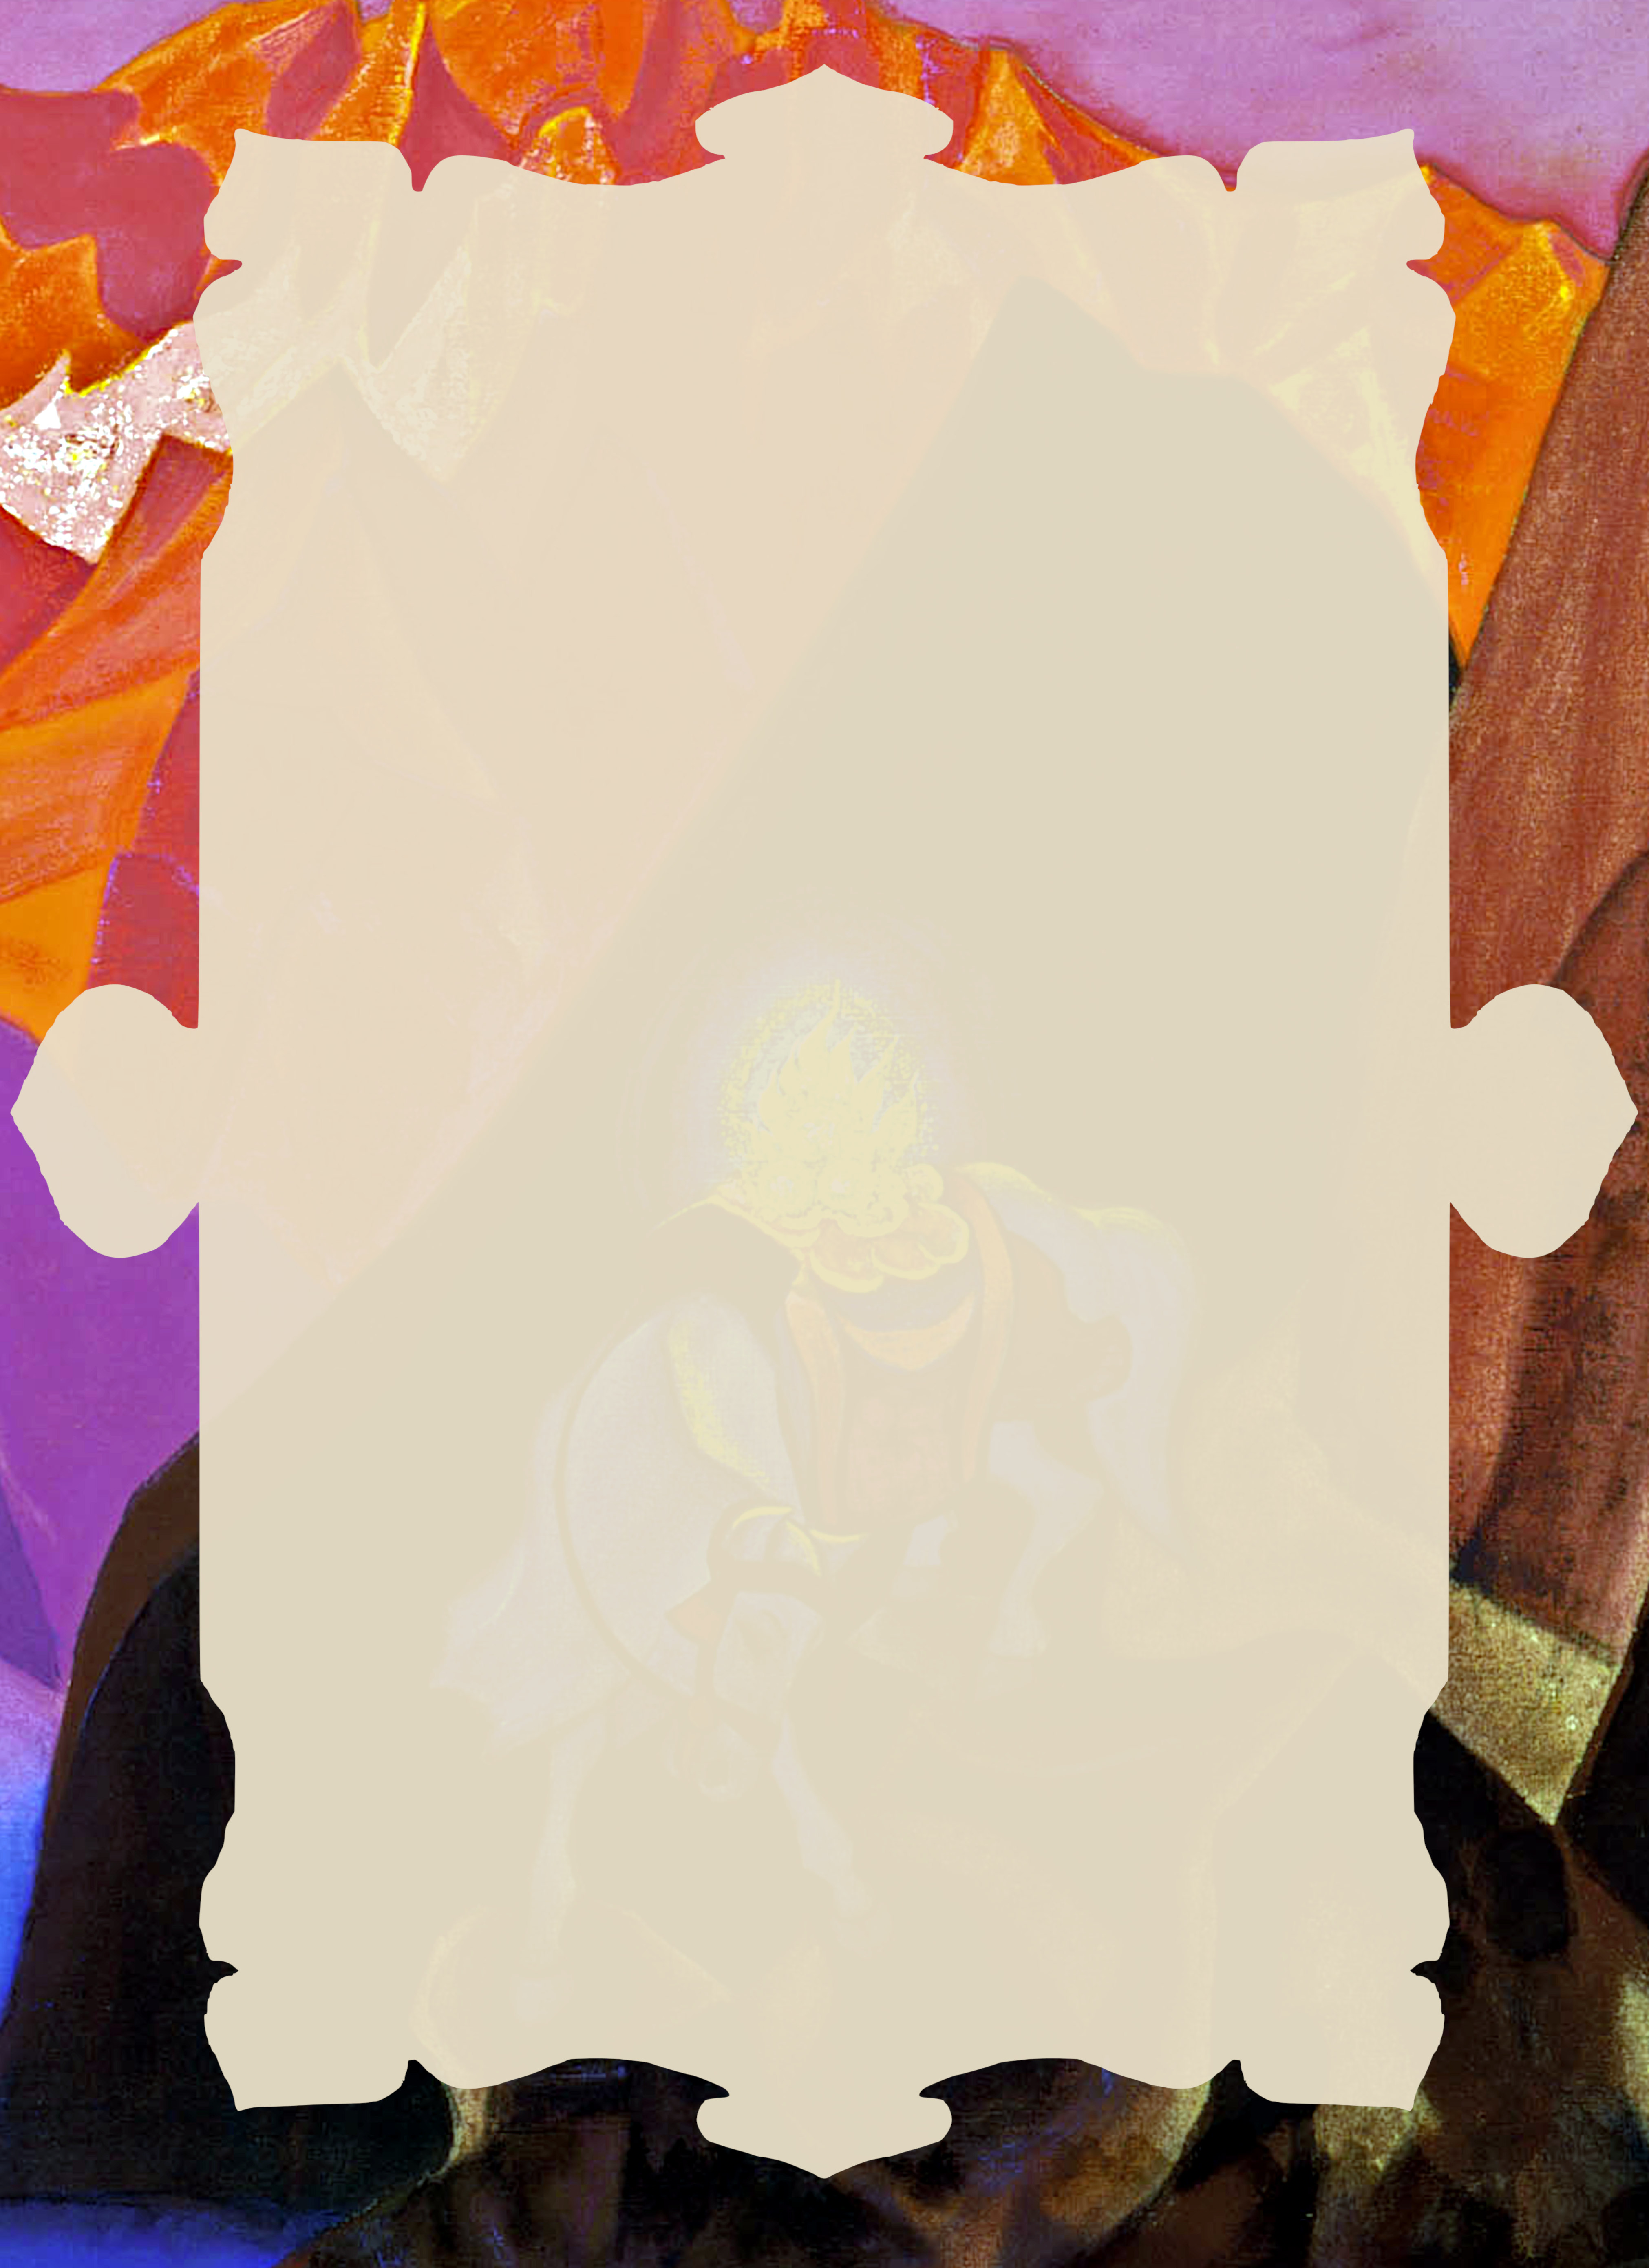
\includegraphics[width=\paperwidth,height=\paperheight]{mountainpearl.jpeg}}
\begin{titlepage} % Suppresses headers and footers on the title page
	\centering % Centre everything on the title page
	\scshape % Use small caps for all text on the title page

	%------------------------------------------------
	%	Title
	%------------------------------------------------
	
	\rule{\textwidth}{1.6pt}\vspace*{-\baselineskip}\vspace*{2pt} % Thick horizontal rule
	\rule{\textwidth}{0.4pt} % Thin horizontal rule
	
	\vspace{0.75\baselineskip} % Whitespace above the title

        {\Huge De Berg van Licht \\} % Title
	
	\vspace{0.75\baselineskip} % Whitespace below the title
	
	\rule{\textwidth}{0.4pt}\vspace*{-\baselineskip}\vspace{3.2pt} % Thin horizontal rule
	\rule{\textwidth}{1.6pt} % Thick horizontal rule
	
	\vspace{1\baselineskip} % Whitespace after the title block
	
	%------------------------------------------------
	%	Subtitle
	%------------------------------------------------
	
	{Door \scshape\Large Louis Couperus \\} % Subtitle or further description
	
	\vspace*{1\baselineskip} % Whitespace under the subtitle
	
	%------------------------------------------------
	%	Editor(s)
	%------------------------------------------------

 	% Subtitle or further description

	\vspace{1\baselineskip} % Whitespace before the editors

    %------------------------------------------------
	%	Cover photo
	%------------------------------------------------
	
	%\includegraphics[scale=1]{cover}
	
	%------------------------------------------------
	%	Publisher
	%------------------------------------------------
		
	\vspace*{\fill}% Whitespace under the publisher logo
	
	Amsterdam 1906 % Publication year
	
	{\small L. J. Veen } % Publisher

	\vspace{1\baselineskip} % Whitespace under the publisher logo

        Internet Archive Online Edition  % Publication year
	
	{\small Attribution NonCommercial ShareAlike 4.0 International } % Publisher
\end{titlepage}
\pagestyle{fancy}
\fancyhf{}
\cfoot{\bfseries\large\Fontauri{\thepage}}
\Large
\setlength{\parskip}{1mm plus1mm minus1mm}
\tableofcontents
\clearpage
\section{Eerste Deel}
\subsection{}
\paragraph{}
In den zoelen nacht van nazomer triltintelden over Emessa aan wijd effen hemel van wolkenlooze nachtkleur de duizende en duizende kristallen sterren, en tusschen de schitterendste vulde de hemelafgrond zich met fijner gepoeier van licht, terwijl daar omheen weêr kleinere dan die zongroote, maar grootere dan zoó poeierfijne geprikt waren in onbenaderbaren overdaad, als waren van starrenweelde de goden dronken geweest, als hadden zij allen, de goden, alle de starren uitgezaaid in zwijmelende lichtdronkenschap. En dwars over dien hemel van weelde blankte de breede en uitvloeiende Melkweg, nauwlijks als een sluier en meer als een glorie, en een pad van triomf voor den oppergod, gepoeierd met lichtstof, gestapeld met sterren, zoo vele, dat de voeten der goden, welke er over heen zouden gaan, daar zeker in verzinken zouden als in een gouden zand, diep.

Onder zoo overdadige nazomernacht lijnden de tempelgebouwen breed, ver, en hoog op, met glans aangegeven kroonlijsten, en met afzonderlijken terrasvormigen toren, wiens top versmalde en vervaagde in het lichtelijke niets. In een dicht bladergeheim van tuinen, stille van wind, lagen in het wijde park de tempel-gebouwen verspreid, blankten nu aangelicht marmer of grauwden dof van graniet, streepten zuilen zich rank, en verloor zich het al in geboomte-schaduwen, waartegen, lichtovergoten van rijzende maan, reusachtige agaven opstaken hare zwaarden òf wit òf zwart, naar mate het maanlicht zijn glans veegde aan de lemmers dier bladeren, of dat zijzelve zich spietsten in schaduw en wègpriemden in nacht. Een oranjegeur zweefde als een wierook, zwaar en bijna onadembaar, en daartusschen hielden de Syrische rozen hare gillende kreten van lustverlangen làng aan... Maar behalve dien geurwalm van bloemen en, twee-, driemaal de snerp van een pauw, heel ver, was geen geluid in de tempelparken en de onduidelijke gebouwenmassa's droomden op in licht, en doomden, en verdwenen verder in aller vormen verzwijmeling tusschen de schaduwopstapelingen van sycomorengeboomte en wierookend citroenheesterbosch.

Af van den lichtterrasgelijnden toren vierkantte donker de Zontempel zelve en somberde weg, en sliep. Nauwlijks verzichtbaarden zich de gedraaide zuilen der zijgalerij, met heel slank getorsadeerde schachten op voetstuk van Perziesch bladornament, telkens herhaald, vaag aangeduid in het nachtlicht, en achter elkander verschoten en verscholen de tallooze zuilen, liepen weg, torsadeerden naar achteren in een lichtschuwe vlucht... Maar heél hoóg slankten zij op, en daar, plots onverwacht, verbreedde heur gebaar van ranke bevalligheid naar links en naar rechts, en kapiteelden zij uit met bijna te stoere kracht, in twee halve stierentorsen, voorpooten geknield in het ijle, de gedeelde achterlijven in elkander versteend, en alle de stierenkoppen met spierbuigenden nek gekromd, zonder zichtbaar de architraaf aan te raken, zoo dat in het nachtlicht de breede fries wel te zweven scheen... Maar de kornis kroonlijstte --- eén zware schaduwstreep --- dwars tegen den startriltintelenden hemel aan, en stille tusschen de zuilen spookten èn schaduw èn licht, terwijl roerloos maar levend reeëel néêr de tallooze stierkoppen staarden.

Breed om het heiligdom trokken zich zoowel zij-peristylia als voorportiek, en zij poortten open van doorgang, duisterende naar de dichtere schaduw der in diepste nacht weggedonkerde apadaña, middenhof van zuilengeschachtte, onafzienbaar en ondoordringbaar, omdat het maanlicht zich veegde aan de uiterste zuilen alleen, de nabij-zijnde dàn even nog aangaf, maar alle de middenzuilen veronzichtbaard hield in het binnengeheim. Toch, telkens duidelijker weêr, verbreedden de zuilen, die zichtbaar bleven, na haar rank-op gebaar, in de hoóge hoogte tot immens kapiteel van dubbelstiertors, en telkens duidelijker kromden de gedrongen stiernekken en staarden met den zelfden starren, maar zoo reeëel levenden blik de tallooze steenoogen naar beneden. Nauwlijks aan die bazalten dierwereld, daar hoog veronbewegelijkt, glimp-te het goud, te fijn voor den nacht aangeteekend in gestylizeerd ijl Perziesch motief. Slechts even leefde het goudgevonk op, beefde een oogenblik en doofde daarna, om elders weêr op te leven. Zoo was het of in het onafzienbare en vooral ondoorzienbare heiligdom het goud wisselend leefde en weêr stierf, langzaam, naar mate heller de maan scheen en rees.

Weêr had --- verweg --- de pauw gesnerpt, toen achter in de diepte der nachtverschaduwde apadaña, meer dan het goud hier en daar, een hellere vonk opleefde, niet zoo stil en metaalzuiver, en meer als een korte vlam, ros, en door een hand overhuifd. De vlam bewoog door de donkerte en telkens smeerde haar rossige glans een geleren striem tegen een zuil...; dan doofde die striem en herhaalde zich, naderend, tegen een andere zuil, terwijl boven de stierkapiteelen òp-halskromden en weêr verdonkerden. Twee gestalten verzichtbaarden aan naar de linker-zijgalerij, en om maanhelte en toortsevlam werden zij duidelijker: twee jeugdjonge knapegestalten, moorzwart naakt de een, die de toorts vasthield, en den vlamglans ervan temperde met zwarte hand, en de ander, --- roze de vlak van zijn overrossigd gelaat, en oproodend in de rossige toortsvlam de hyacinthen mantel, die geheel hem omhulde.

Zacht slopen zij op bloote zool en krakelooze sandaal, toen diè in den mantel opkeek, schuw en verschrikt, en plots zijn witte hand greep den arm van den zwarte, die, gitter dan schaduw, al naderde in den buitennacht. Want van waar zij gekomen waren, uit de diepte der apadaña, ter zijde van immense gordijnen, die afsloten het Allerheiligste, bleekelde op --- hoe ver ook nog van hen verwijderd --- eéne, die hen gevolgd scheen, en wier vaag schemerend driftige plooien wit aan het einde-diep opspookten met de ster van een dofkleine lamp. Tot nauwlijks, na eéne seconde van verkenning in schaduw, een stem schel van bejaarde vrouw riep door de stilte, en de mystieke atmosfeer schril doorsneed:

--- Bassianus!!!

De knaap in den hyacinthen mantel stampte met zijn sandaalvoet, van drift, omdat hij gevolgd werd. Hij greep vaster den arm van den zwarte, en dwong dien met hem te schuilen achter een zuil en in voorzichtige palm weg te houden den gloed van zijn toorts. Maar verscholen, verging dadelijk zijn drift, in giechelende vroolijkheid, en zijn mantel trilde, van zijn kinderlijken lach rillende, terwijl hij fluisterde aan het oor van zijn slaaf:

--- Hoû je stil! Daar is waarachtig weêr het Oude Wijf!

Maar weêr riep die met het sterrelampje --- en de echo's weêrklonken hier, daar, en terug door de apadaña:

--- Bassianus! Bassianus!! Ik ziè je wel!

De knaap had een beweging van ongeduld: hij verschool zich niet meer; hij riep:

--- Wàt is er nu toch weêr, Grootmoeder?

--- Waar ga je heen, Bassianus?

--- Wat deert het u, waarheen ik ga? riep geërgerd de knaap Bassianus. Ga slapen! Ben ik uw slaaf of uw vrijling?

--- Neen, maar wèl ben je mijn kleinzoon, en als ik niet paste op jou, dan zoû niemand op je passen, want je moeder laat je maar doen, wat je wilt! Waar moet dat heen, in den nacht, en den nacht nog wel voór de Offerande? Naar de priesters? Naar de slaven? Naar de danseressen, naar de tempeldeernen, waar vooral dezen nacht iedereen je tegen kan komen, omdat de stad is vol soldaten van het Kamp en vòl vreemdelingen, die bij honderden naar het deernengebouw komen? Of misschien wel de parkpoorten uit en de Oude Stad in, om morgen als de heilige zon hoog staat, bleek terug te keeren, met oogen blauw omkringd? Acht je dan nooit je goddelijkheid, en zelfs niet den vooravond van den Dans? Heb ik je niet hooren slùipen je kamer uit, en heb ik je niet Narr hooren wekken? En wat moet dat: te gaan door het heiligdom; dat je zoo vreemden weg kiest, is wel, Bassianus, omdat je weèt, dat je niet doet als je mag! Gauw, terug naar je bed! Wil je wel gauw naar je bed terug? Wat zegje? Moet ik je halen? Moèt ik je krijgen? Moet ik je om de ooren geven met mijn sandaal?

In zijn hyacinthen mantel stond Bassianus te ledeschudden van lachen, zonder toch uit te barsten, om niet Grootmoeder àl te oneerbiedig te ergeren, maar hij klampte, omdat hij zoo lachte, zich aan zwarten Narr, die wel altijd zijn toorts omhuifde met gitten hand, maar toch ook wròng van pleizier, zich verbijtende, --- hij een slaaf --- opdat de oude Julia Mœza hem niet zoû hooren en hem niet zoû laten kruisigen of voor de beesten gooien. Tot Bassianus uitriep met zijn hooghelle stem, die in gemaakt zangerige buigingen op en neêr weêrechode, spottende jong door geheel de apadaña:

--- Neen Moeder, ik ben vlugger dan u; haàl me dus niet, want u zal me nooit krijgen... En voor de sandaal, hoor, word ik eenmaal te oud! Ik ben vijftien jaren, en ik wil niet meer met de sandaal! Ik wil er niet meer meê! Ik ben niet meer een kind, en ik ben Hoogepriester van de Zon, en ik doe als ik wil, hoor, voortaan! Begrijpt u? Zoó versta ik mijn goddelijkheid! Dat ik gegaan ben door het heiligdom, is eenvoudig omdat die weg korter is naar den Toren, want ik ga dezen nacht nièt naar de slaven of tempeldeernen en niet naar de Oude Stad, maar niet anders dan naar Hydaspes, die mij op het Zesde Terras wacht. Hij heeft me mijn horoscoop beloofd... en ik wil met hem in de sterren lezen en luisteren naar de Geheime Dingen...

Spottende eerst, was zijn gemaakt zangerige stem heel beslist geworden, en de oude Mœza, die nu was genaderd, zag hem hoog en slank voor zich staan, het gelaat achterover in trotschheid en haar metend met zijn lacherigen blik. Maar zijzelve, berouwend haar opwelling van drift, tegen haar lieveling Bassianus, toonde zich niet beleedigd, en kalmer zeide zij slechts, vergoêlijkend haar eerste woede:

--- O, schat van mijn ziel... ga je naar den Toren! Hadt mij dat dan van avond gezegd! Dan hadt je mij niet uit mijn slaap geschrikt, en doen denken aan misdaad en moord en doen vreezen voor jou, o mijn lieveling... Zoo, kind, ga je naar den Magiër... Ga, ga, Bassianus... Ja, het is goed, dat zoo mìn mogelijk weten wanneèr je in de starren leest, opdat geen onbescheidenen pogen te dringen achter het geheim van je Toekomst! O Bassianus, mijn lieve kind, wie meer dan Grootmoeder wenscht die heerlijk en vol glorie, vol stràlende glorie! O, dat ik je nog heerlijk en glorievol zie over geheel de Romeinsche wereld! Dàn kan ik eerst rustig sterven! Zoo, mijn schat, ga je naar den Toren... Ga, ga Bassianus, en ikzelve zal blijven waken tot je terug komt om je den voorhang van je kamer zacht open te houden, opdat nièmand iets merkt, je moeder niet, en Mammea niet, en ook niet de kleine Alexianus... Vertrouw maar op Grootmoeder, kind... Vermijd de tempel-gebouwen en ga liever dwars door de citroenenboschjes, dan kan niemand je zien, mijn jongen... Ga, ga, Bassianus...

De stem van de oude vrouw, van schelle drift en uitbarstende woede, was tot smedige meêgaandheid omgebogen en gaf toe en was het wel eens, nu Mœza meende zeker te kunnen zijn, dat Bassianus naar den Toren en den Magiër ging. Uit de palla, die zij haastig had omgeslagen, stak zij haar hand en aaide hem onder de wangen, waar hij nog trotsch en metende voor haar stond. Hij glimlachte en liet zich, half verzoend wel, streelen, maar toch zeide hij, spottende nog:

--- Kom Moeder, wàt zal u misschien wel den heelen nacht om mij wakker blijven... Ga slapen, ga slapen, Moeder! Ik zal omzichtig terugkomen, voor het nog daagt, en ik beloof u: NIEMAND zal weten, dat ik naar den Toren gegaan ben... Kom, ga slapen, Grootmoeder...

--- Kind, kom toch niet te laat terug. Breng geen slapeloozen nacht door. Maak ons allen niet radeloos. De kleedsters hebben morgen lang werk... Van den dag van morgen hangt veél af... misschien, mijn heerlijke Bassianus... àlles.

Haar stem beloofde geheime dingen en hij zag haar diep aan in de oogen.

--- Weèt u de Toekomst? vroeg hij, met plots ontzag voor haar sibyllischen ouderdom.

--- Neen! verdedigde zij zich.

--- Zeg mij, Eerwaarde, weèt u de Toekomst?

--- Neen, kind, wat zoû IK weten: een oude vrouw, die veel verdriet heeft gehad...

--- Grootmoederlijkheid, ik bid u: zèg mij, zoo ge iets weet?

Hij vleide het, de handen gevouwen, in een gebaar van lief en eerbiedig zijn, en zijn meisjesmooi blank gezicht smeekglimlachte tot haar op, met de dubbelzinnige smachting zijner heel groote violette oogen.

--- Neen, neen Bassianus: IK weet niets... maar àls je mij lief hebt, kind... zèg mij dan morgen, voór de Offerande nog, wàt je met den Magiër hebt gelezen in de heilige starren... Ben ik niet de Moeder, die niet anders dan je glorie wenscht? Maar ga nu, ga nu, kind, en leés de glorie... voor de starren wentelen...

Zij reikte de handen op en streelde hem om de wangen, herhaaldelijk. Zij streelde in hem heel hare eerzucht, en hare zwakheid was, dat zij hem oneindig meer liefhad en groóter wenschte dan haar jongeren kleinzoon Alexianus, den zoon van hare dochter Mammea, hoewel zij niet blind was, en dikwijls zag, dat Alexianus veel eerder de zoon van Antoninus Bassianus Caracalla kon zijn dan haar lieveling, haar ge-incarneerde zonnegod en haar zonnepriester, zoon van haar dochter Semiamira.

--- Ga nu, mijn goddelijke jongen, en leès... voor de starren wentelen! herhaalde zij.

Zij aanbad hem in hare omhelzing. En omziende of niemand gespied had, sloop zij terug, gebogen en dribbelend, eene al bejaarde, maar bewegelijke, levendige vrouw, verdroogd en verdord, behalve in haar eerzucht en in de aanbidding haars kleinzoons: de twee hartstochten van hare ziel... Als van een schim verijlde hare witte palla in de donkerte tusschen de zuilen, en de ster van haar lampje doofde weg, na een allerlaatste opkromming, in de hoogte, van twee-nekkig stierkapiteel.

--- En nu vlug, vooruit Narr! haastte Bassianus den zwarte: hij sprak hem toe met kluchtig volksaccent.

Hooger droeg Narr zijn toorts, terwijl Bassianus zich nauwer in zijn mantel plooide en een punt sloeg over zijn schouder. Zij lieten ter zijde de ris der onder de poeierlichtnacht slapende tempelgebouwen, gingen door de zwaar wierookende citroenheesterbosschen, in bloei... Luchtig en snel achter den toortsslaaf liep op veerende, lichte sandaal de kindjonge Hoogepriester der Zon, slank en heupewiegelend een vrouw gelijk. Speelsch duwde hij den slaaf tot vluggeren gang, en toen Narr, om dit gebaar van zijn meester, schudde de schouders, trok Bassianus' wijsvinger over de gleuf van zijn al spierigen zwarten rug.

--- Wil je wel eens maken, dat je voort komt, Narr! vloekte zijn meester, met straatjongenstermen.

De jonge Moor haastte zich, voortgekieteld. Plots, omdat Bassianus struikelde, greep hij Narr om den hals en leunde aan hem, opzettelijk zwaar, drukte hem nijdig tegen zich aan, en liet hem weêr los, met een sandaalschop, opdat hij voort zoû maken... Maar als Narr zich dan repte, riep Bassianus hem toe, niet zoó te ijlen, en vloekte, dat hij niets zag, en struikelde, en vallen zoû... Veinzende, dat hij viel, klampte Bassianus den toortsdrager dan in beide zijn armen, en voelde in begeerige palmen de spierzwelling van diens al krachtige armen, had een kreet als van een kat in den nacht, en liet hem weêr los en dreigde hem, als hij zich niet repte. Zoo haastte zich Narr, telkens geplaagd, tegengehouden, gestreeld, gepakt en vooruit weêr geschopt, zonder eén woord, alleen met een lachje om zijn dikke zwellippen en een zijlingschen glim in het wit van zijn oog.

De toren terrasde ten hemel; gestapeld als met zes, zeven telkens kleinere dobbelsteenen, bleef zij rank: een trap naar de lucht toe. Zij rees uit sycomoren en een hoogen warrel van Syrische rozen, die stortten haar geur uit wijde roze bekers, en dwars door den geur, bezwijmelend, liepen de beide knapen toe op de poort. Zij was open, als Bassianus verwachtte, en door Narr voorgelicht, ging hij de trap op, die voerde tot het eerste terras. Hoog waren de treden, en om zijne beweging viel ruimer de hyacinthen mantel en sleepte achter hem aan. Onderwijl duwde hij Narr, streek met zijn vinger in diens ruggegleuf, pakte hem, schudde hem in scherts en schopte hem dan, hem zeggende voort te maken. Tot Narr, eindelijk, zijlingsche glim in zijn oogenwit en dikker zwellend de lippen, op de trede zijn toorts wierp, die branden bleef, en met een beweging van drift en een knars in zijn keel zich omdraaide, voor zijn meester dreigend stond, en hèm pakte in zijn vuisten van git, en hem schudde, en hèm schudde. Zoo dat Bassianus Narr een slag gaf met vlakke hand, pats! in zijn donkeren kop. De jonge Moor wilde verder worstelen, en, een jonge hond gelijk, beet hij met zijn zwellende lippen Bassianus in zijn schouder, maar zette de tanden niet en zoende hem op zijn blanke vleesch. Als een kat in den nacht krijschte de knaap Bassianus, sloeg in den kroeskop, die aan zijn schouder zich vastzoog, alle zijn vingers en tròk hem, maar drukte hem tegelijkertijd. De Moor liet niet los en zij worstelden, en toen Bassianus viel, scheurde zijn mantel.

--- Genoeg, Narr! krijschte hij, ontzenuwd. Genoeg! Maak voòrt! Maak voòrt!

Opstaande schopte hij hem. Narr grinnikte blij, raapte de toorts op, en steeg; Bassianus volgde, zich nauwer wikkelend in het soupele hyacinth. Hij hitste Narr niet meer op. Voor een bronzen deur bleven zij staan; Bassianus klopte drie malen.

--- Blijf nu maar hier wachten, Narr...

Ga slapen! zeide hij, gemaakt zangerig en gebiedend zijn stem. Terwijl hij wachtte, hurkte de slaaf al neêr, legde zijn toorts, die branden bleef, en Bassianus leunde de hand op zijn kroeskop; Narr dook in een onder die liefkoozing en bewoog niet meer. De deur opende.

--- Bassianus... wat ben je laat...

--- Ben ik te laat? riep de knaap haastig en zag naar de starren.

--- Neen, niet te laat... Kom in...

Hij greep de hand, die werd toegestoken en volgde. De Magiër leidde hem een binnentrap op, trad toen buiten op het hoogste terras. Daar keerde hij zich om, en zag den knaap diep in de oogen.

--- Mijn lieveling! zeide hij. Wie weet: misschien is deze de laátste maal...

--- Waarom de laatste? vroeg Bassianus. Zoù morgen inderdaad...

Hij voltooide niet: de Magiër omhelsde den jongen. Hij was Hydaspes, de Oppermagiër, een groote gestalte, in sarapis wit; heel donker zijn haren, lang, gekruld om zijn matbleek gezicht, en groot verklaard zijn oogen stralend in transe onder den dubbelen boog der brauwen.

--- Zoû morgen inderdaad...? aarzelde de knaap, herhalend en vragend: hij sprak met gemaakte stem zijn Syriesch zangerig en zuiver uit. Ik weet niet of ik het wensch... Ik geloof bijna, dat ik het niet verlang... Ik ben tevreden met de glorie, die de mijne al is... Ik ben Hoogepriester van Helegabalus, en het volk stroomt toe om mij dansen te zien, en aanbidt mij... Hydaspes, ik verlang niets meer... Het is Grootmoeder, diè verlangt... Zeg mij, làs je het in de starren?

Maar de Magiër ontweek en zeide:

--- Kom hier zitten...

En hij trok op steenen bank den knaap tot zich, den arm om zijn schouder heen.

--- Zie! zei de Magiër. Waren ooit de starren deze maand glanzender! Zie, Bassianus, je eigen star! Daár!! Zij straalt als een zon.

--- Zij is de aarde genaderd...?

--- Neen, zij heft de aarde tot zich toe...

--- Heft zij de aarde...?

--- Tot zich toe...

--- Wat beduidt dat?

--- Misschien het hoogste...

--- Het was wèl Grootmoeders wensch...

--- Misschien...

--- Zeg mij, zeg mij, Hydaspes...

--- Zie... zie dan, Bassianus...

--- Ik zie...

--- Let goed op... Om je gloriezon staan de starren, die haar volgen, dat is: die zijn geweest... Die je voorgaan, zullen komen... Zie, als je lànger ziet, wentelen zij, wentelen zij in eéne beweging, heelalwijd, rondom... Wij, op deze aarde, kind, wentelen meê, vast gesnoerd in hare beweging als aan onstoffelijke koorden... Wij, wij wentelen meê... en als een star zelve, maar getaand tot een tuin, en niet meer als een star stralende, is onze aarde, die bol is, zoo als alle starren zijn bol. Geen vlakke schijf is deze aarde, omspoeld door een hemelzee en ether van oneindigheid, maar een bol is zij, die vurig was ---: eérst droppel van licht uit het Eeuwige, toen òplaaiend tot globe van vuur, toèn doovend, en bloeiend tot bosch... tot wie geest op haar waarden, vermenschelijkten in een immer diepere en diepere vernedering en verbanning van sfeer naar lagere sfeer... Zoo diep vernederd, Bassianus, zijn wij nu... Maar in énkelen van ons licht uit die vermenschelijking onzer ziel de Geest op, en wil terug naar zijn moederstar, en er is werking tusschen dien Geest en de Star. Tusschen beiden weven draden van het heiligste Licht, en verbinden aan zijn star voor eeuwig den Geest, en nauwer en nauwer steeds... als de draden niet breken, en doelloos zweven in het heelal, en dan verijlen als dauw in het niets...

--- Hydaspes... blijven WIJ NIET onbewegelijk...?

--- Kind... zie... zie: zoo als, zoo je heél lange tuurt, je de sterren ziet bewegen en gaan om ons rond, zoo gaan wij om de starren rond, en, bol, gaan wij om onszelve, maar dit, mijn kind, wat ik je zeg, is ons het geheim, het geheim van ons Magiërs, want onze wetenschap is heilig en wij geven ze niet aan het volk. Laat de menigte gelooven, dat Hipparchos te Rhodes en na hem Ptolomaeus in de Thebaïs de waarheid wisten, wanneer zij verzekerden, dat onbewegelijk onze aarde bleef en geheel dit firmament in eéne eerebetuiging neeg rondom ons heen, wij, mijn kind, weten ànders...

--- O Hydaspes... ik huiver soms van al wat je mij vertelt...! Weet dan niemand in Emessa dan jij, onze Magiërs en IK, dat de aarde een bol is, als alle sterren, die meêwentelt met de sterren...

--- Mijn trotsche jongen... neen, denkelijk niet. Wat ik je meêdeel, zijn heilige geheimen, en ik deel je ze meê, omdat ik weet, dat je goddelijk bent.

--- En je weet er zoo veel, Hydaspes...

--- Wij doorgrondden er ènkele maar, Bassianus, om nader tot de godheid te reiken. Onze wetenschap is heél oud. Mondeling wordt zij overgeleverd van ingewijde op ingewijde, en dikwijls, omdat zij de eerste geheimen wisten, vonden de nakomelingen de volgende.

--- Zoo als dat geheim, Hydaspes, dat heel heilige geheim van de Godheid, den Steen, de Monolieth, die stràlen gaat, zoo jij het wilt... Hydaspes, verklaar mij dàt geheim?

--- En vergeten wij je eigen ster... Zie toe...

--- Ja, zij is verschoven, Hydaspes...

--- Zij verschuift steeds, zij verschuift steeds. Maar zoo innig als zij op dit oogenblik zich langs hare onstoffelijke koorden viert aan de aarde en je eigen ziel, o mijn kind, zoo innig vierde zij nooit... En toch!

--- En toch?

--- Verheug ik mij... en vrees ik te gelijker tijd...

--- Wàt zie je?

--- Zoo veèl!

--- Kan je mij niet laten zien?

--- In jaren, jà; niet op eén nacht van lichtgepoeier aan nazomerhemel. Gedurende eén nacht, Bassianus, kan ik je alleen vertellen... wat ik zie...

--- Vertel dan, vertel dan, Hydaspes...

--- Ik zie... de starren, die je volgen, die zijn geweest... Ik staar... En ik ziè ze als de weêrschijningen van vervlogen zielen, en als hàre lichtfantomen gebaren zij daar in den ether... los hare onstoffelijke koorden, die zweven door het heelal, en heel lucht maar doelloos fladderen, als dunne draden op den wereldadem. Verstoord is hun weefsel, en zij fladderen... en, zie!... zij drijven, zij drijven op een zee van bloed!!

--- Op een zee van bloed! O, Hydaspes!!

--- Op een zee van bloed, van bloed! O, zoo veel bloed, zoo veel bloed altijd! Nu ik staar, nu ik staar zonder meer mijn blik af te wenden, nu ziè ik de zee van bloed, Bassianus... Ik zie, ik zie... Het zijn strepen van purper, die golven... Het is een zee, een oceaan van bloed... Bloed van menschen, van dieren, duizende menschen, duizende dieren... Zie, daar... Marcus Aurelius is dood... en het bloed vloeit, dat Commodus, de Gladiator, vergiet: het bloed van àlle zijn slachtoffers, dieren, menschen: gladiatoren en wilde beesten... ze wentelen daar in de lucht àlle rond, stervend in den bloedoceaan... Bloed van een millioen wilde beesten, uit Indische wildernissen naar Rome's arena voorgevoerd aan den Gladiator, zeker van werpspies en pijl... Bloed van honderduizend, wie aanklageren, lasteraars of 's keizers gril dolk of zwaard toedrijven... O, Bassianus, ziè het bloed!! In de bloedzee tuimelen honderd leeuwen van Numidië, stuiptrekken olifanten, snuivebrieschen hippopotamen; in vaart en vlucht ijlen, àl halsdoorsneden, struisvogelen van Mauretanië, die Herakles-Commodus éen voor een den kop afhakt, nog met opene wieken voort!! De Imperator-Gladiator doodt tienduizend gladiatoren... Hun rijke bloed vloeit, en golft! O, de hemel, kind, is eén rood vizioen! Tot zijn eigene bloed vloeit, tot nà hem vloeit het bloed van den Grijsaard, waardigen Pertinax... O, doór het bloed heen, zie ik, kind, Bassianus! de schande van het opbod eens keizerrijks: Rome te koop aangeboden door haar eigene troepen, en zie ik een Consul Rome koopen, het Imperialaat koopen, het purper koopen, omdat hij de rijkste is: Julianus! Hij bloedt: de koopman-keizer; Niger bloedt, Albinus bloedt: zij dompelen allen in bloed, in bloed, omdat Severus opdaagt... de krijgsman... de groote... Septimius Severus...

--- Septimius Severus... o Hydaspes! die Mœza zegt, dat mijn grootvader was...

--- Zie Bassianus, heel de starrehemel drijft in het bloed... Antoninus, Caracalla genaamd...

--- Mijn vader!

--- Ik zie hem: daar! Antoninus doorpriemt in de armen van Julia Domna haar zoon en zijn halfbroêr: Geta...

--- Mijn oom... Geta!

--- Maar hijzelve tuimelt onder in een plas van bloed!! Macrinus, na hem...

--- Bloedt??

--- Nog niet... nog nièt: er purpert nog geen bloed om Macrinus' star! Bassianus, om je eigen star...

--- Purpert bloedt??!

--- Nog niet...

--- O Hydaspes, ik word zoo bang!!!

--- O mijn kind, ik zie niet meer... Rood zwemt het voor mijn blikken... en in dat rood wringelen, klompelen de lijken van menigtes, in een door-elkander-flitsen van zwaarden...!

Als van een kat in den nacht, lang-uit en ontzenuwd, slaakte de knaap Bassianus een kreet en hij klampte zich in hysterischen angst tegen den Magiër en verborg in diens witten mantel zijn hoofd, en wilde niet meer zien, want reeds had hij, in suggestie, den zilveren hemel golven van bloed gezien, en zijn eigen bloed medepurperen: fontein van éen oogenblik, maar dadelijk verzwolgen in de bloedzee, die plengden Heerschzucht en Bloeddorst en Wellust...

Zoo bleef hij, tot de Magiër hem bij de kin oprichtte...

En hij rond keek en zocht naar de zee van bloed...

Hij zag ze niet...

De maan stond heel hoog, en ontsluierde geheel de lichtende goddelijkheid van Astarte-Urania: zij dreef alom en almachtig in dit uur, dat het hare was...

Niet in bloedzee, maar in zee van louter zilveren glans, baadde zij alle de sterren: de groote kristallen, de tot stof gepoeierde en daartusschen alle de andere, kleinere en grootere, doffere en hellere, en zelfs den Melkweg, pad van triomf voor den oppergod, Helegabalus, Hij, die troont op den Berg van Licht, baadde zij verliefd in hare bovenmatige schijnselen. De hemel was eéne sereene straling. In de verte vluchtte de Libanon tegen dien glans langruggig ver weg en tusschen die gebergte-vlucht en stilleren Anti-Libanon dreef Fœnicië in zilveren waas lang uit en wijd heen, terwijl vlak onder den toren zwaar vierkant de tempel droomde en om de in geur slapende parken, de stad, Emessa, wit en verspreid uitgeplekt lag als met groote vierkante en ronde steenen, die in nachtzwijging blankten en meer en meer blankten... Aan de andere zijde van den Libanon dreef de Groote Zee met eén stralende lijn, en de mist van al die klaarte scheen geheel het landschap op te heffen en te verluchtigen, als trok waarlijk de geheele aarde zich hoog aan het onstoffelijke stralenweefsel van Bassianus' ster... De zee dreef, het gebergte dreef, de stad dreef en de toren dreef, alles in lichtwaas en manemist hooger en hooger gebeurd als door een nog grootere dan Magische toovermacht. Een zilveren duizeling draaide om... Neen, Bassianus zag geen rood van bloed: hij zag niets dan glans, van Astarte. Hij ademde den glans, goddelijk element. En een glimlach werd om zijn lippen geboren, terwijl zijne oogen, dubbelzinnig, staarden, staarden in de zilveren vlakte, in de zilveren hoogte, en op nieuw, kalmer, zochten zijn star...

Daár straalde zij en hij glimlachte... Een eerzucht in zijn kinderziel ontwaakte, maar meer om vrome extaze in zilveren nacht dan om wèlke andere reden... Even, voor zijne jongensgedachte, zag hij Rome, waar hij geboren was, op het Palatium van den Palatinus... Onbezorgdheid en kinderspel, met slaven, slavinnen en vrijlingen, tusschen de geuren, gebrand en gesprenkeld, in de kameren zijner moeder Semiamira, de Syrische, zij, de gemalin van senator Avitus, maar wonende met zuster Mammea en diens kleinen Alexianus, op het Palatium, allen samen met de Moeder, Mœza, zuster van Julia Domna, Keizerin; gemalin zij, de tweede, van Septimius Severus, en moeder van diens tweeden zoon Geta. Maar niet Avitus: Antoninus Bassianus, 's keizers oudste zoon, was vader, hèm, den knaap Bassianus geweest, en Semiamira, in trots, had haar zoon naar dien vader genoemd. Antoninus Bassianus, dat was de wreede, de kort breede stoere, de ruwe soldaat, wiens tronie het kind zich herinnerde, wulpsch zinnelijk, met laag kort voorhoofd onder dik kroeshaar, neus en mond gedrongen, de oogen van wellust om bloèd vooral toegeknepen, en breed zijn kaken als van een beest. Caracalla, zoo noemden --- omdat hij den Gallischen mantel, caracalla, droeg en deed dragen --- de soldaten hem, die hem aanbaden; hij, eenvoudig soldaat als zij, slapende als zij allen in legertent, verorberende als zij allen de smakelooze soep, sterk als niet een, en zijn wapens dragende, en zelfs de zware adelaren vaak torsende. Caracalla... nièt Avitus, was zijn vader geweest; ten minste zoo verhoovaardigde zich Semiamira, zoo verzekerde het grootmoeder Mœza wie het maar hooren wilde, in fluisterend geheim, met vrouweverzoek nièt over te klappen, maar trotsch hopende op algemeene openbaarheid na dit in geheim geschonken vertrouwen... Toen was keizer Caracalla vermoord, en Macrinus, zijn moordenaar en opvolger, had niet geduld, dat de oude Mœza met dochters en kleinzonen twee, te Rome op het Palatium blijven zoû en, Syrische zij, was zij met haar gezin verbannen naar haar geboorteland, uit de grootheid van Rome terug naar Emessa, de stad van den Zonnetempel, waar het Hoogepriesterschap erfelijk was in haar geslacht. En had Mœza in Rome niet schatten verzameld, zoo vele, dat niemand wist, waar zij ze borg, en hoe vele milliarden sestertiën ze telde, en had Mœza met zoo veel goud niet de Magiërs geheel op haar hand gehad, zoo dat zij in den Zonnetempel almachtig was geworden in heel korten tijd, en hijzelve met zijn jongeren neef Alexianus tot den Heiligen Dienst werd gewijd, waarin Bassianus --- lenig, slank en androgyniesch van leden mooi --- al spoedig uitmuntte onder àllen in den Dans, rondom den Zwarten Steen...?

En dadelijk, te Emessa, had Bassianus gevoeld, dat hij geen Romein was in bloed, maar Syriër, Aziaat en Oosterling. Nauwlijks ontwassen der prilheid van kinderjeugd, had hem dadelijk in Emessa verrast een lucht, atmosfeer, vreemd bekend, die hij glimlachend inademde; het bloed zijner grootmoeder, Mœza, DE Moeder, het bloed zijner eigene moeder jubelde dadelijk in hem met eene blijdschap, en hoe onbezorgd zijne kinderjaren ook waren heengebloeid in de kameren dier twee vrouwen op het Palatium, te midden van de geuren en soupele stoffen, gemmen en gepolijste spiegels van dat gyneceum --- te midden van àl de slavinnen, die hèm baadden en balsemden, als zij zijn moeder baadden en balsemden, en hem krulden de haren, en het blond ervan met goudstuifsel poeierden, en hem de schoenlinten omstrengelden, tot onder de knie, waar zij ze vastklampten met groote camee --- tòch was het hem in Emessa, of hij in Rome altijd iets gemist had: een zoele glimlach, die in de lucht om hem aandreef, glimlach van sympathie en begroeting; warme kus van bekende wellusten; omhelzing, mysterieus en mystiek, of hij, onbewust, kind, iets gemist had, dat hem nu zoo overdadig overstelpte... Die stad, die tempel, die eeredienst om den Zwarten Steen, fallus-symbool van Helegabalus, die geuren, die dansen, die kleeding --- het was hem alles, zoo vreemd, bekend, ook al zwolgen zijne verraste zinnen het in voor de allereerste maal --- als een vergeten droom, die zich plots verwerkelijkte: werkelijkheid, waarin zijne ziel dadelijk inheemsch en sympathiesch samensmolt. Die starrewichelaarstoren, de apadaña met de stierkapiteel-zuilerijen; de priestergebouwen links, waar hij nu huisde in het Hoogepriesterlijke Hof, met grootmoeder, moeder, tante Mammea, en den kleinen Alexianus, te midden van meer dan honderd Zonnepriesters, duizend slavinnen, die zich vermengden met nog eens duizend tempeldeernen en -dienaren en -slaven: die stad-op-zichzelve, in het hart van Emessa, mystiek en wellustig; geheimzinnig vol occult geheim van door de Magiërs verborgen Kabbalisme en tegelijk religieus ontuchtig in ceremonie en tempeldienst --- het deernengebouw rechts, aaneenschakeling kleiner vertrekken onder hooge zuilenportiek, niet anders zijnde dan een bordeel ---: die stad kènde de jonge knaap Bassianus; die mystiek en die wellust wìst hij, had hij reeds vele malen geweten, en er verbaasde hem niets, en het glimlachte en liefkoosde hem alles toe met stroomingen, geuren, weêrschijnen, klank van fluiten en slag van cymbels, licht en schaduw, zonschijn en starregepoeier --- of hij de prins was van dat zwoele rijk, die weêr terugkwam tusschen al wat hem behoorde en bloed-eigen was. Niet meer dan een glimlach in de lucht en een liefkoozing van effluve was dit den knaap, die zeker nooit vermoedde, dat hij zoó zeer het eigen, bloed-eigen kleinkind was van de oude Julia Mœza, die hem bromde en vleide en knorde en streelde en aanbad, maar om de ooren gaf met de sandaal, als hij te lang zoek was geweest in de zijgebouwen en er gevonden werd met een slaaf, in donker geheim. De prins van die zwoele wereld; neen, het verbaasde hem niets, dat hem, knaap van veertien jaren, door het priester-college, bewerkt door Mœza, die vele duizenden sestertiën strooide, het Hoogepriesterschap van de Zon werd opgedragen, opdat hij zijne slanke knapenaaktheid in ritueele dansen wringen zoû voor den Steen. Hij was er de prins, hij werd hoogepriester: het gebeurde alles zoo als het gebeuren moest en er was niets verwonderlijks of vreemds in: hij was de prins en de priester van die tempelstad geweest van heél klein kind af...

Eén oogenblik, voor zijne jongensgedachte, flitste dit alles heen, niet als duidelijke overdenking, maar als een effluve en een geur, terwijl de Magiër bij de kin den knaap had gericht, die in den wijden hemel geen bloed zag, maar glorie... Zijn eerzucht droomde het hoogste, maar droomde het alleen om de seksueel-mystieke bezwijmeling van dat hoogste, dat hij zich voorstelde als eene vergoddelijking op de aarde van zijn Hoogepriesterschap: een dichter naderen tot den god Helegabalus... Die eerzucht was gevoed door de grootmoeder, die in Bassianus àl hare hoop stelde om terug in Rome te komen, terug op het Palatium en terug tot de hoogste trede der oppermacht, maar de knaap zelve zag die oppermacht vooral als zijn Zonnehoogepriesterschap over geheel de wereld...

--- Hydaspes, zei Bassianus kalmer. Er is geen bloed... in den hemel meer...

De Magiër glimlachte, geheimzinnig en weemoedig.

--- Neen, mijn kind...

--- Het was een vizioen...?

--- Van de waarheid...

--- Die voorbij is...

--- ...En misschien nog komen zal...

--- Hydaspes... Zag je mijn bloed...

--- Neen... neen...!

--- Waarom zoû je het mijne niet hebben gezien... als je het zag van zoo velen, zoo velen, die...

Hij aarzelde.

--- Die wat, mijn kind...

--- ...Geraakten tot de Oppermacht?? Hydaspes, zeg mij: zàg je in de sterren rondom mijn star niet, dat IK geraakte tot de Oppermacht...?

--- Ja... Ik zag... Ik zag...

--- MIJ keizer, zoo als Mœza het wil?

--- Ja, kind. Ik zag je keizer...

--- Je zag mij keizer?!

--- Ja.

--- Waarom aarzelde je het mij te zeggen?

--- Is mijn wetenschap volkomen zuiver? Zoo ik verkeerd zag...

--- Neen, je zag niet verkeerd, zei de knaap Bassianus bijna weemoedig. Ik voél, dat je goed zag... Ik word keizer. O, ik word zeker keizer... Al is het niet voor van daag of morgen, dan word ik het toch over drie maanden, zes maanden, een jaar... Je zàg het bloed van Macrinus... Wie hem treffen, roepen mij uit... Ik weet niet of ik het wensch... Emessa is mij liever dan Rome... Mijn Hoogepriesterschap is mij zoo dierbaar als mij het Imperialaat nooit zijn kan... Maar ik zoû Hoogepriester der Zon worden over gehéel de wereld! Daàrom alleen zoû ik de Oppermacht wenschen... Toch, ik weet niet... Hydaspes, zeg mij: lees de sterren verder voor zij zich heelemaal wentelen... Zie, de mijne nijgt al over den Libanon heen... Lees mijn toekomst: o vlug, Hydaspes...

--- Kind, ik zie de toekomst niet meer... Zoo veel bloed als ik zag, heeft mij verblind en ik zie niet meer wat zijn zal... Maar wèl...

--- Maar wèl...?

--- Wel weet ik, hoe ik wilde, dat je was, als je keizer werd.

--- Hoe, Hydaspes, zoû je dan willen, dat ik was? Zèg het mij! Ben ik niet de vriend van je hart, van je lijf, van je ziel? Heb je mij niet altijd gezegd, dat je nooit, vrouw noch man, hebt liefgehad als je mij lief hebt gekregen, sedert den nacht, dat ik voor het eerst de zes terrassen beklom om met je in de starren te leeren lezen... Ik was een slechte leerling... Ik heb niet veel geleerd... Maar onze avonden samen... zijn ze mij niet het lieflijkste en het geheimzinnigste en het waarachtigste van mijne heilige Initiatie, Hydaspes? Ik ben sòms niet meer dan een stoute jongen, ik ben sòms Hoogepriester van Helegabalus... maar HIER, in deze zee van extaze, ben ik niet anders dan je gehoorzame, vertrouwende vriend, die je aanhangt met heel zijn hart, met heel zijn ziel... Zeg mij: hoe wil je, dat ik zijn zal, als ik oòit keizer word...? Ik wil, dat je het mij zegt! Je woorden zullen mijn wet zijn! Ik ben een kind, en weet niet voor mijzelven... Word ik keizer, dan zal het Mœza zijn, de Moeder, die voor mij zal heerschen... Maar word ik keizer, dan wil ik heerschen niet volgens haar wil, maar volgens de heilige Magische wet, volgens je eigenste wensch, o mijn Hydaspes... Zeg mij, HOE wensch je mij, mocht ik oòit reiken tot de Oppermacht??

De knaap Bassianus vleide: zijn hoog helle zangerige stem streelde en drong als om een gunst, met al de weeke buigingen van de stem eener behaagzieke vrouw: hij had de kleine handen gelegd tegen de schouders des Magiërs; hij zag met zijn dubbelzinnige oogen, die als donkere violen waren --- vreemd, vol smachting en lonkende spot, vol verlangenden ernst en dartele dwaasheid: de blik van een sfinx en een meid te zamen --- diep in Hydaspes' hèl zwarte transe-oogen, die bijna uitdrukkingloos glinsterden als starre diamanten, en liefkoozende legde hij zijn hoofd tegen den baard van den Magiër, zoo dat deze rook den geur van de gemuskeerde myrrhe zijner licht goud overpoeierde krullen.

--- Kind, hoe ik je wensch...? Zeg het mij zelf...

--- "`Doende het groote Goede?"'

--- Ja.

--- "`Strevende naar het Allichte?"'

--- Ja.

--- "`De heilige Zon aanbiddende?"'

--- Maar vooral het heilige Licht...

--- "`Waar de Zon het heilig symbool van is..."'

--- Ja, maar waarom wij niet het heilige Licht vergeten...

--- "`Onzen Lichtdienst met mij meêdragende, door heel het Rijk, tot Rome toe?"'

--- Zeker.

--- "`Alle keizerlijken invloed aanwendende... om den Dienst van het Licht te verbreiden... onder alle volkeren, die aan Rome zijn?"'

--- Ja... ja...

--- Hydaspes, zoó wensch je me dus... mòcht ik geraken tot de Oppermacht...

--- Zoo, Bassianus, in de openbaringen van je leven, maar meer nog en anders in de heilige stilte van je ziel.

--- Hoe daar in...?

--- Hoor mijn kind... Wij streven terug naar het Licht, waaruit onze ziel, een vonk, weggetikt werd in de ruimte der eeuwigheid, tot zij viel in steeds dieper vernedering, en rossigde tot onreine vlam, en verstoffelijkte tot een ziel van goud, want goud is het verstoffelijkte licht en in het Goud schuilt de ziel, vernederd, des Lichts: daarom is het Goud wereldsch symbool van het hoogste, en het rijkste, en het machtigste, en het lichtste...

--- Ja. Dat heb je mij al verklaard, Hydaspes.

--- Onze ziel streeft tot haar oorsprong terug; de ziel van goud, die hier op aarde, zoo zij niet geheel vervièl, leeft om het goud en er henen streeft, die ziel streeft tot haar Oorsprong terug; die ziel wil terug tot het Licht... Onbewust, bij hen, die niet weten: bewùst, en meer en meer, bij hen, mijn kind, die ingewijd werden en weten. Bij òns streeft zij bewust...

--- Hydaspes, streeft mijn ziel bewust...

--- Nog niet! glimlachte de Magiër. Maar je bent nog een kind, Bassianus.

--- Moet ik ouder worden naar mijn bewustheid toe...

--- Zeker...

--- Leer mij...

--- Trek alle je gedachte te samen, af van de wereld, en vestig ze als een bundel van lichtende stralen...

--- Op de Zon?

--- Op het Licht...

--- De Zon is het Licht.

--- Het symbool alleen van die Heiligheid.

--- Ik begrijp...

--- Poog de ziel van het symbóol te doordringen.

--- Ik zal pogen: àlle gedachte, af van de wereld, terug te trekken om ze te vestigen, als een bundel van stralen... op...

--- Het Licht zèlve.

--- Ja, ik begrijp...

De knaap sloot de oogen, als poogde hij.

--- Ik begrijp, herhaalde hij.

--- Maar niet alleen van de wereld, ook van jezelven, Bassianus, moet je terug trekken alle gedachte...

--- Van mijzelven?

--- Van jezelven... Vergeten, wie je bent...

--- Zelfs al ben ik keizer.

--- Zelfs dan... Juist dàn... Vergeten, dat je keizer bent, vergeten wie je bent, wat je bent, en terug streven tot den Oorsprong...

--- Tot den Oorsprong...

--- Van Licht, die God zelve was.

--- Het Onuitsprekelijke...

--- Ja.

--- De Onuitsprekelijke God.

--- Ja. DIÉ.

--- Ik begrijp, ik begrijp.

--- Vergeten, dat je keizer bent.

--- Wie ik ben...

--- Wàt je bent, en terugstreven, in metamorfoze na metamorfoze, tot een Oorsprong, die inheilig, was sekseloos...

--- De Oorsprong, die sekseloos was...

--- Voór HET, in geheim ondoorgrondelijk, de Geboorte dacht en de Schepping, en beide seksen in zich borg.

--- De Oorsprong...?

--- Die, inheilig, oorspronkelijk sekseloos, dàcht Schepping, Geboorte en zich vermannelijkte en zich vervrouwelijkte tegelijkertijd tot het Man-Maagdelijke Licht.

--- Ik begrijp.

--- Het Licht bevruchtte zichzelve: zijn eigen godmannelijkheid omhelsde in al-eerste Liefde zijn eigen godin-maagdelijkheid.

--- Ik begrijp.,..

--- Goden werden geboren.

--- Ja.

--- In een regen van zonnen en starren.

--- Ja.

--- De Harmonie was dadelijk.

--- Ja.

--- En is in de hoogste sferen altijd gebleven.

--- In de sferen der goden.

--- Zij verbrak in de menschelijke sferen... De menschen zijn de kinderen der goden, vernederd om geheimzinnige boete: niemand weet waarom en om welke Zonde...

--- De Zonde is het Geheim.

--- Ja.

--- Wàt Zònde is weet niemand.

--- Juist, mijn kind.

--- Maar Zonde is...

--- Zoo leerde ik je.

--- Ik heb dàt niet vergeten... O, ik had zoo gaarne, dat je mij zei het geheim, dàt jij weet: hoè de Steen gaat stralen op het heiligste moment van den Dienst!

--- Laàt dat, kind, zei de Magiër ongeduldig. Dat is bijna een geheim van geen waarde.

--- Zèg het mij.

--- Ik zeg je waardvoller geheimen... Dwaal niet af.

--- Neen...

--- Je wil weten, hoè ik je wensch, in het stille geheim van je ziel, mòcht je keizer worden.

--- Ja...

--- Ik zoù je wenschen strevende terug tot den Oorsprong, die sekseloos was.

--- Voor HET...

--- Schepping en Geboorte dacht, en beide seksen in zich borg...

--- Maar om te bereiken den zielstoestand van het sekselooze Licht...?

--- Moet de Uitverkoren Ziel eerst terug streven tot dien menschelijker vorm: de vorm der Tweeslachtigheid...

--- Ik begrijp.

--- Moet de Uitverkoren Ziel terug streven tot de androgynische ziel van de Man-Maagd.

--- Ik begrijp...

--- Zoó was onze eerste Vader...

--- Adam...

--- Adam-Heva...

--- Ja, zoo was hij... toen hij woonde in het Paradijs aan den Eufraat.

--- Adam-Heva was hij, onze Vader; Man-Maagd was hij, tweeslachtig en enkel-dubbel... Maar zoo als het Licht, sekseloos, zich splitste in zich tot Man en tot Maagd, zoo splitste --- o ondoorgrondelijk geheim des waaroms! --- Adam-Heva, na een hevige smart over zijn wezen, zich tot twee: tot Adam, tot Heva...

--- Tot Man en tot Maagd...

--- Tot Man en tot Maagd... Voór hij zich splitste, in zijn droom van smart en onvruchtbaar verlangen --- want het was hem niet gegeven zich te bevruchten, zoo als het Licht zichzelve bevrucht had --- spilde hij iederen nacht de essens van zijn wezen, en op die verspilling stortten zich de demonische larven, die, demoniesch, ons altijd omringen, ons, nageslacht van den Man en de Maagd...

--- Ik begrijp, ik begrijp, Hydaspes...

--- Dus de Uitverkoren Ziel streeft terug tot den vorm der Tweeslachtigheid.

--- Ik begrijp...

--- Tot den vorm van de Man-Maagd...

--- Het Enkel-Dubbele...

--- Het Enkel-Dubbele... O Bassianus, zoû je de Uitverkoren Ziel zijn... Zoo velen zag ik, maar niemand, die mij zoo zeker deed denken, en bijna weten: hij is de Ziel Uitverkoren... Want zij moet zijn ernstig en levensblij, de Ziel; een ziel van vroomheid en een ziel van liefde, een ziel van extaze en van wellust beide, een ziel van geinitieerde wijsheid en een ziel van kinderlijke dartelheid: zoo is de Uitverkoren voorspeld, in een lichaam, als een kostbare vaas vol schoonheid; rank de efebe-leden, maar rond de schouders en borsten, de leest dun en de heupen breed, de beenen krachtig, maar luchtig de voeten van zweving, het gelaat zuiver gesneden en vlekkeloos, de mond smachtend en de oogen àl stralend van het gewenschte Licht... Bassianus o mijn Bassianus, ben je zoo niet? Niet te vrouwelijk, niet te mannelijk, de beide seksen in evenwicht versmolten tot een harmonie...

--- Ja, ja, zoo ben ik, o Hydaspes... Ik ben zeker de Uitverkoren Ziel! Ik zal zijn Man en Maagd, beiden... En ik zal... ik zal... Maar, o Hydaspes, zèg mij nu ook het geheim van den Steen, die strálen gaat...

--- Kind, het is een natuurmacht, die wij weten aan te brengen: meer niet, om het fallus-symbool, den Steen, van het groote Symbool, de Zon --- het symbool zijner mannelijkheid --- indrukwekkender voor het volk te maken. Kind, wat doet het er toe... Het is geen geheim van waarde... Het brengt ons niet tot het Lìcht dichter... Bassianus, ben je de Uitverkoren Ziel...

--- O, ja, ja, Hydaspes!

--- Streef dan, mijn kind, tot het Licht...

--- Door den vorm heen van het Enkel-Dubbele, de Man-Maagd...

--- Streef zoó, streef zoó!

--- O, Hydaspes, ik zal zoo streven, en ik zal bereiken, ik wìl bereiken... In de extaze van dezen nacht voel ik, weèt ik, DAT IK BEREIKEN ZAL... Ik zal Man-Maagd zijn! Ik zal Adam-Heva zijn! Ik straal terug tot het Licht, tot het Licht...

Het was of de hemel zich opende en den Berg van Licht, waarop Helegabalus troont, reveleerde... Maar achter den Libanon daagde het roze...

En de starren, eéne voor eene, verwelkten...

De maan verbleekte en verschimde weg; de Groote Zee zilver-rozigde, haar einderstreep getrokken tegen de nog even nacht-kleurige westerkim...

Buiten aan de poort sliep Narr, toen Bassianus hem met een schop wakker schrikte.

De jonge Moor, zwijmelsluimerend nog, greep zijn uitgebrande toorts...

--- Voort Narr, maak voort! riep Bassianus; eng trok hij de punt van zijn hyacinthen mantel over den schouder.

De toortsdrager ging hem voor, door de in morgen opklarende citroen-heesterbosschen, toen, plots onverwacht, Bassianus hem sprong op den rug.

--- Voort Narr, voort en draàg me!

De slaaf greep zijn meester bij de enkels voorzichtig, en Bassianus hing Narr over den rug, beide zijn armen gesnoerd met den klamp van zijn handen rondom Narrs hals, die bijna stikte in die steeds nauwere worging. Het was nog even een laatste spel; zij bereikten den tempel, in de apadaña sprong Bassianus af, wierp zijn mantel Narr over den kop, strikte er vlug twee slippen van vast...

De Moor rukte en rukte: hij bevrijdde zich als uit een strik, en zag zijn meestertje gierende door den grijzen morgenschemer der zuilen verdwijnen achter een voorhang. Tempelslaven, al bezig, kwamen verbaasd te voorschijn... Maar Narr gaf geene verklaring, vouwde den mantel over zijn arm, en haastte zich zijn heer achterna, naar het Hoogepriesterlijke Hof. Er dreef nog de rust van den laatsten slaap... Toch hoorde Narr Mœza's stem, en, bang, verschool hij zich:

--- Foei Bassianus, is dàt laat terugkomen... Grootmoeder heeft niet geslapen... op je gewacht... En wàt heeft Hydaspes gelezen...

Narr hoorde Bassianus geeuwen, heel luid, en zeggen, dat hij nog slapen wilde... De oude vrouw sloop spoedig terug naar haar eigene kameren...

Voor het peristylium was een waterwerk, waar drie krokodillen, onbewegelijk, lethargiesch, geketend lagen, terwijl eentonig klaterend de drie stralen der kruik-uitgietende Danaïden nooit vulden het ronde, groenmossige vasculum... Duidelijker, in den eersten morgen, zuilden de gebouwen op, verschoten de nog wazige diepten der parken en de pauwen trippelden nader... Zoodra Mœza verdwenen was, sloop de Moor te voorschijn, lichtte den voorhang van het slaapvertrek op, en trad in... Bassianus, dadelijk, was in slaap gevallen...

Hij lag op zijn lage leger van zijde geel, het hoofd op een geel zijden kussen, achter, aan ringen, een geel zijden voorhang, door Mœza zorgzaam toegeschoven. In de allereerste opalen morgenklaarte, die in de geheel vergulde binnenkamer dommelde te samen met bruingouden schaduw, lag de knaap Bassianus bloot en blank op den buik over de geelzijden matras, in de houding van Hermafroditos, het hoofd op de gebogen armen. En hij sliep, na ernst en dartelheid, vast en sereen. Over de dubbelzinnige oogen waren ovaal de scheelen, azuur omcirkelde schelpen, gesloten. Zijn adem ging reeds, als een ruischen, de diepste diepte van den slaap te-gemoet. Een lichtende watering, een vloeiende lijn liep in het gedommelde licht over zijn rug, over zijn welvenden onderrug, zijn beide gestrengelde beenen, slank. Aan zijn voeten glansden de gepolijste nagels en, hoewel naakt, had hij vergeten de camee-ring van zijn tweede teen af te schuiven. Bij het bed slingerden zijne losgestrikte sandalen; in het midden der kamer stond bij een groote vergulde waterkan een groote kom van geel amber... Over een drievoet-schabel slingerde uit een schipvormigen bak van email, door tritonen getorst, een snoer van gouden plakkaten, gegraveerd geheimzinnig, aan iederen plakkaat een karbonkelen fallus... Langs een onyxen tafel glansden metalen spiegels op, en schitterden kruikjes te voorschijn, en overal, aan het verguld en het geel, aan de zijde, het amber, het onyx, aan de karbonkelen van het halssnoer begonnen, heller en heller, vonken te leven met de glimpen van het beginnen des dags. Blank en bloot lag, in diepsten slaap, als Hermafroditos, Bassianus.

Narr zette zich op den grond tegen het leger te leunen, en toen hij in slaap viel, zonk zijn zwarte kroezehoofd tegen den voet van zijn meestertje aan. In slaap bijna, kuste de Moor dien voet en hij glom gitter, in het goudener daglicht, tegen de geelzijden matras...

Buiten, in de deernegebouwen, begon het leven te ontwaken...

Uit een lage deur, tusschen eene opklimming van blauwe convolvulus, verscheen eene tempeldeerne, loom; onder hare borsten had zij opgeknoopt een azuren lap, die viel voor haar neêr met druiping als van zwaar water...

Zij rekte de armen hoog op, en wijd uit, moê van den nacht...

Een pauw, vlak voor haar voet, sleepte zijn staart vol oogen, en, toen zij geeuwde, snerpte de vogel zijn korten en schellen kreet.

\subsection{}
\paragraph{}
Het leven ontwaakte; uit de lage deuren van het deernengebouw, eene voor eene, traden de vrouwen, begroetten elkaâr, verhaalden elkander haar nacht. Door de opene tralie-ramen waren sommigen binnen zichtbaar, zich gereed makend voor den Dienst, de Offerande, en den Dans. Zij blanketten elkander, terwijl slavinnen haar schoeisel om de kuiten vaststrengelden met de kruislingsche linten, die reikten tot onder de knie. Een geur van gebrande nardos dreef, op de zwaardere zwoelte van rozenolie. Buiten, in het peristylium, bereidden slavinnen blanketsel en kosmetieken: zij doopten papavers in water, voor het rood van de lippen; gerst en eieren vermengden zij met hertehoorn, die in het voorjaar was afgevallen; zij stampten narcissebolletjes samen met honig en gom; zij wreven iris van Illyrië met loodwit en nitrium rood; zij zeefden de slijm, waarmede de ijsvogel haar nest bereidt, en die, licht opgelegd, een schitterende blankheid geeft. Uit de open gelaten kruikjes walmden de vette parfums, waarover de vliegen al zwermden; de citroenbloesems, enkelsterrige bloemetjes, geurden zwaar; morgenbries woei aan de ziel der Syrische en Perzische rozen. Over het deernengebouw strekten zich lang de portiek-gebouwen der zonnepriesters. Ook zij verschenen, de meesten reeds gereed, in wijdmouwige samaren, die sleepten; de mitra op de gekrulde haren. Zij waren meestal zeer jonge lieden, knapen nog, enkel kinderen van edele afkomst. Zij zagen niet naar het deernengebouw; van haar gescheiden door de bloesemende heestermassa's der parken, maar door het gelooverte heen wezen de deernen naar hen, en noemden hun namen en giechelden, fluisterden, en noemden namen met de hunne samen. Lammeren blaatten; zij kwamen aan, roomkleurige wemel van wollen dierrug-gen, dicht op elkaâr, voortgestuwd door de staven der herders; rammen volgden: de slachtoffers voor de Offerande; zij werden naar kooien geleid achter het daklooze Allerheiligste, waar de Zwarte Steen werd aanbeden. Slavinnen liepen af en aan; zij droegen op de armen gele, hyacinthen stoffen; kleine kofferen tegen de borst; op den schouder langhalzige kruiken. Een ruischen van stemmen steeg hooger, waar tusschen het blèren en blaten van lammeren en rammen, en het snerpen van pauwen, meerdere, meerdere pauwen: rondom de waterwerken sleepten zij de tinkelende oogen hunner staarten en zij dronken tusschen de lotosbloemen, ijdel de gekroonde koppen, nuffig de halzen, langzaam klokkend de kelen. En het bruischen der stemmen lawaaide voller en hooger met het lachen en roepen en schelden en haasten en vloeken der deernen op; de jonge priesters echter wandelden langzaam kwijnend, vol minachting voor alle die vrouwen: de danseressen, fluitspeelsters, cymbelslaagsters, tokkelaarsters der Egyptische sistra; allen weinig geacht, veel gezocht --- niet door hèn --- door de mannen der stad en soldaten der Fœnicische en Syrische legioenen.

Een oude negerin dribbelde aan.

Zij droeg een rood- en geelstrepig hemd, open op de borst en hare borsten bengelden, slappe kalebassen, links en rechts. Zij klapte ongeduldig de palmen; zij riep met Moorsch accent, waarom giechelden de vrouwen:

--- Ho dan, ho dan, Statyra, Livilla, Myrrha, Xylitta...

Zij riep er nog meerdere; zij kwamen, haastig, omdat de negerin Vasthi, de opperste der ornatrices van Zijne Heiligheid zelve, de palmen bleef klappen; zij kwamen: een zwerm van tien vrouwen naakt, danseres-en-ornatrix; alleen waren zij geblanket en gekapt en droegen zij het Syrische schoeisel, met drie cameeën, boven elkaâr, de kruislingsche beenlinten bevestigd. Uitgekozen om schoonheid, monsterde Vasthi ze van het hoofd tot de teenen, zoó, dat zij verlegen giechelden en zich verborgen achter elkaâr.

--- Livilla, ga terug naar je kamer! zei de negerin Vasthi.

--- Waarom?

--- Je haar zit scheef en slecht zijn je brauwen getint, en bleek en blauw zie je van je nachtdienst.

Livilla begon te huilen, pruilende met vuurroode lippen, maar bleef.

--- Xylitta, hooger de gesp onder je rechterknie.

Xylitta boog zich en morrelde aan de camee; het was Statyra, die haar moest helpen.

--- Naar je kamer, Livilla! dreigde de negerin.

--- Ik ben de rechterschoenbindster van Meestertje! wierp Livilla tegen.

--- Maak eerst, dat je er beter uit ziet...

De meid had een beweging met arm en schouder; zij ging naar haar kamer terug.

--- Vooruit! zei de negerin tot de anderen.

En zij volgden haar, op eén gelid, bijna militair, maar wiegelend de heupen, en niet giechelende meer; heel ernstig. Zij gingen het park door; gaande voorbij het priestergebouw, werden zij heel verlegen onder de hooge, laatdunkende blikken der wijd-gesamaarde jongelieden, die vaag de trotsche oogen òver haar richtten en haar niet schenen te zien, zich om hunne man-vrouwelijkheid achtende van hoogere essens. De deernen volgden Vasthi tot in het peristylium van het Hoogepriesterlijke Hof. Daar bleven zij wachten; vooruit ging Vasthi en wenkte Narr, die buiten zat te droomstaren naar de drie krokodillen. De Moor stond op, keek langs den voorhang van Bassianus' kamer: toen trok hij den voorhang weg.

De knaap Bassianus was juist ontwaakt.

Hij had niet bewogen; hij lag in de houding van Hermafroditos.

Het zonlicht, door vergulde tralie's heen, scheen hel op de vergulde wanden der kamer, en de schelle kleuren der fresco's --- dansende callipygen, schoonbillige androgynen, zich achterom in laag gehouden spiegels beziende --- scharlaakten, okerden, vleesch-kleurden heviger op. Vonken schoten de vergulde kan, de amberen kom, het halssnoer, en vlakkeloos blank, met eéne golving van gratie, rekten Bassianus' ranke leden over de geel zijden matras, die goudgloeide.

Vasthi verscheen in de deur; zij boog kluchtig, de handen hoog opgestrekt.

--- Uwe Glorierijkheid... daar zijn de kleedsters!

De knaap Bassianus glimlachte, spot tintelend in de schelmsche hoekjes van zijn dubbelzinnig geknepen oogen: zijn mond trok nòg kleiner, als tot een zoen samen.

--- Goed Vasthi... Waarschuw de Moeders.

De negerin boog ten tweeden male, trad buiten en zij gebood Statyra de genadige Semiamira en de verhevene Mœza te verwittigen. Toen wenkte zij de andere vrouwen. Achter haar, in militair gelid, traden zij binnen, stonden zwijgende op een rij.

--- Is het dan heusch al zoo laat! zei Bassianus.

Hij geeuwde.

--- Eerst het bad; vlug Narr!

De jonge Moor kwam; zeide, dat het bad gereed was.

--- Vasthi, help je me met Narr in het bad...

Het bad, rood marmeren bekken, rond in het midden van aangrenzend vertrek, was een fontein: vier dolfijnen spoten water, ijskoud, koud, lauw en heel heet. Narr opende de kranen en Bassianus, aan Bacchus gelijk, blank en bevallig, rondde zijn rug onder de stralen beurtelings. Het bekken liep vol: hij dompelde aan de hand van de negerin en hij sprong vroolijk, hij lachte, hij wierp haar met water. Zij stroopte de mouwen op, en ving hem geheel in ruige dwalen, waarmeê zij hem wreef. Hij had zich gezet op een schabel en Narr wreef met ronde puimsteenen hem gelijkmatig over de dijen.

--- Deborah! riep Vasthi. Polijst de nagels van Zijne Zongoddelijkheid!

Zij stapelde, in hare adoratie, de meest exotische titels, verzon Bassianus maar altijd mooiere namen. Maar Deborah knielde en nam in den schoot Meestertjes voet, heel hoog gewreefd, hol van zool, zonder éen fout aan den vorm der teenen. Hij kriebelde haar tusschen de knieën; zij deed of zij niets merkte en zorgvuldig polijstte zij de voetnagels glimmend.

In het slaapvertrek woelde een beweging, begon een onrust, omdat de oude Mœza en Semiamira met hare vrouwen waren binnengekomen, nog ongekleed, om tegenwoordig te zijn bij de kleeding van Bassianus. Zenuwachtige stemmen riepen en haastten dwars door elkaâr, omdat het al zoo laat was. Mœza zeide, dat zij verboden had eerder Bassianus te wekken; Semiamira verklaarde, dat hij nooit klaar zoû zijn op het heilige, ritueele uur. De slavinnen gonsden dooreen, al was haar het zwijgen geboden; de zenuwachtigheid steeg, omdat Bassianus maar niet uit het bad kwam. Hij liet zich geheel door Narr met puimsteenen wrijven, Deborah glanzender de teennagels polijsten en Vasthi, met tangetjes klein, trok hem de enkele haartjes uit, onder op zijn rug, op de armen, waarna zij de trilling van de opperhuid dadelijk zalfde met een streeling van hare zwarte vingers, die zich gedoopt hadden in een roze schuim.

--- Bassianus! riep Semiamira.

--- Bassianus! riep Mœza.

--- Ik kom...

Hij kwam, zijn blankheid door het bad rozig vertinteld. Hij duwde de dienvrouwen links en rechts, zoo dat zij struikelden --- eéne viel --- en als een stout kind plofte hij neêr op den stoel voor de tafel der spiegels. Reeds had Statyra de ijzers gewarmd; niemand als zij, die het haar wist te kruiven, luchtig, donzig en zonder te branden. Zij kruifde vier lokken aan iedere slaap; de lokken in den hals kruifde zij voller en ronder; ze vielen over de schouders heen. Het was heel gewichtig, allen zagen toe; toen Statyra daarna met een dons vochtig goudstuifsel gepoeierd had over de lokken, die als werden verguld, zei Semiamira:

--- Nu moet ik mijzelve kleeden...

Zij ging met hare slavinnen; de oude Mœza bleef.

Maar bij de deur van het peristylium was een gegons van twistende stemmen, want Livilla kwam terug en Vasthi, nòg ontevreden, riep heesch en gedempt:

--- Je haar zit nòg scheef: terùg naar je kamer...

--- Ik? riep verontwaardigd Livilla. Ik ben Meestertjes rechterschoenbindster! Ik, terug naar mijn kamer? Hoe kan hij dansen zonder dat ik hem bind en ontbind?

--- Deborah zal den rechterschoen bedienen...

--- Deborah? riep de meid jaloersch. Doet die het beter dan ik? Neen, mij... mij is het toegestaan...

Mœza vroeg wat er was; Vasthi klaagde, dat Livilla schaamteloos was en er uitzag als een meid van de straat; de knaap Bassianus riep:

--- Livilla!

--- Meestertje!

Zij stortte toe, knielde neêr.

--- Livilla, pas op straks de linten van den rechterschoen, die jij bindt en ontbindt, goed over en weêr te strengelen... Als je je vergist, laat ik je villen, zei Bassianus, terwijl hem Statyra nu schilderde onder de oogen, steeds met haar zekeren glimlach, zonder eén beving der vingers, die vasthield de stift antimonium.

Vasthi dorst niets meer zeggen; Livilla triomfeerde, trotsch, voor de negerin. Onderwijl beijverden de vrouwen zich om Bassianus, meerendeel om ter sluik te bespieden hoè Statyra toch handig en zeker, en zonder eén fout, het gelaat van Bassianus schilderde, het geheel belegd had met een ijsvogelslijm-email van wit, voor zij de wangen rozigde. Maar de oude Mœza was niet tevreden.

--- Het is tè veel! riep zij uit. Veel te veel! Statyra, dat is te veel! Vasthi, zie toch, dàt is te veel! Moet een frissche mooie jongen als Bassianus zich laten schilderen als een oude hoer? Neen, Statyra, dat is te veel!

Maar Bassianus had zich over en weêr in alle de spiegels bekeken, die de vrouwen, knielende, met hoog geheven handen reikten.

--- Ach, Grootmoeder, het ìs niet te veel! riep hij ongeduldig en stampte met den voet, die nog maar los slipte in een muil. Het is niet te veel! Bedenk toch: u ziet mij hier, u staat op mij; daarom lijkt het te veel. Maar het is niet te veel. De apadaña is bijna donker en de zon stroomt op het heilige uur fel in het daklooze Allerheiligste, en als ik dans, dans ik geheel in de zon. Ze zien mij dus uit den donker in fel licht en Statyra verstaat haar werk, want als zij mij niet zoó emailleert als ze doet, heb ik geen gezicht, ben ik alleen een vage vlak in de verte! Bedenk toch, hoe reusachtig de afstand is. Wie achter staat ziet mij als een vlak, niets dan een vlak, wanneer Statyra mij niet hèl schildert.

--- Maar je huid, kind, bederft, van zoo dikke laag...

Bassianus haalde de schouders op.

--- Deze zalf, Eerwaarde, zei Vasthi en toonde een kruikje; wascht dadelijk na den Dans geheel de laag af...

En een gegons van de vrouwen om Mœza heen, beduidde haar, hoe eerbiedig ook, dat zij zich moest vergissen, en dulden moest zij, dat Statyra het lichaam van Bassianus, die was opgestaan, geheel bestreek met een liquide zalf wit, die dadelijk zilverig droogde... De vrouwen zagen angstig toe, want eens was een kleedster gegeeseld geworden ten doode toe, omdat zij met striemen de zalf hadden gesmeerd. Maar Statyra, trotsch zeker met dunne lippen, die zelfgenoegzaam glimlachten, ijdel op hare kunst, smeerde de zalf met lange streken van haar borstel, van den hals tot over de voeten, en zoo luchtig was hare hand, dat niet eén streep te ontdekken was. Alleen, toen Bassianus gekieteld, door den borstel tusschen zijn beenen, een plots gebaar maakte, en met een giechel zich schudde, hield zij op, verschrikt, de hand, den borstel in de lucht. Zij werd bleek. Maar er was niets bedorven en zij herhaalde haar streek. De knaap stond parelig wit, onwaarschijnlijk zilverig blank: Afrodite, het schuim ontstegen, kon niet zilveriger zijn geweest, en zelfs Mœza was wel tevreden.

Maar onder de vrouwen begon grootere zenuwachtigheid te trillen, want Bassianus zoû worden geschoeid, en dat was het allergewichtigste van zijne kleeding voor den Dienst en den Dans. Daar tijdens den Dans van den Hoogepriester, rondom den Steen, vóor het allerheiligst moment --- waarop men aannam dat de erbarmende Ziel van de Zon zelve neêrdaalde en zich incarneerde in den Middelaar tot Man-Maagd --- de rite wilde, dat twee vrouwen den Hoogepriester, terwijl hij zich wrong en wendde, de lange linten van het schoeisel ontstrengelden en dit daarna weder op het zelfde rythme aanbonden, en vastklampten de gespen drie, moesten de tempeldeernen, wie deze eer toeviel, zeer zeker zijn van haar taak, moesten zij in de kleedkamer des Hoogepriesters zelve ieder den schoen, die haar aanging, vaststrikken en zich ook maar niet in het minste vergissen in de wijze, waarop de linten zich over en weêr strengelden tot onder de knie. Het was Livilla, die den rechterschoen bediende; Xylitta bediende den linkerschoen. Terwijl Mœza en alle de vrouwen in cirkel toekeken, schoeiden zij Bassianus, terwijl hij even schetste den danspas, en de deernen de hymne murmelden; eene begeleidde met fluit, andere met trom, dat, zeker op maat, de bewegingen harmonieerden der beide ornatrices, die bleek zagen van spanning. Livilla vergiste zich, strengelde eén lint boven, terwijl zij beneden moest omgaan, en Bassianus werd razend, stampte, en stompte haar in de borst met zijn vuist. Maar zij herhaalde en zij verbeterde zich, en nog eens, en nog eens werden de schoenelinten gestrengeld en de cameegespen vastgeklampt: dat moest met eene beweging geschieden en er mocht niets aan ontbreken: anders zoû de Dans zijn ontheiligd.

--- Het zal wel gaan, Uwe Zonheerlijkheid zei Vasthi, wier dikke lippen trilden van zenuwigen angst.

Buiten weêrgalmden slagen van gongs, heel hoog en weêr laag, heel schel en dan dof, en zij dreven de geloovigen ten tempel. De Menigte stroomde aan de zonpoorten al aan, om goede plaatsen, vooraan, te nemen, en tot in de Hoogepriesterlijke gebouwen en het Vrouwehof, die een wacht van Romeinsche veliten omringde en afsloot voor wie wellicht nieuwsgierig tot daar dringen zoû, klonken de gillachen en het blijde gejuich, want groote feestdag was de driemaandelijksche Uitoefening van het Sacerdotium. Het gonggegalm deed in de peristylia de deernen zenuwachtiger zich haasten, zich verzamelen; ook de zonnepriesters kwamen al aan; ook de huiveringwekkende Magiërs, allen wachtende op Bassianus, glurende binnen zijn kamer, hij, de allereenigste, die kalm glimlachend bleef. Trouwens, nu hij geschoeid was, was hij zoo goed als klaar. Het zware goudplakkatensnoer over de borst, en de plakkatengordel hem om de lendenen, aan iedere plakkaat, gegraveerd symboliesch, een helroode karbonkelen fallus, en daar de Hoogepriester, tijdens den Dienst vóor den Dans, het Sekselooze Licht symbolizeerde, daalde de gordel van het midden der leest langs de liezen tot het lid toe, dat een ronde schulp van karbonkelen ving, zoo dat geen sekse bleek. Sekseloos stond Bassianus en naakt, geschoeid, gegordeld, gehalssnoerd. Nu zette hij zichzelven de mitra op en vier vrouwen brachten den mantel, rond sleepend, wijd van mouwen, en sloegen hem voorzichtig dien om de schouders. Hij gaf er een lichten kreet om: de mantel was zoó zwaar, dat hij meende in een te zinken onder het gewicht, maar hij kreunde, gelukzalig:

--- O...! Hoe zwaárder mijn mantel mij drukt, hoe záliger ik me voel!

Het was een wellust zoo buitengewoon, dat bijna angstig de deernen rondom hem staarden, huivermystiesch bedenkende, dat Zijne Heiligheid goddelijken lust ondervond, die haár nooit werd geopenbaard. Nu stond Bassianus in zijn klokkemantel van goud en juweel: stijf stond de geheel overstikte, heel zware Syrische dubbel-zijde, en de rand der gemmen richtte zich recht van den grond op.

Buiten weêrgalmden de gongs.

De immense koperen bekkens, regelmatig en rythmiesch geslagen met zware klepels, weêrechoden schel en gedempt, hoog en laag, over en door de parken, daverden heen en daverden weêr tusschen de gebouwenrijen, wier massa's de klanken opvingen en ze weêr kaatsten terug, zoo dat zij zich versprenkelden tusschen de rozenheesters en citroenenbosschen en de verspreide gouden echo's de al warme zonnelucht deden sidderen. En de vibratie was zoo hevig, dat wel de rozen wuivende trilden, dat wel de vlammen dwarrelden der geuren, die in het peristylium de slaven onder toezicht der thuriferariï ontbrandden in lampen en geurvaten, dat wel eén jubel zweepte de zinnen en zielen van àl wat leefde in dien gloriënden morgen; de gongs jubelden, en jubelend gonsde de Menigte over den stoffigen voorweg áan op den tempel: geheel de atmosfeer weêrdaverde van jubel en trilde in een nevroze van zinnelijke verwachting. Alleen de zonnepriesters, die nu allen verzameld waren in het peristylium rondom de Magiërs, bleven kalm en laatdunkend glimlachend: de meesten niet ouder dan knapeleeftijd, sleepten zij hunne lange samaren over het mozaïek, allen de mitra op, wachtende op Bassianus. Toen Mœza de Hoo-gepriesterlijke vertrekken verliet te midden van haar slavinnen --- zij nog ongekleed in witte palla, zich haastende naar het Vrouwenhof om zich ten spoedigste te dossen in feestkleedij --- weken zij allen ter zijde uit: de Magiërs, de Priesters-der-Zon, schaarden zich, en begroetten haar met kruipkrimpende nederigheid. Zoó gejacht was zij, dat zij niet terug groette. Maar op den drempel van het Vrouwenhof verscheen Semiamira, in gouden chlamys, het haar hoog in den vorm half Romeinsch, half Assyriesch op-gekapt tot een toren, azuuroverpoeierd, en omspannen met spangen saffier. Langs hare dochter haastte oude Mœza zich, zeggende, dat zij heel gauw klaar zoû zijn. Het peristylium bruischte van stemmen en haastiger weêrdavergalmden de gongs, de slagen ranselende in elkaâr en tegen elkaár: het was of al dat geluid stuk sloeg en met atomen in de lucht tusschen den zonneschijn bleef dwarrelen... Boèngh!... Boèngh!... bonsden de slagen der gongs, boèngh! op elkaâr en lieten elkander geen tijd meer: zij rommelden als gouden donderen, heel laag over de parken, en zij spatten uit tegen de zijgebouwen; zij sprongen op tegen den tempel, zij sprenkelden verder over den starretoren omhoog...

Zwerm van fluitspeelsters, tamboerijn- en cymbelslaagsters, sistra-tokkelaarsters drong aan, naakt, maar gekapt, geschoeid en geschilderd: zij werden geleid door eunuchen; andere eunuchen, ceremonie-meesters, verzochten de zonnepriesters zich op te stellen; nomenclatoren riepen namen en nummers; een troep slaven ijlebeende aan, bijna te laat, gedreven door hunne opzieners...

Op den drempel van het Hoogepriesterlijke Hof, verscheen, omringd van zijn dienaressen, Bassianus, ernstig als een god, stijf omstraald in zijn priestermantel, klokke-uitstaand en hem verbergend geheel: alleen zijn gelaat, hèl goud omkruld, onder de heel hooge mitra, was boven dien stralenden klok zichtbaar als een bovenmenschelijk aanschijn, strak, star, en verworden tot godegelaat in het email van zijn wangen, het vermillioen van zijn lippen, den zwarten dubbelboog boven zijn oogen, die bleven als van een sfinx en een meid... Zijn eigen dienpriesters, genoemd door de nomenclatoren, geleid door de eunuchen, haastten zich naar hem toe.

De gongs sloegen boènghende tegen den tempel en over gehéel Emessa sprenkelden zij de millioenen vonken en atoom-uitspattingen van hun onweêrstaanbaren oproep.

\subsection{}
\paragraph{}
Een stuiveling witte stof poeierde van den weg omhoog, om de haastige stappen der aanstroomende, -stroomende menigte. Langs de hooge cactushagen, de tempelparken omstekelbladerend, stroomde de Menigte van links en van rechts toe naar de zonzuilen-ingang, en met het gouden gesidder der gongslagweêrtrillingen vermengde zich, tot hoog in de lucht, het poeierende stof, opgejaagd door de duizende en duizende zich reppende sandalen, en wemelde weêr glinsterstuivelend neêr. Veelvuldige beweging van zwaaiende armen gebaarde daaruit, koortsig en enthouziast; stemmen gonsden en riepen en schreeuwden; getemperd door de stofwemeling spattevlakte de feestkleedij van de Menigte toch nog schel in den gloedgloor der zon, die uit een gouden gat aan den hemel blauw goot alle haar licht zonder voorbehoud: de witte weg scheen met kleurstof, die voortbewoog, oversmeten. Geroep van slaven, stafgebaar van lictoren, geschommel van toegegordijnde draagstoelen, snel spaak-aangewarrel van hooge carpenta, waarin men zat of recht stond, gehinnik van zebra's, gebalk van muilen aan basternae gespannen, veroorzaakte immense beweging en duizend-geluidige ruzie over den weg, tusschen de twee stroomen der altijd en altijd maar voortreppende kleur-gespatvlakte voetgangers, en zoó dicht stuivelde het stof op en poeierde weêr neêr, dat overal was een verblinding van oogen, een geproest en geschraap van kelen, een gefnies van neusgaten, een gespuw uit naar alle zijden --- en dàn een gescheld om die kwalsters, een vuistend gebons op elkaár, een gevloek en getwist, maar dadelijk medegeslierd door de achterop aankomende massa's. Aanrazende met een zee van geluid, goud overdonderrold door de boènghende, boènghende slagen der gongs, stormvloeide met een stroombocht zoo links als rechts de massa door de zonzuilenpoort in de parken.

De breede weg naar den tempel was aldaar afgezet door het Stedelijk Cohort, onder bevel van den Stedelijken Tribuun; langs de voorportiek en den gesloten hoofdingang, straks van den Optocht bewaard, rijde zich de kavallerie der loricati, verguld geschubkurasd en verguld overhelmd, speerlans gesteund in koker op knie, en tegen de slankte der hoog in de hoogte stierkapiteelende zuilen trokken, op hun goudschabrak-overdekte hengsten, zij een breed machtige streep van gelijkmatigen schubbigen glans, fel schitterend tegen het zondoorstoofde bazalt.

Maar de zijpoorten waren alle wijd open, en trots het militair vertoon van het Cohort der Kavallerie en het politie-toezicht van het Stedelijk Cohort, stroomde de Menigte aan weêrszijden de apadaña binnen met haar zwellenden, zwellenden vloed. Als met een snellen rivierbocht door sluizen boog zij van links en van rechts binnen de zonzuilenpoort, maalstroomde over het tempelplein, golfde daar tusschen de aaneengesloten hastati, dragers van lansen, òp tegen de Kavallerie, en dan draaide zij uit naar de zijpoorten, met een ronden kolk van kleuren, koppen en zwaaiende handen.

Zij was gekomen van overal.

Zij kwam van Damascus, van Tyr; van Sidon, van Heliopolis, van Palmyra; zij kwam zelfs van Jeruzalem. Zij had dien nacht in Emessa alle herbergen niet alleen overvuld, maar zij had in den starrennacht van verwachting zich gelegerd waar maar een stoep, een trede, een steen was te vinden, zoo zij niet geslapen had in het maandauwige gras. En toen de eerste gongslagen waren geboènghd en haar op naar den tempel van Helegabalus riepen, was zij beginnen te stroomen, samen te stroomen over den witstoffigen weg, in koortsig voorgenot, opgewondenheid dol, zoo als zij ging, de Menigte, naar ieder spektakel, naar ieder spel, naar iedere vertooning en optocht, maar doller, opgewondener, koortsiger om vrome vereering van den God van de Zon: en om zijn Hoogepriester en Incarnatie, den jongen Bassianus, dànsen te zien, rondom den Zwarten Steen. De roep van zijn goddelijke gratie had zich na iedere driemaandlijksche Offerande verspreid en de Dag van den Grooten Dienst en den Dans was geworden tot een zonnefeest van jubelende opwinding, voor welke zelfs de groote feestdagen in de tempels van Heliopolis verbleekten en veronbelangrijkten. Neen, naar Emessa stroomden Syriërs, Fœniciërs en Joden --- om het heilige kind, den kleinzoon van de fabelschatrijke Mœza, dansen te zien. Wie hem gezien had, ging weêr; wie hem niet had gezien, hoorde zoo veel van dien andere, dat hij ging, dat hij, was hij arm, de laatste dagen niet at, om enkele drachmen over te leggen als reisgeld. Maar gaan naar Emessa den Dag van den Dans ging ieder, die niet lam, blind of ziek was. Aanzienlijken kwamen met kemelen en stoeten van slaven; ouden van dagen kwamen op krukken en moeders sleepten haar kinderen meê; bedelaars drongen bij honderden de menigte door en telkens sloegen gauwdieven hun slag.

De Menigte stroomde binnen de apadaña, en dadelijk suisden stille de bruischende stemmen, of zij met kalmte overgoten werden, maar ook de oogen, verblind door zon, stof en kleur en beweging, baadden dadelijk weldadig in schaduw en over de bezweette leden heen liep zelfs even een rilling van kilte. Veliten, lichtgewapend, zetten een breed pad af dwars door het midden der apadaña, door tusschen de zuilen hun lange speren horizontaal te houden op de hoogte der borst, van den vrij gehouden hoofdingang tot de trappen toe des Allerheiligste. Zware gordijnen, die hingen als met bronzen plooien, sloten dit af voor de oogen der Menigte, en zij had nog niet anders te doen, dan zich zoo spoedig mogelijk, dringende, dringende, te stellen vlàk bij het heiligdom, elkander misgunnende een duim verdere en dichtere en betere plaats. Dringende, dringende in elkanders ruggen, stond zij als opgepakt en kon zich niet meer verroeren, een mozaïek gelijk geworden van star starende koppen vòl geduld om te wachten nog ùren lang, voor de Optocht binnen zoû komen en de bronszware gordijnen zouden openwijken. Uit dat mozaïek geduldige koppen, als uit een hoogeren vloer slankten de schachten omhoog en te vele waren de zuilen, vonden zij, die gedrukt tegen een schacht, gevaar liepen verpletterd te worden, of, èrger, van den Dans niets te zien... Slankten de schachten omhoog en boven, in een door ènkelen zonstraal lichtgoud gepoeierde wemeling, staroogden over de Menigte neêr de dubbelstieren der kapiteelen, de gedeelde lijven in elkander versteend, voorpooten geknield in het ijle en torsende op steenen kussens de cederen balken der zoldering, fijn oversponnen met goudachtig Perziesch blad-ornament, dat voor de gewende, in schemer gebaadde blikken, duidelijker begon te glansen.

Onophoudelijk drong dichter de Menigte. En al viel hier en daar een vrouw flauw, werd, nog meêlijdende, buiten gebracht, of raakte een kind, schreeuwende, onder den voet. Maar een bende van vijf, zes gladiatoren was binnen gedrongen en zij openden zich met de breedte van hunne schouders, opgezette borsten en gespannen spierarmen een brutalen weg, om de zuilen heen, door de mozaïkmassa heen, die schold, van den voet werd gestuwd, op elkaâr werd geduwd, hijgende in elkanders buiken en ruggen en knieën. De gladiatoren stoorden zich niet; torenend en massief, bonsde regelmatig hun bende vooruit en de voorste, een mirmillo en Germaan, riep luid tot zijn makkers:

--- Vooruit maar, vooruit maar, nòg dichter bij!

De anderen volgden den Germaan, brutaal lachende, maar nog meér werd de Menigte gepakt en geprest toen een troep Romeinsche legionariï binnen hoste, en er ontstond een gedrang: vrou-wen schreeuwden en gilden, messen werden getrokken. Een walm van knoflookadem en uitwasemend zweet dwalmde al op, vermengd met de bitterheid van stof van de straten, de sterke kosmetieken der vrouwen, terwijl van achter de bronszware gordijnen al aannevelde een aroom der ginds bereide lampen en geurvaten. Achter de gladiatorenbende hield zich een Indiër strak geparst tegen hen aan; hij was naakt, met een lap om de lendenen; even kopergebruind, zijn hoofd in witten tulband omwonden; mager en slank bevallig hield hij de gladiatoren bij, liet die voor hèm den weg banen en ging met hen meê en stuwde vooruit achter hen aan en won zoo steeds een betere plaats. Nu, glimlachend zacht, had hij zich listiglijk weten te duwen tot midden in hun spiervleezige groep en stond er als in een bescherming en veiligheid: zijn lippen glimlachten, zijn oogen glimlachten, terwijl hij staarde op het bronszware gordijn.

--- Zeg, vriend, wat moet dat? vroeg de Germaan.

--- Jullie zijn sterk, ik niet, zei de Indiër met zachtvleierig vreemden tongval in zijn zangerig Syriesch; de zwakke zoekt steun bij den sterke. Ik ben van uit het park achter je aan gekomen. Hier hebben wij een vrij mooie plaats om den Dans van Zijne Heiligheid aan te zien.

Hij sprak formeel en beleefd, met zachte stem, glimlachte steeds, rustig veilig in de groep der gladiatoren, waarin hij zich dichter nestelde. Hij had den rug van den Germaan tegen zijn borst; links en rechts presten hem twee zware Galliërs, achter hem drongen twee retiariï en een belluarius, maar hij liet zich pressen en dringen, nauw gevangen omprangd door de monsterlichamen, van spiermassa's zwellend tegen hem aan, de ruwe beestachtige koppen kijkende over hem heen, omdat hij kleiner was.

--- Is het de eerste keer, dat je Bassianus zal zien dansen? vroeg de Indiër aan den mirmillo.

--- De eerste keer, antwoordde, kort, de Germaan.

--- Ik heb je gezien, den laatsten keer in de Spelen, glimlachte vleierig de Indiër. Je bent Gualterius; nu, je bent genoeg bekend. Ik heb je bewonderd. Je hebt je retiarius neêrgelegd met een kunst als geen ander bezit. Je bent niet alleen heel sterk, maar je kent ook je vak, als niet éen. Dàt was kunst, hoor, zoo als jij hem legde.

De mirmillo brulde op, breed, van pleizier.

--- Ja, ja, het was goed! blufte hij, welbewust.

--- En zien jullie den goddelijken Bassianus ook voor het eerst? vroeg de Indiër heel beleefd, met een ronden blik tot de anderen.

--- Ja, ja! beaâmden zij.

--- Wij hebben hem wel eens zien offeren...

--- Maar nooit nog zien dansen...

--- Ja, van daag zien wij voor het eerst hem dànsen.

--- Nu, zei de Indiër; dàn zal je wat te kijken hebben!

--- Zag jij hem dan wel eens dansen?

--- Wel vijf maal. Het is iets, dat je noóit hebt aanschouwd en noóit na hem meer aanschouwen zal. Het is een genot voor je oogen en voor je hart. Ik ben Ganadasa, de gymnosofist, ik kom van den Ganges, en ik dacht veél te hebben gezien, maar ik had niets gezien voor ik den heiligen Bassianus zag dansen. Goden, wat is dat mooi! Zie je, ik ben gymnosofist, ik heb gestaard op mijn navel, om mij van de wereld af te trekken en op te gaan in de Onzienlijke Dingen, maar sedert ik Bassianus gezien heb, ben ik niet meer gymnosofist --- trouwens, van staren kan je niet eten --- en sedert ik Bassianus zag dansen, ben ik aanbidder van de Zon en aanbidder van Bassianus! Goden, wat is dát heerlijk, die Dans... Je oogen worden geboeid, maar dàn wordt je ziel gevangen. Je kàn het niet weêrstaan. Het is een betoovering. Het is een wonder.

--- Ja, ja, zei de mirmillo; het is een wonder, dat zeggen allen.

--- Dring nòg verder op, ried zacht vleiend de Indiër, en uit zijn lendedoek gleed hij in den poot van Gualterius een halve aureus.

De gladiatoren bonsden naar voren; zij scheidden de nijdige menigte in twee; nu naderden zij tot vlak bij het heiligdom, aàn tegen de wacht der veliten.

--- Hier zie je àlles!! zei de Indiër Ganadasa. Hier zie je de estrade van den Proconsul, van de Prefekten, van de drie Moeders! Dàt is een goede plaats! Laten we ons hier niet van wegjagen, hoor!

--- Daàr zullen we wel op passen! bralden de gladiatoren.

--- Zeg vriend, zei de eene Galliër, en pakte den Indiër rondom zijn middel, zoekend in den plooi van zijn lendedoek. Heb je voor mij ook niet een aureus?

--- Zeker! glimlachte de Indiër. Kijk maar eens hier...

--- En voor mij? En voor mij? drongen de anderen om Ganadasa, tot hij gekneed was tusschen de massa van dij en van biceps.

--- Zeker! glimlachte hij onveranderlijk. Kijk maar eens hier! En kijk maar eens hier!

En hij drukte hun allen in de zware knuisten goudstukken, die hij listiglijk tooverde, zij wisten niet van waar, want zijn lendedoek was heel los en heel smal.

--- Je bent een rijkaard voor een filozoof van den Ganges! zei de mirmillo Gualterius.

--- Neen, IK ben niet rijk! lispelde heel zacht Ganadasa; maar ik geef gaarne van wat ik gekregen heb aan brave makkers, die sterk zijn, ook omdat ik aardsche schatten niet acht en àlleen om ònzienlijke schatten geef, want ik leef van niets, heb niets noodig... Maar wiè rijk is, dat is de Eerwaarde Mœza, de grootmoeder van Bassianus, en zij is het, die mij, arme, een aalmoes in goùd heeft geschonken, toen ze mij voorbij ging op den steen, waar ik peinsde... En van dàt goud, vrienden, geef ik aan jullie...: zie, ik heb je àlles gegeven, ik heb niets meer in mijn lendedoek --- en hij wimpelde de losgeslipte lap boven zijn hoofd --- ...Ja, wie rijk is, dat is Mœza, diè is een eerwaardige en heel rijke vrouw, en zoo mild, zoo mild: zij strooit met het geld: de djinns maken het haar en zij heeft schatten, zoo veel als ze wil, en als zij keizerin was, of liever nog, als onze heerlijke Bassianus eens keizer was, hij, die haar erfgenaam is en dien zeker de djinns ook bedienen, dàn zoû het geld eerst vloeien en zonder ophouden, onder alle trouwe makkers en gladiatoren...

--- Als Bassianus keizer werd...?? vroegen de gladiatoren, dringend hun spiermassa's op Ganadasa...

--- Je zal hem straks zien dànsen! riep de Indiër in een verrukking, die, al diende zij hem voor zijn oogmerk, een waarheid was in zijn ziel. O, de lieveling, je zal hem zien dansen straks! Hij is een god en een opperpriester, maar hij is ook zoo een kind, zoo een lieveling! Nooit heb je zoo iets gezien als die Dans! Nooit heb je gezien zoo een Danser! Je oogen zwelgen in iedere beweging van zijn goddelijk lichaam blank en het water loopt je je lippen over; je geest rukt hij uit je wèg, toè naar zijn heerlijkheid, en terwijl hij danst, geeft hij zich aan allen, die hem zien, zoo als de Zon zelve zich geeft, en straalt op al wie zijn in den gloed van zijn straling! O je zal den Dans zien en den Danser! Niets is heerlijker; ik heb niets meer noodig gedurende driè maanden lang, als ik Bassianus heb dansen gezien. Ik eet van hem, ik drink van hem, ik leef van hem, ik heb het warm van hem, ik denk doòr hem, ik droom òp hem, ik aanbìd hem en ik heb hem lief!! Je zal hem zien, je zal hem zien, en al zullen jullie, sterke mannen, niet genoeg van hem eten en drinken, je zal toch op hem watertanden en hem aanbidden en liefhebben, want zijn aanblik, als hij danst, is heerlijker dan welk spel of spektakel ook, en dronken en dol zullen jullie worden, wat voor kerels jullie anders ook zijn... O, als Bassianus eens keizer werd!

--- Maar waarom zoû die keizer worden? vroeg de belluarius met dom open mond in breed smoel. Macrinus is keizer, Macrinus...

--- Ja, fluisterde de Indiër Ganadasa. Macrinus is keizer, Macrinus, de moordenaar van Antoninus Caracalla, die iedereen een mantel gaf... de moordenaar van Bassianus' vader.

--- Was Caracalla Bassianus' vader? vroeg de retiarius.

--- Was Avitus niet Bassianus' vader? viel Gualterius in.

--- Was Caracalla niet Bassianus' vader? verontwaardigde Ganadasa zich. Heeft de verhevene Semiamira niet...

--- Sœmis?

--- Ja, zoo wordt ze genoemd.

--- De moeder van Bassianus...

Breed grinnikten de gladiatoren.

--- ...niet met hare moeder Mœza, ging de Indiër heftig voort; die zuster is van keizerin Julia Domna, vertoefd op het Palatium, gedurende Caracalla's regeering en weet niet ieder, dat zij zijn minnares is geweest, en Bassianus zijn eigen zoon?

--- Sœmis komt in het bordeel van Matthias, vermomd, zei de mirmillo Gualterius; en ze hebben mij gezegd, eergisteren nacht...

--- Wat, wàt hebben ze je gezegd, Gualterius...?

De gladiator schaterbulkte breed.

--- Dat ik haar gehàd heb, terwijl ik een hoer dacht te hebben...

Ganadasa, verschrikt, wilde hem zwijgen doen, maar met een stormend gehos, als namen zij een overwonnen stad in, drong binnen een bende legionariï door de gillende, schreeuwende Menigte, die stond kop aan kop, schouder aan schouder: soldaten der Fœnicische, Syrische legioenen en Klein-Aziatische auxilia: de eersten allen Romeinen, de anderen uit Armenië, Isaurië, Lycië, Frygië, en Pizidië; Paflagoniërs, Bythiniërs, Cappadociërs, --- hen allen, die de Romeinen "`barbaren"' noemden, zoo goed als Germanen, Galliërs en Sarmaten; een naam, die hen beleedigde, omdat zij zich zuidelijk voelden en zeer verwant aan de oudheid van Hellas... Onweêrstaanbaar door hun solidairen aandrang en bluf, kliefden zij de Menigte in tweeën, moesten wel vaak om de zuilen gaan, vonden elkander terug, pakten elkaâr bij den arm, dronken van opwinding, zweetend verhit van de sneeuwgekoelde dranken, die zij in de taveernen aan den weg overmatig hadden gezwolgen, en zoodra de Indiër Ganadasa hen met brute kracht zoo zag stormen, mannen parsende op elkaâr, vrouwen trappend met hun soldateske brutaalheid, maakte hij een schril schreeuwende opschudding tusschen de gladiatoren, gebood hen bijna bevelend hun goede plaatsen vooraan te bewaren, maar hijzelve, als in zenuwige onbesuisdheid, verloor de zijne, toen de soldaten naderden en integendeel liet hij zich wegsleepen, met de massa, naar achteren, ter zij, naar voren, naar achteren weêr, vloekende, schreeuwende, scheldende, spuwende, tot hij plots te midden der bende auxilia was, en kalm werd met zijn zachten glimlach en beleefde manieren en vrouwachtige vleierij. En dadelijk was hij in druk gesprek met een decanus --- onderofficier der Paflagoniërs --- niet zonder blik te hebben gewisseld met een dikken man, dien hij onmerkbaar nader wenkte, van wien het bekend was, dat hij, Christen, in zijn kroeg, bordeel tegelijk, de orgieën der Christe-nen toeliet met kindermoord, niet openlijk als voor Moloch te Heliopolis, maar in het geheim, met wellustige rite. En de Christen, Matthias, wist op zijn wenk en blik Ganadasa te naderen, en beiden wenkten zij een vetkrulligen Jood, bekend om zijn geldtafel en wisselbank...

--- De Romeinsche cohorten zijn bijna voltallig! fluisterde de dikke Matthias.

--- Daár zijn bezig de Parth Xybaran, en de Egyptenaar, de kleine Orus! murmelde Ganadasa; hoû die in de gaten en werk met hen...

--- Ja, ik ken ze! antwoordde de vetlokkige Jood. Kèn ik ze niet? Ik kèn ze... Gisteren al heb ik met hen kennis gemaakt bij onzen vriend Matthias, en er waren veél van de auxilia, en Matthias schonk zijn Falerner: nou, dàt doet hij ook niet iederen dag!

--- De auxilia zijn voorbereid, zei Matthias; maar IK vrees nog voor de Romeinen...

--- Ik niet! fluisterde Ganadasa. Ik heb gisteren vijf honderd duizend sestertiën verdeeld...

--- Ja, geef ze geld, geef ze geld! schreeuwde de Jood.

--- Stt! siste Ganadasa. Eén onvoorzichtig woord en de zaak is bedorven en het Oude Wijf kruisigt ons allen. Laat de soldaten vooral niet merken, dat wij ze omkoopen willen... Laat het alles hun vrije wil schijnen... àls het gebeurt, als het van morgen gebeurt...

--- Gisteren het geld, en van daag de Dans, zei Matthias; dat maakt ze gèk!

--- Danst die wel zoo mooi als David voor de Ark danste? vroeg de Jood twijfelachtig.

--- Als David? verontwaardigde de Indiër. Was David een god? Was David ooit Helegabalus? Danst Bassianus niet mooier dan David? Heb jij David ooit dansen gezien? Neen, niet waar; David danste voor jou tijd? En heb ik Bassianus zien dansen? Kàn ik dus oordeelen, ja of niet??

--- Nou, hoû je kalm, hoû je kalm! kalmeerde de Jood.

De hulpsoldaten luisterden toe.

--- Hij zegt, riep Ganadasa; dat Bassianus niet mooier kan dansen dan David voor de Ark danste! Heiligschennis, hèiligschennis!! Bassianus is het Wonder der Zon! Ik? Ik eet van hem, ik drink van hem, ik denk door hem, ik droom òp hem!!!

Hij kwijlde van voor-extaze. Zijne oogen puilden, hij hijgde. Maar tegelijkertijd als bij toeval, tooverde hij, door langs zijn bloote leden te strijken, goudstukken, en deelde ze uit. De soldatenknuisten gretigden toe en zij poogden hem te rollen; hunne vingers streelden hem over de leden ook, maar wisten niet de goudstukken te vinden.

--- Ja! zei Ganadasa; als de kleinzoon van Mœza eens keizer werd, dan zoû het eeuwig zijn spel en feest, en misschien wel iederen dag Dans om den Steen!!

Buiten boènghden de razende gongs, alle tegelijk en heel snel; een spatteren van klanken daverde over den tempel en om den tempel en als van een zee werd het bruischen der Menigte: plòts golfde zij met een stormslag heen en weêr, heen en weêr, of aardbeving den tempelgrond schudde, kreten galmden, schreeuwen overgìlde, handen hieven zich, vingers wrongen hysteriesch uit boven de dicht geplakte koppenmassa, hongerende van hun verlangen; wie viel, werd niet meer geacht, werd vertrapt; een kind was onder den voet gekomen, en hoe de moeder ook gilde, vertrapt werd het tot moes, tot bloed en wat krakende beendertjes, dadelijk weggevaagd door de schuifelgolvende massa. Niemand achtte meer, zelfs de moeder niet: de immense poorten van den Hoofdingang sloegen metaalklaterende open, zongen koperschel in hare hengsels, en te-gelijkertijd schoven de bronszware gordijnen des Allerheiligste plechtstatiglijk uit een en werden de in schaduw gebaade oogen der Menigte verbijsterd, verblind zoowel hièr als daar, door de zonnefelte van het lucht-opene heiligdom, waarin oprees de Zwarte Steen, als door den brutalen gloed, die binnengoot, door de poorten. Een hymne van uit het heiligdom heerlijkte òp, falsetzang van priesters en fluitgepijp van speelsters, onderbroken door cymbelgekletter, pogende òp te klateren tegen de stervende gongslagen van buiten, en eene tweede hymne antwoordde als met antistrofe van de poorten af, waar boven-uit de verschrikte paarden der kavallerie tot hoorbaar in den tempel toe hinnikten. Eén razende golf, deinde de Menigte naar de poorten toe, aan tegen de wacht der veliten, die dreigen moesten met speerpunt en dolk zelfs; eén razende golf, om den Optocht te zien binnenvloeien, van uit den brutalen poortengloed in de apadaña-schemering, toe naar de zonnefelte des heiligdoms.

Eén razende golf --- en hoe het kwam, was onnaspeurbaar, maar de groep der gladiatoren, aangewassen met alle makkers van de arena, verbroederde samen met de Romeinsche legionariï, waartusschen de Parth Xybaran en den kleinen Egyptenaar Orus te onderscheiden waren; de Klein-Aziaten joligden blij om den Christen-kroeghouder, die hen voor dien avond allen een meid beloofde voor niets of, zoo ze verkozen, een jongen van dertien, terwijl de vetlokkige Jood ze zoo vele sestertiën voorschoot als ze maar wilden, en Ganadasa hun amuletten en gemmen schonk, die hij tot hun verbazing tooverde uit zijne schrale magerte met niets dan een streeling over dij of borst, want zijn tulband had hij afgenomen om te toonen, dat daar de juweelen niet scholen. Eén razende golf --- en heel die menschelijkheid van sterke, ruwe mannen, zonder het te voelen, beheerscht door Indiër, Parth, Egyptenaar, Jood en Christen, deinde tot woede der Menigte, in wier vrouwen hun vuisten graaiden, toè naar de poorten, waar bij schal en terugschal der hymnen de Optocht plots binnen scheen.

Vooruit het Praetoriaansche Cohort, vier aan vier, door het middenpad, dat vrij hielden de horizontaal tegen de borst aangehouden lansen van de veliten; centurionen, den wingerdstaf ter hand, rondom den Praefectus-Praetorio... Hem volgden dadelijk de Proconsul, en de Praefekt van de Stad, omstuwd door roêbundel-en-bijlen torsende lictoren, en na deze militaire en civiele macht, scharlaakten binnen als vlammen de ommantelde offerpriesters, gevolgd door de Priesters-der-Zon, voornaam jeugdig, laatdunkend heupwiegend, zelfbewust androgyniesch, minachtend het plebs, dat was òf man òf vrouw...

--- Zie! zei de Indiër; hij had op nieuw den mirmillo gevonden en omgreep diens monsterarm; zie, daar zijn de heilige priesters!

Het bruischen der Menigte verruischte, overschetterd en -schaterd door de twee schelle hymnen, die met hysterische galmrazernijen vroegen en antwoordden, smachtten en beloofden van het Allerheiligste over en weêr naar de poorten: mystieke huiver overrilde de Menigte. In het heiligdom streefde de Zwarte Steen, immense fallus van git, uit hooge verhevenheid òp naar de lucht, en de Menigte zag van den Steen naar den Optocht, van den Optocht weêr naar den Steen. De stoet van de priesters stroomde, en hun laatdunkendheid was zoo verpletterend, niettegenstaande men hen veil wist zoo goed als de tempeldeernen, voor wie maar hun prijs betalen kon, dat de Menigte, geperst en geprangd in elkaâr, ontzette, in de voorgevoelde vervoering van goddelijk mysterie, dat voorbij ging --- dat naderde vooral. Scheller en hooger stegen de hymnen en zij sloegen terug tegen de altijd zwijgende en neêrblikkende kalmte der stieren boven, in het ijle geknield, de cederen zoldering schragend.

--- Zie! zei Ganadasa, en hij liet den mirmillo niet meer los, klampte zich aan zijn biceps, als zocht hij bescherming aan zijn arm voor een extaze, die hem misschien weldra te machtig zoû worden en opvoeren zoû ver van de aarde. Zie, dat is de Oppermagiër, Hydaspes!

Huiverend stemgeruisch suizelde, eerbiediglijk, op, toen de Oppermagiër binnentrad, in zijn wit-en-gouden sarapis, omringd door de andere Magiërs, bewaarders der occulte wetenschappen, allen met de transe-oogen starende voor zich uit. De Menigte wist, dat zij in den Toren de mysteriën pleegden om de voeten der goden te naderen en een angstige huiver doorvoer velen, die geloofden, dat zij sterven zouden, zoo de oogen van Hydaspes langer dan een seconde op hen zouden blijven gevestigd, maar hij staarde voor zich uit, terwijl hij ging, de andere Magiërs starend als hij...

--- Zie, daar zijn de drie Moeders! riep opgewondener Ganadasa. De eerste is Julia Mammea, de moeder van den kleinen Alexianus; die nu haar volgt is de verhevene Julia Semiamira...

--- Waaràchtig!! bulkte Gualterius, van verbazing geslagen. Sœmis!!

--- Semiamira! verbeterde Ganadasa. Die in den gouden chlamys met den saffierdiadeem!

--- Denk je, dat ik haar niet herken??

--- En zie, zie daar komt de Eerwaarde Julia Mœza; haar chlamys wit staat stijf van parelen; men zegt, dat zij parelen éét!! O, het machtige Oude Wijf!

En knijpend in den arm van den mirmillo bleef hij wijzen naar de drie prinsessen, die de eene kwam na de andere, loopende te midden van haar zwerm van vrouwen, waardigheidsbekleederen, eunuchen.

--- Zie! Zie!! riep Ganadasa. Daar dansen de deernen aan!

De Menigte golfde, om beter te zien, drong, drong dichter, verpletterend. De danseressen wirrelden aan, als gedragen door de razernij van hymne en tegenhymne; terwijl zij dansten speelden de fluit zij of sloegen zij, op rythme en maat, de cymbels en trommen en zij knepen de sistra, en zij waren geheel naakt, maar gekapt en geschoeid en geschilderd.

--- Zie! Zie!!! schreeuwde Ganadasa. Daar komen de Zonnekinderen!

Een wolk van wierook dampte. Een zwerm van thuriferariï zwaaide vaten en lampen, die starrelden aan uit het buitenzonlicht; het was als een gele brand, die binnen wolkte. De Zonnekinderen, heel jeugdige Priesters-der-Zon, kinderen van even tien, twaalf, gesamaard en gemitraad, waren nauwlijks te zien in den walm, die toch zich verijlde, maar Ganadasa wees nog den kleinen Alexianus: met de anderen liep hij achteruit, achteruit, en gooide bloemen uit met handenvol... Maar vlak bij den hoofdingang, in den gelen brand, schreeuwde het volk, pakte, perste, drong hijgende op en over elkaâr, gilde, galmde, hysteriesch.

--- Zie!! Ziè dan toch!!! krijschte schel Ganadasa en hij slaakte kreet op kreet. Gualterius! Zie, Zie!! Daar komt... daar komt Bassiànus!!!!

De mirmillo, van spanning, was razend. Hij poogde zich los te rukken, maar de Indiër was als vast aan hem gegroeid, en hij schudde te vergeefs, te vergeefs. Overal, in de immense apadaña, raakten vrouwen, kinderen onder den voet; vertrapt en vermoord werd om dichter bij den ingang te komen. De slachtofferen schreeuwden, bloed stroomde, vleesch, haren kleefden aan vingers en kleêren, die scheurden tot flarden: beenderen, onder de voeten, kraakten... Bassianus was binnen gekomen, en het volk gilde, gilde, gìlde... Hij schreed heel langzaam nader. Ook hij staroogde voor zich uit, terwijl hij liep, niet menschelijk meer maar vergoddelijkt.

Zijn idole-gelaat, heerlijk als van een Zoon van de Zon, heerlijk als van de Zon zelve, trok strak in het schitterend email en de krullen, op Assyrische wijze gekruld, hingen niet blond meer, maar stijfgoud uit zijn heel hooge mitra, overvonkeld van groote karbonkelen. In zijn wijdmouwig opperpriestergewaad schreed hij voort, pas voor pas tusschen de wacht der veliten, die bijna bezweken onder den druk van de Menigte. Meer dan die soldaten hield haar tegen de huiver van Bassianus' goddelijkheid. Vijf priesters beurden den rand van den mantel, zoo dat even zijne schrijding verzichtbaarde. Andere priesters steunden de armen hem. Zoo bewoog hij stijf voort, automatiesch, en zijn mantel, niet plooibaar, van gemmen stijf, daalde van zijne schouders als een klok in de handen der bijna kruipende dienpriesters. De wierooknevel maakte rondom hem den weêrglans van een blauw paradijs; de geurvaten zwaaiden en de lampen starrelden, en hij prachtstraalde uit die verheerlijking te voorschijn mystiek majesteitelijk, en zóó jong, dat hij bleef een kindgod. Struisveêrschermen wuifden over zijn hoofd heen; priesters volgden, veliten sloten den optocht, maar niemand die achtte; alle oogen volgden de voortschrijdende heiligheid van Bassianus, terwijl hij uit de hymne der poorten toe trad op die andere, die van het heiligdom...

Een verademing gaf zich lucht. De stoet had het heiligdom bereikt. Dat was zon-opene vierkante ruimte, gloeihaard van zonneglans, ginds zichtbaar van uit den schemer der menschen-volle apadaña. Op verhevenheid van marmer en jaspis verhief zich de Zwarte Steen, om wiens voetstuk ommegang cirkelde, die met trappen neêrtrad tot wijdere ommegangen, waarop drie altaren rezen. Ter zijde, waren estrades, door vela voor de zon overhuifd; daar zetten zich met hunne gevolgen de Proconsul, de beide Praefekten, de Moeders met hare vrouwen, en alle Aanzienlijken, die in den Optocht waren medegeschoven. Alle de lampen schitterbleekten in den gloed van de zon, maar alle gezwaaide geurvaten walmden wierook, blauw en nevelvergrauwende, hooger en hooger op, en in weêrwalm van paradiziale verwolking steeg Bassianus, opgebracht door de priesters, die hem aan mouwen en mantelrand dienden. De schetterende hymne en tegenhymne verstomden, en alleen melodie van fluitspeelsters op den laagsten ommegang scheen te smeeken met zachtere deêmoedigheid, klagende, en vòl verlangen verliefd. Bassianus, den gem-gemantelden rug naar de Menigte, maar duidelijk zichtbaar, boog voorover het hoofd aan den voet van den Steen, en de priesters namen hem den mitra af, en zijn goud omkrulde kruin verklaarde. Hij, staande, legde zijn voorhoofd neêr tegen den voet van den Steen, die hoog kegelde opwaarts, git en glimpend zon-overvloeid, als droop er zwart water af. De wierookzwaaiers bengelden de vaten. Bassianus kuste den Kegelvoet, en lichtelijk sloeg hij drie malen het voorhoofd tegen den Monolieth. Ademloos volgden de menigte zijne bewegingen, wachtende op den Dans. Maar hij bewoog zich nog niet: in aanbidding veronbewegelijkte hij en zijn mantel daalde in de handen der priesters zonder éen trilling of vouw. De muziek zwol; de trommelen rommelden, de cymbalen kletterden, en de sistra snerpten. Bassianus had zich ommegewend en het volk aanzag zijn godegelaat. Het staarde, star, voor zich uit. De mitra werd hem weêr opgezet, en zij zagen hem eene beweging met handen maken: klein, blank en bejuweeld verhieven zij zich uit de mouwen en bleven gestrekt. Onbewegelijk stond hij, minuten lang, terwijl de offerdieren werden voorgebracht, ombloemd en omgordeld; rammen en tal van schapen, die, blèrende door de muziek heen, een blanke, kudde trippelden over den ommegang. Reeds werden de dieren gegrepen door offerdienaren en voorgelegd en vastgehouden op de twee zij-altaren: als roode vlammen naderden offerpriesters, het offermes in de hand; te-gelijkertijd mikten zij de snede; òpen sprongen de buiken, krijschend geblèr werd door snerpen en klateren van muziekinstrument overstemd; het bloed vloeide in breede geul, liep weg; in korven ombloemd, werden de ingewanden, die uitslipten, zorgvuldiglijk opgevangen. Weg werden de lillende kadavers gedaan, verdwenen onder in het Heiligdom; andere slachtofferen werden voorgehouden en gilden en stierven; het bloed gudsde; ingewand lilsidderde weg in de korven. Onbewegelijk stond Bassianus. Maar een mantelkleed van roode zijde, gelijk aan dat van de offerpriesters, en stijf van roode gemmen en steenen, werd hem ruim over zijn gouden klokmantel omgeslagen; zijn gouden mouwen stak hij door roode mouwen; zijn gouden mitra werd hem genomen; een scharlaken mitra hem opgezet; dat al met ritueel van rythmiesch gebaar, dat zich regelde naar trom- en naar cymbelslag. En door de offerpriesters, die hem nu dienden, geleid naar omlaag, werd hij ten middenaltare opgebracht; offerdienaren hielden voor den vlekloosten ram; offermes werd hem geboden, en hij gaf de snede, zonder aarzeling. Het bloed gudsde in diepe geul; na den ram offerde hij schapen, drie, de vlekkelooste der kudde. In ombloemde korven het ingewand; rinkelend en kletterend tamboerijnen en sistra; walmend de wierook der vaten. Andere offers vielen ter zij-altaren; de Menigte, die ze eerst had geteld, telde niet meer, zag toe, hijgde toe, in verwachting. Want te-gemoet door de eerste dienpriesters getreden, die hem uit de handen der offerpriesters ontvingen, betrad Bassianus ten tweeden male den hoogsten ommegang, leunde ten tweeden male het voorhoofd aan den steenvoet en roerloos bleef hij, terwijl de priesters hem offermantel en -mitra afnamen. In de stroomende zon stond hij te stralen, zijn gouden mantel, zijn gouden krullen straalden als ware hijzelve een zon; de danseressen begonnen te wirrelen over den laagsten ommegang heen, hoog heffend rinkelbommen en cymbels. De fluitmelodie klaagde met een galm van de aarde, gillende om de liefde des zongods.

Maar Bassianus wendde zich om. De adem der Menigte verhoorbaarde, tot zucht van verlichting, omdat het kwam, omdat het komen zoû. Het kwam, het zoû komen... Een kleinere mitra, de derde, robijn-overspat, werd Bassianus opgezet, en heel langzaam, als in de revelatie van een tabernakel, openden de Magiërs den mantel hem, de mouwen gleden over zijne armen af, en het zeer stijve gewaad viel naar achteren, in de eerbiedige handen der priesters.

Zucht van de Menigte zwol tot een hijgenden roep van voldoening. Dat was éen roep, gesmoord om de heiligheid van dit oogenblik, maar vol innige voldoening, omdat het begon. De Hoogepriester stond naakt. Hij stond naakt in heel zijn heilige goddelijkheid; hij stond zilverwit naakt; oneigenlijk, in felle zon, straalde zijn naaktheid tegen het als van zwart water vloeiende git des Steens; en goud waren zijn haren, goud was zijn mitra, goud was zijn halssnoer, goud was de gordel, die hem langs de liezen liep en hem de illuzie gaf van de sekseloosheid, daar de robijnen schulp hem het lid ving en veronzichtbaarde; goud waren de linten van zijn hoog tot onder de knie strengelend schoeisel. Zoo stond hij zonomstraald, zilvernaakt, goudgesierd, en hij was zoo zilver, zoo goud, dat hij geen mensch meer was, geen priester, maar een idool werd, en, zoo hel in het zonlicht, een god. De Menigte zag den god, zij zàg hem: eerst als Sekselooze Geest van het Licht; daarna zoû hij als Man-Maagd op de Aarde dalen en Middelaar zijn tusschen het hoogste en het laagste. Wie de mysteriën kende, zwolg in extaze; wie niet meer dan zinnelijk was, voelde zijn zinnelijkheid opzwiepen tot een verlangen van razernij: mannen verlangden, vrouwen verlangden; kinderen strekten de handen uit naar het idool. Niemand bereikte het. Dat stond ver, roerloos, onbenaderbaar, en duidelijker, duidelijker verzichtbaarde het, omdat de nevel der geuren klaarde. Zijn naam werd gegalmd; zijn glorie geroepen; kushanden wierp men hem tegen. Roerloos bleef hij, en onbewegelijk, de armen van het lichaam af, en de handen geheven in een gebaar van ontvangen. Hij ontving de Aanbidding der Menigte. Zijn violette oogen, gebistreerd en omzwart, staarden star naar den gesloten hoofdingang, recht voor hem uit, maar zijn vermillioenen lippen vermenschelijkten: hij glimlachte, omdat men hem kussen wierp. Zijn glimlach ving die kussen op. Hij ontving ze van alle zijden: door geheel de schemerende apadaña vlogen de kussen naar hem toe. Hij weigerde er niet een.

Met een hijgenden glim- en grijnslach zag de Menigte toe, kwijlende van voldoening en zaligheid. Om de lagere ommegang hadden zich de fluitdeernen geschaard en hare om liefde gillende klacht klaagde op, hooger en hooger, smachtende galm der aarde. Langzaam bewoog Bassianus de handen op en neêr, hief ze hooger, als reikte hij het verlangen den hemel toe. Zijn zilveren lichaam ving heel zachtjes aan te golven, heen en weêr, als deinde hij lichtelijk op den adem van zang, als ware hij een groote lelie, die op waai van zachten wind bewoog. Zijne oogen zagen niet strak meer, maar droomden heel ver weg, en zijn glimlach werd van ontferming aanbiddelijk. Heen en weêr, heen en weder deinde hij, de handen vaag geheven in reiking, òpheffing, en zijn zilverwitte leden wisselvloeiden van licht; zijn juweelen schoten vònken, telkens de zelfde, doofden, en vonkelden weêr. Plots sloegen alle cymbalen tegelijkertijd, en die veelvoudige slag was een schrik. De Menigte schrikte, hijgde. Op den cymbelslag had Bassianus zich voor-over op eenen voet gewiegd, den andere àf van den grond, en zoo wiegelde hij in evenwicht, kunstiglijk, als wiegelde hij weg van de aarde, in stralenden droom. Hij zweefde: zijn voet, zichtbaar in de linten des schoeisels, wreefde hoog, zoolde hol naar binnen; op de tip van de teenen beéfde hij, los van de aarde, heen. Zijn oogen smachtten ten hemel, maar zijn glimlach lokte de van liefde galmsmachtende Aarde hem te volgen... Sistra snerpten, en plotseling, onverwachts, wirrelde hij op den teenentip in het rond, draaide als een glinsterende tol, stond stil, begon, langzamer, om den Steen te gaan in rythmische wringing; zijn geheele lichaam wrong nu en telkens voor de oogen der zwel-gende Menigte wisselde de volmaakte lijn van zijn lichaam: nù was het de snelle golving, van hals over even schraal schouderblad-gevleugelden rug en heel smalle leest omgordeld, naar teederlijk rond welvenden onderrug, en lintomstrengeld slank achterbeen, nog even gestrekt, zich dan inhalende, en den voet voór plaatsende, hiel van den grond, op druk van zweef-lichte teen; dàn wirrelde hij om en men zag hem van voren, òmwendende, zoo dat zijn knapeborst uitzette en zwol tot een boezem van maagd, dubbel roze getipt onder het halssnoer, terwijl de maagholte introk, zich de ribben heel teer duidelijk teekenden, en de buik tusschen den dalenden gordel op en neêr scheen te schokken in kunstig beweeg van onzichtbare spieren.

De mitra hem afgenomen, sloeg hij de armen rondom den kruin, steunde zich het achterhoofd in de armen en zijn lijf boog naar achteren, naar den Zwarten Steen toe, en meer en meer, tot het scheen of hij breken zoû. Iedere lijn van zijn lichaam zwolg de Menigte; dronken stond zij puiloogend op de bloem van zijn navel te staren. Maar de cymbels sloegen en hij richtte zich plotseling, wirrelde in een spiraal van verstraling, zoó snel, dat hij niet was dan een trilling zilverwit, goudstip overvonkeld. Tot hij zich weêr boog, maar rug gekeerd naar de Menigte nu, zoo dat zij rug over onderrug heén zagen knakken, spangebogen de beenen, en het gelaat naar achteren hing, met oogen lachlonkend van onder-op. Hij knakte in halven cirkel, steeds lager, steeds ronder, in lenigheid onbegrijpelijk, en die onderhouden moest zijn door vele beweging, en balsemzalving; zijne armen bewogen vaag; hij was als een plant, wier stengel achterover kwijnt en zijn hoofd was een groote goud-witte bloem, met oogen, die de Menigte lonkten... Een bewondering, krijschbrullend, ontsnapte aan den groep der gladiatoren dichtbij, omdat zij, mannen van lichaamsoefening en -kennis het ongelooflijk hadden geacht, dat een tengere knaap zoo laag en zoo lang en zoo rond zich achterover hield gebogen, en noch ruggestreng brak, noch zelfs maar evenwicht even verloor... Bassianus' glimlach verbreedde zich en langzaam, op cymbelslaagjes, bloeide hij met schokjes omhoog, wirrelde, stond recht, de armen geheven, triomfeerend. Niet meer dan een roode blos tintte zijn voorhoofd, geen ader was zichtbaar gezwollen. Maar, sekseloos, Licht, weifelde nu de Middelaar of hij, ontfermend, tot Man-Maagd zoû incarneeren en plotseling, vlak tegen den Steen, op razend sistra-gesnerp, slingerde hij op en neêr, schokte zijn buik, het hoofd achterover en schetste hij de weifeling van zijn erbarming: zich te geven aan de naar hem hongerende en dorstende Aarde als Man en als Maagd te-gelijkertijd in eén zelfde symboliek en hartstocht-ontferming. De wierook werd hem gezwaaid en te midden der Magiërs, zwaar bassige smeekhymne intoneerend, mimeerde hij de weifeling in afschijn van paradijs. De Menigte wrong zich in onmachtige wellustsmachtingen; zij golfde heen, om beter te zien, golfde weêr terug naar de zelfde plaats, armen zwaaiden, grove handen krampten boven de hoofden, vingers maakten obscene gebaren, kelen krijschten, omhelzingen hadden schaamteloos plaats. Onadembaar was de atmosfeer, zwaar van gehijg, zwaar van wierook, zwoel van zweet. Vrouwen bezwijmden, wierpen zich achterover, smeten zich tegen de mannen aan; de naam van de godheid werd uitgeschreeuwd:

--- Helegabalus! Helegabalus! galmde de goddelijke naam.

Geen, die onverschillig toezag; geen zelfs, die alleen maar nieuwsgierig was naar een optocht, een spel, een dans. Allen greep de extaze aan. Zelfs op de tribunen lagen verzwijmd de vrouwen tegen de mannen aan, rukten zij hare gewaden af. Hydaspes staroogde in transe; Semiamira gaf een kreet en wierp zich achterover, in de glorie van haar gouden chlamys. Alleen Mammea bleef strak en koel, en de oude Mœza, de oogen fel op de Menigte, daalde af van de estrade en sloop de veliten door, wenkende met onzichtbaren wenk, Ganadasa, den Indiër.

--- Helegabalus! Helegabalus!! galmde de goddelijke naam; de Menigte sidderde in koorts; zij huilde van machteloosheid. Vrouwen snikten, omdat zij den Steen en Bassianus niet konden bereiken, en de soldaten der hulptroep-cohorten riepen uit, schor, op den dreun van een straatdeun:

--- Hélé-gàbalus! Hélé-gàbalus!

Door de snerpende muziek dreunde de deun, eindeloos, en hunne gekurasde en in leêren tunieken zware mannelijven schokten heen en weêr; hunne koppen verbeestelijkten; zij grepen elkander onder den arm, en vormden eene massa, onwrikbaar op zichzelve, mede wiegende, wiegende op den deun, dien zij daveren nu deden, trots den mystieken huiver van den Dienst en den Dans...

--- Hélé-gàbalus! Hélé-gàbalus!!

Van verre glimlachte de oude Mœza hen toe...

En hun verbeestelijkte koppen grijnsden haar tegen...

En het was of de huiver, mystiek, was verbroken, want plotseling dorst schreeuwen de Indiër Ganadasa:

--- Heil en leve Bassiànus!

--- Heil! stemde aan andere zijde de Parth Xybaran in. Heil de goddelijke Bassianus!

--- Heil de heerlijke kleinzoon van de Eerwaarde Mœza! schreeuwde schril Orus, de kleine Egyptenaar.

Een bruischen van stemmen stormde op door de apadaña; van alle kanten keek de Menigte, naar wie dorsten roepen met schelle stemmen: wie te ver was, om te verstaan, vroeg wat en waarom er geroepen werd.

--- Heil!! bulkte de kroeghouder Matthias: hij stond naast den wisselaar, den Jood, tusschen een groep centurionen van de Romeinsche Cohorten, en de Jood, plotseling, snerpte:

--- Heil Bassianus, den heerlijken kleinzoon van den beminden Antoninus Caracalla, hij, die aan ieder een mantel gaf!

--- Wat zegt hij! Wat roept hij? vroegen de stemmen van ver.

Maar de sistra snerpten luider...

De rinkelbommen rammelden, en rommelden de trommen allen.

De fluiten zongen smachtend en hoóger op, bèrstende van liefde-verlangen. Wel zag de Menigte om de groep der centurionen heen, dat zij ieder de hand strekten naar den wisselaar en den kroeghouder, die beiden hun uitdeelden --- wat zag men niet -daar de officieren het dadelijk verborgen tusschen de plooien van hun militaire-toga's...

Maar toen hijgde de Menigte weêr naar Bassianus toe...

Als in weifeling stond hij, de mitra weêr op, omringd door de Priesters-der-Zon, die ontdaan van hunne samaren, blank, naakt, jeugdiglijk waren, man-maagdelijk, hooggeschoeid, halsgesnoerd en gemitraad. Zij zongen en schenen hem allen te smeeken, met de hooge snerpingen hunner falsetstemmen zich geheél te geven, der Aarde, die smachtte, en de palmen open, of hij hun smeeking ontving, aarzelde hij niet langer dan de rite gebood. Als heel hoog klaterend water viel een jubelende gamma in, van in de handen gehevene harpen, en het nieuwe motief deed de zalige Menigte rillen. Zij kreunde, langzame kreten, smeekend als de Priesters-der-Zon. De Zonnekinderen knielden voor Bassianus en zelve nu zette hij de mitra af, en gaf dien aan kleinen knielenden Alexianus. Alexianus bood ze een priester links, en Bassianus ontdeed zich van zijn halssnoer, liet het in de handen van Alexianus vallen, die het bood aan een priester rechts. Toen glimlachte Bassianus en terwijl zijne naaktheid naakter werd, door àfdoen van mitra en òntdoen van halssnoer, drukte hij een gesp van zijn gordel, die Alexianus weldra opraapte aan zijn voeten. Maar de Menigte bleef den Hoogepriester nòg sekseloos zien, in idealen god-vorm hooger dan de incarnatie tot menschelijke Man-Maagd; de juweelen schulp, die hem zijn lid verborg, bleef vonkelen, bevestigd aan onzichtbaar dunne linten, die maar even vleeschroze langs zijne liezen streepten. De wierook werd hem gezwaaid, de priesters weken terug...

Het heel heilige oogenblik naderde. Hijgademend had de Menigte Bassianus' bewegingen gevolgd: nù wirrelde hij op het harpenmotief snel om zichzelven rond, en alle deernen omringden hem in wirreldans ook, wierpen zich voòr hem achterover, hem smeekend Man te worden. De Magiërs, handen hem toegestrekt, raasden hem met bassige hymne tegen, hem smeekend Vrouw te worden. Neêr te dalen op de Aarde, Middelaar, Middelaarster te zijn. En zijn glimlach scheen toe te stemmen, zijn ontfermende ziel tot erbarming besloten... De Menigte kreunde, op de estraden waren àllen verrezen... Semiamira krampte de handen in het ijle en hare oogen puilden. Hydaspes, tusschen de Magiërs, intoneerend de hymne, zag krijtbleek. Alleen Mammea bleef koel, de oogen gevestigd op haàr zoon, Alexianus... Op het harpenmotief wiegetrad Bassianus rond voor den Steen; zijn lichaam straalde als een zonstraal, die daalde, en wiegde als een bloem in den wind... Eéne deerne, Xylitta, wiegde meê met hem, bijna kruipende en krimpende aan zijne knieën, en hare àl tastende vingers volgden de maat van zijn tred. Nu naderde zij hem en vlug ontnam zij aan het linkerbeen de camee-gespen, drie. Bassianus danste door. De deerne zag doodsbleek, maar hare vingers bleven zweven naar de maat van den dans, en... daár tastte zij aan den strik van zijn schoenlinten onder de knie, en ontstrengelde zij in den dans, op de schokkende maat, hem de linten, liet ze los slingeren over haar armen. Angstzweet brak haar uit, maar Bassianus steeds, glimlachte, de Middelaar besloten tot dubbelsekse te splitsen... Allerkunstigst bleef hij halfontschoeid dansen; zij hem volgende in iedere tint van zijn rythmiek, zich wringende, krimpende, en zoo nàsmachtende zijn heiligen tred, de linten over haar arm. Toen Bassianus zijn voet hooger lichtte, ontdeed zij dien van den schoen, kuste dien, viel ter aarde. De Menigte zag Bassianus achter den Steen ommedansen; toen hij weêr voortrad, naderde hem de tweede deerne --- Livilla. Hare lippen trilden, hare vingers beefden... Als de eerste deerne --- Xylitta --- volgden hare bevende vingers zijn danstred rythmiesch uittastend mede, ontgespte zij op de maat de cameeën. Eén slipte haar vingers uit, en bijna viel zij flauw van angst. Maar zij wist de camee snel op te rapen en kruip-krimpende volgde zij in vertwijfeling Bassianus' tred, en tàstte uit naar den strik onder de rechterknie! Gelukkiglijk greep zij zeker, ontstrengelde, op de maat, hief de schoen van zijn voet wellicht eene seconde te vroeg: kuste den schoen, viel, bijna flauw, neêr ter aarde. En de Menigte aanzag de grootere en grootere naaktheid, die weldra tot dubbelsekse zoû splitsen. Wie de symbolen kende, zwolg in extaze en devotie; wie nièt, zwolg in voldoening, kwij-lende. Bassianus was bijna naakt, maar Man-Maagd was hij nog niet; sekseloos bleven nog zijn zilverwitte straalleden daar de robijnen schulp, eén roode vonkeldrop, brandde tusschen zijn beenen...

--- Bassianus! Helegabalus! schreeuwde de Menigte. Heil en leve Bassianus Helegabalus! Heil en leve de goddelijke kleinzoon van Mœza, de goddelijke zoon van Semiamira, de goddelijke zoon van Antoninus! Heil de zoon van Antoninus Caracalla! Heil de Hoogepriester der Zon! Heil het heilige Kind! Heil zijn heilige Zonheerlijkheid! Bassianus! Helegabalus! Daal neêr! Daal neêr op aarde! Kom! Kom! Kom! Word Man! Word Maagd!

Razende schreeuwde het volk. Machteloos van verlangen opgesloten tusschen de tallooze zuilen, achter de wacht der veliten, strekten daar allen de handen uit, schreeuwden alle kelen den naam van den erbarmenden god. En plotseling, de Magiërs, de priesters, de deernen, de Zonnekinderen hem dicht omringend, staande, geknield, en ter neêr gestort, gingen Bassianus' vingers langzaam uit naar den schulp, en lieten het juweel, als eén brandende roode drop, neêrvallen in de handen van Alexianus... Tusschen de reikende handen der deernen werd de Middelaar, nedergedaald, Man; zijn efebe-lid, klein, maar door de beweging van den Dans in streving gericht, verzichtbaarde rozigjes-wit; maar zilverblank zwol hem de borst, die hij tot maagdeboezem uitzette, en tusschen de reikende handen der Magiërs werd, àlvermogend, de Middelaar Maagd. En het was of alle de handen der Aarde uitstrekten naar zijne erbarming, want duizende handen der kermende, kreunende, krijschende Menigte grijpklauwden uit om hem meester te worden, kushanden werden hem toe geslingerd, en de mirmillo Gualterius bulkte, heel luid en heel hoorbaar uit:

--- Lièvert, die je bent!!

De knaap verschrikte; toen, van pret, kon hij zich niet ernstig houden, en lachte... En omdat hij lachte, lachten allen, en wie ver was, vroeg waarom er gelachen werd... Snerpten de sistra en rommelden de trommen, en zongen hoog schel de fluiten, maar de harpen droppelden steeds de eentonige gamma, en van alle monden vlogen de kussen uit alle vingers te-gemoet naar den knaap, die er niet één weigerde... Zijne oogen priemden schelms in de oogen van den mirmillo; toen zochten zij in dier anderen oogen, hem àllen tegenstarend: die der gladiatoren, der Klein-Aziaten, der Romeinsche legionariï, hunne centurionen, in wier groep hij plots, tot zijne verbazing, zijn grootmoeder Mœza ontdekte, druk pratende in haar paroxysme van autoritaire oude vrouw...

Nog stond hij, zilvernaakt, tusschen de reikende handen der Magiërs en deernen... Over het zonne-opene heiligdom sluierden plots scharlakene vela, en maakten bijna een rooden nacht na de eerste stralende verblinding. Aan den voet van den Steen rees-op onder uit het heiligdom een gouden bedde, en in de gouden kussens zonk de Middelaar achterover en symbolizeerde zijn lichaam er het Altaar der Ontferming. De jubelende dans der deernen en de juichende hymne der Magiërs vierden de Blijdschap der Aarde, haar verlossing en dankbare extaze. De Zwarte Steen begon te stralen... Hij begon te stralen aan zijn kegeltop, en zoó fel verblindende, dat hij hemelsche schichten uitzond. De Menigte huiverde in zinnelijk afgrijzen en huiver mystiek... De Steen straalde, straáde feller, en in die overblindende schichtende straling zag de onmachtig daar heén smachtende Menigte den dubbelen Kus, dien de erbarmende Middelaar van de Aarde ontving: Magiërs zich buigende over zijn vrouwelijken mond; danseressen over zijn mannelijk lid...

De juichende jubeling klaterde uit. De razende muziek snerpte over den razenden roep van de Menigte, die opdrong, opdrong, opdrong, in ijdel verlangen verliefd, opdrong en moordde en trapte en worgde en stikte, om dichter bij den Kus te komen, om deel aan den Kus te nemen, om zelve den Kus te geven... Maar plots, heel onverwachts, een dondergerol van goudene gongs: de Steen dooft, de scharlakene vela openen, de zon stroomt binnen, en smijt als zwart water over het gitten bazalt van den Monolieth; alle Magiërs, en priesters en deernen wijken terug; Bassianus ver-rijst, de handen geheven. Hij wirrelt als een zilveren tol; hij danst; Xylitta volgt zijn rythme, vangt zijn linkervoet in den schoen, dien zij ophoudt, en zij strengelt de schoenlinten met eén, --- tweé --- drie bewegingen, zeker rondom het been, klampt de cameeën; Livilla vangt na haar den rechtervoet, strengelt de linten --- eén --- twee --- drie: maar hare vingers beven; zij klampt twee cameeën, de derde hangt los... Bassianus moet zelve de hand doen dalen, en met gratie, natuurlijk-weg, verhelpt hij Livilla's fout.

--- Bassianus! O Helegabalus! O, Antoninus!! krijscht, schreeuwt, galmt het volk. De knaap staart, verbaasd, dat men hem uitroept met den boven alle geliefden keizersnaam... Is zij gekomen, de ure? Roept men hem keizer uit? Hij weet niet, hij aarzelt, maar glimlacht, nu toch wel even verlangende, dat zij tot keizer hem roepen... Maar er is zoó veel verwarring van dringende Menigte in de apadaña, verwarring om hèm maar dichter te naderen: de veliten bezwijken telkens! O, hij is niet bang voor de Menigte, de Menigte, die hem aanbidt... Wòrdt hij tot keizer geroepen...?

--- Antoninus! Antoninus! Augustus!!

Hier en daar zijn het kreten verward, tusschen smakkende handkussen door. Buiten boènghen de gongs: snoer, gordel, mitra wordt Bassianus omgehangen, vastgeklampt, opgezet; de klokzware Opperpriestermantel wordt wijdmouwig hem aangeschoven...

--- Bassianus! Helegabalus! Antoninus! Augustus! Lievert! Lièvert, die je bent!!

Als zij zoo roepen, is het hem onmogelijk zijn idolewaardigheid te behouden. Hij lacht, blij, gelukkig, gestreeld meér om den brutalen liefde-naam, dan om de keizerlijke namen, die men hem toeschreeuwt... De stoet formeert zich, beweegt al voort ---: de Proconsul, Praefekten, de Magiërs, de Moeders, de Priesters en Zonnekinderen; de wierook walmt, de bloemen strooien en de kreten, de kreten galmen en krijschen en bulderen steeds en altijd door langs Bassianus' weg:

--- Helegabalus! Antoninus! Lièvert! O, lievert, die je bent!

Hij schaterlacht, gelukkig! Zijn godegelaat is dol-vroolijk van schaterlach, en, hoe ook de priesters eerbiediglijk hem dienen aan mouwen en mantelrand, al zijne eerste waardigheid is hij kwijt, want hoe goed hij zijn rol anders speelt, àl te dol-blij en zalig-gelukkig maakt het hem, dat een Menigte van zestigduizenden zoo brutaal verliefd is geworden, hem vlàkbij kushanden toewerpt nu, hem kop tegen kop aanlacht, aangrijnst, aanlokt, toekermt en kreunt van verlangen, tot hij eindelijk zelve, moeilijk uit opgeheven gemzware mouwen, zijn vingers zich brengt aan de lippen, en zijn kus links en rechts genadiglijk uitzendt...

Buiten boènghen de gongs...

Binnen worgt men, trapt men, vermoordt men achter de bezwekene wacht der veliten, om naar buiten te komen en in het Peristylium den Optocht nog eéns te zien. Stervenden liggen in de leêg vloeiende apadaña... Bloed kleeft aan de zuilen; overal verspreiden zich flarden van kleêren, slieren verloren sandalen...

In het heiligdom, onverschillig, dooven tempeldienaren de lampen: de brons-zware gordijnen schuiven toe.

\subsection{}
\paragraph{}
Door het peristylium ijlde in opgewondenheid Semiamira, dwars door den zwerm van deernen, priesters, slavinnen, kinderen, die na den Dans zich verspreidden, en zij stortte achter den voorhang binnen in haar zoons vertrekken, waar Vasthi en de ornatrices bezig waren met handen vol zalf Bassianus' lichaam van het zilverblanketsel te reinigen. En zij stortte, Semiamira, toe op haar kind, zij nog in de glorie van gouden chlamys, het haar torenvormig gekapt en azuur overpoeierd en zij greep haar zoon in de armen, ijdel van trots, hysteriesch krankzinnig na den Dans, die haar had doen rillen en sidderen op de estrade, tusschen de beide andere Moeders, de Proconsul, de Prefekten, de Aanzienlijken, en zij riep:

--- O mijn kind, o mijn kind Bassianus! Noóit heb je zoo gedanst! Nooit heb je zoo gezegevierd! Nooit was je zoó heerlijk en heilig! Nooit heb ik je, als zoo even, lief gehad! O mijn kind, o mijn kind Bassianus! Mijn schat, mijn parel, mijn vrucht, jij, het allermooiste wat van mijn lichaam is, je voerde je moeder meê, in het paradijs, in het paradijs!! Heb ik gedroomd? Was het waar? O, mijn gouden lieveling, wat was je heerlijk, verrukkelijk! Ik had je kunnen éten, verslínden! Noóit ben je zoo verrukkelijk en heerlijk geweest! Je was om ergens weg te brengen, en stil te aanbidden!! En iedereen, àl dat volk, gekomen van overal, al die soldaten van de Syrische Legioenen, hebben gezwolgen als ik in je heerlijkheid! Lievert, hoe hebben zij je allen lief! Hoe vlogen hun kussen je tegen! Hoe hebben je hun kussen overstelpt! O mijn kind, o mijn oogappel, o juweel van mijn schoot, laat nu je moeder je kussen, laat je moeder je kussen, je kussen... o mijn kind, mijn Bassianus, mijn keizer!!

En zonder zich aan den balsem te storen, die hem bedekte van het hoofd tot de voeten, greep zij hem in haar armen, en at hem de zoenen weg van zijn mond.

Maar de oude Mœza was binnengestort, Semiamira achteraan, en ruw trok de oude vrouw haar dochter weg, en zij siste, fluistergedempt:

--- Sœmis, Sœmis, stil dan toch! Buiten in het peristylium, hooren je priesters en slaven en deernen, zoo als je gilt en schreeuwt! Zwijg dan toch, zwijg dan toch, Sœmis! Noem Bassianus geen keizer nog! Bederf niet met je hartstochtelijkheid wat ik maanden lang voorbereid! Zeker, Bassianus is goddelijk geweest, maar ben ik het niet, wie hij zijn purper zal danken, zoo zij hem keizer roepen! En zij zullen het doen, van daag... Zwijg Sœmis, zwijg stil... Hoor, het volk is al zoo opgewonden en kan nauwlijks tot van avond wachten... Nog is het oogenblik niet daar... Nog zeiden mij de Praefekten te wachten, tot den avond... Gaf ik ze geen schatten? Is de Proconsul niet op mijn hand! O mijn Bassianus, mijn kleinzoon en heerlijkheid, heb nog geduld tot dezen avond... Laat Orus, Matthias, Ganadasa, laat Xybaran en de Jood geld en juweelen den soldaten nog geven --- nog niet hebben allen ontvangen --- want hoe lief zij ook allen je heerlijkheid hebben, zonder rijklijke giften roepen zij geen keizer je uit... O laat hen eerst, na dronken te zijn geweest in je aanblik, den verderen dag naar je dòrsten en hòngeren, en, Bassianus, blijf onzichtbaar! Blijf onzichtbaar, Bassianus! O spoedig, Vasthi; spoedig, vrouwen, baadt Bassianus, en droogt hem ten spoedigste... zoo, ten spoedigste!... en dan, in donkere mantel gehuld, Bassianus, laat mij je voeren in dichtgegordijnden draagstoel naar den Sterretoren, naar Hydaspes, en blijf daar verborgen in de mysteriekameren der Magiërs, die niemand zal durven schenden, tot het oogenblik daar is, het oogenblik daar is!!

In paroxysme van spanning siste Mœza, fluistergedempt, omdat buiten, op de tempelpleinen een razende opwinding was van soldaten, die, den tempel ontkomen, zinnedronken van Helegabalus-Bassianus, vochten en stormden als in een verwonnen stad. Door het peristylium, verschrikt, door de citroenen- en rozentuinen vloden de zwermen der deernen; door de kolonnaden der priestergebouwen ijlden, samare-sleepslierend, de talrijke Zonnepriesters naar hunne kameren terug, sloten zich op, niet wetende wat er gebeurde, want door de parken, die geene licht-gewapende veliten of kavallerie van loricati meer wisten te beveiligen, zwermde de Menigte, en zwermden vooral de legionariï der Syrische legioenen, vermengd met benden van gladiatoren. En zij riepen: --- Bassianus! Helegabalus!! Neen, neen, Antoninus, Antoninus!! Wij willen Antoninus!!

De oude Mœza drong aan, en zij wierp Bassianus, die tegenstribbelde, --- doodsbleek toch van spanning, luisterend naar de kreten --- een donkeren mantel om... Maar om in draagstoel te gaan, was het te laat, en zelve leidde Mœza langs de achtergebouwen van het Hoogepriesterlijke en Vrouwen-Hof, door de thermen en langs de latrinen en keukens, verborgen in hoog dicht heestergewas, Bassianus naar den Sterretoren, die ter zijde van de tuinen, atria en kolonnaden, waar de Menigte raasde en schreeuwde, was te bereiken zonder verhindernis. Maar Bassianus stribbelde tegen, en riep:

--- Grootmoeder! Grootmoederlijkheid, dan toch! Laat mij! Laàt mij! Waarom moet ik nu naar Hydaspes! Hoor, de soldaten willen mij, zij roepen om mij: zij roepen, dat zij mij willen! Ik had tot hen moeten gaan, en mij toonen... Waarom moet ik naar Hydaspes!? U rukt mij uit de handen van Vasthi; ik ben nauwlijks gebaad, niet gekleed, mijn haren zijn nog goud van de verf! Nooit nog heb ik mij zoo achteloos vertoond!

--- Gauw! Voort!! drong de oude Mœza, en hare pezige, sterke handen sleepten den stribbelenden jongen meê. Gauw! Vooruit, Bassianus! Ze mogen je nog niet zien en hèbben! Ze moeten hongeren en dorsten naar je, en ze moeten àllen eerst hun geld en amuletten ontvangen hebben! O mijn kind, o mijn kleinzoon Bassianus, bederf niet ondoordacht wat je grootmoeder, die je aanbidt, voor je wrochtte, maanden, maanden lang. Alles zal ik je geven, wat je verlangen kan: een snoer van monsterpeerparelen, iedere parel als een fallus gevormd: een filter zal ik je geven, die, als je ze drinkt, je eeuwig zal knapejong houden, zoo dat je geen dag veroudert, en levenslang je bekoring uitwerkt op àllen, die je zien dansen, op iedereen, die in je heerlijkheid staart... maar ga meê, ga meê; stribbel niet tegen!!

--- Een snoer van monsterpeerparelen?

--- Ja...

--- En een filter, een filter, o Grootmoederlijkheid!

--- Ja, kind, een filter van eeuwige jeugd: ik bezit het geheim er een te bereiden, kom meê...

De knaap Bassianus volgde; de oude Mœza liet zijn hand niet meer los, en hij volgde, omdat hij de zwakste was: een kind, aan de hand van die vrouw. Een kind, alleen sterker dan zij, als zijn nog zoo vaak sluimerende passie's opkoortsten; een kind, dat een snoer en een filter op dit oogenblik meer telde dan het geheele Romeinsche keizerrijk, waarover de heerschappij hem al daagde toch! Hij liet zich meêslepen, volgende, ontevreden alleen, dat hij nauwlijks gebaad, niet gekleed dan in somberen mantel was, en zijn kapsel --- zoo dwaas --- nog de goudgeverfde Assyrische krullen waren, die alleen behoorden bij zijn plechtgewaad.

--- Gauw! Voort!! haastte de oude Mœza. De Magiërs zie ik al op den toren; zij sluiten de geheime vertrekken zeker! En daár... daar zie ik Hydaspes!

Zij wuifde den Oppermagiër tegen en ook Bassianus wuifde, en Hydaspes haastte zich de terrastrappen af, hen te-gemoet, en ontving hen aan de nog opene poort.

--- Ik verberg Bassianus hier! riep de oude vrouw fluistergedempt. Verberg hem, verberg hem, Hydaspes! Het groote oogenblik is voor dezen avond! Hier zullen zij Bassianus niet zoeken! Ik zal ook zeggen, dat hij slaapt, en niemand kan zien. Hòngeren en dòrsten moeten zij naar hem, dòl moeten zij eerst van hem zijn, en dàn eerst mogen zij mijn lieveling hèbben, mijn heerlijken kleinzoon Bassianus. Heeft hij niet goddelijk gedanst! Was hij niet Helegabalus zelve?! Niet waar, Hydaspes, je verbergt hem hier...?

--- Wees gerust, Eerwaarde, veilig zal ik Bassianus verbergen.

Hydaspes sloeg den arm om den schouder van den knaap en drong hem de poort binnen, die hij sloot, drong hem de terrastrappen op. Zij zagen Mœza haastig verdwijnen tusschen citroenbosschen en Perzische-rozenmassa's. Zij staarden haar een oogenblik na.

Een razend gegons van luidstemmige Menigte ruischte door de tuinen en hoven, langs de priester- en deernegebouwen, voor het Hoogepriesterlijke en Vrouwen-Hof, en het zwol voller tot eén kreet, dien zij duidelijk nu hoorden brullen:

--- Wij willen Antoninus! Wij willen Antoninus, den zoon van Caracalla! Wij willen Helegabalus...!

--- Kom, Bassianus! riep Hydaspes verschrikt; kom binnen en verberg je! Al noemen zij je met hun geliefdsten keizersnaam: Antoninus! Maar het is nog het uur niet: vertoon je dus niet! Nog zijn niet allen gewonnen! Wel het Legioen van Emessa zelve, maar niet àlle de Syrische en Fœnicische legioenen: er aarzelen nog velen... Kom Bassianus, kom!!

En hij haastte den knaap den toren binnen, trappen op, trappen neêr, tot binnen een rond vertrek, azuur koepeloverwelfd, beprikt met starren naar het evenbeeld van den nachtelijken hemel; licht kwam niet van buiten, maar Hydaspes had enkele starren doen opvonkelen: een zachte blauwwitte glans verspreidde zich; in het midden stond een zetel rond; op een drievoettafel lagen passers en astrolaben over papyrus vol hieroglyf van berekening: in kokers op den grond stonden de papyrusrollen op.

--- Hier ben je veilig, kind; niemand weet mijn kamer te vinden.

--- Nooit heb je mij hier gebracht, zei Bassianus.

Hydaspes glimlachte.

--- Je kwam 's nachts... Dàn heb ik den hemel zelve vol sterren, om ze samen met je te lezen...

--- Ik was niet een vlugge leerling...

--- Je was de liefste, dien ik ooit hebben kòn... Zie Bassianus: herken je je star daar?

--- Ja... Maar zij wentelt niet?

--- Ik kan haar laten wentelen... Zij is het bleeke evenbeeld van je eigen schitterstar en hier wentelt zij met de zelfde wenteling om, opdat ik ook des daags haar kan volgen... Zie...

Hydaspes drukte op een knop, en het koepelfirmament bewoog zich sneller, draaide geheél om als een snel wentelende starrennacht... Maar Bassianus riep, de hand voor de oogen:

--- O neen, Hydaspes, o neen! Laat dat! Het maakt me bang, zoo dicht boven mijn hoofd! Het maakt mij duizelig en het maakt me bang... Laat de starren stil staan, Hydaspes!

De Magiër lachte: het geheele firmament was ommegedraaid, of in enkele minuten nacht en dag waren voorbij gesneld, en nu stond het weêr als het gestaan had, en de wenteling, geregeld, vertraagde, tot bijna onmerkbaarheid.

--- Ik ben heel ontevreden over Grootmoeder! klaagde de knaap. Ze heeft me gerukt uit de handen van mijn vrouwen, zonder haar tijd te gunnen mij behoorlijk te verkleeden... Zie, ik ben niet gekleed; ik ben niet geschoeid; ik heb mijn voet alleen in losse sandalen geslipt... Mijn haren zijn, zoo dwaas, nog gekapt als zij waren voor den Dienst en den Dans... Ik heb alleen dezen donkeren mantel...

--- Wat doet het er toe, Bassianus... Ben je niet heerlijk, hoe je ook bent? Blijf met je vergulde krullen, want je gezicht glanst er in als van een god, en zoo de zwarte mantel je ergert, hier, neem dezen witte met gouden sterren bezaaid, en wees de god van de Magiërs, na de god van de Menigte te zijn geweest. Wees mijn god, wees mijn god, Bassianus! Laat mij je zelve deze Magiërschoenen aanstrengelen, en laat mij dezen grooten smaragd schuiven aan je vinger...

--- Er zijn letters op gegraveerd?

--- De naam van den Oppersten God, òns alleen vergund uit te spreken: Abraxas: het Opperwezen van onze Gnosis, dat ons geopenbaard is geworden door mondelinge overlevering in de allerheiligste mysteriën en wiens zeven letters vormen het heilig getal van het aantal dagen des jaars... Kind, bewaar dezen steen en die talisman: het is misschien het laatste wat ik je geef.

--- Waarom het laatste, Hydaspes?

--- Wie weet, waar je morgen zal zijn...

--- Zoo ik ver ga... ga je niet mèt me, Hydaspes?

De Magiër schudde het hoofd.

--- Neen kind, ik blijf hier.

--- Waarom?

--- Hier is mijn leven, hier zal mijn dood zijn.

--- Maar Hydaspes... zoo ik werkelijk keizer word... volg je dan niet mijn geluk?

--- Neen, mijn kind, want mijn geluk is hier geweest en ook mijn smart zal hier zijn!

--- Ontvlucht die smart dan met me... Wie weet, waar wij morgen zijn...

--- Ja, wie weet, Bassianus... waar je morgen bent... Maar zònder mij!

--- Ik verlang niet te gaan, zonder je... Ik verlang heelemaal niet heen te gaan... Hier is het mij goed... Hydaspes, ik verlang niet keizer te worden... Het is Mœza, die mij keizer wil hebben, en terug verlangt naar Rome... Ik voel me geen Romein, maar Syriër... Ik herinner mij wel Rome, en het Palatium, maar ik verlang er niet heen... Emessa is mij lief; de Tempel van de Zon is mijn huis, gaarne doe ik iederen dag den Dienst, en mijn Sacerdotium en de Dans, iedere drie maanden, zijn mij een heerlijk genot! Geen Hoogepriester heeft den Dans ooit zoo gedanst als ik! Als ik dans, voel ik den god in mij komen... En dan de krankzinnige blijdschap van al dat volk, van al die soldaten, gekomen van overal, en die mij verheerlijken als Helegabalus zelven, dat is het wat mij zalig maakt en trotsch en mijn hart doet kloppen... Ik ben een god: wat geef ik om keizer te zijn? De keizers, na hun dood, worden vergood door een wet en een apotheoze; ik, levend nog, ben al vergood, ben al god, ben al de weêrschijn van Helegabalus over de wereld, zijn Lichtende Schaduw, en Middelaar... Is het niet zoo, Hydaspes... Waarom eigenlijk zoû ik niet altijd in Emessa blijven... Grootmoeder weet een filter, die jong houdt: ik zoû tot mijn dood en opstijging in het zonneparadijs, jong blijven, wie weet hoe veel wonderjaren lang, en ik zoû altijd, jong, den Dans blijven dansen, en het volk zoû mij altijd aanbidden... Als zij mij keizer uitroepen, wat zal ik doen...? Wat geef ik er om te heerschen, als ik dàns? Ik zal ook niet heerschen; Mœza zal voor mij heerschen; zij zal mij altijd bedillen en dwingen haar wil te doen... Maar ik zal mij losvechten van onder haar hand, komt het zoo ver! Nog dezen nacht dreigde zij mij met haar sandaal, mij, den Hoogepriester, mij, de Heiligheid van de Zon! Hydaspes, ik blijf liever hier... Laat mij hier stil blijven, bij je, terwijl zij daar ginds in de parken joelen als bezetenen en mij zoeken. Ik wil niet keizer worden! Ik wil hier te Emessa blijven, en als ik den filter heb, en mijn jeugd levenslang zal zijn, weet ik zeker, dat ik het Licht dienen zal, en zèlve het Licht zal zijn, zóo zuiver als het maar een sterfelijk priester gegeven kan worden. Terwijl... als... ik... keizer... word...

Hij wierp zich in Hydaspes' armen en verborg bijna bang zijn hoofd aan diens borst. De Magiër streelde hem zijn stijf vergulde krullen.

--- Kind! zeide Hydaspes. Niemand wijkt van zijn levenskring ook maar éen tred links of rechts af!

--- Terwijl als ik keizer word, herhaalde Bassianus als in bange transe; --- ik voel het! --- dan zal ik het Licht niet kùnnen dienen, hoe ik mijn best zal doen, en ik zal geen Licht meer zijn! Neen Hydaspes, ik word geen keizer. Ik ben al het Licht, en ik wil het blijven, ik wil het blijven met jou! Hoû mij hier, verberg mij straks... Zeg aan Mœza, zoo zij mij halen komt, dat ik verdwenen ben, dat ik opgestegen ben in den hemel op de vlucht van een adelaar: als jij het zegt, zal, moèt zij het gelooven... En laat haar dan ijveren om Alexianus keizer te maken: wat kanmij Rome schelen! Ik ben geen Romein, ik ben Aziaat, ik ben Syriër... Hier leef ik, hier adem ik, hier dans ik, hier heb ik je lief, Hydaspes: hier heb ik het heilige Licht lief!

En als een angstig kind smeet hij zich aan de borst van den Magiër, zijne beide armen rondom hem heen. Zijne violette oogen zagen groot en ernstig. Het was of hij de waarheid voelde en zàg --- zoo als hij haar steeds aanzweemde in den toren, op de terrassen onder den stertriltintelenden hemel, of in de mystieke binnenvertrekken... Hier was hem alles zielesympathiesch aan de sensueele mysticiteit van zijn ziel. Hier, met de citroenbloesem-geuren en roze-aromen, ademde hij de atmosfeer, die hij ademen moest om zichzelven te blijven, en goèd te zijn, en zònlicht te blijven, zoo als hij, in zijn knapeziel jeugdig, die nog als een weeke was in de hand van den Magiër zich vormen liet, de zonlichte Goedheid had weten te begrijpen met de hem nog maar even ontsluierde wijsheden der Gnosis en der Kabbala. Het duisterwemelde voor zijne blikken, dat als hij van hier ging, zelfs gepurperd, hij verloren zoû zijn voor het Licht... Dat was eene intuïtie, seconde-kort, maar heel hel ge-openbaard voor zijne nog kinderlijke, maar diep-in mystieke gevoeligheid... De hysterie zijner sensualiteit was fel in zijn bloed mede-geërfd en verscherpt door te veel kleur-geurige weekheid en weelde, te veel adoratie, en zelfs te veel mystiek, om de mannelijkheid niet voor altijd te hebben geknakt in zijn al van nature weifelende sekse, maar de gevoeligheid trilde, niettegenstaande geheel deze dubbelheid, hem in zijn kindziel met een verlangen naar het Glanzende: een verlangen zoo wel week --- om zich te koesteren; als blij-vroolijk, --- om juichend te dansen; als mystiek-helder --- om te zwelgen in glorie-extaze... Week als een vrouw; vroolijk blij als een kind; mystiek-helder als een priester des Lichts --- zoo zoû hij altijd blijven; onbewust artistiek en veelvuldig in zijne ziel, die niet anders was dan de uiterste bloem eener ùitbloeiende overbeschaving, en alleen in deze atmosfeer, hem sympathiek, deze atmosfeer van het sensueel-mystiek-geurige Oosten, dat hem begreep en dat hij begreep, zoû die uiterste bloem nog in pracht hebben kunnen ontluiken in de toegestane vervolmaking van hoe ook bizondere eigenschappen: òvergeplant zoû zij noodlottig, kort maar hevig, vergiftigen zìch, en allen, die zij bekoorde...

Hydaspes, plotseling, zag, dat aan zijn borst, de knaap sliep... Als een kind, dat hij was, was hij in slaap gevallen, vermoeid na zijn bijna slaaploozen nacht op het torenterras, na den Dienst en den Dans, na zijne overhaaste vlucht uit het Hoogepriesterlijke Hof. Hij sliep, vast, en Hydaspes legde hem voorzichtig neêr, over de rustbank heen. Hij was van een bovennatuurlijke gratie. Hij wìst zijne schoonheid, zijn gratie, en, zeker, als hij danste, was hij als een mime en een ijdele vrouw tegelijk, maar nu, in de onbewustheid van zijn slaap, werd het duidelijk, hoe heel bizonder zijn schoonheid was: die schoonheid, waarin de sekse aanbiddelijk weifelde; schoonheid, die fabelachtig scheen, en in een eeuw van werkelijkheid scheen te doen herleven: Ganymedes, Hylas, Hermafroditos, Bacchus zelve...! De Magiërmantel, in wiens soupele blankheid hij neêrlag, trok over hem heen drie breede starrige plooien, en, onder de azuren starkoepeling van het vertrek, leek hij een neêrgedaalde, sluimerende god. Zijn lichaam, door de veelvuldige vooroefeningen van den Dans gebroken in lenigheden, die een bizondere zalf onderhield, was niet het gewoon-werkelijke lichaam van een knaap van zijn jaren, scheen waarlijk wel waardig te zijn tabernakel te worden voor de illuzie van de Man-Maagd, die de Magiërs droomden; zijne trekken, omkronkeld door de stijf goudene krullen, waren als wonderzuiver gebeiteld, en het was of hij hier anders sliep dan op de geelzijden matras van zijn eigen bedde, of hij verpuurde in zijn sluimering: een glimlachende rust dommelde in de hoekjes om zijn kleinen mond; aan zijn anders dubbelzinnige oogen, toegeloken, wimperden lang de pinkers aan de even blauw geaderde scheelen en gaven een schaduw van bijna weemoedige kalmte, en de teedere schraalheid der leden, die alleen even molligde bij schouders, borst en bovenarm, maar vertengerde naar leest, middel, en dijen, mengelde wel het dubbele in hem zoo ideaal van menschelijken vorm, dat geen beeldhouwer het beter in een marmeren symbool had uitgedrukt.

De Magiër staarde op hem neêr...

Gekweekt van zijn jeugd in de streving naar de Onzienlijke Dingen, levende steeds op de hoogere terrassen van zijn Starretoren, kende hij de Menigte niet, maar kende hij de Bizonderen, drong hij ze dadelijk door met een flits van zijn transe-oogen. Hij had dezen knaap lief, en deze liefde was hem de eenige aandoening geweest, die zijn hart vermenschelijkt had. Hij had Bassianus lief met den mystiek-sensueelen aandrang zijner Aziatische natuur, wie, hoe naar het Onzienlijke ook gericht, de zinnelijkheid toch als een warme stroom ging door zijn broeiend bloed; en hij had hem lief met een immensen weemoed, omdat hij, voor zich onbetwijfelbaar, zag in de starren en zag in Bassianus' eigene oogen, dat het onverbiddelijke noodlot loerde op dit heerlijk kind, als op een fel begeerde prooi. Hij zàg het, met éen doordringenden flits, dat dit kind --- deze bloemziel, uitbloeiend in de lucht, die haar eigen was, eene bekoring kon zijn, zoo groot, dat zij zelfs de grofste zinnen trof... dat zij, overgeplant en opschietende onder andere hemelen, zoû uitstrengelen in wilde verwarring en de slaking harer aromen een walm vol vergift zoû wekken... En terwijl hij neêrstaarde op het kind, wist hij, dat het zoû zijn, en dat er niets aan te doen was, omdat de machtige goden besloten hadden: de machtigste, die zijn onzegbaar; die welke alle zegbare goden zelve overheerschen... Het zoû zoo zijn... Hem verbergen hier in den toren...? Het was een droom! Zeggen, dat hij ten hemel was opgevaren op de vlucht van een adelaar? Het volk zoû het gelooven misschien; Mœza zeer zeker niet... En een oogenblik ondervond hij de verleiding het kind sluimerend te treffen met scherpen dolk in zijn hart, en daarna zichzelven, om samen uit te bloeden in het geheim van deze kamer onder het evenbeeld van den starrennacht... Wat was het leven? Een overgang... Enkele passen over den Eeuwigen Weg... Er meê te eindigen was zoo weinig... Het was die na-antieke onverschilligheid voor het leven, die de na-antieke zielen zoo rustiglijk voelden tegelijk met haar uitbundigen levenslust... In enkele jaren, momenten, in eén moment samen te vatten de essens van dat leven, zich daaraan te bezwijmelen dàt korte moment --- in genot, in kennis, in misdaad, in wellust, in de meest occulte wetenschap! --- en er meê gedaan te hebben... Voor de Menigte was het gedaan dan; voor de Uitverkorenen begon het... Als Uitverkorene minachtte Hydaspes de Menigte, dàcht zelfs niet aan haar, vond haar goed om te zwoegen en uit te bloeden; en hèm, Uitverkorene, was door eigen wil uit te bloeden niet het meest tragiesche, dat hij zich denken kon... Het leven te eindigen, aan zich of een ander den dood te doen: het was niet tragiesch, het was gewoon... Het bloed vloeide in stroomen, had eeuwen en eeuwen lang met stroomen gevloeid; in de starrenachten zag hij de hemelen rood van den wereldweêrschijn van bloed, en alleen dàn ontroerde het bloed hem... Maar enkele droppelen bloed meer uit zijn eigene aderen of uit die van dit heerlijke kind... wat telden zij? Het leven was soms niet meer dan een enkele diepe ademtocht...

Bassianus van zijn Noodlot redden? Maar de fatalist in den Magiër wist zich te eerbiedig aan het Noodlot zelve, om het kind den dolk in het hart te drijven... Neen, redding was zoo zelden mogelijk... De onzegbare machten, zoo zij niet wilden, zouden zijn hand, die met den dolk mikte, kunnen verlammen... En met een glimlach, maar vol van een weemoed, immens, bleef hij staren en gaf, vroom, zich over, en gaf, vroom, Bassianus over... Als de paden van het Licht zich openen moesten, welnu, dan zouden zij openen zich, en het was nutteloos deze enkele droppelen, heerlijk bloed, mede te storten in den rooden wereldstroom...

Plotseling schrikte hij op...

Buiten, dichter en dichter --- bij honderden, die zwollen tot duizenden --- zwermde de Menigte en als een zee ruischte-aan haar veelvuldig stemgegons, van alle zijden den toren omgolvend. Hydaspes, door deurpaneel, dat hij verschoof, trad op het terras: de wand schoof dadelijk toe... De zon achter den Anti-Libanon baadde zich aan den einder der zee: een paarsch-roode hemel smeerde breede vegen van wolken aan de lagere lucht, die, amethyst-achtig, een damp overwaasde, als de zichtbare adem der hijgende aarde. Tegen dien damp verfabelden vager de palmen der stad, of zij in droom geziene waaierschermen verhieven voor een triomftocht van reusachtigheid... De Orontes kronkelde met schubben van purper als een slang van bloed, maar de zee, in den damp van amethysten nevel, vervaagde tot zwaar effene blankheid grauw, overspookt door een rijzenden mist. De zongloed in dien sluier getemperd, zonk weg aan het einde der wereld, zond nog even intenser haar allerlaatsten weêrschijn òp naar de paarsch-roode vegen, die een verre wind uitstreek tot smallere, wimpelende trilling: schemering zeefde een haastige asch, waardoor de eerste star al uitblonk.

Het stemgegons, veelvuldig, zwol. De Magiër meende eerst zich terug te trekken om niet te worden gezien; toen, in zijn fatalisme, dacht het hem nutteloos Bassianus en zich te verbergen, ook al had de oude Mœza het hem verzocht. En staande, zijn hooge gestalte in witte sarapis duidelijk uit op het terras, onbewegelijk, luisterde hij naar de kreten:

--- Wij willen Antoninus! Waar is de goddelijke Antoninus! Waar is het heilige Zonnekind! Wij willen Antoninus, den zoon van Caracalla! Heil, heil Antoninus! Heil Avitus Bassianus Antoninus! Heil Antoninus Helegabalus! Heil Antoninus Augustus! Heil, hèil, keizer Antoninus Augustus en heil Alexianus Caezar!!!

De Magiër werd doodsbleek. Het was het uur! Daár zag hij Mœza; zij gebaarde druk in een groep van tribunen en praefekten der Syrische en Fœnicische Legioenen; zij sloeg haar armen op en uit: zij scheen de soldaten zoo wel aan te hitsen als te temperen in hunne razernij, maar de kreten bulkten steeds luider op:

--- Wij willen Antoninus! Heil, heil Avitus Bassianus Antoninus Helegabalus Augustus! Heil onze keizer en god Helegabalus! En heil, heil Alexianus Caezar...

En de Magiër zag tot Mœza ijlen de blijde, fiere Mammea, en hij zag het kind, Alexianus, het twaalfjarige Zonnekind, den zoon van Mammea, door de loricati der praefektorale wacht, aan de zijde van den Praefekt van het Legioen van Emessa, getorst op een zilveren schild, en in vervoering uitgeroepen tot "`Caezar,"' terwijl zij Bassianus "`Augustus"' uitriepen.

Maar dwars door de Menigte brak zich baan eene vrouw, nog in plechtgewaad en glans van gouden chlamys, het haar gekapt tot een toren hoog, en de soldaten weken juichend voor haar uit en riepen:

--- Heil de verhevene Semiamira! Heil de genadige Sœmis-Semiamira! Heil de eerwaarde Mœza, en heil Mammea en Semiamira! Heil de moeder van Caezar Alexianus, en heil de moeder van Antoninus Helegabalus Augustus!

Het was het uur! Het wat het uur! Van het hoogste terras van den Starretoren zag de Magiër het uur geboren worden! Het duizelde hem, terwijl de misten na de schemering meer en meer onder hem de tempelparken schenen te doen zweven, of Emessa wegzweefde in een goddelijke apotheoze. Maar de werkelijkheid daar beneden was te brutaal; de drang van de Menigte, de wapen- en rustingklaterende samenstrooming van het Leger was al te forsch van waarachtig gebeuren, om den roze zwevenden droom vast te houden... Het was het uur, het was het werkelijke uur! En de Magiër zag Mœza hem toewenken, eén gebaar, maar geheven in allergrootste opgewondenheid.

Hij begreep.

Hij drukte open het deurpaneel der geheime kamer; hij riep:

--- Bassianus!

De knaap ontwaakte, om zijn roep en om de razende kreten, die uit de citroenbosschen en rozenmassa's opbrulden en -bulkten. Hij richtte zich van het bed met een schok.

--- Hydaspes... Hydaspes... Wat is er?!

--- Het is het uur, zeide de Magiër.

--- Welk uur!

--- Het uur, waarop de Wereld je toevalt, als je wettig eigendom, o mijn kind.

--- Al die stemmen! Al dat geruisch?!

--- Het Leger, dat je verlangt. Het Leger, dat je uitroept. Kom, kom, mijn kind...

--- O Hydaspes... ik word zoo bang! Zàl ik gaan?

--- Ja...

--- Tot hen?

--- Ja...

--- Naar Rome??

--- Ja... ja, mijn kind.

--- Ik wil hier blijven!

--- Neen... Kom, mijn kind...

--- Hydaspes... ga meê naar Rome!

--- Neen, mijn kind, ik blijf hier. Ik moet.

--- Laat mij bij je blijven! Verberg me! Zeg, dat ik verdwenen ben! In den hemel ben opgestegen!

--- Kom! zei de Magiër gebiedend.

Hij strekte de hand uit.

De knaap aan Hydaspes' hand trad buiten op het terras. Op de onderste terrassen zwermden de Magiërs; door de tuinen, naar den toren toe, was een immense samenvloeiïng van Menigte. Vingers wezen naar de knapefiguur op het hoogste terras, vooruit tredend: een kind met gouden krullen, in lange goudgestarrelde sarapis der Magiërs, die hem week vloeide en plooide van smalle schouders af... Uit de tuinen vertrapt, zagen de soldaten, de gladiatoren, het volk het godkind verschijnen in de roze apotheoze van den stervenden dag, boven de misten uit, zijn goudlokkige hoofd afglanzend tegen een amethystachtige lucht. Zij brulden en bulkten zijn naam en zijn glorie; nog dronken van den Dienst en den Dans, hongerend en dorstend om hem weêr te zien en te aanbidden. Een immense opluchting weêrdaverde de parken door, toen zij hem zagen verschijnen, nadat zij hem tevergeefs overal hadden gezocht, tot in zijn kameren van het Hoogepriesterlijke Hof, tot zelfs in het Vrouwehof van de Moeders.

O, zij zagen hem nu.

En Bassianus, alle die duizende brandende oogen op hem ziende gevestigd, voelde zijn bangheid vereffenen in een zacht, zalig, glimlachend geluk. Glimlachend gebaarde hij, staande, de opheffing zijner handen, als of hij, god, de hulde van de wereld ontving in zijn beide kleine opene blanke palmen...

Maar hij schrikte...

Omdat hij zag, dat de kleine Alexianus, getorst op een zilveren schild, gesteund door centurionen, nader den toren gedragen werd, uitgeroepen tot Caezar, tegelijk dat hijzelve keizer en Augustus werd uitgeroepen...

Als een snel opspitsende adder in zich, voelde hij een ijverzucht op zijn neef...

Maar het gevoel zonk zoo heel spoedig neêr, want àl het gejuich, àl de liefde, geheel dat paroxysme van vereering, aanbidding, vergoddelijking ging naar hemzelven toe. O, wat was het heerlijk te leven, wat was de wereld mooi, en hoe lief had hij de menschheid! Hij voelde het Algoede hem warm zaligen door zijn gelukkige ziel! O, wat was het heerlijk god te zijn, en in liefde, die streelende handen strekte, aanbeden te worden door menschen! O, lieve wereld, o dierbare menschheid! Hij lachte zacht van geluk en van zaligheid, en tegelijk stonden zijn oogen vol tranen... Zie, alle handen wuifden de lucht in, doeken wimpelden; en alle monden bulkten te gelijkertijd:

--- Heil Avitus Bassianus Antoninus Helegabalus Augustus! Heil onze keizer en god Helegabalus!

De Moeders waren den toren genaderd, en genaderd waren de centurionen, die torsten op zilveren schild Alexianus.

--- Hydaspes! Hydaspes!! kreet Bassianus, en de adem stokte hem van geluk. De razende jubel naderde hem, klom tot hem op, als de krankzinnig verliefde smachting der wereld naar haar aanbiddeling. Het afwachtende kind hijgde er van, en trilde over zijn leden, als zoû die de torentreden opklimmende liefde hem een wellust brengen, te groot en te overmeesterend... Nu wist hij niet wat met hem gebeurde... Nu, sidderend, sloot hij zijn oogen, onderging hij zijn lot en hun liefde... Hij voelde zijn hand in Hydaspes' hand... Hij wist de Magiërs, de Zonnepriesters rondom hem heen... Hij voelde zich smoren in zijn moeders omhelzing... Aan de poort van den toren zag hij geschaard, te paard, de loricati der praefektorale wacht, en de praefekten, tribunen traden hem te gemoet... Mœza, Mammea naderden... Men hield hem Alexianus, op schild geheven, toe... Hij kuste zijn neef, hij liet zich door de Moeders omhelzen, niet wetende wat te doen, wat te zeggen, maar gebarende met gracelijkheid, zoo als hij het in de Diensten gewend was... Plots ontslipte zijn hand aan Hydaspes' hand, die hij nog niet had losgelaten... En door de centurionen op een schild getorst, een langwerpig gouden schild der chrysaspiden --- gouden-schilddragers --- droeg men hem tusschen de loricati door... De kavallerie vormde een wacht om hem heen... Maar zij kònden hem niet blijven omringen... De paarden steigerden, hinnekend, weken voor den drang van al de legionariï der Syrische, Fœnicische legioenen... Geheel die onweêrstaanbare, strijdbare, sterke massa stuwde rondom het gouden schild, dat hoog de centurionen hieven, duwden en drongen rondom het schild, waarop zichtbaar het heerlijke kind bleef, als dreef hij in boot op een menschenzee... Rondom hem, en òp hem aan stuwden zij, om hem nu eindelijk te bezitten, te hèbben... In voldoening van wellust kwijlden de tronie's, opengescheurd van razend gejuich, en terwijl hij voortgedragen werd, strekten duizenden handen naar hem toe... Maar door die verlangens werd hij verder gevoerd, verder de parken door... Toch streelden de handen, die hem konden bereiken, aarzelend nog en eerbiedig, maar als in zalige profanatie, hem lichtelijk over de schouders, over de knieën, den voet... Oogen gloeiden hem tegen, lippen spitsten zich tot een zoen, die niet durfde... Maar anderen, vermeteler, roerden hem, raakten hem aan met grove soldatenvingers: hem aan te raken bracht tot geluk en tot voorspoed... Een soldaat waagde het den voet, dien Bassianus, bevallig pogende op het schild te zitten, een weinig hield uitgestoken, te omvatten in zijne knuisten en hartstochtelijk te kussen, en een naijver ontwaakte in allen, die, vlak bij, hadden gezien; anderen deden als de eerste gedaan had, kusten hem den voet, de knie... Hij gaf zich, genadig, blijvende in zijn glimlachende ontferming van neêrgedaalden god. Zijne handen gingen uit met de bevallige gebaren van den Dienst en den Dans en in het voorbij-gedragen-worden streelde hij de naar hem toegestoken soldatenkoppen over de oogen, de lippen, om den baard, zoo dat zij hem in de palmen kusten, heel snel, in het snellere voorbijgaan... Door een dichte streeling en liefkoozing droegen hem de centurionen tot op het tempelvoorplein...

Daar verdrong zich in de schemering de dof gekleurspatvlakte Menigte, daar vocht zij om Bassianus nader te komen.

--- Naar het Kamp! donderde de stem van den Praefekt van het Legioen van Emessa.

De centurionen, torsende op het gouden schild Bassianus, bereikten moeilijk den wachtenden draagstoel, door twaalf Nubische dragers geheven, geheel toegegordijnd, wuivend van pluimen. Andere draagstoelen rijden zich.

Bevelen, commando's verklonken: de loricati, op hunne paarden, trokken de zwaarden; de Menigte deinde schreeuwend naar achteren.

--- Naar het Kamp! Naar het Kamp!! Naar het Kamp!!!

De Menigte golfde weêr op, naar voren... En het waren als groote baren van menschenmassa, zeëe-gelijk, waarop de draagstoelen, als vaartuigen op stormvloed slingerschommelden... De knaap had de gordijnen opengerukt, en zij zagen nog even zijn glimlach, als een glans, en zij zagen nog even zijn wuivenden kushand... Op de donderende commando's rijden zich de loricati, de legionariï: het machtige Leger sloot den keizer af van de onmachtige, reikhalzende Menigte...

Boven op de kroonlijsten der tempelgebouwen, tegen den duisterenden avond aan, snerpten de verschrikte pauwen, weggevlucht en -gevlogen, angstige kreten, als met een wanhoop om aanstaande verlatenheid, als met een krijschende smeeking tot Bassianus te blijven... in den tempel van de Zon... te Emessa... te blijven...!!

De Menigte vloeide het tempelplein af, de zonzuilenpoorten door, achter de cohorten na, waar boven zij des keizers draagstoel even zagen pluimewuiven, in de richting van het kamp buiten de Stad...

Door den sterrelenden nacht zuilde de tempel in een steeds wijdere verlatenheid op en alle de oogen der stierkapiteelen blikten neêr met een starren weemoed...

\subsection{}
\paragraph{}
Het was drie maanden na den Dienst en den Dans, na den avond, waarop in triomf de jonge Bassianus de muren van het Kamp was binnengevoerd en in die drie maanden was, door Mœza's toedoen en rijke gaven, het jong-keizerlijk gezag bevestigd. Te Antiochië had keizer Macrinus eerst niet ernstig willen gelooven aan dat oproer van het Syrische en Fœnicische leger: die jubelende aanbidding en glorificatie van het zich voor den Zwarten Steen wringende kind, maar des te gretiger geloofden zijne troepen, die hem haatten, aan de blijde boodschap, dat een zoon van Antoninus Caracalla te Emessa tot keizer was uitgeroepen, en duizende overloopers vluchtten naar het Kamp aldaar. Macrinus meende genoeg te doen met zijn praefekt Julianus aan het hoofd van twee legioenen te zenden, maar zoodra Julianus' leger in zicht was, zwermden op de tinnen en torens van het versterkte Kamp de opgewonden soldaten van den jongen Antoninus, en zij toonden, op de muren, als een god schitterend, den heerlijken knaap. Tot in het dichtst van Julianus' troepen slopen Mœza's agenten en boden ieder geld en kostbare amuletten. Geheel Julianus' leger liep over en bad-aan en riep-uit Antoninus Helegabalus, het heilige Zonnekind. Hij bekoorde hen omdat hij mooi was. Zij riepen hem uit, zij stroomden hem toe, omdat hij aanbiddelijk was, dien Priester-der-Zon. Die tienduizende zielen, noordelijke en zuidelijke: Romeinen en Klein-Aziaten, maar ook Germanen, Galliërs, Britten, Sarmaten, Pannoniërs: zij eeredienden, in het Zuiden, de schoon-heid, de antieke, almachtige, overheerschende schoonheid, die twee eeuwen van zich uitbreidend Christendom nog niet hadden kunnen versmoren. Heidensch waren die duizende zielen, en de zuidelijke onder hen leerden den noordelijke de eeredienst van de schoonheid, van de stralende levensblijheid; nauwlijks onder hen telden de Christenen enkele honderde broeders, broeders heel ver al van Christus zelve af, over wiens zonklare leven al vreemde legende gesponnen had webbe na webbe, zoo dat zij nauwlijks meer wisten wie hij geweest was, wat hij geleerd had, en of zijn aangezicht was geweest blank of zwart, of hij gekomen was uit Indië of uit Egypte en of Boeddha en Horus niet ook zijne namen waren geweest. Heidensch waren die tienduizende soldatenzielen, en zij eeredienden de schoonheid, en zelfs de Christenen onder hen waren nog trouw aan de heidensche schoonheid: allen bewonderden zij de mannelijke schoonheid, die uitspierde in gladiatorentorsen: zij verheerlijkten moed, dapperheid, kracht, maar zij aanbaden ook de vrouw-zachte schoonheid, en deze aanbaden zij nóoit in een vrouw, maar wèl in een knaap, in een kind, met een gloed van mystieke zinnelijkheid zich herinnerend Adonis, Hermafroditos, Hylas, Attis, Bacchus, halfgoden, mystiek en zinnelijk: Klein-Aziatische halfgoden, wier mysteriën zij hadden gevierd in opgloeiïngen mystiek en zinnelijk: beide gevoelens wiegelend in evenwicht --- terwijl velen zich uit Egypte herinnerden de tempels van Antinoüs, keizer Hadrianus' lotosomkransde, vergoodde lieveling... En, tegelijk met die halfgoden, aanbaden zij den oppergod Helegabalus in de incarnatie van Caracalla's zoon, en wilden zij zijne mysteriën vieren, zwelgen in zijne mysteriën, en zoo waren zij gestroomd, de tienduizenden, naar den Zonnetempel van Emessa, verlaten nu, en de parken doorsnerpt met der pauwen wanhopigen kreet...

Bassianus was tot keizer geroepen, omdat hij heel mooi was en heel aanbiddelijk. De schatten der oude Mœza hadden de tienduizenden omgekocht, maar zoo zij zoo mild waren gevloeid ter wille van Alexianus, en niet van Bassianus, hadden zij nooit, wat zij nú hadden bewerkt. Die zielen, die tienduizende, mystieke en zinnelijke zielen, hadden het kind in den tempel zien dànsen, en in zijn aanblik gezwolgen; zij hadden in zijn Triomf naar het Kamp, het de handen gekust, de voeten gekust, de witte knapeleden, angstvallig eerst, gestreeld, tot de jonge zonnekeizer door hunne kussen en liefkoozingen heen, als dwars door een woelende, razende, dringende liefde, veilig binnen gedragen was in het Praetorium... En de zielen --- de mystieke en zinnelijke zielen, de tienduizenden --- vermeerderden zich met de duizenden van Julianus' troepen, en zij zagen het kind, als een god, dageraden boven de torens uit van het Kamp: naakt, de mitra op, Man-Maagd, zoo als zij wisten, allen met meerdere of mindere wetenschap, dat de Middelaarsvorm zoû zijn tusschen den mensch en de godheid; zij waren op hunne knieën gezonken, zij hadden handen tot hem geheven; zij hadden --- de overloopers --- niemand anders meer kùnnen hebben dan hem, als keizer en god, en zij hadden gesmacht hem óok aan te raken, dat geluk bracht; hem te streelen, dat bracht tot hoogste gunst en tot aanzienlijksten voorspoed. Het Leger was verliefd op zijn god en zijn keizer: zij snoefden, de tientallen duizenden, tegen elkander op, wie hem had aangeraakt, wie hem had weten te kussen, tot wie hij geglimlacht had, tot wie hij een woord had gezegd... In de kazernestraten van het Kamp, dat zich als een regelmatige stad breidde rondom het paleisachtige Praetorium --- woning des opperbevelhebbers, den keizer en zijn hof nu ingericht --- drongen de tientallen duizenden, slopen de schildwachten langs --- om hem toch te zien, weêr te zien, misschien zich voor zijn voeten te gooien en zijn knie te omhelzen, of zijn onvergelijkelijk zachte palm koel op hun ruwe gezicht aan te voelen...

Na de eerste koortsige dagen doorging de knaap Bassianus, in de veiligheid van het Kamp opgesloten, eene verveling en eene vreemde doelloosheid. Zijne grootmoeder Mœza duldde niet, dat hij het paleisgeheim van het Praetorium uitkwam, duldde niet, dat hij zich toonde, en hield hem verborgen voor de oogen des Legers. Hij verveelde zich, hij miste alles. Hij miste den tempel, de tempelgebouwen en parken, geheel de priesterhofhouding rond-om zijne Zongoddelijkheid; hij miste Hydaspes, den Toren; hij miste de geurige en weeke wellust van zijn eigen vertrekken en Hoogepriesterlijke Hof. Nauwlijks, onder toezicht van zijn moeder, Semiamira, was in het Praetorium een gevoegelijk bad- en kleedvertrek ingericht, waar zijne ornatrices hem brachten alle de hem geheel onontbeerlijke dingen, want zijne vrouwen waren hem gevolgd, en gevolgd in het Kamp waren ook niet alleen de tempelslaven, die meest allen aan Mœza behoorden, maar de deernen, die de lust der soldaten waren, en zelfs, te midden van hun zwerm dienaren, de laatdunkende priesters, die het voordeelig oordeelden den jongen Zonnekeizer te blijven omringen. Ook twaalf Magiërs had Hydaspes naar het Kamp gezonden; hij, met de oudsten, bleef in den Starretoren, maar het heiligdom was gesloten, de tempelgebouwen waren gesloten, en zoó krijschten de vergetene en schuw gewordene pauwen, dat de inwoners van Emessa er van rilden en dachten aan sinistere dingen. En tegelijk met de verveling van Bassianus zwol zijn heimwee, alreeds. En hij gelastte, dat men den Zwarten Steen hem bracht in het Praetorium en Mœza wilde hem niet tegenstreven en zij gebood, dat met groote pracht en ceremonie den Zwarten Steen naar het Kamp werd vervoerd en in de aula van het Praetorium werd geplaatst en ge-eerediend. Onder zware Perzische vela, en tusschen Assyriesch tapijtwerk, werd met geur van brandende aromaten iederen dag de Dienst door de priesters gedaan en een zevental lammeren ge-offerd, maar Bassianus, lusteloos, oefende niet zijn Hoogepriesterlijk Sacerdotium uit, bleef liggen op een hoop kussens van gele Tyrische zijde, onder den Steen, en tegelijk aanbeden met hem, bewierookt door de thuriferariï, bepluimewuifd door de zonnekinderen, en zonder zelfs zich in zijn kleedkameren terug te trekken, liet hij zich zalven, ontharen, en balsemen door Vasthi en de ornatrices. Fluitspeelsters, sistra-tokkelaarsters waren rondom hem heen, maar de muziek ontzenuwde hem; hij joeg de deernen weg, schopte ze weg, wringende van verveling zijn handen, bij Mœza dwingend en dreinend, hoe lànge dat leven zoû duren. Het duurde niet lang, nauwlijks acht, nauwlijks tien dagen, maar Bassianus gaapte op zijn Tyrische kussens, gevangen door zijn grootmoeder gehouden, die niet duldde, dat hij zich vertoonen zoû. En hij smachtte naar zijn Leger, als zijn Leger smachtte naar hem. Hij sloot zich met Narr op, uren lang, en Narr was de eenige, die Mœza hem gunde. Hoorde hij buiten in de straten van het Kamp joelen de Menigte, die uitriep zijn naam, dan klopte hem het hart in de keel, dan hongerde en dorstte hem naar hunne hulde, naar hunne liefde, naar de liefkoozing en de aanbidding van die tienduizenden, Romeinen, Aziaten, Barbaren...

Mœza, vol geheimen angst, hield hem tegen. En plotseling zag Bassianus den stillen angst van de Vrouwen, Mœza, Semiamira, Mammea, omdat er nog onzekerheid heerschte omtrent de handelingen van Macrinus te Antiochië. De keizer Macrinus en zijn zoon, de Caezar, het kind Diadumenos --- zoo genoemd omdat hij aan het voorhoofd een vergroeiïng vertoonde om welke hem het keizerschap was voorspeld --- waren nog omringd door hun leger, de Praetoriaansche keurbenden, ofschoon de troepen van Julianus al tot Antoninus waren overgeloopen. Nog was de toekomst onzeker en duister, nog was Antoninus tegenkeizer alleen om den wil van het Syriesch-Fœnicische leger; officieele boodschap was nog niet aan den Senaat te Rome verzonden; beslissende slag zoû eerst plaats moeten hebben.

Maar wel had Macrinus aan den Senaat geschreven, vol minachting voor den knaap Bassianus en hij beklaagde zich over de troepen, die de rijke Mœza had weten om te koopen. Hij smaadde de troepen, dat zij om een verleidelijken jongen, die danste, en om geld en juweelen amuletten hem, den Vader, als hij zich noemde, den Vader van den keizer Diadumenos afvallig waren geworden. Want in zijn brieven aan den Senaat gaf hij den keizerstitel aan zijn zoon, den jongen Caezar, en noemde zichzelven niet meer dan Vader en Vaderlijkheid. De Senaat echter antwoordde niet, wachtte af, voorzichtig: alleen had Fulvius Diogenius uitgeroepen, toen de keizerlijke klaagbrief gelezen werd:

--- Wij wenschten allen, dat het gebeuren zoû, dat een zoon van Caracalla gevonden zoû worden... Macrinus is Consul geweest, maar weinig waren zijn gaven en hoog achtte hij nooit zichzelven, en nooit achtten hem anderen hoog!

Maar om dit woord verbleekten de andere senatoren, want beslist was in het Oosten nog niets.

Intusschen waren na de eerste afwachtingen, angsten en werkeloosheden honderd-tachtig stadiën van Antiochië de beide legers elkander genaderd.

Macrinus stelde alle hoop op zijne Praetoriaansche cohorten, wie hij, om ze lichter te wapenen, de schubbekurassen af deed leggen, tegelijk met de zware, gegleufde schilden van zilver en van verguld. Zijn altijd aarzelende natuur, zijn altijd talmende besluiteloosheid, die hem ook zoo langen tijd verre van Rome gehouden had, deden hem zijn zaak echter verliezen...

Terwijl op den beslissenden dag eene bezieling van wanhoop de Moeders doorvoer: de drie Moeders te zamen: Mœza, Semiamira, Mammea --- ook al dacht de laatste alleen aan haàr kind...

Zij verlieten hare karren en draagstoelen, toen zij zagen, dat hunne troepen weken...

Zij wierpen zich voor de lafhartigen en vluchtelingen en verweten hun moedeloosheid en lafheid met zoo vele opwinding, met zoo veel kracht, dat de wijkende soldaten weêr voorwaarts snelden...

Maar vooral was voor het Syriesch-Fœnicische leger, dat twijfelde op dit oogenblik aan roeping en kracht, eene goddelijke openbaring de knaap Bassianus zelve --- Antoninus Helegabalus --- het heilige Zonnekind. Want zij zagen hem als in een vizioen...

Te paard, een gouden chlamys wuivende om hem heen, maar een zonnemitra op de gulden krullen, en als een vlammend zwaard in de teêre vuist...

Zijn violette oogen bezielden, glimlach bezielde zijn zonnegelaat...

Hij dacht aan Hydaspes en aan Onzienlijke Dingen...

En stralende was die bezieling te zien voor zijn leger, dat hem nu achtte volkomen, volmaakt, zonnekind, Man-Maagd, godemooi en te gelijkertijd, o wonder! veldheer onoverwinlijk, want wie zoû overglanzen zulke uitstralende en bezielde zonheerlijkheid...

Wie zoû het wagen zulk een Zonneheld tegen te staan!

Macrinus zeker niet!

En dit in zijn leven eénige oogenblik vervolmaakte Bassianus Antoninus in de oogen, in de ziel zijner aanhangers. Dit eenige oogenblik zoû hem zijn allereenigste bezieling geven tot moed, tot dapperheid, tot zoowel soldateske als keizerlijke energie, en zeer zeker gaf het hem zulke hem zielvreemde dingen door mystieke suggestie van buiten af...

Door onzienlijken invloed: Hydaspes...

Hij herkende zichzelven niet...

Hij deed geheel in strijd met zijn ziel...

Hij, de weeke knaap, draafde voor zijn leger uit, en zijn schelle kreten verzamelden rondom hem zijne al vluchtende, verspreidende troepen.

Nu drongen zij terug om hem rond!

Nu zagen zij hem lachen, juichen en stralen: zij hoorden zijne kreten schalmeien!

Zij zagen als een vlam zijn chlamys, als een vlam het zwaard in zijn vuist: zij zagen als een vlam zijn bezieling!

Zij wisten nu, dat hij een god was!

Macrinus vluchtte, naar Antiochië terug, verder --- want overal waar hij verscheen, wist men zijn nederlaag al ---: hij vluchtte tot Chalcedon.

Hij had zijn zoon, Diadumenos, naar den vorst der Parthen, Artabanus, gezonden, maar Antoninus' soldaten achterhaalden zoowel den zoon als den vader...

En vermoordden hen beiden...

---

Dat was drie maanden geleden, en het seizoen der stormwinden viel in: het was niet gunstig de zee over te steken. De keizer, de Moeders, hun priester- en vrouwenhof zouden te Nicomedië overwinteren aan den Propontis. En Bassianus Antoninus Helegabalus, wie de oude Mœza in de regeeringszaken zoû bijstaan, zond zijn Brief aan den Senaat te Rome, zich beroepende op zijn rechten, brallende op zijn grootvader, Septimius Severus, op zijn vader, Caracalla --- hoe weinig zeker die bloedverwantschap was --- en na het Leger riepen Volk en Senaat den jongen keizer Antoninus uit.

Te Nicomedië was het de wachting. Het was de rust na die bewogenheid, het was de zekerheid na den twijfel, en het was de wachting op de dagen des voorjaars, opdat de keizerlijke vloot koers naar Brundizium zetten zoû. Het was na den korten burgeroorlog de zalige rust voor het Leger, tot wie de laatste aanhangeren van Macrinus, zijn eigen Praetoriaansche wachten, door Antoninus ge-amnestieerd, eindelijk, na den moord te Chalcedon overkwamen, met die amnestie --- te gelijkertijd, om de persoon van den nieuwen keizer --- tot lijfwacht benoemd.

De zalige rust voor het Leger, maar voor Mœza het koortsige ongeduld, omdat zij naar Rome smachtte; voor Semiamira de gedachtelooze inwilliging van iedere wellustige gril; voor Mammea de sombere in zichzelve gekeerde peinzing en broeiende eerzucht voor haar eigen kind, Alexianus, naast Antoninus Augustus tot Caezar geroepen. Maar voor den nieuwen Antoninus de verveling, te zamen met het heimwee naar al wat hij achterliet.

Hij was als gerukt uit zijn bloed-eigen sfeer en de nevroze deed hem krijschen als een kat in den nacht, of zich wentelen op zijn hoop Tyrische kussens, en de blanke handen wringen in smachtingen, naar wat wist hijzelve niet... Ginds, al verre van hem, herdacht hij Emessa... den tempel... den toren... heel die eeredienst mystiek, sensueel, in welke hij de bloem zijner ziel voelde openluiken in prachtigen bloei.

Hydaspes had hij niet weêr gezien, sedert zijn hand aan diens hand was ontslipt en hij getorst was op het guldene schild... In het Paleis te Nicomedië was de weelde van Emessa, in kofferen overgebracht, niets meer dan de haastige, tijdelijke inrichting voor winterverblijf van het reizende Hof. De Zwarte Steen had geen tempel. Hij verrees, het viriele symbool van den god Helegabalus, waarvan Antoninus zich niet had kunnen scheiden, in de aula van het Paleis; Assyriesche tapijten sloten hem af, of verzichtbaarden hem, opengeschoven; de Magiërs, zwerm van Zonnepriesters, Zonnekinderen, speelsters, tokkelaarsters, deernen en danseressen vierden iederen morgen den Dienst, en Antoninus, goudgemanteld, purper omhuld met het kleed van den Opperofferpriester, offerde lammeren en rammen...

Hij danste...

En het volk vloeide toe om den Zonnekeizer dansen te zien...

Maar het was niet de immense tempel, waar vijftig-, zestigduizenden samenstroomden; het bleef de intieme Dienst-en-Dans ten Paleize, en ze voldeed Antoninus niet.

Het volk juichte niet, riep niet uit, was in klein, bevoorrecht aantal aanwezig en behield, vroom en eerbiedig, het zwijgen. Waren de Dienst en de Dans gedaan, dan sleepte de lange dag zich voort... Antoninus lag op zijn kussens, te staren, te gapen, te wringen de handen. Mœza zat naast hem en verhaalde hem van Rome, riep zijn kinderherinnering op, zeide hem, dat hij Romein moest worden, en niet te veel Aziaat meer mocht zijn... Zij toonde hem kuras, tuniek, en toga, de geriemde caligae, chlamys, het purperen paludamentum --- geheel de eenvoudige en deftige keizerlijke Romeinsche kleedij, onder haar toezicht vervaardigd naar de klassieke modellen, eeuwen gevolgd; hij vond het metaal zwaar, de stof grof, de gemmen zonder smaak gesneden; hij verwierp alles, weigerend hoog, liet Syriesche en Tyriesche zijde komen, beval Vasthi gewaden te laten vervaardigen naar Perziesche en Fœnicische wijze: beval nòg wijder de mouwen te knippen, nòg langer de sleep te doen golven en verzon met zijn juweliers nieuwe mitra's, nieuwe snoeren, nieuwe gordelen, met robijnen schulp...

Mœza keurde af, hij hield vol. Hij richtte zich op in zijn eigen wil, eigen smaak tegenover de Grootmoeder, die hem aanbad en zij streed in zich: streefde hem tegen, gaf toe, sterk voor zich, zwak voor hèm...

--- Mijn heerlijke Antoninus, begon Mœza, hem streelende...

Zij zat naast hem op de kussens; Vasthi ruimde de afgekeurde kleedingstukken op; rondom waren Syriesche juweliers en Perziesche snijders, bezig met de Aziatiesche juweelen en kleeding-stukken: oranje-rood golfde de dubbele Tyriesche zijde --- zijde op zijde geweven voor het àllereerst, fabel-kostbaar --- in Rome onbekend, --- en gekleurd met het sap van de Indiesche sandixplant --- ruischkrakende in de handen der naaisters.

--- Mijn heerlijke Antoninus... hoe zal je te Rome je kunnen vertoonen met een wijdmouwigen, dubbelzijden samaar, en een mitra... Wat zullen de Romeinen denken, als je in barbaarsch-Aziatiesche kleedij verschijnt... Ook al geef ik toe, mijn lieveling, dat ze smaakvoller is dan de Romeinsche en beter aan je goddelijke schoonheid past... dan kuras... of tuniek... of toga...

Bassianus, droomerig lachende, volgde het ritselen van de oranje-purperen zijde, waarvan de kleur hem vroolijk stemde...

--- Waarom zoû ik niet, Grootmoederlijkheid... zong hij met zijn gemaakt helle stem zangerigjes uit, zijn hoofd tegen Mœza geleund, die verrukt was om die liefkoozing, zoo zeldzaam --- ten voeten uit mijn beeltenis schilderen laten, in Hoogepriesterlijk gewaad, officieerende in den Dienst en den Dans voor den heiligen Zwarten Steen; een gezantschap kan dan die beeltenis, voór ik zelve kom, als een geschenk brengen naar Rome, en de Romeinen weten dan hoe ik mij kleed...

--- Goed, kind, zei Mœza --- zij keek helderder op, stemde zijn inval bij ---; en dàn zal het zeker het beste zijn, dat het schilderij gehangen wordt in den Senaat, boven het altaar van de Victorie, opdat de senatoren... de priestercolleges... allen wierook branden en wijn plengen voor de beeltenis van mijn gòddelijken Antoninus...

Zij omhelsde hem hartstochtelijk, bedekte zijn gelaat met kussen, streelde hem over zijn schouders, hield hem zalig tegen zich aan... Ja, hij had goede invallen... Hij had smaak: de oranje samaar werd prachtig... Hij had talenten: hij oefende zijn Latijn, en hij sprak sierlijk en zuiver die taal: alles wat hij deed en dacht, was sierlijk, was kunstig, talentvol, geniaal en goddelijk...

Zij zag in verrukking hem aan... Met zijn wat matten glimlach, half verveeld toch, rekte hij zich: toen plotseling stond hij op, wierp af zijn samaar, stond naakt, sloot de hielen tegen elkaâr, hief op de armen met gestrengelde vingers, en wrong heel slank, lenig en buigzaam zijn bovenlichaam naar voren, naar achteren, ter zijde links, ter zijde rechts, deed de vooroefeningen van den Dans, terwijl rondom hem heen de naaisters, de snijders, de juweliers van verrukking kreten slaakten, omdat zij het wonder zagen van de weêrgalooze lijnharmonieën zijns lichaams.

Groot, terwijl hij zich wrong, staarden zijn violette oogen heen over die verrukking zijner slaven, slavinnen en vrijgelatenen...

En hij dacht... aan Emessa...

Aan zijn geliefden, immènsen tempel...

En hij dacht... dat het mòrgen de dag zoû zijn van den driemaandelijkschen Dienst, van de Offerande, en den Dans, waarop anders vijftig-, zestigduizenden samenstroomden, van Damascus, van Tyr, van Sidon, van Heliopolis, zelfs van Jeruzalem, om hem dansen te zien, om hèm dansen te zien... en toe te juichen... en kushanden toe te gooien... en te vergoddelijken als Helegabalus zelve...

Gesloten was ginds de tempel.

Niemand zoû naar Emessa opgaan.

Het was of hij zàg den toren, en Hydaspes eenzaam staren op het hoogste terras, tegen roze zonsondergang: het was of hij hoòrde de vergeten pauwen krijschen, sinister...

Hij wrong zich in de vooroefening van den Dans --- want dànsen zoû hij altijd ---: zijn mond trilde, hij beet zijn lippen en terwijl de slaven, slavinnen en vrijgelatenen met een cadens van bewonderende kreten en handeklap zijn lenige wringingen begeleidden, voelde hij zijn violette oogen vol tranen vullen...

Te Eryboles, Nicomedië's haven, takelden duizend matrozen de triremen op van de keizerlijke vloot, die Antoninus Helegabalus naar Brundizium voeren zoû...

De dagen --- onvermijdelijk en noodlottig --- wentelden onverbiddelijk om.

\subsection{}
\paragraph{}
Het was het uur, dat men gewoonlijk naar de Thermen ging --- de reuzengroote Antoniniaansche Thermen, de Thermen van Caracalla --- maar dezen morgen vloeide geheel Rome, in eén zelfden aandrang, vol van verwachting, nieuwsgierigheid, ongeduld òf door de keizerlijke Fora --- die van Caezar, Vespazianus, Nero, Augustus, Trajanus --- òf door de Porta Capena, door den Boog van Titus, uit alle richtingen naar het Forum Romanum, en de luidruchtige schelvlakkige menigte drong op, man aan man, over de Sacra Via, over de trappen der paleizen en tempels. Een lucht van etherische zachtheid, zoel blauw, sloeg hare ontwolkte overhemeling, wijd veld van apotheoze, boven de van ontroering trillende stad, boven het van stemgeluid gonzende en van wijd toga-geplooi overwemelde Forum; de zon goot haar licht zonder voorbehoud, in een effen lichtvloeiïng neêr, die de schaduwen van het marmer deed blauwen. Godemachtige wal, olympiesch, rezen de Kapitolijnsche heuvels: rees de opperste: die waar opzuilde de heel heilige tempel van Jupiter Capitolinus, met zijn glinsterkabbelende daklijn van verguld bronzen pannen tegen de zoelblauwe lucht aangekrinkeld, en de Arx, de Citadel, verhief zijn akropoliesch krachtige silhouet straf en stoer; zijne beschermende schaduw sloeg neêr over het Tabularium, het Archief, dat met zijn arkadenrij, wier kornis een schaar van marmeren beelden bekroonde, op het Intermontium rees, terras tusschen den hoogeren Jupiterheuvel en den lagere, waar zich de tempels verdrongen, òpdrongen tegen elkaâr, aan en in elkander gebouwd: die van Saturnus, Vespazianus, die van de Concordia; eene tempelopdringing, doorsneden met de machtige trappenvlucht, die van het Tabularium tot in het Forum toe neêrmarmerstreepte. Over die trappen zwermde de Menigte, over de treden der tempels, en alle gebaren en alle blikken gingen heen naar de Curia Julia, ter zijde, tusschen Forum en Capitolinus --- de vroegere Curia Hostilia --- het Gebouw van den Senaat, waarvoor het Comitium-plein zich strekte. College's van priesters liepen de trappen er op, tusschen wachten van lichtgewapende veliten, en lansspietsende hastati, en dwars door den zwerm der senatoren, die hen afwachtten op het plein, gingen de college's het Senaatsgebouw binnen, want het was de Dag --- enkele dagen voor 's keizers aankomst --- dat hulde werd bewezen aan de zonkeizerlijke beeltenis, dat er wierook gebrand werd en wijn geplengd, en dat na de college's der priesters geheel het Romeinsche volk toegang tot het Gebouw zoû hebben om Helegabalus' beeld te aanzien, geschilderd ten voeten uit, in Opperpriestergewaad, officieerende voor den Zwarten Steen.

De Menigte zwol, zwol steeds aan. Zij gonsde, zij gonsde steeds aan: zij kwam door de keizerlijke Fora, zij stroomde alle poorten binnen; zij vulde de Basilica Julia en langs deze stroomde zij door den Vicus Jugarius en den Vicus Tuscus en zwermde langs de winkels der wisselaars en der goudsmeden, in een joelenden drang van ongeduld. Want zij wilde zien, zij wilde zien... Zij wilde de beeltenis zien, waarvan ieder sprak, en al spitste zij zich den keizer te zien, die over drie, vier dagen zoû komen: Helegabalus, de Dageraad, de Zon uit het Oosten!

Zij zouden hem zien, o zij zouden hem eindelijk zien! Was dag, was uur van zijn inkomst al vastgesteld? En zij verdrongen zich voor de hier en daar ten toon gestelde nieuwsbladen, de acta-diurna, om ze haastig door te lezen, zij vroegen bij barbier en boekhandelaar, of laatste nieuws al bekend was, maar zij lazen en hoorden alleen van dat schitterende schouwspel: de binnenstevening van de Vloot in den haven van Brundizium, de landing van het Leger, de aannadering van de immense trireem, goudvelum-overspannen en daaronder op breede sigma neêrliggende de Keizer en Priester, Helegabalus, met zijn godegezicht geleund tegen den voet van den Zwarten Steen! O, dat zij dàt niet te Brundizium hadden gezien! Dat hadden de Brundiziërs alleén gezien...! Wat te doen? De Via Appia op te gaan, te wachten, te overnachten in een herberg hier of daar, om den Optocht te zien, òf liever in Rome te blijven, zijn standplaats voor den Triomf te bespreken, te huren, in te nemen misschien wel den dag te voren... Zoo wikte en woog en joelde en juichte en schreeuwde en schetterde het volk, dat van Velabrum en Beestenmarkt kwam, en toestroomde langs de beide zijstraten der Basilica Julia... Maar ook aanzienlijker menigte golfde aan met het opgeplooi blanker toga's: patriciërs en ridders en consulaire personen, en van bizondere vergunning voorzien gingen zij dadelijk de trappen der Curia op, om geur te branden en wijn te plengen voor keizer Antoninus' beeltenis: plicht van hoffelijkheid, waarop zij wisten, dat zeer werd gelet door tal van verklikkers onder de Menigte.

Dat branden en plengen, het was de aandoening, die dezen morgen Rome bezielde, want Rome liep leêg en vòl stroomde het Forum, en overvol drong het onder den Capitolinus, aller oogen op de Curia gevestigd. Daar, over het Comitium-plein, zwermden de senatoren: bij de zeshonderd waren zij en duidelijk waren zij herkenbaar aan de laticlavia: hunne toga, breed-purperomrand, en den rand met gouden knoppen bezaaid; als gastheeren schaarden zij zich aan weêrszijden des pleins en ontvingen nu het college der Serapispriesters, aan wie zich die van Isis aansloten, geschoren de kruin en torsende de hondkoppige Anubis-beelden: door eene commissie werden de priesters binnengeleid om de eerbiedvolle plichtpleging te volbrengen. Een wind stak op en verhelderde alle kleuren en klanken en scheen nog een laatste waas weg te vegen, zoo dat het Forum schitterde van marmerblankheid en schetterde van hellere echo's en van hard oker, scharlaken, lazuur tusschen de opeendringing zijner gebouwen en beelden. Overal streepten de treden der trappen, slankten de schachten der zuilen, trokken zich recht tegen de lucht kornissen en lijsten, schaarden zich standbeeldtheorieën; als een volk van marmer in een marmerwoudweliging, en tusschen de waardigheid van die beelden der groote Romeinen, tusschen hun eerezuilen, sprongen vaak heviger op de steigerende gebaren --- veronbewegelijkt --- van bronzen en marmeren en verguld koperen rossen: het ruiterbeeld van Domitianus, en boven op den triomfboog Septimius Severus' het achtspan, dat de lucht scheen te willen intriomfeeren. En overal streepten die traptreden over en boven elkaâr, slankten die zuileschachten tegen en aan elkander, in verbijsterend perspectief opgedrongen, terwijl boven de Basilica Julia de paleizen van Tiberius en Caligula bijna te zwéven schenen in etherische hoogte en over het rechte dak van der Vestalen Huis het Paleis der Flaviërs, wègverschietende, --- een vlucht van zuilen en eene verspringing van verkleinende arkaden --- te verijlen scheen in het luchteblauw, waarop daàr slechts enkele schermpijnen hun ronde kruinen verwerkelijkten: reëel donker zwartgroen op het zoele, blauwe luchtniets. En aan alle vensters dier verdere en hoogere huizingen, op alle daken, bewogen gestalten en oogden nieuwsgierigheden heen naar den Capitolinus, naar het Comitium-plein en de Curia, want wie --- om welken reden --- ook thuis moest blijven, leefde toch met zijn verlangen en ziel aldaar.

--- Wij gaan dus van daag niet naar de Thermen, zei Sertorius, paraziet en client van den jongen patriciër Gordianus Junior; hij was zijn heer gevolgd bij diens plichtpleging in het Senaatsgebouw, en, uitgekomen, volgde hij hem het platform op, waarop rees de boog Septimius Severus"' en waar zij in de schaduw neêr blikten over de Menigte.

--- Er is niemand vandaag in de Thermen, zei Gordianus; en wij zullen het zonder ons tweede bad moeten stellen... Trouwens, ik wacht ook voor het tweede maal gasten: u allen! zeide hij met een beleefden zwaai van zijn hand en hij noodigde uit, wie daar om hem heen drong: klaarblijkelijk jongelieden van den ridderstand, maar meest allen arm en tafelschuimer.

Zijn gebaar had uitgenoodigd en hij wist niet wie: hij gaf een banket dien middag en het was hem onverschillig wie kwam: plotseling dan ook merkte hij, dat hij uitgenoodigd had een, die een Indiër scheen, bruin het gelaat en mager: hij droeg een langen samaar wijdmouwig, een puntmuts op het hoofd, en hij scheen een rijk en aanzienlijk man: hij boog tot Gordianus met groote hoffelijkheid.

--- Dank voor uwe beleefdheid, Gordianus, zeide hij met zachte indringerigheid. Ik ben Ganadasa, de Indiër...

Ganadasa, de Indiër, maar ruischend van een Syriesch zijden kleed, en de gelijke, de meerdere van al die aanzienlijke jongelui, nadat de gebeurtenissen in Emessa hem in Mœza's gunst hadden bevestigd... Toch aarzelde hij, hoe zijn zacht indringerige driestheid opgenomen zoû worden door den jongen patriciër, dien hij heel goed kende van naam: de zoon van Gordianus Senior, die als quaestor zich beroemd had gemaakt door zijn prachtige spelen, het Romeinsche volk geboden met vijf honderd paren gladiatoren en duizend beeren: jachten op honderde breedgeweide herten uit Brittanië, elanden, stieren van Cyprus en vermillioen geschilderde struisvogelen uit Mauretanië; later praetor, Consul te zamen met Caracalla; de eerste particulier, die een met palmen geborduurde tuniek en gekleurde toga dorst dragen, en die door het volk bemind was om de mildheid, waarmede hij hengsten van Sicilië en Cappadocië aan de verschillende facties der wagenmenners geschonken had. De al bejaarde man leefde nu stil en teruggetrokken in zijn Huis van Pompeius, maar zijn zoon gaf toon aan te Rome; zijn banketten waren beroemd, meer om goeden smaak dan om buitensporigheid; een faam van epicuristische gematigdheid prees den jongen Gordianus als arbiter-elegantiarum en Petronius van zijn tijd...

Een gemompel was onder de parazieten en clienten omgegaan, toen Ganadasa zich bekend had gemaakt: zij wisten de rol, die de Indiër te Emessa onder de handlangers van Mœza gespeeld had.

--- Het is mij een voorrecht, Ganadasa dezen middag te zullen onthalen, zei Gordianus, en, als wist hij van niets, vroeg hij:

--- U komt van Emessa?

--- Ja, zei Ganadasa, gerustgesteld, en daarom glimlachende zelfbewust. De verhevene Julia Mœza vereert mij met haar vertrouwen. Ik ben vooruit gekomen...

--- De vloot van Zijne Goddelijkheid is te Brundizium? vroeg Gordianus met zijn mat onverschilligen toon.

--- De vloot van Zijne Eeuwigheid is de haven binnengestevend, zei met waardigheid Ganadasa en om de clienten te verbazen, ruischte hij met zijn zijden samaar, die te zwaar om zijn magere schraalte uitstond: gemmen schitterden aan zijn vingers en op zijn sandalen.

--- U heeft daar een heel mooi kleed, zei de paraziet Sertorius en vleiend plichtplegerig streelde hij even den rand van den mantel. Is dat Tyriesche zijde?

--- O, dat kleed is van geringe waarde! pochte, nederig doende, de Indiër. Het is een mantel voor de hitte en de stof. Neen, dan heeft onze heerlijke Antoninus àndere gewaden! Geweven van zijde op zijde --- nooit voór hem geweest --- en met het oranjepurper van sandixwortel gekleurd... De keizer straalt er in als de Zon zelve... Maar hij is ook de Zon: is hij niet de Zon...?

En met de hand groette hij een personage, dik, aanstellerig vadzig en welbewust gedompeld in de kussens van een draagstoel, voor welken vier Libyers "`plaats"' riepen door de Menigte heen: de draagstoel hield stil en de vroegere Christen kroeg- en bordeelhouder Matthias stapte er uit: bengelende gouden kettingen strengelden over zijn Perzischen mantel.

En nu hij wachten en uitzien bleef, onder aan den Boog van Septimius Severus, na een blik met Ganadasa, op het hoogere platform, te hebben gewisseld, ging zijn naam door den groep der cliënten met een ritselende fluistering: de Christen Matthias... de Christen Matthias...: ook hij, Mœza's handlanger, kwam van Emessa...

Maar Gordianus, even spotachtig, vroeg:

--- Waardige Ganadasa, die zwaarlijvige heer met de vele gouden kettingen... die u groette, dat is de Christen Matthias, niet waar...

--- Zeer zeker, antwoordde Ganadasa.

--- Vereert de verhevene Julia Mœza hem oòk met haar vertrouwen...?

Ganadasa, met een knipoog, glimlachte, blij zijn makker licht te kunnen bekladden...

--- Hij is een trouw dienaar van de Verhevene, maar in aanzien is hij niet... Hij had in Emessa een taveerne en een bordeel... Ja, NU draagt hij gouden kettingen... Velen over elkaâr... En dan, hij is een Christen...

--- Maar de Christenen zijn toch in aanzien? vroeg Gordianus glimlachend. U begrijpt, wij zoo ver van Emessa en van Nicome-dië, waar Zijne Eeuwigheid zich, helaas, zoo heel lang van ons moest terugtrekken... wij weten niets, hier in Rome... Niet waar, Sertorius, niet waar, mijn vrienden, wij weten niets... hier in Rome... Het middenpunt van de wereld is langen tijd niet geweest de vergulde Umbilicus, daar ginds, navel van het Romeinsche rijk, maar het was de Zwarte Steen, te Emessa...

Rondom hem riepen zijn cliënten uit en herhaalden:

--- Juist... ja, zeker, o Gordianus! Het middenpunt van de wereld...

--- Is langen tijd niet meer geweest...

--- De vergulde Umbilicus daar ginds...

--- Navel van Rome...

--- Maar het was de Zwarte Steen te Emessa...

Hunne stemmen joelden en juichten en valschten en vleiden dwars door elkaâr met hoffelijke klankbuigingen tegen elkander en zij bogen diep voor Gordianus, en daarna voor Ganadasa, die hoog zich die hulde liet welgevallen en zich in zijn aanzien blakerde naast dien zoon van een der edelste Romeinsche geslachten.

--- Gelukkig voor ons, ging Gordianus voort --- stil vermaakte hij zich steeds om het doen van zijn tafelvrienden rondom hem heen ---; dat het middenpunt der wereld, de Zwarte Steen, tot Rome terug wentelt met Zijner Eeuwigheid gratie...

Het koor der cliënten viel in.

--- Gelukkig voor ons...

--- Dat het middenpunt der wereld...

En zij herhaalden Gordianus' geestigheid en zij bogen en streelden en vleiden, tot dat de patriciër zijn vraag herhaalde:

--- Dus de Christenen... zijn wèl in aanzien?

--- Maar allen die vroom zijn, komen in aanzien! riep Ganadasa. Onze heerlijke keizer is heél vroom, en wil eer aan alle goden bewijzen! Zij zijn immers uit het Licht allen! Wat zijn Zeus, Jupiter, Moloch, Jehova, Jezus, Melkarth, Rheia Kubele, Afrodite, Isis, Serapis... wat zijn zij anders dan de Goddelijkheid, die zich op verschillende wijze openbaart... En wat is het Licht anders dan Helios, Sol, Bel, Baäl, Osiris en Helegabalus... Alleen Helegabalus is de allerhoogste, is het Licht ZELVE, en de Zwarte Steen straalt van de goddelijkste essentie op het heiligste oogenblik van den Dans, als Antoninus zich in den God vervleeschelijkt tot een vleesch en een licht van de opperste schoonheid!!

--- Zoo leeren de Magiërs? vroeg Gordianus.

--- En zoo heb IK het met eigen oogen gezien! blufte hoog Ganadasa; zijn oogen dweepten in extaze omhoog.

--- Zeer zeker! riepen de cliënten uit. Wat zijn Zeus, Jupiter, Moloch, anders dan...

--- DE Goddelijkheid...

--- Alleen, Helegabalus is de allerhoogste...

--- Allen, die vroom zijn en de goden dienen, zullen tot aanzien komen! herhaalde Ganadasa. Allen, die Helegabalus eeren, en ook de Christenen, als zij dat doen! Ik ben Gymnosofist en Gnosist, maar ik aanbid Helegabalus als het hoogste! Als de Christenen den Zwarten Steen aanbidden boven hun Jehova en Christus --- of misschien tegelijk met die goden --- waarom zouden zij niet tot aanzien komen... Want de Magiërs leeren: het is alles het zelfde: Jehova is de Zon, Christus is de Zoon van de Zon, en hij openbaarde zich op de wereld toch ook zwart van gezicht zooals Helegabalus zelve zich zwart openbaarde, in den fallus-vorm van een Monolieth... Het is alles het zelfde, alles het zelfde! riep Ganadasa, met zijn wijd gebaar uit zijden mouwen, gebaar, waarmeê hij alle goden en godsdiensten generalizeerde. Alleen is te Emessa de Waarheid gevonden, die alle waarheden in zich vereenigt!

--- Het is alles het zelfde! Het is alles het zelfde! riepen de cliënten uit met wijd gebaar van generalizeering.

--- Ik begrijp de hooge gedachte van onzen eeuwigen, goddelijken keizer! prees Gordianus. Er zullen zeker tijden van zaligheid komen...

--- Er zullen tijden komen... riep Ganadasa, in plotse extaze; tijden van licht en tijden van liefde: dat, waarheen zelfs de Christenen hunkeren! Antoninus is het Licht, is de Liefde! O, u zal Antoninus zien, edele Gordianus! Ik? Alleen als ik hem zie, leef ik! Ik eet van hem, ik drink van hem, ik zwelg in zijn aanblik, ik heb hem lief van verre, en als ik, dichtbij, hem zijn voet waag te kussen en hij laat zijn glimlach vallen op mij, als een straal, stijg ik op in den hemel, zoo hoog, als ik nooit ben gestegen met alle mijn vroegere vasten en navelstaring en wegbespiegelen in eenzaamheid! O, Antoninus, Antoninus, Helegabalus, o Licht, o Liefde!

--- O Licht, o Liefde! riepen de cliënten, maar Ganadasa ging voort:

--- Hij is de Liefde, hij is het Licht! Hij is het Eeuwige, hij is de Man-Maagd, hij is twee in een, hij is de Demiurgos, de Middelaar en Schepper tusschen den Algod en de Wereld! Hij is alles, hij vereenigt het alles in zich! Heil, heil Antoninus!

--- Heil, heil Antoninus! riep onder aan den boog, Matthias, wuifde met zijn dikke hand tot Ganadasa, en keek weêr de Sacra Via af, als wachtte hij een, die zoû komen.

De cliënten rondom Gordianus riepen ook "`heil"' en het was eéne beweging, eén enthouziasme... Ganadasa riep ook Caracalla uit, riep ook uit Septimius Severus, want niet mocht Rome vergeten --- het was Mœza's uitdrukkelijke wensch --- dat de Hoogepriester van Emessa de afstammeling was der Antonijnen, door het volk van Rome bemind, en die beminde naam van "`Antoninus"' moest telkens en telkens herklinken. Onderwijl keek Gordianus werktuigelijk op naar architraaf en kornis van den Boog, den Boog van Septimius Severus, en duidelijk zag hij de sporen van den weggebeitelden naam van "`Geta"' --- den broeder, door Caracalla vermoord in de armen van diens moeder Julia Domna --- zij, zuster van Mœza --- en door den broedermoordenaar vervangen met woorden van lof over zich en zijn vader: Vader des Vaderlands... Zoû het bloed níet weldra weêr stroomen...? Wat deerde het: het stroomde altijd! Rome was in het bloed gedoopt... Rome kon zonder bloed níet leven, en niet zonder emotie en afwisseling, en niet zonder feesten en optochten en plots algeheele verandering... Welnu, Caracalla was een stoer soldaat geweest, met zijn geweldigen, somberen buffelkop, maar schittering ontplooid had hij niet, en Macrinus, zoo ver steeds van Rome, zich stilletjes verzwijnend in Antiochië... wat had hij voor Rome gedaan! Niets, dan wat slag aan de Parthen geleverd... nu, heel interessant was dat niet: goed, men noemde hem Particus... Neen, gelukkig, dat Rome herleven zoû, herademen zoû in schittering en in gloed: zelfs hij, de gematigde epicurist, smachtte --- al lachte hij om zichzelven sceptiesch --- naar dien opbloei van glanzenden godsdienst; naar optochten fabelachtig, met den Dans van den keizer zelve: ceremonie, waarheen ièdere Romein versmachtte, jaloersch, dat die zoo lang te Emessa alleen was gevierd.,..

Gelukkig, dat Rome weêr schitterend zoû zijn en lichtend en vroolijk en kleurig, na vele sombere, eentonige jaren, dat het volk gelegenheid hebben zoû te kijken, en te aanbidden wie haar bewonderen deed en zich verwonderen, al ware het alleen maar, omdat er geweven werd zijden draad op zijden draad... O Gordianus zelve voelde, in die zoele lucht, in zich zwellen een behoefte te juichen, te bewonderen, te aanbidden, te leven in maar even tactvol gematigd fèl levensgenot van alle zijn zinnen, en dankbaar was hij aan den god, aan de Man-Maagd, aan Helegabalus, die komen zoû, en die zonder schaamte gebieden zoû zoo veelvuldig te leven, als in de paradijzen de goden zelve leefden.

Ja, het was eén enthouziasme! Nog trilde de aan de Romeinen zoo geliefde naam van "`Antoninus"'! --- naam, die wie hem droeg, bemind maakte als met een bekoring te meer, --- over het Forum heen, toen Sertorius uitriep:

--- Zie... zie, de Vestalen!

Inderdaad ging de optocht der Maagden over de Sacra Via; voòr haar, door lictoren voorafgegaan --- de roêbundels, waaruit de bijl stak, torsende, --- schreed, van priesters omringd, de Pontifex Maximus; dadelijk achter hem, waardig, heel jeugdig en kuisch ingetogen, ging de Virgo Maxima, opperpriesteres der Vestalen, in witte stola, waarover pallium wit; de kruin, met het blonde haar even zichtbaar, omwindseld in smal linnen vittae; het suffibulum, blank met purperen rand, als kap over het hoofd heen getrokken, met een fibula bevestigd onder de kin... De vijf andere Maagden volgden haar en veliten --- lichtgewapenden --- sloten den stoet af: eerbiedig week het volk ter zijde, en te midden van die heel groote achting bereikte de stoet de trappen van het Comi-tium-plein en werd voór de Curia door senatoriale commissie ontvangen, en met groote plichtpleging binnengeleid.

--- Zij is mooi, onze Aquilia Severa! zei Gordianus.

--- Wie is zij? vroeg Ganadasa.

--- De Virgo Maxima; zij, die alleen schrijdt, vlak achter den Pontifex Maximus.

--- O, zij is mooi en waardig! riepen de cliënten weêrechoënd, en Sertorius zeide:

--- Zij is als het evenbeeld van Vesta zelve!

--- Vesta is een groote godin, zei Ganadasa; maar geen god is grooter dan Helegabalus...

De stoet was de Curia binnengegaan, en de duizende oogen der Menigte bleven op de poorten gevestigd, geduldig wachtende tot, na de plichtpleging voor 's keizers beeltenis, de Vestalen weêr uit zouden komen, en zij haar nog eenmaal zouden zien, voor zij terug in het Huis van Vesta keerden. Maar Matthias, bij zijn draagstoel, onder aan den Triomfboog wachtende, en uitkijkende, zag op een kleimen ezel moeilijk zijn weg door de Menigte maken een grijsaard in onaanzienlijke pij; twee monniken gingen ter zijde hem, maar zoodra Matthias hem zag, duwde hij met zijn gewichtige zwaarlijvigheid de omstanders weg, zoo dat zij vloekten, en baande hij zich doortocht, goudketen-ombengeld en zwaar stijf Perziesch-ommanteld, en met heel veel ostentatie plofte hij neêr op eén knie voor den ezel, en reikte de handen omhoog.

--- Pappias Zefyrinus! zeide hij. Heilige vader, zegen je zoon!

Zefyrinus, de Christen-bisschop, zegende Matthias, steeg af, moeilijkjes, door de monniken geholpen, die ter zijde bleven staan van het ezeltje, dat balkte, waarover de omstanders lachten.

--- Mijn zoon! Mijn zoon Matthias! fluisterde de bisschop verlegen. Ik ben blij, dat ik je ontmoet...

--- Ik heb je afgewacht, heilige vader!

--- Zeg mij, wat moet ik doen! Wat een menigte, bijna niet om door te komen! Zoon Matthias, ik ben hier heen gekomen, omdat je me dat verzocht heb, als zijnde de wil van den keizer, maar zeg mij nu wat ik doen moet. Het is me niet wel hier: de menschen kijken naar jou, zoo aanzienlijk, en naar mij, die toch anders niet in het oog valt, en het hindert mij, dat mijn ezeltje balkt. Liefst ging ik maar dadelijk terug.

--- Heilige vader, het is goed, dat je gekomen bent. Ja, het is Antoninus' wil, en het is goed, dat je die voldoet. Kijk, àlle priesters komen; kijk, daar komen door Orus geleid, de Serapis- en Isispriesters terug, en de Vestalen zijn nu in de Curia en zie, nu gaan de Gallen en Archigallen van Rheia Kubele de trappen op: ja, het is goed, dat men u òok zien zal.

--- En wat doen ze en wat moet ik doen, mijn brave zoon Matthias...

--- Het is eerbiedige plichtpleging, die je bewijzen moet aan de beeltenis van onzen allerheiligsten Antoninus... De priestercollege's branden er wierook en plengen er enkele droppels wijn: een eenvoudige hulde, die je zeker ook wel zult willen doen.

--- Wat Matthias? Wàt zeg je! Moet ik daar binnengaan, in het Senaatsgebouw, tusschen zoo veel senatoren en moet ik daar wierook branden en wijn plengen voor het beeld van den keizer!!

--- Ten voeten geschilderd, vader, prachtig mooi in plechtgewaad, en dansende voor den Zwarten Steen...

--- Voor den Zwarten Steen, Matthias?! O Matthias, dat kan ik nooit doen. Zelfs al overwin ik mijn verlegenheid en ga ik daar heen, dan kan ik toch niet heidensch wierook branden en wijn plengen voor wie een steen vereert!

--- Stt... heilige vader! fluisterde Matthias koel. Het is niet goed, dat je dat hier zegt. Het is beter, dat je de trappen opgaat. Ik zelf zal je wel brengen en mijn slaven zullen plaats voor je maken. Een jongentje houdt wel je ezeltje vast, want het is goed, dat de twee monniken meêgaan, en dat er wat gevolg zoo om je is... Stt... heilige vader! Maak Antoninus niet boos, door je terug te trekken, en niet te willen doen wat de leiders van alle godsdiensten doen. Trek je terug... en ik kan niets meer voor je, hoe goed Christen ik ben, hoe goed Christen mijn vader en grootvader al waren. Kijk, ik hield een kroeg in Emessa, en ik had er bij een bordeel, en kijk, nu heb ik een Perzischen mantel, en gouden kettingen: ik heb zès zwarte slaven en mag in een draagstoel gaan: dat heeft Mœza mij toegestaan omdat ik dik ben en mij het loopen vermoeit. Tot zoo hoog aanzien ben ik gekomen, omdat ik trouw dienaar van Mœza ben en Antoninus' wil volvoer, terwijl ik toch goed Christen blijf. Doe als ik, heilige vader. Wat is het een paar korrels wierook tusschen duim en wijsvinger op de schaal te doen vallen, en wat wijn uit een beker te storten, als dat nu, op dit oogenblik, het eenige is, dat Antoninus je vraagt, ten bewijze, dat je hem huldigt. Ga, ga heilige vader, en doe liever zoo als hij wil. Noch de Moeders, noch de keizer zelve zijn den Christenen onwelwillend gezind, maar zij moeten Antoninus alleen huldigen als aller Opperpriester. Kom, ga, heilige vader. Ik kan niet met je redetwisten en je bewijzen, dat misschien Jezus Christus wel het Licht is of minstens de Zoon van de Zon, maar ik kan je wel verzekeren, dat je geen oogenblik meer mag dralen. Kom, ga, heilige vader, ga pappias Zefyrinus!

Zalvend had de dikke kroeghouder gesproken, met gezag van geheel zijn corpulente persoonlijkheid, de buik opbollend onder zijn mantel en zijn vulgaire tronie opglinsterend van twee kleine leepe oogjes vol verstand en tact en doorzicht, en zonder meer te achten de aarzeling van den bisschop, wien meerdere Christenen omringden en kusten de hand, riep hijzelve:

--- Plaats... plaats voor Zefyrinus, de heilige vader, de Bisschop van Rome! Plaats, plaats, voor Zefyrinus!

Zijn zes slaven herhaalden zijn roep en om Matthias' gezag scheidde de Menigte zich. Even talmde de bisschop nog, maar een Christen-jongentje hield al het ezeltje vast bij den toom, en de Christenen, die hem omringden, smeekten hem:

--- Ga, ga, heilige vader...

--- Ga, pappias, ga; als je gaat, zal Antoninus genadig ons zijn en ons een tempel gunnen...

--- Hij zal ons niet voor de beesten werpen...

--- Hij zal ons niet laten kruisigen, vader...

--- De Moeders zullen genadig ons zijn: Mœza, Semiamira, Mammea...

--- Ga, ga, vader, in nederigheid...

Heel veel oogen gingen naar den bisschop toe en Zefyrinus dorst niet meer aarzelen. Hij volgde Matthias, die "`plaats!"' riep en de twee monniken, oogen neêrgeslagen, volgden hem. Na de schitterende optochten der Serapispriesters en Isispriesters, der dansende Gallen en Archigallen, krotalen klapperend tusschen de vingers, na de waardigheid en hooge verhevenheid van den Pontifex Maximus en de Vestaalsche Maagden, was heel nederig het gaan van den bisschop in donkere pij; door enkel twee monniken verzeld. Het ezeltje balkte, en een lach daverde er om door de Menigte. Maar Matthias, dik en opzichtig, zwaaide de armen, en riep luide, te zamen met zijn zes slaven:

--- Plaats... plaats voor Zefyrinus, de heilige vader, de Bisschop van Rome... Plaats... plaats voor Zefyrinus!

Het eerst bereikte hijzelve het Comitium-plein; hoog en gezaghebbend sprak hij tot de senatoriale commissie, en zij boog voor hem, wetende, dat hij een machtig agent was, in hooge gunst bij de verhevene Mœza. Toen de bisschop nader kwam, bogen zij ook diep voor hem, en zij voerden hem de Curia binnen; oogen neêrgeslagen volgden hem de twee monniken... En Zefyrinus, de Bisschop van Rome, in de Aula van den Senaat brandde wierook en plengde wijn voor de beeltenis van den allerheiligsten Helegabalus...

Buiten keek Matthias zegevierend over de Menigte... Een trots was in dezen dikken man van het volk, dat hij zich, ook al was hij Christen, al behoorde hij tot een niet zeer geachte gemeente, die nog niet zoo lang geleden om hun geloof bij duizenden en duizenden was gemarteld geworden, door tact en doorzicht had weten op te werken, zoo dat nu, op dit oogenblik, geheel Rome wist wie hij was en zijn naam noemde --- zoo als zij noemden de namen van Orus den Egyptenaar, Xybaran den Parth, en Ganadasa, den Indiër... Ja, ieder van hen had het zijne gedaan om Bassianus tot keizer uit te doen roepen, maar hij, had hij niet het meeste gedaan, hij, die iederen soldaat van het Syriesch-Fœnicische leger te Emessa gekend had, in zijn kroeg en in zijn bordeel, zoo dat hij iederen soldaat afzonderlijk had weten te bewerken, en de ontwakende bewondering voor het dansende kind tot een razernij had weten te prikkelen juist in de heftig zinnelijke omgeving van zijn twee neringen, die hij nu niet meer van noode had. Rijk was hij, zès zwarte slaven had hij, die de duurste waren van allen; het recht van den draagstoel had hij. Een machtig, aanzienlijk man was hij, en rijker, machtiger, aanzienlijker zoû hij worden. O hij kende zijn wereldje: al was hij een dikke kroeg- en bordeelhouder geweest, hij wist, dat nù voor hem alles openstond: de weg zelfs naar den Senaat, en de sella-curulis zelfs van den Consul!!

Maar een heftige beweging deinde onder het volk; de laatste priestercolleges waren de Curia binnengegaan en weêr uitgekomen, en bazuiners, op het plein, hieven aan den mond koperen bucinae, spiraal-gekronkeld met heel wijden mond, en schetterden luid het signaal, dat toegang geheel het volk thans zoû hebben tot de Aula van den Senaat, om 's keizers beeltenis te aanzien. Een galm van verluchting, een hevige verademing na ongeduld en wachting steeg op en dadelijk vloeide de Menigte dichter en nader te zamen. Het gaf dicht gedrang en verwarring. De priestercollege's, de laatste, stroomden tegen het volk in, dat geen eerbied en geen geduld meer had, en zelfs den zwerm der senatoren, die de trappen afgingen van het Comitium-plein ter zijde duwde en dwars in de voeten liep. Op het plein echter gaf het opdringende, -dringende volk gehoor en het bevel der centurionen: zich twee aan twee te scharen en te gaan tusschen de wacht der hastati, twee aan twee het Senaatsgebouw binnen door de eene bronzene poort, om na de ommegang voor 's keizers beeltenis, waarbij niet mocht worden stilgestaan, door de andere bronzen poort uit te komen. En gewillig schaarde zich het volk van Rome, twee aan twee, blij eindelijk wat te zien te krijgen, al was het maar een levensgroot konterfeitsel, want gespeend was het nà Septimius Severus' Triomf, en sedert had het niets meer te kijken gehad. Nu, nu brak de tijd aan, dat zij heel veel dingen zouden te krijgen zien: Helegabalus' beeltenis het allereerst. En zij waren als kinderen blij. En zij riepen blij uit al hun uitroepen:

--- Ha! Eindelijk! Eindelijk mogen we zien! Niet zoo dringen, burgers, je komt er ook op je tijd! Jawel, centurio, we zullen rustig voortgaan! Zachtjes, zachtjes maar aan, pasje voor pasje... Niet dringen, niet dringen burgers... Burger, ik verzoek je: je handen àf van mijn vrouw! Ik kom niet aan jou vrouw...! Zoo, kom je niet aan mijn vrouw!? Niet vechten, niet vechten, burgers! Zachtjes, zachtjes maar aan... Langzaam, langzaam vooruit, twee aan twee, twee aan twee... Ha! Daar nader ik de poort al... Jawel, centurio, we zullen niet stil staan, om het altaar heen, en de andere poort uit. Wees gerust: alles gaat ordelijk... Ha, daar heb je het altaar van de Victorie... Wat walmt er nog een wierook... En wat ruikt het lekker naar wijn... Ha!!! Daar heb je de keizer! Antoninus! Helegabalus! Goden, wat moeten we gauw voorbij! Ik kijk even nog om! Maar ik kom weêr terug... Ik wil hem nog een tweeden keer zien, hoor. Ik heb bijna niets gezien... Ha!!! Daar heb je de keizer! Antoninus! Bij Herkules, wat een lief mannetje! Wat een ventje! Kijk, hij heeft een lange japon aan! Niet stil blijven staan! Ach, hoe jammer, mogen we niet nog even omkijken... Ach, hoe jammer... Bij Jupiter, wat een mooi kereltje! Hij lijkt wel een meisje, met zijn blonde krullen, onder zijn puntmuts... Goden, is dat de Zwarte Steen? Is dat een fallus!? Nou maar, dat is een kanjert, hoor! Nou maar, dat is een stevigert! Zeg, Rufilla, wat zeg je van die? Nou Cornelia, ik sta hem joù liever af! Ik heb meer met zijn priestertje op! Wil je wel eens eerbiediger zijn? Dat priestertje... dat is Antoninus! Goden, wat een lief aardig kereltje! Je zoû zeggen, dat die kijkt, dat die lacht! Lievert! Schatje! Kleine vent! Dag! Dag! Zoenhandjes krijg je! Goden, wat een mannetje om te knuffelen! Is dàt de keizer?! Nou maar, ik vind, dat die lijkt op zijn vader, Caracalla... Zeg, ben je dol? Caracalla, met zijn bullebakkes... Stt! Wees toch eerbiediger, hoor! Laat de verklikkers je maar niet hooren... Ik? Ik zeg niets! Ik heb de Antonijnen lief, en ik ben verliefd op onzen kleinen Helegabalus! Lievert! Schatje! Dag, kleine vent! Zoenhandjes, zoenhandjes krijg je! Nou, ik vind, dat die lijkt op zijn grootvader, Septimius Severus! Goden, zullen we hem heusch zoo zien? Zoo mooi en zoo lief en zoo aardig! In zoo een langen jurk en dan met zoo een muts! Zeg, ze zeggen, dat die geen mannetje is en geen meisje, maar nièts: is dàt waar? Is die besneden, zoo als de Joden? Is die gèsneden, als Kubele's Gallen? Neen, hij heeft nièts: hij heeft geen sekse! Wel neen, hij heeft er juist twee! Hij heeft er drie! Hij heeft alles wat te hebben is! Nou, dàt geeft dan een vroolijken tijd hier! Heil, heil de Zon! Heil Antoninus! Heil de Dubbel-Sekse! Dat noem je de Man-Maagd, kerel! O, is dat in Syrië uitgevonden? Gelukkig, dat we dan wat nieuws weêr hebben. Mannetjes en meisjes hebben we zoo lang al gehad! Heil, heil de keizer!

Eindeloos deed het volk de ommegang. Zware wierookwalm dreef blauw nog de zaal door. De wijn vloeide weg in de gleuf des altaars. En eindeloos deed het volk de ommegang en zag naar het beeld, in den nevel verheerlijkt. Ter weêrszijde stonden centurionen op wacht, wingerdstaf in de hand: het teeken van hunne waardigheid. En de eene poort in vloeide het volk de andere poort uit, over de trappen van het Comitium-plein, over de treden der tempels van Saturnus, Vespazianus en die der Concordia, over de vier-en-zestig treden des Tabulariums, en door de Basilica Julia, en verspreidde het zich, maar in de Sacra Via vloeide het samen. Langs de tabernae --- de winkels van goudsmeden, boekhandelaars, reukwerkverkoopers --- lummelden leêgloopers en stonden zij stil, zochten in de acta-diurna, de nieuwsberichten, den datum van de komst van het Hof, nog niet vastgesteld, vonden nog niets vermeld: de keizer was nog slechts te Neapolis en geduld zouden zij nog moeten oefenen... Maar belangwekkend was het te gaan langs het Huis van Vesta en de graanvoorraad-schuren, de Poort van Titus door, langs de ruïne van het Colosseum, ten tijde van Commodus verbrand en waarvan de opbouw nog niet was bepaald --- langs het Septizonium, de zevenverdieping-hooge toren, naar den Palatinus, en dan kijken naar de drukte in de peristylia van het Flavische Paleis, dat gereed werd gemaakt voor de ontvangst des keizers, door architekten uit het Oosten gekomen: helkleurig Babyloniesch tapijt werd heel wijd uitgehangen en neêrgespreid, laurierfestoen gestrengeld langs kapiteel en om zui-lenschacht en een volk van slaven was bezig, wriemelend tusschen die marmeren majesteit der wègverschietende galerijen. Maar nóg belangwekkender was het heél den Palatinus om te loopen en te zien hoe men werkte en versierde aan het Paleis van Septimius Severus. Want het Flavische zoû zijn voor feest, audiëntie en rechtspraak; en de woning van 's keizers grootvader --- die beide paleizen door crytoporticus --- geheime gang --- verbonden, zoû de eigenlijke huizing zijn voor Antoninus, de Moeders, en den kleinen Caezar Alexianus. En het volk, saamgedrongen, gaapte òp naar die immense stapeling van arkaden en balkons in de lucht; die ook vòl wriemelden met een volk van slaven, bevolen door de Oostersche architekten, en tapijt werd gespreid, geurvat toebereid, festoen werd geslingerd en barbaarsch-achtige vanen en wimpels, --- Perziesch, bijna Parthiesch, scharlaken, azuur en parelkralen-omsnoerd --- werden uit- en opgestoken. En was het ook niet de moeite waard eens te gaan zien naar den tempel van Pluto-Orcus, die werd ingericht om den Zwarten Steen tijdelijk te ontvangen, want een nieuwe Zonnetempel, de heerlijkste, die zoû bestaan, zoû worden gebouwd, zoodra de keizer zelve, door de Magiërs geraden, er de heilige plaats voor zoû hebben gekozen... Kom, naar den tempel van Pluto, en dan even naar de Baden van Caracalla ook, waar men werkte, werkte, werkte, om die Antoniniaansche Thermen, door 's keizers vader gesticht, niet àl te onvoltooid den jongen keizer te toonen... Ja, wie niet leêgliep, die werkte, en ook in het Praetorianenkamp bij de Porta Nomentana, daar werkte men en werkte men, want de keizer zoû dàar, in het Praetorium den nacht doorbrengen voór den dag zijns Triomfs in Rome.

En alleen om te zien, en kindblijde, dàt er zooveel te zien was en zoû zijn, slenterde het volk van Rome, aanzienlijken, geringen, rijken, armen, ouden en jongen, mannen en vrouwen en kinderen, te voet en op ezel, in kar en in draagstoel, langs de Baden, en de tuinen van de Oude Hoop, de mooie villa-wijk der Carinae, de bordeelbuurten van de Subura, de open poorten van het Praetorianen-kamp binnen.

Als een Babelsche stad lag het kamp, het permanente kamp --- Castra Stativa --- met zijn zomertenten en winterkazernes, beiden op dit oogenblik overvuld door een kleurjoelende en geluidgonzende Menigte. Diepe grachten en zoden wallen en heel hooge, puntige palissadeeringen omringden geheel die legerstad, waartoe vier poorten toegang gaven: wijd open de Porta-Praetoria of hoofdingang. Aan den vierkant ommegaanden weg, die de kazernes van de versterkingen scheidden, werden winkels en uitstallingen bestormd, en was vooral vraag naar Aziatische dingen: stoffen van Tyr en Sidon, tapijtwerk van Babylonië, rozegeurwerk van Damascus; fallus-amuletten van Heliopolis; goedkoope nabootsingen van den Zwarten Steen van Emessa, zoo wel groote om thuis in het Lararium bij de huisgoden te zetten, als kleine, om zich om den hals aan een keten te hangen. Maar twee breedere wegen, die de vier poorten vereenigden, doorsneden het kamp met een kruisplein en langs die vier straten zwermden en slenterden en lanterfantten de vier Menigten op elkander toe, allen nieuwsgierig naar het Praetorium op dat plein: paleis van den opperbevelhebber, dat met koortsigen arbeid van architekten, behangers, slaven, herschapen werd in een immense Aziatische legertent door al de vela, en vanen, en wimpels, die van vlaggestok tot vlaggestok werden uitgeplooid. Daar zoû de jonge keizer slapen, met zijn gezin, zijn hof en zijn god. Boven de kazernes en tenten van het kamp stak het Praetorium omhoog, en verborg zijn paleisvorm onder de vela, die van den hoogsten vlaggestok in het midden neêrplooiden naar peristylium en portiek; oranje en scharlaken banieren fladderden in de schelblauwe lucht, met brutale kleuringen krinkelend, en geeselden hoorbaar over het schreeuwend azuur, en rondom deze tapijten- en stoffenweelde voor eén nacht bleef de Menigte, openmonds, vol van uitroepen, gapen. Legerstad, reiden de tenten zich zoo veel lager dan de kazerne's, met regelmatige strigae, eén decanus met tien soldaten huizend in iedere tent, en tusschen hunne decuriën waren de winkels der zoetelaars, of vormden vierkante pleintjes de kleurige markten, waar vleezen bloedpurperig en roze lilden, waar tomaten en watermeloenen zich stapelden, tusschen een onophoudelijk bewegelijke Menigte: iedere man, iedere vrouw een kleurvlak en een snerp van geluid... Een baklucht uit braadpannen vol springende zilveren vischjes, en garum-aroom van sauzen, doorwalmde al die kleur, dat geluid met een vettigen nevel, die toelokte tot de Cena, en even zittende, of staande, of loopende, werd gegeten, terwijl Psylli en Indiërs met slangen goochelden, en Egyptische vrouwen, munt-overhangen, toekomst spelden of rond draaiden op krotalen-geklapper. Als een reusachtige kermis joelde het over het kamp en de kleuren der wandelende en handelende Menigte waren omschitterd door al het geglans van uniformen en wapenen: de lange bliksems der vingerdikke lansen van de hastati, voor de tenten bij tienen in bundels geplant, wisselstraalden, en de samenrustende punten vonkelden samen tot een gloeibol van licht, die zich herhaalde voor iedere tent; in het kwartier der principes was het om hunne kolders van zwaar-ringige maliën als een vermenschelijking van ijzeren weefsel: ijzeren menschelijkheid, ongewoon breed van schouders en zich zwaar opzettende, omringelde mannenborsten --- over de dijen de lederen breed geplooide tuniek, bronsspijkerig uit de kolders afhangende; de manipulen der triariï, veteranen, barsche kerels, fier op hun litteekens, en brallende, vòl hun baardemond over de verre landen der overwonnen Barbaren, verzamelden zich om het vexillum, hun omkransde standerd, die hoog een vergulde hand uitstak: zij droegen over den schouder het pilum, de kortere werpspies, vast aan een riem, opdat het wapen, na geworpen te zijn, niet verloren ging maar terug werd gerukt.

Thurmae van katafractariï en clibanariï werden te paard door hun tribunen geleid: zij geleken ontzettende schildkevers, die schitterden geheel van het hoofd tot de voeten, in vergulde en zilveren plakkaten omvangen: metalen reuzen en der leêgloopers blijdschap; men wees naar hen en juichte enthouziast hen toe. Hunne standerds en vanen en wimpels verwekten boven hunne overhelmde en ommaliede koppen een gegeesel van linten en geflapper van banen en een uitgeschitter van vogel- en dieren-beelden: adelaars, wolvinnen en sperwers; smeren van kleur en klompen gevonkel... Barbaarsche hulptroepen gingen de kampstraten over, na oefening teruggeleid tot hun kwartieren: Numidiërs op ongezadelde rossen en Parthische kavallerie van boogschutters in lange samaren, die links en rechts de paarden overschabrakten --- dapper en van hun schot zeker, zoo lange zij ruiter waren, maar onhandig, verloren, zoodra hun het paard ontviel en zij zich verwarden in hun gewaad. En het volk, dat kijken kwam, was blijde, dat zij de Barbaren zag: de hulptroepen, behalve Numidiërs en Parthen, Luzitaniërs, Helveten, Sarmaten, Galliërs, Germanen en Daciërs, alle wier talen verwarrelden met commando's en uitroepen in een uitgebrul en geschreeuw en gejoel. Maar een ziedende ontroering ging plots door de Menigte: zij kwam aangedraafd tusschen de tenten om, van alle zijden, en de soldaten vloekten om het volk van Rome: draagkeukens werden onder den voet geloopen, twisten bulderden los, bloed vloeide; men drong, duwde, schold, zonder dat iemand eigenlijk wist wat gebeurde. Wel gingen, door veliten omstuwd, door lictoren voorafgegaan, senatoren luid sprekend of fluisterend in de richting van het tapijt-overvelumde Praetorium; wel staken hier hoofden bijeen, betuigde een groep ginds met overtuiging heel groot tegen een andere groep, maar het Volk, de Menigte wist niet en begreep niet en herkende alleen tusschen de senatoren, hoog en laatdunkend, Orus, den kleinen Egyptenaar, den Parth Xybaran, maar vooral, zijderuischende, Ganadasa, en, in zijn draagstoel voortgeschommeld, Matthias den Christen, van wien men vertelde, dat hij in Emessa een bordeel en een kroeg had gehouden... En de senatoren omringden die mannen vier en zij, hoog, spraken tegen, en het volk wilde weten, maar wist niet en begreep niet, en een oproer ontstond onder de Sarmaten en Daciërs, omdat hunne centurionen voor hen niet hunne nieuwe kwartieren konden vinden...

De quaestor des legers, plotseling, reed voorbij; zijn paard steigerde en hij zag heel bleek, en plotseling, tusschen den tribuun Aristomachos en den praefekt Antiochianus, te paard allen, ver-scheen Julianus, de praefectus-praetorio, opperbevelhebber des legers... Duizende stemmen schreeuwden, joelden, scholden, bulderden, zonder te weten wat er gebeurde, wat er smeulde en sluimerde, wat er bijna ontwaakte, opstak, uitflakkerde; men verwonderde zich alleen, dat men den geheelen dag niet --- ook niet tijdens de plichtpleging in de Curia --- den praefekt-van-Rome gezien had... En plotseling scheen het kamp in oproer, en het leger in opstand, maar tegen wie en waarom wist niemand dier lanterfanters en ijdelaars. Wel vroegen zij hier en daar en hevige uitleggingen barstten los tegen elkander, spraken elkander tegen en overstemden elkaâr, tot het werd een zee van geluid, opstormende in den wind, die fel waaide en met de wimpels geeselde en met de vanen klapperde. Maar aan het Praetorium, tot immense feesttent herschapen in het midden van den viersprong des Kamps, bleef ijverig het gehamer klinken van honderde arbeiders en slaven, en weelderig breeder steeds breidden de vela zich van vlagge- tot vlaggestok, de stijve tapijten en soupelere draperieversiering, bont van monsterbeesten en -bladen doorweven: gouden sigma's --- aanligbedden --- en zilveren tafels, bronzen geurvaten, ivoren schabellen werden binnengedragen met stapels vaatwerk van verguld; het allereerste, dat men in Rome zag, zoodat het toestroomende volk vroeg, waarvoor het wel diende... Koffers en kisten werden binnengezeuld, geheel die weelderige omslag, naar het scheen onmisbaar voor de enkele nacht, die de keizer hier door zoû brengen... In ijzeren kooien op rollen werden brullend luipaarden, leeuwen en tijgers dwars door de gillende, lachende, twistende Menigte door razend-angstig hinnekende muilezels voortgetrokken en achter het Praetorium opgesteld... Kwam daar al de menagerie van den keizer? Wanneer kwam de keizer dan zelve...? Morgen...? Neen, overmorgen...? O hem te zien, hem eindelijk, hem èindelijk na maanden wachtens te zien! En het scheelde niet veel of zij drongen in het Praetorium binnen: eenige drongen binnen, sloegen een blik door de ruimte van het marmeren peristylium, gluurden in de met mollige stoffen behangen vertrekken van Antoninus zelven... Maar de architekten schreeuwden en vloekten, en hastati, de lans gestrekt, joegen het joelende volk weg, tegen de kooien der brullende beesten aan. Een tijger sloeg zijn klauw door de tralies in den schouder van een vrouw; bloed vloeide, leven ontvloot, weinig geacht. Onderwijl ziedde een gedrang, eèn storm van geweldige menschenmassa, begeerig om toch te weten, eéne voortstuwende klomp van koppende menschelijkheid, waarboven armen zwaaiden en zelfs dreigende wapens flikkerden, van het Praetorium wèg naar de wijk der tribunen, waarheen Julianus gereden was tusschen Aristomachos en Antiochianus, en wat er gebeurde, begreep men niet, maar zij, die het eerste aandrongen, zagen van verre, op het kleine forum tusschen de tenten der opperbevelhebbers, Ganadasa den Indiër en Matthias den Christen in hevig gesprek met den tribuun en den praefekt, en deze beiden aarzelend, niet wetend te doen... Signalen uit tuba en bucina weêrklonken, schetterend, in den wind hel teruggekaatst tusschen de flapperende vanen en geeselende wimpels: feller stak de wind op en de zeilen der tenten slapperden. Thurmae van katafractariï, op hunne paarden als gulden schubbereuzen oprijzende, langwerpig de schilden en de lansen goudflitsend, schaarden zich op het forum rondom Julianus, wiens stem plotseling klonk, maar voor de Menigte was niet verstaanbaar wat hij beweerde... Zijn roode chlamys wapperde, en hij hief de armen op, hij wierp ze uit als een redenaar, hij betuìgde doodsbleek en met puilende oogen van spanning en eerzucht en hoop; groote, donkere oogen, die de verre Menigte zochten te boeien. Centurionen schaarden zich om hem rond, paarden hinnikten; door geheel het Kamp, van alle zijden aan, klonken signalen... En in de Menigte, opgedrongen, keek de een links, de ander rechts, vroeg men hier, wees men daar, werden schouders onwetende opgeheven, werd betuigd en verzekerd, ontkend en gejuicht en gejouwd, tot duidelijke flarden van zinnen opwoeien, in den wind verwaaid tusschen vanen en wimpels en opbollende tentezeilen...

--- Julianus is een Romein! Julianus is een Romein! HIJ is geen Aziaat!

--- Bassianus is de zoon van Caracalla, is de kleinzoon van Septimius Severus!

--- Bassianus? Bassianus is "`Varius"': hij is de zoon van meerdere vaders, hij is een hoerekind, zijn moeder is een hoer! Hij is geen Antoninus! Caracalla was geen Antoninus! Hij stal den naam, die dief!

--- Wij willen niet het Oosten en den Zwarten Steen!

--- Wij willen niet door het Oosten overweldigd worden!

--- Wij willen ònze goden boven de Aziatische Zon!

--- Bassianus is wèl Antoninus! Hij is de zoon van Caracalla Antoninus! Is Julianus Antoninus? Wie, wie is Julianus? Wij willen Antoninus; wij, wij willen Helegabalus! Hij, hij is onze keizer! Hij, de banneling, hij is onze lieveling! Hij, het keizerlijke kind, hem willen wij! Wij willen hem aanzien en zien dansen! Hij is mooi, hij is mooi: aanbidden willen wij hem, die troont op den Berg van Licht, Helegabalus! Hebben wij van morgen zijn beeld niet gezien? Hij is Antoninus en hij is dapper: als Mars is hij dapper! Hij heeft Macrinus verslagen! Als van een god wuifde zijn gouden chlamys! Hij is mooi en hij is dapper en hij is goddelijk! Wij willen een god tot keizer! Wij willen een god tot keizer!! Antoninus! Helegabalus!! Heil, heil, Antoninus Helegabalus en heil Alexianus Caezar! Heil de Verhevene Moeders! Heil Julia Mœza: zij is schatrijk! Wij zullen àllen schatrijk zijn: er zullen spelen zijn en optochten! Wij willen den Zwarten Steen! Wij willen den Fallus! Wij willen het Leven! Wij willen de Zon! Uit het Oosten verovert de Zon Rome! Weg, weg met Julianus! Weg, weg met hem als hij niet wil...

--- Hoor je? Hoor je? krijschte Ganadasa, de Indiër, en zijn magere gestalte, zijderuischende, hief slangegelijk zich op langs de zware baardige gestalten van Aristomachos en Antochianus. Aarzel je nog? Twee honderd duizend sestertiën krijg je nog ieder... Hier, hier is het bewijs ervan. Julia Mœza zal er niet op beknibbelen! Maar aarzel niet langer: wàt kan Julianus doen! Het leger is niet op zijn hand! En de Fœnicische en Syrische legioenen, in aantocht, die Macrinus overwonnen hebben, zullen sterker zijn dan heel dat leger, barbaarsche hulptroepen, die niet weten, wat zij willen... Aarzelt niet meer! Aarzelt niet meer! Je zaàgt Helegabalus te Nicomedië!

--- Ja, ja, ik zag hem! riep de tribuun Aristomachos. En ik bemin, ik aanbid den keizer!!

--- Je aanbidt hem, en je kunt nog aarzelen? Heb je dan niet van hem gegeten? Van hem gedronken? In hem gezwolgen? Wil je dan niet iederen dag in hem zwelgen, zwelgen in den glans van zijn goddelijkheid? Zal hij je ook maar iets weigeren, als ik hem zeg, dat je op dìt oogenblik Rome voor hem redt? Aarzel je nog, aarzel je nog? Je zult iederen dag aan zijn zij zijn! Je zal ieder oogenblik --- als je maar durft --- ik, ik durf niet altijd --- zijn hand kunnen kussen, zijn voet kunnen kussen, hem kunnen kussen waar je maar wil! Maar aarzel je nog, aarzel je nog!?

Het vizioen van den zonnekeizer straalde uit voor de oogen van den praefekt en van den tribuun: zij beiden, die hem te Nicomedië, waarheen zij in gezantschap van huldebetuiging gezonden waren, in den Dienst ten paleize hadden zien dansen. En bij dat vizioen werden rood hunne ruwe soldatenkoppen, puilden hunne oogen, kwijlden hunne lippen, en werden zij zich, beiden, in hun harten bewust van een groote liefde en een groote trouw. De praefekt Antiochianus gaf een bevel aan den centurio naast hem. De signalen schetterden uit tuba en bucina, tegen de signalen in, die Julianus weêrklinken deed. Geen hoorde meer naar zijn redevoering. Tusschen de principes en de hastati werd het volk gedrongen, vertrapt, vluchtte het hier, week daar opeengepakt tusschen de tenten weg en koos partij. Het volk koos partij voor het Oosten, voor de Zon, voor Helegabalus. Hunne oogen waren nog dronken van des keizers bewierookte beeltenis; in hunne hersens dreunde nog blijde het hameren aan de aangegaapte versieringen, en heel hun verlangen smachtte te gemoet naar de pracht, die zoû komen, in ceremonie en feest en vooral in bandeloos, bandeloos zingenot, dat eeredienen zoû om den Zwarten Steen. Vreten, zwelgen, dansen, kleuren, muziek, offers van duizende rammen en schapen, gladiatoren en mimen, zeegevechten in cir-cus, giraffen, olifanten, tijgers en leeuwen, naakte vrouwen en naakte kinderen, dwergen, die zouden doen lachen en Magiërs, die zouden doen huiveren, zonnepriesters en -deernen, die veil zouden zijn: dat alles kwam, dat alles zoû te aanzien zijn en volop te genieten, na járen van verveling in Rome; en de sestertiën zouden vloeien: mantels zouden worden gegeven en juweelen amuletten; mild congiarius was aan het Volk beloofd en mild donativum beloofd aan het Leger, en dàt àlles zouden zij verweigeren, omdat éen Romein, Julianus, stond te bazelen van Rome en vroegeren heldentijd, primitieven eenvoud, antieke zeden en landstraditie: bleeke termen, die niemand iets zeiden op dit oogenblik... Weg, weg met den bazelaar! Weg met Julianus, als hij niet wilde... Had hij aanhangers? Wie, wie waren zij? De goudreuzige schildtorren, de katafractariï... Maar zij schaarden zich naar het bevel van den tribuun Aristomachos en zij gehoorzaamden hem... Maar voor wien was Aristomachos...?! Heil, heil Aristomachos! Hij was voor het heerlijke Zonnekind! Hij was voor Helegabalus! Heil, heil Antiochianus, den praefekt! Heil Aristomachos en Antiochianus! Zij hadden den keizer in Nicomedië gezien... Wie, wie hing Julianus aan!? Stond hij alleen? Was er niemand om hem? Wat gebeurde er? Men wilde weten, zien, men drong, men drong op: er werd vertrapt om dichter bij te komen, er werd gegild en geschreeuwd: bloed vloeide... Waar was Julianus gebleven... Zij zagen hem niet meer: verdwenen was hij in het glinsterend gedrang der piek-uitstekende katafractariï, maar Aristomachos en Antiochianus draafden op hunne dolle rossen zegevierend voorbij, chlamys-wapperend, en de getroebelde oogen blijde van zege, riepen zij beiden:

--- Heil, heil Antoninus Helegabalus! Heil onze beminde keizer!!

--- Heil, heil!! juichte het volk nu, en zij staarden hen na: tusschen hen ijlde, ijlde Ganadasa in extaze, en schommelde de draagstoel van Matthias, den Christen, en het ging alles naar het Praetorium, waar maar niet opgehouden was te werken aan de versieringen, en waar niets de ijverige architekten hadden gemerkt.

De Menigte wist, dat Julianus vermoord was, en zij haalde de schouders op. Wat gaf zij om zoo klein incident, nu het bekend werd, dat de keizer overmorgen zoû komen, den nacht in het Praetorium vertoeven zoû, om den volgenden morgen zijn Triomf binnen Rome te vieren!

O, nu waren zij in hun koorts niet te toomen! Wat was het eén dag, twee dagen op de Via Appia in een taveerne of tusschen de sepulkers op het gras te blijven, om een der eersten te zijn, die den keizer zouden zien! Het weêr was mooi, en de nachten waren wel frisch, maar overal was warme wijn te krijgen en zij zouden een houtvuurtje branden. En de leêgloopers en ijdelaars, de armste, die zich tijdens den Triomf niet een plaats konden koopen, waren de nieuwsgierigste en de volhardendste en zij zouden aan de Via Appia, bij de aquaducten der Aqua Marcia vol blijden moed kampeeren. Zoo stroomde het volk door de Porta Capena, langs den grooten tempel van Mars, den kleinen van Herkules, langs het grafgesteente der zuster van Horatius, die Curiatius had durven beweenen --- haar broeder had haar doorstoken als onwaardige Romeinsche maagd ---; langs den tempel van Eer en van Deugd en de fontein van Mercurius; dan de Almo over en langs de Fontein van Egeria... Rechts rezen de Baden van Caracalla: reuzenarkaden-architektuur van blinkende marmers en Egyptiesch graniet, die rozigden en grauwden en guldden in de al mist-overnevelde gloeiïngen van zonsondergang, de zon achter Rome zinkende en al niet zichtbaar meer, maar uitgevloeid in diép gouden zee van gloed, een gouden gloedzee, dièp als overdag azuur diep kan zijn, hooger in de avondschemering overwaasd door den nachtelijken dauw. Terwijl tevens daàr, waar aquaducten wegliepen naar de Albaansche bergen toe, repen van mist oprezen als strak getrokken waden en mousseline zwevingen, hooger de een dan de andere, en veronwerkelijkend het verschiet der Campania tusschen nachtdonkere cypressengroepen en de silhouet van een enkelen zonneschermpijn, als een vergeten ronde parasol, duister op hoogen stok ergens neêrgezet...

Langs het graf van de Scipio's en de Columbaria, de duivetilachtige sepulkers, vol van de urnen der asschen der vrijgelatenen van Nero's gemalin Octavia, slenterde de levendig gebarende Menigte de Via Appia af. Daar zij niets te doen had, stond zij stil voor de grafgesteenten, las zij de opschriften, de namen van Seneca, Scipio, den naam van des keizers oom, Geta, vermoord door zijn broêr, dien bruut van een Caracalla, kritizeerde de liggende en zittende beelden dier aanzienlijke Romeinen en hunner vrouwen, en wandelde door de doodenstraat verder en verder de nacht in. Torenhoog, rond acropoliesch, rees het graf van Cecilia Metella. In het veld ontbrandden er vuren en venters liepen rond met hun eetwaren; kleine kampementen richtten zich gezelligjes in, mantels werden uitgespreid, en bakluchtwalm en warme-wijn-aroom dreef rond. Gelach weêrklonk en gescherts; gestoei dwarrelde verder naar de aquaducten toe; verliefde paren verdwenen in schaduw der bogen. De nacht viel en sluimering zonk neêr. In wijde toga of nauwere penula gehuld, sliep, in afwachting, het volk van Rome, het armste en het nieuwsgierigste, op pracht en triomftocht belust...

Zij wachtten nog den geheelen, volgenden dag. Meerderen kwamen er, en langs den weg zwermde het. Velen liepen tot het Albaansche meer, tot het meer van Nemi. In den morgen, over de heuvels, weidden de herders hun schapekudden, nauwlijks wetende van Helegabalus, nauwlijks wetende, dat er een nieuwe keizer kwam, en langs de grazige hellingen, die golfden en golfden als groenige zee, wolleweligden de ruggen der schapen, en verbarbaarschten de herders zich, in beestevellen gekleed. Langs den weg van Neapolis af vloeide het aan van reizigers, van louter nieuwsgierigen, van belanghebbenden, van senatoren, die den dag te voren met groote gevolgen waren afgereisd om den keizer het allereerst hunne opwachting te maken, maar terugkeerden on verrichter zake, daar Julia Mœza hem onzichtbaar hield, als een kostbaar geheim, dat zij slechts op het laatste oogenblik zoû openbaren. Nijdig keerden zij naar Rome terug, de teleurgestelde senatoren, en zij logen en zij riepen luide uit, dat zij den keizer hadden gezien en hem zijn knie hadden mogen kussen. Karren, twee- drie- en vierwielig, ratelden, getrokken door muilen, ze-bra's en zebu's; koffers door slaven gezeuld, of hangend ter zijde van schurftige kemelen en dromedarissen, versperden den weg; zelfs een enkele olifant ging voorbij, torsende op zijn rug vierkanten draagstoel, waaruit tal van gezichten uitkeken, en het reuzige beest, rustig voortstappende, had veel bekijks en nagewijs. Roze rees de zon en de morgenmisten rozigden als dauwige sluiers heel ijl de een voor den ander gespannen. Dichter en dichter zwol de Menigte dier aankomende reizigers, en de bevolking, die had in het veld overnacht, was blijde, omdat zij veel te zien had. Nooit was zoo een toevloed naar Rome gekomen, en het was alles uit Syrië en Fœnicië en Indië, en Arabië en Egypte. Uit alle die landen trok het als met zwermen van vliegen en motten toe naar Rome, dat stralen zoû gaan van den gloed des Bergs van Licht, Helegabalus.

In verwachting ging die dag voorbij, en des avonds spreidde de Menigte haar leger; zelfs tenten werden van beestenvel opgericht omdat heel overvloedig was de nachtdauw geweest.

Tot plots, op het warmste van den nieuwen dag, de kreet klonk en dichter herhaald werd, steeds dichter:

--- De legioenen van Syrië en Fœnicië...!!

Over het breed vierkante plaveisel dreunde zwaar de voorhoede aan met dien regelmatigen dreun des bronsbeslagen schoeisels: de zware caligae, die rythmiesch in mannelijke maat over de wit schitterende steenen nader stapten. Maar een wolk van stof ging opgejaagd mede en stuivelde goudgepoeier door het zonnegebrand. Baardige, overhelmde koppen, gebruind en soldatesk, doemden op in dien goudstofnevel; de lange tubae schetterden recht voor zich uit, driest in de richting van Rome... In de eerst aandoemende manipulen der triariï wekten de forsch krachtige primipilariï de aandacht en werden toegejuicht: de oudste torsten de adelaren des legioens. En achter hen was het standaardgehef van vanen en wimpels, bekend en toegejuicht door de Menigte. In een onwederstaanbare aandreuning van kracht gingen de cohorten voorbij, de plakkatenkurassen en lederen tunieken door kleine toga's en penulae omplooid, maar van de witte stof stijf staande, en maskergepoeierd als voor Saturnaliën grauwden de barsche smoelen der veteranen, die zich wisten herkend en zich hoorden bejubeld. Maar een geschommel van toegegordijnde draagstoelen dwarrelde aan, getorst door een zwerm van slaven en groot was de teleurstelling van de Menigte, omdat zij niets zagen... Hadden zij hierom zoo lange gewacht... Kwam de keizer te paard niet binnen het Kamp? Zouden zij hem zelfs niet zien? Neen, zij zagen niets, de draagstoelen bleven toegegordijnd en zij hoorden alleen, dàt waren die der zonnepriesters, dàt die der zonnedeernen; dat moesten de zonnekinderen zijn, en die drie heel groote draagstoelen, zorgvuldig met zeilen gesloten en blank overstuiveld van stof, dat moest wel het Hof zijn: de keizer, de Caezar zijn neef; de drie Moeders, en de Magiërs volgden dan... Maar niets, ach niets was te zien en het was langs den weg, tusschen de sepulkers en grafmonumenten eéne telkens herhaalde weêrechoïng van teleurstelling, zoo luide uitgekreten, dat hier en daar gordijnen en zeilen met voorzichtige vingers werden open-gekierd en oogen nieuwsgierig uitzagen.

Neen, het volk van Rome, dat twee dagen in het veld overnacht had om den keizer te zien, het allereerst en op de goedkoopste wijze, zij zouden, helaas, niets zien... Toch, toch wel iets zouden zij zien... Want plotseling, uit een der grootste draagstoelen zagen zij een kleine hand --- zij wisten niet een vrouwe- of een knapehand --- een kleine hand zonder juweelen, maar met heel rozige nagels, die rukte een gordijn open en een baardeloos rond gelaat --- maar was het van een knaap of een vrouw? --- een rond gelaat baardeloos, het haar geheel in een sluierwade omspeld, en de huid dik belegd met zalf en met poeier, zeker om het te vrijwaren voor het stuivelende stof van den weg, keek uit, als een grijnzend masker, een komiesch masker, een mime-grimas van vroolijkheid... Wie was het die daar zoo keek... Het volk, achter de Praetorianen, die den draagstoel omringden, --- tribunen, praefekten te paard --- drong op om te zien om toch ièts te zien en zich te vermaken met den gepoeierden nar, die zoó guitig keek met heel groote violette oogen... Tot zij zagen, het dringende en meê-loopende volk, tusschen de lippen van het narregelaat een puntige tong uitsteken, tot zij zagen, dat het masker de tong tegen hen uitstak, en dat deed met een obsceene trilling. Zij schaterden het uit, die het zagen, en joelden en jouwden en juichten, kinderlijk blij, dat zij toch iets hadden gezien, maar het masker dook weg, en het gordijn rukte dicht... Wie was het, die zoo had gegrijnsd, en zoo guitig had de tong uitgestoken?

--- Het was een vrouw...!

--- Neen, het was een jongen...

--- Het was een van de Vrouwen, de Moeders... Het was zeker Sœmis, de moeder van den keizer...

--- Sœmis? Wel neen, veel ouder is die; het was Alexianus, de Caezar, want het was nog een kind!

--- Die daar zijn tong uitstak? Maar het was de keizer zelf!

--- De keizer zelf?! Antoninus?! Helegabalus!? We zouden Helegabalus hebben gezien! Wel neen, het was een nar!

--- Of een mime!

--- Gauw, gauw terug naar Rome!

--- Ja, want in het Kamp mogen wij niet meer binnen.

--- Ik ga vast staan, voor morgen.

--- Meê, meê naar de ruïne van het Colosseum; daar zullen we àlles zien, daar overnachten we!

--- Is de Zwarte Steen al binnen het Kamp?

--- Neen, die lag in den grootsten draagstoel.

--- Meê, meê, terug naar Rome!!

Achter de soldaten, die afsloten den stoet, was een gedrang, een geduw, een gehaast... En omdat zij den stoet niet voorbij konden ijlen, renden zij alle richtingen de velden in, vlugger ijlende dan het rythme des legers en den wiegelkadens der draagstoelen, om zoo spoedig mogelijk de Porta Capena binnen te stroomen en voor den dag van morgen, voor den Triomf van Helegabalus, hun plaats te zoeken, niet af te staan, en zelfs met hun bloed te verdedigen...

\subsection{}
\paragraph{}
Bazuiners schetteren recht voor zich uit, met bol opgeblazen wangen en puilende oogen: horizontaal onbewegelijk liggen in hunne sterke handen de zware guldene tubae, uit wier ronde monden, wijd open, het overweldigend klaroengeschal davert, de teeder blauwe Latijnsche lucht en de wazingen der Campania verscheurend, nu de keizer van het Castra Praetoria langs de Via Nomentana aantriomfeert. Maar trompetters toeteren hooger de lucht in: hunne bucinae sikkelen in hun forschen greep omhoog en richtten de geluidmuilen tegen den hemeldom toe, of zij spiralen twee-, driemalen rondom zichzelve en hunne zware geluidgolvingen trilsidderen weg in de warmtegolvingen van den onbezoedelden ether. Langs den geheelen weg, van de Porta Praetoriana, langs de thermen van Titus, Carinae, langs de menschovervulde ruïne van het Colosseum --- na den brand onder Commodus nog niet opgebouwd --- wacht de Menigte, opgesteld, om den keizer te zien. Zij wacht reeds úren lang, naijverig op hare standplaats, nu ook de tribunes, estrades, portieken, peristylia, terrassen en trappen en platte daken der gebouwen en paleizen en tempels zijn door volksmassa's vroeg al ingenomen en duizende aanzienlijker kijkers. Het rythme van het Leger dreunt aan, mooi om te hooren, daverend over den bestraatten weg, vol blijheid stemmende, omdat màchtig het Leger is, en de keizer er zich de Wereld en Rome meê won. Een juichend geroep, ruischend, bruischend, opstormend, golft op als het forsche rythme nadert en hooger de imaginiferen de standaards heffen, de primipilariï de adelaren des legioens steken recht hoog in het blauw, waarop zij schitteren als een apotheoze van olympische vogelen. Achter het Leger de beide Consuls, en de laticlavia-drom van den Senaat, en hen volgende op den voet dadelijk de colleges van alle priesters aller godsdiensten, in Rome ge-eerd: niet alleen die des lands, niet alleen de priesters der Romeinsche goden en der vergode Romeinsche keizers, flaminen en sodalen, maar ook die van Isis, Serapis, gladgeschoren, dragende de hondkoppige Anubissen, terwijl de Gallen en Archigallen van Rheia Kubele dansende aan komen razen, in smartelijke opwinding zich om Attis verminkend, schijnbaar, voor de oogen der Menigte. Maar in een gewalm van wierook --- want thuriferariï torsen groote vazen in beide armen, waar hevig zwoele brand van aromen uit blauwt, nadert het Onbekende, nadert dàt wat de Menigte nog nooit in Rome aanschouwd heeft, nadert de Dienst van de Zon, naderen de Zonnekinderen, naakt, blankzilver de leden, verguld de krullen, met schelle falset hymne gillende; naderen de Zonnepriesters, wijd gesamaard, punt-gemitraad, in laatdunkenden trots over de Menigte ziende, maar met heupwiegeling openbarende, dat ter eere der Zon veil zij zijn aan wie prijs maar betalen kunnen; naderen de huiveringwekkende Magiërs en tusschen kudden van offerdieren: buffelen, rammen, schapen, blatende, blèrende, brieschende, bloemomkransd, hoornverguld, lintbehangen, de scharlaken ommantelde Offerpriesters, glinsterend offermes in de hand; --- naderen in lectieken, --- draagstoelen --- flonkerend van geëmailleerde plakkaten: ivoor, chryzoliet, paarlemoêr, de gordijnen in parelsnoer hangende, met gemmen opgenomen, onder een toegewuif van pluimige flabelli, de drie Verheven Moeders: Julia Mœza, Julia Semiamira, Julia Mammea; --- nadert eindelijk in een meê-aandaverend aangedonder van bovenmatig gejuich en bewonderend enthouziasme de triomfeerende keizer, tot de Poort van Titus gezeten op de monumentale goudplakkatige en gem-overzaaide kar, die zestien sneeuwen schimmels trekken, --- gezeten hieratiesch en onbewegelijk tegen het altaar, waarop omhoog rijst de naar de lucht toe strevende fallus-onbewegelijkheid en enormiteit van den Zwarten Steen; --- de teugels der paarden in de handen des keizers, zijne oogen star starende recht voor zich uit...; òm de kar de wirrelende dans der danseressen van Emessa, geschoeid, gekapt, bejuweeld en naakt, sistra knijpend, krotalen klapperend, cymbalen slaand met de opgeheven armen en handen hoog boven het hoofd, terwijl achter die glorie, te paard, eerst niet gezien, maar zoodra opgemerkt zeer toegejuicht, aanrijdt de kleine Alexianus, de Caezar, fierrecht mooi krachtig knaapje, niet ouder dan dertien jaren, te midden der tribunen en praefekten, die de troepen van de achterhoede der Triomf voorgaan. Tot de Poort van Titus onbewegelijk, zìt de keizer en houdt in zijn handen blank de teugels van de zestien sneeuwen schimmels; de Poort door, rijst hij plotseling òp en staat, als een held, als een god --- is hij opgestaan in eéne beweging, die geene seconde ge-aarzeld heeft: hij staat voor het altaar des Steens, hij ziet recht voor zich uit, in de handen heft hij de strengen der rossen, doende of hij ze ment, het dubbele achtspan inderdaad door centurionen voortgeleid. Toen hij is opgerezen met die besliste gratie, om het Forum Romanum staànde door te triomfeeren, heeft haar kreet van genot de kijkende Menigte door merg en door leden gerild, want zij hebben nog nooit gezien, in welke Triomf ook van welken keizer, die idealizeering tot goddelijkheid toe van den Triomfator, zoo als nu Helegabalus zich hieratiesch onbewegelijk aan Rome vertoont. Soms schokt de kar over het ongelijke plaveisel, maar hij blijft onbewegelijk, de vermoeienis niet achtende, zich krampende op zijne voeten, de eene voet voor den andere even, om zijn evenwicht te bewaren. Nu hij meent, dat hij in evenwicht staat, en zich krachtig gevoelt zijn houding vol te houden tot onder het Capitolium toe, worden zijn eerst schichtige oogen groot rustig en stralende violet, en buigt om zijn mond even een glimlach, hooghartig en toch innemend. Het gejuich van bewondering gaat meê. Het volk zwelgt in zijn aanblik. Zijn gelaat is als van een idool, roze, wit, de lippen hel vermillioen en de brauwen blauwzwart; stralende goud langs zijn slapen de Assyrische krullen, en zijn hooge mitra, geheel parel-bezaaid, steekt uit een punt van karbonkel, die schijnt een roode ster tegen de blauwe lucht. Zijn triomfmantel, waarheen turen alle vrouwen nieuwsgierig --- het eerste geheel-zijden kleed, dat men ziet! --- daalt met zware regelmatige vouwen van zijn ronde schouders neêr, aan weêrszijden over de treden der kar, is goud doorweven met Magiesch symbool, dat men niet kent, en tot klokkestijfte en klokkezwaarte omzoomd met een rand van groote gemmen. Onder den mantel schijnt hij naakt, maar daar van voren het kleed toévalt, is alleen nu en dan bij een schok van de kar, die langzaam aanradert op de ivoor- en goudspakige wielen, de rozeronde knie soms te zien van zijn voorste, éven gebogen been, met de gestrengelde linten van zijn wel heel hooge schoeisel.

Zoodra hij is opgerezen, hebben de Magiërs, die zijn kar omringden, zich ommegewend, het gelaat naar den god en den keizer, en zij loopen achteruit, hymne hem tegen galmend: zij zullen tot het Capitolium toe achteruit loopen en galmen met bassige stemmen uit baardige monden, de zware sarapis, hun mantel, behendig telkens wegschoppende met hun voet, en de handen hoog Helegabalus toegestrekt...

De Triomf overvult het Forum. Bij het Huis van Vesta treden de Vestalen uit, de vijf maagden, Aquilia Severa aan het hoofd, en zij voegen zich, te voet, bij den Stoet, achter den Pontifex Maximus en voór de Anubisdragende Serapis-priesters. Op iedere verdieping en verhevenheid, van alle tempeltrapvluchten, langs de vele treden, die naar het Tabularium opgaan, uit met dundoek en laurierfestoen versierde estraden, uit portieken en loge's, en de winkels van de Sacra Via, --- voor aanzienlijker toeschouwers ingericht, --- oogt de Menigte uit, ziet den keizer en juicht hem tegen, juicht hem tegen in bewondering. Aan de trappen van het Capitolium, die van het Comitium-plein en de Curia Julia, waarlangs de Senatoren zich scharen, houdt de zegekar stil... De keizer, glimlachend en theatraal, laat uit zijn afgodehanden de teugels vallen. Thuriferariï zwaaien wierookvaten. In een walm van geuren stijgt hij af, gediend door de Zonnepriesters, de Kinderen. Nu hij de trappen van den Senaat opgaat gevolgd door de Moeders, Alexianus, het Hof, dienen de Magiërs en Priesters-der-Zon den Zwarten Steen en door den wierookwalm galmt de hymne. De tubae en bucinae schetteren. In den Senaat ontvangt de keizer den eed. Het volk wacht geduldig, want hij zal teruggaan naar het Flaviesch Paleis en in de Basilica zijn eerste audiëntie geven. De Tempel van Pluto zal den Zwarten Steen ontvangen...

De keizer treedt uit de Curia te voorschijn en het volk aanziet hem als een lachend kind. Wat kijkt hij blijde en wat is hij jong. Hij is niet meer dan een kind en toch draagt hij zoo fier en verheugd zijn mitra en van zijn heel smalle schouders zinkt de metaalzware en gemstijve mantel --- een zwaarte, die wellust hem is --- klokkerond om hem heen, door de priesters gebeurd, zoo dat zij hem treden zien met den ceremoniepas van zijn wel heel hoog geschoeiden voet, sierlijk en als van een vrouw klein. Terwijl hij de trappen afgaat, bespieden zij, die het dichtste zijn, zijne naaktheid, uitblinkende tusschen den open splijtenden mantel. Maar hem vangt een groote schulp van juweel het lid en over zijn borst daalt neêr een snoer van monsterpeerparelen: heel duidelijk is iedere parel als een fallus gevormd, en de overdaad van het symbool maakt opgewonden wie het aanziet. Wat is hij blijde en wat is hij jong en mooi! Goden, wat is hij mooi! Hij lacht, hij lacht als een kind! Hij lacht als een gelukkig kind...! Het schijnt, dat hij Emessa vergeten is, den Zonnetempel hem dierbaar en nu, ach, gesloten, daar waar de vergeten pauwen in de parken krijschen en sterven, weemoedig, ongevoederd gelaten... Goden, wat is hij mooi! Hij is zoo mooi en zoo lief om aan te zien, als alleen een god kan zijn, een halfgod minstens, als nooit nog was een mensch! Wel omhult hem zijn mantel, ijverzuchtige klok, die hem half maar toont, en hij is zoó mooi, dat de Menigte hem gaarne naakt zoû zien, zonder die pracht, van mitra en mantel en schulpjuweel. Goden, wat loopt hij aardig! Hij houdt de handen omhoog, als om, god, hulde en wierook goedgunstig te ontvangen, en hij lacht, hij lacht kindblijde... Wat mooi zijn zijn violette oogen, en hoe kunstig zijn hem de krullen verguld en gekruifd, en het is of zijn leden van zilver schijnen. Zie, uit de wijde mouwen zijn zichtbaar zijn armen, weekrond als die van een maagd. Dat hij mooi kan dansen, het blijkt wel om zijn loopen. Dat hij lenig is en ge-oefend in zijne toch niet zichtbare spieren getuigt wel, dat hij zoó lang onbewegelijk stond, de vele teugels in zijn kleine vuisten. O, goden, wat is hij lief! O, hem aan te raken, hem zacht te streelen, zijn voet, zijn knie te kussen, hem hooger te kussen, hem te kussen, overal, overal! Wie ziet er naar de Moeders om, wie ziet er om naar Alexianus, en de Moeders zijn toch verhevene vrou-wen; de oude Mœza is schatrijk; Semiamira, 's keizers moeder, is een Syrische prinses, zoo jong nog en mooi en van saffieren schitterend, en wèl is haar zuster Mammea geheel als een Romeinsche matrone en Alexianus is een stevig, flink knaapje, zoo recht, en zoo ernstig uit zijn oogen kijkende. Maar wie let hen op, als de keizer hen voor gaat. Vol gratie is hij de trappen afgedaald: ach, zoû hij niet eens gaan dansen? Zouden zij hem van daag nog niet dansen zien? Wanneer, wanneer dan? Goden, wat is hij een lieveling! Lieveling, lieveling, gillen zij hem tegen, en hij lacht; de handen geheven, ontvangt hij hun hulde en weigert er niets. De kushanden vliegen hem toe, met gewuif van doeken en armgezwaai, en zijn glimlach ontvangt alle kussen. Hij is de Zon; hij geeft zich aan allen, die hij bestraalt. Nu is hij de kar weêr opgetreden, gediend door de priesters en hoe bevallig is hem iedere beweging! Neen, zij hebben nooit nog zoo een keizer gehad. Zoo een keizer, dien zij zoenen wilden! Zoo een keizer, naar wie zij de handen uitstrekken, de vermetelste van al dat vermetele volk. Hem aan te raken brengt geluk aan, hem te kussen brengt tot fortuin en tot hooge betrekkingen. Lieveling, lieveling! Hij is minder godehoog dan zoo even; hij glimlacht zoo jong en gelukkig! Hij is keizer van het Romeinsche Rijk, hij is de Beheerscher der Wereld, en hij is de Zon zelve, die de wereld bestraalt! Nu zien zij hem nog van de trappen van het Flavische Paleis, en voor hij binnen treedt in de aula --- zij zien hem op zijn smallen purperen rug en de mantel sleept hem achterna, de dienpriesters aan den rand knielende en kruipende --- wendt hij zich om, en zij zien hem nog éven in het verre gelaat. Zij juichen, zij joelen hem toe. Hij heeft Rome overwonnen. Hij heeft feest aan Rome gegeven: feest en genot zal hij altijd geven: uit het Oosten is het Heil gekomen! En omdat hem het enthouziasme tegenbrult uit duizend opene monden, maakt hij een enkel gebaar, glimlachende steeds: hij heft zijn kleine handen zich aan den mond, lachenden roos van hel vermillioen, en hij werpt twee kushanden wèg, toe naar de Menigte, die ze opslurpt in zinrazernij...!

Het Hof trekt zich terug in het Paleis. En te midden van het gedrang van het Volk verlaten de Aanzienlijken hun loge's, tribunen, estrades, portieken, om zich naar het Paleis te begeven, voor de eerste Audiëntie genoodigd. O, het gedrang van de Menigte, het geroep der lictoren en nomenclatoren voor de lectieken van Romeinsche patriciërs, matronen; het gedreun van de Kamp toetrekkende troepen, het gouden geschitter der Praetorianen in de Peristylia van het Palatium, het gevloek en gescheld en geschreeuw en gejuich, dien blijden middag lang! Hun oogen zijn vol van glans, hun ooren tintelen van klaroengeschal, hun neusgaten snuiven nog den geurwalm op; hun monden proeven nog Helegabalus' dubbelen kus, hun toegeworpen zoo mild, en omdat hunne uitrekkende handen hem niet bereiken door het geschitter heen dier gouden soldaten, in het mysterie van dat marmeren paleis, waar zóo velen gelukkig zijn en hem zien en den voet, of de knie, of de hand hem kussen, ijleraast het Volk dol heen en weêr, heen en weêr, dronken, in extaze, in bezwijmeling, verlangende naar genot voor alle zinnen, alle zinnen, die half bevredigd maar bleven. En zij tollen meê met de Gallen van Kubele; zij zwieren meê met de mysten van Pan; zij galmen meê met de Isis-priesters: de college's, die terug naar de tempels zich trekken, --- en zij zoeken de Zonnepriesters, maar die zijn ten paleize en omringen den keizer, en zijn zij ook veil, zoo zijn zij heel duur en alleen voor de sestertiën-rijke. Maar er is wel goedkooper genot, en waarom dus niet in de Subura te dringen, waar zich rijen de open bordeelen, ter eere der Zon Helegabalus, en waar, in de vallende schemering, dezen Triomfdag, vroeger dan anders, de rosse en violette lichten ontsteken, en op den drempel de waarden en de waardinnen op de vingers tellen al wat zij verschaffen kunnen en voor hoeveel: een kamer alleen, een bed in gemeenschappelijke zaal, het avondmaal, een vrouw of een jongen. Dansen krinkelen om door de nauwe straat, muziek van kleine Egyptische harpen krijscht valsch; fluitgamma's dalen op, dalen neêr, en de waarden bulken, de waardinnen galmen en roepen binnen en toonen de koopwaar. De verlangens beestelijken samen, en dat de messen getrokken worden en bloed vloeit, wat geeft het: een leven telt weinig. Troepen van dronken soldaten, de armen in elkander geslingerd en onweêrstaanbaar van stormkracht in kuras en leeren tuniek, plomphossen met de brons beslagen caligae over het barstend plaveisel, trekken taveernen en bordeelen binnen als verwonnene steden en vloeit er het bloed, ook de wijn vloeit uit kruiken; zatte lichamen worden naar buiten getorst, in een goot gesmeten tusschen de nog niet weggespoelde overblijfselen afval, en zwaaiende dronkenen, schreeuwende achtervolgden en overweldigers, struikelen over die lichamen, en vallen op een hoop, lachende. Maar ook wagen zich na de Paleis-audiëntie de in nerven en merg trillende en versmachtende van zinhònger en -dòrst vermomde Aanzienlijken; matronen; zij zijn korenblond overpruikt, opdat zij niet anders dan lichtekooien schijnen; patriciërs, senatoren en ridders, vermomd ook in bruine penula, kap over de oogen, die schitteren; knapen van geboorte, die zoeken het genot, dat vooral uit het Oosten komt. En de knapen doen den wieggang der Zonpriesters na; de mannen vermannelijken zich in een nabootsing van de kracht der hymne galmende Magiërs, en de vrouwen oogen, als zij hebben zien oogen, tijdens den Triomftocht, de oogen schuin en verleidelijk, turkooizen in schulpen van paarlemoêr, van Semiamira, die tot de mannen lonkte. Dronken zijn zij van den Triomf, en den wijn uit de kruiken hebben zij van noode niet, om zoo buitensporig te zijn, als zij nóoit nog waren. Wie zal het veroordeelen! Gebiedt de Zon niet het genot en het leven, gebiedt de Zon niet de natuur bot te vieren, opdat zich de essentie bevrijde... Wie het weten, botvieren bewust; wie niet, onbewust: voor allen is het goed te ontvangen, te geven, zonder voorbehoud, zoo als de Zon zelve geeft, de Zon, die is mannelijk en vrouwelijk, de Zon, die is Middelaar, Man-Maagd, en geïncarneerd in den keizer, man, vrouw...

---

...Ginds, in den zwoelen nacht triltintelen over Emessa aan wijd effen hemel van wolkenlooze nacht klaar de duizende en duizende kristallene sterren...

En op het hoogste terras van den Starretoren staat Hydaspes, de Magiër...

Hij is gebleven in de vereenzaming van de tempelparken, en hij staart naar de star van den knaap Bassianus...

De star, bloedrood omneveld, triltintelt, en Hydaspes staart...

Zoó lánge, tot zij achter den Libanon zinkt...

Een pauw krijscht ver, sinister en dof...

Nu valt, in den rozigenden morgen, Hydaspes op de armen het hoofd, zwaar van berustende wanhoop...

Want niemand wijkt van zijn levenskring ook maar eén tred links of rechts af, en zelfs om den Onnoembaren God cirkelt, mysterie! de Ring van het Noodlot zich rond...

EINDE VAN HET EERSTE DEEL.
\clearpage
\section{Tweede Deel}
\subsection{}
\paragraph{}
De zomer was doorgebracht in de Tuinen der Oude Hoop, waar de vroegere tempelgebouwen van de Spes Vetus verbouwd waren tot zomerpaleis, en met de eerste frischheden des najaars trok het Hof terug naar het Paleis van Septimius Severus, waarvan de arkaden over de Via Appia uitzagen, de majestueuze eenvoud van dien marmeren bogengevel overwimpeld en overwalmd door een Aziatiesche weelde --- wimpels van vanen en walmen uit geurvat --- die Rome als exotiesch aanzag, bewonderde, tot mode aannam, navolgde, maar toch zich niet voelde in bloed en klassiekeren smaak: rustiger van lijnen, stiller van tinten, minder van iederendaagsche feestkleuren schreeuwend en rookend van overal ontstokene, al te zwaar geurende aromaten. Had Septimius Severus zeer veel in Rome gebouwd en hersteld, in eene onverschilligheid voor die glorie zelfs zijn naam niet vermeldend in opschrift; had Caracalla gesticht, hoewel nimmer voltooid de Thermen, die droegen zijn naam --- zóo groot, dat Ammianus Marcellinus ze later een Romeinsche provincie noemde, --- de jonge keizer, Antoninus Helegabalus, strooide overal zijn weelde als met hàndenvol schittering uit, zoo dat Rome leek Suza, Ctezifon, Palmyra, Emessa, Tyr of Sidon, maar zeker niet meer herkenbaar was aan wie haar gekend had in minder brutaler glans.

--- Suza, Ctezifon, Palmyra, Emessa, Tyr of Sidon... mijwel, zei de jonge Gordianus Junior; --- hij trad, door zijn cliënten en tafelvrienden omringd, de poorten der Thermparken binnen, langs de portieken aanslenterend tusschen hun dienstbaar gegons en vleierige toestemming ---; maar zeer zeker wordt Rome vróolijk na jaren lang somber te zijn geweest, en hoewel Caracalla ze stichtte, onze goddelijke Helegabalus geeft deze Thermen eerst zijn wijding...

--- Zeer zeker! Onbetwijfelbaar! stemde de paraziet Sertorius toe. Eerst onze goddelijke Helegabalus...

Het koor der cliënten viel in. Gordianus was daaraan gewend, hoorde niet naar het gegons. Zijne oogen knipten licht dicht; een zalig welbehagen vervulde hem al. Na de orgie gisteren ten Paleize was het zeer zeker een rust zich voor te nemen dezen geheelen dag in de Thermen te blijven, er maal en bad te gebruiken, eens in de palestra en het Stadium een kijkje te slaan, en te hooren wat er in Rome omging. Door het peristylium dreef van slenterende Menigte --- heel dicht al trots het nog vroege uur --- een gegons als luide ruisching uit heel groote schulpen, terwijl van uit de piscina het fonteinegebruisch als een stortregen dat gegons overdruischte.

Diep voor den jongen patriciër, zeer bekend en bemind, boog de hooge gestalte van den ostiarius, de portier, die een breed zwaard droeg, en de capsariï drongen om de jongelieden rond, hen helpend hunne toga's af te slaan. Het peristylium rees omhoog met zijne mozaïekwanden, breidde zich uit met zijn vloeren van mozaïek in een verbijsterende immensiteit, scheen een forum van bazilieken en zuilen, arkaden om de galerijen der verdiepingen heen, over wier balustraden de kijkers neêrdroomden.

Over den vloer rijde zich, vierkant aan vierkant, het heerlijk mozaïek der Gladiatoren; maar den wand verluchtten de mozaïeken met een vroolijkheid van vooral waterschepselen: Neptunus, Amfitrite, de Tritonen en Nereïden, op zeepaarden en dolfijnen: een blijde mythologie van plassend en klaterend waterleven in blauwige parelkleuren, in al de glauke irizeeringen van water, waar zonlicht in dartelt, in al de speelschheid van opspattende vlokken schuim, waaruit liefdegodinnen geboren worden, maar in de laátste mozaïeken zoó verwilderd, dat de Romeinen er in herkenden het gloeiende Oosten: Azië, dat de klassieke motieven overwulpschte; zóo, dat de omhelzingen van zeegod en zeegodin verwerden tot --- de koelheid der zee in scharlakener brand zettende --- zinbrallingen; zóo, dat de speelschheid en dartelheid van Tritonen en Nereïden vermonsterden tot saamkoppelingen in fantastische furie: liefdeketenfestoenen van aaneengesnoerde waterschepselen, guirlandes van onbestaanbare maar troebelende wellusten, samengevlochten tot over de wanden heen slingerende kransen van onnavolgbare verwringingen en samensmeltingen: geheel de onmatigheid der Aziatiesche verbeelding, die het leven der zinnen in die plastiek der Oostersche kunstenaars verkrankzinnigend snerpen deed met kreten van meer dan priapische razernij. Caracalla had nog niets gegeven wat vreemd was aan Rome; alleen, om zijn glorie uit te galmen, had hij deze baden gesticht, grooter dan ooit baden waren geweest: éen mijl in omtrek, --- maar hij, die zich noemde zijn zoon, en die deze Thermen voltooien wilde, had in zoo korten tijd, dat het verbaasde, het klassicisme van deze hal opgegierd met een zóo ge-exaspereerde versiering, dat de Romein zich, al ware het in zijn smaak maar alleen, overwonnen, overweldigd voelde door een onweêrstaanbare genialiteit uit het Oosten, vreemd aan het Latijnsche bloed. De god Helegabalus zegevierde. De symbolen van den Dienst en den Dans --- de Hoogepriester, die was uit het Sekselooze Licht, zich incarneerend in Man-Maagd en Middelaar, --- zegevierden in al deze versieringen, waar de seksen verwarden, waar Nereïden in Lesbische weelde verzwemden en Tritonen elkander juichend bereden.

De ijdelende Menigte ging en kwam. Zij sloeg toga af, zij sloeg toga om, en het was in de handen van de capsariï een week uitgeplooi, vleugelwijd, van meest witte en weeke stoffen; vestiplicae, mantelvrouwen, naderden, en met een lach en een scherts, plooiden zij de toga's sierlijk, lieten de vouwen vallen breed en klassiek van schouder en bovenarm. Zij ontvingen een geldstuk, een liefkoozing; behaagziek gingen hare oogen heen en weêr, beloofden zij afspraak voor dien nacht.

--- Ik wil nog niet baden, het is nog te vroeg, zei Gordianus Junior. Laat ons naar boven gaan...

En hij ging, met zijn gevolg van cliënten, de trappen op. Er droomden, neêrkijkend, de nietsdoeners neêr over de balustrade. Een perspectief van arkaden gaf zicht over de boekerijen, zoo volledig en geriefelijk ingericht, dat alleen Gordianus' eigen beroemde bibliotheek er meê te vergelijken was. Velen schreven daar hunne brieven; anderen lazen dichters, historie-schrijvers: het Satyricon van Petronius, geliefde roman van schelm-avonturen, werd het meeste gevraagd. Een dichter las voor zijn epos, verheerlijkend een Romein van aanzien --- tuk om meerdere verheerlijking te dichten voor geld, of zelfs maar voor een gastmaal. Beelden stonden in nissen geschaard, edel van lijn, daar de Aziatische smaak zich nog alleen openbaarde in de teekening der mozaïeken, festoenen en guirlandes der wandversieringen; in de boekerijen was een studieuze rust, die alleen de scandeerende stem van den dichter verbrak met zijn wat eentonige jamben, zacht van geluid, niet verstorend, maar wiegend alleen de lektuur van die anderen. Gordianus liep de boekerijen door, slepend zijn tred na de orgie van dien nacht ten paleize. Lang had zij geduurd. De keizer had gedanst --- geen zonnedans ---: hij had Venus voorgesteld. Hij was goddelijk geweest om aan te zien, hij had een genot aan de oogen zijner gasten gegeven, als nooit nog een keizer gegeven had. Goden, wat was hij mooi en bevallig!

--- Zijne Eeuwigheid zoû van daag in de Thermen komen, zei Sertorius; en de cliënten, waardeerend, juichten toe.

Over de balustrade van de rotonda der boekerijen zag Gordianus in het tepidarium neêr, klaterend van de waterstralen uit vier zilveren tritonen-monden gespoten in vier immense bassins, waartusschen de Menigte omging. De badmeesters beijverden zich om de baders en baadsters, naakt, en velen van lichaam mooi, want daar men wist, dat de keizer zoû komen, en hij gaarne mooie lichamen zag, baadden velen zich om zich te doen opmerken, heimelijk hopende op genot en geluk. De keizer was de eerste, die vergunning gaf tot deze gemeenschappelijke baden, maar in deze vroegte des morgens was nog een kalmte van zinnen en behaag-zucht de eenige passie: opgemerkt te worden nog het eenig genot, naast de zaligheid van het bad zelve.

Gordianus, moê en mat in zijn merg, maar vol week welbehagen in zijne zenuwen, hoorde niet naar zijn cliënten, liet droom-dwalende de oogen weiden over de ongelooflijke spanning van het gewelf, dat uit de bronzen balustrades omhoog zich koepelde: koepeling, waarnaar de beroemdste architekten kwamen kijken en ze ongelooflijk noemden, ook al zagen zij ze met eigen oogen; en het was den jongen Romein of het gewelf een ronde schulp was, vol van de echo's van het watergeruisch beneden. Want vooral uit de immense piscina van het frigidarium, het koudwater-zwembad, zichtbaar ook van de rotonda, ruischte het watergebruisch der tritonende zwemmers, plassende, proestende, lachende, spelende, tusschen de wanden vol beelden in nissen, de zon goud neêrzevende door het looverenvlechtwerk van roze bloeienden bruidstraan, die de zware trossen tusschen de groote bladeren tot een dicht dak van koelte saamstrengelde. Een frischheid van wind, die dóorwoei en een zoelte van getemperde zon mengelde een atmosfeer van zaligheid, die het opgeplaste water nog afkoelde met een getinkel van regenboog-kleurende droppelen. Het onophoudelijk ververschte water werd langs de aquadukten der Aqua Marcia over den Drususboog den Thermen binnengevoerd, gulpte breed uit leeuwenmuilen ontzaglijk, in een wateren overdaad en frischheid, die den gapenden monsterkoppen onophoudelijk ontstroomde. Dit was alles van afmetingen bovenmatig, van welvingen ongelooflijk, van wandvlakten eindeloos, eindeloos: een alruime koelte van lucht en van water, alleen al weldadig te ademen en ontspannend voor zenuwen, en vele baders, nog niet gekleed, maar slechts gekapt, gebalsemd, gemasseerd en gegeurd, den wijden badmantel om, lazen bij de balustrade de acta-diurna, groote wastafelen aan den wand, waarop vermeld het nieuws van den dag, --- of keken neêr, droomden neer naar het frissche gespeel van die zwemmers.

Tot plotseling een aandoening golfde, en òpkeken de droomers. Een gerucht ging, dat de keizer gekomen was, --- dat, door vier herten getrokken, zijn kar aangerateld was voor de Poort van het Peristylium.

Die gekleed waren, haastten zich daarheen, en ook Gordianus veronachtzaamde niet zich op des keizers weg te bevinden. Bijtijds was te midden der zijnen de jonge patriciër in de rij, want de Menigte verdeelde zich en liet open den weg voor den keizer, op bevel van den ostiarius, die zijn zwaard had getrokken en het zwaaide tot teeken. Een fanfare van trompetten klaterde. Blij was de Menigte, als steeds, wanneer zij den keizer aanzag. Zijne cubiculariï-palatini --- de hof-officieren --- gingen hem voor, maar hij kwam intiem, met heel klein gevolg en enkele gunstelingen. Toch werd --- en het trof --- voor hem uit op bronzene schaal het vuur gedragen, als voor eene keizerin. Een gemurmel van gejuich --- niet meer --- omdat hij zonder statie verscheen, gonsde even, verdoofde dadelijk. Met een helderen schaterlach, gemaakt, maar toch vol kinderlijke vroolijkheid, was de keizer binnengekomen, glimlachte dadelijk rechts en links, en hij groette meer met den blik en dien glimlach, dan met een beweging des hoofds. Wie hem niet gedurende den tijd had gezien, verstreken tusschen zijn Triomf en dit najaar, zoû hem veranderd hebben gevonden in zóo korten tijd. Niet in gestalte en trekken, wel in uitdrukking van gelaat. Terwijl hij heel langzaam, pratende, voortschreed, gehuld, niet in toga, maar in dalmatiek --- een langen mantel van hermelijn en scharlaken, die met een fibula van karbonkel hem op den schouder gesloten was, -- had zijn glimlach een behaagzucht, die lokte, maar vooral lonkten zijne oogen links en rechts, zijne groote, violette, even toekwijnende oogen, die zeer op die zijner moeder, Semiamira, waren gaan lijken. Hij was blootshoofds, maar de blonde krullen, die hij lang droeg, waren opgestrikt van voren, op de wijze der Grieksche Erosbeelden, en zij waren licht overstuifd met goudpoeier. Zijn gelaat was niet geschilderd, maar slechts even getint de brauwen zwart en de lippen iets vuriger rood dan natuur was. Hoe weinig, hij scheen veranderd; hij was niet meer het dansende kind van Emessa. Daar was hij geweest niets dan de kindgod en godschoone priester, vol devotie zich wringende voor het idool, en, bijna onbewust en spontaan, zich gevende aan de Menigte, die hem aanbad --- in een zaligheid om die aanbidding; in een knapevreugde, dat men zoo zeer hem liefhad; in een voldoening van kunstenaar, dat men zóo toejuichte de lenigheid van zijn lijf, de zekerheid van zijn evenwicht, de gratiën zijner gebaren en passen. Toen was hij zoo wel Hoogepriester als een onbezorgd kind geweest; nu, eenige maanden ouder, nauwlijks zestien, scheen als met haastigen bloei zijn mystieke man-vrouwelijkheid, te Emessa extatiesch ernstig en devoot, zich ontwikkeld te hebben tot eene, wie dit niet verwachtte, zeer treffende perversiteit. Hij voelde zich aangezien, bewonderd, en zijne oogen kwijnden links en rechts, lonkende, zoo als de oogen zijner moeder lonkten. Zijn mystieke aureool was getaand, hoe dwepend vroom aan de Zon hij gebleven was. Het was niet meer alleen de Middelaar, die erbarmend der Aarde zich gaf; het was een bedorven kind daarbij, dat rechts en links beloofde. Overgeplant sedert zoo korten tijd, vergiftigde al de daar, in Emessa, hem eigene bloem zijner in incarnatie geweifeld hebbende ziel. Zijne loutere Man-Maagdelijkheid prostitueerde zich, niet meer enkel ritueel, ook voor dartel genot. Dat was niet slechts de Hoogepriester, die zijn lichaam zilverde, zijn haren guldde, vooral ter eere des Gods, hoe hij ook verrukte in de zwelging der duizende aanbidderen, die den god aanbaden, omdat de priester aanbiddelijk was; dat was vooral een bedorven kind, dat de rol speelde van keizer van Rome, Imperator der Wereld. En daar hij van natuur, en gekweekt in den Dienst, een gratie en waardigheid had om zich voor te doen in welke rol ook --- nu die van Imperator en keizer --- scheen .hij, verwarrend, méer dan keizer en minder: bleef hij een god en werd liefdeknaap ook; was god, liefdeknaap, en was keizer...

Maar tevens zoû nog iets anders getroffen hebben wie hem in Emessa gezien had: een doldartelijke vroolijkheid en kinderlijke blijheid --- hem wel altijd eigen geweest, maar daar ginds in het Oosten meer verborgen achter den hieratischen ernst, dien hij, priester en god, meende in zijn uitbeelding waar te moeten ne-men. Hoe vroom hij gebleven was, hij meende het niet meer van noode zich te verbergen, gaf zich geheel als hij was. Tusschen zijn gunstelingen was hij schaterende binnengekomen, met zijn gemaakten, maar heel helderen en spontanen lach, aanstekelijk, zoo dat allen lachten. De gunstelingen lachten, en de zich scharende kijkers lachten. De decurio-cubiculariorum, die het vuur voor hem uitdroeg, keek om, wilde weten, nieuwsgierig. Allen wilden weten en Sertorius, die had gevraagd, zeide tot Gordianus:

--- De keizer lacht, omdat, toen zijn kar stil hield voor de Poort, twee van zijn herten zich in elkanders geweien verwarden en heel hard trokken en vechten gingen... Kijk, hij lacht er nog om als een kind!

Maar Antoninus was ook een kind, --- het keizertje, niet ouder dan zestien, statue-mooi en efebe-rank: een uitzondering, een bizondere, om zijn zeer bekoorlijke mengeling van priesterlijkheid, vrouwelijkheid, kinderlijkheid, van gratie en statie te zamen, bekorende al wie hem zag. Hij liep tusschen Antiochianus en Aristomachos, den praefekt en den tribuun, die hem Rome gered hadden tijdens het oproer in het Kamp, en wier trouw, wier liefde hem bij zouden blijven tot zijn dood. Hij was omringd door anderen: Gordus en Protagenes waren wagenmenners met wie hij zich mat in het Stadium --- want het wagenmennen was hem zeer lief geworden --- en zij waren met Murissimus en de beide officieren, naar men zeide, zijn lijfgunstelingen. Ook Ganadasa, de Indiër --- den keizer in verrukking aanbiddende en hem nauwlijks wagende den slip van zijn mantel te raken --- en Matthias, de dikke Christen, zonder zinnelijke eerzucht, alleen hopende op een senatorenzetel, volgden hem op den voet. De keizer lette Gordianus dadelijk op, liep op hem toe, stak hem beide zijne handen toe, die de patriciër eerbiedig kuste. En nog nalachende, om de vechtende herten, met den dubbelzinnigen blik zijner violenoogen groetende links en rechts, trad Antoninus het Peristylium door, langs de groep van Dirke, aan den Stier gebonden: reusachtige tragedie van wraak, van woede, van wanhoop, in marmer veronbewegelijkt,... Door het tepidarium, waar hij met de hand de baders --- mannen en vrouwen --- toewuifde, ten teeken, dat hij geen plichtpleging wenschte, trad hij tusschen de spierige kracht van den op zijn knots steunenden Herkules en de jonge bevalligheid der godin Flora, beiden onbewegelijk, marmer, rijzende in reuzenissen, toe op zijn eigen vertrek. Slaven rukten den voorhang weg en de cubiculariï rijden zich aan den ingang, terwijl de keizer met de zijnen binnentrad.

--- Doorloopen! zei de cubicularius-palatinus en maakte met zijn zwaard een beweging tegen de Menigte, die, achter den keizer aanzwermende, zich te hoop drong aan den ingang.

--- Doorloopen! geboden zijn makkers.

--- De gordijnen blijven open...

--- Het is vergund naar binnen te zien...

--- Zeker, het is vergund den keizer te zien baden...

--- Maar niet stil blijven staan...

--- Doorloopen! Doorloopen!

Hun zwaarden zwaaiden. Onophoudelijk herhaalden zij het bevel op een dreun. De Menigte maalstroomde om zichzelve, krinkelde rond, golfde heen en weêr, en de massa's verdrongen zich, maar bleven bewegelijk. Binnen in de badzaal des keizers wachtten hem Vasthi, Narr, Livilla, Statyra, Xylitta, en voor het bekken geschaard stonden zes reusachtige Libyers, naakt, met een okeren lendedoek.

--- Neen, waarlijk, zei Antoninus; ik ben niet in mijn paleis verwend. De baden zijn er allerarmelijkst... Na een feest als gisteren is het aangenaam een goed bad te nemen... In het paleis is het heusch geen genot... En na een slapeloozen nacht moet ik mij nog vermoeien met hierheen te komen om wat water van verschillende lauwte... En dan roepen de Romeinen, de oude, nog uit, dat de weelde iederen dag grooter wordt... Maar in het Palatium zijn zelfs geen Thermen! O, als ik de Thermen van mijn vader Bassianus Antoninus, Caracalla, zoo als zij hem noemen, eens òp kon laten nemen en naar den Palatinus verplaatsen! Maar onze architekten kunnen niets!

Hij lachte, om zijn eigene woorden, in zich gestreeld door zijn denkbeeld van enormiteit en onmogelijkheid; dat wat hij voor zich zag: de Thermen, tot 's keizers gemak, opgenomen en door de lucht zwevende, verplaatst naar den Palatinus. Een honger naar onbereikbare dingen werd plots in hem wakker. Hij liet zijn dalmatiek van zijn schouder in de handen van Vasthi glijden. Hij was naakt onder zijn mantel; alleen geschoeid: de vrouwen ontschoeiden hem, terwijl hij neêrzat op een schabel.

--- Vrienden! zei Antoninus en hij wees op de bedden in het rond, tegen den wand. Rust uit, of wilt ge liever baden, neemt een bad, maar doet wat je wilt en laat deze dag vrije blijheid zijn na al de woelige dolheid van gisteren. Murissimus, je bent moê. Je hebt blauwe kringen onder je oogen. Narr, hoû een spiegel op... Heb ik kringen onder mijn oogen?

De jonge Moor knielde neêr voor Antoninus, en hief een zilveren spiegel op, in een rand saamgestrengelder eroten.

--- Neen, Meestertje, zeide Narr en hij grinnikte.

Het was wel waar. Niemand zag Antoninus aan, dat hij, een kind, gisteren, in een orgie had gezwolgen, dronken was geweest van rozewijn, daarna niet langer dan een uur had geslapen. Hij was als een bloem zoo frisch. Eene onontvankelijkheid voor de sporen van het verleden --- voor de gevolgen van den dag en den nacht van gisteren --- gaf hem zeker een ongewone niet-menschelijkheid, maakte hem een levend beeld, en zelfs na liefkoozingen als die van gisteren, bleef hij uiterlijk onaantastbaar, een jonge god gelijk. Ontschoeid zat hij op de schabel, en glimlachte; kijkende naar de Menigte, die voor de deuren der zaal heen bewoog en binnen zag. De gunstelingen sloegen mantel of toga af, vlijden zich neêr: anderen gingen naar de piscina. Antoninus bemoeide zich niet meer met hen; Ganadasa bleef, handen gevouwen, naar hem staren, en Matthias, wachtende, uitspiedend naar den Bisschop van Rome, die komen zoû, bleef bij den ingang zitten.

Antoninus rekte zich uit.

--- Het warme bad! beval hij en stond op. De vrouwen geleidden hem, steunden hem, in plichtpleging, bij de ellebogen, en hij kietelde Livilla, uit vroolijkheid. Het Hoofd der Libyers opende de kranen: zilveren slangen, die zich kronkelden, en nu, heet wasemend, het water spogen in mollig gerond bekken van bloeddooraderd kornalijn. De wanden van jaspis en Numidiesch marmer besloegen dadelijk van den stoomenden wasem, dropen van zweetende droppelen. Het bad vulde zich snel en bijna kookte het water.

--- Zoo warm mogelijk! beval Antoninus.

Hij bleef zijn glimlach behouden. Hij wist, dat door de opene deuren de Menigte steeds naar hem zag. In den Dienst en den Dans, te Emessa, had hij geleerd zich altijd in sierlijkheid voor te doen. Hij voelde altijd op zich den blik van de Menigte, en bewonderend was die blik, zelfs aanbiddend. Zij hunkerde hem te zien baden, de Menigte, maar de intimiteit van het bad bleef ceremonie en ieder gebaar een gratie.

--- Het bad is heel warm, Augustus! zei de Libyer en trok zijn hand terug. Te warm misschien...?

Antoninus verwaardigde zich even te voelen. Het bad kookte.

--- Dompel mij onder! zeide hij.

--- Augustus, het bad is te warm... Laat mij koelen...

--- Niet te veel...

Een tweede slang verlauwde het bad. De temperatuur was nog hoog.

--- Dompel mij nu, zei de keizer.

Hij wierp zich neêr op de rustbank in het midden der zaal, steeds met zijn glimlach, lonkende naar de kijkende Menigte. Zijn bevallige knapeleden knakten neêr, zoo als zij neêr knakken konden aan het einde van den Dans. Twee Libyers namen voorzichtig hem in hunne enorme zwarte handen, bij het blonde hoofd, en de kleine voeten. Zij traden met hem toe op het bekken, zij dompelden hem in...

--- A...ha! riep Antoninus.

De Libyers hieven hem op.

--- Dompel! gebood de keizer.

De Libyers dompelden hem, in, uit, in, uit; eindelijk beval Antoninus:

--- Laat mij los...

Zij lieten hem los. Hij bleef kooken, in zijn wasemend water en door den wasem heen glimlachte hij Ganadasa toe, die, van verre, murmelend, naar hem staarde.

--- Indiër! zeide hij. Waar denk je aan?

--- Aan U, Eeuwigheid!

--- Waarom heb je mij nog niet den voet gezoend?

--- Uwe Eeuwigheid, omdat ik niet dorst!

--- Durf! zei Antoninus.

Uit het stoomende bad richtte hij zijn gerozigden voet, stoomdampende. Ganadasa naderde en kuste de teenen met een trilling van welbehagen, maar te-gelijkertijd duwde Antoninus hem met den voet in het gezicht, zoo dat de Indiër op de treden van het bekken rolde in een gespatter van water, dat 's keizertjes speelsche voet hem nazond.

Antoninus barstte in lachen uit; aan de deur gierde het volk.

De Indiër rees op.

--- Dank, uwe Eeuwigheid! zeide hij. Dank: ik heb u de teen mogen kussen... Ik heb het water van uw voet mogen drinken... Een week kan ik bestaan van die gunst, zonder te eten, zonder te drinken...

De keizer lachte, kind-blij, omdat hij Ganadasa zijn zijden samaar had bespat, en gelukkig om des Indiërs aanbidding. Hij wendde in het bad zich om, en hief zich zoo, dat zijn hoofd dook in het water, en zijn onderrug, roze welvende, uitstak. Het volk aan den ingang verdrong zich en juichte.

--- Doorloopen! riepen de cubiculariï barsch.

--- Doorloopen! barschte de keizer ze na, uit zijn bad, kluchtig de stemmen der officieren na-bassende en daar zijn hooge falsetstem oversloeg, barstte hij in lachen uit, en de gunstelingen lachten, de Menigte lachte. Antoninus had zich zaliglijk uitgestrekt en lag te kooken, als een visch in een ketel. Over hem dampte de walm.

Maar bij den ingang gezeten, maakte de Christen Matthias plotseling een wenk en een teeken tot een, die door het tepidarium aankwam en hij verhief zich, en naderde Antoninus.

--- Uw heilige Zonheerlijkheid! zeide hij. Zoû de bisschop van Rome niet mogen komen? Dagen lang had Uwe Heiligheid gewichtiger zaken aan de hand en kon Zij den bisschop niet zien, maar de Christenen zijn toch waarlijk heel trouwe dienaren van het gezag Uwer Heiligheid, en mag hun hoogepriester nu niet verschijnen voor den Hoogepriester der Zon?

--- De bisschop van Rome? vroeg Antoninus. Dat is het hoofd van al jullie bisschoppen, niet waar? Zeker, wil ik je pappias ontvangen! Zeker wil ik met den ouden man spreken en hem eens stellen op zijn gemak. Maar na mijn bad. Laat hem wachten.

Matthias trok zich terug en Antoninus beval:

--- Koel af!

Het hoofd van de Libyers draaide aan de vier kranen, regelend de lauwte der wateren. Uit vier gespletene zilveren slangemuilen tegelijk stroomde het lauwere water, terwijl het stoomwater geleidelijk wegliep. Uit lange vazen goten de Libyers Syriesche vloeibare nardos het bad in en zwaar zwijmelde de geur ervan op, als een heel dierbaar aroom van het verlatene rozenland, daar ginds... Blondjonge triton, heel blank, en blij lachende, speelde Antoninus, dook onder, dook op, wentelde om, en telkens weêr riep hij:

--- Koel af! Koel af! Koel dan af!

De Libyers draaiden de kranen. Het water verfrischte al meer en meer; het werd langzamerhand heel koud. Tot op zilveren schalen twee der Libyers aantorsten klompen sneeuw, als of zij kleine alpen aandroegen...

--- Koel af! Koel af! riep Antoninus.

De Libyers wierpen de sneeuw in het bad. Zij klonterde over den keizer heen, dadelijksmeltende over zijn lichaam. Hij had een kreet, om de koude, geslaakt, een kreet van wellust en welbehagen... Steeds verfrischte het loopende water, de sneeuw vloeide weg; meerdere geur werd het bad ingegoten, en langzamerhand werd het water weêr lauw...

Antoninus bleef zaliglijk liggen en lachte, omdat hij Ganadasa steeds roerloos naar hem staren zag, in staâge aanbidding. Hij beval:

--- Masseert me, Libyers!

De twee mannen, die hem gedompeld hadden, hieven hem op, in vier enorme handen. Hij lag in hunne opheffing, frisch gemarmerd zijn beeldblanke leden en op het rustbed in het midden der zaal in blanke dwalen gewikkeld, droogden zij, vier van hem, hem zachtekens, zachtekens af. De Menigte aan den ingang zag toe.

--- Doorloopen! barschten de cubiculariï.

--- Doorloopen! basstemde het keizertje na, in scherts!

Goden, wat was hij mooi, zoo naakt! En wat was hij vroolijk en goed van humeur! Zij hadden hem gezien in de statie's van den Triomf, van den Dienst, van den Dans: dan scheen hij een idool, een god zelve; nu was hij als een vroolijk en heel lief kind... Wat een lievert toch was hij, zoo als hij daar lag, zoo fijn, zoo rank en zoo blank, in de enorme pooten van die zwarte kerels.

--- Calpurnia, kan je wel zien? Jawel, maar doorloopen moet je... Dat doet niet: ik kom telkens terug... Kijk eens; hij wordt geknepen, gewreven... Zes kerels, zwarte, zijn bezig... Ik zie niets: toe laat mij ook eens kijken... Lucius, kan je wel zien... Jawel, ik loop heen en weêr... Hij ligt er als een Adonisbeeld... Ja, hij is zoo wit als was... Mooi, zoo wit als hij is bij die zes zwart-naakte Mooren... Goden, die kerels zullen hem breken! Neen zeg, hij breekt niet zoo licht! Kijk, zijn armen heeft hij twee van hen rondom hun nekken geslagen om beter te rusten: nu, die kerels zijn ook wel af! Zoo liefjes omhelsd te worden! En de derde masseert met zwarte vingers hem over zijn lieve gezichtje... Zie je wel, de vent doet het met een zalf... Dat is een tooverzalf, die maken ze daar in Fœnicië, om altijd jong te blijven... Zeg, zoû Calpurnia daar dan niet om vragen: die is afgetakeld, hoor, in het laatste jaar! Kijk, twee andere kerels masseeren hem ieder een been... En de zesde rekt hem zijn teentjes uit! Zoû het een pleizier zijn zoo te worden geknepen, gedrukt en getrokken... Zeg, wat doen ze, Verus, martelen ze het aardige keizertje? Het lijkt wel of die geradbraakt wordt! Vindt die dat lekker zoo mishandeld te worden?! Nou, ik word liever door meiden geknepen! Ik niet: meiden kunnen het niet: je moet er kracht voor in je pooten hebben... Nu, hij moet wel kràken in de klauwen van die zes kerels... Kijk toch, hij is bijna onzichtbaar tusschen die zes zwarte donders! Die twaalf zwarte pooten, die hem pakken aan alle kant... Gelukkige kerels, hè! Zeg Tarquinius, heb jij den keizer al aangeraakt? Ja, hij heeft, terwijl die voorbij ging, me met zijn vinger op de neus getikt... Hij is een kleine grappemaker: dat doet niets: als die je aangeraakt heeft, wordt je gelukkig... Moet die monnik daar, ook eens gaan baden? Dat is de pappias van de Christenen... En die andere, zie je, dat is de Christen Matthias... Kijk, de keizer staat op!! Goden, wat is hij een lieveling! Hij ziet heelemaal roze van al dat geknijp... De zes kerels hijgen ervan... ze grinniken ervan... ze kwijlen ervan...

De keizer was opgerezen. En plotseling zagen de toeschouwers hem zich in lenige verwringingen krinkelen, zich buigen voor-, achterover, ter zijde, heel snelle wirrelpassen doen, zoo als hij zich oefende steeds na het bad, voor den Dans, in de bijna ongelooflijke gebrokenheden van zijn gewrichten. Het bloed, na het bad en de beweging, tintelde als met een rozengloed naar zijn wangen en zijn voorhoofd bloosde. Hij wierp op het bedde zich neêr; de vrouwen naderden hem om hem te ontharen, zorgvuldig met tangetjes ieder haartje uittrekkend en de prikkeling van den huid dadelijk balsemend. Hij liet de vrouwen begaan, een luiheid beving hem, zijn hoofd viel over de kussens naar achteren, en tusschen de bezige vrouwen leek hij waarlijk een Adonis, door nymfen verpleegd.

Hij sliep bijna, zaliglijk moê van het bad en van de massage. Toen hij de oogen opsloeg zag hij Matthias, den Christen, voor hem staan, de handen gevouwen in smeeking.

--- Wat is er? vroeg Antoninus.

--- Uw heilige Zonheerlijkheid... màg niet de bisschop van Rome...

--- Jawel, zei Antoninus. Hij mag...

--- O, heb dank, heb dank, Uwe Heiligheid...

Matthias repte zijn strompelende dikheid naar de poort van de badzaal en wenkte...

--- ...De Christenen zijn in aanzien! mompelden de toeschouwers. Matthias, die wordt nog senator... En hij is een kroeg- en bordeelhouder geweest...

In de Thermen gaf Antoninus wel eens Audientie. Hij zond de vrouwen van zich, wentelde zich in de kussens gemakkelijk en wenkte twee van de Libyers, die ter zijde van hem knielden, hem zacht streelende namasseerend, terwijl hij een arm ieder van hen om den nek sloeg. Zoo lag hij, toen Matthias den pappias, Zefyrinus, den bisschop van Rome, binnen geleidde...

--- Kom nader, kom nader, pappias! riep de keizer vroolijk.

De oude schuchtere man in zijn pij naderde en instinctmatig wees Antoninus, sierlijk gebarend, naar zijn voet en zijn knie, meenende, dat de pappias hem kussen wilde, maar de bisschop begreep niet en boog heel diep en Antoninus drong niet aan.

--- Schuif een schabel voor den pappias nader...

--- Uwe Heerlijkheid is te goed...

--- Ga zitten, ga zitten, pappias... Ik ben blij je eens te zien, ik ben blij eens met je te praten... Ik ken beter de Christenen, dan je misschien wel denkt...

Zacht kreunende in de wrijvende handen der Libiërs, zong hij zijn zinnetjes uit met een gemaakt hoog en vriendelijk falsetstemmetje: goed van humeur wilde hij den ouden man vriendelijke dingen zeggen, niettegenstaande hij zich heel goed herinnerde den raad van zijn grootmoeder, Mœza...

--- En wat zoû je nu wel willen, pappias?

--- Zoo weinig, o Uwe Heerlijkheid. Zoo heel weinig wenscht een oud man, zei Zefyrinus, de handen gevouwen, zittende in zijn pij vlak naast het bedde, waarop de Adonis-achtige knaap lag te lustkreunen in de handen der Libyers. Zoo heel weinig... Ziet u; Matthias, een trouwe dienaar van u, o Augustus, heeft in Rome een vriend en geloofsgenoot, die bezit een kleine taveerne, waar gaarne de soldaten eens komen drinken...

--- Een kroeg en een bordeel, zoo als Matthias zelve in Emessa hield...

--- Die geloofsgenoot, Papinianus, stond ons de taveerne af, Uwe Heerlijkheid, om te vergaderen en onzen God en Zijn Zoon te aanbidden, zoo als dat wel vergund was al onder uw genadigen grootvader Septimius Severus... Maar zoo gaarne, o zoo volgaar-ne, zouden wij nu die taveerne willen wijden tot een vasten tempel, een kerk, o Uwe Heerlijkheid, opdat onzen God en zijn Zoon een voegzame huizing worde gegeven...

De keizer Antoninus glimlachte, zich wringende in de vuisten der Libyers: hij herinnerde zich wat Mœza gezegd had: nimmer den Christenen een tempel toe te staan, omdat de orakels der Magiërs --- het was een geheim --- hadden voorspeld, dat de Christenen --- zóo zij een tempel erlangden --- meester van geheel Rome mettertijd zouden worden. Er was geen kwestie van den ouden pappias zijn verzoek toe te staan. Maar in goed humeur was Antoninus; zoo frisch en zoo gloeiwarm tevens voelde hij zich na zijn bad in de onvermoeid wrijfstreelende handen der Libyers, wie hij, liggende, hing om den nek --- en hij wilde wel eens met dien ouden man praten, en hem toonen, dat, al stond hij geen tempel toe, Helegabalus mild en verdraagzaam was en zijn zonnegenade erbarming inhield voor vele andere, kleinere en mindere goden. En daarom begon Antoninus:

--- Een voegzame huizing, pappias...? Een kroeg-en-bordeel voegzame huizing voor een god en zijn zoon? Niet, dat ik ben tegen wijnplenging en dienst der natuur, maar toch dunkt mij een armzalige kroeg en een vies bordeel geen sublieme plaats om in tempel te worden herschapen... Maar ik weet, jullie Christenen zijn nederig, jullie Christenen doen heel eenvoudig... Ik weet meer van je af, dan je denkt, mijn brave oude pappias... Zie je, daar in Emessa, op den Starretoren hebben de Magiërs mij heel veel geleerd, van de Geheime en Onzienlijke Dingen, van heel diepe Mysteriën, en ze hebben mij ook wel gesproken van mysteriën van de Christenen... Ik weet meer van je af dan je denkt... Ik weet, dat je zoo goed als àllen, die aanbidden en eeredienen, offers wijdt...: spreek niet tegen: ik weèt het, pappias... Ik weet, dat je op je bijeenkomsten je bloed mengelt in een schaal en het drinkt... Ik weet, dat je godszoon was... de zoon van een timmerman! Waarlijk, ik weet er wel wàt van... Alle godsdienst is mij heel belangrijk, --- om de idee, dat de menschheid niet anders kàn dan aanbidden, zoo niet steeds de Glanzende Waarheid, dan toch een Illu-zie, --- en van àlle godsdiensten weet ik de mysteriën, hoe jong ik ook ben, pappias, en al zal ik nooit zoo een mooien grijzen baard hebben, als jou over de pij neêrdaalt...

En speelsch trok hij den ouden bisschop den baard en ging voort:

--- Nu, pappias, als je nu bent overtuigd, dat ik meér weet, dan een andere knaap van mijn jaren, laat ons dan eens spreken als Hoogepriester tot hoogepriester: ik van de Zon, jij van Christus... En als wij dan eens spreken wìllen, dan moet je mij, pappias, toch toegeven, dat het alles het zelfde is... Dat alle godsdienst het zelfde is... Zie je, ik weèt --- ik weet meer, dan je denkt --- ik weèt, dat in jullie godsdienst --- wat treurig en somber, --- is deze idee: liefde-voor-allen; maar meen je waarlijk, mijn oude brave pappias --- en hij trok den bisschop zijn baard --- dat jullie dat hebben uitgevonden?? Liefde-voor-allen: je denkt, dat is een nieuw idee en een mooi idee, en dat is geen idee van de vervlogen eeuwen... Beste pappias, ik ben een leerling van den knàpsten Magiër; Hydaspes, die mij, helaas, niet gevolgd heeft, heeft zelve mij geleerd... Beste pappias, die idee is zoo oud als de wereld... Denk je soms, dat in ònze heilige Mysteriën de Zon ook niet is liefde-voor-allen? Heeft de Zon niet allen lief? Bestraalt Hij niet allen? En ik, Zijn Incarnatie, heb ik niet allen lief? Bestraal ik niet velen? En zal ik niet meerderen nog bestralen? Geloof mij, pappias, brave pappias met je grijze baard...: het is alles, alles het zelfde! De symbolen alleen verschillen. Je godsdienst is heel belangwekkend en is vooral iets nieuws, hoewel ik niet geloof, dat dat treurige, sombere, zwaarmoedige, gedrùkte, dat jullie aanhangt ooit de blijheid van onze Goden kàn overwinnen! Neen, nooit geloof ik dat! Er is geen levensvreugde in jullie! Verstikken zullen jullie in je eigene treurenis! Ik neem aan, dat je Christus de incarnatie was van de Godheid, waarom niet: er zijn er zoo vele geweest voor mij en er zullen er na mij komen... Maar hij was niet béter dan ik! Niet goddelijker was hij dan ik! En pappias --- onder òns, Hoogepriesters, gezegd --- het is alles, het is alles het zelfde! Onze Zon is jullie God, en Christus ben ik, en omgekeerd; de symbolen verschillen alleen maar; God is de Zon --- het Licht --- want de Zon, dat weet je --- onder ons Hoogepriesters gezegd, --- is zèlve Symbool; God is het Licht. Ik ben de Zoon van het Licht: dat is het zelfde als in jullie godsdienst. De Man-Maagd, Adam-Heva...: ik weet, pappias, dat je hem, in diep geheimenis, erkent: spreek me niet tegen: ik wèet het: ik weet meer, dan je denkt. Hydaspes heeft mij geleerd en ieder woord van hem heb ik in mijn herinnering bewaard... De Zwarte Steen is een heilig symbool, maar niet meer --- onder ons, Hoogepriesters, gezegd: jullie hebben weêr een ander symbool: het Kruis: een beetje vreemd, vind ik, een straftuig voor slaven en misdadigers, maar het is mogelijk, dat mij het symbool ontgaat: ik weet zeker, dat jullie ontgaat òns symbool, de fallus, de Zwarte Stéen, de heilige vitaliteit der Natuur... Zoo zijn er dingen, waar wij het nooit over eens zullen worden: dat ligt hierin --- heeft mij Hydaspes gezegd, --- omdat wij levensblij zijn en jullie onderdrukt van ziel en van natuur somber... Maar al verschillen wij in de symbolen, wàt wij aanbidden is geheel het zelfde --- alleen Helegabalus is de allerwaarste incarnatie, het allerheiligst symbool en de Magiërs hebben De Waarheid gevonden... Stil, laat mij even spreken, pappias: ik vind het heel belangwekkend met je te spreken... Je bent de eerste met wien ik weêr spreek, nadat ik Emessa verlaten heb... Daar was het mij héel wel, in den Tempel, op den Toren, bij Hydaspes... Ach, hij heeft mij niet willen volgen... Daar was het mij heél wel... Ik wil je alleen dit nog zeggen: verdrukken zal ik je godsdienst niet. Eeredien vrij je God en Zijn Zoon, maar wil je sanctie aan dien dienst geven in ònze oogen... breng dan in ceremonie het kruisbeeld in den heiligen Zonnetempel, daar waar ik àlle goden vereenigen wil, daar waar àlle goden de dienaren zullen zijn van mijn God, van mijn hoogen God van Licht en van Eeuwigen Glans... Want DE WAARHEID... hebben mijn Magiërs gevonden en Helegabalus, de Glans, het Licht, ben ik, pappias: zij zijn allen in mij ge-incarneerd!

De knaap, spelend met den grijzen baard van den bisschop, had deze zinnen gemaakt zangerigjes van zijn lippen laten vallen, zich onderwijl wringend van lust en krakend onder de wrijfstreelende vingers der beide Libyers; behaagziek, had hij dadelijk doorzien dezen ouden man niet te kunnen behagen door de schoonheid van zijn lichaam, en daarom wilde hij hem winnen voor zich door de mystieke kennis, die hij wist; hij herinnerde zich Hydaspes' leeringen; hij herhaalde, leerling, de woorden zijns meesters, en tevens paste hij op niet meer te belooven, dan wat de oude Mœza hem had toegestaan te belooven, nog zeer weinig zeker in de uitoefening van zijn gezag en gaarne nog doende zoo als hem zijn grootmoeder ried, zoo zij niet tegen zijn eigen verlangen in streefde. Goed, de Christenen zouden niet vervolgd worden; de blijheid des levens vergunde ook een vrijheid van godsdienst, zoo slechts alle priestercolleges zich bogen voor den Zwarten Steen als voor het Hoogste. En Antoninus, die niet anders dacht dan dat de bisschop hem te voet zoû vallen en danken, verbaasde zich toen de grijsaard onbewegelijk bleef, een lok van zijn baard in de plagende hand van den keizer, en eindelijk, aarzelend, schuchter zeide:

--- Augustus, wel weet ge vele wijze dingen, maar Hydaspes daar ginds heeft, gewis, u de grootste wijsheid nog niet geleerd. Wel zijt ge heel goedertieren, en overstelpt mij uwe genade, Augustus, ook al weigert ge den grijsaard een kleine taveerne om te wijden tot Christelijk heiligdom, maar ik kan niet anders dan u om nog grootere genade smeeken en u bidden de Christenen en mij niet te toornen, als ik verklaar, dàt niet te kunnen doen: ons kruisbeeld in ceremonie in den Tempel van de Zon te brengen en de Zon boven God te aanbidden: God, uit wie de Zon en het Licht zijn...

Antoninus werd rood van toorn.

--- Je weigert? riep hij; zijn stem sloeg over.

--- Ik kan niet anders dan, in diepsten ootmoed voor uw keizerlijk gezag, weigeren, Augustus.

--- Je weigert je gekruisigden God, je armzaligen Godszoon, die een slavendood stierf, in ceremonie in MIJN Tempel te brengen, waar ik hem duld in den afglans van het hoògste Licht??

--- Augustus, ik mag niet dan weigeren. Ik ben een oude, zwakke man, Augustus, en mijn leven is niet veel waard, maar wilt ge mijn leven om uw toorn te koelen, neem het en gebied, dat men mij martele en voor de beesten gooie. Ik zal geduldig mijn lijden dragen, zoo als onze vaderen ons het voorbeeld hebben gegeven, en de engelen zullen mijn ziel de zaligheid van het paradijs binnendragen. Maar nooit zal Jezus Christus, de Zoon van den Vader, een dienaar zijn van de Zon, of van welken afgod ook.

Nederig had de oude man gesproken, zittende de handen gevouwen, den baardvlok in de hand van den keizer. Plotseling rukte de keizer ruw aan dien baard en stiet den grijsaard van zich.

--- Ga! gebood hij in woede. Ga pappias, en kom mij niet meer onder de oogen! Voor de beesten? Neen, ze zouden je schrale karkas niet eens willen! Zoek een anderen dood dan den marteldood, naar wiens extaze jullie allen hunkeren... Je zal NIET in extaze sterven, pappias... Ga en sterf op je stroozak, sterf in je vuil, sterf in je domheid! Bah, wat zijn jullie Christenen dom om te zeggen, dat het Licht uit God is, terwijl àlle goden zijn uit het Licht... Ezels! Domkoppen! Vuilikken! Vuilikken, die zich niet baden! Ga, ga, pappias, je stinkt! Je pij stinkt, je baard stinkt, mijn hand stinkt naar je baard! Bah! Bah!! Libyers, breng mij een bekken met water! Flacons! Wasch mij de handen in nardos! Bah! Vuilikken! Domkoppen! Ezels! Vasthi, Livilla, sprenkelt-uit àlle kruikjes! Brandt aromaten! Broeh, wat een stank van domheid en zweet! Broeh! Broe...oeh!

De keizer lag op zijn bedde te blazen en met de lippen te brieschen van komieschen afkeer. De bisschop vlùchtte weg, door Matthias, bleek, strompelend, weggeleid.

--- Br...oeh! Brr...oeh!! achtervolgden hem de blaasbrieschingen van Antoninus; aan den ingang der badzaal stond het volk van schaterlach te bulderen. Ganadasa, de Indiër, die het gesprek van keizer en bisschop gehoord had, lag lang-uit over den grond te maagschokken van de pret.

--- Br...oehh! Brroeh!! blaasbrieschte de Indiër den keizer na. Broeh! O... uwe Goddelijkheid, wat was dàt vermakelijk, zoo als U dien ouden heer zijn afscheid achterna gaf! De vuilik! De domkop! De ezel!! Broeh!!

En Ganadasa en ook Antoninus schaterden, schaterden, schaterden. Maar bleek, sidderend en strompelend, naderde Matthias, en hij viel voor het bedde van den keizer plat neêr over het mozaïek op zijn dikken buik: hij plofte of hij uit een zoû spatten.

--- Wat moet je? riep Antoninus, nog kwaad. Weg! Wèg! Ik wil geen Christen meer zien! Jullie stinken allen! Jullie zijn allen stomkoppen en ezels, die denken, dat het Licht was uit God, terwijl juist de goden zijn uit het Licht! Weg, weg met jullie allen! Weg, weg met Matthias!

Ganadasa, genietende in de ongenade van zijn makker, zag glunder toe. Maar Matthias bleef liggen en kreunde:

--- Uwe Eeuwigheid! Uwe Eeuwigheid!! Ik baad me iederen dag! Ik verzorg mijn baard! Ik geur me met nardos! En ik heb den pappias de waarheid gezegd! Wat?! Hij wil niet ons kruisbeeld brengen in ceremonie in den heiligen Tempel der Zon! Hij wil Christus niet stellen onder de genadige bescherming van Helegabalus?! Maar Uwe Eeuwigheid, dan wil ik Christus niet dienen meer! Dan val ik af van het geloof mijner vaders, dat, waarvoor zij in der tijd voor de beesten geworpen zijn! Dan dien ik voortaan geen anderen god dan Helegabalus, dan U alleen! Eeuwigheid! Goddelijkheid! Licht! Bron van alle goedheid en leven! Heb genade, heb genade met mij! Jaag mij niet weg! In Emessa, op bevel der Eerwaarde Mœza, heb ik mij bijna mager geloopen, ten dienste van U! Herinner u, o Eeuwige Goddelijkheid! Wend uw zonnegezicht niet vàn mij! Bestraal mij nog eens! Genade! Genade, o Helegabalus! Ik wil geen Christen meer zijn! De Zon aanbid ik, de Zon alleen!

En op zijn dikken buik wringend tot dicht bij het bedde, rukte hij het kleine crucifix, dat hij droeg, zich van zijn hals, spoog er op, en smeet het ver van zich.

Antoninus, in kind-blij genot om den tot wanhoop gebrachten, dikken man, schaterde en Ganadasa schaterde na. Allen lachten om den belachelijken Christen, die zich wrong in zijn ongenade, op zijn buik, over den mozaïekvloer heen. Tot Antoninus zeide:

--- Dus je vindt ook, dat de pappias stonk?

--- Hij stònk, hij stònk, Uwe Eeuwigheid! Broeh! Broe...eh!

--- Broeh! Broèhh, de Christenen! blaasbrieschte het volk aan den ingang.

--- Doorloopen! riepen de cubiculariï.

--- Dus je eert Helegabalus als het Allerhoogste? dwong Antoninus.

--- U eeredien ik, U aanbid ik, U, o eeuwige Helegabalus, U o goddelijke Antoninus!!

--- Het is goed. Sta op. Van af heden heb je zitting in den Senaat.

--- O Augustus, o Antoninus, o Zoon van Zon, Heilige Geest, o Helegabalus!

--- Libyers, haal dadelijk een laticlavia, opdat Matthias zich kleede in senatorengewaad.

--- O Licht! O Licht! O Helegabalus! riep Matthias uit.

--- Indiër... zeide de keizer.

--- Eeuwigheid?

--- Wensch JIJ iets?

--- Niets... Uwe Eeuwigheid, dan de vergunning naar u te staren, tot ik versmelt in uw glans!

--- Staar dan.

--- Dànk, Uwe Eeuwigheid.

Gordus, Murissimus traden binnen, na het bad in de piscina genomen; hen volgden de baardige Aristomachos en de breedschouderige Antiochianus, tribuun en praefekt, lijfofficieren des keizers.

--- Goddelijke Augustus, zeide Aristomachos. De tribuun Maximinus, de Thraciër, de reus, smeekt van uw Licht af, dat dit hem een oogenblik strale...

\subsection{}
\paragraph{}
De keizer was heel nieuwsgierig. Hij had zich voorover gewenteld en lag op het bedde, in het midden der zaal, kin in de hand, op elleboog rustend, de slanke knapebeenen rank aan een gesloten; hij bewoog speelsch op rythme zijn voeten, met de teenen traptrippelend in de matras.

--- Maximinus? vroeg hij. De reus? De Traciër? Is hij waarlijk zoo groot als men zegt? Draàgt hij een vrouwe-armband om zijn duim? Ja, ik wil hem wel eens zien? Is hij zoo sterk? Hij heeft dertig gladiatoren verslagen, den een na den ander! Voèr dien Achilles voor me!

De keizer trappelde met de teenen in de matras; de Libyers masseerden den rug hem, den onderrug, de dijen. Bij iedere wrijfstreeling sprong hij op, en lustkreunend kermde hij zachtjes.

De officieren voerden den tribuun Maximinus binnen. Een bewonderend enthouziasme ging door de Menigte aan den ingang, want de tribuun was een reus, en het volk had lief verschillende types van mannelijk schoon. Het aanbad in verliefdheid dat kind van lust, Antoninus; het juichte Maximinus toe, om zijn beroemde kracht en onverwinbare strijdbaarheid.

--- Bij Herkules! kreet Antoninus, toen hij Maximinus verschijnen zag tusschen den tribuun en den praefekt. Aristomachos! Antiochianus! Jullie lijken wel kindertjes bij mijn tribuun! Wat een baas! Wat een kerel! Ik hoû van groote mannen!

Maximinus was nader getreden; hij stond recht, militair; hij zweeg. In groven reuzenbouw torende hij herkuliesch omhoog, breed gehakt en gehouwen zijn spierzware leden en met brute trekken zijn aangezicht van rijperen man ruw gekapt, heel groot zijn twee diep liggende zeeblauwe oogen, wier pupillen schitterden met een wreeden vonk; over zijn schubbekuras hing in zware vouwen zijn chlamys, met een gesp op zijn schouder gehaakt. Zijn haar kroesde kort en kastanjebruin, zwaar en dik over zijn ronden reuzenkop; en ook zijn snor en zijn korte baard kroesden. Alle anderen, bij hem, leken klein.

--- Bij Herkules! herhaalde Antoninus. Neen, ze hebben niet te veel van je verteld, o Maximinus! Je bent me een kerel, hoor! Kijk mij eens naast je! Kijk eens!

Hij ontslipte aan de knedende vingers der Libyers, de zes zwar-te kerels, die verdwergden bij Maximinus. En naakt, blank en fijntjes ging Antoninus naast Maximinus staan; hij reikte tot aan diens elleboog. Het volk aan den ingang juichte, blijde om het contrast.

--- Ik reik tot je elleboog! riep Antoninus. En klein ben ik toch niet. Want ik ben wel een rank ventje voor zestien, vindt je niet, Maximinus? Goden, ik loop bijna tusschen je beenen door! Het lijken wel boomen, waarop je geplant staat! En wat een voeten heb je! Wat een caligae heb je aan! En wat een handen aan die armen! Draàg je een armband om je duim?

--- Ja, Uwe Eeuwigheid, anwoordde eindelijk in slecht Latijn met Thraciesch accent de bassige stem van den reus; maar het is de armband van een kind.

--- Waarachtig! Jawel! Maar wat een duim dan ook! Je bent een Thraciër, hè? Mijn goddelijke grootvader, Septimius Severus, liet je naast hem loopen, terwijl hij te paard galoppeerde? Zeven worstelaars verwon je toen den een na den ander? En hij gaf je een gouden keten?

--- Hier hangt hij, Goddelijkheid, over mijn borst. De verheven Septimius Severus behield mij in zijn keizerlijke lijfwacht.

--- Wat heb je een blanke huid voor zoo een ruwe kerel, zei Antoninus. Blanket je je? Neen, niet waar...

En zich op zijn teenen verheffende, streelde hij met den vinger over Maximinus' wang en bekeek daarna zijn vinger.

--- Neen, je blanket je niet. Laat me eens zien of ik je biceps met mijn beide pootjes omspannen kan... Goden, wat een armen heb je... Ze zijn zoo hard als marmer... En wat een dijen!! Zeg, eet je en drink je veel?

--- Uwe Eeuwigheid, ik eet veertig pond vleesch per dag.

--- Veèrtig pond vleesch!!

--- Maar ik eet nooit groente. Ik drink per dag een hoeveelheid wijn, die gelijk staat met den inhoud van den standaard-amfoor van het Kapitool, dat is acht-en-twintig pint.

--- Acht-en-twintig pint! riep de keizer en hij schaterlachte er om van pleizier.

--- Ik heb wel eens mijn zweet opgevangen, ging Maximinus brallende voort; en er twee zelfs drie sextarius mede gevuld.

--- A-bàh! riep Antoninus uit, walgend.

--- Ik heb ook uw vader gediend, o Eeuwigheid, Bassianus Antoninus, hem, dien wij Caracalla noemden, en ik heb Macrinus, zijn moordenaar, gehaat!!

--- Dat was goed! juichte Antoninus.

--- Toen hij heerschte, heb ik den dienst verlaten.

--- Braaf!

--- Ik trok me in Thracië terug in het gehucht, waar ik werd geboren, ik kocht er land, en ik dreef er handel met de Gothen en Gethen.

--- Nièt kwaad!

--- De Alanen, die aan de grenzen zwierven, beschouwden mij als hun vriend en boden geschenken mij aan.

--- Die je aannam?

--- Ik leerde de Barbaren Rome eerbiedigen. Toen ik hoorde, dat Macrinus verslagen was, o Eeuwigheid, door U, zoon van Caracalla, kleinzoon van Septimius Severus, ben ik naar Rome gekomen.

--- Daar deedt je goed aan!

--- Augustus, ik bied u mijn diensten aan.

Trouw was ik aan uw vaderen. Trouw zal ik aan u zijn.

--- Een brave kerel ben je, Maximinus, zei de keizer, plots ernstig, en hij zag den reus heel diep in zijn wreed blauwe oogen aan. Een brave kerel ben je... maar je hebt wel heél vreemde oogen... Het is of ik in je oogen lees... Vertel mij eens: hoe was je jeugd... Waren er voorteekenen, toen je geboren werd?

--- Ik geloof niet, Uwe Eeuwigheid. Ik was een herderszoon, ik hoedde de kudden. Dikwijls viel ik de straatroovers aan en eindelijk bevrijdde ik mijn land van die schelmen. Toen Septimius Severus militaire spelen gaf bij gelegenheid van de geboorte zijns tweeden zoons, Geta, onderscheidde ik mij, zoo als u zelve opmerkte.

--- Goed, maar dus voorteekenen waren er niet...? Hoe lang ben je, Maximinus?

--- Acht voet, Uwe Eeuwigheid.

--- Het is enorm. Je bent goed ge-evenredigd. Overal??

--- Ja, Uwe Eeuwigheid.

--- Ik zoû je wel eens in het bad willen zien.

--- Ik ben tot uw dienst, mijn keizer.

Antoninus' violette oogen knepen dicht van schelmschen spotlust, om de naïveteit van den Barbaar, die niet begreep...

--- Goed, straks zullen we dan eens oordeelen. En meten. Zeg, Milon van Croton, hoe sterk ben je?

--- Ik trek alleen een zware wagen en ik duw een zware kar voort, alleen. Met eén vuistslag verbrijzel ik een paard zijn gebit, met eén schop breek ik een paard zijn been; in mijn vuisten wrijf ik tufsteen tot poeier en een boom hak ik met eén slag om.

--- Dat doe IK je niet na. Doe je MIJ na; kijk eens, Maximinus...

De keizer boog achterover, om, als een bloemesteel, die zich buigt: zijn hoofd hing bijna tot den grond en zijn oogen lonkten dubbelzinnig, violet en pervers naar Maximinus op. In harmonie van lenigheid bloeide hij weêr omhoog.

--- Neen, Uwe Eeuwigheid, dat doe ik niet na. U is onbegrijpelijk lenig. Ik bewonder dat zeer. U is zeér ge-oefend. Het was heel bizonder wat u daar deed.

--- Kijk eens, ik doe het voorover ook, en ter zij... links... en rechts...

--- Ja, Uwe Eeuwigheid; het is bizonder kunstig. U is mooi als ik nooit een knaap zag...

--- Maar ik ben ook Helegabalus.

--- Ja, goddelijke Augustus...

--- Dat is de Zon.

--- Ja, dat is de Zon, Uwe Eeuwigheid.

--- Ik ben de Zon. Daarom ben ik zoo mooi. Maar Maximinus, wat heb je toch vreèmde oogen! Ik ben, geloof ik, niet bang van aard, maar een ander zoû bang voor je zijn. Weet je wat ik in je oogen zie?

--- Neen, Uwe Eeuwigheid...

--- Een roode vonk. Een purperen glimp. Heél vreemd. Zeg, Maximinus, toen je geboren werd, werd er toen ook niet geboren een purperen ram, of legde een kip toen niet een purperen ei, of hadt je voedster niet een purperen neus?

--- Ik geloof niet, goddelijke Augustus!

--- Ben je eerzuchtig, Maximinus?

--- Alleen om u trouw te dienen, o zoon van mijn vroegere keizers!

--- Ik vermoed, dat ik ouder zal worden dan jij.

--- Ik verwacht het en bid er de goden om.

--- Als ik geen zonen krijg, die het purper dragen, heb ik nog een neef, die van purper houdt; dat is de Caezar Alexianus.

--- Ik denk niet aan purper, o Eeuwigheid, aan ander purper dan aan het Uwe.

--- Dat zoû dan al heél braaf van je zijn met zulke vreemde oogen... Dus, wil je mij dienen?

--- Ja...

--- Dan moet ik eerst beproeven of je mij waardig bent. Onderwerp je je aan een proef?

--- Ik ben uw slaaf, o Eeuwigheid.

De keizer zag in het rond, heel ondeugend, bedacht zich. Toen wenkte hij naar de ornatrices, riep:

--- Livilla...

De deerne stortte toe.

--- Meestertje...?

--- Ga liggen.

De slavin wierp zich neêr, gehoorzaam aan ieder woord van haar heer, dien zij aanbad.

--- Maximinus, zei Antoninus en hij wees naar de heel mooie Georgiesche danseres, neêrgestrekt op tapijt over kussens. Dertig maal achter elkaâr overwon je dertig athleten. Overwin nu Livilla, die je beleg zal weêrstaan, dertig malen achter elkaâr.

--- Augustus!! riep de tribuun verontwaardigd uit.

--- Ik schenk je geen enkelen keer! ging het keizertje dartel door. Geen enkelen keer, Maximinus! En wees blij, dat ik Livilla je uitkoos, en je mijn beste, oude, trouwe Vasthi niet aanwees!

De reus groeide in verontwaardiging.

--- Augustus!! bulkte hij uit. Ik kom u mijn trouw en mijn kracht aanbieden, wat ik den zoon van uw vaderen verplicht was. Maar om u mijn trouw en kracht te bewijzen, ben ik niet verplicht te doen wat u vraagt!

De keizer vlamde op, vuurrood.

--- Onbeschaamde vlegel! riep hij razend uit met falsetstem, die oversloeg, als van een jong haantje, dat wilde hoog kraaien. Aristomachos! Antiochianus! Hoor je die beleediging, mijn heiligheid aangedaan?! Hij weigert, hij weigert, de pochert, onbeschaamd te doen wat IK beveel! Voor de beesten, de ellendeling!!

Maximinus, met groote stappen, was al gegaan, tusschen de gunstelingen door, die verbleekten. Maar Aristomachos en Antiochianus liepen op den keizer toe en zij smeekten, de een door des anders woorden heen:

--- Goddelijkheid! Beveel dat niet! Neen, Goddelijkheid, beveel dat niet!! Laat Maximinus niet voor de beesten werpen! Bedenk toch: hij diende Septimius Severus; hij diende Bassianus Antoninus, uw vader; hij trok zich terug toen Macrinus heerschte; nu Uwe Goddelijkheid heerscht biedt hij zich aan... Het leger aanbidt hem... De Praetorianen aanbidden hem... Neen, Goddelijkheid, beveel dàt niet...!!

De knaap Antoninus rekte zich en hij lachte, onverschillig. Hij rekte zich met de gratie van een mime en van een danser, en zijn beenen rankten, zijn dunne maag viel in, zijn teedere borsten rondden even, zijn fijne heupen welfden zich, zijn onderrug spande zich roze, terwijl zijn beide armen een lier schenen rondom zijn blonde hoofd, waarin de oogen naar de Menigte aan den ingang schelms smachtlonkten.

--- Nu, laat dan! zeide hij loom. Ik ben in een heel goed humeur van morgen, omdat mijn Libyers mij overheerlijk hebben gewreven, en omdat ik mij koel voel aan mijn vleesch en frisch in mijn bloed, maar verwend word ik niet van daag! Iedereen weigert mij alles: de bisschop van Rome weigert mij zijn leelijke kruisbeeld en Maximinus het beleg van Livilla! Dat spektakel zoû ons hebben vermaakt. En ik wed, dat die baas wel kàn, maar niet wil: hij is een Barbaar, een Thraciër, en die Barbaren zijn zoo heel zedig...

Maar trompetten klaterden buiten en de Menigte aan den ingang der zaal trok terug. Het waren de Moeders met haar gevolg van cubiculariï, eunuchen, vrouwen en vrijgelatenen; de oude Mœza; Semiamira; Mammea; en tevens de jeugdige keizerin, Cornelia Paula, niet ouder dan Antoninus zelve, was zij, trots haar zware blank zijden stola en palla, de stof met parelen overstikt, als een heel teêr kind; zij was maagd. In een Aziatische vorstelijke weelderigheid van gemzware gewaden, de haren overdreven in kruldiadeem rondomme hoog opgekruifd en overstuifd, bij Semiamira met azuur, bij Paula met gestampte parelen, traden de Moeders en de kind-gemalin van het keizertje het badvertrek binnen. Het trof, dat Mœza, Mammea, beiden, meer Romeinsche matronen geleken dan Semiamira, die geheel een Syrische prinses was gebleven; trots haar Syrische bloed, deed de Grootmoeder zich opzettelijk als Romeinsche voor, en Mammea, vol duistere eerzucht om haar kind Alexianus, volgde haar voorbeeld. Dadelijk vroeg Mœza, begeerig te weten:

--- Wat zag ik, Antoninus? De dappere Maximinus verwijderde zich haastig door het peristylium, toen wij aankwamen, en zelfs onze komst hield hem niet staande? Wat is er gebeurd?

--- Livilla is ontzet! schaterlachte de keizer. Haar beleg is opgebroken voor het begonnen was! Wij hoopten op dertig bestormingen, maar Maximinus beantwoordde niet aan de verwachting! Bah, wat een pocher! Hij dorst niet en vluchtte, de lafaard! Voor de beesten had ik hem laten werpen, als ik niet in een heel goed humeur was geweest, omdat mijn Libyers mij overheerlijk hebben gewreven. Ik voel mij zoo koel en zoo frisch, dat ik wel gaarne in het Stadium mennen zoû...

--- Wat heb je gedaan!! riep Mœza uit. Maximinus van je te vervreemden!

Zij was heel ontevreden, maar hield zich in: bleek zag zij echter van toorn, en hare nervige vuisten, van ringen stralende, balden. Maar Semiamira zeide, onverschillig, laatdunkend:

--- Moederlijkheid, toorn toch niet! Maximinus, in zijn ernst van barbaar, begreep geen vroolijkheid en scherts van mijn zonnigen Antoninus... Maak Maximinus morgen praefectus-praetorio, en hij zal het stof van uw zolen likken.

--- Maximinus is onze onwaardeerbaarste tribuun, zei Mœza. Minacht hem niet. Zoo ooit oorlog uitbarstte...

--- Nu ziet u zelve, Moederlijkheid, siste Mammea aan Mœza's oor. Zoo kort kan u Antoninus alleen niet laten, of, als een stout kind, bederft hij ons aller zaken.

--- Is Antoninus dan niet nog een kind? brieschte Semiamira, die verstond, haar zoon verdedigend tegen. Hij IS een kind en van zoo zonnige vroolijkheid als jou Alexianus nooit zijn zal. Met oudere jaren zal hij ernstiger worden.

--- Stil!! siste Mœza, waardig haar handengebaar. Stil, kinderen, wil toch niet kijven. Bedenk waar je beiden bent, onder de oogen van het Romeinsche volk...

--- U bederft Antoninus geheel! riep Mammea. Geen zes maanden geleden, zoû u hem met de sandaal hebben gegeven, voor wat hij van daag heeft misdaan.

--- De keizer der wereld, riep Semiamira uit; duldt geen oorvijg, zelfs niet van zijn grootmoeder, en zelfs niet al is hij een kind!

--- Stil Mammea, stil Sœmis, stil, stil dan toch! suste waardig de oude Mœza, hare handen op de armen der dochteren. Ik bederf misschien Antoninus wel wat en zeker, ik geef hem niet meer met de sandaal. Ik vergeet zijn goddelijke waardigheid geen enkel oogenblik, Sœmis. Maar kijft niet, kinderen, kijft niet...

--- Om Alexianus geeft u al minder en minder! Niets is de Caezar u waard! verweet heftig Mammea.

--- Mammea, Mammea, stil: Alexianus is mijn kleinzoon, dien ik liefheb, en Alexianus is Caezar, maar Antoninus is keizer van Rome! Kinderen, leert elkaâr toch verdragen! Verwijt mij toch niet altijd de een na de ander... En weest waardig, weest waàrdig, kinderen...

De twist was niet opgelet. De badzaal was overvuld met de keizerinnen, haar gevolg van vrijgelatenen en slaven. In het mid-den was op het bedde de keizerin Paula gezeten, als vergeten, zacht stil en weemoedig, haar treurig fijne gezichtje verouwelijkt onder het email van haar bovenmatig blanketsel en den kruldiadeem, waartoe het parel-overpoeierde haar omhoog was gekapt. Voor haar stond, tusschen de bezige vingers der ornatrices, haar knaap-gemaal, Antoninus; men zoû hem, in ceremonie kleeden, maar toen de Menigte was ingelicht omtrent het gewaad, dat de keizer gekozen had, ging een koortsige aandoening door de Thermen en overal, door tepidarium en peristylium naar de piscina en het caldarium toe, wierp de een den ander elkaâr heftige uitroepen tegen:

--- De keizer gaat naar het Stadium! De keizer gaat naar het Stadium! De keizer zal wàgen-mennen!

Dadelijk verdrong zich de Menigte, razend. Die gekleed waren, repten zich, repten zich, naar het Stadium, bij de Thermen, achter de koepelruimte van het caldarium. Zij drongen, zij drongen om de plaatsen van het amfitheater in te nemen en het was een bestorming van razernij. Die nog baadden, haastten zich, haastten zich, lieten zich nauwlijks drogen, nauwlijks kappen, schoten elkanders tunieken aan, de slaven bonden hun schoenriemen scheef; geen vestiplica schikte hun toga-vouwen. Zij ijlden, zij ijlden weg, zij vergaten hun fooien te geven.

--- De keizer komt in het Stadium! De keizer komt in het Stadium! De keizer zal wàgen-mennen!

Hem zien, hem zien, als hij mende! Hem altijd zien, wat hij ook deed! Hem zien in Triomf en om den Zwarten Steen dansen in den Tempel, iedere maand! hem zien loopen en zitten en groeten en lachen, hem zien baden en gewreven worden, hem zien eten en drinken, hem zien wagen-mennen, hem zien wagen-mennen, hard rennen met de beroemdste aurigae. Hem zien, hem altijd maar zien, en hem bewonderen en hem tegenlachen en hem zien lonken en smachten en zoeken met zijn meide-oogen door de Menigte heen...

In een oogwenk waren de rangen bestormd, waren alle zitplaatsen naar stand ingenomen. Het Stadium wachtte, stampvol.

In het badvertrek kleedden Vasthi en de kleedsters den keizer. Zij kapten hem met het breede hoofdlint, dat hem zijn krullen weg naar achteren hield; zij zetten den ronden helm hem op met adelaarsveer; zij regen den groenen tuniek nauwsluitend hem toe, en, binnenbeens, den nauwsluitenden broek ook groen; zij schoeiden hem met de groene caligae. Om de borst strengelden zij de snoeren van koord, die hem zijne slankte een weinig verbreedden. Hij spiegelde zich glimlachend in de over en weêr gehouden metalen spiegels...

--- Sœmis! Sœmis! riep Mœza en klampte Semiamira's arm. Zie toch! Zie toch hoe lief hij er uit ziet! Zie toch: hij is heelemaal een Romein! Hij is lief, hij is lief zoo... Zoo is hij goed, zoo wordt hij al veel meer Romein, ook al is zijn gewaad niet keizerlijk. Zoo, zoo is hij goed!

Het volk aan den ingang van het bad vertrek juichte toe, blijde, riep: heil! Goden, wat zag de keizer er aardig uit! En altijd weêr openbaarde hij anders zich! Gisteren hadden velen dier baders hem in het Palatium als "`Venus"' gezien, had hij als mime de rol van "`Venus"' gedanst: naakt, met gouden gordel de borsten als tot die van een vrouw òpgehouden, het lid in roze lint omstrikt en verborgen, korenblond overpruikt en emailgeschilderd geheel zijn lichaam en zijn gelaat, en zie, daàr... daar stond hij als een jong koetsiertje!! En wat een ventje! Om te zoenen, om te pakken! Frisch, zijn mooie kinderbakkes na het bad en zonder een zweem van blanketsel, met zijn eigen blosje van vroolijkheid en nerveuze spanning of hij straks winnen zoû; natuurlijk van kleur zijn haren blond, die uit het lint en den helm weggolfden; rankjes recht en stram sierlijk, zijn mooie lichaam vermannelijkt in dat groene tuniekje, maar even motief-versierd aan de ondermouwen, en zonder eén gem, eén juweel! O zij wisten niet, hoe zij hem liever zagen, zoo, zoo eenvoudig, een Romeinsch patriciërtje, dat eens mennen ging in het Stadium... of in de gemzware pracht van zijn Hoogepriestergewaad met al de bloedschitterende robijnen van zijn drie mitra's en zijn gordelschulp!

De trompetten klaterden; de Moeders, de jeugdige keizerin Cornelia Paula begaven zich naar het Stadium; het vuur werd haar voorgedragen; een zwerm van gevolg stuwde achter haar aan. De oude Mœza behield den voorrang; Semiamira volgde haar, Mammea volgde achter Paula, en het trof, dat de jonge Alexianus afwezig was... Geheel de menschendrang van de Thermen, de baders, de ijdelaars stuwden, stuwden naar het Stadium: in een oogwenk waren de immense ruimten der baden zelve verlaten door de Menigte, maar nog een leger van slaven bleef bezig om de Thermen voor dien middag te reinigen. Langs wenteltrappen gingen zij op en gingen zij neêr haar de ondergrondsche ruimten, waar de waterleidingen en stookplaatsen waren. Sneller liep de piscina van het frigidarium leêg en vulde zich sneller ook met breede stortstroomen uit leeuwenmuilen. Alle stem van de slaven verdoovende, bruischte als uit sluizen de vloed.

Het Stadium wachtte, stampvol. De eerste rennen vonden matigen bijval, toch waren de aurigae bekend en bemind en beroemd. Toen de keizer verscheen, ging als een groote golf door een zee het enthouziasme door de wachtende Menigte. Kreten klonken, doeken wuifden, handen zwaaiden op, toga-slip wapperde in emotie. De wagen, bespannen met vier raszuivere Paflagonische hengsten, leek een schulp van email en flonkerde, zonnekar, in den middaggloed, die getemperd zeefde door de even briesbewogene vela. Zachtkens gewiegd slingerden de bloemenfestoenen en guirlandes van groen. Vier stalknechts voerden de kar voort, ieder zijn vuist aan het gebit van den hengst. De keizer sprong luchtigjes op, greep de leidsels, die men hem bood. Hij stond niet als Helios, hij stond als een dartele Faëton, overmoedig, en lachend van blijdschap. Nooit had hij in Emessa gemend, alleen doende den Zonnedienst, maar in korten tijd had hij van Gordus en Protagenes geleerd en hij had veel pleizier in die sport. Hij krampte zich op zijn voeten. Hij spande zijn armen met het breede gebaar der aurigae, de tors een weinig achterover geheld en zoo krachtig hij kon, hield hij de brieschende rossen in. Zij steigerden en hij gilde van genot. Omdat hij zoo slank en fijntjes was, een Romeinsch patriciërtje in zijn groenen koetsiersrok, een patriciërtje, dat eens mende, riep de Menigte hem uit, juichte hem toe. Gordus, Protagenes en een andere auriga, dien hij niet kende, schaarden zich op de lijn. De arbiters zouden geven het sein.

Groen waren de keizer en Gordus, wit Protagenes en de nieuwe auriga. Wie was hij, hoe heette hij? Antoninus, leidsels ter hand, zag hem lacherig aan, en hij ontmoette den blik van den vreemden auriga; uit toegeknepen oogen een grauwwreede blik, priemende als een scherpe dolk. In korten blonden baard spotten de lippen. Meer zag de keizer niet, maar hij voelde langs zijn rug een rilling, en een loomte, plots, door zijn leden of hij de leidsels wel zoû willen slippen laten. De arbiters gaven het sein. Razend schoten de quadrigae naar voren. De kar van den keizer schokte scheef, schokte schots; een oogenblik dreigde hij te vallen. De andere karren schoten hem na. Een van 's keizers paarden struikelde; ruw rukte hij aan de leidsels het op, maar zoû niet hebben gekund zoo geen stalknecht ware toegeschoten. Zijn handen waren te klein om de acht leidsels te omvatten. Toch spande hij zich in om te kunnen. Vier malen waren de karren, de vier, de metae, de eindpalen, omgedaverd. De zevende maal zoû de eindrit zijn. Bij den vijfden omrit haalde Antoninus eerst Protagenes, toen Gordus, eindelijk den vreemden auriga in. Zij hadden, onmerkbaar, hun vaart getemperd: zij hielden met hun stevige vuisten de paarden in, schijnbaar ze voortjakkerend, --- om den keizer te laten winnen. In het publiek begreep men wel, en bewonderde men juist de kunst der aurigae. Het scheen of zij de minderen van den keizer waren. Zij hitsten hun rossen aan, zij jakkerden hun rossen voort --- schijnbaar; inderdaad hielden zij de razende dieren in.

--- Ze zijn volmaakt! riep Gordianus uit, te midden van zijn cliënten. Wie is die derde auriga?

Men kende hem niet in Rome; ongetwijfeld was hij een nieuweling. Hij was een jonge, athletische kerel, breed, blank, blond, harmoniesch forsch in zijn witte tuniek, die spande om zijn zwellenden tors, duidelijk uitvierkantend de beide borsten, teekenend de krachtige ribbekast onder het gestrengelde koordesnoer, de maag slank, de leest dun, maar zwaar uitbultend de dijen, en de kuiten scherp gespannen in den even knie-gebogen stand op de schulp van zijn kar. Zijn ellebogen stonden bijna recht, de leidsels strakten in den klamp van zijn vierkante vingervuisten; vlokken schuim spatten af van der paarden gebit. Ook hij, schijnbaar, dreef aan; inderdaad hield hij in. Antoninus, juichend, stormde hem voorbij. Juichend hijzelve en de Menigte juichend, reed Antoninus den laatsten ommegang. Om niet te veel achter te blijven, zette de vreemde auriga zijn paarden aan, wat Gordus, Protagenes niet noodig achtten; zij, glimlachend, reden rustigjes achter. Maar de paarden van den vreemden auriga namen te veel vaart en bijna had hij, ondanks zichzelven, gewonnen, naderend de eindpalen te veel. Hij hield in, maar door zijn plotse beweging, steigerde het linksche ros, verwarde met de voorbeenen in de strengen, struikelde, sleepte het tweede paard meê, de kar sloeg om, en de vreemde auriga viel af, met een vloek. De keizer, onder het jubelgejuich van de doeken-wuivende Menigte, reed triomfeerend, met een kreet van geluk, de eindpalen om, maar sprong vroolijk af, zonder zich tijd te gunnen de leidsels den stalknechts te geven, zóo, dat zijn vierspan op hol ging, slepend de schulpkar schots en scheef meê... Maar Antoninus achtte niet; hij haastte zich naar den gevallen auriga, terwijl de knechts diens paarden òprukten.

--- Ben je gewond? vroeg de keizer.

De auriga rees op, met een lach om zijn lippen in blonden puntbaard. Het was vreemd, maar het scheen of zijn trekken, zijn oogen, zijn neus, zijn mond grooter waren dan bij anderen, gebeiteld als naar den kop van een Griekschen held: hij was van een homerische schoonheid. Maar die groote oogen glimgrauwden nu toegeknepen en werden heel hard en wreed.

--- Neen, Augustus.

--- Heb je je pijn gedaan?

--- Neen, Augustus.

--- Je hadt je kunnen dooden.

De auriga lachte pocherig.

--- Het beteekent niets, Augustus. Zoo een val doodt mij niet.

--- Je bloedt aan je knie...

--- Ik heb mij geschrampt aan het wiel van den wagen... Augustus, uw goddelijke mennerskunst, alleen vergelijkbaar met die van Apollo, heeft mij, vermetele, die mij dorst meten met u, overwonnen. Dank, Augustus, dat uw genade mij dit waagstuk toestond, want ge zijt onoverwinlijk, mijn keizer.

De oogen van den auriga knepen dicht, zijn volle lippen spottend staken vooruit, zijn glinsterende tanden glommen en hij had iets van een Achilles, een Ajax. Zijn woord van lof klonk bijna als ironie... Antoninus, in een enkelen flits, begreep, dat de auriga zijn paard had ingehouden, maar toch was hij, als een kind, om zijn overwinning verheugd, en hij kòn den auriga niet toornen. Hij lachte hem toe, behaagziek; zijn lachje klonk hel, hoog, en bemoedigend vertrouwelijk en zijn violette oogen lachten meê, schuiner en amandelvormiger smachtende.

--- Je praat aardig, hoveling! schertste Antoninus. Hoe heet je?

--- Hierocles, o Apollo.

--- Dat is geen Romeinsche naam... Waar ben je van daan?

--- Van Karië, o mijn Helios.

--- Ik ben Helegabalus: een god, hooger in rang dan Apollo en Helios.

--- Dan ben ik geen hoveling, Licht van Hemel en Aarde.

--- Neen, misschien nog niet, maar moeite om het te worden zoû het je niet kosten.

--- Ik ben maar een koetsier en kom uit de stallen. Ik praat ruw en ik vloek.

--- Waarom ben je uit Klein-Azië naar Rome gekomen?

--- Ik had U in Emessa gezien. Ik had U gezien in den Dans, o Goddelijkheid! Ik kon niet meer in Klein-Azië blijven, toen U weg uit Nicomedië ging.

--- Je bent mij gevolgd?

--- Ja...

--- Wat hoopte je?

--- Een straal van uw glans, Bel, Baäl, Helegabalus...

--- Aanbid mij, zei Antoninus.

De auriga zonk op eén knie neêr.

--- Kus mij, zei Antoninus.

De auriga kuste den voet van den keizer.

--- Hooger, beval den keizer.

De auriga kuste Antoninus de knie. Hij kuste lang, innig, als konden zijn lippen niet besluiten die liefkoozing los te laten. De keizer, met het gebaar, waarmede hij soms de soldaten en athleten genadig was, streelde hem met de hand over de wangen, lichtelijk, eerst links, toen rechts. Toen, als een blij kind, draafde hij weg, naar de loge der keizerinnen. De Menigte juichte hem toe.

--- Zijn belooning den overwinnaar! riep de keizer en lichtte zijn helm af: de lokken kleefden in zweet aan zijn voorhoofd. Zijn belooning den overwinnaar!!

Hij hield voor de keizerinnen zijn helm op: de vrouwen lieten er in kleine goudstukken vallen.

--- Den overwinnaar zijne belooning! gilde het keizertje scheller met zijn jonge-haantjes-stem en de Menigte lachte: die hem bereiken konden, wierpen een geldstukje in zijn helm... De arbiters boden hem den palm aan...

De auriga Hierocles had zijn wagen weder beklommen: hij voerde ze weg naar de stallen.

--- Aha, mannetje!! murmelde hij in zich en zijn tanden beten de volle lippen, zijn heldenoogen knepen dicht en schoten den wreeden vonk. Aha, mijn kleine Antoninus! Wacht maar! Ik zal je zoo hoog zoenen als je maar wilt!

Als een zon straalde in hem zijn eerzucht, de eenige warmte in zijn ziel.

In de stallen schoten de aurigae en stalknechts op hem toe. Maar hij zag niet Gordus en Protagenes: hun gunstelingenrang gaf hun, dadelijk na de wedren, toegang tot de keizerlijke loge.

--- Je hebt den keizer zijn knie mogen kussen? riepen de aurigae en knechts, in naijverigen roep door elkaâr.

--- Ja! zei Hierocles hoog.

--- Wie hij aanraakt, wordt gelukkig! Wie hem kust, komt tot hoog aanzien.

--- Hm! mompelde Hierocles. Het is wel mogelijk. Ik ben niet geloovig daaraan.

--- Den eersten keer, dat hij je ziet, spreekt hij tot je en duldt hij je kus! riep een auriga razend; en ik men al met hem sedert maanden! Mij let hij nooit op! Kruisigen mochten ze mij daarna, als ik maar eens zijn hand op mijn gezicht had gevoeld! Een kus op zijn knie en voor de beesten daarna!

Hierocles lachte koudjes, gelukkig om hun ijverzucht. Hij had in Emessa gezien den razend verlangenden hartstocht der verliefde Menigte, als de Hoogepriester van de Zon dànste voor den Zwarten Steen. Hij had ze niet medegevoeld. Maar was hij niet geloovig aan velerlei voorteekenen, vàst geloofde hij aan zijn star, en een Chaldeeuwer had hem voorspeld, dat hij machtiger dan een keizer zoû worden, en dat hij de zon op zijn hart zoû dragen, en hoe bloedrood ook de glans was, waarin zijn star onderdook, hij geloofde aan diè voorspelling met onwrikbaar geloof en in zijn koudheid was hij heel krachtig, omdat hij niet hartstochtelijk verlangde, maar voor zich vast hoopte, en, koel, bijna zéker wist...

\subsection{}
\paragraph{}
Met zonsondergang zouden de Thermen worden gesloten: gongslagen gaven het sein; de ostiarius met zijn dienaren, zwaaiend zijn zwaard, bulderde uit met baszware stem, dat het uur naderde, de mannen gaande met plechtstatigen stap door de ruimten heen. Flambouwen waren hier en daar ontstoken, maar de verlichting --- eerst later zoû de keizer giften van olie geven daarvoor --- was nog zwak. Reuzenschaduwen sloegen neêr in het dansende licht der flambouwen, van de beelden in nissen. Maar dunde de Menigte ook, niet allen konden besluiten zoo dadelijk aan het verzoek van den ostiarius gevolg te geven, en, op gevaar ingesloten te worden, dwaalden zij hier, dwaalden zij daar, zochten zij na het tweede, na het derde bad, duistere plaatsen op, slopen in de kleine kleedvertrekken met, duivetilachtig, de kleine nissen, waar kruikjes, flacons en vazen in stonden en de afgelegde juweelen door capsariï werden bewaard. En onder de troebelende wellusten der guirlandes van aaneengesmeede waterschepselen --- Lesbische Nereïden en elkander juichend berijdende Tritonen, die in de kleedkamers komiesch verwerden met priapische bovenmatigheden van reusachtige manleden en grijnzende satyrische maskers, die den mond openspleten tot gapende vrouwelijkheden --- volgden de laatste baders, de laatste baadsters de lessen dier mozaïeken na, terwijl de stem van den ostiarius door de peristylia basbulderend waarschuwde voor de sluiting der poorten na zonsondergang. Maar een laatste opeendringing van Menigte verdrong zich, voor fooi aan de bewakers, in het vertrek van den keizer zelven, en bezichtigde het gekronkel der zilveren waterslangen, het gegaap der drakemuilen boven het kornalijnen bassin en verliefd streelden handen het mollig ronde bekken, waarin Antoninus zijn knapegodleden gedompeld had, of zij voelden de kussens aan van het rustbed, en toen sommigen razende kussen drukten in de glooiïng van de matras met een hysterische aanbidding der plaats, waarop Antoninus gerust had, joegen de capsariï en dienaren der keizerlijke kamer, bang voor bevlekking, bezoedeling der zijden kussens, de weêrstrevende Menigte weg. Donkerder vielen de schaduwen neêr. De keizer, zijn tweede bad genomen na de wedrennen, was ten Paleize teruggekeerd voor het avondmaal, waarheen de Vrouwen hem reeds waren voorgegaan, maar Gordianus was een van de laatsten, die, te midden zijner cliënten en parazieten, langzaam slenterend, de Thermen verliet. Luid gesprek en gelach ging om.

--- Maar de Christenen zijn NIET in aanzien! riep Sertorius, en de cliënten herhaalden het, en Sertorius, die het gezien had, verhaalde aan Gordianus, hoe de pappias met smaad was weggejaagd. Goden, wat was de keizer vermakelijk geweest! Brroeh! Broeh! de cliënten deden zijn blaasbrieschingen na en Gordianus, met zijn even om alles spottenden lach, vermaakte zich om het verhaal.

--- En nog een andere ongenade!

--- Die van Maximinus!

--- O, het beleg en ontzet van Livilla!

--- De dertig bestormingen, die de keizer eischte!

Helderder lachte-uit Gordianus.

--- Antoninus houdt geen maat in zijn eischen! riep de jonge Romein. Had hij van Maximinus minder geëischt, de tribuun had zeker 's keizers wensch opgevolgd!

--- Twee in ongenade gevallen op eén morgen!

--- En een in genade aangenomen!

--- Hierocles...

--- De vreemde auriga...

--- De keizer gebood hem zijn knie te kussen!

--- Wel wat heel gauw, zei Gordianus.

--- Stil, edele Gordianus! fluisterde waarschuwend Sertorius.

--- Waarom?

--- Stil, stil: daar gaat hij!

De auriga Hierocles liep tusschen twee Zonnepriesters de groep der aanzienlijke jongelieden voorbij, en hij had gehoord: hij wendde zich om en, driest, in het dansende licht der flambouwen, zag hij Gordianus in de oogen, met zijn blik, diep, grauwgoud en wreed klein, priemend als een vlijmende dolk. Maar de oogen van Gordianus spotten minachtend terug, den wagenmenner willend doen voelen zijn meerdere aanzienlijkheid van Romein van heél hooge geboorte. Dichter om hun patroon, instinctmatig, drongen de jongelieden... Hierocles ging voorbij, krachtig veerend op de zolen van zijn groene caligae, forsch blond in zijn enge tuniek, blij en fier het hoofd achterover, tusschen de twee Zonnepriesters, zijn fortuin te-gemoet...

--- Dàt is een gevaarlijke kerel...

--- Hij bralt al op de gunst van den keizer!

--- Kijk, hoe hij loopt, hoe hij kijkt...

--- Waar gaat hij heen, tusschen de priesters...

Andere baders kwamen achter op. De basbulderende stem van den ostiarius dreef ze langzaam de poort uit: zijn zwaaiend zwaard door den duisteren nacht sikkelde een breeden glans tusschen de dansende flambouwenschijnsels.

--- Hierocles is ten Paleize ontboden! riepen de nakomende baders.

--- De twee Zonnepriesters zijn Hierocles tot in de stallen toe komen zoeken!

--- Niemand wist gisteren nog wie hij was...

--- De keizer leeft snel, zei Gordianus. Vrienden, maat houdt de keizer niet, maar daarvoor is hij een god. Ik, die geen god ben, hoû maat. En daarom zeg ik u, na de orgie van gisteren, en de lieflijke badrust van heden, vaarwel tot morgen. Vaarwel vrienden, ik trek mij terug voor van avond, in de eenzaamheid van mijn boekerij...

Hij liet zich vallen in zijn lectica, de slaven gordijnden ze dadelijk toe. Doelloos stonden de parazieten, cliënten. Zij misten hun avondmaal, zagen elkander aan, ontevreden. Gordianus, met eten en drinken, was matig. Hij haastte de malen soms af, vond ze vervelend, tenzij hij een schitterend banket gaf; tien slaven torsten den draagstoel weg naar de Carinae, waar hij zijn villa had in beroemd mooie tuinen. De geleerde Serenus Sammonicus, zijn leeraar en vriend van den ouden Gordianus, had uit genegenheid den jongen man zijne boeken nagelaten: zij telden twee-en-zestig duizend exemplaren, en die boekerij was van meerdere waarde dan die der Thermen zelve. De jonge Gordianus, beroemd om zijn rijkdom en met tact genoten levensvreugde, was, in zich, een geleerde, trok zich soms, ter ruste, terug in zijn boekerij, studeerde...

De cliënten, parazieten, doelloos, stroomden met de Menigte meê naar de Porta Capena, verspreidden door Rome zich. De zes-, zeven-verdiepingen-hooge huizen torenden forteres-achtig in de star-aangeprikte nacht. De lucht was zwoel, maar niet alleen om die zwoele lucht gloeide een koorts langs de straten, die Rome sedert Helegabalus' komst in hitte hield en haar bij bleef... De adem van het Oosten gloeide met een walm des verlangens door de kilte der Romeinsche nachten. Gordianus, hij, die maat hield, was een uitzondering: onmatigheid en bovenmatigheid maakten als passie's zich meester van de Romeinen.

Jaren lang --- sedert Commodus' dood --- had het volk geen emotie gekend dan vrees voor de gestrengheid van Severus en vrees voor de wreedheid van zijn zoon, Caracalla met den stieren-kop. Een glorie was aangestraald; een razernij om te leven begon. Er waren geheimen des levens, de Magiërs wisten ze, de uit Emessa met den keizer gekomene Magiërs, en die geheimen in de koortsige nachten zouden Rome worden ontsluierd. De Zonnepriesters, in samaren wijdmouwig, de mitra op de gegeurde krullen, waren als verlokkelijke leeraars. Het leven was een buitensporigheid, de liefde was een onmatigheid en alles, plotseling, was ongewoon geworden. Antoninus was ongewoon; nooit had Rome een keizer gehad, die met hem ware te vergelijken! Hij stond op zichzelven, als een god, neêrgedaald! Hij was man, hij was vrouw, hij was god en keizer en kind; hij was heilig, en vroolijk dolblij als een jongen; des avonds Venus, was hij des middags koetsier; de genade bloeide in een oogwenk, en de ongenade, in een oogwenk, dorde. Iedere volgende minuut zoû verrassing zijn. Neen, het leven was niet gewoon meer, en Rome, in koorts, verwachtte en leerde en wilde gloeien, blaken, òpbranden in den gloed van Helegabalus. Langs de straten zwierven de danseressen en tempeldeernen van den Zonnetempel, veil voor den minder gegoede; en het volk, naar de Subura, stroomde, stroomde, in den koorts meêgesleept, in den honger naar bovenmatigheid en onmatigheid! En wie met de priesters, wie met de danseressen, wie met de dienaressen en wie ter Subura trok --- iedereen, in zijn honger en de stilling daarvan, dacht, in zijn hersenkoorts en zinnekoorts en zielekoorts, niet aan priester, danseres, of deerne, of kind van lust --- maar dacht aan... hèm, Helegabalus, hongerde naar hèm, voelde zich gloeien naar hèm, werd zich bewust met àlle handen van zijn verlangen te strekken, te rekken naar Hem... naar hem, hèm, de Zon, bestralende ènkelen, maar nog niet velen... maar nog niet allen... En, gepoogd hun honger te stillen, hongerden zij allen nog meer in de illuzie hunner ongrijpbare wenschen, en, als motten, smachtend naar licht, naar zijn licht, verzamelden zij in den nacht voor de arkaden van zijn paleis, het paleis van Septimius Severus. Het boogde en zuilde omhoog als een olympische woning, en in den starrennacht straalde het van blauwe, rosse en blanke gloeiïngen, als het paradijs van Baäl zelve. Tusschen de arkaden dampten en stoomden de bronzen drievoeten, en de walm, als met offers, brandde gestadig omhoog, verluchtigde het paleis met een apotheoze, waarin het te zweven scheen op nevelen van gloor. Dichter en dichter drong de Menigte aan en in den nacht stond zij te staren. Duizende koppen, naar boven gewend, staarden, staarden naar de apotheoze. Waarop zij wachten, wist niemand te zeggen, maar omdat er zoo velen staarden, kwamen er meerderen en de Menigte groeide, groeide aan. Een gegons, als een ruischen van zee, ging om.

--- Heu! Wat een lichten en wat een vlammen! Viert het keizertje weêr feest van avond? Zeg Aurelius, zie jij wel naar binnen? Neen, ik zie niets door dien walm heen! Nu, maar wat staan we dàn hier te wachten! Ga jij maar naar huis, als het je niet langer bevalt: ik blijf nog; je weet niet: je kan misschien nog wat zien. Ik heb hem van daag in de Thermen gezien. Ik niet, ik was niet in de Thermen: misschien, dat hij zich straks nog even vertoont. Dat denk ik niet, het is al laat in den nacht... Hoor je, muziek? Ja, ik hoor sistra: ze snerpen. Het banket duurt nog voort... Neen, het is geen banket: dat was gisteren: dit is zijn avondmaal, gewoonweg. Neemt die dat dan zoo laat? Ja, en al later en later: 's morgens blijft die lang slapen. Dat is toch wel vreemd voor de Zon! Waarom: hij schijnt als hij schijnen wil. Hij is god: Helegabalus!! Kom, roepen we hem eens uit... Ja: Helegabalus! Helegabalus!!

Zij riepen. Hun roepende monden hongerden op, smachtende, naar het Paleis, dat vernevelde in de walmen uit de drievoeten tusschen de arkaden. Hoe ver was hij, hoe onbereikbaar. Hij was daar ginds, in het geheim van die apotheoze, in dat heiligdom van vergoddelijking, en zij zagen hem niet, zij zagen hem niet. Zij zouden hem van avond zeker niet zien... Toch kon niemand be-sluiten te gaan. Zij stonden maar, tegen elkaâr geprest; op vrouwe-armen begonnen kinderen te huilen. Tusschen de vlammen der drievoeten zagen zij soms naar beneden kijken officieren, cubiculariï. Die wezen naar de massa van volk, naar de opgerekte koppenmassa, naar de open monden, die riepen en hongerden. En plotseling ging een gerucht. Een der cubiculariï had iets geroepen, zich buigende naar beneden... Maar de groote Menigte wist nog niet; alleen ging een razernij van verlangen stormgolvende door haar heen. Dat deinde naar achteren en stormvloeide naar voren; sommigen kwamen onder den voet; niemand, die achtte. Een dignitarius verscheen in de middelste boog, waar de balustrade van een balkon zich teekende met zijn marmeren kruislingsche lijnen. En zijn klaroenstem riep tot het volk, aankondigend:

--- De keizer!!

Eén geschreeuw, een gebulk naar boven! Zij hadden hem zeker gezegd, dat het volk van Rome daar wachtte, daar smachtte, in ijdele hoop hem nog eens te zien. O, genadig was Antoninus! Hij vertoonde zich, hij zoû zich vertoonen...

--- De keizer!!!

Dienaren wierpen een tapijt --- zij, daar beneden, zagen er de Babylonische monsters van grijnzen, óver het marmeren balkon. Ostentionales --- parade-soldaten --- schaarden zich aan weêrszijden en in de blauwe, rosse en blanke gloeiïngen der verlichtingen en der geurvaten, schitterglinsterden hunne verguld-schubbige kurassen, hunne vergulde helmen, hun goud omrande militaire-toga's. Daar verscheen de keizer: hij verscheen! O, goden, hij verscheen: zij zagen hem: hoe was hij? Elkaâr nu vertrappen om dichter te komen, om te zien hoe hij er uit zag... Was hij het? Jawel, hij was het... Daar zij hem telkens anders zagen, herkenden zij hem niet altijd... Jawel, jawel, hij was het...: hij was in een wijd Fœniciesch feestgewaad, en zijn ronde armen staken uit de wijde mouwen, nu hij de handen hief met het gebaar van den god, die de hulde der wereld ontvangt. Maar om zijn hoofd was de krans van groote rozen der Romeinsche banketteerders. Hij lachte, blij, omdat men hem aanbad. Goden, wat zag hij er lief uit, met die dikke rozen om zijn blonde haren! Lievert! Lieveling! Helegabalus!!

Grove handen wierpen smakkend kussen hem toe...

Hij, lachte, daarboven. Zijn handen, stralend van ringen, rustten op het Babylonische tapijt. Licht bezwijmeld van rozewijn --- drank, sedert kort door hem uitgevonden --- bezwijmelde hem nòg meer, met een groot geluk, de aanbidding van Rome, telkens, altijd weêr. Er was dezen avond in hem een zware, zware weemoed. Een bijna hijgend verlangen naar Emessa terug, naar den verlaten Tempel, naar den Starretoren, naar Hydaspes. Het was of hij den kreet der stervende pauwen hoorde. Een zware, zware weemoed in zijn ziel, die wat ze ook ware, zoo gauw niet meer was geweest de ziel van een kind. De ziel van een god, de ziel van een priester, de ziel van een vrouw --- maar nòoit de ziel van een knaap. Toch, de ziel van Bacchus soms, in dartelijke vroolijkheid, maar de ziel ook soms, in weemoed zwaar, van Hermafroditos, de Man-Maagd, die verlangde naar het onbereikbare, naar zijn goddelijken Oorsprong --- twee in eén --- misschien terug. Zeker, hij was almachtig; wat hij beval, gebeurde. Dien nacht had hij bevolen, dat Hierocles, de auriga, genoodigd zoû worden aan het keizerlijke maal. Rozen-omkransd had de auriga aangelegen. De deernen hadden in dans zich gewrongen, de dwergen waren allerdolst geweest. De rozewijn was goed bereid geweest. En toch... en toch, o die weemoed, o dat verlangen terug naar den Tempel, den Toren, Emessa, naar niets dan de devotie van den Dienst, de Offerande, naar niets dan de extaze van den Dans, naar Hydaspes, naar de Onzienlijke Dingen, die hem Hydaspes leerde... Maar beneden, op straat, aanbad hem het volk van Rome, en in zijn weemoed, half dronkenschap, half heimwee en voorgevoel voor wat eens in bloedpurperen ondergang zwijmen zoû, lachte hij getroost en verteederd. In Emessa had men hem aanbeden, stroomende uit alle steden van Syrië, Fœnicië, Mesopotamië; in Rome aanbad men hem nu. O, dat het zoo blijven zoû... Altijd, altijd, de staâge aanbidding, hongerende, smachtende òp naar hem, zoo als de aarde smacht naar den hemel. O, dat het zoo blijven zoû! Voelde hij den adem eens noodlots? Wat was dat, die kilte over zijn rug, die loomte in zijn leden... Tusschen Gordus, Murissimus, Protagenes, stond Hierocles, rozen-omkransd, en zijn blikken vlijmden als dolken... O, die loomte in zijn leden, als de mond van den auriga zoo spotte... Naast hem, Antoninus, stonden de praefekt en de tribuun, Aristomachos, Antiochianus... Twee getrouwen, hij voelde zich veilig tusschen hen: toch, toch streek daar de adem eens noodlots...?

Het volk juichte, het riep; de grove handen wierpen de smakkussen op. Toen gaf de keizer een bevel. Korven met rozen --- die van het gastmaal --- torsten de slaven aan, en de keizer wierp lachend de bloemen neêr: beneden vochten zij om de bloemen, die zijn eigene handen hadden gestrooid; en zij aten de rozen op. Maar de bevelen des keizers volgden op, en men bracht hem tal van kleurige doekjes --- oraria --- om meê in het circus te wuiven, en met beide handen strooide Antoninus de doekjes uit. En plotseling, als een kind, blijde, vergetende heel zijn weemoed, schaterlachte hij om het luchtige, trage fladderen der doekjes, die daalden neêr met iets van kapelletjes in de uitgerekte klauwen, de krampvingerende begeertes van het volk beneden. Daar vertrapten zij elkaâr om een doek te bemachtigen; dolkstoot werd gegeven, bloed vloeide; wie viel, werd onder den voet tot moes en de beenderen kraakten. De keizer merkte het niet, hij lachte, een god tusschen de blanke en blauwe en rosse gloeiïngen van zijn feestverlicht paleis, blijde om de blijde Menigte. Op zijn bevel wierpen cubiculariï nu kleine mantels --- penulae --- neêr: zij wierpen ze bij honderden: het was of gewonde nachtvogels neêrblankten in den nacht op de Menigte. Vergulde en zilveren vazen daarna deed de keizer over de Menigte slingeren. Zij werden, in den strijd er om, vertrapt, vernietigd, en tal van slachtoffers vielen. Voor Antoninus was er niets dan de juichende Menigte, hem aanbiddende, blijde om zijn geschenken.

Zij waren gestrooid en geslingerd. De keizer bracht de beide handen, in hieratiesch gebaar, aan den mond en liet zijn zoen, als een zegen en zaligheid, neêrzinken over de Menigte. Toen hij zoo deed en het hoofd wat boog, viel hem de rozenkrans van de slapen en zonk met zijn zoen op de Menigte neêr, waar die gegrepen werd en in ijverzucht om een roos uit elkaâr werd gerukt en vernietigd. Het was een slecht voorteeken en hij rilde er om. Hij wankelde, toen hij naar binnen trad en Aristomachos, Antiochianus moesten hem steunen, maar hij lachte, zoo wel gelukkig, als weemoedig en dronken...

In den dieperen nacht brandden de geurvlammen op, en de gloeiïngen der feestverlichting verschemerden weg en taanden. De Menigte, voldaan, trok terug, met grooten stroom, den Palatinus om. Hun sandalen doorweekten in bloed, aan hunne zolen kleefde het nerverige vleesch, maar zij merkten het niet, in hun groote, voldane opgewondenheid...

\subsection{}
\paragraph{}
Eerste morgenstilte weefde een teedere rust door de portieken, die om de atria van het Gynaeceum zuilden; rustig verschoven groote vakken van schaduw zachtekens, zachtekens aan langs de roode stuc-wanden --- met fijne fresco-versiering --- of vielen lila neêr over het vloermozaïek; ter overzijde der schaduwen goot al zonneschijn staâg naar omlaag met een rustigen vloed van glans. De vascula murmelden van kleine wateren tusschen strenge stengels van arumkelken, die in de blanke bekers het licht schenen op te vangen, den stamper als een fallus gericht. Een krokodil, in roerloozen droom, den rug even zichtbaar, lag in het bekken, een klomp van rottend leêr gelijk en leek een oude caliga --- de soldatenschoen van een reus...: vlindertjes vlogen langs zijn starende oogen...

Langs de binnenportieken liepen, van dienst, twee cubiculariï heen en weêr; in een loge ter zij waren zes Praetorianen ter wacht. Bij hen stond een Priester-der-Zon, en zij schertsten met hem als met een vrouw, en zij grepen in zijn wijde mouwen zijn geheel onthaarden arm, terwijl hij tegenstribbelde, lachende, ter zijde kijkende naar de cubiculariï, of zij niet opmerkten, dat hij zich vergooide aan gemeene soldaten. Een eunuch in sleependen samaar, dragende een koffertje van verguld, ging voorbij, en omdat hij den Zonpriester zag, giechelde hij, en de Zonpriester lachte terug. De Praetorianen wenkten den eunuch met obsceene roepingen nader, maar hij ging door, bezorgd voor zijn koffertje. Weêr naderden stappen, en Narr, de jonge Moor, vroolijk aangekleurd in zijn okeren rokje, muntomketend zijn stevigen, zwarten hals, lichtte een voorhang en riep:

--- De keizer!

Antoninus volgde hem dadelijk, haastig van tred. Hij droeg een korten morgentuniek, heel eng, van witte zijde, met gouden palmen gestikt, en een langen Perzischen mantel, die sleepte. De enkele gemmen aan zijn schoenriemen, de fibula van zijn mantel, de steenen in zijn haarband waren de zelfde: amethysten, fijn gegraveerd met een den oningewijde onbekend symbool. De twee cubiculariï stonden recht, in de loge hielden de Praetorianen zich stil, en de Zonnepriester verborg zich.

--- De Verhevene Mœza? vroeg Antoninus.

--- Eeuwigheid, de Clarissima is naar den Senaat, antwoordde een der cubiculariï.

De Grootmoeder had haar zetel in den Senaat genomen, en zij werd er om met den titel van Clarissima genoemd. Zij was de eerste vrouw, wier heerschzucht dit had gewaagd en Rome, hoe verwonderd ook, was door het nieuwe bekoord.

--- Semiamira? vroeg Antoninus.

--- Eeuwigheid, de Augusta is nog niet uit hare vertrekken getreden.

Antoninus herinnerde zich, dat Narr hem verraden had hoe zijn moeder in den nacht het paleis had verlaten, navolgende haar, wie zij zich uit vervlogene eeuw ten voorbeeld stelde, Messalina.

Antoninus werd ongeduldig.

--- Mammea?

--- Eeuwigheid, de Serenissima is met den Caezar in het atrium van hare eigen vertrekken.

--- Ik wil haar spreken, zei Antoninus.

De cubicularius ging voor. De hooge stem van den keizer had trillend en nijdig geklonken. Zijn violette oogen zagen groot star voor zich uit; zij lonkten van morgen niet. Toch streek hij Narr over zijn kroeskop, beval:

--- Laat mij.

De Moor ging terug. De cubicularius leidde den keizer portiek en vestibule door, lichtte een voorhang op en kondigde:

--- De keizer!

Mammea, in hoogen thronus zat in het atrium; aan hare voeten lag Theoclia, haar dochtertje, terwijl Alexianus, in een klein rond worstelperk, worstelde met een Griekschen athleet, die hem leerde. De stevige leden van den naakten knaap --- hij was dertien --- schitterden op het tapijt in de volle zon als van een jongen Mars, niet minder dan de marmeren beelden, die veronbewegelijkten rings-omrond. Om Mammea zaten en stonden Alexianus' andere leeraars: de Grieksche grammaticus Nebo, de rhetor Serapion, Stilio de filozoof en Scaurinus, geleerde van groote faam. Welgevallig om de Moeder geschaard, zagen zij blijde de kracht ontwikkelen van Alexianus, fier en met regels van worstelkunst opwerkend tegen den athleet, die hem leerde. Zij rezen allen, toen Antoninus gekondigd werd: er was iets van een schrik in aller gelaatstrekken; los lieten elkaâr de athleet en Alexianus.

--- Aha! spotte Antoninus, na een ironischen morgengroet aan Mammea, die rees op de treê van haar thronus; mijn neef Alexianus wordt

opgevoed als een kleine Achilles, te midden van zoó vele waardige en geleerde mannen, die stralende zijn vorderingen aanzien, geschaard om de trotsche moeder, de blijde Serenissima Mammea! Heil, heil de deugdvolle Caezar; een Alexander van Macedonië wordt hij nog! Des te meer verwondert mij, o moeder van Alexianus, dat de Caezar zoo weinig belang stelt in de wedrennen van het Stadium, en dat hem door zoo eminente opvoedkundigen niet ook een weinig de hoffelijkheid worde geleerd, want anders ware hij gisteren zeer zeker in het Stadium verschenen, om zijn neef en keizer de overwinning te zien behalen in het wagenmennen, een athletiek wel niet zoo deugdvol als worstelen, maar toch ook niet geheél zonder verdienste. Mag ik u vragen, Serenissima, waarom uw alles beloovende zoon gisteren in de keizerlijke loge trof door zijn afwezigheid?

--- Antoninus, verontschuldigde zich Mammea. Indien ik had kùnnen denken, dat ge op Alexianus' aanwezigheid waart gesteld geweest...

--- Dan hadt ge u gehaast Alexianus naar het Stadium te roepen, dat begrijp ik, Serenissima. Het is ook wel moeilijk, niet waar, àl de wenschen van Antoninus te weten te komen en zich daarnaar te gedragen. Maar het gastmaal van eergisteren en het avondmaal van gisteren waren u zeker niet onbekende samenkomsten, en waarom, o Serenissima, mochten wij bij die gelegenheden noch u, noch onzen jongen Achilles in het Triclinium zien verschijnen?

--- Te laat duren de avondmalen, Augustus, dan dat ik mijn zoon bloot kan stellen aan feestvieringen, die zijn gezondheid zouden schaden...

--- O, is het dat, Mammea? En trouwe kloek, blijft ge bij uw kieken! Ik begrijp, ik begrijp, Serenissima. De opvoeding, die ge uw spruit geeft, is de antieke Romeinsche matrone waardig, en ik acht haar heel hoog, al geef ik voor mij den voorkeur aan die welke de Augusta mij gaf. Wel wat ouderwetsche tradities, o Mammea, huldigt ge om nog deugdvoller dan hij al is, onzen dierbaren Alexianus te naken. Propt hem vol, propt hem vol, o gij geleerden, met wetenschap en met deugd; ontwikkel je spieren, Alexianus, tot dat je lijkt op een mirmillo... Maar verwerp ook niet geheel de innige liefde, die je neef Antoninus je toedraagt, o Caezar, en sta hem op dit oogenblik zijn wensch toe: die van een kort samenzijn, alleen, en in vertrouwen, opdat wij niet geheel van elkander vervreemden, want je bezigheden, knaap, houden je soms wel heel lang weg uit mijn omhelzing!

Ironiesch vlijmend, en te gelijker tijd trillend van gekrenktheid, verbittering, trillend tot tranen toe, had Antoninus' stem geklonken; nu sloeg hij beslist zijn blooten, goudomcirkelden arm rondom Alexianus' schouders, als wilde hij zoo weg met hem gaan. Mammea had een beweging van onrust; de kleine Theoclia wierp zich weenend, om Antoninus' stem, in hare armen; een angst voer zichtbaar door de groep der paedagogen --- maar niemand dorst iets zeggen: Antoninus was de keizer; doen mocht hij als hij verkoos. Hij voelde in zijn halve omhelzing de nauwlijks merkbare weêrstreving van den knaap, maar hij ging toch voort met zijn neef. Mammea's oogen volgden angstig, terwijl zij Theoclia suste... Zoo veel mogelijk hield zij haar zoon van Antoninus verre, bang voor verderfelijken invloed, want kuisch en krachtig wilde zij Alexianus houden. Antoninus deed of hij niets bespeurde van hun aller ontroering; langzaam wandelde hij met den kleinen Caezar voort, terwijl de Perzische mantel in breede plooien van zijde ruischend zong over het mozaïek. Den portiek door, wandelde hij naar de atria van de vertrekken der Clarissima, de Grootmoeder; onafzienbaar rijden de zuilen zich van de galerijen van het Gynaeceum, en de binnenhoven volgden elkander op; in de vascula murmelden de kleine wateren; tusschen lotos stond een ibis, roze of witte pauwen fladderden op, als de twee jonge lieden naderden.

--- Alexianus, zei zacht Antoninus.

Zijn stem, hoog schel van klank en gemaakt zangerigjes van natuur, kon weeker accent aannemen, inniger, vleierig streelend, als hij bekoren wilde.

--- Alexianus, zeg, waarom doe je mij leed?

--- Ik doe je leed, Antoninus? antwoordde de knaap twijfelvragend; straf liep hij voort aan zijn neefs zijde, gehinderd door den arm, die over zijn schouder lag. Maar ik weet niet, waarmeê...

--- Met niet naar het Stadium te komen, als je weet, dat ik men. Met niet te komen... niet aan een banket, mijn kind --- maar aan het gewone avondmaal...

--- Moeder wilde...

--- Ja zeker: "`Moeder wilde"' ... Zij wil wel eens veel en onredelijk... Waarom, Alexianus?

--- Ik kom toch iederen morgen met Moeder tijdens den Dienst in den Tempel der Zon.

--- Vroom ben je, Alexianus...: kon ik het ook anders verwachten? Zonnekind was je in Emessa en tijdens den Dienst liet ik in je handen neêr mijn mitra, mijn snoer, mijn gordel... Sedert je Caezar bent uitgeroepen, ben je geen Kind-der-Zon meer, maar waarom heeft Mammea geweigerd je priester te laten worden... Je bent oud genoeg, Alexianus, al ben je nog heel jong... En daarbij, de wet maak IK. Geen Magiër verzet zich je op te nemen in het college der priesters. Opperpriester zoû je dadelijk worden... Mammea heeft niet gewild... Ik vraag mij af, waarom, en wat haar bedoeling is, je niet zoo vroom op te voeden als het Licht welgevallig zoû zijn. Zeker, den Dienst woon je bij, iederen morgen, maar zoû je wel anders kùnnen, zonder van goddeloosheid te worden beschuldigd? Maar waarom, mijn kind, altijd ver van mij te blijven? Denk aan Emessa... De tempel, de toren, de tuinen... Herinner je? Wij waren samen... wij groeiden samen op, wij speelden samen... Alexianus, toen vermeedt je mij niet... Je zocht mij op, wij waren samen vroolijk in de rozentuinen en je zoende mij, herinner je wel, je zoende mij op den mond, en je zei me: ik hoû van je... Bassianus! Herinner je? Herinner je...? Als je met me meêging naar den Starretoren en Hydaspes leerde ons de heilige starrebeelden? Waarom, sedert wij in Rome zijn --- o, te Nicomedië voelde ik het al! --- ontwijk je mij, dierbaar kind? Het is alleen, omdat Mammea het wil! Zij houdt niet van mij; noóit heeft zij van mij gehouden... Maar als je zoo flink en zoo sterk bent, Alexianus, weés dan een kleine man, wees Caezar, en doe als jij wenscht. Als je nog van mij houdt, zeg dan Mammea: ik wil Antoninus meer zien... Weiger ik ooit je toegang? O Alexianus, je doet mij leed!! Leed doet het mij, dat je mij nooit meer zoekt... Dat je nauwlijks tegen me spreekt... Dat je mij begroet als den keizer en zelfs wel eens mijn knie kust, maar dat je mij nooit meer zoènt op den mond. Alexianus, waarom niet?

--- Moeder...

--- "`Moeder, Moeder"'...: jà, Moeder! Jawel, ik weet wel, dat zij het is, maar Alexianus, blijf een gehoorzame zoon, maar blijf mij ook dierbaar, o kind! Wil je? Wil je niet, Alexianus? O mijn Alexianus, zoo velen hebben mij lief! Te Emessa aanbaden zij mij uit alle steden van Syrië, Fœnicië, Mesopotamië! Te Rome aanbidden zij nu mij! Maar ik lijd meér om eén liefde, die ik verlies, dan dat ik gelukkig ben om millioenen liefdes, die de handen uit naar mij strekken! Alexianus, heb mij lief! Heb Antoninus lief, denk aan Emessa en beloof mij, dat je de zelfde weêr worden wilt en mij in vertrouwen komt zoeken...

--- Ja Antoninus... ik beloof het.

--- En geef mij een zoen op den mond...

--- Antoninus... Moeder wil...

--- Geef mij een zoen, op den mond!! riep Antoninus driftig; hij stampvoette.

Alexianus kuste hem.

--- Koud is je kus, kind! zei Antoninus.

De knaap bloosde.

--- Je kust mij, omdat ik beveel.

--- Ik...

--- Niet omdat je mij lief hebt...

Tranen ontsprongen aan de oogen van den kleinen Caezar. Star zagen Antoninus' violette blikken neêr op hem. Hij strekte den vinger gebiedend uit.

--- Ga! zeide hij. Ga terug naar je moeder! Nooit... versta je... noòit zal Antoninus je meer om genegenheid smeeken. Noòit... zal hij je meer smeeken... om een zoen! IK, de keizer, de Goddelijkheid van Helegabalus, dien heel de aarde smeekt om zijn liefkoozing... ik heb mij vernederd, om je een zoen af te smeeken, maar nooit... noòit zal ik het meer doen! Ga, worstel en word wijs!

Hij lachte schamper: het weenende kind vluchtte weg. Antoninus zag hem na; ginds verborg hij zich snikkende in Mammea's armen.

De keizer was in slecht humeur. Langs de portieken van de vertrekken der Clarissima liep hij en de Praetorianen der wacht rezen op, stonden in militaire strakheid en meestal met een groet, die een glimlach was en een genadigheid, beantwoordde Antoni-nus --- om hun harten te winnen --- hun eerbied; van morgen liep hij door of hij niet zag, klapte ongeduldig de handen...

Een cubicularius schoot toe en hij beval:

--- Laat Narr mij dadelijk in den Toren vinden...

Door de atria en de tuinen ging Antoninus naar den Toren der Gemmen. Gedurende den zomer had men dien opgericht, een octogoon, vreemd omhoog stengelend met plakkaten van albast en van chryzoliet --- boven de loovermassa's van oleanders, laurier naar het blauw van den hemel toe. Een gril van den keizer, heel kostbaar; van ivoor was de poort; reuzensardonyx, beryl rondde edel- en harde-steen in arabesk om het chryzoliet; groote schalen van schildpad waren ingelegd en schenen geheimzinnige vensters... Een honger naar buitengewoonheid, naar bovenmatigheid prikkelde soms Antoninus en hij had dezen Toren hoog laten bouwen, met een vreemde gedachte, hem nog niet geheel en al duidelijk... Niemand had hier toegang dan Narr; de architekten waren verbannen, men zeide vermoord... De keizer zocht aan zijn keten een gouden sleutel en opende het slot. Een wenteltrap, smal, van gepolijst onyxen treden krinkelde hoog naar boven, gaf toegang tot een kleine achthoekige zaal, met acht vensters, waar door transparant email een roze licht binnenviel. In het midden een groote sigma, de kussens van zijde, goud doorweven. Antoninus wierp zich neêr, verveeld, hulde zijn hoofd in den Perzischen mantel... Hij snikte. De eenzaamheid woog hem. Geen geluid van de nog morgenstille tuinen drong door.

Plotseling echter klaterden schel trompetten. De Clarissima keerde uit den Senaat ten Paleize. Het uur naderde van den Dienst en de Offerande in den Zonnetempel, bijgewoond door geheel het Hof. Maar Antoninus, nog in morgengewaad, bleef liggen... Beneden echter kraakte lichtjes de ivoren deur; een tred naderde over de onyxen trap: het was Narr in zijn okeren rokje. Hij kwam binnen en gooide zich plat neêr, voor het bedde. Antoninus streelde zijn wollen kruifkop.

--- Sta op, Narr...

--- Ja, Meestertje.

--- Hèb je het?

--- Ja, Meestertje: hier.

--- Wat is het...

--- Het is een holle brontea: een dondersteen, kijk.

--- Hij is mooi, en bizonder!

--- Ja, zie hoe die flonkert! Lichtbruin, met een gouden glans... Er zijn twaalf droppelen in. Twee zijn meer dan voldoende om ziek te maken, te doen kwijnen twee, drie dagen en dan te doen sterven... De twaalf droppelen, tegelijk ingenomen, bliksemen neêr...

--- Weet je zeker?

--- Ja. De geur- en giftbereider heeft voor mijn oogen van het zelfde gift een kind ingegeven, vijf droppelen: het bliksemde neêr.

--- Goed. Hoe gaat de brontea open...?

--- Er is een bijna onzichtbaar stopje. Kijk: hier, Meestertje...

--- Ja, ik zie... Hoeveel kostte dat?

--- Nog geen vierduizend sestertiën; de steen is wel mooi...

--- Goed; de andere duizend mag je dan houden.

--- Dank je, Meestertje, maar ik heb zoo veel niet noodig.

--- Niet?

--- Neen; wat doe ik er meê...

--- Verlang je dan niets?

--- Ik heb alles. Ik ben een slaaf, maar ik heb alles. Als ik maar met u mag blijven...

--- Ben je dan tevreden?

--- Ja...

--- Ook als ik je sla en driftig word?

--- Ook dan. Juist dan.

--- Hoû je van mij, Narr...

De Moor antwoordde niet: hij kuste Antoninus' voet tusschen de riemen van den schoen.

--- Narr... de Caezar houdt niet van mij.

--- De Caezar is jaloersch, of liever de Serenissima...

--- Ik, Narr, ik haàt den Caezar nu!

--- Moet ik den Caezar vergiftigen?

--- Neen, neen Narr... Nòg niet... Ik ben niet noodeloos wreed. Dat kind... heeft het geleden.

--- Wel neen, Meestertje. Het bliksemde neêr. Het was een kind van de straat. Het beteekende heelemaal niets.

--- Dan is het goed... Leg den dondersteen bij de Fœnicische kruikjes, Narr. Hoeveel zijn er?

--- Vijf. Met den dondersteen heeft u dus zes verschillende giften. Alle snelwerkend.

De Moor legde den brontea in een der nissen van het vertrek, waar de Fœnicische kruikjes lagen.

--- Narr, zeide Antoninus. Je moet me zes zijden strengen bezorgen. Maar onbreekbaar.

--- Goed, Meestertje.

--- De gouden dolk?

--- Was nog niet klaar. De juwelier is een kunstenaar. De dolk wordt prachtig: het heft is met parelen ingelegd... Meester, het heilige uur nadert...

--- Ik heb geen lust, Narr, van daag. Ik, zelfs ik, ben niet vroom aan het Licht van morgen...

--- Hoor, de gongslagen boenghen al...

--- Ja, ik kom... Ik kom... Heb je van morgen nog den auriga Hierocles gezien...

--- Ja, hij dwaalde voor uw vertrekken. Hij wilde u zien. Ik zeide hem, dat u nog sliep. Meestertje, ik zoû dien man gaarne vergiftigen.

--- Neen, Narr...

--- Vóór gisteren zag u hem nooit. En gisteren at hij aan uw tafel. En toen u de geschenken over het volk strooide, stond hij vlak naast u. Van nacht wilde hij de portieken niet verlaten. En van daag... van daag zoekt hij u. Meester, pas op voor dien man.

--- Waarom?

--- Geef hem uw gunst niet.

--- Waarom, Narr...

--- Hij heeft u niet lief.

--- Geloof je?

--- Neen. Meester, ik ben maar een Moor en heb geen recht ijverzuchtig te zijn. Ben het ook niet van Aristomachos, Antiochianus, zelfs niet van Gordus, Murissimus en Protagenes. Maar hem, dien auriga haàt ik, omdat ik zie, dat hij u niet liefheeft... zoo als de anderen...

--- Misschien niet zoo... maar anders.

--- Neen, Meestertje. O, ik zoû hem met pleizier vermoorden.

--- Neen, Narr...

--- Niet, Meestertje? Hoor, de gongslagen boènghen.

--- Ik kom.

--- Ik waarschuw de kleedsters...

--- Ik volg je...

De Moor haastte zich de trap af; Antoninus volgde; nu het heilige uur van den Zonnedienst naderde, voelde hij een zacht weldadig gevoel van vroomheid aan het Licht, waarin eens alles zich oplossen zoû... Het effende zich in zijn ziel. Hij zag den Moor vooruit ijlen; hij hoorde hem kondigen:

--- De keizer!!

Vasthi, de ornatrices wachtten al. De gongslagen boenghden over de stad. In den Tempel der Zon --- die van Pluto-Orcus --- vergroot en vermooid, in het Helegabalium stroomde de Menigte samen. Toch zoû het niet meer zijn dan de daagsche Dienst... De kudde der offerdieren, hoornverguld, lintomstrikt, werd al blèrende aangedreven. Achter bronszware gordijnen was nog onzichtbaar de Zwarte Steen. Dansen zoû de keizer niet, maar toch stroomde de Menigte aan... Iederen morgen stroomde zij aan... Zij had tegenwoordig veel te zien; zij zwolg in gezichten, ongewoon van pracht, van symbool, bovenmatig, onmatig en buitengewoon: daar was zij zeer dankbaar voor...

\subsection{}
\paragraph{}
Zoo als water wisselt van tint in speling van kleur en diepere doórschijning, als bries strijkt, of de hemel zich wolkt en weêr blauwt, zoo tintwisselde in de ziel van den knaap Antoninus de aandoening licht bewegelijk, en dien avond, na het maal, scheen hij vergeten de morgenontstemming om den kleinen Caezar, die hem niet lief scheen te hebben. Dollevroolijk was hij geweest, aanliggende tusschen den praefekt, den tribuun, Aristomachos, Antiochianus, de gunstelingen om hem heen en blijde zij allen, omdat Hierocles niet genoodigd was en vergeten scheen, na allereerste en heel snelle gunst. Zich verbijtende, hadden zij den auriga gezien, dwalen door de portieken, want wel was het hem vergund in het Palatium voortaan te blijven, maar zeker wisten de gunstelingen, dat de keizer hem niet meer dan den kniekus in het Stadium toe had gestaan, en een rozenkrans aan het avondmaal van gisteren, voór de geschenken waren den volke gestrooid. Hem nu uit het Paleis weg te krijgen, was hun aller samenstreving en Aristomachos, Antiochianus hadden zich tot de Clarissima, Mœza, gewend, maar de hooghartige vrouw, regeerensblijde, had de schouders opgehaald, duldde wel, dat Antoninus zijn gunstelingen koos, zoo als hijzelve verkoos, zij meenende, dat hij geen kind meer was en de keizer van Rome, en, zoo lang hij haàr, de Moederlijkheid, de macht liet, hem bedervende zoo veel zij bederven kon, in de aanbiddende liefde, die zij altijd voor haar liefste kleinkind gekoesterd had, haar oudste en mooiste en heerlijkste --- ook al gaf zij hem vroeger wel eens met de sandaal. Zoo als zij Antoninus aanbad, zoo aanbad immers geheel Rome hem en hij mocht, Zon, Helegabalus, bestralen, wie hij waardig keurde. Die hij waardig keurde, wàs waardig. Zij minachtte geheel dat plebs, zij minachtte àl die gunstelingen --- zij vertrouwde alleen den praefekt en den tribuun --- Antiochianus was praefectus-praetorio nu, opperbevelhebber des legers --- maar gunstelingen waren de zwerm van vliegen in het licht van de Zon, in den straal van Helegabalus, en, hooghartig, duldde de Moederlijkheid, dat An-toninus genadig was, waar hij verkoos. Het streefde haarzelve niet tegen. Zij was oppermachtig in den Senaat en ten Paleize; zij heerschte. Haar hoog doel had zij als bereikt... Een welvaart verbreidde zich door het Rijk. Handel bloeide, scheepvaart bloeide, de wegen waren veilig; geen hoogere belastingen werden geheven. De Pax Romana omstraalde met een nimbus van vrede de wereld-almacht van Rome. Rechtvaardigheid heerschte; op wijze rechtsgeleerden, als Ulpianus, stofte dit begin harer eeuw. Die glorie van het rijk, door Septimius Severus voorbereid, tot een apotheoze te maken rondom de zonvrome keizerlijkheid van haàr Antoninus, was het hooge doel der Clarissima, dat haar nabij scheen als de dag van morgen... Helegabalus tot het heil van de wereld, scheen te zullen zegevieren. Wat deerden in Zijn Licht de motten!

Het keizertje, zijn morgenstemming vergeten, was dollevroolijk geweest, had van zijn blijheid genoten, als een kind, dat hij was, dartel, guitig, geestig en speelsch, zoo als hij zich meer en meer openbaarde aan de langdurige, late avondmalen. Heu, telkens was Antoninus anders! Des morgens had het Hof hem gezien, nijdig en norsch, om Alexianus; ten middage had hem het volk gezien ernstig, met den maar éven ontbloeiden glimlach van goddelijke genade, doende den Dienst en de Offerande, mystiek, dweepziek vroom en heilig in zijn gouden oppermantel, scharlaken offermantel, de mitra's plechtig verwisselend... Dien avond hadden zij hem mogen aanschouwen als een speelsch, geestig, guitig en dartel kind; zijn lach, vrouweschel, had geschaterd, omdat hij acht heel dikke genoodigden op een kleine sigma over zich plaats had doen nemen: nauwlijks konden de acht dikken zich nestelen op de sigma klein; zij hadden zich geklampt aan elkaâr en vermakelijk was hun aanblik geweest, die saâmklamping hunner vette leden op de te korte kussens, langzamerhand, omdat zij met wind waren gevuld en door slaven stillekens geopend werden, slinkende, slinkende tot platheid, zoo dat van de acht gasten, de dikkerts, de een rechts was gevallen, de ander links, twee anderen over die eersten heen, en, nijdig, de vier overgeblevenen elkaâr van de niet meer mollige sigma hadden geduwd. Nooit had de keizer zoo heerlijk gelachen en de dwergen waren weggeloopen, zeggende, dat er geen narren meer noodig waren aan het Hof, als de keizer zelve zulke grapjes uitvond. Na het maal had Antoninus gedanst, gedanst van louter vroolijkheid. Hij had krotalen genomen en gewirreld was hij van louter vreugde tusschen sigmae en tafelen door. Ja, vroolijk was hij altijd geweest, al in Emessa; plagerig, speelsch en guitig: hij kietelde gaarne, hij kriebelde, kneep toen al slavinnen en slaven; hij vond het heerlijk als er een struikelde, lang-uit --- maar zoo dòllevroolijk als hij zich openbaarde den laatsten tijd, hadden zij hem nooit te Emessa gezien: goden, wat was hij een lieveling! En duizendvoudig was hij: hij was alles en iedereen, die hij wilde zijn, en niemand, hoe ook zijn smaak ware, die niet een genot kon proeven aan den heerlijken Antoninus!

Gewirreld had de keizer, zoo snel als een tol; zijn sleepend kleed had gekrinkeld rondom zijn slanke beenen met een wimpelende mede-beweging; plots stond hij stil, smachtten zijn oogen, lachten daarna onder de aangetinte brauwebogen, zijn lippen pruilende als tot een zoen, waarin àlle wellust werd samengetrokken, en hij wenkte en hij riep:

--- Aristomachos! Antiochianus! Hoor! Hoor! Maar laat niemand het weten! Uit gaan we van nacht naar de Subura! Maar niet zeggen, hoor: mond houden! Doet donkere penulae om: ik vermom me en zal onherkenbaar zijn...

De keizer wirrelde en met kushanden danste hij weg. Hij liep lachende, even rozewijn-dronken, de cubiculariï voorbij, duwde ze weg en stortte naar zijn vertrekken toe, voor dat Narr hem kon kondigen. Vasthi en de ornatrices wachtten er hem, en Narr volgde Meestertje op den voet. Op schrikten uit soezende dommeling de vrouwen, want zij verwachtten den keizer nog lang niet, om hem uit te kleeden voor nachtrust. Maar Antoninus riep:

--- Gauw, gauw, Vasthi, Statyra, Livilla...

En zij begrepen, dat de keizer zich wilde verkleeden. Dat was dien dag de vijfde maal: het morgenkleed, het priestergewaad, het gewaad voor de siësta en het tweede bad, het gewaad voor het avondmaal: wàt zoû het nu moeten zijn? Moê waren de kleedsters, en Livilla gaapte zelfs... Maar Antoninus merkte het niet en zelve slingerde hij zijn mantel af, zijn rozenkrans af, en riep:

--- Gauw, gauw, Vasthi, Statyra... kleed mij uit, Livilla; bind mijn schoenen los! Vlug, Statyra, tint mij de wangen wat bruiner, bistreer mij donkerder om mijn oogen --- dat ik den appel toch niet van kleur kan veranderen doen, dat daar niets is voor uitgevonden! --- en zoek mij een rosse pruik; poog mij onherkenbaar te maken en, Vasthi, vind mij in den koffer van de vermommingen dat kleine tuniekje van een pasteibakkertje --- een cupediarius! weet je wel, zoo een klein wit tuniekje met een voorschootje en met heel eenvoudige witte schoenen met witte riemen, en een wit koekebakkersmutsje. Gauw, gauw, Vasthi, Statyra... Doe het, Statyra, maar grofjes weg: je hoeft niet zoo fijntjes te schilderen als je het doet voor den Dans, hoor: ja streep de oogen maar flink donker aan, want ik wil niet, dat ze me kennen... Vlug, vlug toch, Vasthi, wat teut je nog met zoo een eenvoudig pakje... Roep Narr, zeg, dat hij meê gaat, maar laat hem zijn okeren rokje uitdoen en een donkerder rokje aandoen en geef ons beiden een bruine penula, om stilletjes het Paleis uit te komen. Langs het achterperistylium en de latrinen zullen wij gaan... Daar is de praefekt al! Antiochianus, wacht mij bij het achterpoortje...

Hij repte de vrouwen, die liepen elkaâr voor de voeten; zij vermomden hem in een oogwenk. Zij lachten van vroolijkheid en dollevroolijk was Antoninus ook; in de spiegels, die Narr hem nu voorhield, zag hij zich onherkenbaar waarlijk; een heel jong, guitig pasteibakkertje, dat nog wel iets anders dan oliebollen scheen te belooven. En, klaar, haastte hij zich met Narr, beiden in bruine penulae omhuld, de kap tot de oogen getrokken, langs de latrinen naar het achterpoortje; daar wachtten de trouwe tribuun, de trouwe praefekt en zes Praetorianen, vertrouwd, bruin vermomd ook en zonder helmen, stevig kroesrond-blootkops; drie gingen voor, drie gingen achter; Antoninus liep tusschen de beide officieren en Narr, aan een stalletje, kocht een draagbord aan rie-men, om òm te hangen, en veel vettige oliebollen.

--- Abah! ríep Antoninus; hij proefde er een en wierp dien Aristomachos plat op zijn oog; de tribuun bulderlachte, gelukkig. Blij om des keizers gunst en vertrouwen, waren gelukkig de beide officieren en met vluggen, luchtigen tred repten zij zich naar de Subura. Door de kleine kronkelstraatjes, waar koppelaarsters hen aanhielden; onder vervallen arkaden, waar men satyrion verkocht --- het geil makend standelkruid ---; over het vervuilde plaveisel, gebarsten en langs de wegwerpselen, die stapelden en stonken van vischgraat en rottende groenten, repten zij zich naar de nauw-lange straat: daar waar zich rijden de taveernen en de bordeelen, langs welke de pleizierzoekers snuffelden en waar op de drempels de waarden, waardinnen op de vingers telden al wat zij verschaffen konden en voor hoeveel: een kamer alleen, een bed in gemeenschappelijke zaal, een avondmaal, een vrouw of een jongen; op kleine theaters zouden mythische voorstellingen worden vertoond; in sellariae werd een blik gegund op de spinthrische aaneenschakelingen, door keizer Tiberius uitgevonden; dansen krinkelden om door de nauwe straat, muziek van kleine Egyptische harpen krijschte valsch; fluitgamma's daalden op, daalden neêr, en de waarden bulkten, de waardinnen galmden en riepen binnen en toonden de koopwaar.

Nu heeft Antoninus zijn penula afgeworpen in de handen van een der vermomde soldaten, en hoewel op afstand in oog gehouden, loopt hij alleen; aan zijn wat bruiner getinten hals hangt het draagbord vol vettige oliebollen, en hij knakt wat door op zijn knieën, hij doet nu den loop van een straatjongen na en hij roept met een accent van de straat, heel schel toch en prijzend zijn waar:

--- Wie wil een oliebol! Wie wil een oliebol! Een oliebol voor een obool!

Neen, het volk herkent hem niet. Hij loopt, hij galmt als een ventertje, hij duwt met zijn draagbord de Menigte door, en hij schreeuwt krijschend en valsch door geroep heen van dronken zwaaiers:

--- Wie wil een oliebol! Wie wil een oliebol! Een oliebol voor een obool!

En hij verkoopt zijn oliebollen. Hij laat zich dingen: drie oliebollen voor twee-en-een-halve obool, en hij steekt zijn duitjes op. Een taveerne loopt hij binnen: daar hangen zij over de tafelen, daar vloeit wijn uit de kruiken de kelen in en over den grond, daar vingerspelen zij morra, daar werpen zij met dobbelsteenen en het pasteibakkertje herhaalt zijn kreet:

--- Wie wil een oliebol! Wie wil een oliebol! Een oliebol voor een obool!

En een bordeel loopt hij binnen, vergunning vragend den waard, der waardin. Hij is geheel en al een straatjongen en een straatbanketbakkertje, en zijn oliebollen prijst hij aan met een lachje hier en een lonkje daar, zoo als de kleine bakkertjes doen, nog ander zoets dan hun koek beloovend. Een dikke lijnwaadkoopman achtervolgt hem en biedt hem voor dien nacht huisvesting aan, maar hij zegt, dat hij geen tijd heeft, en dat hij zijn bollen verkoopen moet, want dat anders zijn patroon heel boos is. Twee jongelui, vermomd in bruine penulae, scharrelend in de Subura, zien hem een oogenblik aan, diep in de oogen, en plots zegt de een, Gordianus:

--- Sertorius, bij Venus-van-de-Subura, zie je dat bakkertje...

--- Aardig, slank kereltje...

--- Kijk hem eens goed aan... Herken je hem niet, herken je hem niet, Sertorius?

--- Goden!! roept Sertorius uit en hult in zijn kap zich dichter.

--- Stil, laat niets merken!

--- Antoninus!!

--- Ja, Antoninus... Stil!

Zij hebben den keizer herkend. Het pasteibakkertje gaat vlak langs hen en hij gilschreeuwt in hun verhulde gezichten, die hij, onverschilligjes, nauwlijks aanziet:

--- Wie wil een oliebol! Wie wil een oliebol! Een oliebol voor een obool!

Gordianus koopt hem een oliebol af.

--- Verkoop je nog wat anders dan oliebollen?

Het bakkertje schertst brutaal en smerig terug. Goed is hij wel gegrimeerd, maar Gordianus toch heeft hem herkend aan zijn bevalligheid, die zijn aangenomen straatmanieren moeilijk verbergen kunnen. En voorbij loopt het bakkertje den patriciër en zijn cliënt; een grooter bordeel loopt hij binnen. Daar wisselen de orkesten: Egyptische vrouwen tokkelen de harpen en Syrische jongens snerpen de sistra daarna. Gallische vrouwen zingen en dikke negerinnen buikdansen door een wolk heen van heete ademen en smook van oliepitten, stank en benauwdheid, door welke wolk aan den stuc-wand de fresco's leeren de lessen der lust, in verwringingen onnavolgbaar en samensmeltingen fabelachtig. De kleine pasteibakker wordt bestormd; hij verkoopt zijn oliebollen, gezoend wordt hij hier en daar, tot hij plots, in zijn dartele dolligheid, de tien nog overblijvende oliebollen zijn aanvallers in het gezicht smijt. Zij spatten op de smoelen uit een, vet druipt uit oogen, langs baarden. En het bakkertje lacht en lacht; opgewonden van pret laat hij, half tegenvechtende, zich meêsleepen naar de gemeenschappelijke zaal, maar alle bedden zijn ingenomen en twee matrozen krijgen hem verder, het nauwe gangetje in, dat de kleine kamertjes scheidt. Binnengekomen zijn ook Aristomachos en Antiochianus, en zij herkennen Gordianus niet, zoo als Gordianus hen niet herkent. Buiten op hun hoede, blijven de zes Praetorianen. Tot een voorhang van een kamer wordt opgelicht en een vrouwengezicht nieuwsgierig uitgluurt, gelokt door de galmstem van het bakkertje, die haar zeker bekend schijnt te zijn. En de vrouw ziet in Antoninus' oogen: Antoninus, in den brutalen greep van die twee dronken matrozen, die hem meê zoeken te sleuren --- en Antoninus ziet in de oogen dier vrouw en hij herkent haar: zijn moeder! zoo als Semiamira haar zoon herkent. Maar zij rukt den voorhang snel dicht. Antoninus, schaterlachende, rukt ze weêr open. En de keizer van Rome, gegrepen door de dronken matrozen, de twee, ziet zijn moeder in de spierbultende armen van een reusgrooten mirmillo. Van louter pret en verrassing smijt Antoninus zich schaterlachende achterover; de voorhang rukt dicht, de matrozen slepen het bakkertje meê: zij begrijpen niet goed, zij hebben noch de vrouw, noch het kind herkend; zij zijn van Ostia, zij zagen nooit de optochten en ceremoniën. Voor in het peristylium wisselen de orkesten: trommen worden geranseld en krotalen worden geklapperd, en plots, vlak in elkanders oogen, herkennen Gordianus en Sertorius den praefectus-praetorio en zijn tribuun. Zij glimlachen elkander toe; zij hebben elkander begrepen...

Op den drempel, vergeten, verdrietigjes, hurkt Narr wachtende neêr.

\subsection{}
\paragraph{}
Wekelijks cirkelde de Ommegang door Rome en verbaasde de Menigte. Dan werd op de zegekar van den Triomf, door zestien witte hengsten getrokken, den Zwarten Steen plechtstatiglijk rondgeleid in den van zonlicht stralenden morgen, en de keizer zelve, Hoogepriester van Helegabalus, leidde, achter-uit-loopend, de voorste paarden aan de gouden teugels. Nooit had Rome het dergelijke gezien. De straten waren bestrooid met een gouden zand, dat verblindde, en met bloemfestoen als omzoomd. Zonnepriesters waren om den keizer dienende, Antoninus de teugels houdende en met halven danspas de paarden leidende, zijn oogen op den Steen gevestigd, en de priesters zorgden, dat hij niet viel. Maar ook de Magiërs, in hun zware sarapis van symboliesch geborduurde zijde, met zware basstemmen zingende de heilige hymne, liepen, de armen geheven, achteruit, achteruit, over het opstuivelende gouden zand. De danseressen en deernen wirrelden.

Antoninus was hooggeschoeid, heel breed de gembezette riemen des schoeisels, die, om zijn kuiten geslingerd, zijn knaapbeenen nog meer verslankten, en hoewel hij naakt was, was hij toch gekleed in zijn schoenriemen en zijn juweelen: de gordel sloot hem met plakkaten breed rondom het middel; de robijnen schulp ving hem het lid; de gouden keten kleedde de borst hem; de armbanden kleedden hem de boven- en onderarmen; van ringen straalden zijn spitse vingers, geklampt aan de teugels der paarden en zijn heel hooge mitra, robijn-overvonkeld, vergoddelijkte hem tot een Aziatischen god: zijn haren waren verguld en gekruld en wat van zijn lichaam naakt flitste uit zijn sieraden te voorschijn schitterde zilverwit, om het hem geheel overstrijkende zilverblanketsel. Zoo officieerende, was hij ernstig en heel devoot. Hij lonkte niet naar de Menigte; nauwlijks ontbloeide een extaze-glimlach aan zijn lippen en dweepten in verrukking zijn groote violette oogen, gevestigd op den Zwarten Steen, en zoó danste hij, danste hij achteruit, door zijn priesters gediend, die zorgden, dat hij niet viel. En nooit viel hij. Zoo zeker bevallig harmonieus tripte zijn hoog-wrevige, holzolige voet op de teenen, wier gepolijste nagelen rozigden in den opengespleten schoen te voorschijn, over het pad van gouden zand, dat het volk zijn kunst bewonderde met het zelfde genot, waarmeê zij een gladiator of mime bewonderden. Angstig volgden hun oogen zijn voeten, zijn goddelijke voeten, die waren vol van bevallige dansing. En met die dansing ging hun enthouziasme meê en gelukkig waren zij den geheelen dag, hadden zij den keizer in den Ommegang achteruit dansen gezien. Met den driemaandelijkschen Dans in den Tempel, het Helegabalium, was Rome krankzinnig, en uit de provincies stroomde men toe, Barbaren stroomden toe: allen, die konden, wilden het wonder zien, en zij wierpen zich over het pad, dat Antoninus gegaan was en zij likten het stof, waarover hij heen was getreden. Maar soms wachtte Rome nog vreemder spektakel, verrassing. Eenmaal zagen de Romeinen langs de breedste straten der stad rijden een kar, getrokken door vier aangehitste leeuwen; reusachtige Archigallen, als Korybanten gekleed, menden draafloopende de beesten en er op stònd een vreesverwekkende godin, haar flapperende mantel wapperend als met stormende wind; uit haar stedekroon golfden de grauwe haren als een zilveren vlag, en de Romeinen aanzagen de Moeder der Goden, de heel eerwaarde Rheia Kubele. Maar het was de keizer, Antoninus. Verschrikt viel het volk ter aarde, niet dadelijk herkennende en, herkennende, van vreeze toch bevende nog. Trouwens, dien dag gebeurde het verschrikkelijke. Het gerucht had al gehuiverd, dat de keizer uit al omvattende achting voor zijn eigen god, Helegabalus, Hem, die in hem vervleeschelijkt was, alle andere goden tot ministers en dienaren van de Zon, van Hem, die troonde op den Berg van Licht, Hem, die zelve de Berg van Licht was, zoû verlagen, en Rome kon zich niet denken, hoe dit gebeuren zoû. Het wachtte, huiverend, af, voelde, dat een ontzagwekkende overwinning uit het Oosten, uit Azië, uit den alles verslindenden glans van Helegabalus, neêr zoû strijken over de Westersche wereld, en over de goden, haar dierbaar. Nu, dezen dag, dat de Romeinen Antoninus hadden herkend in het gewaad van de godin Rheia Kubele, stroomde het volk toe naar den tempel van de godin... Die was afgezet door Praetoriaansche cohorten en barsch fronsten Aristomachos en Antiochianus te paard, den keizer getrouw tot den dood, geen andere wil kennende dan Antoninus' gril, geen ander geluk dan Antoninus' liefde. En Rome zag het verschrikkelijke! Tot nog toe had zij alleen gezien het wondere en zij was bekoord geweest. Nu huiverde zij, want zij aanschouwde... de heiligschennis! En welke schennis! Die van het allerheiligste! Die van het heel heilige beeld van de Moeder der Goden, Rheia Kubele --- het beeld oertijds in Frygië uit den hemel gevallen in de landstreek Pessinonte, aan den boord van den Gallusstroom, naar welken Rheia's priesters zich noemden. Orakel had eenmaal voorspeld, dat Rome machtig en duurzaam zoû worden, zoo de godin van Pessinonte naar Rome kwam. Als afstammelingen van Aeneas, uit Frygië geboortig, verkregen de Romeinen gemakkelijk die gunst. Het beeld der godin werd ingescheept, maar aan den mond van den Tiber bleef onverwrikbaar het vaartuig... tot eene Vestale, van onkuischheid beschuldigd, haar onschuld deed blijken door aan haar gordel, gebonden aan den voorsteven des schips, het eerst onverwrikbare vaartuig den stroom op te sleepen. En dit beeld, dit allerheiligste beeld, dit beeld der allerverschrikkelijkste Rheia Kubele, Moeder der Goden en der Bergen Moeder, dit om zijne vormeloosheid juist zoo huiveringwekkende beeld, wilde de keizer verplaatsen uit haar eigen tempel naar den Tempel der Zon, opdat zij, de Eerwaarde, dienares zoû zijn van het Eeuwige Licht! Heiligschennis! Heiligschennis! Een goddelijk beeld verplaatsen van de plek, waar het eenmaal gewijd was! Heiligschennis! Tòch zagen zij het gebeuren! En niettegenstaande die heiligschennis omringden Gallen en Archigallen het beeld, dat den Zonnetempel werd binnen gedragen, en op razend hollenden leeuwenwagen stond, grauwe-haar-fladderend en wolkmantel-wapperend, de godin zelve, neen, de keizer Antoninus, hij, die de heiligschennis bevolen had!

Dien nacht ging een angst, een huiver door Rome. Het was of de godin zich al wreekte. Nauwlijks dorst Menigte zich verzamelen voor de feestverlichte arkaden van het Paleis, in de hoop, dat de keizer zich toonen zoû na het zeer late avondmaal. Nauwlijks gloeide de koorts naar genot langs de straten. In de Subura was het doodstil, te vergeefs riepen de bordeelwaarden en -waardinnen. En toen een licht onweêr rommelde hoog in de lucht en ver, met gestadigen donder, die verrolde in vèr flitsend helle verglanzingen over de bergen heen, haastte het volk zich langs de hooge huizen naar binnen en velen kropen angstig dicht bij elkaâr en bleven zoo, in heel bange fluistering...

\subsection{}
\paragraph{}
In het Vrouwenhof waren ontstemmingen, en al meer en meer verzwoelde de atmosfeer daar tot een ontzenuwenden druk van onweêr en dreiging van huislijken storm: Semiamira aanbad haar zoon, Antoninus, en sedert zij elkaâr toevallig in de Subura hadden ontmoet, was er nog meer tusschen hen een band, iets geheims, dat hen beiden vermaakte, beide groote kinderen, die zij waren. Maar meer en meer verromeinschte tot statige matrone en Serenissima de moeder van Alexianus, Mammea, en de zusters, die te Emessa, trots verschil van karakter, hadden kunnen samen leven, vervreemden meer en meer van elkaâr, werden elkander vijandig, en eens verweet Semiamira, met harde stem, Mammea, dat zij, te midden van zoo veel geleerden en haar zoons paedago-gen, samenzweerde om Alexianus ten troon te brengen. Waardig wel bleef Mammea, maar de zusters stonden als furiën tegenover elkaâr in het atrium van de vertrekken van Mœza, en de Clarissima, toegeschoten om haar te scheiden, werd door beiden met verwijtingen overstelpt, tot zij haar beiden, de Augusta en de Serenissima met moederlijk gezag gebood in haar kameren terug te gaan. Nu groette zelfs Antoninus den kleinen Caezar niet meer, liep hem voorbij, duwde de kleine Theoclia terzij, als hij haar ontmoette, of trapte haar op haar voetje. Nooit anders dan ironiesch sprak hij tegen Mammea, en met Semiamira had de keizer lange gesprekken, heftig betuigend, --- zoo als vrouwen uit eene familie onder elkaâr betuigen en spreken --- eindeloos, in redeneering onlogiesch, ontzenuwd door den druk en dreiging van de stormige atmosfeer ten Paleize. Mammea had dit weêr gedaan, Alexianus had dat nagelaten: eindeloos waren de grieven, die Semiamira en Antoninus opsomden, hun smeulende haat laaide op, en het was hun niet genoeg, dat zij onder elkander bespraken en vitten en kijfden --- harmoniesch in hun hart met elkaâr --- maar zij droegen hun grieven ook voor bij Aristomachos, bij Antiochianus, zelfs bij de mindere gunstelingen en er waren twee partijen ten Paleize ontstaan, waartusschen de Grootmoeder stond, zijzelve wel ziende, dat Semiamira, dat Antoninus niet gelijk altijd hadden, maar zoó in liefde en aanbidding verblind voor den keizer, dat zij nooit de partij trok van Mammea en Alexianus. Deze huislijke stormingen lieten Antoninus in huilbuien achter, in hysterische razernijen; hij had Alexianus kunnen laten schaken en uithongeren en Mammea vermoorden, en zelfs onder hunne partij flikkerden wel zulke voornemens op, maar zij dorsten niet voor de Clarissima, die de macht had in hand en het geld, en die de Grootmoederlijkheid was, de allerhoogste, ook al was de keizer priester en god. In huilbuien trok Antoninus zich terug in den Toren en Narr moest hem troosten, of de praefekt, of de tribuun, en hij klaagde, als een hysterische vrouw, dat Alexianus hem niet lief had, en dat hij Alexianus haatte en hij schreef aan Hydaspes lange brieven, dat hij ongelukkig was en weldra zoû sterven. Maar den brief den koerier meêgegeven en het bad genomen en gekleed voor den Dienst of het avondmaal, zagen zij allen Antoninus niet meer ontstemd en in tranen, zagen zij hem frisch als een bloem, òf devoot, --- ernstig, en in extaze --- of dollevroolijk en dwaas kindblij, of starende in verrukte extaze naar den Zwarten Steen en zich wringende --- of lonkende naar de aanliggende gasten rechts en links met zijn perversen, violetten meidenblik. Staat was er op dat kind niet te maken! Wàs hij hysteriesch, ongelukkig om Alexianus, wàs hij devoot, wàs hij kindblij, wàs hij pervers? Was hij dat alles of was hij niets en was hij niets meer dan een mime, die zich in een rol gemakkelijk verplaatste? Van de Man-Maagd tot een pasteibakkertje, speelde hij alle rollen, die van Venus, Rheia Kubele, die van een koetsier, en een priester, een keizer en hij speelde ze allen met volmaakte kunst. Misschien was zijn ziel niets meer dan een spiegel, die iederen weêrschijn ving. Aanbiddelijk was hij zeer zeker, bekoring oefende hij uit. Geen kritiek op wat hij gedaan had, was in Rome nog uitgesproken door anderen dan heel strenge Romeinen, die van enkele heel waardigen van ouden stempel, angstig voor de overweldiging van het zingloeiende Oosten. Alleen... dat het beeld van Rheia Kubele was verplaatst naar den Zonnetempel was een heiligschennis, die àllen ontzette. Maar dat het Zonnekind, heerlijk mooi, was als een god en was als een vrouw en was als een kind en deed als een koetsier en een bakkertje en Venus of wie ook mi meerde, niemand aan wie hij bekoorde, die daar anders over oordeelde dan met een blijde verrukking, dat Antoninus heerlijk veelvuldig was. Ook vorige keizers hadden buitensporige dingen gedaan, maar geen had zich ooit zoó en geheel den volke gegeven in tal van openbaringen, en daarom had men hem lief: ook de Zon geeft zich mild, aan ieder een straal en wat glans en daarom wordt zij aanbeden.

De keizer was nu zestien jaar en op een leeftijd, dat anders een jonge Romein de kinderpraetexta aflegt om de toga-virilis aan te nemen, was reeds zijn ziel, die niet de ziel van een knaap was, vreemd opgebloeid als tot een dichte weliging van bonte en zwoelgeurige bloemen; nu bloeide zij zeker niet op tot de ziel van een man, tot de ziel van een Romein... De sekse, die in zijn lichaam geweifeld had en hem in zijne vormen --- ook al besloot zij tot die van een knaap --- tot een bijna maagdzuivere bevalligheid had gebootst en gebeiteld, weifelde niet meer in zijn ziel, maar vervrouwde geheel daarin; een zielevervrouwelijking, eer te gemoet gekomen dan in het minste weêrstreefd door een bestaan van kind af tusschen vrouwen, tusschen vrouw-priesters, tusschen geuren, zijde en gemmen --- te voet gevallen met een aanbidding van duizenden, die hem wel moest in zijn ijdelheden en behaagzucht nog meer vervrouwelijken, want nooit was, wie ook, zoó als Antoninus aanbeden geworden. Liefkoozingen gingen hem toe, bloeiden hem toe, smachtten hem, gloèiden hem toe, als naar een vrouw, als naar een godin, maar ook als naar een bewonderde deerne: zijn vrouweziel was die zijner moeder. In Emessa had hij zijn gunsten gegeven, meer uit devotie aan de Zon dan uit zinnelijk verlangen: een kind hij toen van nauwlijks dertien jaren ---; nu, volwassener, verlangde hij, zoo wel dweepzieker als doller van levenslust, meér en meér zinnelijk en spilde hij, aan wie hij wilde, die gunst. Toch bleef het alles de genade der Zon, die over de aarde daalt, en wie men wel gaarne verontschuldigt, dat zij vélen bestraalt...

Zoo, tot haar toppunt, steeg die aanbidding, en Antoninus meende, onbewust, dat zij steeds stijgen zoû... Met brutalere dartelheid, en tevens met intènser blik op de Menigte, die hem aanbad, vroeg hij dikwijls zich af, tot welk uiterste hij zoû durven gaan, en hij meende te zien, dat hij alles kon durven. Hij zàg de Menigte door... en hij besloot, dat hij alles vermocht. Omdat zijne schoonheid immers aanbiddelijk was en zijn ziel die van een erbarmenden god. Maar wat zoû het uiterste zijn... Buitengewone dingen verzinnen was moeilijk. Soms na de orgieën, in welke zijn vroolijkheid, meer en meer dartel, pleizier kreeg, bleef hij des morgens met een glimlach mat in de masseerende handen der Libyers en wist nièts, had geen enkelen gril. Dan volgden urenlange vervelingen, in den Toren, of huilbuien, driften tegen de vrouwen en tegen Narr en het was na zoo een dag van hysterie, dat Antoninus, gezeten in een klein schulpkarretje, getrokken door vier Molossers, het vierspan immense honden draven deed door de parken van het Paleis. Maar de honden, hoe ook gedresseerd, beten elkaâr, sprongen uit den band en Antoninus beval vier negerinnen, naakt, voor het karretje in te spannen. Hij stond in het schommelende schulpje, en hitste de zwarte vrouwen aan, met een lach meer ontzenuwd dan vroolijk. De zware vergulde kettingen der negerinnen, die draafden, rinkelden over haar borsten, die wipten, en het zonlicht, door het loover der oleanders heen, veegde staalachtigen weêrschijn aan haar glimzwarte leden in met electrum beslagen tuig, terwijl zij beeste-gewillig draafden onder Antoninus' zweep, gelukkig om den gril van den keizer. Voor het ongewone vierspan vloden gazellen over grasvlakten heen, en radeloos fladderden pauwen, flamingos ontzet en slaakten krijschenden kreet op kreet. Hovelingen en slaven stroomden toe om den keizer dartelen te zien, toen hij onder hen plots den auriga Hierocles ontdekte. In dagen had hij hem niet gezien, en na de eerste gunsten --- kniekus en rozenkrans --- geen woord hem toegevoegd. De mond van Hierocles spotte in blonden puntbaard en als dolken vlijmden zijn goudgrauwe blikken, klein geknepen in zijn Griekschen-heldenkop, breed van trekken gebeiteld. Antoninus voelde een rilling plotseling over zijn leden en eene loomte, zoo groot, dat hij de leidsels der negerinnen liet slippen. Het was hem of hij duizelde. Het bloed steeg hem naar het hoofd en hij voelde zijn noodlot, onontwijkbaar. Hij wilde ook niet meer ontwijken, sprong uit het karretje, wenkte Hierocles: de auriga naderde, boog de knie, maar, geknield, spotten zijn lippen.

--- Wat doe je hier? vroeg Antoninus hem ruw.

--- Ik wacht, zei Hierocles.

--- Waarop?

--- Op uw gunst.

--- Omdat ik je eens heb laten noodigen aan het avondmaal, heeft het geen pas mij eeuwig aan te staren.

--- Gebied dan, dat men mij voor de leeuwen gooit.

--- Ga weg.

--- Neen.

--- Volg je mijn bevel niet op?

--- Neen. Ik ga niet. Goddelijkheid, bevelen kan u, dat men met mij doet naar uw wil. Maar ik ga niet weg, alleen op uw woord. Ik blijf.

--- Waarom?

--- Omdat u te zien, mijn leven is.

--- Wat hoop je?

--- Alles.

--- Alles?

--- Ja: voor u te leven en voor u te sterven.

--- Ga weg.

--- Neen.

--- Mijn gunstelingen haten je.

--- Het deert mij niet, als Antoninus mij lief heeft.

--- Ik heb je niet lief.

--- Jawel.

--- Ik?

Schamper lachte de keizer.

--- Ik? Antoninus? Helegabalus? Zoû jou liefhebben, een auriga, een...

--- Ja. Je hebt mij lief, Antoninus. Toen ik viel, stortte je op mij toe, vroeg je mij of ik gewond was. Dien zelfden avond boodt je mij een rozenkrans.

--- Wat zijn een paar bloemen. Ik bied kostbaarder gunsten aan honderden, die mij dierbaarder zijn dan jij... en tòch onverschillig.

--- Je genade is onmetelijk, je liefde zal MIJ alleen zijn.

--- Ellendeling! Ellendeling! riep de keizer; het bloed duizelde hem naar de slapen. Hij had den steeds knielenden auriga gegrepen bij zijn schouders; hij schudde hem, maar die kleine handen vermochten nauwlijks die breede schouders te wrikken.

--- Ellendeling! siste de keizer. Je beleedigt mij, MIJ...

--- Ik beleedig niet, zei Hierocles. Ik aanbid...

--- Denk je, dat IK mij laat overweldigen, door wie ik niet wil?

--- Neen, maar je WILT, Antoninus!

--- Ik wil niet! Ik haat je? Wie ben je! Een auriga, die eens met mij mende. Ik ben te goed, te geduldig, veel te genadig. Voor de beesten... voor de beèsten zal ik je laten gooien!

--- Beveel dan.

--- ...Waarom ben je niet bang?

--- Omdat ik overtuigd ben en weet.

--- Wat? En waarvan?

--- Dat je alleen dreigt, Antoninus, omdat je te veel mij lief hebt. Dat je mij niet voor de beesten kàn laten gooien, omdat je mij lief hebt, Antoninus. Mij, mij alleen. Niemand heb je zoo lief als mij, nooit gehad.

--- Waarom denk je?

--- Omdat je hebt pogen te ontkomen aan je eigen gevoel.

--- Wie ben je? Een Magiër??

--- Ik? Een arme koetsier. Een auriga, maar de liefde van Helegabalus.

--- Neen, ik haat je, ik heb je niet lief.

--- Je handen, Antoninus, rusten op mijn schouders en ze pogen mij niet meer te wrikken.

--- Omdat ik niet kan.

--- Je hebt slaven, soldaten, je bent meester van Rome, de wereld. Beveel.

--- Wat?

--- Wat je wilt.

--- Ik wil niets... bevelen. Wat wil jij?

--- Ik? Ik wil, dat je mij opheft, o Antoninus.

De keizer glimlachte, bleek, en reikte de hand.

--- Sta op, zeide hij.

De auriga greep in zijn vierkante vuisten de smalle handen van den knaap en drukte ze tot zij kraakten.

--- Je doet mij pijn, zei de keizer.

--- Hef mij op.

De keizer deed een poging Hierocles omhoog te heffen.

--- Sta dan, zeide hij, glimlachend, maar heel bleek.

Hierocles stond; machtig forsch blond torende hij een hoofd uit boven Antoninus' knapengestalte.

--- Ik ben heel genadig, zei het kind. Welnu, voor van daag --- hoor je, van daàg --- zal ik heel genadig zijn. Wat wil je? Ik zal doen als je wilt.

--- Zit hier op deze ronde bank naast mij.

--- Ik zit. Je vermaakt mij. Hoe dùrf je doen en spreken, Hierocles, als je doet! Nauwlijks spreek je eerbiedig mij toe.

--- Het is niet meer noodig eerbiedig te spreken.

--- Ik dacht, dat je hoveling wilde zijn.

--- Neen, ik wil geen hoveling zijn.

--- Wat dan?

--- Ik wil meér dan hoveling zijn.

--- Keizer?

--- Neen. Jij bent mijn keizer, Antoninus. Maar ik wil zijn, en ik ben, je liefde.

--- Denk je?

--- Ja. Ik weet. Ik voel. Ik weet zeker.

--- Noem mij Goddelijkheid.

--- Neen.

--- Niet meer? Noem mij dan Bel, Baäl...

--- Neen. Ik noem je voortaan niet anders, o mijn liefde, dan Antoninus.

--- Ellendeling! siste de keizer.

Hij wrong zijn handen, als onmachtig, tot Hierocles in zijn vuist die wringende handen omspande.

--- Betoover je mij? lachte Antoninus.

--- Ja, spotte Hierocles. Ik betoover je...

--- Hoop je waarlijk, dat ik zal doen als je wilt?

--- Heel dikwijls ten minste...

Een vreemde loomheid beving Antoninus en wegsmelting van alle eigene wil in een wil sterker dan de zijne. Rondom hem heen blaakte het park in den middag. De laurier-, oleanderboomen schenen te leven, te hijgen, zich te willen bewegen in de overstel-ping van het te sapvolle leven. De dichte rozenmassa's waren immense geurvaten gelijk, iedere roos een cassolette, die stoomde: zichtbaar scheen de geur in de zonnetrilling te schemeren met roze en mauve wazigheden. In de verte verschoten de grazige heuvelen, waar de reeën, niet meer verschrikt, ommedwaalden. Antoninus dacht aan Emessa, den Toren, Hydaspes, aan de starrenachten, aan zijn eigen star --- star, die in bloedrooden schemer zoû ondergaan... Een angst voor zijn noodlot beving het keizertje, dat zich plotseling heel zwak en klein voelde. In zijn noodlot, wist hij, was deze man getreden. Er was nog een laatste poging in het kind zich lòs te rukken van het onvermijdelijke... Toen voelde hij zich zóo overweldigd èn door die onvermijdelijkheid, èn door de rozen, die stoomden, dat hij zijn oogen sloot en den arm van Hierocles heel vast om zijn schouder duldde.

Dien middag, in het Helegabalium, lag het kind na den Zonnedienst uren lang uit, voor den Zwarten Steen, in dweepziek gebed verloren.

Dien avond, aan het maal, lag Hierocles aan Antoninus' zijde. De auriga droeg een lang zijden feestgewaad, met gemmen bezaaid; witte rozen omkransden de slapen hem. Over de gasten heen spotte zijn drieste glimlach, brutaal triomfeerend, in blonden puntbaard, en uit de goudgrauwe oogen, in zijn Grieksche-heldenkop, vlijmden, als dolken, de klein toegeknepen blikken, zoo dat velen van bevingen rilden. Het trof, dat de keizer niet vroolijk was, en bleek zag, en lusteloos hing. De lucht was heel zwoel dien nacht en men vreesde voor aardbeving: ook waren er berichten uit Neapolis, dat, onheilspellend, Vezuvius rommelde.

\subsection{}
\paragraph{}
De Augusta verveelde zich, en zij was blijde dien middag, dat Gordianus haar zijn opwachting maken kwam, met een plichtpleging van intimiteit, die hij dikwijls herhaalde, en waarover aan de Aula --- het Hof --- veel gesproken werd. De Augusta, Semia-mira, was zeer zeker een betooverende vrouw; heel jonge maagd, nauwlijks volwassen, had zij te Rome aan het Hof van Septimius Severus' Caracalla Bassianus bekoord --- zijn broeder Geta zeer zeker ook --- maar toch twijfelden velen of de keizer wel Caracalla's zoon was, want Semiamira, Sœmis, als zij veel werd genoemd, was een vrouw onverzadelijk in liefde, en talrijk waren haar minnaars en grillen geweest. Zij had haar oog laten vallen op Gordianus, meer uit ijdelheid dan uit passie; Gordianus werd zóo geroemd om zijn matigheid van genieten, dat zijn leefwijze en -regelen als een wetboek waren, waarnaar echter zeer weinigen zich regelden, maar dat verhinderde niet, dat men zeer hem prees, en dat hij een soort arbiter elegantiarum was, als ten tijde van Nero Petronius was geweest. Gordianus bleef Romeinsch in zijn levensgenot, en scheen nauwlijks den invloed van Azië te ondervinden. Hij bleef zichzelven in die overweldiging van Helegabalus en hij bleef met zoo veel tact zichzelven, dat zelfs Antoninus hem genegen was en hem, op Mœza's voordracht, benoemd had tot procurator aerariï-majoris --- van den Grooten Schat -, een betrekking van vertrouwen, die hij trouw en gewetensvol waarnam. Omdat Gordianus die faam had van een levensgenieter te zijn met smaak en met maat en met rythme, met nooit buitensporigheid en onmatigheid, had de Augusta hem tot zich gelonkt en hij had niet gemeend te moeten weêrstreven en was haar minnaar geweest, een enkelen keer; Semiamira echter, hoewel haar ontzenuwde hysterie aan onmaat en bovenmaat behoefte had, stiet hem niet van zich, voelde zich gevleid door zijn galante hulde en vond het, moê van de omhelzingen van een gladiator of muilezeldrijver, wel een bekoring dien verfijnden Romein te ontvangen, vertrouwelijk, in haar kleedkameren. Zoo ontving zij ook nu na de siësta Gordianus, die haar den voet kwam kussen, terwijl zij op lagen bank lag, in haar week soupele parelbestikte stola, terwijl door het atrium zachtjes weêrklonken harp en sistrum in de hand van Egyptische vrouwen, zingend met halve stem. En de Augusta zeide:

--- Voorwaar Gordianus, wij doen heel veel nu, wij allen, vrou-wen van Rome, nu dat wij ons Senaculum, ons klein Senaatje hebben op de Alta Semita! Nu hebben wij ook, zoo goed als de Senatoren van de Curia onze senatus-consultum, en ge zult mij wel toegeven, dat de Vrouwelijkheid in Rome heerscht, vooral omdat mijn Moeder de Senatrix Clarissima is, en mijn goddelijke zoon de Man-Maagd. Maar wij allen, vrouwen van Rome, hebben nu een beslissende stem: WIJ stellen voortaan vast, hoor Gordianus, welk gewaad wordt gedragen bij welke gelegenheid, wie voorrang heeft; wie wordt toegelaten tot der keizerinnen voetkus en wie tot haar handkus; wie van Romes matronen in een pilentum mag rijden en wie op een gezadeld paard, wie op een ezel, wie met een span van muilen en wie met een span van buffels; wie in draagstoel mag gaan, en dan die zeér groote kwesties: wie een draagstoel mag hebben versierd met goud, of ivoor, of electrum, en wie gemmen op zijn schoeisel mag dragen. Iederen dag zijn het de ingewikkeldste kwesties, waarin wij besluit moeten nemen. En toch...

Zij wrong de prachtige armen: de Augusta verveelde zich. Zij was een prachtige vrouw, een vrouw tintelend van levenskracht, tot groote dingen in staat --- voór Antiochië had zij als een veldheer haar vluchtende troepen verzameld --- maar hare hysterie deed haar bloed door haar vloeien als met een hevige lava, en de familie-twisten in het Palatium vervulden nauwlijks haar werkdadigheid.

--- En toch, ging zij, de oogen kwijnende door; Gordianus, hoe leêg... hoe leêg! Hoe leêg dat leven, hoe leêg alles... àlles, Gordianus, dat niet is de uiterste spanning van liefde! Er is niets dan dat, niets dan dat! Het is de goddelijkheid van den mensch op aarde. Maar het duurt zóo kort, dat het altijd verleden is! O Gordianus, er is niets dan dat! Wat kan het mij eigenlijk schelen wie in een draagstoel zit en wie op een ezel! Wat mij betreft, mogen alle vrouwen van Rome gemmen op haar schoenen dragen! Over die kwesties te praten is alleen goed, als geen minnaar ons wacht met den open gordel van zijn armen en het zegel van zijn zoen gereed. O Gordianus, ieder oogenblik, dat wij niet, als een duif, offeren aan Venus, is een verloren oogenblik. En hoe vele oogenblikken verliezen wij niet. De helft van ons leven... o, meer! O Gordianus, ons leven samen te vatten tot niet dan eén enkel lang oogenblik, moge een jaar het duren, maar zonder tusschenpoozen bràndend van zaligheid... Wat is herinnering? Wat is verwachting? Bleeke troost in verleden en toekomst, als het heden een leêg oogenblik is, een oogenblik zonder den zoen en de smelting...

--- Zelfs de goden, Augusta, kenden niet het geluk, dat ge wenscht, en zelfs de goden konden het zoo mateloos niet genieten.

--- O, zij genieten anders dan wij! Wat zijn onze bleeke zwijmingen bij de roode juichingen der goden! Wanneer heeft mij een man omhelsd als Zeus Alkmene omhelsde, drie dagen en drie nachten lang?!

--- Waarom, o Augusta, zoudt ge Herkules hebben willen baren, als ge Helegabalus hebt gebaard...

--- Het is niet voor het genot van het bàren, dat ik Alkmene benijd! En dankbaar ben ik aan den Onuitsprekelijke --- zij kuste het symbool van haar ring -, dat mijn onwaardige schoot den heiligen Middelaar heeft gebaard. Hij is goddelijk, hij is heilig, mijn kind! Niemand ter wereld was ooit als hij, zoo veelvuldig! Hij is mijn wonder en hij is mijn god! Mijn Man-Maagd... O Gordianus, Antoninus, hoewel Man-Maagd, zal noòit baren... ook al huwt hij Hierocles...

--- Het huwelijk is vastgesteld...

--- Voor den vijfde der Idus van Maart. Over tien dagen. De keizer heeft onze kleine Cornelia Paula naar huis gestuurd, omdat ze een vlak op haar linkerborst had. Hij heeft dat toevallig gezien... Arm keizerinnetje: vroolijk had ze het niet. Ik geloof niet, dat ooit Antoninus... Wat wil je, Gordianus: mijn goddelijke zoon is wèl Man-Maagd, maar eigenlijk noch man, noch maagd; Helegabalus mag mij de profanatie vergeven! Toch zal Antoninus volgens de rite des huwelijks naast zijn Gemaal ook weêr nemen een Gemalin... Maar hij weet nog niet wie...

Juist werd de keizer gekondigd, den voorhang even gelicht. Antoninus trad binnen, kwijnend, slepend, zijn groote violette oogen vòl van een vreemde melancholie; hij droeg, voor de siësta, een ruim gewaad, dat in tal van soupele, wit zijden plooien van zijn schouders daalde, en twee groote, witte rozen aan zijn slapen deden hem geheel eene vrouw gelijken, vooral omdat zijn gelaat geheel melkblank was overstreken met een balsem, die aan den huid rust gaf en ontspanning na de veelvuldige cosmetieken, die hij, als een mime, bij zijn vele grimeeringen wel noodig had. Hem volgde een klein gevolg. Hij naderde Semiamira, kuste haar vol liefde, maar zeide dadelijk, verwijtend:

--- Ik miste u van morgen, op het heilige uur, in den Dienst... Moeder, dat is niet goed...

De Augusta kreeg bijna een kleur: zij was dien nacht in de Subura geweest; en had dien morgen geslapen heèl lang: het heilige uur was voorbij gegaan...

--- Moeder, dat is niet goed, herhaalde, bijna streng, Antoninus. Mijn Moeder mag niet minder vroom zijn, aan het Licht, dan ikzelve...

De Augusta, half in scherts, half in ernst, beloofde zich vroom te betoonen voortaan, nooit een enkelen Dienst te verzaken.

--- Je danste niet, verontschuldigde zij zich, vleiend.

--- Het was de Offerande en de Aanbidding antwoordde, ernstig, haar zoon in zijn dweepzucht voor haar vleierij ongevoelig.

Zij trok haar zoon tot zich op het rustbed, gelukkig hem bij zich te hebben. Zij aanbad hem, in een lichten mystieken huiver, omdat zij in hem een god gebaard had. Zij vond zich de gelukkigste moeder. Zij meende, dat alle moeders haar benijden moesten een dergelijk wonderkind, half god, half vrouw te hebben gebaard. Zij had Antoninus lief met geheel haar moederlijkheid. Zij was een vrouw, onverzadelijk van hartstocht, en zij had nooit een man met liefde bemind, anders dan met de razernij harer zinnen, maar zij beminde haar kind met een zeer complexe innigheid. Zij kon met hem schertsen als met een vriendin. Zij kuste hem nu, drukte hem tegen zich aan, bijna zinnelijk verliefd op hem. Gordianus was opgestaan, de keizer wees hem een ivoren schabel.

--- Dit is een heél vertrouwelijk oogenblik, Gordianus, zei de keizer.

Gordianus zag den keizer aan, en hij zeide tot hem, natuurlijk-weg, zoo als hij had tot een vrouw gezegd:

--- Uwe Eeuwigheid is allerbekoorlijkst... Zij heeft iets van een bruid, die moê is van haar geluk...

--- Hij spreekt aardig, zei Antoninus tot zijn moeder; en ik zoû wel heel veel van hem houden... als ik niet in hem zag...

--- Wat? vroeg Semiamira.

--- Purper, zei Antoninus.

--- Purper? vroeg Semiamira. Het is een vizioen, dat je altijd ziet...

--- Dat ik dikwijls zie, verbeterde Antoninus. Dat ik zie in Gordianus, in onzen boozen reus Maximinus, en dat ik zie in mijn neef, den Caezar... Purper, keizerlijk purper... Misschien, dat ik mij vergis. Dat het alleen is oranje... als een zonsopgang, of violet... als zonsondergang. Geen keizerlijk purper. En toch... ik weet niet. Altijd als ik Gordianus zie, denk ik... aan latere... mogelijkheid!

--- Aan keizerlijk purper voor MIJ... o Uwe Eeuwigheid! verdedigde zich Gordianus.

--- Bèn ik eeuwig? vroeg Antoninus, en zijn stem klonk treurig, gebroken.

Maar plotseling lachte hij schel, gemaakt en toch vroolijk, als wierp hij zijne melancholie vàn zich...

--- Eigenlijk denk ik aan purper niet, maar... aan wit. Livilla, Statyra, sprei uit. Laat aan de Augusta zien de stoffen, die wij dachten voor ons bruidsgewaad. Moeder, lichte uw smaak ons voor. Bemoei u met mijn stola, mijn paludamentum... Laat die geheel zijn als van een keizerin... Zonder aarzeling... Op den dag van mijn huwelijk ben ik vrouw, bruid, keizerin, en godin...

Hieratiesch recht zat het kind naast zijne moeder, en zijn stem had als in transe gesproken, zijn oogen zagen in transe, zijn ooren hoorden onzienlijke dingen, gefluisterd rondom hem heen... Dezer dagen, de dagen van de voorbereiding des Huwelijks, dacht hij zoo veel aan Emessa, Hydaspes, den Toren, de starren, de wijze lessen... Terug streven tot het Licht, door dien overmenschelijken vorm van de Man-Maagd... In evenwicht Man en Maagd zijn... In EVENWICHT vooral... Niet meer Man dan Maagd, niet meer Maagd dan Man... O, hoe moeilijk zoû het EVENWICHT zijn... Hij voelde zich, dezer dagen vooral, in de liefde voor Hierocles, meer maagd dan man: hij was zich bewust niet te zijn in evenwicht: een algeheele ziel-van-vrouw voelde hij zich aan in zijn mooie knapelichaam... Het was natuurlijk heel bizonder, een goddelijke Uitzondering, het bewijs, dat hij de Incarnatie van Helegabalus was... Dat maakte hem wel heél trotsch in zijn vroomheid, en heél dankbaar in zijn extazes... Maar het EVENWICHT te bewaren, niet te véel vrouw te zijn, niet meer dan man... o, hoe moeilijk was dàt... onbereikbaar bijna voor wie tot mensch was op aarde vernederd...! Te streven naar dat ziele-evenwicht, zoo veel moeilijker te bereiken dan het reëele evenwicht in den Dans...! Zijn groote violette oogen, in transe, starende op dat ideaal, onbereikbaar, vulden zich vòl met melancholie... Gordianus sloeg hem gade, begreep niet dien heel grooten weemoed, maar vond hem aanbiddelijk, als een jonge vrouw. Stijfrecht zat hij in den arm zijner moeder: de wit zijden plooien trokken als van een Tanagra-beeld rondom hem heen en stroomden weg aan zijn voeten in een krinkelenden schuimenden zoom. Hij toonde zijn voet in witten schoenriem gebonden; een gem vonkelde er bloedrood. Het was verwonderlijk hoe mooie voeten hij had, meende Gordianus. Er was niet alleen dansing, er was zweving in zijn voet; er was in de luchtigheid van het gaan op wolken, zoo als die voet zich hoog wreefde en hol de zool zich groefde, en zeker niet was de voet van een knaap. Gordianus bewonderde zichtbaar, en de keizer bemerkte en lachte. Maar zijn houding bleef als van een godin, wie aardelingen kiezen haar bruidstooi, nu Statyra, Livilla de witte stoffen openspreidden en ze kreukruischende hielden omhoog. Het waren zilveren glanzen en leliën ongereptheden, het waren sneeuwen neêrvallingen en zwanepluimdonzige doórschijningen. Het waren stoffen, geweven van zijde op zijde, heél zwaar of webberagfijn, zoo als men die jaren voor het eerst en slechts in Syrië wist te vervaardigen: stoffen, die schatten kost-ten; schatten, die Mœza gaarne afstond, ter wille van haar lieveling, haar kleinzoon, haar keizer, voor wien zij regeerde... Maar op nieuw werd de voorhang gelicht en een naam geroepen, werd de voorhang zelfs opengerukt, wat niet voor den keizer geschied was. En door de zuilengang zichtbaar, zag Semiamira, opgeschrikt, te midden van een gevolg van vage gunstelingen, nieuwe cliënten, slaven, Hierocles nader komen. Hij kwam de Augusta den voetkus brengen.

--- Antoninus! riep Semiamira verschrikt. Antoninus, daar komt Hierocles...!

Hij was zeker overtuigd, dat de Augusta hem dadelijk toegang verleenen zoû; trouwens, de voorhang was opengeschoven. Hij kwam nader, Hierocles, de auriga --- maar nu geen auriga meer --- forsch, blond en breed en zijn heldenkop achterover gegooid in minachtend glimlachende laatdunkendheid. Zijn glimlach spotte en zijn goudgrauwe oogen knepen klein dicht, maar de blikken priemden als dolken. Zichtbaar een man van het volk, was zijne even wat grof-mooie mannelijkheid, te athletiesch, verfijnd door de geheel met palmen geborduurden geel zijden tuniek, die zijn tors nauw omsloot, terwijl een Perzische mantel van zijn schouders hing. Hij droeg het Syrische schoeisel, hooggeriemd tot onder de knie, en bij zijn stevigen tred schitterden de gemmen der gespen. Bijna angstig staarden aan den ingang van het vertrek der Augusta, de hovelingen, de slaven hem tegen, als rieden zij in hem een aanstaanden meester, heel hard, heel wreed, ongenaakbaar. Hij had zeker iets om van te huiveren: er ging een kracht van hem uit, die erbarmingloos was. Hij naderde de Augusta --- zij was zichtbaar verlegen --- en zonder hoffelijkheid boog hij zich over haar half naakten voet, die te voorschijn uit haar stola slipte en zoende dien plomp-weg. Hij keek Gordianus fronsende aan, maar de jonge patriciër gaf hem koel, de wenkbrauwen opgetrokken, den laatdunkenden blik terug. Toen wendde hij zich tot Antoninus, en kuste den keizer niet meer dan de hand, bijna onverschillig. Hij zette zich op een schabel van ivoor, terwijl Livilla, Statyra de stoffen uitplooiden.

Neen, dacht Gordianus, Rome had nooit nog gezien wat het zag, wat het den vijfde der Idus van Maart zoû zien. Rome had gezien het huwelijk van Nero met Sporus, van Dioforus met Nero, maar dat waren zindronkene buitensporigheden geweest, orgiastiesch geheim gevierd, fantastische afdwalingen van korten tijd en die gevolgd werden door andere buitensporigheden, door andere afdwalingen, fantastiesch en orgiastiesch. Maar nooit had Rome gezien een keizer, geheel als vrouw, in alle godsdienstige plechtigheden des huwelijks, zich nemen een bruidegom tot gemaal: huwelijk, dat weldra in het allerheiligste Helegabalium, den Zonnetempel, gevierd zoû worden te midden van een zwerm van Magiërs en van priesters, die juichen zouden om de twee-seksige goddelijkheid van Helegabalus, vleesch geworden god-en-godin, de in Antoninus geïncarneerden dubbel-oorsprongvorm van den Demiurgos. Neen, nooit had Rome gezien een keizer met zijn bruidegom en zijn moeder zich stoffen kiezen voor zijn bruidsgewaad; nooit had Rome gezien een keizer, als een vrouw in weeke plooien van witte zijde omtrokken, witte rozen aan de slapen, geleund tegen de lichtzinnigste maar aanbiddendste van alle moeders, aan de zijde van den laatdunkenden bruidegom, prat op zijn nieuwe macht, zijn hand in diens hand, wikken en wegen welke stof de weelderigste zijn zoû voor de ceremonie van een Huwelijk, waarvan gelijke wel was gevierd twee eeuwen geleden in de binnenkameren van Nero's Gouden Huis, maar nooit met zoo ernstige voorbereiding, als het nu in een tempel gevierd zoû worden, den vijfden der Idus van Maart, ten aanzien van geheel Rome, van geheel het Romeinsche rijk, geheel de wereld. Wat zullen wij nog verder beleven? dacht, bijna nieuwsgierig, Gordianus, en hij meende, Nero had reeds veel verzonnen, maar nòg grooter was de verbeeldingskracht van Antoninus! En toch, hoe hij zich verwonderde, hij, de maathoudende levensgenieter Gordianus, àfkeuren kon hij niet. Het kind was allerbekoorlijkst in zijn buitengewoonheid en uitzonderlijkheid: een bekoring, die zoo wel Azië als Rome ondervonden had. Hij was geen knaap en geen keizer, maar hij was, geniaal-weg, àlles, en dàt was zijn groote bekoorlijkheid. Hij was een heel vroom Hoogepriester, hij was een godschoon idool; hij was een lustknaap te Emessa, en een veldheer te Antiochië geweest, juichend Macrinus trekkend te moet; hij was een statig Triomfator en een doldartel banketteerder; hij was een flink koetsiertje en een leuk pasteibakkertje: hij was Venus verleidelijk en Rheia huiveringwekkend; welnu, hij was een levensartiest, die voortging met zijn eindelooze herscheppingen, en hij zoû nu zijn bruid, vrouw, keizerin, godin. En zijn genie was zoo groot, dat hij die rollen niet speelde, maar ze ernstig leefde met zijn dubbelziel; zijn ziel wàs de herschepping, en zeker, hij was een wonder en een bekoring, als noòit was aanschouwd...

Heel ernstig was Antoninus en besluiteloos te gelijker tijd en hij zeide, dat hij van daag de stof voor het gewaad niet zoû kiezen kunnen. Hij rees op en trok glimlachend Hierocles mede op, en hij verwijderde zich met hem, langzaam, met slependen tred. Hoewel hij slank was voor zijn niet meer dan zestien jaren, kwam zijn hoofd nauwlijks tot aan den schouder van den Bruidegom, waarheen het helde als een zware bloem, bevalliglijk, wetende, dat uit het vertrek der Augusta alle oogen hem volgden, nu hij, slepende, ging door de portieken, de atria door, in de richting van den octogonalen Toren der Gemmen. Naast hem liep Hierocles, sloeg den arm om Antoninus' leest. Zoo, op enkelen afstand, ten rugge gezien, was de keizer, in het weeke, witte gewaad, dat sleepte, niet anders dan een ranke vrouw, die zich verwijderde met den man, dien zij lief zoû hebben.

De Augusta had Gordianus' arm gegrepen.

--- Zie! zeide zij, bijna angstig, als of de goddelijkheid van haar kind, dat zij aanbad, haar overstelpte met een mystiesche vrees. Zie, hij is wat hij zijn wil, mijn Antoninus! Hij is àlles, hij is de Zonneziel in heel haar veelvuldigheid! Maar waarom heeft hij Hierocles moeten kiezen? Waarom Hierocles! Waarom hem? Waarom hèm??

--- Waarom een ander eerder dan hem? vroeg Gordianus, glimlachend sceptiesch.

--- Omdat ik het Noodlot zie in dien man! fluisterde Semiamira --- om haar heen vouwden de vrouwen de stoffen met zorgzame vingeren op; --- omdat ik het Noodlot zie in dien man! Den eersten avond, dat Antoninus hem na de wedrennen in het Stadium aan zijn tafel genoodigd had, lag er een jonge arend dood op den drempel van deze kamer! O Gordianus, zoo Antoninus tot Bruidegom jezelven gekozen had, of den beeldmooien zoon van den reus Maximinus, den Thraciër, dien hij van zich verwijderd heeft, en wiens zoon zoo mooi is, dat alle vrouwen een kind van hem willen hebben... dan zoû ik gerust zijn, maar nu! Maar nu!! Die vreemde auriga uit Karië! Als hij binnenkomt, voel ik een trilling aan mijn linkerooglid altijd en ik weet... o ik weet bijna zeker...

--- Niet uitspreken, Augusta, waarschuwde Gordianus.

--- Neen! huiverde Semiamira zelve; niet uitspreken... maar het Noodlot... dat is DIE man!

Zij was in den portiek verder gegaan, door Gordianus gevolgd, huiver-angstig spiedende uit naar haar kind, dat verder en verder ging, aan de zijde, in de omhelzing des Bruidegoms... De avond viel, met violette wazen, die nederzonken uit de vaagheid der hemelen boven de kalme lijnen der met zuilrijen verijlende keizerpaleizen van den trotsenden Palatinus. Waar zoo aanstonds het banket in het Triclinium zoû worden aangericht --- werden lampen ontstoken en fakkels en immense drievoeten, tusschen arkaden geplaatst, begonnen van brandende aromaten te dampen. Maar in afwachting van het dagelijksch festijn, klonk nog zacht hier en daar in het Vrouwenhof een getokkeld sistrum en met een lach er tusschen --- onduidelijk van man of van vrouw --- knipperden speelsch krotalen, terwijl een Egyptische harp gestemd werd, eentonig, met een gamma van droppels, die telkens en telkens weêr afdroop, de trillende snaren langs...

\subsection{}
\paragraph{}
Onafzienbaar, bovenmatig groot, schijnt de Tempel, het Helegabalium, hoeveel kleiner dat in werkelijkheid ook is dan het heiligdom van Emessa en zijn door stierkapiteel-zuilen gedragene apadaña; onafzienbaar, bovenmatig groot, in den nacht, schijnt de Tempel, in het gedragene licht der flambouwen twee, die de rijen der Korintische zuilen met haar geflûteerde schachten doen meer en meer naar achteren toe wegloopen, waar de brons-zware gordijnen openwijken, nu Antoninus, te midden van zes Magiërs --- reuzegroot en gebaard --- klein nadert, maar ernstig, in rooden offermantel, die sleept, aan zijn slapen groote vuurroode bloemen. Dezer dagen is Antoninus zoó: ernstig en weemoedig, slepende en als geknakt onder een zwaarte op zijn ziel, en zijn al beeldmooi gezicht vervrouwelijkt nog meer --- zoo vreemd --- in de starende peinzingen zijner violette oogen, in de geknepene strakheid van zijn heel kleinen mond. Waar is zijn lokkende glimlach en de zijlinksche lonk zijner blikken? Waar zijn gebaar van dartelheid of zich vaak overdrijvende gratie? Waar is zijn heldere schater en zijn kindblije dwaasheid om niets...? Hij peinst, hij staart, en hij loopt langzaam en slepend, als geknakt onder een week makende ziekte, tusschen de reuzige, zwart baardige Magiërs, die, handen geheven, achter de flambouwdragers twee door het midden des Tempels den Zwarten Steen naderen --- Helegabalus --- die ginds in schemerroswalmen nauwlijks, met een gitzwarten schampglimp, verduidelijkt: een kegel, hoog op altaar gezet, waarheen ommegangen, drie, terrasvormig stijgen. Het is diep in den nacht, Rome slaapt. Niemand in het Paleis en in de stad weet, dat de keizer met de Magiërs in den Tempel is, dan Aristomachos, Antiochianus buiten, met de enkele Praetorianen, onnoodige wacht, daar de keizer zoo bemind is, dat hij niets heeft te vreezen. Stijfrecht staan de twee flambouwdragers, aan weêrszijden van den Zwarten Steen, en Antoninus is de trappen opgestegen. O, het is het zelfde als te Emessa en het is niet het zelfde...! De tempel is er grooter, de apadaña is er onafzienbaar, het heiligdom is er heiliger, en de bazalten stieren, geknield in de lucht, zijn er de stieren van Helegabalus, en deze tempel, dit Helegabalium, hoe het ook schittert van marmer, van goud, van jaspis, van chryzoliet, van gemmen reuziggroot, en van het nieuwe symbool, van de Adelaren der Zon, genomen naar de Romeinsche adelaren --- is niet meer dan een herberg voor den God, zoo als Rome zelve niet meer dan een taveerne van nacht Antoninus toeschijnt... O, het heimwee naar Emessa... Emessa, Emessa daar ginds... O, de zwaarte in Antoninus' ziel, en dat niettegenstaande hij lief heeft... voor het eerst, voor het allereerst... Want Narr was zijn speelkameraad, Hydaspes was hem zijn meester; al die anderen zijn hem vermaak, dartelheid, dolheid, verdorvenheid en vooral zoèken naar nog meer, naar het onbestaanbare, naar de verborgen wellusten van de goden, die hij wil kennen, omdat hij toch god ook is. De zwaarte, niettegenstaande hij lief heeft... Want hij kàn het zich niet ontkennen: de knaap, de priester, de keizer, de god, die zoo wel man is als vrouw en alles en iedereen wat een god op aarde zijn kan: hij kan het zich niet ontkennen: hij heeft Hierocles lief, zoo lief als hij niet wist, dat in zijn hart liefde lief kon zijn: hij heeft hem zoo lief, dat Hierocles voor hem staat, ook al staat hij er niet... dat zijn droomen van Hierocles vol zijn, dat zijn weemoed om Hierocles zwaar is, en dat hij hem heeft uitverkoren om te zijn de Gemaal van Helegabalus, wanneer die zich in zijne vrouwelijkheid wil openbaren, heeft uitverkoren boven honderd anderen, van geboorte aanzienlijker, van beschaving verfijnder, van lusten wellicht geleerder dan de auriga, die, vertrouwende op zijn star, uit Nicomedië den keizer gevolgd is, en wiens star niet schijnt te liegen... Zwaar als een bloem zinkt zijn vuurrood omkransde hoofd Antoninus voorover waar hij staat op de hoogste treê des altaars, en zacht bonst zijn voorhoofd tegen den Zwarten Steen, dien hij eerbiediglijk en devoot omhelst in zijn bloote armen. Een geheim is daar in den Tempel, in den toch onafzienbaren, immensen Tempel, leêg van volk en geloovigen, met slechts de twee dragers van flambouwen, ter weêrszijden des Hoogaltaars; met die enkele Magiërs, die, handen geheven, de hymne aanheffen, terwijl Antoninus bidt:

--- Sanctus Deus Sol, Deus Invictus Sol, Sanctus Deus Helegabalus...

Een geheim gebeurt daar in dien Tempel, want een priester is ter zijde binnengekomen en in zijn armen draagt onder een sluier hij een kindje, heel jeugdig, dat kreunelt en kermt, als verlangde het naar zijn moeder. Antoninus heeft het hoofd niet geheven: steeds leunt hij het tegen den Steen, en de Steen wordt warm van zijn voorhoofd, en zijn verhitte voorhoofd verkoelt. Hij bidt in groote devotie:

--- God, o groote God; groote, onverwinlijke God; groot, onoverwinlijk Licht; onoverwinlijk, onuitsprekelijk Licht; Bron van Licht, die ontwelt op den Berg van Licht... Gij, die in mij zijt neêrgevonkeld, maar wie ik weet, dat ik slechts ten deele ben, onvolmaakt in vernederde menschelijkheid, sterfelijk in erbarming van Middelaarschap... God, o groote God: geef mij geluk voor mijn aardsche leven in mijn liefde voor Hierocles... Beschik, o Almacht, de voorteekenen gunstig... Gunstig valt mij het weêrlicht, spellen mij de harus-pices, en ligt mij het ingewand van de heilige hoenders... Gunstig spelt mij de augur der vogelen vlucht in den hemel. O, Almacht, o groote God, o onoverwinlijke God, laat gunstig de Magiërs het ingewand geteekend vinden in het lillende lijf van den zuigeling... Licht, o onoverwinlijk Licht, Gij, die in mij zijt neêrgevonkeld, maar Wie ik weet, dat ik slechts ten deele ben, onvolmaakt in vernederde menschelijkheid, zonder evenwicht in mijn Man-Maagdelijkheid, te veel Maagd en te weinig Man...

De keizer heeft na het gebed het hoofd niet geheven, maar hij hoort aandachtig naar het kermen en kreunelen, dat is als van een hongerig kindje. Maar de priester heeft op het outer het kindje naakt nedergelegd en om de koude van de marmeren offerplaat begint luide de offerzuigeling uit te huilen. Zijn kreten doorkrijschen den Tempel. Rondom hem brommen basstemmig, gedempt, de handen geheven, vijf Magiërs de hymne: Sanctus Deus Sol, Deus Invictus Sol... maar de zesde, de Archimagus, wiens lange zwarte baard, nu hij zich bukt, kriebelveegt over het rillen-de lijfje, houdt het gouden mes mikkend gericht. Tusschen de omringende, roode mantels en de zwarte baarden der Magiërs zes, ligt het kindje spartelend als een atoompje blank leven, het kopje roodboos van het huilen. Maar de groote handen der Magiërs leggen zich plots, als met eéne beweging, drukken het kind vast op de plaat, bij het kopje, de beentjes, de armpjes en het gouden mes flikkert een bliksem en slacht het kind, met zekere snede, dwars over het rillend buikje. Een kreet, het bloed fonteint òp, sprenkelt dunnetjes onzichtbaar over de roode mantels; aan een zwarten baard hangt een levend robijntje en tikkelt weêr neêr. En het mes, met breed lemmer, legt open en vijf andere messen ontlichten aan het nog lilliende lijfje het ingewand en spreiden het op gouden schaal voorzichtiglijk uit, zoo breed mogelijk, met zorg groot speurend, naar de voorbeschikking van het teedere ingewand, dat heden de toekomst spelt.

--- Goddelijke Antoninus, gunstig is u de God! galmen de Magiërs. Gunstig is u de Toekomst! Heil, goddelijke Antoninus, aanbeden Vleeschwording van Helegabalus, heil, gij, die Twee zijt in Een, en heil, Hierocles, den Gemaal, dien gij kiest!!

Nu heeft de keizer het voorhoofd geheven, geheel koud van den Zwarten Steen, en de plek, waar hij leunde, is vochtig beslagen als van Antoninus' angstige zweet. Een heel diepe zucht stijgt langzaam uit 's knapen borst. O, dàt is een verlichting, o dàt is een geluk, want betrouwbaarder dan bliksem en hoenderingewand en vogelenvlucht spelt ingewand van teederen zuigeling, geslacht door een Magiërhand, de verborgenheid van de Toekomst...

--- God, o groote God, dankt Antoninus; Gij, die in mij zijt neêrgevonkeld, maar Wie ik weet, dat ik slechts ten deele ben, dànk voor het geluk van mijn aardsche leven, mij beloofd met Hierocles' liefde... Lief zal hij mij hebben, lief zal hij mij hebben, mijn Bruidegom, dra mijn Gemaal! Dank, o Almacht, o Onoverwinlijke, Gij, die in mij zijt neêrgevonkeld!!

Groot-oogstarend, een glimlach om den opengespletenen mond, heeft Antoninus den Steen omhelsd en plakken zijn lippen op den zwarten Monolieth. Zoo vroom en zoo dankbaar voelt hij zich, dat hij zoó zoû willen blijven, in extaze, terwijl de Magiërs eentonig galmen en weêr aanheffen de hymne. Zij korrelen den wierook op de geurvaten der zij-altaren en de aromen stijgen dankende op en wirrelen om den Steen en nevelen om Antoninus. Nu laat hij zijn devotie los, slaakt den gordel van zijne armen om het aanbeden Symbool en wendt zich om en daalt af. Zijn violette oogen smachten, van geluk vochtig beglansd. Hij daalt het Hoogaltaar af en durft naar het kindingewand niet zien, uit vreeze, dat hij anders zoû zien dan de Magiërs. Zij weten het, zij weten het: zij hebben het geluk hem voorspeld. O Hierocles, o Hierocles...! Zijn armen breiden naar zijn liefde zich uit...

Vóor hij gaat, wijdt hij zijn dankbaren blik door den Tempel. Daar liggen in hoeken stapels tapijten en gouden kwasten, en, frisch oversprenkeld, al laurierfestoen, in donkere massa gehoopt, dat dienen zal om morgen den tempel te sieren, want des avonds zal de viering des Huwelijks zijn. Antoninus wijdt zijn blik door den Tempel... Immens schijnt het Heiligdom, waarover open de starren tintelen, maar het zijn de starren van Emessa niet. Onafzienbaar schijnt wel de zuilenhal, waar de Menigte zich morgen verdringen zal, maar het is niet de apadaña. Het is niet Emessa, niet Emessa... de tempel is de herberg van den God slechts, Rome is nièt meer dan een taveerne... Maar in Rome is Hierocles aan Antoninus verschenen! En Antoninus krijgt bijna Rome lief, omdat het geluk er tot hem toe is getreden, onbetwijfelbaar, nu de Magiërs gunstig hebben gespeld.

In korf is het kinderlijkje geborgen en met bloemen overdekt en voor op zijn breede borst torst het een reuzige Magiër en de andere Magiërs volgen in den walm van de twee gedragene flambouwenschijnselen. Onzichtbare tempeldienaren trekken de bronszware gordijnen langzaam toe.

\subsection{}
\paragraph{}
Vochtig van damp schemerglinstert de avond over de stad, waar uit het Forum, de Subura, de Carinae, van af het Praetorianenkamp, uit alle hier en daar licht gespikkelde, hooghuizige straten de Menigte samenvloeit in de richting van het Helegabalium. Aan den vochtigen hemel drijft de volle maan, bleek lichtende spiegel der aarde, maar zij is als beslagen van nachtdauw, die parelt op haar kaatsend metaal. Stemmeruischende bruischt de Menigte aan en schuimt als een uitkrinkelende vloed aan de zijden der vrijgelatene hoofdstraat, tusschen Palatinus en Colosseum-ruïne; doordringen is al niet meer mogelijk --- veliten, hastati vormen de wacht om middenweg en tempeltrap vrij te houden en de Tempel zelve is al overvuld. Neen, voor allen, die zien willen in Rome, is er in den Tempel geen plaats, maar de straat is daar heel breed: op het voetstuk van een zuil, in een portiek, op een dak, overal is wel een plaatsje te vinden om den Optocht te zien, en den Optocht wil iedereen zien, zoo het Huwelijk ook maar voor enkele duizenden zichtbaar zal zijn. In de verte, als een droom, schijnt op den vochten nevel, maar helle verlicht van gele, van groene, van roode vlammen, en blauwe geurwalmen, die waterig door de nachtdampen heenschemeren, het heel hooge Paleis van Septimius Severus, het Paleis van Antoninus, zijn kleinzoon, olympiesch arkaden boven arkaden gestapeld en zoo stijgende tot in den hemel toe, fondamenteloos schijnbaar in het parelen waas van den nacht, die vochte wazingen roept uit den grond, zoo als zij vochte wazingen uit den manehemel zinken laat. Een huiverige rilling verkleumt in die wachting de Menigte en dichter trekken vingers de penulae om de rillende ruggen. Langs de muren der huizen drijft vochtigheid en beslagen is het marmer der zuilen en nat zijn de treden der gebouwetrappen en flambouwelicht walmt over de Menigte door een weenende tappeling heen. Dat is geen regen, maar het is de klamme nacht, die spokehuivert vaag grauw in de hemelen, en die opschimt met wazende geesten, daar ginds over de verre Campania heen... Er is, trots zoo vele lampen en vlam-men aan het Palatium, waarbij de zeven verdiepingen van het Septizonium torenen in feestverlichting, en aan den Tempel, die in geurwalm en lichtnevel opzuilt, een angstigheid in de lucht, en het volk betreurt, dat het Huwelijk niet des daags plaats heeft gehad in zonneschijn, en overkoepeld door den blauwen ether. Er is als een kil toovermysterie in den nacht, iets vreemds en niet van het vaderland, iets van vreemde goden en vreemde zeden, iets van verre en verborgene kimmen, maar van het Paleis af verscheurt schel bucina-geschal den vochtigen damp van den nacht, en tubae trompetteren driest naar de Menigte toe. Zij is langs geheel den weg aangeschuimd om den Optocht te zien, om den Optocht te zien van het Huwelijk. Het is wel vreemd en nooit nog geweest, van vreemde zeden en goden, van exotiesch Magiesch mysterie, van allerongelooflijkste onwaarschijnlijkheid, maar juist daarom is de Menigte aangeschuimd langs den weg, dien de Bruiloftstoet zal doortrekken. Nog is zij, de Menigte, niet verzaad van te zien. In den rillerigen avond heeft zij uren gestaan, op den weg, om den Tempel, om te zien, om te zien. Om àlles te zien, wat Antoninus hun zien laat. Nooit heeft zij optochten gezien als dezer dagen. Geen Imperator-triomf van vroeger heugen zij zoo weelderig zich als de optochten van Antoninus. Hoe zal de keizer verschijnen? Zij weten het niet en het is in haar een smachting hem weêr in een andere metamorfoze te zien. In het circus zijn de Spelen minder belangrijk dan de eenvoudigste verschijning van Antoninus is. Nu zullen zij Antoninus gauw zien. Zie, daar komt de Optocht aan... Om te zien, klompelen de tronies te samen achter de wachten aan weêrszijden des wegs. Heu, wat glinsteren de schubberustingen met gouden en met zilveren glimpen van de katafractariï, en gróote vonken zijn de vergulde en zilveren schilden, vierkant langwerpig, van de argyraspiden, en chrysaspiden. Heu, de hengsten zijn wit als sneeuw en als git zwart en zij trappelen met de pas van de plechtigheid en de rosse walm der flambouwen hult heel dat keurleger in een wolk van licht en van rook, die warm aandoet in de kille huivering van den dampigen nacht. Wat geuren er heerlijk, van ongekende aromaten, vazen en vaten, die de thuriferariï in de armen torsen of zwaaien met forschen zwaai! Wie zijn, die daar volgen? Zie!! Dat zijn àllen onbekenden: afgezanten van alle steden des Rijks en afgezanten van Barbaarsche volken. Zie, daar komen de priestercolleges; die van Isis, den Anubis dragende; die van Rheia Kubele, in dansende vervoering en zich in extaze verminkende --- altijd door, maar in schijn, --- en het volk ziet hun roode bloed vloeien; de Pontifex Maximus; de Vestalen; àl de Romeinsche flaminen en sodalen; de zes honderd leden van den Senaat, door lictoren omringd en voorafgegaan; de als op den lichtwalm zwevende lectieken der Moeders, en eindelijk, èindelijk, te midden der wirrelende danseressen, der Invictus-Sol-brullende Magiërs, der laatdunkende Zonnepriesters, der Zonnekinderen, de keizer Antoninus, de god Helegabalus... neen de godin, de keizerin, Antonina, Helegabala... hoog gedragen, op een bedde liggende, roerloos, op geel zijden van gouden saffraan glinsterende kussens, gesteund op den elleboog, de kin op de bejuweelde vingers geleund: de keizerin Antonina, de godin Helegabala, de vrouwevorm van den àlzijnden god, en ernstig in die vrouwelijkheid, maagdeschuchter, maar keizerinnewaardig en godinneglanzend in vorstelijk hoogtij-gewaad: een lange, lange stola van geheel met parelen bestikte zijde blank, die vouwenplooisters om de leden hem hebben gevouwd en getrokken, naar de voeten toe, tusschen de voeten door, waar zij ter zijde afhangt met de parelen peerfranje, die haar omzoomt. Ademloos gaapt het volk naar den keizer, en naar al zijn parelen. Men weet, dat zijn gewaad, om zoó vele parelen, twee millioen sestertiën waard is, en de tronies klompelen te samen om Antoninus te zien als vrouw en als bruid, en om te zien de parelen, die zijn bruidskleed bedekken. Zie, ze tinkelen tegen elkaâr, de lange, de heel lange peerparelen, die geheel de stola omzoomen, bestikken, die dauwdruppelen om zijn hals en die dauwdruppelen in zijn haren, zijn blonde, goudgepoeierde haren, hoog gekapt in den vorm van Assyrischen toren... Zie, zie hem toch goed, voor hij voorbij gaat, want meêdringen is niet mogelijk; zie hem toch goed in de schemering der witte struisveêrschermen, onder de schemering van de gazene tent, die aan vergulde spaken over hem heen wordt gehouden; zie hem toch goed; want soms is hij onzichtbaar van de dampende geuren, die men omme hem zwaait, en galm, roep hem dan uit, als de Magiërs galmen:

--- Ave, ave Antonine! Ave, ave Antonina! Heil, heil, gij, die Twee zijt in Een! Heil gij, de Erbarming op Aarde van de zonnelijke Alleroppermacht! Heil gij, de tastbare Incarnatie! Heil gij, de zichtbare Genade! Heil gij, de Warmte en het Licht! Heil gij, de Glans en de Gloor! Heil gij, de Bron en de Berg van Klaarte, die de wereld baadt in haar duizend weldaden! Heil, heil en uw Bruidegom heil!!

Zie, zie den Bruidegom daar! Te witte paard als een Triomfator, goud-gelauwerd, roode-rozen omkransd, forsch, blond en minachtend de Menigte, zijn spotlach in blonden puntbaard, zijn wreede blikken als dolken priemend uit toegeknepen oogleden, omringd door prefekten, tribunen, een leger hem achterna...

O, is de keizer waarlijk voorbij! Stil, stil, geen pas verder gaan... Hoe lang zal de plechtigheid duren? Hoe lang zal het duren eer zij hem weêrzien, teruggedragen naar het Palatium? Heel den nacht, heel den nacht duurt de plechtigheid. Heel den nacht duurt het Huwelijk, en heel den nacht duurt de Bruidsnacht. Heel den nacht, en met zonne-opgang --- niet eerder --- zullen zij Antonina, niet Bruid meer, maar Gemalin van Hierocles teruggezien... Daar wachten zij op, den geheelen nacht! O gelukkig, die in den tempel zijn! O, geduld nu te hebben den geheelen nacht, om hem nog eens te zien, om hem nòg eens te zien, te zien na het voltrokken Huwelijk, en na de Zaligheid van den Nacht! Wentelen zullen de bleeke starren, ginds uit den vochten nachtdom te voorschijn trillende, maar verroeren zullen de wachtenden niet --- alleen dàn zoo zij beter plaats spieden...

In het Helegabalium zijn zij bijna stil, de duizenden, die daar staan te samen gehoopt, reeds uren, uren lang. Een bange devotie, een mystieke vreezinge rilt door de Menigte, als de stoet langzaam den Tempel binnen schuift, door het middenpad, tusschen de wacht der veliten, langs de hooge Korinthische zuilen gaande naar de estraden links en rechts in het dakbloote Heiligdom, waar priesters al den Steen bewierooken. In den pronaos des Tempels is de keizer van zijn draagbedde gerezen, en zijne Magiërs voeren hem binnen, achteruit loopend, de handen geheven; de danseressen wirrelen rondom hem heen. En Antoninus is een keizerin en een bruid en hij speelt geen rol, maar hij voelt zich, wie hij heden nacht zijn volk vertoont: een bruid en een keizerin: er is ook niets aan hem, dat aan mannelijkheid denken doet... Rond en blank is zijn zacht geblanket, teêr geschilderd gelaat onder het kunstig opgekapte Assyrische torenkapsel; over de sleepende stola, die peerparelen-tinkelend en -rinkelend hem week ommeplooit, sleept het wit zijden paludamentum --- langer en vrouwelijker dan de gewoonlijke Romeinsche keizersmantel --- zwaar met zilver-palmen bestikt en zijn kleine voeten, in schoeisel met parelen bezet, treden als zweveluchtig over de witte rozen, die dik voor zijn tred de Zonnekinderen hem strooien... Maar het volk durft niet juichen, het volk durft niet galmen, het volk durft geen kushanden toe hem slingeren, zoo als het altijd gedaan heeft tijdens de Zonnediensten en -dansen. Het volk zwijgt en het staart, nieuwsgierig, bevreesd, en hoewel devoot, heel bang, en hoe ook vol huiver mystiek, vreezende voor zij weet niet goed wat... Maar wat het dan zij, de Menigte juicht niet, en zendt haar kushanden niet, en de eentonige hymne der Magiërs alleen buldert zwaarbassig den Tempel door... Stil is die Menigte van duizenden, en, omdat zij stil is,schijnt het, dat zij minder Antoninus lief heeft; Antoninus, die is Antonina... Welke verkoeling is er in hun liefde geslopen; verkoeling, nauw in hun nieuwsgierigheid zichtbaar? En waarom zoû er verkoeling geslopen zijn? Is het omdat de avond kil is, en zij zoo heel lang hebben gewacht? Maar zóo véle uren reeds wachtten zij, wachtten zij vele verleden dagen, om den keizer te zien, lief te hebben, en toe te juichen. Is het, omdat de keizer van Rome een vrouw schijnt? Maar zien zij hem nu als bruid, zij zagen hem toch reeds als Venus en Rheia Kubele, en hoewel zij hebben gehuiverd om de heiligschennis van die verplaatsing des heiligen beelds, wie ten Paleize den keizer hebben "`Venus"' zien dansen, waren verrùkt en aanbaden hem! Is het, omdat hij, in vrouwelijkheid van Zon-incarnatie --- een Bruidegom zich koos? Maar zoo dikwijls reeds koos hij een minnaar zich, en benijdden niet velen, die niet werden gekozen, en hoopten, den uit hun midden verkorene? Waarom sloop dan in hun liefde verkoeling...? Vertoont Antoninus niet een nieuwe herschepping? Is deze Bruidstocht niet een weelderig schouwspel? Zal het Huwelijk niet iets zijn ongeziens? Waarom zijn zij dan niet dankbaar meer? Wie zal het verklaren waarom, maar zeker is het, dat, hoe nieuwsgierig zij zijn, en hoe angstig devoot, omdat heel machtig zij Helegabalus voelen, zij Antoninus minder lief hebben dan anders... Zie, daar stijgt Mœza, zie daar Semiamira de hooge estrade op, tusschen den zwerm der Senatoren, omringd door de orde der ridders, en tusschen de beide Consuls zetten zij zich, en de Prefekten van Vloot, Leger en Stad... Maar waar is Mammea en waar Alexianus, de kleine, stevige knaap? Bleven zij ten Paleize?

Maar hunne nieuwsgierigheid overwint alle vraging en overwint hun eigene verwondering, omdat zij Antoninus zóo lief niet meer hebben. Bronzene staande lampen laaien en walmen op de altaretreden, bronzene lampen hangen van kettingen af; alle de zuilen zijn festoen-omwonden, maar daar voor de duizenden, die zich verdringen tusschen die festoen-omwondene zuilen niet duidelijk is te zien wat geschieden gaat daar voor den Zwarten Steen, dien de Magiër-hymne omgalmt, dringen de duizenden op elkaâr, tusschen de te talrijke zuilen, die telkens gezicht benemen, wringen zich tegen elkander, drukken elkaâr tot zwijmens toe dichter en dichter tot een ontzenuwde menschenklomp, in wie niet meer trilt de extaze, die haar doortrilde tijdens de Diensten en Hoogepriesterlijke Dansen, achten zij niet op wie flauw valt en vertrapt wordt, smachten zij om dichter bij het Heiligdom toe te genaken, dat òp begint te blaken van een starreling van lampen, waartusschen de gezwaaide geurvaten, paradiziaal, de blauwe wolken ontdampen, zoo dat het Heiligste een godhemel lijkt, waar de mysteries van den aanvang der Eeuwigheid schijnen geboren te worden... Wat gebeurt, wat gebeurt er daar...? Er ge-beurt het slachten van lammeren en rammen, wier blèren en blaten in de hymne verdooft; er gebeurt een wirrelen van tempeldeernen tusschen die razende wellustmuziek van het Oosten; er gebeurt onder een gazene tente, getorst, een ommegang van de Bruid en den Bruidegom, die toortsen dragen en om den Zwarten Steen gaan, en herhaaldelijk den Zwarten Steen kussen. Er gebeurt een handengehef en een hymne-gebrul van reusachtige, gebaarde Magiërs, en plotseling zien zij Antoninus staan, Antonina... zijn, haar hoofd reikt tot het midden des Steens, en --- hoe zij ook minder lief hem hebben --- heerlijk mooi is hij, is zij, als zij nooit eén hebben gezien: geen vrouw, geen kind, geen knaap, geen man, geen held en geen god; heerlijk mooi is hij, die àlles is, als de alleropperste der goden alleen kan zijn: zoo teêr, zoo blank, zoo blond, zoo heilig en goddelijk en glanzend, zoo onwaarschijnlijk en nooit nog gezien en gedacht, en bestáande toch, ginds voor hun aller blik zichtbaar, en zichtbaar zóo, dat zij ook tastbaar hem zouden weten willen, en beginnen, trots zichzelve, te juichen:

--- Antonine! Antonina! Dubbel-Enkele, gij, die Twee zijt in Eén! Heilig, heilig, Helegabala, Antonine, Antonina, gij uit het Onoverwinlijk Licht!!

--- Zwijmen de Machten der Duisternis voor den gloor van uw heiligen Berg! galmrazen de Magiërs na...

De keizer is een bruid, een godin, waar hij staat, blank omstoold en druipelend van parelen. Maar de Bruidegom, door de Magiërs geleid, nadert, en niet weet wat er gebeurt, de Menigte: het is knielen en omme weêr gaan, het is kussen en vingers strengelen, het is gekorrel van rijst over hun beider hoofd, en steeds dreunt de eentonige hymne:

--- Zwijmen de Machten der Duisternis voor den gloor van uw heiligen Berg!!

Duurt de hymne den heelen nacht door? Duurt dat knielen en omgaan den nacht? Zie, wat gebeurt er toch?? Oogen spalken en monden grijnzen en het water loopt over de lippen... Zien, zièn wat er gebeurt... Gaat er de Bruidsnacht gebeuren?! Zij klimmen de zuilen op, nervige voeten willen opklimmen langs het lauwerfestoen, maar het scheurt; anderen hijschen zich tot de kapiteelen toe en zien, en zien... zoo lang zij niet glijden omlaag, en den hals breken en worden vertrapt... Een razernij is in het volk om te zien, wat het ook kostte, al kostte het bloed... Maar het is niet te zien, het is nauwlijks te zien, omdat zoo dicht de geurvaten dampen, dat wàt er gebeurt, gebeurt in de verre nevelvaagheid van Helegabalus' paradijs... Altijd de hymne, maar heviger; altijd de wirrelende dansing der deernen, maar heftiger, en altijd de muziek, maar razender, tot dat door den even dunneren geurdamp zij wèl iets zien: het door priesters ontkleeden der Bruid, iedere beweging hieratiesch en stijf en geregeld op muziekruischend rythme: het afhaken van paludamentum, het losgespen van parelbestikte stola, die parelen-tinkelend nedervalt... tot de Bruid, de godin, keizerin, Antonina, Antoninus blank-naakt staat, steeds gekapt als een Assyrische vorstin, en hoog geriemeschoeid als een Syrische Zonnepriester, en verder zoó door linten gesnoerd, dat hij als een vrouw schijnt, dat zijn mannelijkheid hem verborgen is in windselen blank, en dat de borsten hem zwellen boven de blanke windselen en uitstaan als die van een maagd. En zoo hieratiesch en stijf en geregeld geschiedt iedere beweging op muziekruischend rythme, dat het niet anders dan devotie is, maar devotie, exotiesch, en nooit nog gezien, en nóoit nog gedacht, devotie van het Rome overweldigend Oosten, een mysterie van over de zee, dat ge-openbaard wordt onder de opengespalkte oogen van den Senaat, de Consuls, de ridderschap, van alle Prefekten, van alle aanzienlijke legerhoofden, alle priesters, de zes Vestalen, van de afgezanten Italië's en die der Barbaren, van geheel de Menigte, die door de brullende hymne der Magiërs begint te brullen, te brullen mede... Wat daar geschiedt is devotie, maar haàr, de Menigte, maakt die devotie krankzinnig: zij trappelen rond, zij dringen en wringen zich op elkaâr; vrouwen slaken schelle kreten, vingers krampen in de lucht hysteriesch en de handen, verdwaald, zoeken en grijpen, zonder dat de oogen meer zien... Maar van die krankzinnigheid is geen terugslag op het mysterie, dat voor het Hoog-altaar geschiedt, want alles geschiedt daar als koud en niet anders dan de rite het voorschrijft, niet anders dan de god het wil en de priesters het leeren, en zoó heilig geschiedt het mysterie er, dat niemand der officianten zelfs vermoedt hoe de Menigte krankzinnig geslagen werd, de Menigte, die nu eerst, de een na den ander der duizenden, waaruit zij bestaat, heeft opgemerkt het breede bed van geel zijden, met gouden saffraan overpoeierde kussens, dat wacht vóor den Zwarten Steen, dat wacht op de goddelijke Bruid, die de Magiërs er nu heen geleiden... En zoo heilig geschiedt het mysterie er, dat nu de aardsche Bruidegom door de priesters ontkleed wordt, de Menigte nauwlijks een woord grove scherts weet te uiten, maar dat wel alle krankzinnige oogen, boven kwijlende monden, toestaren, toestaren, om te zien, wat zij niet kunnen gelooven... De hymne brult en de geuren dampen, zoo zwaar, dat de neêrgevlijde Bruid nauw is te zien, maar de krachtige basstem van den Archimagus dondert dien damp door, als een daverende juiching:

--- Concide, Hierocle! opdat de Bruidegom zich vlije op zijn beurt.

Te zien, te zien, o te zien! Elkaâr vertràppen om te zien... te zien! Maar de geuren dampen en dansen wirrelen om, bloemen strooien, en alles vaagt weg en vernevelt onder de getorste gazene tente, en zóo groot, zwaar gebouwd, breed gemanteld zijn de Magiërs, dat de allerheiligste voltrekking des Huwelijks alleen te zien is voor wie hoog in de kapiteelen der zuilen zich te handhaven wisten en nu de vingers uitstrekken, en razend in vervoeringen van krankzinnigheid uitroepen, uitbulken, uitbulderen:

--- Kijk! Kijk! Kijk!

De Menigte, die het Helegabalium overvuld heeft, stort zich in de volksmassa, die wacht, en zij vechten, zij slaan, om er heen door te komen, dolken worden getrokken, bloed vloeit, stervenden stikken en zwijmen, lijken worden vertrapt... Voort, voort, door de stad! Voort, voort, waar de orgie hen wacht, de orgie ter eere des Huwelijks, de orgie op alle pleinen en hoeken van straten, waar ruwe estrades zijn opgericht, waar de deernen en de knapen wachten... Voort, voort in den nacht, naar de Subura, waar tot dwars over den weg de wellusten klompelen ter eere van Helegabalus! Voort, de estrades beklimmen, de Subura bereiken, om na te volgen Helegabalus' voorbeeld... Overal weêrklinkt het bevel van den Archimagus na en de morgen bleekt over Rome, wier straten en pleinen niet anders zijn dan de dakbloote gangen en kameren van een wereldstad wijd bordeel.

\subsection{}
\paragraph{}
Te midden van de ontstemmingen ten Paleize bleef te vergeefsche verzoening betrachten de Grootmoeder Mœza, overstelpt aan beide zijden, door Semiamira, Mammea, en zoó lief in dwepende aanbidding had zij Antoninus, dat zij Mammea niet kon gelijk geven, hoewel zij toch duidelijker, iederen dag, Alexianus --- Alexander, als hij veel den laatsten tijd werd genoemd, --- meer Romein zag opgroeien, meer man zag worden en prins, dan Antoninus in zijn veelvuldigheid ooit zoû wezen. Maar de Grootmoeder had ook Alexander lief, en vreezende, in vage angsten, dat Antoninus noch zonen krijgen zoû, noch in oudheid van jaren de macht zoû in handen houden, wist zij te bewerken, dat in den Senaat plechtiglijk Antoninus zijn neef Alexianus --- Aurelius Alexander --- tot zoon aannam --- ook al telde hijzelve zestien, Alexander nauw dertien jaren. Die adoptie gaf als een rust en zenuwverkalming, en eigenlijk waren het Semiamira en Antoninus het eerst, die na eindelooze gesprekken --- zoo als vrouwen te zamen klappeien over familie-aangelegenheid --- weêr oorzaak tot ontstemming waren: in de omgeving van Mammea --- zoo werd hun overgebracht --- werd tusschen de wijsgeeren en paedagogen, die Alexander opvoedden, gelachen om het Huwelijk van den keizer als Antonina, werd gespot met den Gemaal, en toen deze, Hierocles, hiervan hoorde, eischte hij, terstond, drie, vier verbanningen en terechtstellingen, om, als hij zeide, een voorbeeld te stellen. Semiamira hitste aan, uit ergernis om de bespot-ting, uit vrees voor Hierocles, Antoninus gaf toe, gebood Aristomachos, Antiochianus --- die hem zóo aanbaden, dat zij hem niets weigerden ---; aan het verlangen des Gemaals werd voldaan, niettegenstaande Mœza, vertoornd, verhinderen wilde. Maar zij was de zwakkere op dit oogenblik. Na hare zwakte het Huwelijk niet te hebben verhinderd --- Huwelijk, dat zij als Syrische, als Dochter der Zon goedkeurde, maar afkeurde als Romeinsche matrone --- Huwelijk, gedecreteerd door den Senaat en bijgewoond op haar eigenen aandrang --- bleef zij de zwakkere, op dit oogenblik; hadden de verbanningen, terechtstellingen plaats, trots de hevige verwijtingen van Mammea, en zegevierde Hierocles, tot vreeze voor iedereen. Maar de zwakkere wilde Mœza niet blijven en daarom was het, dat zijzelve Antoninus opzocht in het vertrouwelijk uur van de siësta, in het binnengeheim van zijn eigen kameren, waar hij las en overlas een brief van Hydaspes, om hem te zeggen, nemende zijn hand in de hare, en die streelende herhaaldelijk:

--- Mijn heerlijke Antoninus... ik ben dezen morgen verrukt geweest tijdens den Dienst en den Dans, en het scheen mij toe, o mijn kind, dat ik op het rythme van je beweging het paradijs voor mij open zag wijken... En toch ben ik daarna in gedachten treurig heengegaan. Want ik dacht: hoe moet het Antoninus toch hinderen, dat hij niet alleen God is en Hoogepriester van Wie hijzelve op aarde voorstelt, en hoe lastig moet het Antoninus toch zijn, aardsche en keizerlijke macht in handen te houden, terwijl zijn glanzende geest met alleen Goddelijke Dingen vervuld is...

Antoninus, nog vol van Hydaspes' brief, verstond niet geheel en al wat Mœza's oude, week suggereerende stem hem poogde te doen begrijpen en raden, en terwijl zij zat op zijn bedde, waar hij zich op den elleboog had gericht, nam zij in hare omhelzing zijn hoofd, en drukte het tegen zich aan en zag hem in de oogen, glimlachend:

--- ...Terwijl zijn glanzende geest met alleen Goddelijke Dingen vervuld is... herhaalde Mœza met nadruk en zij voegde er nu langzaam aan toe:

--- Ik dacht, o mijn Antoninus, of het niet meer de wil van de Godheid zoû zijn, zoo je geheel je terug trok in de Goddelijke Dingen... waar ook... het zij hier... het zij... te Emessa...

De keizer was opgesprongen.

--- Wat meent u?! vroeg hij hard, kort. Grootmoederlijkheid, wat meent u?

--- Ik ben een oude vrouw, een vrouw van den dag, Antoninus, zei Mœza. Talenten zijn mij zeker gegeven, en met liefde regeer ik voor je, heb ik zitting in den Senaat genomen --- wat nóoit nog door een vrouw werd gedaan --- neem ik je alle staats- en regeeringszaken uit handen... Maar kind, als ik morgen sterf, WIE zal aan je rechterhand staan! Wie zal je, in Goddelijke Dingen verzonken, wijzen op de aardsche dingen... Daarom, o Antoninus, dacht ik...

--- Wat dacht u, Grootmoederlijkheid...??

--- Doe plechtiglijk afstand van een lastige macht, die je niet lief is; doe afstand ten behoeve van den zoon, dien je aannam, van den Caezar, van Alexander, en...

--- En wat...??

--- Wees alleen Helegabalus --- geen keizer van Rome --- het zij hier... het zij te Emessa...

Geen keizer meer, maar alleen Helegabalus zijn te Emessa... Hydaspes terug zien, den geliefden Tempel terug zien, den geliefden God terugvoeren uit de verbanning van Rome naar de zalige plek, waar hij thuis behoort, en neêrgedaald is op de aarde... Te Emessa leven, dànsen, en eeredienen... Er is, even, een ontzettende vreugde en wijde ontspanning in de ziel van den knaap; het is hem, of zij in hem opzwelt van zaligheid; met kussen zoû hij kunnen bedekken die oude vrouw; niet anders dan gouden glans, vreugde en verrukking, extaze,... opent zich voor Antoninus' verklaarden blik. Maar ook niet langer dan éen enkel oogenblik, en zóo kort duurt die seconde van wellust, zoo kort duurt de bliksem van dat vizioen van geluk, dat de Grootmoeder het zelfs niet vermoedt, want zij ziet alleen àngstig Antoninus' violette oogen haar tegen staren, en zijne stem smeekt:

--- Grootmoederlijkheid, waarom? Waarom mag ik geen keizer meer zijn? Waarom moet ik terug naar Emessa? Heb ik gedaan dingen, die u mishaagden? Houdt u meer van Alexianus dan van mij? Ben ik niet meer uw lieveling? Waarom moet Alexianus nu keizer worden, terwijl u te Emessa toch bewerkte, dat ik, de oudste, werd uitgeroepen? Heeft het volk mij niet meer lief dan Alexianus? Heeft het Leger mij niet meer lief? Verdringt, o vertrapt het volk elkander niet om te aanschouwen als ik verschijn? Dans ik minder goed dan te Emessa? Geef ik ze niet geheel mijzelven, mijn ziel, mijn lichaam, zoo geheel als ik maar geven kan? Zal ik ze niet nòg meer geven, geheel het Licht en de Klaarte van Helegabalus, opdat zij hier op aarde al in den hemel zwelgen? O, zoo ik Hydaspes maar naast mij had... Maar waarom, o Grootmoeder, moet ik afstand doen ten behoeve van Alexianus?

--- Mijn kind, ik dacht...

--- Omdat ik in Goddelijke Dingen verdiept ben? Maar kunt u mij de aardsche niet leeren, en kan ik u niet belooven een vlijtige leerling te zijn? En dan, is u niet krachtig van lichaam en geest, al is u bejaard, en zal u misschien niet meer jaren nog leven, o Grootmoederlijkheid, dan ikzelve?! Wie kan het u zeggen, hoe jong wellicht ik sterf, en hoe ge mij overleven zult! Zoo zoudt ge altijd voor mij de aardsche dingen kunnen regeeren, met de aardsche almacht, die u lief heeft! Maar waarom wil u mij ontkroonen!! O Grootmoeder, neen, o neen! Laat mij keizer, laat mij keizer blijven! Ziet u...: ik krijg Rome lief! Ik heb Rome... nu meer dan Emessa lief... en... en ik zal stèrven... te Emessa... van Rome ver...

Hij stottert, hij durft niet zeggen, dat hij Hierocles aanbidt, zijn Gemaal; hij durft niet zeggen, hoe hij vermoedt, dat Hierocles alleen hem veinst lief te hebben... omdat hij keizer is en oppermachtig ---; hij durft niet zeggen, hoe hij vermoedt, dat Hierocles zelve naar bijna keizerlijke macht is eerzuchtig, minstens naar macht en waardigheid van Caezar; hij durft niet zeggen hoe hij bijna zéker weet, dat Hierocles hem nooit naar Emessa volgen zoû, en dat hij daar weg zoû smachten zonder Hierocles' liefkoozing... Hij durft dat alles niet zeggen, zoowel om ijdelheid --- omdat Hierocles de éerste is, die hem niet om hemzelven lief-heeft --- als uit angstige voorzichtigheid, om niet de waarheid geheel te verraden, de waarheid van Hierocles' geheimste ziel en eerzucht en streving, die hij, Antoninus, geraden heeft... Hierocles wil Caezar zijn, in de plaats van Alexianus, hem, dien zij nóoit Alexander noemen, noch hijzelve, noch Hierocles, noch Semiamira... O neen, nóoit... zal Antoninus zijn Gemaal in die eerzucht verraden, en liever zal hijzelve Alexianus vermoòrden, om Caezar te maken wie hij bemint met de grootste innigheid en, helaas, meest nutlooze verspilling, tot welke ooit zijn ziel in staat zal zijn! Uit ijdelheid en ook uit stil leed --- omdat Hierocles de allereerste is, die hem niet om zichzelven liefheeft! --- en dan uit angstige voorzichtigheid, zal Antoninus niet verder meer zeggen: en hij stottert alleen, smeekend, verward, en herhaalt:

--- Ik heb Rome nu meer dan Emessa lief... en... ik zal sterven te Emessa... van Rome ver...

--- Je hebt Rome eindelijk meer dan Emessa lief!! juicht de oude vrouw op.

O zij is slim, en doorziet senatoren en hovelingen, maar zij doorziet niet Antoninus, omdat zij verblind van liefde is! Zij gelooft waarlijk, die fijne staatsvrouw, almachtig in werkelijkheid zij over den Senaat en het Volk van Rome, dat Antoninus Rome, haàr geliefd Rome, meer dan Emessa lief heeft! Zij gelooft het werkelijk, dat er iets in de veelvuldige ziel van dat vreemde kind is gaan trillen voor Rome en het heerschersschap over de wereld! Zij weet niet, hoe zeér hij Hierocles lief heeft en zij wéet niet de eerzucht van den auriga, omdat zij te veel hem minacht, mot in het Licht van de Zon! Zij aanbidt alleen haar Antoninus en het heeft haar pijn gedaan hem voor te stellen zich alleen aan de "`Goddelijke Dingen"' over te geven.

--- Je hebt Rome eindelijk meer dan Emessa lief!!

Zij heeft Antoninus omhelsd. Neen, nóoit zal zij Antoninus kunnen onttroonen, ten behoeve van Alexander. Meer Romein, meer prins, meer man moge zijn Mammea's forsch opbloeiende zoon, de Grootmoeder heeft dit kleinkind lief --- zij weet niet waarom, en zij vermoedt bijna, uit vroomheid! --- veel meer lief dan Alexander! Zij heeft hem in hare armen genomen, haar boven allen aanbeden goddelijken Antoninus; zij kust hem, zij troost hem, zij streelt hem, terwijl de keizer uitklaagt, uitweent, uitsnikt, als een hysterische vrouw:

--- Ja... ik heb Rome... meer lief dan Emessa... NU... maar niemand te Rome houdt meer van mij!!

--- Stil, stil Antoninus, het volk aanbidt je, het leger aanbidt je!

--- U heeft mij niet lief!

--- Ik? Maar ik aanbid je, mijn kind... Maar iedereen, iedereen aanbidt je! Je moeder... zoo velen...

--- Alexianus niet!

--- Alexander zal wêér lief je hebben, als je hem, als oudste en als verstandigste, nadert het eerst...

Niet voegt de keizer er bij: Hierocles heeft mij niet lief... maar hij dènkt het, en weent, en snikt er om... O, als hij uitroept: NIEMAND te Rome houdt van mij, bedoelt hij niet anders dan: Hierocles, hoewel hij Gemaal mij is, heeft mij niet lief, OM MIJ... veinst mij lief te hebben alleen, omdat hij Caezar wil worden, keizer misschien in mijn plaats... Maar nooit tegen wie ook, zal hij de waarheid, die hij gevoeld en geraden heeft, uiten; neen, nooit! O, zijne ijdelheid, die deze verzwegene waarheid zóo kwetste! En o, zijn eenzaam beminnend hart, dat in Hierocles niets vindt dan de koudste eerzucht, terwijl hij voor Hierocles alles opofferen zoû, en alles gewaagd heeft, in het aanzien van geheel de wereld! Stil, stil, hij lijdt als een vrouw, hij wringt als een vrouw zich tegen de Grootmoeder; hij snikt als een vrouw, en de Grootmoeder meent hem eindelijk te troosten, met die juiching nog in hare stem:

--- O Antoninus, mijn heerlijke Antoninus, als je Rome meer dan Emessa lief hebt, dan zal je mijn keizer blijven, altijd, altijd, wat Mammea ook wenscht voor haar zoon!

Neen, zij kan niet anders dan blijven handhaven haar Antoninus, dien zij aanbidt, en ànders zal zij haar kracht herwinnen; zij, Mœza, die eén oogenblik de zwakkere is geweest, de zwakkere van Hierocles. Knakken in zijn hoogmoed, laatdunkendheid en bijna keizerlijke eischen zal zij den Gemaal van den keizer, den Gemaal, dien zij duldde omdat hij een gril --- want meer vermoedt zij niet dat hij is --- een gril is van Antoninus: den Gemaal, dien Antoninus zeker na enkele maanden zal verstooten, verbannen... of doen verdwijnen; niets zal meer gebeuren dan volgens hàre wenschen, de wenschen van de heerschende, in werkelijkheid oppermachtige Clarissima, maar Antoninus zal, keizer, als een godemooi, godeheerlijk symbool blijven uitglanzen; Antoninus... en niet Alexander!

Zij heeft in hare sterke ziel eene groote zwakte, waarvan zij nooit zal genezen, maar zij is verder zoo krachtig, dat haàr die zwakte niet noodlottig zal zijn...

\subsection{}
\paragraph{}
..."`O mijn teeder bemind kind, o zachte liefde van mijn om hoogen Toren starlichtende nachten, hoe ik je wensch, nu je gereikt bent tot de Oppermacht? Doende het groote Goede, strevende naar het Allichte, de heilige Zon aanbiddende, maar vooral het heilige Licht, waar de Zon het glanzend symbool van is, onzen Lichtdienst met je verbreidende in Rome en door heel het Rijk, je keizerlijken invloed aanwendend om den Dienst van het Licht te verbreiden onder alle volkeren, die aan Rome zijn, zóo, o mijn Antoninus, zoû ik je wenschen in de openbaringen van je leven, maar meer nog en anders wensch ik je in de heilige stilte van je ziel... Daár, o mijn Antoninus, strevende terug naar het Licht, waaruit onze ziel, een vonk, weggetikt werd in de ruimte der eeuwigheid, tot zij viel in steeds dieper vernedering en rossigde tot onreine vlam, en verstoffelijkte tot een ziel van goud, want Goud is het verstoffelijkte Licht, en in het Goud schuilt de ziel, vernederd, des Lichts: daarom is het Goud wereldsch symbool van het hoogste en het rijkste en het machtigste en het lichtste... O, strevend, mijn Antoninus, bewust tot het Licht terug, alle gedachte te zamen trekkende àf van de wereld en haar vestigend als een bundel van lichtende stralen, op het Licht, op het alheilige Licht... Vergeten wie je zelve bent, zelfs juist nu, dat je keizer bent, bewust terugstreven tot den Oorsprong van Licht, die God zelve was, de Onuitsprekelijke, inheilig en sekseloos, voor Het, in geheim ondoorgrondelijk, de Geboorte dacht en de Schepping en beide seksen in zich borg, zich vermannelijkte, zich vervrouwelijkte te gelijker tijd tot het Man-Maagdelijke Licht... O, Antoninus, ik zoû je wenschen, strevende terug tot den Oorsprong, die sekseloos was; ik zoû je Uitverkoren Ziel terug willen zien streven tot dien menschelijkeren vorm eerst: den vorm der Tweeslachtigheid, tot de Ziel van de Man-Maagd, het Enkel-Dubbele, tot Adam-Heva, die was en weêr zijn zal in jou, Antoninus, in evenwicht, in HEILIG EVENWICHT...

Den brief van Hydaspes lezend en overlezend lag Antoninus in den octogonalen Toren op de breede sigma van gele zijde. Hij was alleen; buiten, voor de deur van de wenteltrap, hurkte Narr. Hij las en las over, en àl het geluk van Emessa, van vroeger, daar waar hij eigen geweest was met den grond, dien hij trad, en de atmosfeer, die hem omringde, kwam als met een geurwolk van herinnering over hem en bezwijmelde hem, bezwijmelde hem... O, hoe het heimwee hem smachtte als een dorstend verlangen... Maar sterker dan het smachtende heimwee was het alsterke Noodlot over hem en de liefde voor Hierocles in hem... Neen, hij zoû nu niet meer Rome voor Emessa verlaten kunnen. Naar Emessa zoû Hierocles hem niet volgen, de Gemaal, maar die hèm niet lief had, die slechts lief had de oppermacht over de wereld! Hierocles, de eerste, de eenige, die Antoninus nièt om zijn wondermooie godknapelijf beminde, en dien hij, Antoninus, zelve beminde met een hartstocht noch niet vermoed, en waarvan hijzelve huiverde --- laf beminde, terwijl hij wist, dat Hierocles niet anders dan hartstocht huichelde... Narr, Protagenes, Gordus, Murissimus, Aristomachos, Antiochianus, zoo vele anderen, ze hadden hem hartstochtelijk lief, om hèm, om hemzelven, omdat hij was, die hij was; lief had hem Ganadasa --- hartstochtelijk niet, maar met zóo dwepende aanbidding, dat het kind er om spotte, er niet in voelende den haàt, waartoe die bespotte aanbidding mogelijk zou kunnen omslaan... En wie hem niet aanbad of beminde, bewonderde hem met een glimlach verrukt, zoo als de maathoudende Gordianus, maar hem lief hebben en bewonderen deden allen, alle zijn Magiërs, alle zijn priesters, al zijne soldaten, geheel zijn volk: millioenen waren de aanbiddingen en de hartstochten en liefdes, die wolkten als wierook en nardos naar hem toe, naar hèm toe, den god Helegabalus, ge-incarneerd; en hij, Helegabalus, hij had Hierocles lief; den eenige, den eerste, die hem niet aanbad, bewonderde en lief had! De eenige, de eerste! Zijn Gemaal, zijn in het aanzicht der verwonderde wereld verkozen Gemaal, wiens ruwe greep van drift, van razernij hij voèlde nog, Hydaspes' brief in de hand, om zijn smallen pols, die als blauw gewrongen scheen in de forsche schroef van Hierocles' vuist! Pijn deed de pols hem en hij streelde de blauwe plek, die hij niemand had durven toonen, en verborg onder een breederen gouden armband, dan hij anders droeg...

"`Doende het groote Goede, strevende naar het Allichte..."'

O, hoe zoet, op den Starretoren, terwijl de kristallene sterren langzaam henen wentelden over de verklaarde zee en verdwenen achter den rug van den Libanon, waren Hydaspes' lessen geweest en heilige inwijdingen in de Onzienlijke Dingen: de orale mysteriën, die de Magiërs onder elkaâr bewaarden, ver van des volks bezoedeling, in het deurlooze binnengeheim van hun Toren...

Had hij het groote Goede gedaan en streefde hij naar het Allichte?

Nu voelde hij zich weifelen, Antoninus, en begreep hij eerst, zoó ver van Hydaspes, zoo ver van Emessa, den Toren, dat het heel moeilijk was het groote Goede te doen en naar het Allichte te streven. Wellicht, aan Hydaspes' zijde, ware het gemakkelijker geweest... Maar hier te Rome... Wàt was het groote Goede, en waar school het Allichte...? Wat in Emessa, op den hoogen Toren, in de triltintelende starrenachten zoo eenvoudig en goddelijk klaar en bijna al tastbaar nabij en gevonden scheen, werd in Rome niet meer dan een klank, een verre echo als van verklinkende Syrische en Egyptische harpen, waartusschen de snerp van een stervenden pauw zwak en geknepen schreeuwde... O neen --- plotseling kwam het duidelijk tot hem --- het groote Goede had hij niet gedaan, en hij streefde niet naar het Allichte, hoe vroom hij ook was, hoe lief hij zijn God ook had en al diende hij iederen middag den Zwarten Steen, en al danste hij, zelfs meer dan te Emessa voor den Monolieth-fallus van Helegabalus... Al was de God in hem ge-incarneerd... verre, verre, daàr in de verre lichtparadijzen bleef er van den God IETS, dat niet in hém, Antoninus, kwam nederdalen... Er was nog iets vers, iets onbereikbaars: noòit, zonder Hydaspes, zoû hij kunnen streven naar het Allichte, en kunnen volvoeren het groote Goede... Maar in zijn ziel, in zijn lichaam... Adam-Heva worden... dat was toch hier op aarde het voornaamste... en... werd hij die niet...? O, het evenwicht, het moeilijke evenwicht: niet meer Man dan Maagd, niet meer Maagd dan Man... Man van vorm, voèlde hij zich al vrouw, en had hij gehuwd zijn Gemaal...: Heva, Heva was hij: hij gedacht het zich met een trots en een ijdelen, behaagzieken glimlach, die rond de wanden der Toren ging, waar in nissen de kristallen kruikjes schitterden, vol vreemde groene en roode vochten...

Heva, Heva was hij, maar beiden moest hij zijn: Adam-Heva... Nooit had hij met liefde een vrouw beroerd... nog niet...; Cornelia Paula had hij weggezonden, maagd... om de vlak op haar linkerborst; geen danseres of ornatrix, met wie hij toch dartelde in zijn dolvroolijkheid, in gemeenschappelijk bad, in gemeenschappelijke ontharing en zalving, had hem man gemaakt... en plots voelde hij, dat hij niet Adam was... dat hij nooit streefde om Adam te wezen... "`Terugstreven tot dien menschelijkeren vorm: den vorm der Tweeslachtigheid, de ziel van de Man-Maagd, het Enkel-Dubbele, tot Adam-Heva, die was en weêr zijn zal in jou... o mijn Antoninus..."'

Hij las en herlas, hij beloofde zich, hij beloòfde zich Adam te zijn, Adam te zijn èn Heva, in het bijna voor geene menschelijkheid bereikbare heilige Evenwicht! Maar zijn pols deed hem stekende pijn --- hij meende, het gewricht was gezwollen en nu hij streelde dien pols, werd hij treurig om zijn lichamelijk lijden, en werden zijn oogen hem vocht, en gingen zijn blikken langs de torenwanden weemoedig... Oud worden zoû hij niet... Zéker voelde hij, dat hij niet oud zoû worden...: geen Incarnatie bereikte hooge jaren... en de Magiërs, in allergeheimst orakel, hadden hem voorspeld vroegen en gewelddadigen dood... Dat had hem wel eerst doorhuiverd van vreeze, maar in vroomheid zoû hij zich bukken voor den wil van den God... Jeugdig zoû hij sterven, en omkomen gewelddadig...: o, ook Hydaspes, die het hem niet had willen zeggen, had dat gezien in de bloedroode lucht om zijn star... Maar moèst hij dan jeugdig omkomen en gewelddadig, dan wilde hij --- hij smeekte er om in gebed --- omkomen IN PRACHT, in dezen Toren schitterend van chryzoliet en albast en schildpadden paneelen ---  --- dan wilde hijzèlve de hand aan zich slaan, aan zijn goddelijk lijf van volschoone Incarnatie, dan wilde hij keuze hebben in de wijze, waarop hij zoû sterven, en daarom verzamelde hij hier tal van groene en roode vergiften, die Narr hem wist te verschaffen, en stevige zijden strengen tot opknooping aan gouden ringen, en met gemmen bezette dolken om zich misschien door het hart te drijven, als de vergiften niet plotseling neêrbliksemden, of hij zoû zich door venster van email te pletter gooien op het mozaïek van edel- en harde-steen, dat voor de ivoren poort zich plaveide.

Zoo zoû het zijn: hij zag het: het oproer, een verraad van het leger, dat Mammea met de gestolen schatten van Grootmoeder had weten om te koopen; de Praetorianen, die hem nu aanbaden, Aristomachos, Antiochianus --- o, zoû dàt mogelijk zijn?! --- de deur van den Toren beukende, de soldaten binnen dringende... juist op het oogenblik, dat hij, Helegabalus, lachende, zwolg het bliksemend vergif uit holle brontea of karbonkel, of zich stiet in zijn bijna maagdeborst den dolk met juweelen bezet... Zoo zoû het zijn, en prachtweelderig als zijn leven geweest was, zoû zijn dood zijn, overweldigend verbazend, kostbaar, en bevallig van gebaar en van houding...

Maar de pols deed hem pijn en hij kreunde, en niet meer kunnende harden, riep hij:

--- Narr!

De Moor kwam binnen.

--- Meestertje!

--- Narr... zie eens: ik heb mij verzwikt... Narr, jij die weet middelen, die genezen en dooden, zoek mij een balsem, Narr, voor verzwikking, en masseer mij den pols...

De Moor bezag den pols aandachtig; toen, knielend, keek hij diep in de oogen van Antoninus.

--- Meestertje, zeide hij, sloeg de zwarte armen rond Antoninus' knie; lief Meestertje, dat ik aanbid: zeg mij, moet ik Hierocles vergiftigen?

--- Neen, neen Narr! schrikte Antoninus, en stiet hem ruw van zich. Neen, neen Narr, ik heb Hierocles lief en... zeg nooit meer zulke dingen, en dènk ze niet... denk ze zelfs niet, Narr...

--- Ik weet een balsem, dien ik ga halen, zei de Moor somber, stond op, ging heen.

Antoninus, angstig, wilde terug hem roepen. Maar de pols deed te veel pijn, stak nu bij de minste beweging, en de knaap vièl terug in zijn kussens. Roerloos lag hij te wachten, dacht aan Hydaspes, herhaalde, murmelend:

--- ..."`Adam-Heva, die was en weêr zijn zal in jou, o mijn Antoninus!"'

Ja... hij zoû Adam willen zijn, als hij Heva was: hij zoû een tweede Gemalin zich kiezen. Naast den Gemaal zich kiezen een Gemalin... o, het moeilijke Evenwicht! Met een behaagzucht dacht hij er aan, dat Hierocles hem misschien meer lief zoû hebben, om hem, om hemzelven, om zijn goddelijk lijf, als hij naast hèm had een Gemalin... En plotseling wist hij wie hij kiezen zoû... als of de keuze reeds lang, reeds maanden, een jaar geleden, stille onbewust, in zijn ziel was gedaan. Wist hij wie hij kiezen zoû, tot gemalin en tot keizerin... Een Hoogepriester zoû niemand anders dan een Hoogepriesteres kunnen huwen...

Aquilia Severa, zij, de Virgo Maxima der Vestalen... De ongelooflijkheid van zijn gedachte schitterde plots blij verbazende voor hem uit... De kracht van zijn verbeelding en uitdenking vermaakte hem met een bijna artistiek genot, en deed hem de pijn aan den pols vergeten... De onaantastbare kuischheid der Virgo Maxima te huwen na decreet van Senaat en Volk... De onveranderlijke dingen der menschen en mindere goden te veranderen, met een enkel woord... De heilige tradities van Rome --- in een stil geheime wraakzucht op dat noóit geliefde keizerlijke banningsoord --- te ontheiligen, omdat zij minder waard waren dan de tradities van Syrië, dan de Zonne-mysteries van Emessa... En ze te ontheiligen niet met een harde hand van gezag en een wreeden frons, maar ze te ontheiligen met een aanbiddelijken glimlach... Aquilia Severa, de maagd, wier koude blik, wier blik bijna van minachting, hij op zich gevoeld had, altijd, tijdens de spelen en feesten, tijdens de Diensten en Dansen, tijdens zijn Huwelijk en den Bruidsnacht, toen hij in Hierocles' armen haar had aangestaard al met de hemzelven nog onbewuste gedachte haar zoo niet te onteeren --- tòch te ontheiligen... Het Vuur van Vesta te ontheiligen... Het te dooven misschien, het te dòoven: het zoó te dooven, dat de Senaat het goed vond, het zoo te dooven, dat zijn Grootmoeder het goed vond...

Hij schaterlachte om zijn eigen gedachte, toen Narr binnenkwam, blijde verrast omdat Meestertje vroolijk was, en terwijl de Moor met den balsem den pols masseerde, wist Antoninus eindelijk hoe hij Hydaspes' wensch zoû kunnen vervullen... hoè hij tot het wezen der Man-Maagd, Adam-Heva, terug zoû streven:

Door naast zijn Gemaal, Hierocles, tot Gemalin te kiezen de kuischte en de waardigste maagd van alle Romes maagden: de Virgo Maxima der kuische Vestalen: Aquilia Severa, zij, die hem aanzag met minachtenden blik...

\subsection{}
\paragraph{}
Het scheen of Rome wachtte...

Of het na het Huwelijk wachtte op de nieuwste revelatie van den keizer en god Helegabalus: zoowel op de area-palatiï van het Flavische Paleis, als aan de andere zijde, voor het Paleis van Septimius Severus, stond de Menigte, stond te kijken, te wachten iederen morgen, iederen avond, hopende op prikkelende nieuwheid en zwiepende buitensporigheid, op weêr iets anders, op weêr een optocht, op weêr een openbaring, stond de Menigte in aanbidding nog wel, maar toch reeds lichtelijk moede zoó lang --- bijna drie geheele jaren! --- met liefde den zelfden god, Helegabalus, te hebben aanbeden --- moê in hare liefde, devotie, moê zelfs in hare nieuwsgierigheid, omdat eigenlijk àlles gebeuren kon, omdat er niets onwaarschijnlijks meer zijn zoû... Toch, toch stond zij, als uit een gewoonte; vooral stond zij te wachten de laatste dagen, omdat in de fora, de thermen vreemde geruchten waren ommegegaan... zoo vreemde geruchten, dat ze dezen keer niet alleen deden verbazen, maar bijna rillen van angst, meér dan toen het beeld van de Moeder der Goden uit haar tempel naar het Helegabalium was verplaatst... Huivere blikken gingen op naar den ronden tempel van Vesta, en naar het Huis der Vestalen, door de Via NOVA van den Palatinus gescheiden, aan wiens voet het zijn strenge lijnen van twee-verdieping-hooge portieken trok om het kuische geheim van het Atrium der Maagden heen.

Toch zag de Menigte die dagen nog niets, want streng, kalm en kuisch bleven de lijnen van die portieken, bleven de lijnen van den zwaren tufblokkenmuur, die den tempel op zijn vierkante plein omringde --- maar binnen het Huis was onder de Maagden eene beroering, na een geheim gesprek, dat de Virgo Maxima, Aquilia Severa, had gehad met den Pontifex Maximus. Ook was een eunuch van het Paleis gekomen, die de komst van de Clarissima, Julia Mœza, voor dien morgen aan de Opperpriesteres had gekondigd. Niet vreemd zoû de komst van de oude prinses hebben geschenen, daar toch in staatszaken van belang zoo vaak de Virgo Maxima werd geraadpleegd en haar invloed van groote beteekenis was, maar Severa, bleek, somber, en als verstijfd onder de marmeren plooien van haar stola, had zich na het gesprek met den Pontifex in haar eigen vertrekken teruggetrokken, en de vijf andere Maagden waren in vermoedens vol huivering achter gebleven.

Zij hadden beseft, de Maagden, van het eerste oogenblik, dat Antoninus in Rome was binnengetriomfeerd, dat hare Dienst van strengen eenvoud en blank kuische zeden en heel hooge, onaantastbare waardigheid nièt was in samenstemming met de uit het Oosten aanbrallende zingloeiïngen van de Zon --- in wier zingloeiïng zij niet het verborgen mysterie hadden geraden, de orale heilige wijsheden van Syrië en van Egypte, die de Magiërs ijverzuchtig onder een der menigte verblindende uiterlijkheid omsluierden, zoó dat het volk zelfs die wijsheden niet vermoedde, en er nimmer naar zoeken zoû. Dat al wat in den Zonnedienst niet werd uitgesproken dan in het diepste geheim van de deurlooze torenvertrekken daarginds --- de Vestalen vermoedden en raadden het niet, en hare sereene, blanke waardigheden waren alleen ontzet geweest over de nieuwe, rosse Diensten, die aanzwoelden, aanzwoelden en wel verschroeien konden de maagdelijke onrepbaarheid der godin, wie menschenhanden geen vorm ooit hadden uitgebeeld, en die alleen de zelf ontbrandende Vlam symbolizeerde, vlam zóo kuisch als het rosse vuur van de Zon onkuisch was.

En nu, wàt dreigde? Waren er gewichtige zaken van Staat, dat de Pontifex Maximus, de eenige man, die toegang had binnen het Huis en den Tempel, een lang gesprek met Aquilia Severa gevoerd had, dat Julia Mœza haar komst had gekondigd... Of dreigden er waarlijk verschrikkingen, van welke de echo reeds nu en dan door slavinnen het Huis was binnengefluisterd... In zulke ongerustheden waren de vijf Maagden in het Atrium bij een, een heel vroegen morgen, het eerste daglicht door vela grijzig neêrzevende op het vasculum en de marmeren beelden van enkele gestorvene oppermaagden, toen slavinnen door de portieken verward binnensnelden met onsamenhangende uitroep en kreten, om wier weinige vormelijkheid de Vestalen dadelijk de brauwen fronsden, --- weêr wegwarrelden, als witte vogels, her en der, tot er eindelijk eéne kondigde, half knielend, de handen gevouwen tot de Maagd, die haar staande hield:

--- Cornelia Praetextata...: hoor!! Een groote menige, op de Sacra Via staat stil en juicht den keizer tegen: Antoninus, die met een wagen, door vier herten getrokken, gekomen is, en afstapt voor de poort van het Huis!

--- Het is de keizer, Antoninus! riepen, verschrikt, de andere dienaressen, weêr binnenwarrelend in het Atrium; het is de keizer, die toegang vraagt!

--- Het is de keizer: Antoninus! Het is Helegabalus, omringd van zijn gunstelingen, die binnen wil dringen, om de Virgo Maxima te zien!

In het Atrium, in het grijze licht, gezeefd door de vela, waaide als een schrik de fijne plooien der stolae der Maagden uit-een en was er een angstige wachting, maar nog geloofde er geene, dat de heiligschennis, die de slavinnen haar kondigden, zoû kunnen gebeuren, want Romes oudste tradities, eeuwig en door allen in eere gehouden, beschermden haar voor zoo brutale beleediging. De Maagden herwonnen hare marmerige waardigheden en bleek wachtten zij af.

Buiten, op den weg, was een gegons, was een gejuich, was een geruisch van duizende stemmen, en de Maagden hoorden des keizers naam: Antoninus! Antoninus! Juichte de Menigte? Of smaalde zij en keurde zij af? De Maagden wilden wel afkeuring hooren, meenden te vernemen de smaling, maar waarschijnlijk hoorden zij alleen wat zijzelve, bleek en sidderend, maar waardig, hoopten te vernemen. Tot er stappen, van mannen, door de portieken naderden...! Tot er mannenstappen naderden! Viel de bliksem dan niet uit den hemel! Was het dan waarlijk waar! Kon het Huis van Vesta ontwijd dan worden? Gebeurde dan waarlijk het alleronwaarschijnlijkste! De stappen, de stappen naderden, en, plots, terwijl de slavinnen, verschrikt, her en der warrelden en wegvluchtten, zagen de Maagden, de vijf, den keizer, Antoninus, verschijnen, te midden van zijn gevolg, van zijn gunstelingen, Gordus, Protagenes, Murissimus, zijn eunuchen en cubiculariï: geheél de zwerm, wiens omslachtige hofstoet hem steeds omgaf.

Het grijze daglicht bleef onveranderd; recht bleven de zuilen staan der portieken en het ruischende water in de fontein tikkelde hoorbaar op de breede bladeren van waterplanten neêr, zoo als het altijd tikkelde. Er was een groote arum, op lang geschoten steel, wier blanke kelk bijna ironiesch knikkelde onder de onophoudelijke druppeling van het water... Maar plotseling door het watergetik heen sprak de hooge, even gemaakt zangerige falset-stem van Antoninus:

--- Waardige Maagden, Zijne Eeuwigheid kondigt zichzelve aan, en verzoekt een onderhoud met de Serenissima, de Virgo Maxima, Aquilia Severa...

De Maagden antwoordden niet, gedrongen op elkaâr, bang voor de heiligschennis. Het gevolg van Antoninus had geheel het Atrium gevuld. Hijzelve, te midden van zijn gunstelingen, stond voor de Maagden op antwoord wachtende, en zij zagen, dat hij beschonken was, en dat zijn gunstelingen waren beschonken. Hij droeg nog het feestgewaad van dien nacht --- want te bedde was hij niet gekomen --- en het kleedde hem in de met gouden druivenranken bestikte hyacinthen chitoon van den overwinnaar Bacchus, Dionyzos, Liber. Amethysten druiventrossen hingen langs zijn slapen, bevestigd aan gouden haarband. Hij rook naar den rozewijn, die zijn gewaad bezoedelde. Het goudpoeier was van zijn haren gestuiveld en glinsterde over zijn schouders. Het blanketsel was van zijn wangen geveegd door de zoenen van zijn gunstelingen en hij zag afgefeest, onfrisch en met glimmende oogen, die altijd behielden hun zijlinkschen lonkenden meideblik. Glimlachend en een weinig verstompt, wachtte hij steeds op antwoord. Maar de Maagden, bang, antwoordden niet, terwijl de gunstelingen nieuwsgierig in dit nooit door mannen betreden Atrium rondzagen, en plots omhoog wezen naar den ommegang tusschen de twee arkade-verdiepingen van den portiek rondom het Atrium.

Daarboven was Aquilia Severa verschenen, getreden uit haar eigen kameren. Aan de balustrade van de ommegang zag zij neêr, naar beneden, in het Atrium. Haar gelaat was zoo bleek en zoo strak, dat er geen aandoening was te bespeuren. Zij geleek daar boven een standbeeld van Virgo Maxima, zoo als er beneden in het Atrium rondomme stonden. Hare donkere oogen staarden met de onberoerbaarheid van een hooger wezen. Even, onder de zona --- het gordelkoord, dat onder den boezem de plooien der stola vast hield --- deinde haar snellere adem. Het pallium plooide als week marmer breed om haar heen. Haar witte huif --- het suffibulum --- met een fibula aan den hals gesloten, omgaf haar bleek strak gelaat en tusschen de regelmatige vittae --- de haarbanden --- sprong de golving van het donkere haar. Haar lippen trokken heel dun, zoo hartstochtloos, als zouden zij nooit zich openen.

De gunstelingen hadden gewezen. Toen Antoninus opzag, trapte hij op zijn eigen mantel, wankelde en viel, even lachende, met hoog lachje, tegen Aristomachos aan. Hij trilde zoo, dat de tribuun den arm om het middel des keizers sloeg, om hem te steunen. Daarboven was de Virgo Maxima, met heel langzamen tred, als slaapwandelde zij, gegaan naar de trap, die in het Atrium leidde. Antoninus zag haar, als in een droom zoowel zij, als hijzelve, afdalen trede na trede. De plooien van haar gewaad schuimelden over haar wit gesandaalden voet. Een rilling ging over Antoninus' rug, toen hij zoo dalen haar zag, trede na trede. Hij had bijna gehoopt haar te kunnen weêrhouden, haar te bevelen daar boven te blijven. Een ontnuchtering daagde over hem. Buiten rees hooger de zon, en het grijze eerste morgenlicht gloeide op door de vela. De blankheden van het marmeren Atrium, met zijne portieken, zuilen, arkaden en standbeelden, de blankheden der Vestalen, slavinnen en watergetikkelde bloemen gloeiden warmer op, als met een glans over sneeuw. Antoninus, ontnuchterd, berouwde. Het was te laat. Hij stond daar, nog trillend van de ontzenuwing om den gezwolgen rozewijn, wankelend op zijn knieën, als een slordige wijngod en zijn mantel was bezoedeld van de roode vlakken en de gespilde wellusten van de orgie. Er was een aarzeling, een verlegenheid, een weifeling in hem, terwijl Aristomachos hem tegen zijn zwaar soldatenlijf steunde, hem aanbiddende als altijd, hem altijd zullende aanbidden, in een blinde aanbidding, tot in den dood. Antoninus herwon zich. Aquilia Severa was de trap afgedaald en als een blanke bescherming naderde zij de groep der vijf Maagden, die angstiglijk stonden dicht tegen elkaâr. Maar zij sprak niet, toen zij voor Antoninus stond. Er kwam geen enkele roep van "`heiligschennis"' over haar lippen. Zij staarde alleen, koud, minachtend en bovennatuurlijk. Antoninus had haar willen hooren schreeuwen, hem wegjagen, hem de deur zien wijzen met den gestrekten vinger. Zij staarde hem alleen in de oogen. Hij haatte haar, als hij haar gehaat had van het eerste oogenblik, dat hij in die oogen gestaard had, op den dag van zijn Triomf, toen zij te midden der haren uit het Huis was getreden en zich gevoegd had bij den Triomfstoet... Van dàt oogenblik --- nù voelde hij het duidelijk --- had hij haar gehaat, omdat zij een koude vrouw was, die de Zon niet begreep --- zoo als zijn moeder de Zon begreep, en zich aan dien god offerde, lijf en ziel... Hij haatte haar, Severa, en hij had haar willen vernederen, ontheiligen, onteeren. O, hijzou haar vernederen, ontheiligen, onteeren --- maar hij zoû het zoo doen, dat het een goddelijke eere scheen. Alleen, van zijn gril gekomen te zijn na een dronken orgie, in impulsie en aandrang van dronken gunstelingen, had hij berouw. Hij voelde, plots ontnuchterd, dat hij te ver gegaan was, dat hij, Hoogepriester, heiligschennis bedreef. Maar hij voelde ook terugkeeren zijne zekerheid en het bewustzijn van zijn almacht. Nu van dit oogenblik te maken wat er te maken van was en zich herwinnen, den toestand vermeesteren. En terwijl hij poogde aan zijn geknepene dronkene oogen vastere uitdrukking te geven, sprak hij hoog:

--- Aquilia Severa... wenscht ge Antoninus geen welkom in het Huis der Vestalen?

--- Het Huis der Vestalen werd nooit door een andere man betreden dan door den Pontifex Maximus, sprak, als een orakel koud, de Maagd.

--- Antoninus is Hoogepriester, als de Pontifex Maximus is, en hij is tevens Helegabalus, de Incarnatie der Zon. Antoninus heeft recht den drempel der Vestalen te overschrijden. Antoninus is ook geen man: hij is de Man-Maagd, de menschelijkste vorm van den Demiurgos.

--- Zoo Antoninus dan recht zich toekent, hebben zij allen zeer zeker geen recht.

De Maagd wees in het rond op het gevolg.

Antoninus haalde de schouders op.

--- Zij tellen niet! sprak hij lacherig en behaagziek. Telt de Zon al het stof, dat hij in zijn stralen meêsleept? Ik tel ze niet, Serenissima. Zij bestaan niet voor mij, noch voor u. Als de Zon zijn stralen schieten naar zijn doel, dwarrelen duizend atomen meê.

--- Wat is het doel, Augustus, van uw komst hier. Wel wachtte ik het bezoek der Clarissima, mij gekondigd voor dezen morgen: op de eer van het uwe was ik niet voorbereid.

--- Mijn genade is mild, als die van Bacchus, en alom-weldadig, als die van de Zon, antwoordde Antoninus. Ik kondig mijn genaden en weldaden niet aan. Ik sprenkel ze, ik spil ze, zonder voorbehoud, met volle opene handen. Wat mijn doel is, Serenissima? Mijn doel is eer te bewijzen aan de godin Vesta, die groot is en machtig, al is zij de dienstmaagd van Helegabalus, Hij, tot wiens oppermacht geen god kan genaken. Mijn doel is eer te bewijzen aan de Maagden, die Vesta dienen, en die dienen haar Eeuwige Vlam. Mijn doel is eer te bewijzen aan u, o Aquilia Severa... Want mijn doel --- het doel van Helegabalus, de Man-Maagd, die terugstreeft tot den vorm van Adam-Heva --- is u aan mijn rechte zij tot Gemalin te nemen, zoo als ik nam aan mijn slinke Hierocles tot Gemaal.

De keizer strekte de hand tot den handkus uit, maar Aquilia Severa verroerde zich niet. Bleek en strak bleef haar gelaat, dun gesloten bleven haar lippen. Alleen het gordelkoord, de zona, deinde op snelleren adem. Zij sprak, maar hare woorden bezwijmden bijna, onhoorbaar:

--- Gelofte deed ik tot kuischheid.

--- Geen gelofte telt voor de wil van de op Aarde vleesch geworden Almacht des Hemels.

--- Wij waren de kuischheid van Rome.

--- De Zon acht geen kuischheid: mannelijk bevrucht hij; vrouwelijk ontvangt zij en baart.

--- Wij waren Romes waardigheid.

--- Gij zult die blijven in hoogere eer.

--- Wij bewaarden onder onze hoede het Allerheiligste: het Vuur, en het Palladium.

--- Het Palladium en het Vuur zullen u, onze Gemalin, vergezellen naar het Palatium.

Een beving doorvoer de week marmeren plooien van Severa's stola.

--- Een woord alleen... Augustus, murmelde zij.

Antoninus gaf een teeken; allen verwijderden zich. Hij bleef alleen met de Maagd in het Atrium. Severa vouwde de handen.

--- Augustus, smeekte zij. Zie af...

--- Nooit...

--- Waarom niet??

--- Omdat ik alleen u, Aquilia Severa, alleen de Virgo Maxima der Vestalen kan huwen, zoo ik in werkelijkheid Adam wil zijn, naast Heva, die ik ben voor Hierocles.

--- Augustus, zeide de Maagd. Ik minacht niet de mysteries der Zon, al zijn zij niet die van Vesta. Maar ge komt tot mij, in het vroegste morgenuur en ge treedt alle heilige wet en traditie. Ge treedt het allerheiligste en allerwaardigste van Rome. Augustus, ge riekt naar wijn. In beschonkenheid zijt ge gekomen, na een nacht van orgie, zonder te beseffen en na te denken, gekomen met dronken hovelingen. Ze zijn kalm: onze waardigheid houdt hen in toom. Misschien denken zij nu en beseffen zij nu de ongehoordheid van uw daad. Augustus, denk ook, en besef. Ge kunt niet ernstig meenen, wat ge voorstelt: ik ben de Onaanroerbaarheid, Augustus.

--- Niet voor de Zon. Niet voor mij. Severa... ik heb je lief.

--- Neen, Augustus.

--- Ik heb je lief, Severa.

--- Augustus... Uwe Eeuwigheid haàt mij.

--- Neen, neen. Ik haat je niet. Lief heb ik je: lief zal ik je hebben, naast Hierocles, om te worden zoo als Hydaspes mij wenscht.

De Maagd had een gebaar van afschuw.

--- Augustus, bedenk, besef. Is het u ernst, wat ge voorstelt?!

--- Ja.

--- Vreest ge dan niets?!

--- Wat zoû ik vreezen. Alles vermag de Zon en het is niets dan het Algoede en het Allichte, waarheen ik terug streef.

--- Gij zijt Magiër, maar gij zijt ook keizer van Rome en bewaker van zijn tradities. Augustus, ik ben Romes Onschendbaarheid!

--- Ik ben de alom uitstralende Dubbelheid van Helegabalus!

--- Wat wìlt ge?!

--- U. Tot vrouw. Tot keizerin, tot Gemalin, naast den keizerlijken Gemaal, die mij Hierocles is. Met u en met hem, samen, terugstreven tot de Bron van ons Wezen: het Licht.

--- Het is een afgrijselijkheid. Ik ben Hoogepriesteres der Vestalen.

--- Ik Hoogepriester van Helegabalus. Ik ben Hemzelve!

--- U is een kind, niet voor rede vatbaar!

--- Jij, Severa, een vrouw, bekrompen en dom, onwetend van de minste der Onzienlijke Dingen, die de minste onzer priesters weet.

--- Augustus! Augustus!! Zie af!!!

--- Nooit! Van niets! Ik zie van niets af! Vesta zal de dienstmaagd zijn van Helegabalus. Er is geen god hooger dan het Licht, dat ik voorstel op aarde! Zelfs Jupiter Capitolinus buigt zijn bliksem voor hem neêr! Er zijn alleen hij en ik! Ik vermag wat ik wil, Severa. Keizerin zal je zijn en mijn vrouw, middel tot mijn vervolmaking. Op het Palatium zal je wonen en met je zullen gaan het Vuur en het Palladium.

--- Het Vuur?! Het Palladium?! Niet alleen ik, maar het Vuur en het Palladium?!

--- Ja.

--- De Vlam van Vesta naar het Palatium? Het Palladium naar het Palatium?

--- Ja.

--- Het Eeuwige Vuur is onverplaatsbaar! Het Palladium is onzichtbaar! Eéns slechts --- ons Huis stond in brand --- onder keizer Commodus, is het Palladium zichtbaar geweest: de Maagden redden het uit den brand en brachten het Beeld in veiligheid!

--- Het zal veilig zijn op den Palatinus, in het Lararium van mijn Paleis.

--- Augustus! Antoninus!! Ik smeék je!

Zij vouwde de handen, hare knieën knikten. Hij lachte, schel, als een zegevierende vrouw. Zij zag niet minachtend, noch laatdunkend meer; angstige wanhoopsmeeking was in haar blik...

Maar buiten fanfaarden trompetten, juichten stemmen en joelden dooreen, want voor de poort van het Huis hoopte zich òp het nieuwsgierige volk... En plotseling, in het Atrium, waar Antoninus' schelle zegelach nog weêrklonk, trad haastig en bleek van ontzetting de Clarissima binnen, Mœza. Zij had haar bezoek voor dien morgen gekondigd, om Aquilia Severa voor te bereiden...

Helaas, zij had Antoninus zijn wensch niet kunnen weigeren... Te huwen de Virgo Maxima, trots hare gelofte van eeuwige kuischheid... Zoo lang Antoninus haar, Mœza, regeeren liet, en haar de macht duldde in handen, stemde zij toe in àlles wat hij verlangde, en zij niet zeer telde, omdat zij hem liefhad, haar kleinkind, in zoó groote verblinding, als zij nooit had lief gehad... De Senaat was reeds door haar voorbereid: een Hoogepriester, als Antoninus, kòn huwen een Hoogepriesteres: hunne kinderen zouden goddelijk zijn... De Senaat had reeds toegegeven... Zelve wilde zij Severa voorbereiden... Helaas, zij kwam te laat! Daar zag zij Antoninus staan, niet meer dronken, maar afgefeest van dien nacht, bleek, in zijn slordigen, bevlakten chitoon-en-druivemantel. O zij ontzette, de Clarissima! Zij begreep de heiligschennis! En niettegenstaande àl hare liefde voor Antoninus, was haar eerste woord er een van verontwaardiging en hevig verwijt.

--- Antoninus! Antoninus! Schaàm je? Geen man betreedt het Huis van Vesta, anders dan de Pontifex Maximus!

--- En IK, Hoogepriester van Helegabalus!

--- Maar heel je gevolg, dat ik hoor lallen en lachen, dronken nog van dezen nacht, in de portiek?! Antoninus! Antoninus! Schaàm je!

Hij kwam lachende, open de armen, op haar toe om haar te omhelzen.

--- Ik wil je niet kussen! riep Mœza. Je lippen zijn nog bezoedeld! Ga weg, Antoninus, ga weg, neem een bad!

--- Ik wil eerst het Palladium zien.

--- Het Palladium? aarzelde Mœza.

Aquilia Severa vouwde de handen.

--- Clarissima... het Palladium: het is onzichtbaar... als ikzelve onaanroerbaar ben!

De oude vrouw naderde de jonge maagd, omvatte haar in hare armen beide.

--- Severa, zeide zij. Ik kom te laat. Bemiddelaarster wilde ik zijn tusschen mijn te veel geliefden Antoninus en jezelve. Tot zijn Gemalin wilde ik --- nu de Senaat goedkeurt --- je verheffen aan de zijde van Zijne Eeuwigheid, die, hoe hij zich op dit oogenblik ook ontwijdt en vergeet, heilig is en goddelijk, en in wie leeft de Incarnatie van Helegabalus. De wetten der menschen bestaan voor de goden niet, en de Senaat begreep dat en stemde toe.

Als bevroor zij, verstarden de trekken der Maagd, verstarde geheel haar lichaam, vermarmerden bijna de plooien van haar gewaad en zij trok zich, achter-uit, uit de armen der oude vrouw, wier vleiende, suggereerende stem haar had pogen te bezweren...

--- Zeg mij, Severa, ging Mœza voort --- zij stond voor de Maagd nog met de gestrekte armen van hare nu leêge omhelzing ---; zeg mij, dat je begrijpt de eer, die Antoninus aan Vesta en hare Hoogepriesteres aandoet... en... sta toe.

De oude stem vleide, suggereerend; zij bezwoer; maar zij had hooger geklonken en zij dreigde te gelijker tijd. De Maagd voelde zich machteloos.

--- Ik... begrijp... Clarissima, zeide zij, koud.

--- En... je staat toe?

Een huiver schokte Aquilia Severa nauwlijks de verstarde leden. Zij dacht, in een fellen flits, zich te dooden, zoû het zoo moeten, maar zij voelde zich, dadelijk na, heel vroom, Bewaakster van Vuur en Palladium, en zij wilde met geen gewelddadigen zelfdood prijsgeven zoo groote en heilige waardigheid. En --- geheel onbewust --- trilde er in haar bijna iets christelijks: de weelde martelares te zullen worden... Smeeking was niet meer in haar stem. Minachtend, laatdunkend herwon zij zich, richtte zich hoog; zij minachtte zoo wel dien keizer, als de Clarissima, die de heiligste tradities van Rome trad, om haar lievelings wenschen in te willigen. En zij zeide, met haar koude stem:

--- Ik... sta... toe.

--- Laat mij het Palladium zien, dwong Antoninus, als een kind.

--- Zijn Eeuwigheid wenscht het Palladium te zien, gebood Mœza hoog, ontstemd door Severa's houding.

--- Het Vuur en het Palladium, zei Antoninus; zullen Severa naar het Palatium vergezellen. Laat mij het Palladium zien... en het Vuur.

Misschien aarzelde Mœza eén oogenblik... maar zij bleef toestaan. Zij was een Dochter der Zon; ook voor haar waren de mysteriën van Emessa van veel hoogere en heiligere waarde dan de mysteries van Romes godsdienst.

Aquilia Severa stond als in slaapwandel... Rondom haar waren de vijf Maagden nu, en de slavinnen, getreden. Op bevel van Mœza had heel het gevolg van Antoninus het Huis van Vesta verlaten, om buiten op den keizer te wachten, waar de stemmen van het opgehoopte volk joelden en jouwden, toen de gunstelingen verschenen. Even luisterde Mœza, niet begrijpende, meenend, dat zij ongewone klanken vernam... Maar zij haalde de schouders op, niet achtende. Severa, ijzig, verstard, wilde haar aan de hand leiden door de portiek, die tot den ronden tempel toegang gaf, maar Mœza trok zich terug voor Antoninus, aan wien zij den voorrang schonk. De keizer, met zijn lachje, trad voor, slepende zijn bevlakten Bacchus-mantel. Alle de vrouwen volgden.

In den tempel, dubbel de omgaande zuilengang, brandde hoog naar het koepeldak toe op rond middenaltaar de Vlam, het onuitbluschbare Vuur. Onder die vlam, in een heilige krypt, was verborgen het drie vademen hooge houten beeld van Pallas, het Trojaansche Palladium, volgens de legende door Aeneas zelve met zijn Penaten naar Italië overgebracht. Maar niemand dan de Vestalen wist van die bewaarplaats af...

--- Toon mij het Palladium! dwong Antoninus.

De Vestalen, uit een geheime kamer, die aan den tempel belendde, brachten een houten beeld. Het stelde de godin Pallas Athene voor, gehelmd, den speer in de hand, het schild hoog staande aan den voet. Zij torsten met grooten geveinsden eerbied het beeld en Aquilia Severa had niets dan een koele handbeweging om het te toonen... Het was een dier valsche beelden, die de Vestalen bewaarden, om in geval van dwang te vertoonen als het Palladium zelve.

--- Toon mij de heilige vazen, dwong Antoninus weêr.

Het waren de heilige vazen van Aeneas, die hij wilde zien, maar de Vestalen toonden hem, uit de zelfde schatkamer, de valsche vazen, en zij toonden hem die te gauw, zoo dat hij begreep... Ook twijfelde hij aan de echtheid van het Palladium, dat men hem toonde, en dat hij twijfelen moest, ergerde hem zoo, dat hij eene der vazen brak...

--- Helegabalus is de hoogste, heiligste en opperste god, orakelde Antoninus, minachtend de scherven wegschoppende met zijn voet. Ik wil Hem, behalve in het Helegabalium, dienen in het Lararium ten Paleize, door er te verzamelen al wat in Rome het heiligst is... Het Vuur van Vesta, en het Palladium, en het gelaatlooze beeld van Rheia Kubele, en de heilige steenen, die Orestes eenmaal plaatste in den tempel van Diana van Laodicea... Severa, wèl nieuw lijkt mij het hout van het Palladium, en zoo leelijk dunkt mij dit vormelooze beeld, dat, als het waarlijk is wat ge zegt... wij het zullen laten vergulden. Morgen zullen wij de heilige dingen in groote eer naar het Palatium laten voeren...

Zijn stem klonk dof; na den nacht van orgie overwon hem een doódelijke vermoeidheid. De Grootmoeder, aan hare hand, leidde hem terug, en hij glimlachte, van vermoeidheid plots wezenloos.

--- Antoninus! zeide Mœza. Veèl volk staat buiten te wachten.

--- Waarom? vroeg hij.

--- Om je te zien.

--- Welnu...

--- Nooit zagen zij je zoó, mijn kind...

Zijne ijdelheid, in hem, begreep, dat hij zich vermommen moest, en dat hij, in het daglicht, hoog aan den hemel, niet zich vertoonen kon in de wanorde van zijn vermoeidheid.

--- U heeft gelijk, Grootmoederlijkheid, zeide Antoninus, fronsend de brauwen. Geef mij een palla, van een uwer vrouwen.

Hij sloeg den bevlakten mantel af en hulde zich dicht, tot onzichtbaar toe, in de palla, die hij zich over het hoofd sloeg. Achter Mœza volgde hij, als een slavin, en steeg met haar in haar draagstoel. Maar het volk herkende hem toch, en het riep:

--- Antoninus! Neen, Avitus! Sardanapalus!

Hij hoorde de namen niet: zijn eigene, waarvan hij had afstand gedaan om den geliefden naam van Antoninus, en dien van Sardanapalus, als scheldnaam bedoeld... Hij hoorde de namen niet: hij was heel moê en door zijne moêheid waasde vaag de gedachte, of Hydaspes wel tevreden over hem zijn zoû... Maar de oude Mœza verschrikte. Dicht rukte zij de gordijnen der lectica, die wegwiegelde op de draging van twaalf slaven.

--- Sardanapalus!! schreeuwde men na.

De keizerlijke wagen met het hertengespan keerde leêg terug ten Paleize. De gunstelingen en het gevolg verspreidden zich.

--- Heiligschenners! riep hun het volk.

De tribuun Aristomachos, die juist zijn paard besteeg, trok in een drift zijn zwaard, gaf een bevel aan de wacht der Praetorianen, die den keizer had vergezeld, maar niet zich bij Mœza's gevolg had geschaard.

De argyraspiden hieuwen er in... Dadelijk stoof het volk uit een, maar tòch schold het Gordus, Murissimus toe:

--- Onverlaten! Aterlingen! Heiligschenners!!

Zij waren in hunne nog van beschonkenheid benevelde denkvermogens lichtelijk verwonderd om het gejouw en meenden eigenlijk, dat zij slecht hadden gehoord, en dat het volk Antoninus had toegejuicht, en nu alleen schold om Aristomachos' noodlooze drift...

De Vestalen, weenende, drongen om de Virgo Maxima... Zij stond als versteend en verstard, en nòg eenmaal dacht zij zich te dooden... Maar neen, zij moest martelares zijn voor de godin, die het hoogste zij telde! En zij murmelde alleen, terwijl puilende hare oogen staarden --- de slavinnen en Maagden snikkende rondom haar heen, handen wringende en kleederen scheurende:

--- Het Vuur naar het Palatium! Het Palladium naar het Palatium! De Virgo Maxima de Gemalin van den keizer, naast diens Gemaal! En de wereld blijft die zij was! Geen bliksem valt uit den hemel?! O Vesta... o Jupiter... o Goden... hebt gij Rome àllen verlaten, omdat Helegabalus zegeviert, en voor de heiliging van zijn mysteriën noodig heeft de ontheiliging van de uwe!!!

EINDE VAN HET TWEEDE DEEL.
\clearpage
\section{Derde Deel}
\subsection{}
\paragraph{}
In den avond, die viel en, na smoorhitte van volzomerschen dag, dauwkoelte dalen deed uit de donkerende star-optriltintelende luchtoverkoepeling, begon op den Palatinus zoo wel het Paleis van Septimius Severus als het Flavische Paleis langzaam, langzaam, hier en daar, òp te vonken en op te vlammen van roode, van blauwe, van gele lichten, die in festoen van feestverlichting aankransten tegen den nachtenden hemel, terwijl tusschen de strenge steilte der zuilen en onder de regelmatige ronding der bogen, de walmen uit geurvat oprossigden, opblauwden, oppaarsten, opgroenden, om, waar zelfs geen adem van wind ommeging, statiglijk recht op te streven met hunne verijlingen van steeds dunneren en dunneren nevel, die uitdreef in het niets van den nacht. Voor de paleizen, onder de arkaden, over de area-palatiï zwermde het volk, dicht op een gepakt, om te zien, maar om onaantastbaar de paleizen te houden, rijde zich overal de wacht der argyraspiden en chrysaspiden, die met hun zilveren en gouden aaneenschakeling van reusachtige, langwerpige schilden, te brieschende en te stampende paard, de feestverlichte paleizen omgaven als met eén reusachtig halssnoer en sieraad, waarvan iedere gem zoû een vlam-weêrspiegelend schild zijn. Die weêrschijn der schilden, die weêrvonkeling der vlammen, die weêrtinteling der lichten verblindde het volk, dat, de oogen groot, staarde, staàrde, dronken van licht en van glans. Zij riepen niet om den keizer, die weldra binnen feest zoû vieren --- feest, dat den geheelen avond en nacht duren zoû; zij riepen niet om den keizer, zoo wel omdat het hun niet schelen kon hem te aanschouwen, als omdat zij wisten, dat hij tòch niet komen zoû. Van stemmen ruischte de Menigte, van lachen, van spot, van uitgegalmd gescheld, van uitgebulderd gevloek; onder den voet raakten velen, die niet werden geacht; gesis, gefluit, ironiesch gejuich spatterde aan en over den paleizen-heuvel, waar uit die woningen, zich olympiesch in den nacht vergoddelijkend, een razernij van muziek begon aan te golven, een gesnerp van harpen, en er tusschen, plots overstemmend èn Menigte èn muziek, een dol gebrul van wild gebeest.

--- Hoor, hoor de panthers, de tijgers, de leeuwen? Zoû die ze los laten? Zoû Sardanapalus ze los laten? Al laat die ze los, ze zijn tam, en ze bijten nooit... Jawel, ze bijten, als ze woedend worden, en ze loopen zoo maar vrij door het Paleis!!

De stemmen ruischten, lachten, spotten, galmden, bulderden, vloekten; zij sisten, floten, juichten ironiesch en het gejouw was ontzettend onder den opstarrelenden nacht, ontzettend tegen de paleizen aan, als het geluid van een golvende, donkere zee, die dreigde, en de paarden der zilveren- en vergulde-schilddragers steigeren deed, met de voorhoeven vaak onvoorzichtigen, die te dicht bij kwamen, verpletterend... Achter die wacht der kavallerie streepten de trappen zich breed, naar de festoen-omwingerde kollonaden onder de arkaden toe, waar, gespatvlakt met bonte kleur en met juweeligen glans, gasten, honderden, al dwaalden en uitzagen naar de donkere Menigte. Het was, in den vroegen avond, het begin van het feest, want vroeg waren de gasten gekomen, daar later geen doorkomen mogelijk zoû zijn voor draagstoel en lectica naar de trappen der hoofdingangen. De keizer was nog niet verschenen; de onoverzienbare zalen strekten met hare afwachtende zuilverschieten nog heel leêg en hol geluidelijk uit en ginds rondde het immense Triclinium zich met bogen op bogen op bogen toe naar overwelvend onwaarschijnlijk koepeldak, waar onder, in het midden, de keizerlijke troonsigma zich hief als een pyramide van trappen, die optraden naar de verhevenheid, waar de keizer, in de hoogte en neêrziende over het feest, aan zoû liggen met zijn gunstelingen.

Een afwachting kilde in de zalen, in de portieken en kollonaden, in de immense nymfea, die als tuinen, als parken waren en in wier vijvergroote bekkens, bij eilanden van groen, krokodillen voor het licht de oogen toeknipten, en geheel deze immensiteit, die zich uitstrekte van de eene zijde des Palatinus', tot de andere, en het Flavische Paleis besloeg te zamen met het grootste deel van het Paleis van Septimius Severus, was nog leêg, maar verlicht: echo's klonken hol en weêrklonken; nomenclatoren riepen namen; cubiculariï gaven orders; muziekanten stelden zich op; een misvormde nar, alleen, trippelde verloren dwars door het Triclinium... Maar de gasten, langzamerhand, kwamen, sleepten Perzische mantels over het mozaïek van den vloer --- over de porfieren en Lacedemonische steenen, die, Antoninianae genoemd, de keizer met groote kosten over had laten brengen --- stengere toga's ontplooiden zich en openbaarden luchtiger feestkleedij, de mannen in korten mouwloozen tuniek, hooggeschoeid; de vrouwen in ter zijde opengespleten stola, waarin zij gekleed of naakt waren, naarmate zij de weeke plooien te samen brachten of ze wijder deden waaieren uit een. Eene fantazie doorgrilligde de strengere, eenvormigere modes van vroeger, alle Aziatische modes werden gevolgd, iedere buitensporigheid in kleeding was veroorloofd, en twee vrouwen van senatoren, die te samen lachend aankwamen in breede keursgordels van looveren goud en broeken van rozen, met juweelen bretels aan die gordels gehecht, het haar tot Assyrische torens gekapt, wekten nauwlijks eenige verwondering, ofschoon zij meer deernen leken en danseressen dan Romeinsche matronen en Clarissimae.

En de kilte der wachting --- weldadig nog na de smoorhitte van volzomerschen dag --- verzoelde langzamerhand met de kleuren van al die kleedingen, die opvlammelden in de ontstokene lichten en geurvlammen, terwijl telkens walmen aanwoeien van bloemen en van parfum, zoo intens, dat ze zeer verbaasden, en de gasten, opsnuivende, elkander afvroegen wat er bereid werd voor verrassingen voor dit feest...

Zij kwamen al meerdere en meerdere, een bonte, zeer verscheidene Menigte, zoo wel aanzienlijk geboren Romeinen als tot aanzien gekomenen door de gunst van den keizer of de gunst van zijn gunstelingen; en de kilte der wachting, die eerst door de ruimten tusschen de zuilen dreef, verzwoelde nu tot een koorts, omdat Antoninus liet op zich wachten. Gedrongen stond de massa dier gasten, uitziende naar de portieken, langs de nymfea, door welke de keizer zoû komen van zijn intimere kameren af. Tot plots een gejuich, maar slaafsch; tot plots, maar snerpend schril --- en men hoorde de jouwstemmen van buiten --- geklater van aankondigende tubae... een dolle zwerm van misvormde dwergen, buitelend over elkaâr... een wacht van Praetorianen... de Magiërs, de Zonpriesters, de deernen... de Zonnekinderen, bloemen strooiend over het al met goudpoeier bestrooide mozaïek, en, te midden van zijn gunstelingen, Antoninus, zeventien jaren, slanker nog even gegroeid, efebe-rank zijn onthaarde leden, naakt, maar gekapt, geschoeid en geschilderd, en gekleed alleen in zijn juweelen van fabelgroot Ethiopiesch smaragd. Groen omschitterden hem de steenen van halssnoer, van gordel, van armbanden breed om pols en om bovenarm; groen op zijn blonde haren bliksemde de tiara, en groen wisselden de vonken over zijn vingers, over de breede schoenriemen, over de gespen onder zijn knie. Als ge-incrusteerd met al dat smaragd scheen hij een blank ivoren kunstvoorwerp te zijn, waren zijn leden onwaarschijnlijk van idealen vorm en tint en gaf de lange, lange zilverzijden mantel, die sleepte van zijn halssnoer af, geklampt met smaragd op de schouders, niet meer dan een schittering van achtergrond, waartegen hij, kunstvoorwerp, uitblankte. Tegen het gejuich --- maar zoo slaafsch --- glimlachte hij in, groetende, lonkende, en ouder was hij wel geworden. Hoewel de trekken van zijn baardeloos en ivoorblank gelaat teêr fijn gebleven waren als die van een vrouw, was de mollige ronding van voorhoofd en wangen verscherpt tot een beeniger mannelijkheid, die niet meer met die fijne trekken was in harmonie en wie hem aandachtig bekeek, zag een vermoeidheid blauw cirkelen onder zijn oogen, een holte zich in zijn wangen groeven, zijn lippen zich dichter drukten, zijn kin zich puntiger spitsen, als of, helaas, het waas van zijn jeugd was gewischt. Ook al lonkten als vroeger zijn oogen met dien violetten meideblik, waren die oogen veranderd, was er treurigheid in en bitterheid vreemd, die de dunne lippen nooit schenen te uiten. En in zijn lichaam, in zijn lijfsgroei naar mannelijkheid, die zijn ziel scheen in te houden, was ook een scherpere disharmonie gekomen, voor wie hem zich van vroeger herinnerde, van nauwlijks twee jaren her, toen geen uitspatting vat op hem scheen te hebben, en hij, na een orgie, des morgens frisch als een bloem, verschijnen kon in de Antoniniaansche Thermen. Op een leeftijd, dat anders een knaap zich van efebe tot jong-man ontwikkelen voelt, scheen Antoninus eene volbloeiïng al te hebben doorgemaakt, als ware hij, wel altijd een bloemziel, te spoedig gebloeid en als verwelkte hij al na volbloei. Maar nu de keizer glimlachend door de slaafsch juichende Menigte ging, en met zijn handkussen groette, rondde zijn gelaat zich als vroeger, wiegelde zijn lichaam op den heupkadens van zijn tred met geheel de pervers dubbelzinnige lijnbekoring van vroeger en de overvol-bloeiïng van zijn type --- dat even verwelkte van lustknaap --- wàs niet te zien, was niet meer, was verdwenen, was opgelost in een wel echte, maar toch even aangeschroefde dolvroolijkheid, die in hem de veeren spande, hem staalde, hem krachten gaf zich nog niet te laten zinken in een.

Gordianus, tusschen zijn groep van cliënten, staarde hem aan en hij meende, o bekoorlijk was Antoninus, aanbiddelijk was hij, aanbiddelijk altijd gebleven, ook al waren minder rond zijn wangen, éven schraler zijn leden en, soms, zoo moê treurig zijn oogen; aanbiddelijk was hij gebleven en nu, zie, plots danste hij, kwam hij wirrelend om zichzelven het Triclinium binnen in de schittering van zijn zilveren mantel, die rondom hem wimpelde, en zijn lach klaterde natuurlijk, gelukkig, terwijl hij opgewonden groette, kushanden wierp, namen noemde, en vlug, de treden der sigma-verhevenheid optrad.

De harpen snerpten, en aàn lagen de gasten.

--- De keizer lijkt heel vroolijk, zei Sertorius tot Ganadasa, die naast hem aanlag.

--- O, dweepte de Indiër, met zijn vreemde stem van extaze, waaronder bijna een haàt van onvoldaanheid en een ironie van teleurstelling trilden. Maar naar hem te staren, te staren...

--- Is het waar, dat Hierocles...? vroeg Sertorius.

--- De Gemaal des keizers is in ongenade, orakelde Ganadasa.

--- Het is te begrijpen, mompelden de cliënten. Wij hebben Zijne Eeuwigheid... in de thermen gezien, naakt, zonder éen juweel: hij zag bònt en blauw...

--- Hierocles heeft sterke handen, de aterling! zei de Indiër; er was bijna vreugde in zijn stem.

--- Is hij verbannen? vroeg Sertorius.

--- Hierocles? Verbannen? spotvroeg de Indiër. Antoninus is dol op hem, trots alles. Neen, hij is niet verbannen. Hij is hier.

--- Hier?? riepen al de cliënten door een, plotseling bang, want zij hadden reeds onder elkaâr gescholden op des keizers Gemaal, in een haat, die allen deelden.

--- Hierocles is hier! zei de Indiër Ganadasa.

--- Maar hij kwam niet meê met den keizer...

--- Neen, want hij is in ongenade... Zie! wees Ganadasa, met ijverzucht; om den keizer zijn als steeds Gordus, Protagenes, Murissimus: dat zijn de getrouwen, omdat zij fyziek zoo geschikt zijn voor 's keizers gunst... en Aristomachos, Antiochianus... diè zijn de getrouwen, omdat zij in hunne soldatenharten niets meer kennen dan eén verlangen en eén gevoel: Antoninus... Antoninus, die zich wel wacht ooit aan dat verlangen te voldoen...

--- Of héel zelden... grinnikten de cliënten.

--- Nooit!! stoof Ganadasa, dol van ijverzucht, op; nooit!!

Een haat bliksemde uit zijn oogen. Maar hij vouwde de handen, hij kreunde als in pijn, en hij dweepte, onvoldaan.

--- O, Hem aan te staren, Hem aan te staren, en in zijn aanblik van hem te eten, te drinken, van hem te leven, hem te beminnen, hem te aanbidden, van verre, altijd van verre, helaas! O, Antoninus, o mijn Antoninus, o mijn Berg van Licht onbereikbaar, maar altijd aan den horizon van mijne extaze in schitterbelofte oprijzende... o Antoninus, mijn Antoninus...

Hij snikte plots, vouwde de handen, hij bad; snikkende bad hij aan. Ginds, op de heel hooge sigma, had Antoninus zich in zijn zilveren mantel drapeerende, neêrgevlijd in een bocht van bevalligheid op gouden saffraan-overpoeierde kussens, wier lange kwasten neêrbengelden over de treden. Een ingewikkelde dienst ging om hem rond. Eunuchen hielden boven hem een dak van struisveerschermen, die zij, lichtelijk koelte-wuivend, bewogen, en Zonnepriesters, die elkander afwisselden, knielden neêr op de treden der verhevenheid, om den keizer te aanbidden, terwijl hij banketteerde; Zonnekinderen zwaaiden hem wierook toe. Hij, achtte den dienst niet rondom hem heen, scheen dien te beschouwen als gewone, iederendaagsche hoffelijkheid en plichtpleging, en hij schaterlachte met Protagenes, behaagziek lonkende door de zaal, waar aller oogen hem tegenstaarden.

--- Maar de keizer is werkelijk heel vroolijk, herhaalde Sertorius. Hij schijnt niet om Hierocles te treuren!

--- O, kreunde Ganadasa, in pijnlijke aanbidding gevouwen de handen. Hij treurt, hij treurt... De Moeder der Goden treurde om Attis, Venus treurde om Adonis; Antoninus treurt om Hierocles... om de ongenade, waarin hijzelve zijn Gemaal heeft gestort.

--- De ellendeling! fluisterden de cliënten. Hij vermoordt den keizer nog in zijn driften!

--- Hij ranselt hem, hij ranselt hem dood...

--- En Antoninus, helaas, trots àlles... kermde Ganadasa; Antoninus betreurt Hierocles...

--- Zie, zie!! wezen de parazieten. Zie, edele Gordianus!

--- Waar? vroeg de patriciër.

--- Daar! Daar... is... Hierocles!!

--- Ja, daar... daar is Hierocles!!

De vroegere auriga was binnengekomen, maar hem omringde geen stoet noch gevolg. Hij lag ook niet aan. Hij leunde tegen een zuil, de machtige armen gekruist over zijn borst. Zijn oogen spotten uit de toegeknepen leden en zijn volle lippen spotten uit blonden puntbaard. Hij bleef alleen, maar hij spotte. Hij glimlachte steeds zijn spotglimlach, en zoo, geleund tegen de zuil, blikte hij, onbeschaamd, onbevreesd en trots alles oppermachtig, naar Antoninus. Een geruisch van stemmen was door het Triclinium gegaan, toen Hierocles was binnengetreden. Aller oogen zagen naar hem heen. Maar niemand, die tot hem ging, geen cubicularius, die hem aanwees een plaats. Vreemd bleef hij daar staan, spotglimlachend, als een indringer, die oppermachtig bleef, niettegenstaande zijn ongenade. Oogen spiedden naar Antoninus, om te zien op des keizers lichaam de sporen van zijn laatste mishandeling, maar de spiedende oogen zagen niets. De leden van den keizer, geblanket, ivoorblank, lieten tusschen het groen gevonkel van zijn smaragden de blauwe plekken niet zien. Harpengesnerp weêrklonk, tamboerijnen rinkelden, trommels rommelden. De eerste ververschingen werden rondgediend door de dansende deernen, en de tafeldienst gebeurde op het rythme van die muziek. De weelde van het banket, Perziesch, Fœniciesch, verbaasde de Romeinen aan veel reeds gewend. Over de tafel, aan welke de keizer op gouden kussens aanlag, lag een gouden tafellaken, weelde, al door Marcus Aurelius veroorloofd, maar zelden gezien; over de tafels der voornaamste gunstelingen, beneden rondom de keizerlijke sigma, lagen tafellakens van zilver. Het vaatwerk in zijn verschillende vormen van schalen, borden, glazen, kruiken, amforen, koelvaten was van eén zelfde groenige glas ditmaal, want bij ieder banket was er een ander servies, en toen de keizer eens in saffieren verschenen was, was het vaatwerk blauw, --- in topazen, was het ambergeel geweest. Het allereerst zagen de gasten zilveren komforen, waarop de spijzen werden warm gehouden; zilveren vazen, honderd pond zwaar en gedreven met obsceene motieven, waarin de rozewijn, dien men reeds kende, vermengd werd met geurige harts, munt, polei of somtijds met gestampte pijnappel-amandelen. Voor het eerst werden rondgediend hachés van visch, in zilte, groenige garum-sauzen drijvende; oesters, krabben en kreeften, vroeger nimmer eetbaar ge-acht. Als eerste voorgerechten verwonderden deze spijzen en glimlachende proefden de gasten en vroegen de namen van hen, die ze hadden uitgevonden of toebereid, want men wist, dat groote belooning toeviel aan een ieder, die een nieuwen schotel uitvond of bereidde.

Op de gouden sigma, verheven, wentelde zich Antoninus met een dollen blijden lach. Hij had Hierocles bespeurd, daar staande tegen zijn zuil, spotlachend, en niettegenstaande dien spotlach, was Antoninus gelukkig, dat Hierocles, toch, trots zijn ongenade, had durven verschijnen: in stilte bewonderde hij hem om zijn moed. O, hij had Hierocles altijd nog lief; hij wist, dat hij altijd hem lief zoû hebben; hij wist, dat hij nooit geheel Hierocles van zich zoû kunnen stooten. Nu deed hij toch of hij zijn Gemaal niet zag, maar iedere lach, ieder gebaar was een behaagzucht, die toe tot hem ging, die hem aanmoedigde nog meer te durven, misschien wel kalm de treden der verhevene sigma te betreden. Maar Hierocles bleef staan tegen zijn zuil, en spotte steeds met den zelfden glimlach... Nu deden de gasten ook of zij hem niet zagen... Een walm vulde al de welvende immensiteit van het triclinium, een blonde walm van de spijzen, de lampen, de geurvaten, de ademen, en van de hoogere ommegangen der zaal scheen de muziek door wolken heen te daveren, als uit olympische sfeer. Een eindelooze beweging maakten de dansende, tafeldienende deernen. In dit begin van het festijn was een gratie, nu de grovere lusten nog sluimerden en het was een allerliefste frischheid toen tien Numidische slaven op groote schalen alpjes van sneeuw aan-torsten boven hun hoofden, die, overal gezet op de tafelen, langzamerhand versmolten.

Onder op de eerste treden der sigma-verhevenheid zaten de misvormde narren en dwergen te knikkebollen, opziende naar Antoninus, die ze ieder op zijn beurt mikte een oester in opene keel. Zoo zuiver mikte de keizer, dat hij er geen enkele miste; iedere nar hapte den oester naar binnen en streelde zijn maag met kluchtig pleizier. Dat wekte Antoninus' vroolijkheid; zijne vroolijkheid, die nog was van een kind, want hij kon lachen om niets en blij zijn om niets en om niets dol gelukkig zijn... Nu lachte hij, was hij blijde, omdat hij geen oester verkeerd had gemikt, en dol gelukkig werd hij, omdat Hierocles gekomen was, en daar, driest spottende, stond... Trompetten toeterden en kondigden de Augusta's aan, Semiamira en Severa; het vuur werd haar voorgedragen, zij kwamen te zamen, zonder voorrang en zij zaten onder aan 's keizers sigma op massief gouden schabellen aan. Semiamira beminde die feesten; Severa bleef als marmer koud. Men zeide, dat zij nog maagd was, en zelfs dat de keizer haar zoû verstooten, maar de Vlam en het Palladium in het Lararium van het Paleis behouden. Weêr schalden, schel, de tubae, en het was de oude Mœza, die met een welwillenden glimlach even aan de keizerinnetafel kwam aanzitten, blij, omdat haar lieveling Antoninus zich niet al te veel verveelde en besloten had tot een groot festijn.

Over de pyramide-treden der sigma-verhevenheid, dansende op en neêr, dienden de deernen den keizer en geschiedde hare bediening als met de rite van godsdienst tusschen de onophoudelijke aanbidding, bewierooking door Zonnekinderen en Zonnepriesters. Zelfs waren, heel ernstig, de Magiërs binnen gekomen, stelden zich tusschen de priesters op, in het rond op de sigma-treden, hieven de hymne aan, en baden aan op hunne beurt: door het opbruischende feestgeruisch dreunden diep en eentonig hunne bassige litanieën. Hoog, op de sigma gewenteld, sloeg Antoninus op heel deze eeredienst niet den minsten acht, bleef hij, god, een vroolijk kind. Zeer lekkerbekkig geworden, proefde hij als voorgerecht stukjes kemelhielen, kammen levend den hanen afgerukt en tongetjes van flamingo's en nachtegalen, die tegen vallende ziekte behoedden: een menigte van kleine gouden en groenglazige schaaltjes, die voor hem wisselden, en waaruit hij, pink in de lucht, lekkerbekkig kleine hapjes proefde, om daarna zijn vingers te vegen aan het haar der Zonnekinderen, die voor hem knielden. Hij was in dit tafelgenot zoo zinnelijk geworden, dat het hem bijna ernstig maakte. Met zijn gunstelingen besprak hij de meer en mindere deugden dier gerechten --- toen plots een gebrul en opschudding. Want al waren zij tam, de leeuwen, tijgers en panthers, die aan rozenfestoenen om koperen kettingen de belluariï binnenvoerden, de gasten waren toch bang voor een muileknauw of een smak met een poot. Antoninus klapte in zijn handen. Voor zijn sigma deden de wilde beesten hun kunsten. Uit overdaad werden zij daarom beloond met een pauw of een flamingo. Maar aan de tafel van Gordianus, zilver-overdekt, verwonderden zich de parazieten om de vreemde schotels, die de dansende deernen reikten. Dat waren biggentepels, heel vreemd van smaak, maar zoo men gewend was, overheerlijk, maar dat waren ook erwten, waartusschen korrelen goud, die de parazieten met grabbelvingers zochten op hun bord en vastbonden in een slip van hun kleed; dat waren linzen met edelsteen doormengd, en rijst waartusschen parelen: dat waren wel kostbare schotels, hoffelijk bedoeld, maar moeilijk te eten voor wie indigestie vreesde. Toch zag Gordianus lachend neêr op zijn cliënten, wier vingers er grabbelden naar de parelen en juweelen. Ook visch en truffels waren, in steê van met witte peper, overpoeierd met gestampte parelen, en dàt vonden de cliënten gek. Goed, lekker eten dorst eigenlijk niemand, maar te meer bogen de dansende deernen de zilveren wijnvazen, want algemeen werd de rozewijn heerlijk gevonden, zoo als Antoninus die mengen deed met harts, munt en met polei. Een aardigheid, die Antoninus naar de banketten van zijn oom Geta volgde, was te geven een ris van gerechten, wier namen allen met de zelfde letter aanvingen, zoodat ditmaal voorgediend werden: piscis, perna, porcellus, pullus, perdix, pavus --- visch, pâté en varkensvleesch, kip, patrijs en pauwgebraad --- maar men wantrouwde alle gerechten: de visch was soms glinsterend van gegruizeld glas; de pâté was van hout en geschilderd; de patrijs, onder zijn vlerken en veêren, verborg wel eens een vleêrmuis, die opvloog; het pauwgebraad was echter een weelde zoo dol, dat allen uitkeken naar de immense schalen, hoog getorst, waarop lagen vier pauwen, waaiergestaart, met juweelen oogen en kroontjes van juweel, omringd door papegaai- en flamingo-hersenen, kopjes van lijsters en kievitseieren. Dan had men eindelijk iets te eten, dat heerlijk was --- zoo ten minste de schotels niet voorbij werden gedragen en slechts een tafelkleed werd uitgespreid voor de verbaasde gasten, waarop in kunstig stikwerk met levendige kleuren het pauwegebraad was geborduurd.

Antoninus, vooral om Hierocles' aandacht te trekken --- ook al voelde hij beleedigend spot tend dien aandacht --- schroefde zijn reeds natuurlijke vroolijkheid nog meer op en aan, en hangende om den hals van Protagenes, dien hij dezer dagen zeer begunstigde, merkten zijn ronddwalende oogen alles op, wat er rond hem gebeurde en riep hij tot zijn gunstelingen:

--- Maar kijk toch, kijk toch, Gordus; Murissimus, kijk toch! Daar aan die tafel, waar zes oude vervelende senatoren aanliggen! Ze dachten pauwbraad te krijgen en de deernen hebben een geborduurd tafelkleed voor hen uitgespreid, waarop de schotel gestikt is! En kijk, kijk, waar Gordianus aanligt, met dien zwerm van parazieten om hém heen, hoe ze grabbelen tusschen de erwten, en de rijst, en de linzen, om goud, juweelen en parelen te krijgen! Als ze onder tien valsche parelen er eén van waarde vinden, is het mooi! Heu, Gordianus! riep hij --- door de verwolking heen van zijn aanbidding, door al den walm heen van gezwaaide wierook; heu, Gordianus, hoor eens!

--- Uwe Eeuwigheid? vroeg Gordianus, oprijzende.

--- Als ze onder tien valsche parelen er eén van waarde vinden, is het mooi, misschien eén tusschen twaalf en vijftien... Maar eén kostbare parel is er bij, in de rijst. Ik heb die er zelf tusschen gemengd! Laat ze zoeken, laat ze grabbelen, Gordianus, als Ganadasa ten minste de parel niet al in heeft geslikt, denkende, dat die juist de korrel was, waarvan hij maanden kan leven, als zijn oogen maar staren op mij!! Staar, staar Ganadasa, staar tot dat je er dik van wordt! Gordianus, ik drink op je matigheid! Hoe vindt je mijn rozewijn, met pijnappel en polei gemengd? Hoe vindt je mijn mastikwijn? Aristomachos, weet je, wie zelfs dol is op mastik- en rozewijn? Ha-ha, weèt je dat niet? In geheim vertrouw ik je dat toe: het is mijn neef, de onberispelijke Caezar, Alexianus... O wàt zeg ik? O duizend malen vergiffenis: Alexander meen ik, Alexànder, de groote, de kleine, de middelmatige, wat je maar wil! Maar het is Alexànder, de zoon van mijn aanbedene tante, de spruit van de vroolijke Mammea, die dol is op mijn rozewijn! Dronken is hij er van geweest, tot wanhoop zijner waardige opvoeders! Narren, danst met de leeuwen! In het rond, in het rond, gauw! Narren, rijdt op de leeuwen, als cupidootjes, mijn lieve narren, om de tafels heen, om de tafels heen, gauw! Weest niet bang, o mijn gasten, ze bijten heusch niet, mijn leeuwen: geef ze alleen maar een lijsterkoppetje uit de hand! Meer muziek! Meer muziek! Wat, zijn jullie al moê, muziekanten? Meer muziek!! O, warm was de dag, en op den wierook, mijn lieve priesters, stoof ik en damp ik uit! Laat neêrsproeien een bad van geuren! En meer muziek, meer muziek, meer muziek!!

--- Laat neêrsproeien het bad van geuren! herhaalden, bevelend naar de hoogste ommegang des koepeldaks, de cubiculariï en plotseling, uit de immense welving van het Triclinium, als uit immense vaporizatoren, spoot een gesprenkel van geur in irizeerende fonteinen naar beneden en het regende geur over de gasten neêr en het regende geur over de hooge sigma des keizers. In de zaal was het of het regende, regende minuten lang... Een fijne zeefregen, die door den blonden walm der spijzen en wierook en ademen verfrischte als met een dauw van essences, een dauw, zoo overvloedig, dat het nu droop langs de beslagen zuilen van marmer van Caristo, dat het droop over de tafelen, dat de essences besproeiden èn spijzen èn gasten, dat de gasten de essences aten en dronken, dat hunne haren er doorweekt van werden, hunne schouders er van begonnen te vloeien, dat het een fijne stortregen langzaam-aan werd, te veel, te nat, te overdadig, te hinderlijk, plassen vormende over het mozaïek der Antoninianae, ondrinkbaar makend de wijnen, oneetbaar de pauwschotels, de kussens der sigmae doorsiepelend, de atmosfeer doorzwijmelend tot zij onadembaar was... En nu smeekten stemmen, half lachende, maar in ernst eigenlijk, Antoninus:

--- O Antoninus, o eeuwige Antoninus, verdrink ons niet in de geuren! Hoû op, hoû op met de geuren! Genoeg, genoeg, Antoninus! O het pauwbraad smaakt al naar nardos en de rozewijn oogelt vet van parfum! Genoeg, genoeg, Antoninus!

--- Genoeg, genoeg, Eeuwigheid! smeekten Antoninus de gunstelingen, maar hij, schaterlachende, baadde zich: boven hem stortte de geur in een douche ter neêr.

--- Genoeg, genoeg, Antoninus! riep Semiamira, ge-ergerd. Mijn haren druipen, mijn lichaam druipt!

--- Laat warme zoenen je droogen, o Moeder! riep Antoninus, maar hij gaf een teeken: de geurregen hield op. De gasten herademden. Sommige lampen waren uitgedoofd, die werden op nieuw ontstoken; de thuriferariï ontbrandden de geurvaten op nieuw. Als ware er niets gebeurd, wat eenige afleiding had gegeven, bassebromde door de verademing heen de onophoudelijke litanie der Magiërs, geknield Antoninus aanbiddend. Hij was zoó vroolijk om zijn geurdruipende gasten, dat hij zich wentelde over zijn sigma, zijn voeten in de lucht trappelend, omwimpeld door zijn druipnatten zilveren mantel. Daar zijn juweelen hem hinderden, begon hij ze af te doen, bood ze aan Narr, aan zijn voeten gezeten, en hij scheen niet meer te achten, in de dronkenschap, die zijn hoofd begon te doorstoomen, dat de blauwe plekken, de sporen van Hierocles' mishandeling zichtbaar werden. Aan zijn schouder, eerst onzichtbaar onder zijn halssnoer, was een breede, roode striem; aan zijn arm, zijn dij waren bonte plekken. Narr, fluisterend, smeekte hem, zich niet te ontdoen van zijn juweelen, opdat de schande niet zichtbaar werd. Maar Antoninus scheen niet meer te begrijpen. De gasten, toen de keizer zich van zijn juweelen ontdeed, hieven zich op, om zijn lichaam te zien: men wees elkander de plekken. Semiamira was ook ontevreden, zoo, dat zij haar waardigheid vergat en niet meer zat --- als de gewoonte was voor de vrouw --- maar plotseling aanlag tusschen een groep van jonge centurionen, wier begeerige handen allen plots tegelijk toegingen naar de Augusta... Met Severa was de oude Mœza verdwenen, glimlachend hoofdschuddend, blij, dat Antoninus zich toch wel vermaakte en niet, als zijn gewoonte veel was geworden, dàgen zich opsloot in den Toren der Gemmen, daar waar hij giften, gouden dolken, zijden strengen verzamelde: als hij zeide, het arsenaal voor zijn aanstaanden zelfmoord. Maar Aristomachos, toen hij zag die sporen van mishandeling op het lichaam van het kind, dat hij aanbad, voelde een roode razernij opstormen naar zijn bruten soldatenkop, en hij riep, opstaande:

--- Antoninus! Antoninus! Wie heeft gedùrfd je lijf te ontwijden?

--- Wie? Wat? lalde Antoninus; zijn oogen lonkten; zijn tong lispelde dikjes en kinderlijkjes. Wie, wat ontwijden? Ik ben de Zon; niets kàn mij ontwijden: ik geef mij aan àllen...

--- Antoninus!! herhaalde schreeuwbulderend Aristomachos. Zèg mij, wie het gedurft heeft...

--- Wie anders dan Hierocles! hitsten de gunstelingen dadelijk op, nijdig, jaloersch, verbitterd, geërgerd, verhit. Wie anders dan Hierocles --- durft, omdat Antoninus genadig is --- de hand op hem leggen, niet tot liefhebbende aanbidding der Zon, maar in drift, tot mishandeling, als van een slaaf!

Aristomachos, dronken, raasde.

--- Laat mij het dan hooren uit zijn eigen mond! schreeuwde hij en wierp de gunstelingen van zich. Spreek, spreek Antoninus: heeft Hierocles het gewaagd... je te ontwijden...?

De knaap zag, ontnuchterd, de gevaarlijke dronkenschap van den jaloerschen tribuun. Hij greep zijn hand.

--- Ik had met Hierocles geworsteld... verontschuldigde hij; hij heeft mij toen overwonnen natuurlijk... en ik heb mij gewond...

Als een stier brieschte de tribuun, en hij maakte zich los uit den greep van den knaap, die hem vergoêlijkend zocht tegen te houden. Zijn brute kop rood en razend, met puilende wijndoorschoten oogen, vloekende, wierp hij een tafel omver --- amforen en schalen klaterden over de treden der sigma-verhevenheid; --- en wankelend plompte hij zwaar en toch vlug de trappen af...

--- Aristomachos!! riep Antoninus, plotseling nuchter geheel; Aristomachos, wat ga je doen?!

Maar de tribuun hoorde nièt meer. Vloekende daalde hij lager tusschen de onverstoorbare aanbidding door van de Magiërs en Zonnepriesters; hij struikelde langs een tafel, waar Semiamira aanlag te midden van haar jonge minnaars, de centurionen, in wier greep zij gekieteld lachte, en tusschen de opkijkende gasten en de altijd dansende, dienende deernen, naderde hij, rood blind van razernij, Hierocles, die stond tegen zijn zuil, de armen gekruist, spotlachend.

--- Aristomachos!! riep Antoninus van zijn sigma af: de tribuun hoorde niet meer. Hij stond voor Hierocles, de vuisten gebald, en hij raasde den verstooten Gemaal des keizers in het gezicht:

--- Wat doe je hier?

--- Wat doe je hier zelf? antwoordde Hierocles.

--- Ik lig aan, aan de tafel des keizers!

--- Ik sta recht, tegen een zuil, en bekijk hem.

--- Ga weg!!

--- Nooit.

--- De keizer heeft je verbannen uit zijn oogen!

--- Hij zal me terugroepen in zijn armen.

--- Als je niet opdondert, vermoord ik je, verworg ik je in mijn vuisten!

--- Dàt zoû ik willen zien!

Met gebalde vuisten stormden de beide mannen op elkaâr los, grepen elkaâr, als worstelaars, rondom het middel, tuimelden over elkaâr op het mozaïek. Onder de gasten een geroep, een geschreeuw van moord, een gehef van armen, een gejuich, een gejouw, een nieuwsgierigheid naar wie winnen zoû van die twee razende, naijverige minnaars des keizers. Een gekletter van vazen en schalen, een gebreek van groene scherven van glaswerk; vluchtende deernen, kluchtige dwergen, toekijkend op kromme beenen, met enorme billen en buiken, de palmen gesteund op buitenwaarts vergroeide knieën. De strijd was een schouwspel, onverwacht en heel echt, en het bekoorde bizonder. Gordianus zag ademloos toe. De beide mannen, beiden sterk, groot, machtig van leden, de auriga slanker, de tribuun veel zwaarder, grepen elkaâr aan den mond, om de schouders, buitelden om, scheurden elkander de kleêren af, hijgden, brieschten, ranselden elkander met onverbiddelijke vuisten. Nu was Hierocles onder, maar hij wrong zich uit Aristomachos' greep, verpletterde den tribuun met zijn overmacht en zijn gewicht, hield hem onder, hamerde hem op zijn bruten soldatenkop. Dan wrong Aristomachos zich tusschen Hierocles' beenen door, omprangde hem in zijn omhelzing, drùkte hem tot paars zag die geworgde kop, tot puilden de niet meer spottende oogen, en tot hijgende de adem stootte... Zij wrongen en kronkelden, vergroeiden in en uit elkander, razende, rood blind van haat. Aristomachos' vuist sloeg in het ijle: plots los, stonden beiden òp in eén ruk, bleven stil staan, half gehurkt, op hun hoede, handen gestrekt, als worstelaars doen, grepen elkander weêr aan. De Menigte jouwde Hierocles uit, juichte Aristomachos toe; stemmen riepen:

--- Vermoord hem, Aristomachos! Vermoord den aterling, Aristomachos! Dood aan den onverlaat, den heiligschenner, die Antoninus dorst raken in drift! Weg met den Kariër! Weg met den auriga!

Maar plotseling een schelle gil, van boven de verhevene sigma en Antoninus, die Aristomachos' vuisten ziet schroeven om de keel van Hierocles, roept schel, in doodelijken angst:

--- Aristomachos! Aristomachos! Laat los, laat Hierocles los... of ik gooi je dadelijk voor de leeuwen! Laat los, Aristomachos, laat lòs! Ik wil niet, dat je Hierocles doodt! Als je eén haar hem krenkt, verban ik je uit mijn oogen! Verban ik je uit mijn hart! Verban ik je uit mijn Licht! Aristomachos, laat Hierocles los!

De schelle stem van Antoninus snerpte te gelijk als met een smart, een bevel en een smeeking door den walm van de zaal. De knaap was opgestaan, naakt, de mitra alleen nog op, en zijn violette oogen puilden van angst, zijn gelaat verwrong van angst, zijn bevende handen reikten onmachtig over de gestorte tafel heen, om Aristomachos, zoo ver, tegen te houden. Aristomachos liet Hierocles los. Bloed stroomde uit beider neuzen en oogen, en nog stonden de mannen tegenover elkander in haat, de kuiten gespannen, de handen gestrekt... Maar Antiochianus, Gordus, Protagenes waren de verhevenheid afgegaan, omringden Aristomachos, voerden hem naar het vomitorium --- de spuwzaal --- opdat hij zich reinigen kon aan de waschbekkens aldaar. Vloekende liet hij zich medesleepen. Hierocles bleef, lachte spottend, wischte met den slip van zijn mantel zich af. En hij leunde tegen zijn zuil, kruiste zijn armen, en zelfs dorst hij bevelen een deerne, met bulderende stem:

--- Breng wijn! En sneeuw, om mij te wasschen!

De deerne dorst niet weigeren: zij waschte zelve Hierocles af, zij bood hem een beker rozewijn, dien hij langzaam, langzaam leêgde, en toen slingerde in het midden der zaal, naar de sigma-verhevenheid. En hij stond of er niets was gebeurd, laatdunkend, in zijn bezoedelden mantel. Ook de gasten deden of niets was voorgevallen; harpenmuziek droppelde van hoogere ommegang; de dwergen bereden leeuwen en tijgers dwars om de tafelen heen.

Boven, op zijn sigma, was Antoninus, ontnuchterd, teruggevallen, terwijl slaven de tafel oprichtten, de wanorde herstelden en ter verkoeling sneeuw plaatsten voor den keizer op myrrhinische schaal. Antiochianus, Protagenes waren teruggekomen.

--- Ik dacht, hijgde Antoninus, terwijl Narr hem koelde met sneeuw; ik dacht, dat Aristomachos Hierocles zoû vermoorden!

--- En zoó hij hem had vermoord? vroeg Murissimus.

--- O neen... o neen...

--- Zóo hij hem had vermoord?? riepen om den keizer de anderen;-

--- Verbannen, waagt hij in het Triclinium binnen te komen!

--- Onder je oogen, o Antoninus!

--- Spottende òp naar je te zien, spottend naar joù op te zien, o Antoninus!

--- Beveel hem, dat hij vertrekt!

--- Laat hem wegsleuren, door Praetorianen!

--- Gooi hem dan ook voor de leeuwen!

--- Wij haten hem allemaal!

--- Allemaal! Wij haten je Gemaal, Antoninus! Hem, dien je ons voortrekt! Wij haten hem, je Moeder haat hem, je eerwaarde Grootmoeder haat hem!

--- Het Leger haàt Hierocles!

--- Omdat het Leger, o Antoninus, je aanbidt, en niet dulden kàn je groote toegevendheid!

--- Hij heeft je, als een slaàf, durven slaan!

--- Jou, jou, Antoninus, jij, die ons heilig en dierbaar bent! Jij, die zoo heerlijk bent en zoo mooi, dat onze kussen je nauwlijks eeredienend durven naderen, dat onze handen je nauwlijks aanbiddend durven streelen, hij heeft je geslagen, geslingerd over den vloer, geranseld met zijn grove vuist! Je duldt van hèm, Antoninus, wat je niet dulden zoû, zelfs niet van je vader, van Bassianus Caracalla, zoo hij nog leefde...

--- Ik dacht... hijgde nog Antoninus; ik dacht... dat Aristomachos... Hierocles zoû vermoorden! O, heilige Zon, als Aristomachos hem had vermoord! Ik zoû hem làten... ik zoû hem làten...: ik... ik wèet niet wat ik hem zoû hebben laten doen! Muziek, muziek, meer muziek! Waarom is het muziekstil op mijn feest! Muziek wil ik, meer muziek! Opdat ik niet meer kan denken! Opdat ik mijn angst van zoo even vergeet! Muziek! Ik dacht --- riep Antoninus tot den tribuun, die terug juist kwam --- o, ik dàcht, Aristomachos, dat jij, jij, jij Hierocles zoû vermoorden!! O, mijn Hierocles! O, mijn Hierocles! Waar is hij...? Hij staat nòg daar! Hij staat daar nog als zoo even! O, hij is moedig en dapper! O, hij is mijn Gemaal, en ik heb hem lief, ik aanbid hem! Weg, weg van mij: niemand, dien ik lief heb van jullie allen, als ik Hierocles heb! O, mijn Hierocles, o mijn Hierocles, door wien ik tot mijn vervolmaking van Man-Maagd zal komen! Ik heb hem verbannen, omdat hij is driftig geweest! Maar zie, hij is moediger dan eén van jullie allen zouden; geweest zijn, want hij is, trots mijn ongenade, gekomen, en hij stond daar te lachen, en hij heeft om wijn en sneeuw gevraagd! O, mijn Hierocles!! Vroeger lag je altijd aan, hier aan mijn zij, op deze sigma; nu, nu staat hij daar, zoo ver van mij, en mijn armen kunnen hem niet meer bereiken en mijn lippen smachten naar hem toe te vergeefs! Hierocles, Hierocles, kom!!

Antoninus, op zijn sigma gewenteld, had de armen gestrekt, verlangend, maar om de gunstelingen, die hem omringden, was zijn gebaar niet te zien geweest, zoo als zijn kreten en smachtingen niet waren gehoord in het gesnerp van de harpen van het weêr opruischende feest. En de gunstelingen, rondom den keizer, riepen door elkander, ge-ergerd:

--- Wat Antoninus, hij ranselt je, en je roept hem terug! Je duldt niet zijn onbeschaamdheid alleen, maar je roept hem terug in je armen!? Neen, Antoninus, dàt dulden wij niet! Hoor je, Antoninus, dat dulden wij niet! Wij willen hem niet meer in ons midden! Wij, wij zullen allen je Gemaal zijn, maar hèm dulden wij langer niet...

--- Hem duldt je langer niet? riep Antoninus schamper en schril lachende. Zijn jullie de macht of ben ik het? Zijn jullie Helegabalus of ben ik god en keizer? Hierocles dulden jullie niet langer?? Slaven, die jullie zijn! Nijdige slaven, die het licht van de Zon misgunnen aan mijn Hierocles! Weg, weg van mij! Antiochianus, ben je mij trouw? Aristomachos, ben je mij trouw, jij, die Hierocles bijna vermoordde? Dwing dàn beiden, die aterlingen, die slaven, die monsters --- Protagenes, Gordus, Murissimus! --- dadelijk op de onderste trede te dalen en daàr te blijven, tot ik ze misschien weêr tot mijn verhevenheid roep! Weg, wèg met jullie! Neen, weg, weg met jullie liefkoozing, van welke ik walg en van jullie laffe smeekingen! Hierocles! Hierocles!! Kom!!! Kom alleen! Ik ben aan jou! Ik ben je Vrouw, zoo als ik Man zal zijn aan Severa! Ik ben Man-Vrouw, maar ik ben voor jou niets dan vrouw! Ik heb je lief, ik heb je lief, o mijn Hierocles! Kom, kom: ik roep je! Kom! Kom in mijn armen! De Zon roept je in zijn stralen terug! Ik ben aan jou! Ik ben aan jou!

De kreten van den keizer weêrklonken door den rossig blondenden walm van de immensiteit des Tricliniums heen, als een roep van een god uit een wolk; onverstoorbaar was de aanbidding der Magiërs... En uit die aanbidding òp torende de om zijn liefde roepende knaap, naakt, de mitra op zijn blonde haren, de armen gestrekt naar den auriga, in een paroxysme van hysterie en zieleverlangen. Hij had de drie gunstelingen van zich geduwd en Gordus, Protagenes begrepen, dat op dit oogenblik hun niet beter te doen viel dan te berusten, en de lagere plaatsen van den sigma-troon in te nemen. Barsch keek Aristomachos, toch twijfelend, maar verslaafd in zijn liefde voor Antoninus, en hij beduidde eindelijk Murissimus, onwillig, dat ook hij dalen moest. Murissimus, vloekende, daalde, en het was de praefectus-praetorio zelve, Antiochianus, die Hierocles verzoenend te moet ging en de hand hem reikte, om hem tot Antoninus te leiden. En de gasten, op een gedrongen, een paar duizend van hen, jubelden plots dronken en dol, jubelden Hierocles donderend toe, als of zij niet anders verwacht hadden dan deze wedergenade en ze rècht achtten: zij allen, die eerst den auriga, waar hij tegen de zuil had gestaan, zelfs niet hadden gegroet; het gejuich en gejubel dàverde, fanfares klaterden, de deernen wirrelden, de leeuwen brulden, de dwergen buitelden, en het was als éen razernij van vreugde, een gegil, een gegalm, een geschreeuw, een gebulder, een gezwaai van doeken en mantelslippen, om den auriga toch te beduiden, dat zij àllen --- ieder van hen! --- wèlgezind hem waren, en zoo blij, dat hij terugkeerde in de gunst, in de armen van Antoninus, in de stralen der Eeuwige Zon. Geheel die slaafsche vergoding van den oppermachtigen gunsteling stormde daverend op en met die bulderend gehuichelde vervoering zouden weldra alle banden en toomen worden geslaakt. Alleen de Magiërs, onverstoorbaar, aanbaden... De keizer had Hierocles boven, voór zijn sigma staande, in zijn armen ontvangen en snikte nu van vreugde aan zijn borst, terwijl Hierocles hem, verzoenend, kuste op oogen en mond, hem streelde rondom de wangen, hem zitten deed op zijn schoot, zacht tot hem sprak, in teederheid, en toen de warmte van zijn liefkoozing Antoninus bedaarde, de deernen beval hen te dienen: een vischragoût, hydrogarus genoemd, een nog onbekend gerecht, en hersenen van vijftig struisvogelen, in den vorm van enkele kleine pasteitjes. Antoninus zelve boog de amfoor rozewijn naar Hierocles' drinkschaal toe. Hij had Narr bevolen hem een spiegel voor te houden, en terwijl Hierocles at, blankette hij zich, bracht zijne haren onder de mitra in orde, deed enkele smaragden weêr aan, gebood een anderen mantel, dan den zilveren, bevlekt --- een zeegroen, goudpalm-bestikt --- vast te hechten aan zijn halssnoer en zat daarna rustig geleund tegen Hierocles, die langzaam, hongerig, at en, dorstig, veel dronk, den arm om Antoninus, den spotlach over de gasten.

In het Triclinium rondom koortste hooger de beschonkenheid der gasten op. Misschien de eenige, die niet dronken was, was Gordianus, die de oogen weiden liet en vàn zich Ganadasa duwde, met puilende oogen kushanden den keizer toewerpende. Gordianus had zich zeer laten smaken oesters --- een nieuw gerecht --- en dat zeker overheerlijk was: in eene der schulpen had hij --- vriendelijkheid van Antoninus --- een zeer kostbare parel gevonden, op welke een eunuch, hofmeester, opziener der tafeldeernen --- hem opmerkzaam had gemaakt en Gordianus verbaasde zich, dat hij, niettegenstaande zijn zeer groote gematigdheid in àlle dingen --- in groote gunst en vriendschap was van den buitensporigen Antoninus: misschien omdat hij Antoninus bewonderde, zonder hem ooit minnaar te zijn geweest. Hij had de parel, een peer, aan zijn halssnoer gehaakt, en daarna pauwbraad gegeten met pasteitjes van lijsterhersenen. Bacchus-wingerd-groote druiven van Apamena, en zijn avondmaal had hij ge-eindigd beschouwd en gelachen om de korven vol wassen perziken en peren, zijn cliënten voorgezet, en in welke zij grabbelden, zoekende te vergeefs naar schatten, dan de tanden zettende in de vruchten om ze uit te spuwen, nijdig om al die grappen van Antoninus.

Rustig, verzadigd keek Gordianus rond en had hij aanschouwd de worsteling van den tribuun met den auriga, als in de arena, had hij den keizer van liefde hooren klagen en galmen Hierocles toe, als in een schouwspel van mimen, en Gordianus meende, nooit, neen nooit had Rome gezien wat het nu zag. Onder Nero, Tiberius, Caligula niet, onder Commodus niet; neen, noòit had Rome het dergelijke gezien... Of was dat alleen zijn waardeering van tijdgenoot, die zich verwonderde, en was de wereld altijd de zelfde, Rome het zelfde, waren de keizers vaak de zelfde buitensporige ziel, die dat zelfde Rome, die zelfde wereld beheerschte? Naar welk Einddoel wentelden de tijden dan toe? En de filozoof, die in zijn glimlachend epicurisme soms dieper wilde doordringen, aarzelde en meende plotseling: zoû het niet goèd zijn, dat alles wat was geweest en wat was? Volstrekt goed, voor de Vervolmaking? Was, wat was voorgegaan, niet de voorbereiding tot Antoninus en zoû Antoninus de Man-Maagd niet zijn, de Middelaar tusschen het Licht en de Wereld? Zoû het Licht, met de Zon als symbool, niet waarlijk grooter God zijn dan alle Romeinsche en Grieksche goden, zèlfs dan Jupiter Capitolinus? Zie, hoe het kind goddelijk bevallig was, aanbiddelijk, in zijn onbewust schaamtelooze liefde tot den minnaar, menschelijk! Het was als een openbaring... Zoó had Rheia Kubele, godin, Attis, mensch, bemind; Venus, Adonis; zoo hadden steeds de onsterfelijken sterfelijken bemind, schijnbaar overwonnen door hartstocht, wellicht door hunne hartstochten zèlve nader komende tot het Einddoel der Wereld... De Magiërs noemden dat: de Vervolmaking tot in het Licht toe... Misschien was het alles goed... De Romeinen van ouden stempel, die bromden en die berispten en zich verre hielden van Hof en van Zonnetempel --- zoo als zijn eigen vader, Gordianus senior --- wat wisten zij anders dan de uitgeleefde tradities... Zie, misschien was dit àlles goed... De aanbiddelijke onbewustheid van den goddelijken knaap, die zijn minnaar omhelsde, hoog getroond in festijnewalm, als een Aziatische god in wolken blond, en de orgie, die naar dat voorbeeld feller en feller koortste in het rond: die matronen in rozebroeken elkander in Lesbische vervoering omhelzend; de Moeder des keizers, de Augusta Semiamira, stervend van zaligheid tusschen den verliefden drang van die jonge centurionen... Misschien was dat alles goed... Wat wist de mensch, die nadacht, eigenlijk van goed en van slecht... Misschien naderde Rome zoo de Vervolmaking tot in het heilige Licht... Wèl gelukkig hen, die hun zinnen verzwelgen konden, om zich zoo te bevrijden van de boeien der aarde... Aan hèm was het niet gegeven. Maar hij was, om wat hem ontbrak, geen strenge censor voor anderen, die sterkere levenskrachten hadden. Hij zag glimlachend toe, bevredigd in zijn verlangens... De oesters, het pauwbraad, de druiven en de rozewijn, dat was hem voldoende geweest... Naar het vomitorium had hij niet behoeven te gaan. Nu keek hij rond, vol aandacht; nu dacht hij na en genoot op zijne wijze. Antoninus vond hij aanbiddelijk, buitensporig als alleen een god zijn kon en misschien door die buitensporigheid zelve niet anders dan die hij zijn moest in zijn Incarnatie op aarde. En hij bedacht, dat het toch ook veel voor had, te zijn als hij, buiten alles te staan, en toe te kijken en na te denken, en zoo wel Antoninus te bewonderen, als te kunnen praten in strenge bezadigdheid met Mammea, die hij vaak bezocht --- zij, tegenwoordig bàng om haar Alexianus, en pogende Gordianus geheél voor zich te winnen: iets, wat haar nooit lukken zoû... Geen hevige hartstochten koesteren, maar in gematigdheid vele verlangens voldoen en zoó genieten, en zoó goed zijn en zoo wellicht naderen tot de Vervolmaking en het Verre Licht... Ieder naderde misschien op zijne wijze, en naar zijne hoedanigheden...

Plotseling, uit zijn gedachten gerukt, bespeurde Gordianus onder de al beschonkene gasten een aandoening, een opmerkzaamheid. De keizer, zittende in Hierocles' arm, gaf bevelen; de gunstelingen mochten weêr naderen; eunuchen gingen met schalen vol schulpen rond langs de bedden der gasten en iedere gast nam een schulp, waarop zijn nummer van de loterij, die begon. Een begeerlijkheid, een gretigheid grijnsde òp in de dronken tronies, waarom de rozenkransen scheef van de schedels hingen.

--- Rufus Claudius! riepen nomenclatoren. Rufus Claudius...

--- Praefekt van de Voorraadschuren!

--- Welk nummer heeft de beroemde Rufus Claudius?

Het was een barbier, een kort in een gedrongen bruut van een kerel, door 's keizers plotse gunst en gril tot een der hoogste waardigheden verheven --- want Mœza was zwak soms, gaf toe, waar zij maar eenigszins toegeven kon ---; een barbier, die, niettegenstaande hij Praefekt van de Voorraadschuren geworden was, er niet meer dan den titel van had en Antoninus zijn eerste baarddons afschoor en zijn leden wist te ontharen als geene der ornatrices...

--- Rufus Claudius...

--- Welk nummer? riepen de nomenclatoren.

--- Drie-duizend-vijf-en-veertig, donderde de dronken bas van Rufus Claudius door het Triclinium en hij bood zijn schulp een verificator.

--- Drie-duizend-vijf-en-veertig... herhaalde de verificator en de nomenclatoren somden op:

--- Tien ponden goud voor den beroemden Rufus Claudius...

--- En tevens een vierspan Cappadocische merries in tuig met goud beslag...

--- En tevens een Syrische mantel van dubbelzijde...

--- En tevens...

Een gejuich ging op: wat Rufus Claudius nòg meer trok was niet hoorbaar, maar hem werden gebracht de tien ponden goud op schalen; palfreniers leidden door het Triclinium het vierspan merries tusschen de aanligbedden en tafels; de zijden mantel werd den barbier-praefekt omgehangen; de andere geschenken om hem heen gestapeld.

--- En dat alles, alleen, mompelden naijverig Sertorius en de cliënten onder elkaâr; omdat Rufus Claudius heel mannelijk geschikt schijnt ter bediening van de vrouwelijke Zon!

Zij schaterlachten onder elkaâr, met obsceene toespelingen, aardigheden, bizonderheden over den Praefekt van de Voorraadschuren, maar de nomenclatoren riepen:

--- Matthias, Vir-clarissimus, Senator!

--- De vroegere Christen-bordeelwaard uit Emessa! mompelden de cliënten om Gordianus.

--- Hij, die met Ganadasa...

--- Antoninus ten troon heeft gevoerd...

--- Met den Egyptenaar Orus...

--- Den Parth Xybaran en een Jood...

--- Die verdwenen zijn...

--- Hun diensten had Mœza niet meer van noode!

--- Maar Matthias en Ganadasa wisten zich staande te houden... Ganadasa, je makker Matthias... hoor! Zijn naam wordt geroepen!

--- Prachtige geschenken vallen zeker hem toe!

--- Noch het Noodlot, noch Antoninus zijn ondankbaar!

--- ...Matthias! Vir-clarissimus! Senator! herhaalden galmend de nomenclatoren. Welk nummer?

--- Vijf-honderd-drie! bulkte de vroegere kroeg-en-bordeelhouder, ompurperrand door de laticlavia der senatoren; hij wierp zijn schulp den verificator toe.

--- Voor den Senator, Vir-clarissimus, Matthias: een tiental morsdoode muilezels...

Een storm van bulderend pleizier barstte juichend en jouwend los door het Triclinium: verre stemmen riepen:

--- Wàt? Wat trekt de Vir-clarissimus Matthias?

--- ...En tevens; gingen de nomenclatoren voort; tien ponden zuiver lood...

Een applaus, een gejoel, een gejouw, een gejuich, een gebulder, een gezwaai van handen en armen en doeken.

--- ...En tevens, de heerlijke deerne Domitia, schoonheid van tachtig winters!

Een gebulk, een gedaver, gedonder van genot en leedvermaak, en daar werd, de stijve pooten te samen gesnoerd, en aan stokken door slaven getorst, het tiental morsdoode muilezels plechtstatiglijk aangebracht, dwars door de razende jool van de van hunne sigmae afvallende gasten, buikschuddende over den grond, hokkend kotsende achter de zuilen; rondom Matthias, die vloekte, werden de kadavers neêrgelegd in breeden cirkel; zijn tafelgenooten weken; hijzelve, rood van ergernis, wilde verhinderen... maar op schalen werden de tien ponden zuiver lood hem reeds aangeboden, en toen de deerne Domitia --- bordeelhoudster --- rozenomkransd, met een broek aan van rozen, hoog werd getorst op een draagstoel en aan de hand van eunuchen grijnsglimlachende afsteeg, de handen ironiesch verliefd strekkende naar Matthias, zagen zij allen Antoninus schater-, schaterlachen, zich armen en handen wringend van lol tusschen de lachbulderende pret van de gunstelingen, die, verzoend zelfs met Hierocles, naar 's keizertjes wenken de loterij bestierden...

--- Lieveling, o mijn goddelijke lieveling! riep Ganadasa, juichende, wierp kushanden toe naar den keizer, die hem kushanden bevallig terug wierp en de Indiër wrong van pleizier zijn altijd schrale ledematen om de teleurstelling van zijn beminden vriend Matthias, die daar te razen stond in den cirkel der stijve-pooten-gebondene muilezels... die de ponden lood verre van zich wierp over de tafel, zoo dat glaswerk brak en wijn stroomde... die de deerne Domitia vàn zich duwde, nu zij hem naderde met de verlokking van hare omhelzing, maar àl riepen de nomenclatoren:

--- Ganadasa...

--- De wijze Indiër...

--- De beroemde Gymnosofist van den Ganges...

--- De navelstaarder...

--- Hij, die zich voedt met eén korrel rijst gedurende zeven maanden...

--- Wiens gelaat, als een zonnebloem, zich wendt waar zich ommewentelt de glorie van Helegabalus...

--- Ganadasa... de Indiër: welk nummer?

--- O, wàt zal hij niet krijgen... als het Lot en als Helegabalus hem niet àl te ondankbaar zijn?? mompelden en giechelden de cliënten.

--- Twee-duizend-zeven-honderd-acht-en-vijftig...? vroeg schril de snerpende stem van den Indiër in bange verwachting en trillende hoop.

--- Een schotel vol levende kikkers...

--- En tevens een vaas vol schorpioenen...

--- En tevens een korf met heilige slangen van het land van de Marsen...

De Indiër Ganadasa gaf een gil, niet alleen van teleurstelling, maar van angst, van griezel en wanhoop: te gelijker tijd werden schotel, vaas, korf voor hem gezet, en de kikkers sprongen er uit en over hem heen, uit de ge-opende vaas pootekriebelden de schorpioenen, uit den korf slipten de heilige slangen, over de tafel, over de sigma, over schouders en schoot van Ganadasa, en hij vluchtte en vloekte, naakt, hij scheurde zijn mantel zich af; zijn kreten van wanhoop en angst snerpten hoog uit door de bulderende jool van de gasten; hij balde zelfs zijn vuist tegen Antoninus, die schater-, die schaterlachte... Zijne tafelgenooten, opgeschrikt, trapten de kikkers, de schorpioenen, de slangen dood; hun voeten dansten plomp hier en daar en overal, over het wrin-gelende, kriebelende, springelende gedierte; zelfs de rustige Gordianus, vlak bij gezeten, moest haastig rijzen, een slang, een schorpioen verpletteren, omdat zijne cliënten niet gauw genoeg waren om hem te helpen. Maar zijn eigen naam weêrklonk...

--- De zeer edele Gordianus Antonius.

--- Quaestor; procurator-aerariï-majoris... Uw nummer?

--- Twee, glimlachte Gordianus rustig, wierp zijn schulp den verificator.

--- Aan den zeer edelen Gordianus Antonius, gingen de nomenclatoren voort; beminnaar van schoone vrouwen... de schoonste maagd, die het Lot verborg...

--- Maar bewaarde voor den zeer edelen Gordianus...

--- En tevens vier eunuchen om hare deugd te bewaken...

--- Opdat Gordianus zeker zij, dat hij alleen die plukke...

Gordianus glimlachte verrast. Het geschenk naderde: het waren inderdaad vier eunuchen, kostbare slaven, kostbaar gekleed en in hun midden voerden zij, terwijl de gasten bewonderend riepen en juichten en joelden en met doeken en mantelslip wuifden, een heel jonge maagd, Circassische, zoo zuiver van vlekloos blanke leden als glinsterig-grein-schitterend marmer; zij naderde verlegen, schuchter en jeugdig; raafzwart, goudblauw overwaasd het haar, dat aan de slapen twee juweelen plakkaten met gouden band samen hield, hoog gekapt; nauwlijks kleedde haar een ijl zilveren net, door welks mazen de roze borstpunten staken en op schuchter trippelenden pas van haar hoog geriemde sandaaltjes, die krakelden, naderde zij Gordianus, die haar, verrast, ontving, naast zich deed zitten, terwijl hij uitriep:

--- O Eeuwige Helegabalus, dank voor mij het genadevolle Lot, voor het heerlijkste tafelgeschenk, dat ik ooit ontving!

De keizer wuifde hem toe met de hand, tevreden, dat Gordianus tevreden was, maar reeds werden andere namen geroepen snel achter elkaâr... Men trok tien kippeneieren, eén doode hond, een pond kalfsvleesch; duizend ponden goud; een melkgevende ezelin, een draagstoel, vijf vliegen, eén struisvogel, eén struisvogelei, twee dromedarissen...

Maar Gordus, Protagenes, Murissimus hadden den keizer met Antiochianus, Hierocles en diens bloedvijand Aristomachos --- voor het oogenblik verzoend --- de loterij verder laten bestieren; zij waren afgedaald; zij waren de sigma der Augusta genaderd; zij hadden gewichtiglijk Semiamira gewenkt weg uit haar gestoei met de jonge centurionen en de keizerin-moeder liet zich door de drie gunstelingen meêvoeren, achter de zuilen van het peristylium en zij fluisterden, als zwoeren zij samen:

--- Augusta... Augusta... wat nu te doen! Hierocles is weêr in 's keizers genade!

--- Nooit hadden wij dat kunnen denken!

--- Nauwlijks drie dagen heeft de ongenade geduurd van dien ellendeling, die den keizer durft mishandelen!

--- Ik haàt Hierocles, zei de Augusta; maar... ik ben bàng voor hem... Is de man daar?

--- Hij is daar...

--- Wie is hij?

--- Hij is een kokszoon, Aurelius Zoticus, uit Smyrna geboortig; men heeft hem bijgenaamd de "`kok,"' Magirus.

--- Maar hijzelve is athleet...

--- Grooter dan Hierocles, forscher is hij gebouwd; hij is de mooiste man, dien wij konden vinden...

--- In de Thermen hebben de eunuchen reeds weken rondgezocht...

--- Waar is de man? vroeg de Augusta.

--- Hij is daar... Hij is daar... Hij wacht...

--- Laat hem hier komen, Gordus...

Verder af, in den blonden walm van het festijn, klonken de nummers en namen bij het oproepen der nomenclatoren. Gordus, van een terras af, wenkte naar het donkere toe van de tuinen: twee eunuchen geleidden den man; den "`Magirus,"' Aurelius Zoticus... Hij kwam, hij liep als wogen hem zijn athletenspierbundels zwaar, de armen rondgebogen en lichtelijk slingergezwaaid; over zijn ruw maar zuiver gehouwen mooie-bruut-kop glunderde de lach van een jovialigen schalk, van een pret- en een grappemaker; om zijn bruinkrulligen ronden kop droeg hij een krans van Perzische rozen, en een Perzische mantel sleepte zijn schouders af; zijn schoenriemen teekenden forsch zijn spierkuiten uit; verder was hij in zijn engen tuniek zeer zeker een volmaakt mooie athleet, groot, breed gehouwen, en grof van grein het harde marmer van de levende statue, die zijn lichaam was; dom scheen de kerel genoeg, goedig, en vooral jovialerig onverschillig, niet onder den indruk van te worden geleid voor de Augusta, de keizerin-moeder; pret-, grapmakerig naderde hij, groette als een slaaf en stond stil en wachtte af, zijn harde borsten vierkant bombeerend, zijn zware armen rondgebogen van kracht, zijn stierenkop vooruit gestoken met lacherige roode lippen onder een blond borstelsnorretje... De Augusta, als een vrouw, die mannen kende, monsterde hem van het hoofd tot de voeten. Hare oogen knipten; zij zeide tot Gordus:

--- Hij is niet kwaad...

--- Hij is de mooiste athleet, dien wij vinden konden.

--- Hij is niet kwaad, herhaalde Semiamira; maar hij zal nooit geschikt zijn Hierocles te vervangen.

--- De keizer houdt van dit type, fluisterde Murissimus.

--- Voor een oogenblik, zei Semiamira. Deze Zoticus zal nooit Antoninus' "`Gemaal"' kunnen zijn... Ik ken mijn zoon, als mijzelve...

--- Dan, zei Protagenes, en hij balde de vuisten; dan vermòord ik... Hierocles! Lang genoeg heeft hij ons allen ge-ergerd, en wil hij over ons heerschen! Zijn verwaande laatdunkendheid heeft lang genoeg geduurd. Als wij dan niemand vinden, die Hierocles bij den keizer vervangen kan als zijn "`Gemaal"' en die tegelijk ons creatuur zal zijn, dan vermoord ik, dan vergiftig IK... Hierocles!

De Augusta greep angstig zijn arm.

--- Stil! Stil!! Ik ben bang... Spreek niet zoo hard... O, ik dacht, dat Hierocles achter ons kwam! Ik ben bang, ik ben bang voor dien man... Tè bang, om hem te vergiftigen... Neen Protagenes, vergiftig hem niet... Hij heeft een invloed, een kracht... Hij zoû, zelfs dood, ons beheerschen, over ons spoken... Stil! Stil!! Laten wij pogen... pogen Zoticus in den gunst van den keizer te brengen. Maar laat Antoninus nooit merken, dat wij de hand er in hebben... Ik ken mijn zoon... als mijzelve! Merkt hij, dat wij hem los van Hierocles willen maken, dan zal hij des te vaster aan dien aterling hangen... Hij heeft een kracht, hij heeft een kracht, die man, een andere kracht dan athletenkracht... Hij heeft iets, ik weet niet wat: sommige Magiërs hebben dat ook... Doen moet je, wat zij willen, als zij je maar even aankijken... Dat heeft Hierocles ook... De keizer kàn niet anders doen dan Hierocles wil... Zelfs Mœza... bukt voor Hierocles! Hij heeft een kracht, hij heeft een kracht, die man! O, toen hij daar stond, tegen zijn zuil, te spotlachen en... te wachten! Hij heeft --- ik ben er zeker van --- alleen door zijn kracht, zijn geheime kracht Antoninus gedwóngen hem met luide stem terug te roepen!

--- En wat verwacht men van mij, Augusta? vroeg de Magirus: volrood glunderde jovialerig zijn glimlach.

--- Zijne Eeuwigheid, de keizer Antoninus Helegabalus, zeide Semiamira; benoemt je tot cubicularius.

--- Wat is dat voor een betrekking?

--- Dat zullen je collega's je leeren... Je schijnt heel geschikt... voor je betrekking...

Zij greep krampachtig Zoticus bij zijn arm, fluisterde:

--- Hoor! Als je doet, zoo als ik wil, zoo als wij willen, als je kunt maken, dat de keizer zijn Gemaal, Hierocles, verstoot en jou aanneemt in zijn plaats... dan geef ik je àlles wat je mij vraagt... ALLES... zonder voorbehoud en uitzondering.

Magirus' ruw-mooie smoel glunderde van jool en tevredenheid.

--- Ik zal mijn best doen, Augusta...

--- Doe je best, doe je bèst! grinnikten de gunstelingen met obsceene bedoeling; met den vinger, de vuist, den arm gebaarden zij strevende fallus-oprichting...

--- Leidt hem binnen! beval Semiamira; zij zelve haastte zich terug naar het Triclinium, naar haar eigene sigma. Het gejoel, het gejuich in de feestzaal was oorverdoovend; op banken en bedden en tafels stonden, waggelbeschonken, de gasten om beter te zien. Want met muziek van trommen en sistra marcheerde binnen als een legioen van vrouwen naakt, twee aan twee, vier aan vier, twee aan twee weêr en de gasten herkenden haar, wenkten haar, riepen haar namen uit: de vrouwen knikten, lachten, grinnikten, giechelden, wiegelden heupen en draaiden de borsten, riepen terug, wuifden tegen, terwijl zij in den gedrilden pas van legionariï voorwaarts schreden, tusschen de zuilen en tafelen om, rondom den sigma-troon, allen buigende tegelijk, de armen geheven, voor den keizer, die lachte, die lachte, staande hij, terwijl Hierocles, verzadigd, spotglimlachende, rustig tevreden, gewenteld in de gouden saffraan-overpoeierde kussens, met dichtgeknepen, van pleizier en van zatheid loome oogen toezag, half al sluimerend... En na den groet aan den keizer marcheerden de vrouwen de zaal verder door, en de gasten werden bewust zich, dat de taveernen en de bordeelen der Subura leêg moesten zijn, dat er geen enkele meid in Rome buiten het Palatium te krijgen zoû zijn: de keizer had àlle hoeren genoodigd deel te nemen aan zijn festijn, en zij waren, enkele duizendtallen gekomen; zij slingerden door het Triclinium een eindeloozen, verblindenden opmarsch van naaktheden, wiegelend, draaiend, deinend: een eindeloos leger van vrouwelijkheid, of de keizer, die zelve meer mannelijkheid begunstigde, toch in zijn Man-Maagdelijkheid, heden avond vrouwelijkheid ook wel eeren wilde. Begeerige handen van gasten sloegen grijpende uit, maar de keizer, van zijn hooge sigma, riep, even wankelend om lichte beschonkenheid, maar met hooge, schel vroolijk klaterende stem:

--- Commilitones!! Medestrijdsters, gij allen...

--- Diï te servent! klaterden de duizende meidestemmen vroolijk schel hoog terug, àls met eén militairen legerroep; de goden behoeden u, o Augustus, o Antoninus, o Eeuwige Helegabalus; medestrijder, medestrijdster van òns!

En het was een immense vreugde... Want als tegen zijn leger sprak Antoninus de hoeren verder toe, wekte haar dapperheid op in den oorlog, die aanstonds uitbarsten zoû tusschen haar allen en zijne gasten, en, trots zijn beschonkenheid, schitterde zijn dartel woord van vernuft, van geest als van een rhetor, zoo welsprekend zijn tintelend Latijn, van zoó oratorische beeldenpracht, dat hij met zijn woorden bekoorde, als hij anders bekoorde met de wringing van zijn lijf in den Dans, zoó dat Gordianus verrukt toeluisterde, en bij de laatste woorden des keizers riep:

--- Maar hij is ongelooflijk, mijn Antoninus! Hij is ongelooflijk in al wat hij doet! En ik zie het voor me, en ik moet het gelooven: ik hoor het met eigen woorden en er is niet aan te twijfelen! Hoor, hoor, hoe hij spreekt, een jongen van zeventien! Hoe hij zijn zinnen wendt! Hoe geestig hij uitwerkt zijn vergelijking! Hoe zijn beeldspraak zich overal zuiver uitteekent, zonder een fout en schitterend als statuen van marmer tegen een lucht van goud! Hoor dat prachtig Latijn! Zijn uitspraak zonder accent! Hij is meèr dan een god, Helegabalus: hij is een artiest, een dichter, en een genie! Dàt is een ander Latijn, dan de kleine Alexianus stottert met zijn Syriesch lispelaccent, dat hij nooit zal verleeren! Antoninus, Antoninus, heu, ho!!!

In enthouziasme was Gordianus als de anderen op de sigma geklommen en juichte, met stralende oogen, en Antoninus zag zijne bewondering en hij riep, lachend, met kleine lonkoogjes:

--- Was het goed?

--- O mijn Antoninus! riep Gordianus. Het was geniaal! Voor vleier ben ik niet geboren, maar je woord is niet minder geniaal dan je dans!

--- Ik heb mijn toespraak zèlf verzonnen! blufte Antoninus, bijna dreigend, als of Gordianus twijfelde. Geen rhetor heeft mij geholpen!

--- Heu! Heu! Ho!

Het gejuich was oorverdoovend. Antoninus, duizelig, genoot van dat gejuich, wierp dolle kushanden uit, maar de geheel onverwachte toejubeling, om iets wat hij eigenlijk niet telde, en niet wist, dat in hem een talent was, benevelde zijn al van beschonkenheid overspannen hersenen zoó, dat het geheele Triclinium hem plotseling ronddraaide in duizelcirkel, dat hij wankelde en neêrviel over Hierocles.

--- Ho! brulde de auriga en greep het kind in zijn armen. Maar hij lag bewusteloos; Narr en de deernen betten met sneeuw hem uit myrrhinische schaal. Flauw, kwam hij door die bijtende koude aan zijn slapen en polsen dadelijk bij, maar lachte nu als een gek, stond op, wrong zich uit Hierocles' armen, gedacht Gordianus, trotsch, wilde hem gaan omhelzen, wankelde, de sigma-troon afdalende, dringende door den drang heen der gunstelingen, die hem tegen hielden, tot hij plotseling, het van wijn en van trots dronkene keizertje, getroffen werd door een jovialerig glunder lachende mooie-bruutkop, op een massief torenend athletenlijf, dat voor hem òpbultte en spierde tusschen Gordus, Murissimus, Protagenes... En Antoninus, dronken zijn oogen, dik lallend zijn tong na de bovenmenschelijke moeite, waartoe hij zijn spreekorganen in zijn beschonkenheid gedwòngen had zuiver en sierlijk het hoerenlegioen toe te spreken, stotterde nu:

--- Wie... wie ben jij?

--- Niemand, Uwe Eeuwigheid.

--- Wat... wie niemand? Je bent toch iemand... Wiè ben jij?

--- Uw nieuwe cubicularius.

--- Ik heb je nog nooit gezien... Hoe heet je?

--- Aurelius Zoticus, goddelijke Augustus. De Magirus.

--- Zoo, ben je een kok? Kan je nieuwe gerechten bedenken? Dàn zal ik je beloonen!

--- Neen, Augustus, ik ben geen kok, maar ik was koksjongen van mijn vader te Smyrna. Ik heb geen bekwaamheid voor de keuken, maar ik heb andere bekwaamheden...

--- Andere bekwaamheden... lachte Antoninus dronken. Andere bekwaamheden... jou onbeschaamde aterling!

Hij schaterde dol, wierp zich achterover, duwde de deernen, wierp zijn vuist uit tegen Narr. Hij was verblind van beschonkenheid en dàn wreed, als hij, dronken, kon zijn. Hij ranselde Narr; hij viel zelfs Hierocles, rustig half sluimerend, aan. De auriga gaf den knaap een vuistslag, die hem tuimelen deed: Zoticus ving hem op.

--- Antoninus! fluisterde de nieuwe cubicularius. Kom meê... kóm meê in het bad...

--- In het bad?

--- Na het bad vieren wij op nieuw feest...

--- Ja, ja, in het bad...

--- Duld, dat ik mijn nieuwe dienst begin...

--- Ja, ja, ik duld... Ik duld alles, van jou... Ik duld, ik wil wel dulden... Ik ben o zoo genadig... Ik ben de Zon --- dat wil zeggen, het Licht --- maar ik ben de Zon, en bestraal alles, allen, iedereen... als ik er pleizier in heb, hoor, als ik er pleizier in heb... Alleen dan, alleen dan... Kom, kom meê in het bad: ik duld, ik duld alles, van jou...

Dronken lalde het keizertje door, wierp zich, wankelend, aan Zoticus' hals; de Magirus ving, altijd met glunderen lach, in zijn armen hem op, droeg hem pluimelicht de sigma af, en Antoninus, schreeuwend, beval:

--- Naar het bad, naar het bad!

Een optocht formeerde zich, klaroenblazers, ornatrices, Narr, eenige cubiculariï, in wier midden Zoticus voortschreed, het keizertje gestrekt op zijn armen.

--- Zij gaan naar het bad, zij gaan naar het bad! fluisterden door elkander de gunstelingen. Zoticus vangt zijn dienst aan...

--- Antoninus? riep Hierocles, geheel ontnuchterd, plotseling. De dondersche jongen! Hij hoort niet! Antoninus?! Hoor je niet...? Waar gaat hij naar toe? Baden, met zijn nieuwen cubicularius?

Hij spotlachte luid op.

--- Nu, laat Antoninus pleizier maar hebben en baden zoo veel hij wil! Ik gun het hem wel! Ik ben een Gemaal, zoo genadig als mijn Gemalin zelve is... Ik sta toe, ik sta alles toe, hèm... en mijzelven!

En hij beval tot hem te komen drie jonge knapen, zonen van Romeinsche ridderschap, opdat zij hem zouden welgevallig zijn. Door de immensiteit van het Triclinium dreef de blond gouden walm, als een zichtbare wolk van wierook, van adem, van spijzedamp, van flambouwesmook, en die walm verijlde toe naar de parkgroote nymfea, waar in de vascula fonteinen uitspoten van roze- en mastikwijn. Aan den boord van die bekkens, tusschen de vertrapte perken der arums en leliën, lagen de gasten, schalen in de hand, en zij schepten en zij zwolgen en tusschen hen vlijden de deernen zich neêr, en dikwijls met de onstuimigheid van hun omhelzingen tuimelde een paar in het vasculum, onder den wijnstraal, deed het bloedroode vocht opspatten en omhelsde elkander verder in de plots onverwachte purperen koelte van dat roos- en polei-door-aroomde bad. Van alle kanten snerpte de muziek, van de hooge binnenkoepelbalustrade des Tricliniums, uit de boschjes van de nymfea en zoo wijd waren die ruimten, dat de eene muziek, los van de andere, die andere zuiver liet klinken. Zoodra de keizer was weggedragen, staakten hun aanbidding Magiërs en priesters, en Hierocles, met zijn drie knapen, bleef alleen, hoog op de keizerlijke sigma gewenteld, bediend door een slaven-, slavinnenzwerm, nu in genade de Gemaal weêr was aangenomen, ook al was Antoninus met Zoticus verdwenen in de richting der baden. Met de gasten vermengden zich de tallooze hoeren van Rome, en in den blonden walm der zaal verijlden de gebaren der hartstochtelijkheden tot onwaarschijnlijke fabel en mythe van onbestaanbare wellusten, schenen zij nauwlijks in werkelijkheid te geschieden, en niet meer te zijn dan de getooverde bezieling van de voorstellingen der friezen en vloermozaïeken, waar de aan een gesmeede schepselen en beesten al reeds uitbeeldden de exasperaties van het vroeger nog nooit geziene, gedachte, gedroomde...

Het was dwars door die ongelooflijke werkelijkheid, dat de keizer Antoninus terugkwam, zijn arm om den hals van Zoticus, diens arm om Antoninus' leest. Hij liep kwijnend als een vrouw na een liefdenacht; zijn zweefluchte voeten sleepten zich voort; hij had, na het gezamenlijke bad met zijn gunsteling, zich haastiglijk laten blanketten, zijn haar opkappen als een Grieksch Erosbeeld, en hij verscheen in zijn smaragden met zilveren mantel, zoo als hij verschenen was in den beginne van het festijn. Zoticus' omhelzing had zijne beschonkenheid tot haar paroxysme gevoerd; het bad had hem ontnuchterd. Hij voelde zich loom en tegelijk zwevende lucht; zijn slapen klop-klopten zachtjes... Een alsem was in zijn mond, en zijn violette blikken staarden bijna droef... Tus-schen zijn aangetinte brauwen rimpelde nerveus zijn voorhoofd zich met een tic.

--- Antoninus! fluisterde Zoticus. Vroolijk en grappig en dol was je zoo even, en nu...

De keizer hief zijn hand tegen Zoticus' mond, om hem te doen zwijgen.

--- Ik ben zoo als ik ben! zei Antoninus. Maar ik ben heel tevreden... Wees niet ongerust... Je bent een eenvoudige jongen, maar je bent een grappenmaker en je dolheid heeft de mijne aangevlamd... Kijk, kijk hùn dolheid nu! Hun smerige dolheid! Ik vind mijn gasten heel vies! Ze zijn niet als banketteerders: ze zijn als zwijnen!

--- Ze zijn zoo ruw, niet waar Antoninus, en jij bent zoo een heel fijn mannetje...

--- Ze zijn als zwijnen... de vuilikken! Ze braken achter de zuilen... Ze breken glaswerk, waarvan de minste schaal meer waard is, dan hun smerige koppen zouden zijn, wanneer ik ze als slaaf liet verkoopen... Ze zijn noch geestig, noch lekkerbekkig, noch vroolijk; ze zijn zelfs niet wellustig zinnelijk opgezweept om tot de hoogste genieting, die der goden, te raken: ze zijn eenvoudig treurige zwijnen, die hikken en hokken en kòtsen... Ik kan ze niet meer zien... Gordianus zie ik niet meer: zoû hij weg zijn gegaan? Gelijk zoû hij dan hebben... Kom, nieuwe vriend, vroolijke grappemaker, glundere koksjongen, gezonde athleet, lekkere stommeling, muilezel, hengst... hoe moet ik je nog meer noemen... Kom... kom buiten meê in de portieken, om eens naar de sterren te kijken... Kan jij in de sterren lezen? Neen, niet waar, jij, mooie domkop, die jij bent... Bruut! Vechtbaas! Krachtpatser! Hoe heet je ook weêr? Zoticus... Plebeïsche naam... Ik mag je toch wel, met je blijmoedige breede lachsmoel en je eenvoudige maar stevige manieren... We zullen je wel wat verfijningen leeren, en die aangebracht aan jou kracht, zullen je wel vervolmaken, wel niet tot het Licht toe, maar tot het aardsche pleizier zeér zeker... Begrijp je me niet? Heb je nooit van het Licht gehoord? Dat doet er niet toe... Misschien doe ik je wel een paar maanden op de slaven-school in het Paedagogium, vroolijk uilskuiken... Lach jij maar... Ik hoû van je lach en van je tanden... Hoû me steviger om mijn middel... Want ik voel me wankelen op mijn beenen... Ik weet niet wat ik heb... Ik zweef, ik zweef... Ik wil frissche lucht inademen... en de sterren zien... Ha! Eindelijk... heradem ik vrij! Wat is dat daar? Wie zijn dat daar, te paard...?

--- De argyraspiden en chrysaspiden... de Praetoriaansche wacht, mijn Antoninus...

--- Arme kerels! Arme kerels!! Hebben ze daar den geheelen nacht al gestaan?! Uren, uren lang? En wat is daar achter, dat daar zoo krioelt... Is dat het volk...? Arme, arme kerels, mijn brave Praetorianen! Ze moeten naar hun kazerne terug... Morgen zal ik ze een donativum geven en van avond krijgen ze ieder een meid... Er zijn er te veel in het Paleis... Jij, breed-, lachsmoelige baas; hoor: laat mij hier even alleen... stelen zullen ze me niet... ga naar Antiochianus, breng hem mijn bevel: de Paleiswacht naar huis, en ieder ruiter, voor op zijn ros, een meid, een van die duizenden... Gauw, haast je, Smyrnioot, en vind mij hier dan weêr terug...

De Magirus, met dreunenden tred, ijlde weg.

--- Sardanapalus! klonk het van verre.

Antoninus, verder, trad in de portieken naar buiten.

Zij waren verlaten en in eindelooze lengte van zuilenverschiet streepten zij zich links en rechts... Als een ornament, dat het Paleis omsnoerde, was die gordel der argyraspiden, der chrysaspiden: iedere gem van dat ornament en dien gordel een langwerpig verguld of zilveren schild... De paarden, vermoeid, hoevestampten onophoudelijk in zenuwachtige davering... Volk was daar achter, over de area-palatiï, zwart zwermende en òpsilhouetteerend, nu over de Campania, achter de Sabijnsche bergen, een bleeke lichtschijn uitklaarde.

--- Sardanapalus!

--- Wat roepen zij...? dacht Antoninus.

--- Avitus! Hoerekind! Heiligschenner! Aziaat! Aziaat!!

Roerloos stond de knaap, alleen, in de eindelooze portiek, blankjes fijn in zijn zilveren mantel, die van zijn ronde schouders sleepte, aan zijn halssnoer bevestigd.

--- Aziaat! Ben jij een Romein? Ben jij een vent?

Antoninus bewoog zich niet. Hij hoorde niet duidelijk... Hij wist niet, of zij hem zagen, herkenden, maar hij begreep duidelijk, dat zij niet juichten, dat zij joùwden, tegen het Paleis aan, tegen de wacht der kavallerie. Hij voelde zich rillen van koû... Had hij koorts? Wat was dat gevoel? O, hij had het plotseling zoo koud! Er woei ook de morgenbries, en hij was naakt in zijn smaragden en zijn zilveren mantel. Hij wierp een slip zich over den schouder; de stof, plooiende, ving twee helle schampen van glans, dwars over de tengerheid van zijn borst.

--- Schandvlek! Godendief! Hij steelt uit hun tempels de goden! Heiligschenner! Aziaat! Aziaàt!!

Zij jouwden...! Waarom jouwden zij?! Waarom scholden zij hem uit?! Heilige Helegabalus, waarom scholden zij hem uit?! Aanbaden zij hem niet meer? Vonden zij hem niet meer mooi? Vonden zij hem niet meer heerlijk: een god, die zich gaf aan de Menigte: Licht, dat allen bestraalde? Waarom aanbaden zij hem niet meer? Hadden zij hem dan niet meer lief? Waarom riepen zij: hoerekind... Was hij niet de zoon van Caracalla... Hoe koud, hoe koud had hij het... in eens... Het was zeker van dat bad na zijn dronkenschap, van de morgenkoelte... Daàr kwam Zoticus terug...

--- Antoninus... je bevel wordt uitgevoerd! Antiochianus geeft zijn bevelen: de kavallerie gaat naar huis; iedere ruiter, voor op zijn ros, krijgt een meid!

Antoninus lachte dol uit.

--- Pleizier zullen zij hebben! riep hij.

--- Het donativum is voor morgen beloofd!

--- Goed, jou stevigert, je kan beter nog boodschap doen dan ik dacht. Zoo heel stom ben je nog niet. Nieuwe vriend, ik heb het heel koud... Voel eens mijn handen...

--- Je bent als bevroren, mijn Antoninus, zei de Magirus; in zijn vuisten warmde hij Antoninus' vingers.

--- Ja, warm me, warm me zoo...

--- Hoor, Antoninus! Ze roepen...?

--- Ja... ze roepen! Laàt ze roepen... Ze roepen àltijd, nu eens dit, dan dat... Kom, kom meê, nieuwe vriend... Ik heb honger, ik heb een leêge maag... Ik heb dorst... O, ik heb zoo een dorst... Kom, nieuwe vriend, laten wij naar binnen gaan... ook al vind ik mijn gasten... vies...

Klappertandend kroop Antoninus tegen Zoticus aan, in zijn omhelzing, liet zich meê voeren zoo, half gesleept, half gedragen door den Magirus, die altijd glunderde.

--- Goden!! riep Antoninus, in het Triclinium, uit; hoe smerig, hoe walgelijk smerig! Ik wil mijn feest nog lang niet eindigen, nieuwe vriend, maar ik wil al hun walgelijke smerigheid niet meer zien! Gelukkig, dat ik nog middelen weet, om die walgelijkheid te bedekken... Draag me, athleet, op je schouder, zoo als de Faun eenmaal Liber droeg, want loopen door die zwijnerij is me onmogelijk... Draag me terug naar mijn sigma...

De Magirus, pluimelicht, zette den keizer op zijn eenen schouder en droeg hem de treden van den sigma-troon op. Van de gouden kussens was Hierocles neêrgestort, en sliep, en snurkte op...

--- Nieuwe vriend! riep Antoninus. Zie, daar ligt mijn Gemaal en mijn ontrouw telt hij niet... Hierocles! Hierocles!! Hij hoort niet... O Hierocles, o mijn Hierocles... Nieuwe vriend, je bent een glundere patser, vòl kracht --- verfijning moet je nog leeren --- maar nooit zal je mijn Hierocles zijn... Wacht, ik zal een kussen hem schuiven onder zijn hoofd... Wat slaapt hij, en zoo tevreden snurkt hij op... Hij heeft zich lang niet verveeld, tijdens de afwezigheid van Antoninus... Zoo, laat hem zoo liggen... Nieuwe vriend, wees mij minnaar: mijn Gemaal ziet ons niet; hij slaapt... Warm mij in je armen... O, ik ben zoo koud! Magiërs, Magiërs, waar zijn jullie dan? Zijn jullie drònken, deftige Magiërs, met je mooie, lange, zwarte baarden! Willen jullie wel eens gauw mij weêr gaan aanbidden! Gauw, gauw, haast je! Ik heb het koud! Ik heb het koud! Aanbid mij, opdat ik het warm krijg! Wierook, wierook, vlammen van lampen, walmen van geuren en nieuwe spijzen, purperen bedwelming van rozewijnen, een brandende hevige hymne, om mij heen, naar mij toe, tot mij op! Ik ben de Zon, die het koud heeft! Wereld, wereld, verwarm mij met je liefde, je aanbidding, je hartstocht... En jij, Gordus, Murissimus, jij Protagenes, nijdigaard, jij goede, beste, brave Aristomachos, hoor: zijn de bloemen besteld...? Ja? Zijn de bloemen daar boven? Laat ze dan vallen... Ik vind dat alles zoo vies... Ik hoû wel van feestvieren, van drinken, van dol zijn, maar ik wil het altijd mooi en prachtvol om mij hebben, en zie... bah!!... al die walgelijkheid maakt me misselijk, terwijl toch mijn maag leêg is en mijn keel, alsembitter, smacht naar een dronk... Wijn, wijn, wijn! En dan bloemen, bloemen, bloemen... Laat de bloemen neêrregenen op alles wat leelijk is!

Op de gouden kussens, door Narr geschud, was Antoninus rillende, tandenklapperend, in een gezonken, en hij trok Zoticus aan zijn zijde en omhelsde hem met éen arm; hij had zijn eenen voet gezet op de borst van den sluimerenden Hierocles --- maar licht, om hem niet te wekken; zijn andere hand greep de drinkschaal, die Narr bood en vulde en zoo, zeker, in zijn woorden, in zijne houding, was hij mime en kunstenaar, wilde hij zichzèlven bekoren door dichterlijke frazen en een houding van schoonheid... want niemand der gasten, die naar hem hoorde, die tot hem zag, gedompeld zij allen in hun allereigenste zwelgingen. De Magiërs baden aan; de versche wierookwalmen stegen... Maar tegelijk, dat stegen de walmen, verschoven langzaam de immense welvingen van den binnenkoepel des Tricliniums als met een vreemd vizioen van omwenteling, gezien in duizele dronkenschap; de bogen, door de wolk der walmen heen, verdraaiden geleidelijk als schraagden zij een firmament van architektuur, dat zich met den nacht mede ommewentelde; de caissons en rozetten openden zich, als boorde in dien hemel zich vierkant en rond verschiet, maar in plaats, dat neêrvielen sterren, begonnen enkele bloemen te vallen, enkele rozen, enkele violen, ranonkelen, en dadelijk ontbladerende amandelbloesems: een kleurige sneeuw, die neêrfladderend met bonte vlokjes hier en daar liggen bleef... Tot op een ongeduldigen kreet van den keizer, die bleef in zijn houding van schoonheid --- den arm om Zoticus, den voet op Hierocles, in de andere hand de drinkschaal geheven, die hij uitdronk, die Narr hem weêr vulde, die hij uitdronk, en die Narr hem telkens weêr vulde --- een stortsneeuw van blanke lelies de keizerlijke sigma overvlokte in zoo overdadigen en plotsen neêrval, dat de vlokken, de lelies, als met een lawine blank de sigma, de tafel, Hierocles overdekten, dat zij vielen en met hare bloemblâren haakten aan Antoninus' haren, in zijn schoot, aan zijn beker, over Zoticus heen --- zoo dicht die onverwachte overstelping van bloemgeurende maagdelijkheid, dat de gasten, dronken, uit zwelging en lust opzagen, verstomd, niet wetend of zij de werkelijkheid zagen, of dat zij, krankzinnig, werden voorgetooverd... Draaide het dak, wentelde de koepel, openden de caissons en rozetten... Daar, in de vier hoeken der zaal, plots te gelijker tijd, en in zulke overstelping, dat het ruischte, sneeuwden de bloemen in bonte sneeuw, dwarrelden zij in een warreling van bladeren: groote, donkere violen grijnslachend; starrelend madelieven, narcissen; stralend de zonnebloemen; bedwelming uitgietend de tuberozen; als uit marmer gesneden gardenia's; klokkebengelend datura's... en zij vielen, zij vielen allen zoo velen, dat ongelooflijk was wat voor de dronken oogen der gasten gebeurde, ongelooflijk, omdat zoo milliarden van bloemen niet bestaanbaar konden zijn in eén zelfde uur en seizoen, maar geplukt schenen uit duizend toovertuinen, in een magische wereld, waar het seizoen eeuwig zijn zoû het seizoen aller bloemen te gelijker tijd ---: zij vielen, zij vielen, zoó vele, met zulke dikke massa's, gestort daarboven door onzichtbare handen uit, dat zij in de lucht buitelden over elkaâr, elkander verdrongen, voor zij bereikten de gasten, de tafels, de sigmae, den bezoedelden vloer, en dat zij in de enkele minuten, die duurde haar bonte sneeuwval, met hare broze emails alles bedekten en veronzichtbaarden: den bezoedelden vloer, de van wijn en walging druipende sigmae, de met gebroken glaswerk overscherfde tafels, en de gasten, de gasten zelve, die, her-schapen, tot vreemde tooverplanten schenen uit te bloeien àlle bloemen te gelijker tijd. En het was of de datura's bengelden de klokkenhymne van hare heksengeuren; of de tuberozen de giftaromen van hare zielen in droppelen dik venijn aftappelden, of narcissen, madelieven, violen, stervend, verdrukt, vertrapt, verpletterd, uitschreeuwden de kreten harer teederheden, die in deze wanhoop verwerden tot een magische macht van overzwijmeling, want twee elkaâr omhelsende dronkene vrouwen, overdekt, overstelpt, overgeurd, overzwijmeld, verbleekten met puilende oogen, en stierven te samen, met hikkende gorgels... Verderop rees een knaap, lachte gek, sloeg in de lucht met zijn handen en stortte nerveloos neêr in een hoop zwarte violen, waarin hij verzonk als in een fluweelen bed... Een tiental dronkene hoeren strooiden dom lachende met handenvol bloemen uit, rozen, lelie's, narcissen over een dikbuikigen, dronken neêrliggenden senator: de bloemen vielen steeds ter zijde van zijn zwaarlijvigheid, maar zij hielden vol, de tien vrouwen, en zij lieten hem eindelijk liggen een heuvel van bloemen gelijk; hij bewoog niet, toen twee dwergen zich op hem neêrzetten, als ware hij een bloembank geweest. Maar op de keizerlijke sigma was Antoninus zichzelve niet meer. Hij had het niet meer koud. De gloeiende koorts dropte uit over zijn slapen; hij had zich over Zoticus' breede knieën heengegooid en zag, in eén trillach, naar hem op met kleine, gespleten, dronken, lonkende oogen. Zijn hand hing af, over dronken-snorkenden Hierocles, en grabbelde in de lelie's, die neêrgesneeuwd over zijn Gemaal waren. Steeds trillachende, veegde hij de lelies weg, als ware hij, onbewust, bang, dat Hierocles niet zoû kunnen in zijn gesnork ademen... De Magiërs baden aan, onverstoorbaar, maar bevende in hunne extaze en hunne knielende knieën drukten over de borsten heen der bezwijmelde Zonnepriesters en --- kinderen... Daar buiten de kavallerie in thurmae terug naar de kazernes gedraafd was, iedere ruiter voor op zijn ros een meid, was de Menigte, waren het volk en het schuim tot in de portiek van het Triclinium binnen gedrongen... Zij dorsten niet verder... De bloemenregen maakte hen bang... Nauwlijks enkelen drongen binnen in die betoovering, stalen gem-glinsterend vaatwerk, hieven zware amforen zich aan den mond...

Tot hen bespeurde Antoninus.

Hij was niet zichzelve meer; na zijn tweede beschonkenheid was hij als krankzinnig geworden en Narr, die geweigerd had hem weêr de drinkschaal te vullen, had hij dien woest in het gezicht gegooid, zoo, dat de Moor bloedde, rood stroomende over zijn zwarte gezicht --- zoo, dat hij snikte van pijn. En in Antoninus' krankzinnige beschonkenheid zag hij de vreemdste warreling van vizioenen: de Starretoren van Emessa en Hydaspes, die hem leerde van de Onzienlijke Dingen, en die hem verklaarde, hoe hij hem, Antoninus, wenschte, zoo ooit Antoninus tot de Oppermacht raakte, maar de Starretoren stond omgekeerd en torende met zijn bazis de lucht in en Hydaspes was te gelijker tijd Hierocles... Het was als een wakende droom, maar toch, in dien droom van wake, zag Antoninus in werkelijkheid het volk en het schuim binnen door de portieken dringen, het zelfde volk, dat hem zoo even had uitgescholden en uitgejouwd... En het was in hem een dolle smachting, het kostte wàt het kostte, de warme aanbidding en liefde van dat trouwlooze volk terug te winnen, zich te geven aan geheel dat volk inderdaad, zoo als hij zich tot nog toe gegeven had in symbool, in den Dienst en den Dans, in allerlei heilige ceremonie; voor het volk metterdaad te zijn Man-Maagd, zoo als Hydaspes hem wenschte, en zoo buiten zichzelven, niet meer zichzelven verwerd hij met die krankzinnige smachting, dat hij in zijne beschonkene, afdwalende vroomheid en warmte-verlangen geene grenzen meer bestaanbaar achtte en uitriep, de armen gestrekt:

--- Komt! Komt àllen tot mij!

Meerdere indringers, het minste schuim, misdadigers, dieven, die den geheelen nacht om den lichtelaai der paleizen hadden gezwermd, waren binnengedrongen, en zij aarzelden, en zij verbaasden, maar de keizer, schel hoog, de armen rekkende, riep ten tweede male:

--- Komt, o komt àllen tot mij!

Er was in zijn stem als een smeeking, een smachting begeerd, bemind en aanbeden te worden. Daar ginds, aan de uiterste tafelen, die bij de kolonnaden het dichtst, roofden de schelmen het vaatwerk: zilveren en vergulde amforen, honderd pond zwaar, torsten zij weg, te gelijker tijd gierende om de obsceene voorstellingen der tuiten en handvatselen. Maar Antoninus, --- omdat zij niet kwamen, niet begrepen, niet dorsten, niet wilden --- was den sigma-troon afgedaald, duwende de nu ook dronkene Magiërs en uitgeputte priesters ter zijde: hij trapte over de bewustelooze kinderen... En hij liep door het Triclinium. --- Overal, verspreid, dronken, lagen de gasten... Antoninus struikelde over het onder bloemen begraven lijk van den senator. --- Verder-op, in een plas van bloed, lag een monstergroote leeuw, den hals afgesneden --- ... Tafels omver geworpen, sigmae doorstoken, en waarvan het zwellende dons zich vermengde met de gestorte spijzen en wijnen, liep hij voorbij; tusschen twee zuilen ging hij door, waar een Babyloniesch tapijtwerk vuur had gevat in de vlam van de staande lampen en, half verteerd, nog smeulde, een roetsmokerig vod, dat nog zwaar hing... En zoo naderde hij een binnenportiek, waar kleine cubicula waren afgeschoten, tapijtwerk aan ringen voorgeschoven... Hier was ingericht als een weidsch bordeel, voor hen, die schaamte hadden, en zich niet in het openbaar, op de tafelbedden, ten toon stelden in hunne lusten. Antoninus rukte de tapijten open, kreten van ergernis klonken, van matronen, van senatoren, die zich daar hadden terug getrokken, de matronen met stalknechts en gladiatoren, de senatoren te samen alleen... Maar eindelijk vond Antoninus een leêge kamer, en, voor op den drempel staande, riep hij zoo schelluid hij kon, wenkende, lokkewuivende in de richting van het binnendringende volk daar ginds:

--- Komt! Komt allen tot mij! Komt tot mij! Ik ben het Licht, dat tot allen uitstraalt! Ik ben de Man en de Maagd, en ik geef mij zoo wel hier als daar... voor een aureus, voor vijftien sestertiën, voor drie as, voor niets! Voor niets! Komt! Komt allen tot mij!!

Hij wendde zich op een danspas; hij wiegde zijn heupen en wentelde zich om en om, lokkende, lonkende, roepende, en de armen rekkende, schuddende den schoot op het rythme der hoeren, die op den drempel der huizen van de Subura rekken en roepen en lokken en lonken... en het schuim, het schuim naderde zwart... Ruwe stemmen riepen, joelden, jouwden, schreeuwden; de Praetorianen-troonwacht, zelve beschonken, wist niet te doen, hoorde niet meer Antiochianus' bevelen... Maar ter zijde der binnenportieken, door de nymfea, uit het verschiet van het Vrouwenhof, ijlde-aan, radeloos, een witte gestalte, haastig strompelend, twee-, driemaal struikelend... een oude vrouw, magere armen gestrekt uit de palla, die over nachtgewaad slechts was geslagen, en Mœza wierp zich voor Antoninus, en riep:

--- Mijn kind! Mijn kind!! Antoninus! Mijn lieveling! Kòm tot je zelven! Je zondt de argyraspiden en chrysaspiden naar huis! Het volk dringt binnen in het Paleis! Mijn kind! Antoninus! Wat doe je? Je roept het? Je roèpt het volk?! O, neen, mijn kind, neen, neen Antoninus! Hoû op! Roep niet meer! Mijn lieveling! Mijn lieveling!! Je bent dronken! Je bent beschonken! Je weet niet meer, mijn kind, mijn oogappel, wat je doet, wat je roept! Goden, hij weet niet meer! Hij is gek! Hij is krankzinnig! Blijf, volk, blijf daar! Blijf daar!! Ik ben Mœza, de Clarissima! Blijf!!! Blijf daar! Antoninus! Stil! Stil, zeg ik! Roep niet meer! Ik wil het niet! Hoor je me niet?? Antoninus!! Stil! Schei uit! Ik beveel het je! Je bent de keizer! Je bent toch de keizer! Wat doe je!! Je bent toch geen meid!? Je bent toch geen hoer... Antoninus, o goden, mijn lieveling! Mijn Antoninus! Ik smeek je: schei uit... Schei je niet uit? Moet je me razend maken? Hoor je niet? Moet ik je schudden? Schei je uit met te roepen! Moet ik je een oorvijg geven? Moet ik je geven met de sandaal? Met de sandaal??

Zij stond voor hem waar hij zich wrong, waar hij zich wendde, zich rekte en lokte en lonkte. En omdat hij haar niet achtte, noch hare smeekingen, noch hare bevelen, tastte zij tegen den pilaster der deur, rukte zich de sandaal van den voet en hief die op tegen den keizer...

--- Oud wijf!! schreeuwde hij schril. Met de sandaal?! Ik, het Licht, de Zon... met de sandaal?! Neen, neen, niet ik: jij, jij met de sandaal!!!

En hij wierp zich op haar, rukte haar de sandaal uit de hand, en sloeg haar er meê een kletsharden slag om het oor.

Zij kromp voor hem in een, verstomd, de oogen puilende in stupefactie en pijn, de armen afwerend gestrekt. Maar toen, toen scheen zij te rijzen, te rijzen als een vlàm van gramschap voor zijn dronkene lodderoogen, en zij riep met een stem van razend bevel, daverend door de ontnuchterde zwoelte van de immensiteit des Tricliniums:

--- Antiochianus! Aristomachos! Ik beveel! Ik beveel! Ik, ik Mœza! Voèrt den keizer oogenblikkelijk wèg naar zijn kamer en sluit hem op! Sluit hem op!!

Haar arm, haar vinger bleven gestrekt. Hare palla was afgevallen, en in hare witte wade was zij een toornig vlammende schrikgodin, ontzagwekkend, beangstigend, verheven. Hare donkere oogen, kolenzwart, vlammelend door onweêrstaanbare tranen, bevalen; haar gestrekte vinger beval; haar geheele ontzagwekkende gestalte beval, en Antiochianus, Aristomachos, hun centurionen naderden; zij wierpen over Antoninus, die stribbelde, een mantel, en zij droegen den keizer weg naar zijn vertrekken: zijn kreten verloren zich in de portieken...

Op het binnengedrongen volk hieuwen de Praetorianen, en het vlood, hier, daar, overal... Een begin van brand laaide op in een hoek van het Triclinium; slaven bluschten dien met den wijn uit de amforen sissend in de vlammen te gieten. Mammea was uit het Vrouwenhof aangesneld, zij ook in nachtgewaad.

--- Moederlijkheid! Moederlijkheid! riep zij uit, wringend de handen.

De oude vrouw vluchtte van haar.

--- Laat me, o laat mij! krijschte zij; zij vlood voort, de handen voor het gezicht, strompelend op haar eene sandaal, zij snikte, zij struikelde...

--- O, Moederlijkheid! Hij heeft u geslagen?! Antoninus heeft u geslagen!! Dàt zoû mijn Alexander nooit... nooit... nóoit hebben gedaan!

--- Laat me, o laat me! snikte Mœza, en zij stortte in Semiamira's armen: de Augusta kwam aan, nog in feestgewaad, openhangend, de losse haren verward.

--- Dat zoû mijn Alexander... noòit hebben gedaan!! achtervolgde Mammea's stem.

Semiamira schold, riep, vloekte, achteruit, terug; zij voerde de Moeder meê, triomfeerend in voorkeur, trots alles.

--- Antoninus! O mijn Antoninus! snikte Mœza, terwijl de Augusta weg, wèg haar voerde, wèg uit Mammea's bereik. Wat heb je, o mijn Antoninus, gedaan!!

Hare klaagsnikkende wanhoopstem, in een uiterste verteedering na haar razend bevel, verklonk langs de lange portieken.

In het Triclinium doofden slaven de lampen en smeulende geurvaten; zij schopten de snorkende gasten wakker, zonder eerbied, bijna bevelende heén te gaan...

Buiten laaide, al in de eerste uren des morgens, de smoorhitte van zomerschen dag.

\subsection{}
\paragraph{}
Er dreef verpletterende nachtelijke stilte langs de portieken, nymfea en tuinen van het Keizerinnehof; stilte, zwoel doortrokken van donderzware atmosfeer, terwijl heel verre weêrlichten geluideloos met lange vlammeserpenten neêrvielen, ginds aan de verre verte der nachtvage, weggedoezelde, geduisterde Campania... Droppelen regen tikkelden neêr, hard op het mozaïek door de impluvia, en hagelden even over bladeren van arumkelken en waterlelies in vasculum... hielden weêr op --- of daarboven in den nacht tot gietens toe overvolle wolken zeilden voorbij, gestuwd door schril opgierende waaiïngen...

Dien geheelen dag van het Huwelijk van de Zon en de Maan was geweest een onweêrspellende dreiging in de pletterzware atmosfeer, waarin reuzevuisten zich schenen uit te spreiden en neêr te drukken met reuzekrachten alles wat zich verheffen wilde: de wierook gezwaaid... de hymne gezongen... de extaze der priesters, der priesteressen... de bijna bange ontroering der Menigte, toch al verzadigd van optocht, ceremonie en buitensporigheid. Van Karthago was de Celesta, Urania, de zilveren Maan naar Rome overgebracht: het heel heilige beeld op de immense trireem overdekt onder tente van met zilverstarren doorzaaid azuur; onverwachte zomerstormen waren nauwlijks losgebarsten, maar dreigden de geheele week, dat de zeereize duurde; volksfeesten en spelen in de arena waren dag aan dag voór het Huwelijk geweest, het Huwelijk van de Zon en de Maan, het Huwelijk van Helegabalus en de Celesta, gevierd in razernij en in pracht in het Helegabalium, en des avonds na de vijfde ure, na de orgie van die week, was vrome stilte domp over Rome gezonken, in onthouding en vasten en staâge aanbidding van de goddelijke Bruid en den goddelijken Bruidegom, hem, den stràlenden Zwarten Steen, wien Antoninus eerst had willen uithuwen het Palladium, het eeuwoude beeld van Pallas, tot hij gemeend had, dat de zachtere Urania dierbaarder zijn zoû Helegabalus' gouden glansziel dan de gehelmde, gespeerde dochter van Zeus, den aigis ter zijde: de maagdelijke Virago, van hoogmoed en eigenwijze laatdunkendheid den Opperpriester des Lichts antipathiek. Dien onweêrspellenden, pletterenden nacht was Antoninus niet terug naar het Palatium gekomen, bleef hij na den Dienst van het Huwelijk, na den Dans, dien hijzelve ter eere van Helegabalus en de Celesta gewrongen had voor den zwarten Monoliet en het zilveren beeld, neêrgestort tusschen de outeren, neêrgestort over de treden, neêrgestort in aanbidding en vroomheid, neêrgestort roerloos, het voorhoofd tegen den vloer. De Menigte was den tempel uitgevloeid: neêrgestort bleef Antoninus liggen, de Magiërs litanie murmelend rondom hem heen; de Zonnepriesters rondom hem heen; de Zonnekinderen, enkelen, van vermoeidheid bezwijmd, flauw neêrgestort op de gestrooide bloemen. Roerloos bleef Antoninus, zijn ziel wèg in vroomheid gerukt, en de Magiërs, wetende, dat de vrome extaze des keizers nog uren en uren duren zoû, murmelden met halve brombassige stemmen de litanie uren en uren door... terwijl de donder boven den tempel rolde als de raderen van de vuurkar, waarop Antoninus' ziel tijdelijk weg in vroomheid uit zijn neêrgestorte lichaam gevloden scheen...

Donderzwaar doortrok de atmosfeer zwoel de nachtlijke stilte, die dreef verpletterend over het Keizerinnehof langs de tuinen, nymfea, portieken; schril opgierende waaiïngen stuwden boven de tot gietens toe overvolle wolken voorbij: regendroppelen hagelden over bladeren van arumkelken en waterlelies in vasculum, tikkelden neêr op het mozaïek van de impluvia; in de verre verte vielen, geluideloos, de lange vlammeserpenten over de Campania, nachtvaag weggedoezeld, verduisterd... Ongewoon was die stilte: meestal was de nacht ruischend van feest, en sluimerden de dagen, nà den Zonnedienst, nimmer verzuimd, er in lange siesta's voort... Maar na het heilige Huwelijk der Goden, na de bruiloftsorgie, waren uitgeschreven onthouding en vasten en staâge aanbidding, en de ongewone stilte werd niet verstoord; voór den volgenden morgen, laat, zoû de keizer niet uit het Helegabalium komen, zoû hij, neêrgestort zijn lichaam, laten zijn ziel in extaze zweven... Het was niet de eerste keer, dat na den Dienst en den Dans Antoninus in den tempel bleef, in de grootere dweepzucht, de intensere vroomheid, die zich in het mysticisme van zijn ziel had ontwikkeld evenwijdig aan zijn grootere zinnelijkheid, of alle kiemen, in hem gelegd, haar bloeiïng snel haastig volbloeiden, om tot volzomer te komen, eer het te laat zoû zijn... Het was niet de eerste keer, en de nachten, dat Antoninus niet op het Palatium kwam, vreesde Mammea het meest... Zij vreesde voor Alexianus, Alexander nu algemeen genoemd. Wel waren de vertrekken der Grootmoeder tusschen de hare en die van Semiamira; wel zoû de Grootmoeder --- ook al had zij, helaas, Antoninus altijd, voor eéuwig, liever dan Alexander --- haàr kind, Mammea's zoon, beschermen, maar wat kon die bescherming tegen vergift, tegen sluipmoord... --- Antoninus nu haàtte Alexander, zoo geheel verschillend van hem, haatte den Caezar meer en meer --- als hij zich vertoonde, toegejuicht, en die volksliefde ontvangende niet met den lonk en de kushand van Antoninus, maar met de fiere waardigheid van een jongen Romein, wellicht tot groote dingen geroepen, en Antoninus' hovelingen haàtten, haatten haar zoon, vèr blijvende van hun groep, ver van Protagenes, Murissimus, Gordus; ver van den praefectus-praetorio Antiochianus, van Aristomachos, ver van den Gemaal Hierocles en den minnaar, den Magirus Zoticus, van alle die uit het volksschuim opkomende en weêr verdwijnende gunstelingen, en alleen hun aller eerbied en angst voor Mœza weêrhield hen Alexander kwaad te doen, om Antoninus welgevallig te zijn. Wel had zij, Mammea, haar groep van getrouwen, haar lijfwacht, gekozen uit Alexanders aanhangeren, maar wat gaf ook deze bescherming, waar Antoninus almachtig was! Heugde de Grootmoeder zich nog de beleediging haar aangedaan, den slag met de sandaal?! Vergaf zij Antoninus niet àlles, zoodra hij haar lachend innemend naderde, niet meer beschonken, met zijn vergeving smeekende open omhelzing? Had zij niet weêr een heiligschennis ingewilligd; de overbrenging van de Celesta Urania --- het Huwelijk der Goden, waarvoor het geheele rijk bruidsschat had moeten samenbrengen --- terwijl toch het geheele Romeinsche volk gekant was tegen dat sollen met de oer-heiligste beelden, dat plaatsen en oververplaatsen: het niet beminde Palladium, eerst uit den Vesta-tempel verplaatst naar den Zonnetempel, en daar de god Helegabalus die eerste gemalin verstiet, verbannen naar het Lararium van het Paleis...

Bleef de keizer, vroom, een nacht in het Helegabalium, neêrgestort voor den Zwarten Steen, dan vreesde Mammea het meest... O, zeker, op zulk een nacht zouden Praetorianen binnensluipen, en Alexander vermoorden...! Nooit at haar zoon een spijze, dan bereid onder haar eigen oogen en misnoegen was in haar, omdat hij den rozewijn, door Antoninus uitgevonden, zich met welbehagen smaken liet... Rusteloos dwaalde, dezen nacht van het Huwelijk, Mammea rond, uit den eersten slaap telkens opgeschrikt door de wègrollende donders, de daverende dreigingen: het onweêr, dat niet uitbarstte... De sluipmoordenaars, die niet kwamen... Zij hief den voorhang van Alexanders kamer: daar sliep haar zoon, rustig in regelmatig doorademden sluimer... Zoû Antoninus niets voor van avond hebben bevolen...? Narr had dien middag omgedwaald door het Keizerinnehof, met glurende glimpblikken van zijn zijdelingsch oogenwit: waarom had de Moor den Dienst in den tempel verlaten en den Dans voor het goddelijke Huwelijk...? Zij, noch Alexander, waren tegenwoordig geweest... Dat zij zich van àlle feest, ceremonie terugtrokken, deed het volk praten, maar velen keurden goed... Het volk van Rome beminde haar Alexander, maar wat was ook die bescherming en liefde als Antoninus almachtig was... O, zoo zij Aristomachos, blind in liefde voor Antoninus, plotseling binnen zoû storten zien! Zij waakte, zij waakte, maar soms overviel haar de uitputting van vermoeidheid... Zouden ooit gunstiger tijden aanbreken voor haar en voor haar zoon... Wat was dat...?? Wat ritselde daar? Wie ging daar, een witte schim, zie! door de portieken, nu in een nymfeum verschemerend... Was dat haar gehate zuster, Semiamira, die het teeken gaf aan Aristomachos! Goden, zoo het uur geslagen was!! Zij wilde bijkans uitstorten een kreet, Mœza roepen...! Ginds dommelde haar lijfwacht, de soldaten zagen haar niet, ook niet de schim, die verschemerde... Was dat een spook? Een onheilspellende larve...?

--- Encolpius...

--- Serenissima...

De centurio van de wacht trad nader.

--- Waak... waak bij den Caezar...

--- Ik waak, Serenissima...

--- Waak, waak bij hem... Ik ben bang...

--- Wij waken, wij waken allen, Serenissima... Wij slapen niet...

--- De keizer is in den tempel gebleven...

--- Wij waken iederen nacht met de zelfde waakzaamheid...

--- Ik heb den Moor zien sluipen...

--- Hij kan den Caezar niet naderen...

--- Ik heb... ik heb daar zien sluipen... ik weet niet wie...

--- De Augusta Semiamira zeker... Zoo verlaat zij dikwijls 's nachts het Paleis...

--- Van nacht zal zij zoo niet durven... Het is de Nacht van Onthouding... Neen, het was niet Semiamira... Zij zoû niet durven van nacht avontuur zoeken... Zoo dweepziek is Antoninus geworden, dat hij het zijn moeder nooit zoû vergeven, zoo hij vernam... Encolpius, ik wil weten... Ik volg die schim...

--- Pas op... pas op... Serenissima...

--- Stil, Encolpius... ik zàl oppassen... vrees niet voor mij... Maar waak, waak over den Caezar... Hij slaapt...

De donder rommelde lang, laag; de portiekzuilen schenen te rillen, als weêrkaatste de donder over den grond heen. Mammea, in donkere palla, sloop weg, de witte schim achterna... Waar was zij verdwenen...? Dáar... daar ging zij, de witte schim... Een slavin...? Een Zonnepriester...? Neen, wiè zoû durven den Nacht van Onthouding, na de orgie der Goden? Over geheel Rome dien nacht heerschte kuischheid... Doodstraffe stond op de heiligschennis, die zoû zijn den nacht van Urania niet àlkuisch te houden... Wie, wie was de schim...? Wat, wat wilde zij...? Waar, waarheen sloop zij voorzichtig...? Nu volgde Mammea haar... Verlaten waren de tuinen, de portieken, de cryptoporticus, die geleidde ondervloers naar het Flavische Paleis, daar waar de troonzalen waren, de feestzalen, het Triclinium en het Lararium... Nu volgde Mammea de schim... Maar waàr ging die schim, zoo zij het Paleis niet verliet, om nachtelijk avontuur... Was zij levend of was zij een doode...? Neen, zij was levend zij had een kleine lamp ontstoken... Was zij een samenzweerdster tegen haar Alexander...? Maar zij verwijderde zich van het Vrouwenhof, van de kameren der keizerinnen, van de vertrekken van haár, Mammea's, zoon... En plotseling meende Mammea te herkennen, sluipend de schim achterna, van verre, door de donkere sleep van schaduw, die het wèg-, voortvluchtende lampje der schim achter zich liet... De schìm... zij was Aquilia Severa, de Virgo Maxima der Vestalen, de Gemalin van Antoninus, de keizerin, de Augusta, maar nog door den keizer niet aangeroerd, zoo als men zeide, evenmin als Cornelia Paula aangeroerd was geworden: zij was verstooten om een vlak op haar linkerborst; misschien zoû Severa ver-stooten ook worden... Waar ging zij heen, de keizerin-Maagd? Neen, zij was geen samenzweerdster tegen haar Alexander; integendeel, dikwijls zocht zij Mammea's gezelschap, ver van het Hof, ver van de bende der gunstelingen, ver van Semiamira... Waar ging zij, de keizerin, heen... Mammea, nieuwsgierig, volgde... Encolpius, bij den Caezar, waakte... Lang was de geheime gang... Hier, o huiver, op deze plaats was Domitianus vermoord: nòg spiegelden er de groote vakken van Cappadociesch marmer, waarin hij zijn moordenaren had nader zien sluipen...! Het was of zijn bloed er nog kleefde, zijn schim er nog zwierf... Trappen liep Severa nu op... Waàr ging zij heen, in die richting der geslotene troon- en feestzalen: een donkere dichte eindeloosheid van muren, waarlangs de eindelooze portieken wègzuilden in even blank aangepilaarde verschieten --- als het lampje voorbij vlood --- naar de donkere plekken der tuinen en der nymfea... Nu zette Severa haar lampje neêr... zocht zij in de plooien van haar stola... Wat droeg zij in den slip van haar mantel...? Wat borg zij daar weg, wat ging zij toch doen...? Goden, zij opende met een sleutel de bronzen, even zingende deur van het Lararium! Zij trad er binnen, zag om, zag Mammea, een donkere schim in de verte: zij schrikte, zij slaakte een kreet, het lampje viel...

Mammea haastte zich... raapte het lampje op, voor de pit doofde...

--- Severa! Severa... IK ben het...

--- Mammea... Waarom volgde je me...??

--- Ik weet niet, Severa; ik was bang, ik zag je sluipen; ik was bang voor mijn Alexander...

--- Je liet Alexander alleén?

--- Encolpius waakt... Severa, Severa, wat doe je hier, alleen, zoo ver, onbeschermd...

--- Stil, stil Mammea: kom binnen...

--- In het Lararium!?

--- Ja, stil... Kom binnen...

Zij traden binnen, sloten de deur. De tempelachtige rondte van het Lararium, den koepel door zuilen geschraagd, lichtte bleek op, in den schemer van het lampje, waarvan Severa met lange speld de pit op deed vlammen. Voor de zeer kleine beelden der Huisgoden waren de altaren bediend: er lagen bloemen en vruchten, er brandden uit kleine geurvaten dunne spiraaltjes wierook nog; ter zijde rees het Palladium, helaas, het echte, onzichtbare beeld van Pallas, de heden verstootene gemalin van den god Helegabalus, verstooten voor de Celesta Urania van Karthago; ter andere zijde rees de vormlooze beeltenis, oeroud en oerheilig, van Rheia Kubele, door Antoninus uit den tempel geroofd; op een lazuursteenen tafel lagen de heilige steenen van Orestes, geroofd uit den tempel van Diana van Laodicea; maar in het midden op bronzen drievoet, tusschen Aeneas' vazen, brandde flauwtjes het Heilige Vuur, de ondoofbare Vlam van Vesta, in huiveringwekkende heiligschennis door Antoninus uit den tempel naar het Lararium verplaatst. En Mammea --- meer vrome Romeinsche geworden dan Dochter der Zon gebleven --- huiverde en rilde koud. Het heilige beeld van Rheia Kubele... het Palladium, onzichtbaar... de Steenen... de Vazen... en de Vlam, het Vuur! Zij voelde hare knieën knikken; de adem der goden was òm haar, zwaarder dan de onweêratmosfeer, die verpletterde: hoor, buiten daverde donder! Edele schoonheid, den laatsten tijd, vond zij in de leerstellingen der Christenen, van wie haar enkelen omringden; reine wijsheden puurde zij uit de brieven van Origenes, den Christen-wijsgeer van Alexandrië, maar vrome Romeinsche bleef zij en de adem der goden was òm haar...: hare knieën knikten; zij knielde neêr...

--- Severa! murmelde zij. Severa, hoe kom je hier...

--- Dezen sleutel wist mij na te maken een smid; wij stalen voor enkele uren den sleutel van het Lararium uit de eigen kamer van Antoninus...

--- Severa! Severa! smeekte Mammea. O zèg mij... wat doè je hier!

Aan de voeten der Virgo Maxima, vol huiver, was de Serenissima in een gekropen. Severa had het lampje gezet, een slip van haar mantel hield zij zorgzaam op.

--- Stil Mammea! zeide zij streng. Ik ben Bewaakster van het Heilige Vuur...

--- Ja, het is onuitbluschbaar...

--- Het is onuitbluschbaar, ondoofbaar... zoo ik het bewaak, zoo ik het bedien...

--- Ik begrijp, ik begrijp, Severa...

--- Antoninus wil niet, dat ik het Vuur bedien, opdat het kwijne...

--- En blussche?

--- Nòoit... Hoor Mammea, nòoit... zal het blusschen... maar het kan kwijnen...

--- Ik begrijp, ik begrijp...

--- Daarom, Mammea, kom ik hier; daarom heb ik den sleutel doen wegnemen, gedurende eén uur, den sleutel doen namaken... daarom...

--- O, ik begrijp, Severa...

--- Mammea, sluier je hoofd; sla den blik neêr...

De Serenissima trok zich de donkere palla over het hoofd, geheel; in huiver, in godsdienstige vreeze kroop zij weg aan Severa's voeten. De Vestale zocht in den slip van haar mantel; hare vingers, voorzichtig, vonden er kleine, vierkante goudkleurige kolen, in het lampjeslicht glimpend als chryzoliet... Zij liet er twee, drie van vallen in het Vuur, dat kwijnde op breede, bronzene schaal, op drievoet... Het kwijnende Vuur knetterde; het vlamde op met een walmende tong: geurige rook blauwde zachtjes door lampjesschemering heen...

Severa legde de hand op Mammea's schouder...

--- Kom, kom, Mammea, zeide zij. Kom meê... En volg mij niet meer... als je des avonds, des morgens, wanneer ik ook kan... mij verwijderen ziet... om het Vuur te bedienen...

--- Neen, neen Severa...

--- Kom, kom Mammea, meê...

Severa rees op, opende de bronzen deur, en zag omzichtig uit... De portieken, flauw aangepilaard, verschoten eindeloos weg... Severa sloot het Lararium... De vrouwen haastten zich tegen elkander aan, de trappen af, den cryptoporticus door... De donder daverde, de regen stroomde...

Was het zoo laat al...?

In de verte, door den grauwgrijzen regenstroomenden morgen klaterden tubae, kondigend den keizer, die, na den Nacht van Onthouding, terugkeerde op het Palatium...

\subsection{}
\paragraph{}
Wat er gebeurd was, wist niemand, hoe vele geruchten ommegingen... Maar zeker was het, dat een centurio, creatuur van Aristomachos, twist scheen gekregen te hebben met Encolpius, vlàk voor de vertrekken van den Caezar Alexander, en dat Encolpius Aristomachos' gunsteling neêr met zijn zwaard had gestoken, dat een razende twist, onduidelijk van bedoeling, half overhoord was tusschen Semiamira en Mammea, dat Mœza daarna, in woede ontstoken, den keizer met verwijtingen had overstelpt, en dat een hevige ontstemming heerschte tusschen het Vrouwenhof en de keizerlijke vertrekken; ontstemming, die alle hovelingen, priesters en vrijgelatenen doorzenuwde, zonderdat buiten het Palatium, in thermen, basilica en fora duidelijk werd wàt was gebeurd. Maar den volgenden dag, heel vroeg in den morgen, verliet Antoninus met heel zijn stoet --- zijn gunstelingen, Magiërs, priesters, Antiochianus en Aristomachos, vele andere praefekten, tribunen, met tal van Praetorianen en legionariï, met de deernen, met driehonderd karren en wagens, met kostbare meubelen, kofferen en kunstvoorwerpen --- de wilde beesten en narren daartusschen --- in een koortsige warrende plotse verhuizing het Palatium, om, naar het heette, voor de warmste maanden koelte te vinden in de tuinen der Oude Hoop, wier tempelgebouwen al tot zomerpaleis waren verbouwd geworden. Tusschen de tuinen en het Palatium zag het volk vaak de lectica van Mœza, door twaalf slaven getorst, heen en weder gaan, als bleef de Senatrix, de Clarissima, verzoening betrachten tusschen het Paleis en het zomerverblijf. Semiamira had haar zoon niet verzeld; zij was op het Palatium gebleven ter wille der belangen haars zoons, en met haar bleef de nieuwe gemalin van Antoninus, want Severa, verstooten, plotseling, zonder aanleiding, maagd, was vergund geworden met het Heilige Vuur terug naar het Huis van Vesta te gaan, en in hare plaats had Antoninus tot keizerin aan zijn zijde verheven Annina Faustina, afstammelinge van Commodus en Marcus Aurelius.

Het waren de brandende dagen. Ronde, blauwe gloeddom, die straalde, was boven Rome de volzomerhemel, maar aan den rand der verdorde Campania was het verrassend plotseling te zien de frischheid van de bongerds der Oude Hoop: de vijge- en mispelboomen, de in zomerloovering prijkende wingerds, allen omgordeld door de statigheid der hooge eucalyptuslanen, waarlangs als op wijde beenen wegliepen de aquaducten, die in gulp van fonteinen het kostbare water uitstorteden in kleinere geleidingen, bekemurmelend langs de altijd besproeide en groenende heuvelen van gras, madelief overspikkeld, wegverschietend in schaduw van schermpijnen, in wier donkerte zon-aangeveegde blankwollige schapen graasden en buffelen blank: de gekweekte slachtofferen voor den Dienst ten zomerpaleize, want de Zwarte Steen was aldaar overgebracht.

In de verte, de Campania voorbij, ver-opaalden de berggolvingen in onwerkelijke ommelijnen van sidderend licht, en ter andere zijde, vlak bij, deinde de Stad met een vierkant blank aangeblok en geschitter van huizen en fel òpgestreep van tempelzuilen, de Palatinus olympiesch pralende daar ginds tegen den blauwen gloeddom der lucht. Van het peristylium van het zomerpaleis flapperden de zware vela door masten opgehouden, tot waar het gelooverte schaduw gaf en tusschen de arkaden marmerstreepten de treden van verhevene hoogte naar de lagere dellingen der tuinen en madelief-overspikkeld grasveld. De keizer, dien morgen, vroeg --- nacht was het nog --- had in het heiligdom --- den eigenlijken tempel der Oude Hoop --- voor den Zwarten Steen twee uren gelegen, had den Steen toen omhelsd gehouden heel lang, zijn zoenen plakkend op het bazalt van den Monolieth; toen had hij in het bad ontbeten; nu lag hij, hoog, in het peristylium, en langs de treden, die neêrtraden, knerpten zachtjes, als met krekel-gezang, de geknepen sistra der tempeldeernen. Feest was niet uitgeschreven, maar de zomerdagen gingen om met devotie en feestvieren beiden. Toch was geen zorgeloosheid in Antoninus; zijn oogen, die over de heuvelen staarden, weemoedigden en om zijn dunne lippen trilde een bitter lachende ironie.

De keizer rekte zich met een geeuwenden zucht...

Hij wierp zich achterover op de kussens der sigma...

En kreunend wenkte hij de tempeldeernen te staken het knerpend krekelgezang der sistrum-snaren, door haar vingers geknepen.

--- Narr! klaagmurmelde Antoninus; zijn eene hand zocht vaag naar den Moor.

--- Hier ben ik, Meester...

--- Narr... Zouden wij ooit...

--- Wat, Meester?

--- Emessa, Emessa... terug zien...

--- Waarom niet, Meester... Beveel, dat wij gaan.

--- Dat wij gaan? Is het zoo eenvoudig als dàt maar... "`Wij gaan naar Emessa..."' Is het niet ingewikkelder dan dat...

--- Hier komt de tribuun Aristomachos, kondigde Narr.

--- Aristomachos...! kreunde Antoninus. Ben je terug...? Ik geloof, dat ik ziek ben... Ik verveel me, als ik me nooit verveeld heb... Vertel me, Aristomachos... Wat gaat er om?

--- Ik kom van het Palatium, Antoninus... Ik heb de Eerwaarde Mœza gesproken... Zij meent, dat je terug naar het Palatium moet keeren, omdat het volk al mompelt van een breuk tusschen jou en haar.

--- Neen Aristomachos... àls ik van hier ga... "`gaan wij naar Emessa"'...

--- Spreek ernstig, Antoninus... Je Brief, gisteren in den Senaat voorgelezen, en bevelende den Caezartitel te ontnemen aan Alexander...

Antoninus richtte zich snel, met flikkerende oogen.

--- Hoè is die Brief ontvangen?

--- Met algemeen eerbiedig stilzwijgen...

--- De ellendelingen! Met stilzwijgen...? En de Senatrix?

--- Heeft met twee, drie woorden je brief verontschuldigd, zeggende...

--- Zeggende...?

--- Dat je in ontstemming gehandeld hadt.

--- Het Oùde Wijf!

--- Antoninus, Mœza is machtig. Zij heeft schatten. Zij heeft je lief, liever dan zij Alexander heeft. Waarom te doen wat zij niet goed kan keuren...

De keizer pakte Aristomachos' breede schouders in zijn kleine handen, en schudde hem, schudde hem.

--- Aristomachos...: hoor! Ik haat! Begrijp je?! Ik haat! Ik haat, als ik nooit heb gehaat! Ik voel het hièr in me, als een dorst! Mijn lippen zijn er droog van, mijn keel schroeit er van, ik kwijl, ik spuw, ik word dòl van die haat! Ik haat dat kind, dien jongen... Alexianus, het brave Alexandertje, ha-ha, mijn aangenomen zoon!! Ik haat hem zoo, dat ik er onder lijd! Je bent me trouw, niet waar; je houdt, o je houdt van me? Jij, jij houdt nog van Antoninus! Hoor, Aristomachos; ik wil, dat dat kind sterft... Zoo lang hij leeft, kan ik geen oogenblik gelukkig meer zijn... Ik ben ziek van mijn haat! Ik wentel me hier rond; ik weet niet wat te doen, wat te bevelen... Ik wil, hoor je, Aristomachos, ik wil, dat Alexandertje stèrft...

--- Hij zàl sterven, Antoninus... Maar Mammea is waakzaam, en Mœza beschermt Alexander.

--- Ik wil, dat Alexandertje sterft... Narr heeft gepoogd hem te vergiftigen, maar hij drinkt niet meer rozewijn, de brave jongen... Die lijfwacht van Alexianus... Encolpius... ik verbàn ze...

--- Antoninus, bedenk, dat zoowel Senaat als Volk...

--- Wat...? Wat...?

--- Alexianus niet ongenegen zijn...

--- Alexianus niet ongenegen zijn...? Hem lièf hebben, wil je zeggen? Hem aanbidden? Hebben ze MIJ niet meer lièf? Heeft Rome MIJ niet meer lief, aanbid Rome MIJ niet meer? Nu... dàn "`gaan wij naar Emessa!"' Narr, beveel, dat wij "`naar Emessa gaan!"' Gaat Hierocles meê, wij wel, Narr, dan gaan we dadelijk, morgen, van daag, "`naar Emessa!"' Maar gaàt hij meê! Gaàt Hierocles meê! Neen, hij gaat niet meê naar Emessa! O, hij zeer zeker heeft Rome meer lièf dan Emessa!

--- Antoninus... het is Hierocles...

--- Wat?

--- Wien je eenmaal je noodlot zal wijten... als het te laat is... als het te laat is! Die ellendeling! Jij, jij haat Alexianus; ik, ik haat Hierocles!

Antoninus legde zijn hand snel op Aristomachos' baardige lippen. En hij siste:

--- Stil! Stil, Aristomachos... Hierocles is daár... in het paleis... Laat hem niet hooren... Worstel niet meer met hem... als verleden, hoe belangwekkend ook dat schouwspel was voor de gasten... Stil, stil, Aristomachos... Laat Hierocles je niet hooren: wees kalm... Je hebt me toch lief? Trouw ben je mij? Alexianus haàt je toch ook...? Laten wij samen... allen... àllen... eensgezind zijn, Aristomachos... Neen, ik ga niet terug naar het Palatium... vóor dat dat kind uit den weg is geruimd... Te vergeefs heb ik hem gevraagd... om zijn liefde! Ik, ik, Antoninus, Helegabalus, de Zon, die iedereen lièf heeft... Lief heeft?... Heeft? Hàd... misschien. Ik weet niet meer... Ze hebben me niet meer zóo lief... als in den beginne... als toen ik kwam... als toen hun handen uit naar me gingen... om me te streelen... als toen hun kussen toè naar me vlogen... Het zij zoo, Aristomachos... als jij me maar lief blijft hebben... en trouw blijft... En Antiochianus... En Narr... En... en Hierocles! Ik kàn niet naar Emessa terug! Hij... hij zoû niet willen...

--- Hij matigt zich macht aan...

--- Laat hem! Wat geeft het! Hij matigt zich niet meer aan, dan hem toekomt... Hij is mijn Gemaal... Hij haat ook... hij haat Alexander... Hij wil ons allen bevrijden van Mœza's voogdij... Heeft hij niet gelijk? Jullie zijn allen afgunstig... maar geef ik je niet veél, Aristomachos? Jou... Antiochianus... iedereen... Laàt hem zich macht aanmatigen... Hij wenscht niet anders dan wij wenschen en zijn wensch, zijn wil is krachtig... krachtiger dan de mijne, dan de jouwe... Wij willen àllen het zelfde... O, ik haàt dat kind, dien jongen... Ik wil, dat Alexandertje sterft!!

--- Meester... daar komt de praefectus-praetorio: Antiochianus!

--- Antiochianus? Kom, kom... Antiochianus... Zeg mij, wàt gaat erom?

--- Ik kom uit het Kamp, Antoninus... Van nacht zijn de standbeelden van Alexianus met slijk en met drek besmeurd...

--- O! juichte Antoninus. Wie... wie heeft dat gedaan...??

Hierocles was op den drempel van het peristylium verschenen.

--- Dat heb ik bevolen! zeide hij hoog.

--- Jij? gilde Antoninus, blijde.

--- Ik!

--- Maar dat was goed, dat was héel goed... mijn Hierocles!

--- De troepen zijn niet tevreden, zei Antiochianus.

--- En wat kan dat òns schelen? barstte Hierocles dadelijk los. Of de troepen in het Kamp niet tevreden zijn? Hebben wij hier nìet ònze troepen, die wèl tevreden zijn? Zijn de Praetorianen soms op Alexianus' hand? Antoninus wordt aanbeden, waar hij zich vertoont, maar hij is jullie speelbal, en daarom ging alles verkeerd op het Palatium! Voor goed wil ik hem bevrijden van jullie dwang en van Mœza's voogdij! Waar bergt het wijf haar schatten? Is het niet al te belachelijk, dat de keizer van Rome onderhouden wordt door zijn grootmoeder? Zoo alleen houdt het wijf de macht in handen! Ik duld het niet langer! Vrij wil ik Antoninus, van jullie, van haàr... opdat hij doen kan wat hij wil!

--- Opdat hij doen kan, wat jij wilt! smaalde Aristomachos, met ballende vuisten. Opdat het kind doen kan, wat jij wil!

Maar Antoninus richtte snel zich op, de handen tegen Aristomachos' schouders.

--- Stil, stil, Aristomachos! Als je mij liefhebt... nog trouw bent... laten wij dan allen eensgezind zijn... Verzoent je allen, om mijnentwille! Zeg mij, Antiochianus... Waarom zijn de troepen in het Kamp niet tevreden...?

--- Waarom anders dan om de bezoedeling van Alexianus' standbeelden! Onze handlangers --- overal! --- er zijn er welsprekende onder --- staan voor zijn standbeelden Alexander uit te schelden, maar het geeft niet: het volk mompelt, en de troepen zijn ontevreden...

--- O, de troepen moèten niet ontevreden zijn! O, Hierocles, dan is het onvoorzichtig, gevaarlijk geweest de standbeelden te doen bezoedelen!

Maar de Gemaal plompte driftig naast Antoninus neêr, en pakte hem in de vuisten zijn handen.

--- Onvoorzichtig? raasde hij, zwellend de aderen op zijn voorhoofd, en zijn mooie Grieksche-heldenkop verbeestelijkte plots tot een wreede tronie van drift. Onvoorzichtig? Gevaarlijk? Hoe lang moet dat weifelen nog duren?

De keizer, kreunende, wrong in zijn greep.

--- Hoe lang moet Mammea voor haar kreng van een zoon nog konkelen en omkoopen... omkoopen van het geld van Mœza...?

--- Je doet mij pijn! kreet Antoninus en kreunde.

--- Hoe lang moet dat kreng Caezar nog zijn? Ben jij een keizer, dat je den Senaat niet kan dwingen? Moet jij dulden, dat ze je Brieven met onbeschaamd zwijgen beantwoorden? Ben ik niet je Gemaal? Sta ik je niet nader dan hij? Is het niet aan mij, je Gemaal, Caezar te zijn, en naàst je de macht te hebben? En waarom is het zoo niet; zeg, zèg, waarom is het zoo nòg niet?

--- Mijn Hierocles! kreet Antoninus. Kan ik het helpen? Is het mijn schuld? O mijn Hierocles, je doet mij pijn!

De auriga, blind van woede, had zijn eene vuist om de keel van den keizer geslagen; hij wierp zich òp hem, zijn vierkante knie drukte Antoninus' borst; zijn andere vuist hief zich als hamer op...

--- Laat het kind lòs! bulderde Aristomachos.

--- Laat het kind lòs!! bulderde te gelijker tijd Antiochianus.

Los liet Hierocles, maar de drie mannen, als buffels, stortten op elkaâr toe, over het hijgende lichaam heen van den knaap; razende zagen zij in elkanders oogen, rood.

--- Wat moeten jullie? brieschte Hierocles. Antoninus is van mij! Antoninus is mijn vroùw, is mijn ding, is mijn eigendom!

De keizer had zich uit zijn kussens gericht; hij duwde, ontze-nuwd, Antiochianus, Aristomachos links, rechts van zich weg...

--- Vècht dan met elkander! kreet Antoninus in wanhoop snikkende op. Vècht dan! Vècht dan!! Als jullie zelfs nù, dat er gevaar misschien dreigt voor mij, niet eensgezind kunnen zijn! O, mijn noodlot komt over mij! Ik voel het, ik voel het: het kòmt! Niemand heeft mij meer lief! Gaat weg, ik wil niemand van jullie! Zoticus had mij lief, en jij, Hierocles, hebt hem een drank ingegeven, zoo dat hij machteloos was en ziek in mijn armen! O, hij was goed, stom, sterk en vriendelijk... en ik heb hem van mij weggejaagd! Weg, weg, ik wil niemand van jullie! Ik wil alleen zijn! Ik wil snikken! Ik wil snikken, en ik wil niemand van jullie!

--- Maar ik... IK, Antoninus! riep de tribuun wanhopig.

--- Neen, neen, jij niet... Hierocles niet... Antiochianus nièt: ik haàt jullie allen... jullie allemaal! Ik hoû alleen van Zoticus, dien ik weg heb gejaagd! Ik wil met Zoticus terug naar Emessa! Wat kunnen jullie allen mij schelen! Wat kan heel Rome mij schelen! Ik wil Zoticus, Zoticus wil ik terug!! Laat mij los, Hierocles, laat mij lòs! Ben ik niet de keizer? Laat mij lòs!! Ik roep mijn soldaten! Hoor je: voor de beèsten laat ik je gooien!!

De Gemaal bulderde in schaterlach uit.

--- Jij!? Jij, MIJ, voor de beesten gooien!

Hij bulderde uit, van jool, in zijn laatdunkende overmacht... Maar het kind, uit zijn greep, had zich bevrijd... Ontzenuwd duwde hij iedereen van zich, liep haastig de vele treden af, vluchtte, vluchtte weg in de tuinen... Zij lieten hem, omdat hij zoo snikte, en in zulke nerveuze snikbui zelfs gevaarlijker was, dan hijzelve wist... In zulk een bui van smart had hij de opgegierde kracht Hierocles waarlijk van zich te stooten, voor enkele uren, dagen lang... In zulk een ontzenuwing lièt hij waarlijk wel eens voor de beesten gooien, wie hem mishaagde --- eéns een kok, die slecht had gekookt --- hoewel hij meestal maar dreigde, niet wreed van aard was en vies van bloed, zoo het bloed voor zijn dweepzucht niet geheiligd werd door de rite in den Dienst en de Offerande...

De snikkende knaap was gevlucht, was gevloden en hij klom, kreunend van pijn, de grasheuvels op. Omdat hij kwam, zagen de offerossen hem ernstig aan, en de schapen, blèrend, trippelden weg, verspreidden zich over de dellingen. Op een hoogen heuvel, in de zondoorzeefde schaduw van drie schermpijnen, die als donkere statie-parasols tegen den klaren luchtkoepel staken, wierp de knaap zich neêr in de madelieven, lang uit, snikte hij, zijn gezicht in de handen verborgen. Hij snikte een beetje van pijn, aan zijn pols en zijn schouder --- om zijn keel voelde hij nog Hierocles"' vuist --- maar hij snikte meer om een leêgte, die aanspookte, in hem en òm hem, vreemd zwart be-angstigend trots den neêrklaterenden zonnegloed van den volzomerschen morgen. Daar lag hij, half naakt in de madelieven, open en los zijn eenvoudig Fœniciesch wit morgengewaad. Het gezeefde zonlicht goudwaterde over hem heen... Wat was hij mooi zoo, naakt, in die witte plooien, vond hijzelve, en de hevigheid van zijn snikken bedaarde. Wat was hij mooi, blank fijn tusschen die bloemen, als een Narcissus, die zich spiegelen wilde... als een herdertje uit een mythe... de kudde schapen verspreid om hem heen, de blanke buffels, breed uitgehoornd, nòg ernstig kijkende naar hem heen. Het was wel een eenzaamheid, maar ze was weldadig weemoedig. Als het maar niet zoo angstig zwart in hem werd en rondom hem heen, als of plotseling alles weg van hem ging, alle warmte weg van hem trok, hem, de Zon, en zoo koud en zoo donker Helegabalus achter liet! Wat was er veel warmte en licht geweest! In Emessa, als hij danste in dien allerprachtigsten tempel... in de optochten door Rome, als hij leidde de zegekar van den Zwarten Steen... op de balkons van het Paleis, waar hij geschenken uitwierp aan de Menigte... overal, waar hij zich wel wilde vertoonen... waar het volk aanbiddend hem uitriep en toejuichte, terwijl de handen van zijn soldaten verlangend uitstrekten naar hem toe, terwijl de smakkende kushanden zoo zalig hem toevlogen, plompe vlinders gelijk! Motten in zijn licht was de Menigte altijd geweest. ...En nu... Hij vertoonde zich niet veel meer den laatsten tijd, maar als hij zich vertoonde, hoorde hij: Avitus! een naam, dien hij haatte; Sardanapalus en hoerekind, als of hij niet Bassianus Caracalla's zoon was: Varius, zoon van vele vaders! Nu, trotsch was hij niet; het volk had hij altijd bemind, omdat het hèm beminde, en uit het volk had hij zijne gunstelingen bijna allen gekozen: hij verliefde op ruwe kracht en weinig op verfijning --- en of hij vele vaders had, deerde hem eigenlijk weinig, maar wàt hem deerde, was het koud te hebben in zich en zwart om zich, als of de warmte en het licht van Helegabalus doofden... Om die koude en om die donkerte was misschien zijn grootere dweepzucht, zijn zich-vastklampen aan den god, zijn plakkende liefkoozingen op den Zwarten Steen, de deemoedige vernedering, uren lang, van hem, die slechts Incarnatie was, voor het uit den hemel gevallen symbool van de Allichtende Werkelijkheid! Na zijne vroomheden had hij zeker een kalmte in zich voor enkele oogenblikken, een hoop, een troost, een nieuwe trots, een nieuwe gloed, omdat hij tòch Helegabalus op aarde was, de Man-Maagd --- hoe onvolkomen ook --- en de Middelaar tusschen de Wereld en God, den eigenlijken God, onuitspreekbaar... Abraxas... Hij zag naar den ring, dien Hydaspes hem eens had gegeven, gegraveerd met den heiligen naam...

Daar lag het keizertje nu, eenzaam in de madelieven... Wel weldadig die eenzaamheid even, maar toch weemoedig, omdat het zoo donker werd, trots den neêrklaterenden zonnegloed van den volzomerschen morgen... Dàn liever eenzaam te zijn in den Toren der Gemmen en der schildpaddenplakkaten... Maar de Toren was ver... in de tuinen van het Palatium... Het arsenaal van zijn zelfmoord... De zijden strengen, de gouden dolken, de neêr-bliksemende vergiften in edele steenen vervloeid... Ver was hij hier van dat arsenaal... Narr zoû hij zeggen, het alles over te brengen, hier, in de Oude Hoop... Maar misschien was Alexianus van daag, morgen vermoord... Mammea vermoord... en dàn zoû hij op het Palatium komen zegevierend terug. Hij kòn niet een zelfde atmosfeer meer ademen met dat gehate kind... Hij wist, als het kind zich vertoonde, werd het toegejuicht... misschien wel aanbeden... Misschien gingen wel handen schuw naar Alexander uit, om hem te streelen... Vlogen kushanden hem te gemoet... Neen, neen, zoo warm en wellustig zoû hun aanbidding voor Alexander nooit zijn! O, dàt was hem, Antoninus, een troost... Koud, Romeinsch, fier poogde Alexandertje te zijn, waardigjes voor zijn veertien jaren, flinkjes, stijfjes, breedjes en stugjes: o, hij haatte, hij haatte het kind. Dòm was het, trots al zijn paedagogen, filozofen, rhetoren; ter nauwer nood sprak hij zuiver Latijn; zijn Grieksch was niet aàn te hooren en zijn Syriesch zelfs lispelde hij als een Jood. Van de Onzienlijke Dingen wist Alexandertje niets... Dom, ezeldom was het kind en zijn moeder omringde het altijd met een kring van zoogenaamde geleerde mannen, mannen, die minder wisten dan de minste Zonnepriester van Emessa, en die zelfs niet vermoedden de heilige geleerdheid van sommige Magiërs! O, hij haàtte het kind en tòch... àls het zich niet van hem had afgewend, dan zoû hij... het wèl hebben lief gehad... kleinen Alexianus: in Emessa... dierbaar Emessa... hadden zij samen... samen gespeeld... was Alexianus Zonnekind geweest... had Alexianus hem tijdens den Dans bediend...

O, wat was het alles ver... Wat was het alles lang geleden... Drie jaren? Niet langer dan drie jaren was het àl geleden, dat hij voor het laàtst in den Tempel te Emessa gedanst had... was uitgeroepen door de verliefde legioenen, terwijl hij verschenen was in zonsondergang op den Starretoren, omhuld in Hydaspes' witte sarapis... Drie jaren? Was het niet meer?! Plots scheen het hem, of alles voor hem gedaan was... of hij alles geleefd had... Alle bekers des levens gedronken had... In honderd herscheppingen zich had ingeleefd... Of hij godinnen en goden geweest was, en keizer en volk te zamen... Of zijn ziel, in een snellen, snellen bloei, volbloeid was, en nu weemoedig verwelkte in den eersten kouden wind van een naderenden winter... Of hij oud was, hij, nauwlijks zeventien... Of hij geleefd had meer en langer dan welken man, dan welke vrouw ook... Of hij beroerd was door àlle hartstochten... Of hij geleden had àlle verdrietelijkheid... Of het nu maar spoedig voor hem moest eindigen... Hoe, hoe zoû het eindigen! O, zoo hij maar bevallig eindigde, in sierlijkheid en in pracht... Dreigde er iets, een oproer? Waren waarlijk ontevreden de troepen? Ach, zij kònden toch eigenlijk niet anders dan hem nòg beminnen, hem nòg aanbidden! Hij vertoonde zich te weinig den laatsten tijd: hij pruilde... Ja, hij zoû congiarius en donativum geven: hij was niet mild geweest den laatsten tijd... Zoo zij hem maar zagen en geschenken kregen... Of... zoû het niet goed zijn Narr tòch te bevelen de zijden strengen, gouden dolken en giften over te laten brengen naar de Oude Hoop? Opdat hij sierlijk en in pracht eindigen zoû, wanneer het uur van het einde daar was...! Nu snikte hij, om zijn eigen weemoed, en om zijn eigen treurigheid; nu snikte hij, omdat hij weemoedig en treurig was. Die donkere dingen waren niet voor hem; zonnig was hij, kindblijde, dol vroolijk, guitig, speelsch, dartel, zóo was zijn aard... O, ernstiger was hij wel geworden en vromer werd hij zeer zeker... Zoo ooit hem de Wereld ontsnapte, dan zoû hij zich vastklàmpen aan het hemelsche Licht... Daar, in de lucht, scheen het zoo hel; hier, helaas, dònkerde het al zoo zwart en be-angstigend...

--- Antoninus! Antoninus!!

Hij hief het gezicht, nat van tranen, op, uit de madelieven, waarin hij snikte: voor hem stond zijn moeder, Semiamira: zij scheen in ontroering hevig; een donkere palla omhulde haar.

--- Antoninus! Mijn kind! Wat doe je hier? Wat snik je, o mijn Antoninus! Mijn lief, lief kind, ben je ongelukkig? Zeg mij, zeg mij, wat is er? Ik ben met Moeder meêgekomen, in dichte lectica; zij is daàr... Hoor, hoor hun stemmen! Zij is heftig, Mœza: hoor, zij raast; zij raast tegen Aristomachos, Antiochianus, Hierocles... Er is oproer in het Kamp... Er is gevochten: dat is Mammea's schuld... Zij konkelt, zij koopt de centurionen om, om hen gunstig voor Alexianus te stemmen... Ik noem hem niet Alexander... Mijn kind, mijn Antoninus, waarom schreide je... waarom snikte je, o mijn lief kind... Kind, niet altijd is vroolijk een keizersleven, en de almacht is wel eens héel treurig... Mijn lief, lief kind, ik ben de Augusta, je moeder, maar ook ik ben wel eens héel treurig... Het was vroolijker vroeger, weet je...

--- Wanneer, Moeder...

--- Drie jaar geleden.

--- Te Emessa...

--- Ja, te Emessa... Mijn lieveling, o schat van mijn schoot, hoe heerlijk dànste je daar te Emessa! Noòit heb je zóo in Rome gedanst!

--- Herinnert u zich, Moeder, de tuinen, den tempel, den toren...

--- Ja, ja, kind...

--- De pauwen...

--- Ja, ja kind, de pauwen...

--- Ze zijn dood...

--- Ja, ze zijn dood... Hydaspes heeft ze eerst laten voederen, maar ze verwilderden en ze stierven... ze stierven van treurigheid.

--- Ja, ja, Moeder, van treurigheid... Herinnert u zich mijn Hoogepriesterlijke kameren... Het was zoo mooi: alles goud, alles geel, alles amber... Ik weet niet waarom, maar nooit op het Palatium heb ik zoó een mooie kamer gehad... Het was als zonneschijn om mij heen...

--- Ja, o ja, je was er zoo mooi in! MIJN kind ben je, mijn heel mooi kind!

--- Herinnert u zich de stad... de Oude Stad?

--- O jij ondeugd, de Oude Stad...?

Zij lachten vroolijk te zamen.

--- Wist jij dan toèn al, o schalk!

--- Ja Moeder... U sloop 's avonds de Zonnepoort uit, en...

--- En?

--- U ging naar de Oude Stad... naar het bordeel van Matthias...

--- O jij ondeugd, o jij ondeugende schalk... En jij?

--- Ik ook... ik sloop... naar de Oude Stad.

--- En...? En...? Vertel mij dan, o jou ondeugd!

Zij giechelden, fluisterden samen. Zij lag geknield bij hem; hij, om heur hals, had de armen geslagen; zij wiegde zijn hoofd op heur borst.

--- Hier, mijn lieveling, doen wij het zelfde...

--- Maar het is niet het zelfde... in Rome...

--- O neen, mijn lieveling... het is niet het zelfde...

--- Het is hier treurig...

--- Het is hier treurig, ja, o mijn lieveling... Het pleizier is hier treurig: het lacht niet... Het is hier brutaler, maar somber... Hoe ik het ook zoek, het voldoet mij niet...

--- Mij ook niet, o Moeder... O, ik ben ziek van treurigheid!

--- Van liefde, mijn schat... voor dien onverlaat van een Hierocles!

--- Van haàt, mijn Moeder... voor Alexianus!

--- Kind, waarom zoó te haten! Een kreng is Mammea, een kreng is haar zoon... Waarom ook niet rustig... rustig... vroeger al... ze beiden uit den weg geruimd... Je was veel te toegevend, o mijn lief, lief kind... Je hièld nog van Alexianus, terwijl hij en zijn moeder je al haàtten... Jou, jou, dien iedereen lièf heeft, aanbidt... Maar nù, waarom zoó te haten! Kind van mijn ziel, kom terug! Kom terug naar het Palatium! Het Volk mompelt en het Leger is heel ontevreden... De standbeelden van dien snotjongen zijn met slijk en met drek besmeurd van nacht...

--- Dat heeft Hierocles laten doen...

--- Waarom, waarom zoo te doen? Waarom zoo moeilijk de dingen te maken... Het maakt het leven heel lastig... Nooit durf ik 's avonds meer uit gaan, mij eens verstrooien in de Subura... Ik word bang... Waarom niet rustig... rustig... zoo, dat er geen haan naar kraaide... Mammea en het snotjong samen... uit den weg geruimd... de een na den ander... Narr had het vroeger fijntjes gedaan... Nu... nu is het te laat... Moeder waakt, Mammea waakt... en Encolpius... O, mijn lieveling, je was te genadig... Je was te goed, o mijn Zon, o mijn Licht, o mijn Helegabalus, mijn gloèd, mijn Gòd! Hoe zal het nu alles worden... Ik kàn het niet voorzien... Maar het zal wel alles heel lastig zijn en moeilijk... en ik verveel mij ontzettend op het Palatium...

--- Blijf hier!!

--- Ik zoû wel willen, kind, --- maar àls je nog niet terug komt --- is het beter, dat ik daar blijf, bij Moeder... Wie spreekt je anders bij haar voor... Ontstemd is zij tegen je... Dàn wint Mammea haar geheel... Mijn kind, Grootmoeder heeft altijd je meer nog lief dan het snotjong... O, toe, kom terug... wees kalm... Haat niet zoo... Verzoen je zelfs met het kleine kreng... Uiterlijk, uiterlijk... Is alles rustiger geworden, dan vergiftigen wij hem... heél kalm-pjes... en betreuren hem heél luidruchtig... en vergoden hem nog daarna met een pràcht van een apotheoze... Tempels mag hij hebben, zoo veel hij wil... Flaminen en sodalen bij hònderden! "`Sit divus, dum non sit vivus!"' als je vader zei van Geta, zijn broêr. Zoo goddelijk als maar mogelijk, maar doòd! O, Antoninus, ook ik haàt het snotjong en zijn moeder.,.. Maar het is niet goed zoo luidruchtig te haten... Wat al moeilijkheid geeft dat... voor niets... terwijl alles rustig gebeuren kan, zonder ons pleizier te bederven, dat hier, in Rome, toch al niet lacht... en het pleizier niet meer is van Emessa...

--- ...van Emessa! murmelde Antoninus.

Hij sloot de oogen tegen zijn moeder aan: in haar ontwaakte een trillende moederlijkheid. O zij had haar kind altijd lief gehad, als zij nooit wie ook had lief gehad, vergood, bewonderd, aanbeden; vroom had zij, Dochter der Zon, heel vaak gehuiverd voor de goddelijkheid, die uit het Licht in haar kind was neêr gedaald, en te gelijker tijd had hare luchtige, lichtzinnige, gemakkelijke natuur in hem gevonden niet alleen een zoon, maar een kameraad, en een zuster bijna; een kameraad in pleizier, en een zuster in lijfszinnelijkheid en hysteriesch warm verlangen... Nu, dat hij, ooggeloken, tegen haar lag, nu haar trof hoe hij er moê, bleek, treurigjes uitzag, blauw omcirkeld zijn oogen, hol zijn nog natte wangen --- het blanketsel door zijne tranen gewischt --- nu kreeg zij hem o zoo lief met moederlijkheid en met medelijden, had zij wèg met hem willen gaan ergens, naar een mooi, rustig land, vòl lachend en zonnig pleizier voor hen beiden... naar Emessa... Emessa desnoods: waarom niet! Zij lachte weemoedigjes, wiegde hem zacht in hare armen, en het was een weldadige rust, heel even, in de schaduw van de statie-parasols der pijnen, op het frischgroene, madelief-overspikkelde gras, veel besproeid en daarom onwaarschijnlijk fleurig in deze brandende dagen --- kalmer de kudde der schapen hen omnaderend, en de offerossen, loom, toe naar hen beiden loerende, terwijl ginds --- drie, vier heuvelen verder --- een herder, een knaap, Antoninus en zijne moeder niet bemerkende, of niet wetende wie zij waren, tegen een boomstam te dommelen zat, droom-oogende over de Campania heen, een fluit, waarop hij moeizaam een wijsje ontlokte, aan den mond tusschen de zoekende vingers...

Een weldadige rust was het, even... Over de heuvelen op, moeilijkjes en tòch vlug, en tòch statig, naderde een oude vrouw in het wit en Semiamira zeide:

--- Antoninus, daar komt Moeder! Sta op, Antoninus, o sta op: ik smeèk je, wees eerbiedig! Zij is toch onze Moeder, ons aller Moeder... en zij heeft je lief... meer dan het snotjong, mijn kind...

Zij hielp Antoninus oprijzen en de keizer stond toen Mœza genaderd was, blank als een god, in zijn lang wit morgengewaad, half naakt, in het gras, en goud overwaterd door het loovergezeefde zonlicht. Vreemd was het, dat de knaap zoo weinig lief had de Grootmoeder, die hem aanbad; vreemd, dat de Grootmoeder, terwijl zij voèlde dat gemis aan liefde, zich heùgde smaling en beleediging, haàr, autoritaire vrouw aangedaan, het kind trots alles aanbad, het aanbàd, het bewonderde in den Dienst en den Dans, het nu bewonderde, waar hij godemooi voor haar oprees uit het madelief-overspikkelde gras. Zij naderde tot hem, hijgende even van het klimmen en dalen over de dellingen, maar de handen uit witte palla gestrekt tot hem toe... En haar anders wel bitse, kort-affe, hoogmoedige stem versmolt in weeke teederheid, toen zij zei:

--- Amantissime! Innig bemindste! Antoninus!

--- Grootmoederlijkheid...

--- Ik kom tot je, mijn kind... Omdat ik je toonen wil, dat ik je àltijd liefheb... ook al gebeuren er erge dingen... Laat me hopen, dat jij ze niet hebt bevolen, dat het die bende daar is: Hierocles --- die Alexanders standbeelden heeft durven doen bezoedelen.

--- Het is Hierocles.

--- Ik wist het, kind... Maar niettegenstaande erge dingen gebeuren, is het voor niets te laat, voor niets... Kom terug op het Palatium... Verzoen je met Alexander...

--- Ik haàt hem!

--- Nooit heeft hij je iets misdaan...

--- Hij heeft mijn liefde vàn zich gestooten! Dat vergeef ik hem nooit! En zijn moeder... zijn moeder konkelt... tegen mij... tegen mijn gezag!

--- Kind, IKZELVE zal zorgen, dat Mammea niet konkelt... Maar kòm terug... verzoen je: hij is je neef... het kind van mijn kind... het bloed van mijn bloed! Verzoen je... en belóof mij, dat, als IK waken zal over je gezag, mijn kind, ik niet te waken zal hebben... over Alexanders leven!

--- Zoo sprak ik ook al met Antoninus, zei Semiamira met blanke stem; waarom zich niet met elkaâr te verzoenen... en terug op het Palatium te komen... Kom, kom terug, Antoninus!

--- Niet zoo lang dat kind daar is!

--- Hij is de Caezar, je bloedeigen neef, en je aangenomen zoon!

--- Hij is een slang, en hij spuwt zijn venijn uit in het donker. In het donker konkelt Mammea! Van ùw geld koopt zij de troepen om, het volk... Zij kùnnen Alexianus niet lief hebben, als zij MIJ hebben! Zij hebben hem lief om gèld; mij... om mijzelven! Ik haat, ik haàt dat kreng! Als u mij zijn leven niet gunt... verbàn hem dan... verbàn hem dan met Mammea... en proclameer ze vijanden des vaderlands!

--- Ik heb twee dochters, ik heb twee kleinzonen! Ik ben de Moeder, ik heb àl mijn kinderen lief!

--- Ik keer niet terug, voor hij weg is!

--- Als je je niet met hem verzoenen wilt om mij, verzoen je dan met hem... om jezelven! Het Volk, de troepen zijn ontevreden... De Senaat is ontevreden... Ikzèlve... zal gauw niets meer doen kunnen, kind, niets meer kunnen tegenhouden... als je volhardt.

--- Antoninus! vleide Semiamira. Mijn lieveling, o mijn lieveling... kom terug, kom terug... wees verstandig!

--- Ik kom niet terug. Hier heb ik troepen, mij trouw: zij aanbidden mij!

--- O mijn kind, wij aanbidden je àllen, maar kom terug, schat van mijn schoot, kom terug!

--- Ik kom... als het kreng en zijn moeder weg zijn...

De oude vrouw sloeg, radelooze sibylle gelijk, de armen hoog op.

--- Goden! Goden!! klaagriep zij uit, en hare oogen puilden als in een tweede-gezicht. Het is àltijd geweest... en het zal wéêr zoo zijn!!

Met een grooten snik hokte zij het uit; zij begrepen haar niet; Semiamira vroeg:

--- Wat zegt u, Moeder, wat meènt u??

--- Het is àltijd geweest... en het zal wéêr zoo zijn! herhaalde schril snerpend de oude vrouw; zij wrong de handen, puilstaarde: het bloed zag zij vloeien en Antoninus huiverde van haar sibylliesch orakel... O, wàt meende zij, op welke noodlottigheid doelde zij! Hij wist niet, maar hij voelde zich vroom en zeide, handen, oogen òpheffend in dweepzucht, devotie:

--- Wat altijd geweest is en zijn zal... is GOED, o Helegabalus, o heiligste Licht, en ik dànk U voor het Algoede, het Allichte, waarheen wij streven...

--- Antoninus, kom meê! smeekte Mœza. Kom meê, in het geheim, in mijn dichte lectica! Van avond volgen je allen van hier... Morgen vertoon je je met Alexander... O, mijn kind, maàk, dat ik je redden kan!!

--- Van wie? Het Volk heeft mij lief, het Leger aanbidt mij... en zoo niet... dàn waakt over mij...

Hij sprak den mystieken naam van den god niet uit, maar kuste aan zijn vinger Hydaspes' ring. Het was wel, trots klaterenden zonneschijn, koud soms en donker om hem... maar zoo de aarde donker en koud werd... warm en gloedvol bleef immer het Licht, de Berg van Licht, die ginds vlamstraalde in ver vizioen...

\subsection{}
\paragraph{}
Dien middag kwam de Senaat in de Oude Hoop ter audientie. De tempeltuinen en parken spreidden frisch weligend uit achter vierkante wallen, grachten, als een versterkt kamp, en Antiochianus' Praetorianenlegioen was opgesteld langs de lange eucalyptuslanen, die leidden naar het zomerpaleis. Ginds, door een groene loovering, streepten de marmeren zuilen ervan, kleurefladderden de bonte vela, glinsterbogen de gouden koorden, die ze ophielden van zuil tot boom. Cubicularii leidden de senatoren, zeshonderd van hen, om het paleis, in het hooggelegen achterpark; over de grasdellingen bespeurden de weidende oogen de Campania, in trillend licht naar vaag opalen bergen versidderend. Een vreemde stilte was in de tuinen, trots honderden, duizenden, die daar waren: het opgestelde legioen, geheel die talrijke hofstoet; een vreemde, bijna stemlooze stilte... want ook de senatoren fluisterden nauwlijks...

En een langdurige wachting sleept zich voort, minuten, kwartieren lang, eén uur, anderhalf uur. Nog verschijnt de keizer niet. Eindelijk, boven, aan het Peristylium, een zingend gekners van openwijkende deuren van brons, een korte nijdige tuba-fanfare... Een stoet van Magiërs, priesters; een zwerm van kinderen, deernen; de gunstelingen, de Gemaal van den keizer, gelauwerd als een Triomfator, hoog en laatdunkend, en zeer omringd... geheel die stoet neêrzwermend over de vele treden van het Peristylium, naar den tuin toe, waar wacht de Senaat, in dubbele rij... Geheel het Peristylium is als eén troon, de gouden sigma in het midden... Weêr korte, nijdige tuba-fanfare, en de keizer --- alleen --- tusschen priesters zes, als een god, die aanstraalt uit den donkeren schemer van den binnentempel... Zijn gelaat trekt raadselachtig strak in zijn idoleemail, onder zijn mitra; in zijn gouden mantel, gemzwaar, is hij Helegabalus, maar geeft zich niet. Een toorn zetelt op zijn kindervoorhoofd; zijn violette oogen staren strak voor zich uit, of zij niet zien; zijn lippen zijn dun getrokken, bloedrood vermillioen... De zes priesters bedienen hem aan mouwen en mantelrand, nu hij zich neêrzet, hieratiesch stijf, op de sigma van gouden kussens. Hij leunt niet, hij ligt niet, hij verlokt niet en lonkt niet; hij zit, stijf afgodsbeeld, dat niet ziet, en wien toorn zetelt tusschen de brauwen... Zijn ringstralende vingers rusten even op zijn knieën; zijne naaktheid, juweel-overvonkeld, flitst blank binnen de gouden schaduwen van zijn mantel, die wijkt... Er is geen muziek en geen wierook rondom hem, als of zóo toornig de god is, dat hij versmaadt de aanbidding der wereld... Hij spreekt niet, hij geeft geen teeken... Er is een aarzeling, een niet weten hoe... De senatoren kijken elkander aan; de oudste naderen tot den voetkus. Maar de keizer schijnt hen niet op te merken; onzichtbaar blijft zijn voet achter zijn mantel, en zijne oogen starstaren over de opalen verte heen...

Andere senatoren pogen te naderen: de keizer, star, schijnt den voetkus niet te wenschen. Hij zwijgt, en die zwijging, die wachting --- waarop weet niemand --- is be-angstigend; zenuwachtig met den slip van hun laticlavia wisschen de senatoren zich het zweet van het voorhoofd. Broeiwarm is het op dit uur... De keizer spreekt niet, beveelt niet, en om hem, woorden- en gebaarloos, zijn de zijnen, allen, die hem trouw zijn en hem lief hebben. De Senaat begrijpt: dit stilzwijgen is het antwoord op hùn stilzwijgen op Antoninus' Brief... Dit stilzwijgen is uit toorn... Dit stilzwijgen is een houding... Geen verversching wordt rondgediend... En steeds zit hieratiesch recht en stijf de keizer voor zich uit te staren, òver de trappen, òver de senatoren, dwàrs door de tuinen, òver de Campania heen... Hij is boos en hij is wel heel machtig... Al die troepen, ze zijn op zijn hand... Is de Clarissima niet hier? Neen, zij is niet hier! Waarom is zij niet gekomen? Zij gunt Antoninus zeker dit oogenblik van overmacht over Romes Senaat, ook al is het een macht van zwijging, van stilzwijging na het stilzwijgen van den Senaat... Niets, niets: geen geluid... Geen muziek... Alleen luìd getwetter van vogelen... De senatoren kijken op naar de boomen; sommigen blozen, anderen puffen... Er gebeurt niets, en in de van ceremonie-gewaden bontkleurige tuinen is eén algemeen, van te voren overwogen, ongebeuren...

Tot plots tuba-fanfare... De keizer richt zich omhoog, gediend door zijn zes priesters, wendt zich om, en zijn gem-flonkerende rug verdwijnt in de schemering van den binnentempel. De audientie is afgeloopen! Maar op de hoogste trede van de trappen des Peristyliums --- vóor den verlaten troon van den keizer --- verschijnt Antiochianus, de praefectus-praetorio, en eindelijk weêrklinkt diens stem:

--- Patres Conscripti! Heil wenscht u de Eeuwige, Antoninus Augustus Helegabalus, heil op uw aanstaande reize! Heden ten dage, heil! gebiedt de Eeuwige, Antoninus Augustus Helegabalus, Patres Conscripti, u allen, zonder uitzondering, de Stad te verlaten ter zelfder ure, en niet voor zijn goddelijk aanschijn meer te verschijnen, voor zijn genade u terug roept. Patres Conscripti, heil wenscht u de Eeuwige, Antoninus Angustus Helegabalus, heil op uw aanstaande reize!

Een ruischen van ceremonie-gewaden; maar in de tuinen, dadelijk onderdrukt, een ironiesch lachen en proestend gefluister van stemmen: àl onder Antiochianus' woorden is het Hof achter den keizer aan teruggevloeid en verdwenen... De senatoren kijken elkander aan: eén, de beroemde juris-consultus Ulpianus nadert Antiochianus:

--- Waarom, Antiochianus?

--- Het is de wil van Zijne Eeuwigheid.

--- Waarheen moet de Senaat?

--- Waarheen de senatoren willen.

--- Wij zullen wàken over Alexander!

--- Wàakt... buiten de poorten. Maar vertrekt oogenblikkelijk. Ik ben een soldaat en praat niet, Clarissime. Bevolen ben ik ter dood te brengen wie niet aanstonds de Stad verlaat.

--- Aanstonds? Van hier? Van de Oude Hoop uit?

--- Van hier...

--- Is het niet vergund eerst huiswaarts te gaan?

--- Neen.

--- Ik heb geen draagstoel voor reize.

--- Zoek er een.

--- Vele senatoren zijn te voet gekomen.

--- Zij kunnen elkaâr als ezels dan huren.

Een beweging, angstige beroering onder de opwaaiende purpergerande, goudgeknopte laticlavia's. Waarheen, welke poort uit... Waar een paard, een muilezel, een ezel te huren... een voertuig, wat ook maar... Antiochianus wacht... Om de baardlippen der Praetorianen, nog opgesteld, een ironie, een bijna grijnzende spot... Waarheen? En hoè weg? Zoo de Senaat weêrstond? Maar bij massa zoû zij vermoord dan worden, onder de strakke oogen des keizers... Nóoit hebben zij Antoninus zoo gezien... Zoo koud, zoo idool, zoo toornig! Waarheen? Hoè weg?! En Alexander, op het Palatium!

--- Mœza zal waken!

--- Wij gaan niet ver, wij gaan niet ver weg!!

--- Ik blijf even buiten de poorten...

--- Stil! Ik vermom me: ik blijf in Rome...

Maar het zijn hovelingen, die komen spotten:

--- Clarissime, ik heb een giraffe voor u: wil u wegreizen op een giraffe??

--- Misschien staat de opper-offerpriester u een os wel af, of anders een span schapen voor uw reiskarretje?

De Praetorianen, spotgrijnzend, staan roerloos, maar een àngst rilt door de waardigheid der senatoren... Zij vlieden de eucalyptuslanen af, zij struikelen, zij vallen in hun verwarde toga's; zij roepen buiten de wallen en grachten van het zomerpaleis:

--- Heu! Hei! Hier! Wie heeft een kameel? Wie een muilezel?

Landlieden, lastdragers stroomen daar toe.

--- Vijftig sestertiën voor een muilezel! Honderd! Twee honderd! Op een wijnkar, goed, op een wijnkar! Twee flinke lastdragers voor mij! Als ik maar weg kom: hier kerels: draág me! Een ton? Een leêge ton?? Kan je er wielen aan maken? Twee honden er voor? Mij wel! Als ik maar wèg kom: hònderd sestertiën! Als ik maar wèg kom...

In de brandende hitte, daar buiten, in een opgestuivel van stof, is een geroep, een geschreeuw, een geschagger, om welk vehikel ook... Aan de poort bulderlachen de Praetorianen: de centurionen, met hun commando-stemmen als koperen klaroenen, wenschen daverend na:

--- Heil! Heil, Patres Conscripti, heìl op uw aanstaande reize!

\subsection{}
\paragraph{}
De zon is nog niet gezonken, maar in oranje versmeulingen vergloeit ginds in het Westen de zinkende bal achter de paarsch schemerende stad; na de zwijging der audiëntie is in de tuinen eén blij schatergelach, om het avondfeest, dat zal aanvangen. Genoodigd onverwachts zijn vele Romeinsche matronen. Op de zelfde sigma, waar hij dien middag, idool-ongenaakbaar gezeten heeft en gezwegen, wentelt Antoninus, zijn blank lichaam als geïncrusteerd met Parthiesch ornament van roze topazen, zich dollachende vroolijk om, want voór hem mimeeren de narren en dwergen --- er zijn er zestig --- de vlucht der senatoren uit Rome: zij hebben over hun misvormde leden purperbanden geslingerd als laticlavia's; zij schreeuwen en roepen om een muil of een ezel, en zij vormen een dwazen optocht: zij zitten op elkanders schouders en vluchtten zoo, met kluchtigen uitroep van vrees voor Antiochianus' Praetorianen; zij zitten op de blèrende offerschapen, op de buffels; zij zitten op de tamme panthers en leeuwen; drie hangen er om den hals van een giraffe; vijf, in acrobatische stelling, stellen een wagentje voor: twee dwergen vormen de wielen en zij wentelen als raderen inderdaad rondom zichzelve... Niet alleen Antoninus lacht: allen lachen, de hovelingen, de gasten, de in wacht verder-af opgestelde soldaten; een quadriga van olifanten rent reusachtig verbijsterend de tuinen door: boven op twee der dikhuiden staat wijdbeens een nar en hij ment het vierspan, heel kunstig. Allen juichen hem toe, en Antoninus, om zoo veel dwaasheid, lacht tranen. Zie, in den bongerd ginds, onder de vijge- en mispelboomen zijn verrezen kleine bergen van sneeuw, voor de koelte, en tusschen die sneeuwbergen loopt een vijverwijd vasculum vòl van hartsgeurigen wijn: daar wordt een kleine Naumachie gehouden: een zeeslag op wijn, in miniatuur, om toch weêr eens iets nieuws te hebben. De keizer heeft op zijn schoot genomen een Egyptischen bazilisk; een vreemd dier, half krokodil, half draak: zijn AGATHODAEMON, zijn geluksbeestje: de schubben zijn met juweel geïncrusteerd, en als het beest met de pooten den keizer kriebelt, gooit hij het Aristomachos in het gezicht, die lacht. Nu, om vroolijk te zijn, heél dwaze dingen verzinnen. Guitig denkt Antoninus na... Is hij vergeten bitterheid, treurigheid in zijn ziel... de troepen in het Kamp ontevreden... Alexianus ginds op het Palatium...

--- Het is voor van avond, fluistert hem Antiochianus in. Het is voor van nacht, nà middernacht... Aristomachos zal gaan met drie cohorten... De Paleiswachten zijn op ònze hand... De cohorten zullen eerst doen of zij de Paleiswacht plots overvallen... De Paleiswacht zal doen of zij wijkt... Dàn steken zij Encolpius en de zijnen overhoop... Dàn... dan vermoorden zij Alexianus en zijne moeder... De Augusta Semiamira zelve zal zoo veel zij vermag Mœza tegenhouden... In het ergste geval schaken onze soldaten de Clarissima, met de Augusta, en voeren de verheven Moeders hier heen... In het Kamp, van avond, bewerken trouwe afgezanten de troepen... Het is voor van avond, Antoninus, het is voor van nacht, nà middernacht...

Nauwlijks hoort hem Antoninus. Hij denkt, guitig, na; hij is vroolijk; hij wil, hijwil vroolijk zijn... Goed, het is voor van nacht, nà middernacht... Dàn zal het gehate kind opgehouden hebben te leven! Onderwijl zullen zij vroolijk en grappig zijn...

--- De slaven hier! roept Antoninus.

Een zwerm stort zich over de treden van het Peristylium, voór de sigma des keizers... Tien slaven wijst de keizer met namen aan:

--- Wie mij het eérste brengt --- hij heeft wat bedacht! --- duizend pond spinneweb... krijgt duizend sestertiën van me... Vlug, vlug, zoekt door Rome!

Lachende, gierende storten de tien slaven weg, buitelen over elkaâr...: ze zullen door heel Rome zoeken!

--- Rome is groot genoeg! zegt de keizer. Binnen twee uur --- wat zeg ik!... eén uur! heb ik mijn duizend pond spinneweb!

Dàt heeft hij weêr eens gevonden! Niemand, die zoó uitvindt als hij! Geestige, ongelooflijke dingen! Duizend pond spinneweb uit Rome!

--- De slaven hier! roept Antoninus weêr, en waar zij knielen, wijst hij tien slaven aan:

--- Zoekt mij zoo spoedig mogelijk --- nu bedenkt hij wat anders! --- duizend wezels, tiènduizend ratten, honderdduizend... jà, hònderdduizend witte muizen!

De tien slaven, niet wetende waar het eerst heen, storten weg; Antoninus lacht tranen en wentelt zich van dolvroolijkheid. Ze zullen zoèken naar wezels en ratten en muizen, want àls zij ze brengen, worden ze rijk beloond, en ze weten, de keizer kijkt niet nauw of het aantal wel juist is: denk je soms, dat hij ze tellen gaat?? Als zij twaalf wezels, vijftig ratten, en eenige witte muizen hebben, en ze laten die los over de treden van het Peristylium, dan is de keizer tevreden, dòlvroolijk --- als een jongen; als een kind, dat hij is --- en dan lacht hij, en dan gooit hij gul met het goud! Zelve begrijpt Antoninus niet, hoe hij zoo dol kan zijn, maar hij WIL dol zijn en vroolijk zijn; hij is BIJNA gelukkig, omdat naast hem Hierocles zit, die hem in zijn arm tot zich getrokken heeft, bij uitzondering teeder, en dien hij voelt zoo innig lief te hebben, dat hij hem zèlfs vergeeft, dat Hierocles dom lacht om den Zwarten Steen en nooit meer een enkelen Dienst bijwoont, zeggende, dat hij ze van buiten kent: schapen offeren; Magiërs, die bulderen; wierook en dans: iederen morgen de zelfde vertooning... Zijn Hierocles: hij wéet niet de Onzienlijke Dingen; begrijpt niet de symbolen er van... Toch heeft hij hem lief, boven iedereen, boven àlles, en alleen òver zijn liefde straalt zijn eerbiedige vroomheid aan het Licht... het Licht, dat hijzelve, hoe dof ook, op aarde is! Ja, hij is bijna gelukkig... en hij is, hij is dolvroolijk... hoewel hij inwendig ziek is van haat en wèl denkt, tusschen zijn dolvroolijkheid door, hoe weldra, nà middernacht, het gehate snotjong vermoord zal worden!!

O, dat zal heèrlijk zijn! Dat vooruit te bedenken maakt hem zoo zalig te moê, aan de zijde van Hierocles... hem, dien iedereen haat... dien hij lief heeft... Hij schatert het uit: zie, daar nadert de komische optocht, een optocht als Antoninus verzinnen slechts kan! Zie, tusschen dwergen en narren, die fluit spelen en trommen slaan, naderen acht kalen, acht schelen, acht jichtigen, acht dooven, acht dikkerts: militair zijn zij gedrild te loopen voorbij de sigma des keizers; de kalen glimmen van hun schedelmanen, de schelen kijken elkander gluiperig loensch aan, de jichtigen hinken en trekkebeenen, de dooven zien nijdig en achterdochtig, maar de dikkerts zijn zoó uitgezocht van zwaarlijvigheid, dat zij het meest worden toegejuicht; op aanligbedden zetten zij onder aan de treden van het Peristylium zich neêr en worden bediend en uitgelachen, maar de sigma der dikkerts is zoo heel klein, dat zij elkander telkens duwen om plaats te hebben.

--- Aan éen kale, eén schele, eén jichtige, schatert de keizer; is niets bizonders te zien, maar àcht kalen, àcht schelen, àcht jichtigen, en daarbij àcht dooven, en daàrbij àcht dikkerts... dat wordt een schouwspel, vermakelijker dan àl mijn dwergen en narren!

Plots een gefluit als van ontsnappenden wind: om de acht sigma's verontwaardigen zich kluchtig de narren en dwergen... Maar meer wind en meer wind ontsnapt met schril gefluit...: zie, het zijn de met wind opgeblazen lederen kussens der achttallen, wien de dwergen genieperig hebben hun zitplaatsen open gesneden... en de wind ontsnapt, en plat slinken de kussens, en de acht kale manen glinsteren plots omgewenteld; de acht schele oogparen loenschen achterom naar de kussens en duiken dan kluchtig, de voeten naar boven; de dooven worden met de jichtigen handgemeen, maar de dikkerts vormen éen elefantische massa, een heuveling van gezwollen buiken, plooiende magen, vette dijen en ronde koppen, en zij tuimelen links, rechts, over elkaâr... De zon is verzonken; de ontstoken feestvuren en -lichten doen in den bongerd paarsch en scharlaken rimpelen het wijnmeer, waarop de galeien der Naumachie tegen elkander botsen, en over de wankelende sneeuwbergen, koel gestapeld tusschen vijge- en mispelboomen, loopen smeltingen heen van weêrschijn van bloed...

Zie... zie...: wat is dàt? Wat zijn daar, aan de wallen en linksche poort van het zomerpaleis, aan het einde der eucalyptuslaan voor walmingen van flambouwen, die smeren een rossigen smook daar ginds door den zwoelenden volzomernacht: een smook, waardoor heen stuivelt zand en stof, zichtbaar als een òpwaaiende hoos uit woestijn, rozigen bewegelijken nevel en wègkrinkelenden rook, vonk-doorspatterd... als een brand... als een brand, die aan-nadert...? Hoor... hoor...: wat is dàt...? Aangebruisch van stemmen, aangestampel van haastige stappen... honderde stemmen, duizende stappen...: zij komen met de brandwolk mede en het is een aangolving van razernij, van veelvuldige razernij, waarin tronies duidelijk worden en armen graaien en vuisten wapenen dreigzwaaien... Een schelden, een schimpen, een joelen, een jouwen spuwt en spattert aàn tegen de wallen, aan de andere zijde der grachten; plotseling, op de wallen, daar ginds, schetteren militaire bucinae, klaroendaveren centurio-stemmen commando's, en te midden van de schijnsels der feestvuren en -lichten en de aannaderende flambouwen-brandwolk silhouetteeren, tusschen een donker gestreep van stammen en nachtduister gewarrel van bladeren, hel glinsterend de schubbe-figuren der clibanariï, met de lange schildvonken der chrysaspiden en argyraspiden; donkere soldatenkoppen rijen er boven een lange ris van gehelmde rondte; uìt flitsen de lansen, de pila; van de gespannen bogen sist een wemeling van pijlen suisknerpend over de Menigte heen, de in flambouwenbrand aandreigende, -golvende, -stormende, de grachten overbruggende Menigte, de over de wallen heen donkerende Menigte, zich somber vlakkerig mengelend tegen het goudgevonkel der prachtsoldaten, waartegen zij inbeuken, maar tot nog toe te vergeefs... In de tuinen na de eerste rillende verbazìng, ontroering... de paniek! de paniek, die niet weet waarheen en waarom en waartoe: de krankzinnige paniek der gasten, hier, daar, ginds, vliedende, vluchtende, handen geheven, waden verward, dreigend, gillend, smeekend, vloekend, over gestorte tafelen en ingetrapte sigmae, struikelend en strompelend in gebroken glaswerk en vaatwerk omvergebuiteld; een dolle door-een warreling van narren, dwergen en tijgers, waartusschen schreeuwende vrouwen liggen en sterven, de buik vertrapt; Magiërs en priesters, slaven, kinderen en de athleten van de Naumachie, met elkander vèchtende om weg te komen, waarheen weet niemand...; op het Peristylium... de keizer! bleek, angstig, omdat hij dat noòit nog gezien heeft, en niet kon denken of droomen; de gunstelin-gen, vloekend hun noodlot weg willende schuilen in het binnenste van het zomerpaleis...; ginds, de boomen in brand, een sneeuwberg gestort in het wijnmeer en haastig uitsmeltend als een immense vlade van nòg wit in purperscharlaken... En over die verwarring heen en die paniek joelen, veelvuldig, de stemmen der gindsche razernij, waarin duidelijker de tronies grijnzen... jouwen over het gekletter van den strijd heen, die, goudvonkel en schaduwduister, woedt over de vermeesterde wallen... schimpt het Volk Antoninus tegen, en brult, wraakdorstend, om hem:

--- Waar is die? Waàr is Avitus, het hoerekind? Waàr, waar is Sardanapalus? Godendief! Heiligschenner! Hier met hem, hier! Waar verbergt die zijn meidesmoel? Met slijk, met drek zullen wij hem smeren, zoo als hij Alexanders beelden besmeerde! Waar zijn al zijn kerels, die hem bedienen? Nu zullen wij eens zijn kerels bedienen! Stàken, pàlen zullen we ze hun in hun achterste boren!... Wat, moeten jullie hem verdedigen? Wij, wij zullen Alexander verdedigen! Met bijlen, houweelen, hakmessen, hooivorken zullen wij Alexander verdedigen! Met ons bloed, met ons bloed! Willen jullie voor keizer een vent, die een meid is, wij hebben liever Alexander! Heil, heil Alexander! Weg met Helegabalus! Weg met zijn smerige Licht! Weg met zijn zwarte kegel! Weg met al zijn hoereboel! We willen niet meer, we willen niet meer, we willen niet meer den drek van het Oosten! We willen Rome, we willen Alexander! Heil Mammea, en àltijd heil, heil de Eerwaarde Mœza! Wèg met den hoerevent! Waar is die! Hièr met hem! Hièr met zijn meidesmoel! We zullen op hem kotsen en kakken! Hier met hem, hièr!!

Het kind, Antoninus, is bang! Nooit heeft hij zóo het Volk gezien en gehoord, het Volk, dat hem immer aanbad en streelhanden toe naar hem strekte en kushanden toe naar hem wierp! Hij is geweken in het donkere binnenpaleis en daàr heeft hij zich gestort in de armen van Aristomachos, die hem, in ontzetting, nauw aan zich omhelst. En de tribuun fluistert hem toe:

--- Antoninus! Mijn lieveling! Mijn lieveling, blijf hier, hier, achter die gordijnen: ik moèt... ik moèt weg! Ik moèt naar Antiochia-nus: onze troepen zijn trouw... Ze aanbidden je àllen als ik, als wij: wij zùllen... wij zùllen je verdedigen!

Maar het kind klampt zich aan hem vast.

--- Neen Aristomachos... blijf hier! Hoû me vast tegen je aan! Bescherm me, bescherm me: ik ben bàng!

--- Wees dapper, mijn Antoninus! Herinner je: voór Antiochië! Zij hebben het mij àltijd gezegd: je gouden chlamys wuifde! Je draafde de troepen vooruit! Je was een held, je was de Zòn, Antoninus!

--- Ik ben bang, ik ben bang, Aristomachos! Blijf bij me, o goden, blijf bij me! Ze zullen me martelen, me bezoèdelen... me doóden! Aristomachos... hoû me vàst in je armen!!

De tribuun rukt zich los van den rillenden knaap... Hij hoort Antiochianus' commando... De soldatencaligae trampelen, de wapenen kletteren: de legioenen van de Oude Hoop zijn trouw!! Antoninus in de bronszware plooien van het gordijn verbergt zich geheel, nauwlijks puilt zijn slankheid uit... Trouwens, de poort van het paleis, het peristylium is dicht bewaakt... Daar, uitglurend, herkent hij zijn trouwe soldaten! Maar, o, hij is bang, hij rilt, hij klappertandt van een nog ongekenden angst... Antiochië...? Zijn gouden chlamys...? Hij... een held!? Hij herinnert zich vaag die opwinding... Misschien... omdat hij toèn dacht aan Hydaspes... Maar Hydaspes is zoo ver... en denkt nu aan hem slechts ontevreden, met bittere ontevredenheid... omdat hij niet streefde naar het Algoede en het Allichte... En hij weet niet meer... hij is bang: er is niets algoeds en allichts meer: er is alleen zijn doorsidderende angst! Hij is vooral bang, dat zij hem zullen vinden, grijpen, mishandelen en bezoedelen... O, hoe kwaad zijn hun jouwende stemmen! NOOIT heeft hij kunnen denken, droomen, dat zoó kwaad hunne stemmen jouwen zouden tegen hèm... tegen HEM!!

Bijna zwijmt hij in de bronszware plooien. Tot hij plots hoort Antiochianus' stem. Barsch die ruwe soldatenstem van den Praefekt, donderend tegen het jouwen in, te midden van het zwaarden-kletteren, het werpspies-lucht-doorsuizen, het botsen op schilden.

--- ...En wat zoû je willen, zelfs al vertoonde zich genadig de keizer? Wàt zoû je durven, dronken troep, die je bent? Geen haàr van zijn heilig hoofd zoû je krenken durven, want om hem heen zouden dùizenden dadelijk hem wreken! Zijn wij niet duizenden, wij allen, die hem trouw tot den dood zijn? Zoo jullie duizenden zijn, goed, wij vechten man tegen man. Eerbiedigen zullen wij steeds den geliefden Caezar Alexander...

--- Met drèk zijn zijn beelden besmeerd! Dàt is je eerbied, dàt is je eerbied!!

--- ...Eerbiedigen zullen wij steeds den geliefden Caezar Alexander, maar keizer is hij ons niet. Trouw zwoeren wij aan Antoninus, hem, die den geliefdsten naam onzer keizers draagt, hem, den zoon van Bassianus Caracalla, kleinzoon van Septimius Severus...

--- Hoerekind, hoerekind is hij!

--- Dronken volk, zatte troep, schaam je! Het heilige Licht zèlve beleedig je!

--- Het heilige Licht?? Jullie lustjong, jullie lustjong beleedigen wij!

--- Spreek: wat wil je? Wàt wil je? Wat moet deze overval van het zomerverblijf onzer Eeuwigheid? Wat moet deze beleediging tegen zijn persoon en zijn naam? Was hij niet mild? Gaf hij niet congiarius en donativum? Gaf hij geen weelde en geen pracht aan Rome? Gaf hij geen levensblijheid na sombere jaren? Spreek, zatte kinkels, wàt wil je? Den keizer? Om wat hem te doen? Om aan zijn voeten vernietigd te zinken en vergiffenis af te smeeken? Genadig is hij, tè genadig: drònken troep, zóo jullie zonken en vergiffenis smeekten, rijke geschenken nog zoû hij je geven, in zijn genade, zijn te groote genade... Wat wil je, zatte kinkels, spreek dan...? Is Antoninus niet onze god, onze keizer?

--- Wij willen Alexander!

--- En wil Alexander zelve? Wil de ge-eerbiedigde Caezar Antoninus het Imperialaat ontnemen? Noòit zal ik het kunnen gelooven! Waar is dan Alexander, opdat hij het zegt! Maar neen; dronken volk, zatte kinkels, Alexander is op het Palatium, met de drie Verhevene Moeders, en àlle betreuren zij eensgezind de dronken opwinding van de Romeinen!

--- Wie besmeurde Alexanders beelden? Wie stond hem naar zijn leven? Antoninus! Antoninus!

--- Kletspraat van oude wijven!

--- Waarom vertoont zich Antoninus niet met Alexander?! Wij willen Alexander! Wij willen Alexander!

--- Volk van Rome! Quiriten! Wèg, trèkt weg!! Trekt terug van de wallen, zeg ik! Nòg is genadig Antoninus! Nog beval hij niet anders, dan te verslaan, wie weêrstond! Trekt terug, of beter: blijft... en berouwt! Almild is zijn vergevingsgezindheid: roept luid je trouw aan Antoninus uit!

Bijna geheel is de strijd bedaard. Te midden van de te hinnikende paard hem omringende katafractariï, heeft met barsch ruwe soldaten-stem de praefectus-praetorio gedonderd, ìn tegen het gejouw, tegen het zwaarden-kletteren, werpspies-luchtdoorsuizen, het botsen op schilden... Over de wallen, in den flambouwenbrand, liggen de stervenden te kreunen; lijken stapelen de grachten vol; op eén plaats is de gracht met lijken als overbrugd... Vele soldaten zijn neêrgehouwen, maar meerdere van het volk zijn doorspietst, en het is, om des Praefekten woorden, als een wapenstilstand, een kalmeering van razend strijdgebaar, maar niet een kalmeering van woorden... Want tegen Antiochianus' woorden in jouwen, schimpen, schelden die van het volk, tot zij redeneeren, tegenredeneeren, tot stemmen roepen, hier, daar, door elkaâr, velen te zamen:

--- Zeker, Antoninus is mild!

--- Nooit zal Alexander zoo mild zijn!

--- Misschien niet, maar hij is al een màn, zoo klein als hij is...

--- Terwijl Antoninus...

--- Als Alexanders leven veilig is, dan dulden wij nog wel Antoninus...

--- Mild zal hij zeker weêr zijn...

--- Dàn dulden wij Antoninus als keizer weêr!

--- Hem dulden!! dondert Antiochianus. Hem dulden!! De goden dànken, in het stof verzinken, voor de genade van zijn regeering! Heil, heil Antoninus!

--- Heil, heil, Antoninus!

--- Neen, heil Alexander!

--- Wij willen Antoninus wel! Hij is heerlijk om naar te kijken!

--- Ik heb hem nog nooit aangeraakt; als ik hem maar aanraken mocht...

--- Wij willen Antoninus wel! Maar wie wij niet willen, dat zijn zijn mannen!

--- Die schurken!

--- Die ellendelingen! Die kerels, die hem bedienen! Gordus!

--- Murissimus!

--- Protagenes!

--- De Magirus, die kok, Zoticus!

--- Die vuile barbier, Claudius Rufus!...

--- Hierocles, de auriga!

--- Zijn vent, zijn gemaal, ha-ha, zijn Gemaal! Hoeveel Gemalen heeft hij er niet? Die schurken, diè willen we niet! Jij, Antiochianus, bent ook zijn Gemaal! Aristomachos, dat is weêr een Gemaal!

--- Hier met die schoeljes, dat wij ze vermoorden!

--- Hier met Hierocles! Hier met den Gemaal van Antoninus! Gemalen zullen wij hem! Worgen, villen zullen wij den Gemaal!

--- Weg met Antoninus' mannen!

--- Wij willen wel Antoninus: mild is hij en de zoon van Caracalla, maar wij willen niet zijn mannen!

--- Waar zijn ze! Hier met ze! Dat wij ze worgen, dat wij ze villen!!

De drang van het volk wordt onstuimiger, maar niet wil Antiochianus, redelijk en slim, bloed meer vergieten dan noodig is. Zoo zij onstuimiger worden, zullen de troepen van de Oude Hoop hen wel kunnen weêrstaan?... Vooral wanneer achter hun donkere volksmassa aan, Rome, misschien geheél Rome stuwt?? En Antiochianus roept:

--- Volk van Rome, Quiriten, hoort! De keizer verbande al Gordus!

--- Dàt is goed!

--- Protagenes!

--- Dàt is goed!

--- Murissimus!

--- Dàt is goed! Dàt is goed! En Hierocles?

--- Hierocles is Antoninus' Gemaal! roept Antiochianus uit.

Een sissen, een lachen, een fluiten, een schimpen, een jouwen, een joelen, een stuwen onstuimiger en onweêrstaanbaar... De hastati drillen de lansen... Maar hunne centurionen weêrhouden hen...

--- Wèg met Hierocles! Hier met Hierocles! Hierocles juist willen wij bannen! Neen, worgen, villen willen wij hem! Hem zijn vel binnenste-buiten trekken! Kerven willen wij zijn mooie gezicht, ooren afsnijden, neus afsnijden, oogen willen wij hem uitsteken... Hierocles maakt Antoninus gek! Wèg met Hierocles! Hièr met Hierocles! Waar is hij?! Is hij in het paleis? In den tempel? In de tuinen? Wij willen hem zoeken! Wij wìllen hem zoeken!! Wij moèten hem hebben!!!

De hastati houden tegen... De boogschutters schieten... Pijlen sissen: ziel uitschreeuwend vallen getroffenen.

--- Volk van Rome!! dondert Antiochianus. Quiriten!!!

Men hoort hem niet meer. Een oorverdoovend gekrijsch, schril gesis, bulderend geschreeuw is losgebarsten, want op het onverwachts is de keizer, Antoninus, te voorschijn gekomen uit het binnenpaleis, duidelijk zichtbaar op het Peristylium, achter de chrysaspiden, die hem bewaken, duidelijk herkenbaar, hoe bleek hij ook is, hoe hij bevende bang de armen uitsteekt, bang bevende, niet om zich, maar om Hierocles, en hij roept, buiten zichzelven uit:

--- Volk van Rome...!

Zijn stem breekt van angst, eén schelle, schrille smeekende schreeuw.

--- Volk van Rome...! Quiriten! smeekschreeuwt hij, Antiochianus herhalend. Neem mij iedereen af! Gordus! Protagenes! Murissimus! Maar, volk van Rome... o laat mij... laàt mij... Hierocles! Laat mij Hierocles! Spaar mij Hierocles! Dood hem mij niet! Dood liever mijzelven! Ik smeek... ik smeèk om zijn leven! Ik geef... wat ik hèb... om zijn leven!!

Hij is op de knieën gevallen, de handen gestrekt: hij snikt. Maar Aristomachos is hem genaderd, barsch als hij nooit was tegen het kind, dat hij aanbidt:

--- Sta op! beveelt hij ruw.

Ruw rukt hij den keizer op. De knaap, met een gil, zwijmt tegen hem aan, zijn hoofd knakt op Aristomachos' schouder. Het volk heeft niet gehoord... om hun eigen gekrijsch, gesis en gebulder... Er jouwen honderden, maar er juichen ook honderden... Velen meenen, dat de keizer hun Hierocles afstond, om hem te villen, te worgen... Anderen meenen, dat de keizer dronken was, en dat zij geschenken krijgen... Niemand weet meer wat een ander wil... Nauwlijks weten zijzelven, wat zij zijn komen doen... Velen willen naar het Palatium om Alexander tot keizer te roepen, hem te halen hierheen, en, op zijn bevel, Antoninus te vermoorden... Anderen willen, om Mœza, Antoninus geen kwaad doen... De meesten, door de tuinen, dwalen, stelen gouden bekers, zilveren kannen, en werpen zich aan den rand van het vasculum der Naumachie, om den van sneeuw kouden wijn op te slurpen... Zij liggen als beesten lang-uit naast elkaâr rondom den vijver, en drinken zich zat... Zij verdrinken in den wijn... Een groot gedeelte der tuinen brandt: de knetterende boomen zijn als reuzeflambouwen... Over de Campania vaalbleekt de morgen...

In het paleis houden zich de gunstelingen verscholen, razend, dat Antiochianus hen, op Hierocles na, heeft verloochend. De keizer, bezwijmd, maar gered, is door Aristomachos, op diens armen, in zijn eigen kamer gebracht; de tribuun laat hem daar over aan Narr, en de te zamen gevluchte vrouwen... Alle toegang van het paleis is bewaakt door de Praetorianen... Velen van het volk trekken terug, schreeuwende, scheldende tegen elkaâr, oneèns in opgewonden luidstemmig beweeg, dat verijlt naar Rome toe... Als Aristomachos terug tot Antiochianus keert, zegt de Praefekt:

--- Wij hebben Antoninus gered... maar Alexianus LEEFT NOG VAN NACHT!!

\subsection{}
\paragraph{}
O, die nacht, die afschuwelijke nacht! De zwoele volzomernacht, het van volzomerzwoelte bijna nevelige nachteluchtblauw vol sterren, die door warmte heen zonder glans schijnen te starrelen, en onder die glanslooze starrelucht de afschuwelijke nacht op het Palatium! Niemand, die slaapt! Voor de vertrekken van Mammea en Alexander waakt, geheel wakker, de wacht van Encolpius, maar ook verder om het Palatium heen, voor de area der Flavische paleizen, voor de bogen van het Septimiesch paleis, in den toren van het Septizonium waken de wachten en troepen en zien uit in den nacht en weten niet goed, in de onbeslistheid hunner eigen soldatenmeening. Maar Semiamira --- o hoe lange wachtte zij niet te vergeefs op Aristomachos, die komen zoû met zijn soldaten, om Alexianus èindelijk te dooden! --- Semiamira, met een vloek en gebalde vuist is langs Encolpius' wacht gesneld naar de vertrekken van Mœza, en daar zij de Moeder niet vindt, ijlt zij het Keizerinnehof door en nadert Mammea's kameren, waar zij waarlijk de Grootmoeder treft, in den nacht wakker, met het snotjong en zijn gehate moeder... Een schrik, als de Augusta bijna binnen vàlt door den voorhang, en Mammea, opgestaan, beschermt Alexander met opengespreide armen... Encolpius, waakzaam, verschijnt met zijn wacht, op den drempel, vlàk achter Semiamira, die hij wantrouwt... Maar de moeder van Antoninus lacht bitter om hun schrik, en zij roept:

--- Moeder! Moeder!! Kom toch! Ik weet niet wat er gebeurt... maar onraad is er zeer zeker! Niemand kan mij zeggen, wàt er gebeurt, maar zeker gebeuren er dingen! Overal om het Paleis zie ik hastati, zie ik veliten, en zij zijn niet de gewone Paleiswacht, en ik begrijp niet, wie ze verzamelt! Het Septizonium is verlicht! Stemmen van volk bruischen aan in den nacht! Moeder! Kom toch buiten! Ik ben bang, ik ben bàng voor mijn zoon Antoninus! O, zeker zijn het dié twée --- daar! --- Mammea en haar bastaard Alexianus --- zeker zijn het die twee, die samenzweren tegen mijn Antoninus!

--- Zoo jij het niet bent, zoo jij het niet bent, die met Antoninus staat naar het leven van MIJN kind!! roept Mammea, sidderend van angst en van woede.

--- Sœmis! Mammea! gilt Mœza. O, haàt elkander toch niet! Heb ik niet dochteren twee, beide lief, heb ik niet kleinzonen twee...?

--- Maar Antoninus meer lief dan mijn Alexander! roept Mammea.

--- Is hij niet de oudste, maar heb ik Alexander, dien ik zoo even omhelsde, niet lief, en zal ik hem niet beschermen...??

--- Moeder! smeekt Semiamira. Kom meê! Kom naar buiten!! Bàng ben ik voor Antoninus! Wat gebeurt er! Ik vrees duizend dingen en weet niets! Moeder, o Moeder, ga meê, ga met mij meê naar de Oude Hoop...!

Zij sleept de oude vrouw meê; achterom vloekt zij tegen Mammea, schimpt zij tegen Alexander. Door de zalen van het Vrouwenhof ijlen Semiamira en Mœza, door de atria, tot in de tuinen, de parken, om uit te hooren naar den nacht... om toch uit te zien naar wat er dreigt... Hoor, hoor, een geruisch als van zee! Dat is het volk, dat is het Volk, dat is het Volk van Rome! Wat wil het en waar stuwt het heen, in de richting der Porta Asinaria?! O, het stuwt naar de Oude Hoop! Plots, in die richting, daar ginds, blaakt een rosse weêrschijn van brand.

--- Moeder!! schreeuwt Semiamira. O, zie!!! Het brandt daar ginds! Het is het zomerpaleis, dat brandt! Moeder, o hèlp! Bescherm mijn zoon Antoninus!!

De oude vrouw staat verbijsterd eén oogenblik... en weet niet wat te gelooven... Zij herinnert zich Mammea's angsten zoo even... Zij wantrouwt nu Semiamira's angsten... Zij weifelt, maar eindelijk toch beslist zij en roept uit:

--- Sœmis! Sœmis! Dat is krijgslist! Is dat niet vervloekte krijgslist van jou, met Antoninus, met Antoninus samen?! Krijgslist om mij weg van het Palatium te krijgen? Krijgslist om de handen hier vrij te hebben en met Alexander jullie wil te doen?!

--- Neen, Moeder! bezweert Semiamira. Het is geen krijgslist! Ik weet van niets! Het is het Volk, dat tegen Antoninus trekt, het Volk, dat het paleis ginds in brand steekt!!

Donkerder, dichter, dreigender zwermt om den Palatinus de Menigte aan, en Mœza weet niet of zij stuwt naar de Hoop, of dat zij aanschuimt rondom het Palatium... Maar, hoe zeer zij Antoninus ook lief heeft... vòl vrees is zij dezen nacht om Alexander! Wàt komt al dat volk doen! Alexander vermoorden?! En zij stoot Semiamira van zich, laat haar donkere palla in dier greep achter en ijlt weg, de oude vrouw, ijlt terug naar het Keizerinnehof... Alle cubiculariï, vrijgelatenen, slaven, slavinnen, soldaten der wachten zijn daar, gedrongen op elkaâr, voór de vertrekken des Caezars, in een verwarring-wemelende menigte... Mœza stort binnen... Zij herademt, als zij Alexander in zijn moeders armen ziet, en zij roept, beveelt, ontzagwekkend:

--- Waak, Encolpius, waak! Waakt, troepen, waakt! Het Volk zwermt aan, ik weet niet waarom... Over de Oude Hoop is weêrschijn van brand! Maar Antoninus heeft daar Antiochianus, Aristomachos, de Praetorianen...: voor hèm vrees ik niet! Ik vrees voor den Caezar! Zet-af alle toegang! Bescherm den Caezar, verdedig zijn leven!!

Zelve slaat om het kind zij haar armen, nijdig weêrstrevend de stevige knaap in die nerveuze omhelzing, fronsend de knippende oogen in zijn gelaat, dat tòch vragend opziet naar zijn moeder Mammea, zonder wie hij niets weet te zeggen, bijna niet weet te voelen... Bang is hij zeker niet, maar in zijn dompe ziel is hij besluiteloos, zelfs in gevoelen, traag in gedachte, zonder impulsie... De omhelzingen der Moeders vervelen hem, en wèl zoû hij gaarne naar buiten willen, want in hem wekt zich iets van eerzucht en moed. Maar toch eerst zoû hij moeten weten of zijn moeder dien moed op dit oogenblik goedkeurt, en die eerzucht van nacht wel wenscht. Daar hij niet weet en niet vragen wil, zwijgt hij, ontevreden, en fronst. Zijn knapelichaam is door athletische oefening gespierd en ontwikkeld, frisch is zijn wat plomp gehouwen jongensgezicht, maar onder zijn fronsende brauwen blijven zijn boos grauwe oogen zonder inniger lichtender vonk. Een stompe besluiteloosheid waast heen over zijn heel merkbare ontevredenheid en hij maakt zich uit de armen van Mœza los.

In het atrium van het Keizerinnehof is Semiamira alleen gebleven... Zij is geheel alleen: wijd tusschen die in den nacht wègzuilende ruimten is de eenzaamheid om haar heen... Allen zijn ginds, om Mammea en Alexander... Maar daar in de verte is de rosse weêrschijn, dien zij niet begrijpt... Angst klopt in haar slapen, haar hart, doet haar hijgen... Wàt is er gebeurd? Oproer zeker! Aristomachos is niet gekomen, als toch was afgesproken... Tot Alexianus' dood was van nacht, nà middernacht, besloten... trots alles wat Mœza zoû willen verhinderen... En nu, làng is het al middernacht geweest... Aristomachos blijft weg... en ginds --- toch in de richting der Porta Asinaria?? --- is een weêrschijn, een weêrschijn van brand!!

Zij is radeloos, om haar verlatenheid... Waar zijn haar cubiculariï, haar vrijgelatenen, haar centurionen, haar wacht, de drom van haar slaven...? Misschien om haar eigen vertrekken? Verspreid, in verwarring... overloopende naar die massa, die daar hevig gebaart in luidruchtig gepraat om de kameren van Alexianus, Mammea...? Zij wil niet terug naar het Keizerinnehof, waarheen Mœza terug is gevloden... Zij wil wèg, naar de Oude Hoop! Zij wil naar haar zoon! Haar zoon, haar god, Antoninus! Zij baarde een god, Helegabalus! Zij heeft haar kind lief, als zij nooit had vermoed! Haar heerlijk kind, dat zij aanbidt! Zij wil naar de Oude Hoop! Maar hoè komt zij er! De afstand is ver, en in den nacht, òm den Palatinus, zwermt dichter het Volk en duisterer, dreigender... O zij begrijpt nu: oproer is uitgebroken tegen haar kind: ginds brandt de Oude Hoop!! Zij wil weg, zij moèt weg... Zij kàn niet... Het Palatium kan zij nog uit, maar dwars door die aanduisterende zee van volk... Dat golft, klotst, schuimt onder om den Palatinus aan! Dat roept, dat schreeuwt:

--- Alexander! Heil Alexander! Heil Mammea! En àltijd heil de Verhevene Mœza!! Alexander! Wij willen Alexander!!

Zij roepen het snotjong uit! Het gehate kreng en zijn kreng van een moeder! O goden, wat zal er daar ginds met haar zoon gebeuren! Ja, hij heeft om zich heen Antiochianus, Aristomachos, de Praetorianen, maar wat zullen de troepen doen van het Kamp, het immense leger van de Castra aan de Via Nomentana! Zullen zij zijn voor haar zoon... of voor het snotjong!? O, zoo zij haar kind maar bereiken kon! Antoninus! Antoninus! Zij strekt naar hem haar armen uit! Haar lief kind! Als zij hem maar niet vermoorden!! Zoo ver is hij van hare omhelzing! Nooit heeft zij zich zoo moeder geweten! Als een krankzinnige dwaalt zij rond, ijlt zij de verlaten tuinen door, ziet op de hoogste parkheuvelen uit... Zij loopt, wringt de handen, zij snikt, zij verlangt, zij smacht, zij roept hard op! Zij wil weg, naar hem toe, het koste wat het koste... Niemand is om haar; alleen zal zij gaan! Alleen zal zij gaan door het volk, alleen waden door de zwarte zee, die daar dreigende aangolft, klotst, schuimt tegen het Palatium aan. Is zij niet dapper? Is zij niet een heldin geweest, voor Antiochië, tegen Macrinus' troepen haar eigen troepen, al weifelend, aanvurende tot overwinning, voor haar zoon? O neen, zij is niet meer bang: zij is een Dochter der Zon: plotse, helle energieën, een leeuwinnekracht van moederlijkheid geeft haar overmoed: zij zal gaan, zij zal gaan... door het Volk! Zij zal haar jong beschermen, hem beschermen met haar eigen lijf, haar altijd brandende liefdevrouwlijf, haar lijf nu rillend van moederlijkheid... En zij ijlt in de richting der poorten... Zij daalt de parkheuvelen af, zij snelt door neêrtredende zuilengangen omneêr; daár, in ontroering, waken de wachten.

--- Centurio... centurio!

--- Wie daar?

--- De Augusta, Semiamira! Ik wil er uit Ik wil het Paleis uit!

--- De Augusta!!

--- Ja, de Augusta: IK, Semiamira! Ik wil er uit! Ik wil naar den keizer! Ik wil naar mijn zoon! Laat mij door!

--- Augusta, Rome is in opstand! Zwart is het plein van volk: zij roepen om Alexander!

--- Centurio, ben je trouw aan mijn kind?

--- Ik ben trouw, Augusta, zoo lang de Caezar veilig kan zijn voor de lagen van Hierocles.

--- Hij is veilig, maar hij is veilig, centurio! De Caezar? Maar de Caezar is veilig! Zijne Goddelijkheid heeft den Gemaal verbannen! Wist je dat niet? Verbannen is die ellendige Kariër en zeker wordt Aristomachos naar zijn ballingsoord heengezonden, om hem te bevelen zich te doorsteken! De Caezar? Maar de Caezar is veilig! Ze zijn daar allen rondom hem heen! Maar ik ben angstig, om mijn zoòn! Ik wil naar hem toe... Ik wil naar de Oude Hoop!

--- Te voet, Augusta...? Zonder geleide...?

--- Niemand zal mij herkennen... Zie, ik heb een bruine palla... Laat mij door, centurio: ik beveel!

--- Ga dan, Augusta: mogen u de goden beschermen! Hier, twee legionariï zullen u leiden...

De Augusta slipt door vermomd... De poort van het Palatium uit is zij dadelijk in de Menigte verzwolgen... Dadelijk verliest zij de twee legionariï... Wat deeren zij haar! Zij wil liever alleen naar haar zoon... Zij dringt, zij duwt zich een doorweg... Zij is midden in de golven der dreigende zee...

--- Wij willen Alexander! Heil, heil Alexander! Waar is Alexander? Waàr is Alexander?

O, zij roepen het snotjong uit! Zij krimpt van haat en zij kreunt van wanhoop, angst, razernij... Zij wil door... Zij is een van het volk nu, zij slipt hier, zij slipt daar... Mannehanden graaien haar borsten... Grove smoelen lustsmakken haar tegen... Zij wringt zich los, duwt, zij scheldt, zij vloekt: zij kàn wel als een meid schelden en vloeken, de Augusta, die dat 's nachts in de Subura leerde. Wie, die in haar een keizerin nu vermoedt! Met de armen breed-uit maakt zij een weg zich, dwars in tegen de aanstroomende volkszee, zwart golvende, schreeuwruischende om den Palatinus heen. Plotseling... trekt zij dichter om zich de palla... Stemmen heeft zij herkend... vlàk bij zich... Een slip trekt zij al nauwer zich over het hoofd, en, hoewel zij smacht naar haar zoon, wil zij hooren, wat die bekende stemmen zoo schreeuwen. Het zijn een dikke man en een magere, en de dikke roept tusschen een groep van gladiatoren en legionariï, ontsnapt aan het Kamp:

--- Alexander... dien moesten we hebben! Alexander is ook wel een Syriër, maar Alexander is toch veel meer Romein! Ik? Ik ben een Romein, Romeinsch burger ben ik, hoor: senator! Ik mag niet in Rome zijn: Sardanapalus heeft heel den Senaat weg uit Rome gezonden --- op giraffen, op ezels, in tonnen zijn ze uit Rome weg moeten vluchten! Ik? Ik ben niet gegaan. Ik heb met àl de Christenen mijn hoop op Alexander gesteld! Die zal ons een tempel wel geven!

--- Mijn vriend Matthias? Die is een Romein! Een Christen, maar een Romein! Zeker niet is hij een Jood! Ik? Ik ben een Romein! Wel neen... mijn moeder alleen was een Indische vrouw... Ik ben wel aan den Ganges geweest, maar ik ben een Romein, een Romein! Ja, Rome moest Romeinsch weêr worden! Rome, het lijkt wel Perzië! Dat heeft Sardanapalus gedaan! Bedrogen heeft hij ons allemaal! Het heilige Licht...? Onzin! Avitus heeft de lui betooverd! Ze dachten van hem te eten, van hem te drinken, van hem te leven... en ze stièrven van hònger en dòrst... of ze kwamen om door serpenten en schorpioenen, die hij ze in vazen schonk als tafelgeschenk!! Ja, Alexander, dien moesten we hebben! Die zoû een verstandig, mild keizer zijn! Antoninus? Die heeft geen as! Alexander, dìe erft het geld; Alexander, diè is Mœza's lieveling! Heil, heil Alexander! Hier...: als je hem uitroept... dan krijg je geld: hier! Alexander! Heil Alexander! Alexander, dien willen we hebben!

Semiamira is hen genaderd: Matthias, de vir-clarissimus, de senator, ex-bordeel- en -kroeghouder, ex-Christen: neen, Christen is hij nu weêr... Onder zijn groep gladiatoren en legionariï schijnen Christenen, donker gekleed, wie hij een tempel belooft, wanneer zij Alexander uitroepen... En dan Ganadasa, de Gymnosofist; zij beiden eerst door Mœza gewonnen om in Emessa Antoninus uit te doen roepen; zij beiden nu door Mammea zeker bewerkt om het Volk gunstig voor haar snotjong te stemmen!! Een ziedende haat borrelt in de Augusta op --- zij herdenkt Emessa, en zij walgt van hun trouweloosheid! --- en plotseling, genaderd, dicht omhuifd in donkeren mantelslip, fluistert zij, doffer dan gewoonlijk hare stem gedempt:

--- Matthias...

De dikke senator kijkt om, laatdunkend, niet wetende welke vrouw hem daar roept... Hij herkent Semiamira niet... haar, wie hij ginds in Emessa toch dikwijls zijn kroeg, zijn bordeel des nachts de zijdeur ge-opend heeft, opdat zij, de Moeder des Hoogepriesters, zich als een deerne gaf aan de soldaten... Hij herkent haar niet en zij dringt, dof hare stem:

--- Matthias... Ik kom van het Palatium... De Serenissima Mammea zendt mij...

--- Wie ben je?

--- Een van hare slavinnen... Waar is je draagstoel...?

--- Dichtbij, daar ginds... Wat moet je?

--- Je voeren tot de Serenissima... Kom!!

Zoo overtuigend strekt hare hand zij uit, dat hij die grijpt...

--- Daár is mijn draagstoel... ginds! Ik ben dik, het loopen is mij heel moeilijk... De menigte plet mij mijn buik plat... Maar ik heb het óver, voor Alexander!

Aan hare hand, zij dof vloekende, dringduwende, heeft zij hem gevoerd door de deinend klotsende volkszee zwart, in de richting, die hij haar wees... buìten de menigte...

--- Ellendeling!! krijscht zij plots hem in zijn tronie; haar oogen flitsvonkelen in de zijne; de slip valt van haar kruin.

--- Goden!! schrikt hij uit. De Augusta Semiamira!

--- Ellendeling! Stinkende Christenhond! Waarom ben je ontrouw aan Antoninus??

--- Waarom? schuimbekt hij plots van haat. Tien morsdoode muilezels gaf hij mij!

De Augusta, in een wilden schater, barst uit.

--- Tien morsdoode muilezels! Erger stink je dan zij! Je bent ze niet waard... tenzij je tienmaal zoo morsdood bent als je ezels!!

Hare hand heft zich kort, vlug, krachtig; een dolk flitst; zij priemt hem recht diep door het hart... Hoe heeft zij zonder aarzeling gemikt! Nauwlijks heeft hij gesteund; hij stort als een zware massa neêr aan haar voeten... Zij bukt zich, trekt uit haar dolk, veegt dien af aan zijn eigen penula, ijlt weg...

Wèg wil zij, naar de Oude Hoop! Keelslokkende als na gekoelde dorst, blij om haar wraak... maar bang, zoo bàng om Antoninus!! Daar stuit zij op een bandelooze troep legionariï, en die sleepen haar meê... terug... in de richting van het Palatium! O, zij zal Antoninus nooit bereiken! O, het is een booze droom; zij bereikt hem nooit! Het is als of zij hem nooit bereiken zal... zoo zij niet àl dat volk rondom zich doorpriemt!! Werktuigelijk, rood ziende in den donkeren nacht --- glansloos oogelt de te zwoele starhemel --- tast zij opnieuw naar haar dolk... O, wat roepen zij het snotjong uit! Wat al kreten van gejuich en toegejubel! Zij kràtsen haar door de ziel, ze snijden haar dwars door het hart! Zij kan dien naam: Alexander! niet hooren... Hoor, hoe zij bulderen, bulken! Het is als een blijde storm, die oploeit voor de arkaden en hooge balkons van het Septimiesch Paleis, daar waar des Caezars vertrekken zijn, niet ver van hare eigene, in het Keizerinnehof! O hoe zij naar het snotjong smachten! Om het te zien, toe te juichen, uit te roepen, misschien! Tot keizer?? In plaats van Antoninus!! O, zij snikhuilt van machteloosheid. Haar kind, de schat van haar schoot, de parel van haar moederlijkheid, den god, dien zij heeft mogen baren... zijn zij ontrouw! Hoe is het hun mogelijk, dat zij het zijn! Voor dat snotjong, voor dat kreng, zijn moeder een kreng als hij! Goden! Goden!! Verschijnt hij daar?! Flambouwenflakkering in de hooge zalen daar ginds, het balkon ge-opend, de argyraspiden van de Paleiswacht, --- de ellendelingen! --- die om het kreng zich scharen zullen... Mammea... Wàt ziet zij? Mœza?? Ja, Mœza... Mœza naast Mammea... en tusschen haar beiden het kleine kreng!! Ellendelingen! Ellendelingen! Hoe zij juichen, hoe zij jubelen... Alexander! Heil de Caezar! roepen zij...

--- Heil Aurelius Alexander Caezar Augustus!!

Augustus?? Roepen zij Augustus?? O, de laffe ellendelingen! En kan Moeder dat dulden! O, zij had niet moeten gaan, zij had daàr moeten blijven, om haar zoon daàr te verdedigen! Ginds heeft hij Aristomachos, Antiochianus! Hier heeft hij niemand! Hier herdenkt niemand hem meer! Zij roepen het snotjong uit, het snotjong in de plaats van Antoninus! Gebeurt dan ooit de onmogelijkheid! Hebben zij dan niet meer Antoninus lief, wien zij eens den grond hebben gelikt, waarover hij trad! Zelfs Mœza, heeft zij Antoninus niet lief meer! Nu kàn zij dat niet langer aanzien... Nu wendt zij zich af, maar wéêr stuit zij op het toegolvende volk, zwarte zee, die den Palatinus omklotst... Wat gebeurt, o wàt gebeurt er toch! Hoe zal het met haar zoon zijn daarginds! Haar kind! Den god, dien zij baarde! Het volk is tegen de Paleiswacht en de poort opgedrongen, altijd uitroepende: Aurelius! Alexander! Caezar! Augustus! en àl dat volk zwermt den Palatinus om, op, de parken in, naar het Palatium!

--- Heil Aurelius Alexander Caezar Augustus! Heil! Beschermen zullen wij hem, als zijn eigen wachten vertrouwd niet zijn! Wij, zijn volk zullen hem beschermen voor de haat van Sardanapalus, voor de lagen van Hierocles! Naar het Kamp! Naar het Kàamp, de Caezar Augustus! Met de Moeders, Mœza, Mammea brengen wij hem naar het Kamp, opdat hij veilig is tusschen zijn Leger! Naar de Castra, de Caezar Augustus! Het Leger moèt Alexander huldigen! Wèg met Antiochianus! Wèg met Sardanapalus!!

Goden, Antoninus wordt zeker vermoord! Naar de Hoop, zij moèt naar de Hoop! Nu duwt zij en dringt als een razende dwars door die volksmassa's door... Niemand herkent haar... Wie let op een dringende, duwende, scheldende, vloekende deerne, zeker uit nieuwsgierigheid uit de Subura aangedwaald en verzwolgen in de roerige Menigte? Een bende gladiatoren bònst tegen haar op, maar zij blijft op de been, en zelfs een oogenblik weet zij meê grof te schertsen, laat zich pakken en graaien en weet juist om haar toegevendheid zich los van de kerels te maken en nu voort te slippen, te schieten door de daar verder-op al verijlende Menigte... Zij ziet om naar den Palatinus... Er smeren flambouwen ros walmend door de parken heen... Er wriemelen zwarte massa's naar het Palatium toe... Het Volk is in het Palatium! Dat ellendige Volk haalt Alexianus weg, schaakt hem met zijn moeder en grootmoeder mede, om hen veilig naar het Kamp te brengen! O van nacht LEEFT ALEXIANUS NOG! Maar hij moet doòd, hij moet doòd! Goden, als Antoninus nog veilig maar is! Nu... door de Menigte uit... kan zij ijlen... De palla om zich vast, ijlt zij voort... Naar de Oude Hoop! Is er geen weêrschijn van brand meer? Is de brand dan gedoofd, of vergiste zij zich... O, Helegabalus, hoè zal zij Antoninus vinden! Wàat zal daar gebeurd zijn! Zij ijlt... Zie, daar verbleekt al de nacht; eerste morgengrauwte, nauwlijks dauwverfrischt, bleekelt op, maar onadembaar zwoel blijft de lucht... Nog eénmaal heeft zij zoo geloopen... met krachten... als buiten haarzelve... eénmaal... voór Antiochië, toen zij de troepen van haar zoon terughield van smaadlijke vlucht, die alles zoû hebben verliezen doen...

Zij nadert en bijna is zij verbaasd, als zij de tempelgebouwen en het zomerpaleis van de Oude Hoop ziet opzuilen en -bogen tegen de klaardere grauwte des morgens, maar nu merkt zij ook... dat een gedeelte der parken verbrand is... Zij ziet op de wallen de wachten heen en weêr loopen... en àl bliksemen hun lange lansen op en schieten bleeke vonken hun schilden... Dat stelt haar gerust: o, Antoninus moèt zijn ongedeerd! Nu is zij op het voorplein... nu nadert zij de brug over de gracht... nu roept zij tot den centurio daar:

--- Centurio! Centurio!

--- Wie daar?

--- Ik, de Augusta...

--- Goden! De Augusta Semiamira?!

--- De keizer?? roept zij. Antoninus? Spreek, spreek, centurio...

--- Wij hebben over zijne Goddelijkheid gewaakt, Augusta... Er is den keizer geen haar gekrenkt...

--- Dank, dànk, centurio!!

Zij heeft een gil van vreugde geschreeuwd: zij loopt door de eucalyptuslaan, zij loopt door de tuinen om... Wat een verwarring! Zwart roetrookerig de verkoolde boomen en daar onder de vertrapte wanorde van het gestoorde festijn: lijken van vrouwen in feestgewaad... lijken van leeuwen en narren... in den vijver der Naumachie --- is het wijn, is het bloed?! --- de gezwollene tronies der verdronkene beschonkenen... gouden vaatwerk vertreden... rooskleurig glaswerk in gruizel... omver gevallen geurvaten, waarvan de aromaten nòg walmen... Vreemd: uit het binnenpaleis... uit den tempel... klinkt een begeleiding van harpen... hoort zij de bassige stemmen der Magiërs eentoniglijk brommen...

Zij stort, zij vàlt bijna binnen.

--- Antoninus! Mijn kind!! schreeuwt zij uit.

Aristomachos ziet zij het eerst: hij houdt haar staande, met een gebaar om haar te doen zwijgen... Zij staat, plots bewegingloos; staart... De tempel is donker in morgengrauwte: lichten zijn niet ontstoken... Maar zij ziet Antoninus: hij hangt in omhelzing om den Zwarten Steen, waartegen zijn zoenen plakken... Zijn ziel zweeft weg in extaze... Op twee outeren kreunelen twee zuigelingen tusschen de groote handen van Magiërs... En twee Oppermagiërs, plots, mikken de snede, te gelijker tijd, de offermessen flitselen; een kreet, bloed fonteint dunnetjes op --- en zij ontlichten aan de lillende lijfjes het ingewand en spreiden het uit op gouden schaal... De tempel --- nu ziet, gewend aan den schemer, Semiamira --- is vòl: o, véle aanhangeren heeft nog haar zoon! Zijn zaak kàn nog verloren niet zijn! Als eerst het snotjong maar doòd is!!

En na haar radelooze wanhoop, na haar hier plots uitgeschreeuwde blijdschap, vervult haar een godsdienstige huiver, rilt een mystieke siddering haar door de ziel, haar, Dochter der Zon! Haar zoon... daar ginds... de schat van haar schoot... de parel van hare moederlijkheid... haar zoon is een gòd... weêrgeboren... gebaard uit haar liefdelijf... Haar zoon is Helegabalus... en zij werd door het Licht waardig gekeurd... Helegabalus te ontvangen: ontvangenis van stràlenden glans... Nauwlijks durft zij hem naderen, hoewel zij recht heeft... En zij valt ter aarde, in huiver en siddering; zij buigt over de vloersteenen het hoofd, waarom heur haar is verward... en zij bidt mede... met de Litanie der Magiërs:

--- God, o groote God; groote, onverwinlijke God; groot, onoverwinlijk Licht; onoverwinlijk onuitsprekelijk Licht; Bron van Licht, die ontwelt op den Berg van Licht... Gij, die in hem zijt neêrgevonkeld... Geef hem de zekerheid zijner aardsche macht met de verdelging van alle zijn vijanden... God, o groote God, Gij, die in hem zijt neêrgevonkeld...

--- ...Maar die ik weet, dat ik slechts ten deele ben...! valt Antoninus' zangerige stem hoog-zacht in.

--- ...Geef hem de zekerheid...

--- Zijne aardsche macht...

--- En verdelg hem...

--- Alexianus!!!

--- Verdelg hem Alexianus!!!

\subsection{}
\paragraph{}
O, die nacht, die vervoerende nacht voor de Serenissima Mammea! Het Volk heeft om haar Alexander geroepen, vertoond heeft hij zich op het balkon tusschen haar en Mœza zelve... het Volk heeft Augustus hem uitgeroepen! En nu, uit het zwart krioelende volk, dat den Palatinus is opgedrongen, dat het Palatium is binnengedrongen, komt uit die verwarring getreden Fulvius, de Praefekt van Rome, de aanhanger van Antoninus! naar het atrium, waar in hevigste opgewondenheid van officieren en hoftrawanten de Moeders terug zijn gekeerd met den Caezar ---: Fulvius, door het Volk gezonden, en bang voor zijn leven, zoo hij niet aan hun uitgeschreeuwde wenschen voldoet... en hij zegt:

--- Clarissima... Het Volk van Rome verlangt... Het verlangt, om de veiligheid van den Caezar, dat hij zich met ùzelve en de Serenissima... begeve naar het Kamp...

Maar de Clarissima, in hare zwaar gele zijden, goudpalm-bestikte palla, richt zich op, in geheel hare autoritaire vorstelijkheid, en zij zegt:

--- Het Volk van Rome verlangt? Het eìscht? Het verlangt en het eischt wellicht allerverstandigste dingen, want zeker is de Caezar, trots zijn bewaking, op het Palatium niet meer veilig. Maar voor wie is hij niet veilig! Voor een bende onwaardigen, die de keizer met genade overstelpt heeft, tot van nacht toe, Fulvius, en niet langer! Verstaat het Volk van Rome dàt? De Caezar is Caezar, Fulvius, maar de Caezar is niet Augustus!

--- Clarissima...

--- De Caezar is NIET Augustus!! roept heftig de oude Mœza, opvlammend in haar gele palla in het valsche licht van vroegsten morgen en nòg brandende nachtflambouwen. De Caezar is niet Augustus! En de Caezar verlangt niet het te zijn! Hij is trouw aan Zijne Goddelijkheid, Antoninus! Hij verlangt niet de heiligheid van zijn keizerlijken neef te schenden, zoo als het Volk van Rome die van nacht heeft geschonden! Fulvius, weet het Volk van Rome niet, dat eensgezindheid en liefde heerschen tusschen Zijne Goddelijkheid en den Caezar, zoo zeg het hun eerst, vóor ik tot veiligheid van den Caezar, Alexander naar het kamp vergezel! Zeg het hun, zeg het hun, dadelijk! Dat ik niet meer hoore roepen: Augustus! Antoninus, Antoninus is Augustus! Is de keizer aansprakelijk voor wat een bende, die de overstelping van zijn genade niet heeft kunnen verdragen, in het duister samenzweert? En vergeet het Volk van Rome, omdat het Alexander bemint, zijn gezworen trouw en zijn liefde voor Antoninus?

--- Clarissima...

--- Ga, dadelijk, Fulvius! Zeg het hun! Laat het uitroepen! Laat dadelijk mijn wil worden bekend! En laat het Volk oogenblikkelijk het Palatium, den Palatinus verlaten! Is dit de overval van een belegerde stad in den nacht!! Ga, ga, Fulvius, dadelijk!!

Zij wijst hem weg; hij gaat, tusschen zijn lictoren, bàng voor zijn leven. En zij hoort hem roepen:

--- Volk van Rome...! Quiriten...! Hoort de wil van de Clarissima Mœza, de Eerwaarde Moeder, Grootmoeder van Zijne Heiligheid, den keizer Antoninus Augustus!

--- Alexànder, Alexànder Augustus!!

--- De Caezar is niet Augustus! Niet verlangt de Caezar Augustus te zijn! Alexander is trouw aan Zijne Goddelijkheid, Antoninus! Hij verlangt niet Zijne Heiligheid te schenden, zoo als het Volk van Rome hem van nacht heeft geschonden!

Mœza, die geluisterd heeft, wenkt een vertrouwden eunuch... Maar Mammea, stralende, zegt:

--- Moeder, o Moeder! Gaan wij nù naar het Kamp??

Mœza ziet haar vast in de oogen.

--- Wij gaan naar het Kamp, Mammea, opdat Alexander veilig is voor de lagen van... Hierocles! Voor de bende! Maar ik ga niet, voor dat ik zeker ben, dat Antiochianus, als praefectus-praetorio, ons in het Kamp kan ontvangen, in naam van den keizer, van Antoninus. Daarom zend ik boodschap naar de Hoop...

--- Moeder! Moeder! U weet toch, dat Antoninus zèlve --- nièt zijn gunstelingen alleen! --- Alexander naar het leven staat!

--- Ik weet, dat ik twee dochters heb en twee kleinzonen: een keizer en een Caezar! Ik weet, Mammea, dat IK het niet zijn zal, die Antoninus ontrouw zal zijn, wie het ook zij, wie het ook zij! Als Alexander is hij het bloed van mijn bloed! Naar het Kamp zullen wij gaan, maar niet eer ik verzekerd ben, dat daàr... mij Antiochianus ontvangt, uit naam van mijn kleinzoon Antoninus... Wij vluchten niet met een verwarde horde meê... Wij vluchten niet voor Antoninus... Wij gaan naar des keizers eigen Kamp, opdat Alexander veilig is voor Hierocles...

--- Voor Hierocles niet alleen!

--- Voor de bende... Hoor, Psammeticus!

Zij fluistert snel tot den eunuch:

--- Neem een draagstoel... twaalf loopers, dat gaat vlug... Een wacht Praetorianen... Ga naar de Hoop... Zeg Antiochianus, dat hij dadelijk naar het Kamp vertrekt... met drie thurmae katafractariï... Dat Aristomachos bij den keizer blijft waken... Dat de gunstelingen zich niet vertoonen, vooral niet Hierocles... Dat, zoo de keizer hen niet aanstonds verbannen kan, zij zich niet van nacht, morgen, dezer dagen vertoonen... Dat zij zich op de Hoop blijven verbergen... Zeg Antoninus mijn liefde... Zeg hem, dat het Volk wil, dat wij gaan naar het Kamp om den Caezar... en dat dit ook beter is... Zeg hem, dat ik over hem waak, ook van verre... Dat ik, na in het Kamp Alexander te hebben gebracht, tot hem kom, in de Hoop... Zeg Zijne Eeuwigheid, dat hij de Senaat terugroept... Zeg dat alles... aan Antoninus... aan Antiochianus: vergeet niets... Ga, ga gauw, Psammeticus... Kom zoo gauw mogelijk terug... Laat Antiochianus zich haasten... Laat hem wijd de Porta Praetoria openen, in afwachting van onze komst... Zeg hem, met kràcht het Leger in bedwang te houden, en den Caezar IN NAAM VAN DEN KEIZER te ontvangen in de veiligheid van zijn Kamp... In volkomen orde, zonder oproerigheid... Ga, ga Psammeticus, en vergeet niet: VERGEET NIETS...

Mammea heeft alles gehoord... Zij weet, zij voelt, dat de Moeder almachtig is... dat zij het geld heeft in handen... de schatten, die zij bergt, niemand weet waar... Toch is zij strálende, dezen nacht van vervoering, Mammea, de Serenissima... Toch ziet zij Alexanders toekomst als purper... Haar kind, geboren op den Alexandersdag, tijdens het feest, in den tempel te Arcena, den Macedonischen heros gewijd; geboorte, omringd door voorteekenen... Een duif legde een purperen ei dien dag... de beeltenis van keizer Trajanus viel neêr over de sponde van Alexanders vader, waarboven zij hing... de voedster heette Olympias, als Alexander des Grooten moeder! Zijzelve, Mammea, had gedroomd, dat zij een purperen draakje baarde; haar gemaal droomde, dat hij ten hemel steeg op de vleugelen van het standbeeld der Victorie, dat stond in het Senaatsgebouw... Altijd heeft zij stille hoop gekoesterd... en nu kàn zij niet meer twijfelen: het Volk heeft haar kind al Augustus uitgeroepen: Alexander zàl keizer zijn!

--- Moeder... wanneèr gaan wij naar het Kamp?

--- Niet vóor Psammeticus terug is gekeerd... Zoo hij heel vlug is, hem geen ongeval overkomt... binnen een uur..., Zie, het Volk keert al terug uit de tuinen... Er komt al een kalmte na Fulvius' woorden...

--- Zal Alexander, Moeder, te paard gaan?

--- In dichte lectica, Mammea, gaat hij met ons! Ik wil geen nuttelooze betooging... Ik wil, met het Volk, Alexander in veiligheid, in het Kamp, maar meer wil ik niet!

--- In veiligheid, niet alleen voor de bende!!

De oude vrouw grijpt haar dochter ruw den arm.

--- Maak mij niet radeloos! sist zij haar dochter aan het oor. Maak mij niet radeloos! Weet ik het niet? Weet ik niet, dat Antoninus Alexander haat? Aan wie ligt de schuld? Aan jou onverzoenlijkheid misschien, Mammea! Maar al haat Antoninus Alexander, ik handhaaf den keizer, en méer wil ik niet dan je zoon in veiligheid, en daarna de verzoening van die twee kinderen! Ik wil, ik wil die verzoening! Zij zùllen zich verzoenen, hoor je, Mammea! Zij zullen zich in het Kamp samen vertoonen! En omdat ik dat wil, en omdat dat zal zijn, zoo als ik het wil, mag geen zweem van verdenking rusten op Antoninus zelven! Hij is onschendbaar, hij is onaantastbaar! Hij is keizer en hij is Helegabalus! De bende? Het Volk mag ze villen! Hierocles? In stùkken mogen zij hem hakken! Maar Antoninus wil ik onaantastbaar, wil ik onschendbaar. Moet ik voor niets hem hebben aanbeden? Hem voor niets meer dan mijzelve hebben liefgehad? Voor niets gewerkt hebben aan de heerlijkheid van zijn almacht? Goed dan, hij is mijn lieveling! Je verwijt mij, dat hij mijn lieveling is! Nu goed dan: hij is mijn lieveling! Hij is de oudste en hij is de heerlijkste! Hij is een gòd: je zoon is een knaap, een lieve, flinke, jonge Romein, en niet meer! Antoninus, hij is een gòd! Hij is, die hij is! Hij doet als hij doet! Zijn hartebloed stroomt anders dan het onze, Mammea! Zijn ziel trilt met meerdere trillingen! Hij is de Man-Maagd op aarde: oordeelen wij diè? Zijn goddelijkheid verontschuldigt zijn menschelijkheid. Ik had wellicht Antoninus anders in zijne menschelijkheid gewenscht: wat is mijn wensch tegenover de wil van den God, onuitspreekbaar! Hij is, die hij is! Hij is goèd! Hij is mijn keizer, en hij is mijn lieveling! Ja, hij is mijn lieveling! Ik handhaaf hem, trots alles en iedereen, tegen heel het Romeinsche Volk in, als zij hem beginnen te haten...! Eenmaal... likten zij het zand, waarover hij trad... Stil! Stil!! Niets wil ik hooren! Geen woord tegen Antoninus! Geen enkel woord! Om zijn goddelijkheid aanbid ik hem, en zijn menschelijkheid, tweevoudig, mannelijk, vrouwelijk, heb ik lief als zij is, en wil ik leiden zoo ver ik vermag. WIL ik leiden tot de Verzoening! Maar geen woord duld ik tegen hem!

De parken uit is het Volk gevloeid... Lichter is de morgen geklaard na dien nacht van glanslooze starren... Langer dan een uur, o zeker, is Psammeticus weggebleven en Mammea's ongeduld is onuitstaanbaar... haar verlangen stijgt tot een koorts... Ook al duldt Moeder niet, dat Alexander te paard naar het Kamp gaat, toch hoopt zij, vaag, vele dingen... Daàr komt de eunuch terug; hij werpt zich --- velen hooren toe --- plat over den grond aan Mœza's voeten; hij zegt:

--- Eerwaarde Clarissima... mijn onwaardige mond brengt u de liefde en groet van Zijne Eeuwige Goddelijkheid, die gisteren den Gemaal, gevaar voor Rome, verstiet... Heden keert de Senaat in genade binnen Romes poorten terug... Zijne Eeuwige Goddelijkheid, door mijn onwaardigen mond, zegt zijn liefde aan den schitterenden Caezar, en diens Moeder, de Serenissima... Antoninus Augustus verzoekt den Caezar en de beide eerwaarde Moeders dezen morgen in het Kamp binnen te trekken, tot alle onrust, door Hierocles verwekt, gestild moge zijn... De praefectus-praetorio, Antiochianus, zal aan de poort van het Kamp U, Moeders, en den Caezar ontvangen...

Honderden hebben het antwoord gehoord, en als zich de Menigte verspreidt, als tot den tocht naar het Kamp de orders worden gegeven, gaan de geruchten door het Palatium, over den Palatinus en de area, over de straten heen en wegen, waar zich het Volk opstelt om Alexander toe te juichen:

--- Heb je gehoord: hij verstiet Hierocles...?

--- Ook de anderen van de bende...?

--- Dat weet ik niet, maar als hij Hierocles van zich stoot...!

--- De Senaat keert terug...

--- Ha-ha, op giraffen? In tonnen??

--- Heb je gehoord? Heb je gehoord?? Antoninus zendt zijn liefde aan den "`schitterenden"' Caezar?

--- Aan de Serenissima!

--- Hij verzoekt zelve hen in het Kamp te komen!

--- Vertrouw dat toch niet: dat zijn woorden...

--- Dat zijn woorden van Psammeticus...

--- Een geslepen eunuch...

--- Antiochianus zal den Caezar ontvangen!

--- En Antiochianus haàt Alexander?!

--- Is dat dan de Verzoening??

--- Komt de optocht van de Moeders daar al?

--- Zie je Alexander nog niet? Eindelijk zullen wij hem zien... In wéken hebben wij hem niet gezien... Heeft hij zich niet vertoond... Ja, van nacht, op het balkon, eén oogenblik... Maar nooit op straat, nooit in het Kamp... Zie je hem? Zie je hem dan nog niet?? Rijdt hij op een wìt paard? Wat... zie je hem niet? Waar is hij dan...? Is hij in de lectica met de Moeders?! Heil, heil Alexander Caezar Augustus!!!

--- Stt... Dat mag je niet roepen!

--- Dat mag je niet roepen, burger! Antoninus is Augustus!

--- Zoo, mag ik Alexander Augustus niet roepen? En van nacht mocht ik het wel!

--- De keizer verzoent zich met Alexander...

--- Verzoent de keizer zich?

--- Is alles dan afgeloopen...?

--- Zien we dan niets meer, van morgen...?

--- Of zien we nog de Verzoening...?

--- Komt de keizer dan ook in het Kamp...?

--- Gebeurt er dan wat...? Gebeurt er dan wat...?

--- Een optocht? Een Dienst?

--- Een Dans misschien?

--- Nou, ik heb genoeg van dansen...

--- En zelfs van optochten IK!

--- Ik ken ze van buiten, hoor: Ave Antonine! Ave Antonina!

--- Altijd dat zelfde Magiërgebas!

--- Ik dacht dat er oproer zoû komen... Opstand... Burger-oorlog...

--- Dat valt je niet meê, hè!

--- De Oude Hoop brandde gisteren al zoo mooi!

--- Wel neen, dat waren drie boomen, die brandden!

--- Gebeurt er dan nièts van daag!!

--- Nou, àls er van daag dan niets gebeurt... en als ik Alexander zelfs niet zien mag... dan ga IK...

--- Waar ga je dan heen, zeg, burger?

--- Dan ga IK, burger, naar bed!

\subsection{}
\paragraph{}
Het is in den zonstralenden morgen, in fellen, van over de bergen aanblazenden wind, die hoozen van stof op doet stuivelen, een koorts, een zwijmel, een dronkenschap... Horden van volk, in die stofhoozen, ijlbeenen aan, om toch maar niet te laat te zijn... Zouden de poorten open zijn van de Castra Stativa? Zouden zij zièn, de Verzoening zien? Het schreeuwende stemgebulk in den wind verwaait met flarden van koortsig gesprek, beredeneer en getwist, in voorkeur voor Antoninus of voor Alexander, en hoewel de keizer zich heden met den Caezar verzoenen zal in het Kamp, vloeien de horden, de eindelooze horden des Volks als twee evenwijdige stroomen, maar die niet kùnnen verzoenende samensmelten, langs de tuinen van Sallustius en uit de Subura tusschen Quirinaal en Viminaal, de Porta Viminalis, de Porta Collina, de Porta Nomentana door: een stormvloed van volk, een aàngolvende zee, zongloeiend donker bontkleurig bewegelijk, over de heuvelen neêrstortende met de katarakten-massa's van hun zeegolvenden menschenval, over de wegen weêr samendringende als een dichte vloed, die wegsnelt in een nauwere bedding, langs de palissadeeringen, grachten en wallen van het stadgroote Kamp weêr ziedend uitdeinende in wijdere, de voorvlakte der poorten overstroomende, razernij van aanstormende, -stormende bewegelijkheid, waaruit telkens vijandig tegen elkaˆr de kreten Alexander! Antoninus! klinken. Maar razende bewegelijk is ook de wind, blaast om de hoeken der palissadeeringen den menschenstroom in den rug, of in het gelaat, en de in koortszwijmel dronkene horden hooren hun eigene stemmen niet meer, het beredeneer en getwist verwaaid in de plots overbergsche aanorkaningen, plotse cyclonen dwars door klaterenden zonneschijn heen, dadelijk gevolgd door verrassende neêrvallingen van die wind-energie, tot zij, op het onverwachts, als met levende ademen, weêr tegenrazen, blazen met de gedachten van die menschenzee verdwazende, felle waaiïngen, zoo, dat redeloos handen zwaaien en mantelslippen, en koppen grijnzen en dreigen, uit de stof- en zandhoozen, die wirrelen omhoog... Gelukkig, de poorten des Kamps... zij zijn open! Reeds uren, uren lang zijn de horden gevloeid, de vier poorten in van het Kamp, maar dadelijk bedwingt hare opgewondenheid het aanzicht der tallooze troepen opgesteld, langs de hoofdstraat der steenen Praetoriaansche kazernen, maar ook langs de eindelooze strigae der vanenwimpelende tenten van alle Barbaarsche Auxilia: Galliërs, Germanen en Daciërs; Sarmaten, Helveten, Luzitaniërs; Numidiërs en Parthen; allen opgesteld te voet en te paard; het voetvolk man op man stijf tegen elkaâr gedrongen; de Parthische en Numidische kavallerie, wijd gesamaard de eerste, en de laatste zadelloos opgestegen, dringend der trampelende rossen achterlijven zenuwig rillende tegen elkaâr... Een uitgeschitter van vogelen- en dierenbeelden, adelaars, wolvinnen, en sperwers; een uitgesteek van vexilla met goudene handen, een uitgegeesel van wimpellinten en geflapper van vanebanen boven de overhelmde en ommaliede koppen, smeren van kleur en klompen gevonkel --- en achter, langs de dicht opgestelde troepen, verkrinkelt, verschuimt, verijlt het Volk en stelt zich insgelijks op, dringende duwende, stuwende man tegen man, om de eenmaal gewonnen plaats niet te verliezen of te ruilen voor betere, om zóo te zien, de Verzoening te zién. Ginds --- aan het einde der Hoofdstraat --- schittert marmerwit, tempelachtig, het Praetorium, leger-woning van den praefectus-praetorio, Antiochianus, overwimpeld, overvlagd, en als met blinkerend ornament en snoer omgeven door de gouden en zilveren schildkeverrustingen en plakkaat-aaneenschakelingen van de pracht-kavallerie: de chrysaspiden, de argyraspiden, clibanariï en katafractariï: in de zon een gewemel van vonken en geschemel als van spiegels metaal, zoo de paarden steigeren en de langwerpige schilden de klatering opvangen van het blakende licht...

Op het onverwachts, als met levende ademen, blazen, razen de plotse cyclonen der overbergsche aanorkaningen: de tenten flapperen, als zoû windewaai ze geheel òp doen vliegen de lucht in; de vanen ranselen, de wimpels kletteren...

Centurionen, ordinariï draven heen en weêr; de wachting duurt uren, uren... Wanneer zal het Volk de Verzoening zien? Nu zijn plaats niet verliezen, terwijl alle oogen in de richting gaan van het ginds goud-omvonkelde Praetorium... Tuba, bucina, die klaroenschetteren...

Kòmt het, kòmt het nu??

In de aula van het Praetorium is een dichte, van plechtgewaad zwaar plooiende menigte. Het zijn de beide Consuls, die aftreden, nu benoemd tot de hoogste eere-magistratuur, voor niet langer dan eén jaar, zijn de keizer Antoninus Augustus en de Caezar Aurelius Alexander, om aan geheel het Romeinsche Volk de Verzoening te bewijzen. En het zijn de leden van den Senaat, de laticlavia ompurperd blank, bezaaid met gouden knoppen; het zijn de Pontifex Maximus, de flaminen en de Archimagus van Helegabalus, de hoogepriesters van alle priestercolleges, de sodalen der vergode keizers; de quaestor Gordianus Junior; de Praefekt van de Stad Fulvius; Antiochianus, de praefectus-praetorio, met Aristomachos en hun staf legerpraefekten, tribunen; de Praefekt van de Vloot, die der Levensmiddelen... Tubae, bucinae, die schetteren... Binnen uit het midden-peristylium van het Praetorium treden --- het vuur gedragen vooruit --- de Moeders, de drie; de oude Mœza vooruit, omstuwd door een dichten stoet van eunuchen, cubiculariï en vrijgelatenen; en de drie Vrouwen zetten zich op de drie marmeren tronen, die voor haar zijn gesteld. Weêr tubae, bucinae, die schetteren, en aan weêrszijden der aula, van links en van rechts, treden op elkaàr toe, geleid door senatoren, de keizer en de jonge Caezar. Beiden zijn breed omplooid door de wit-en-purperen praetexta der Consuls, den ivoren staf in de hand... Zij treden op elkander toe, reiken de staven aan twee cubiculariï, en Antoninus, zijn lippen even in glimlach ontloken, maar raadselachtig half toegesluierd zijne oogen met lange wimpers, nadert Alexander --- den neef, dien hij aannam als zoon --- de beide armen ge-opend... Er is een suizende stilte onder zoo vele honderden, opgedrongen in de te kleine ruimte der aula... Antoninus houdt Alexander in zijne armen en kust hem lichtelijk op beide wangen... Alexander kust Antoninus zoo. De Consuls nemen hun staven weêr aan, en zij wachten, over elkaâr, want Mœza is opgerezen, en als Clarissima, Senatrix, houdt zij een korte toespraak. Hare oude stem trilt schel en krachtig. Antoninus is verveeld; hij vindt deze te Romeinsche ceremonie, waarin Alexander als gelijke òver hem staat, hèm, Helegabalus, onwaardig, en zijn glimlachende lippen trekken ironiesch; zijne oogen knipperen met een nerveuzen tic... Maar de waardigheid der Grootmoeder houdt hem in bedwang, en hij weet, dat zij het uiterste deed, om hem na den nacht van oproer, te handhaven in het Imperialaat. Hij is in een vreemde stemming. Hij voelt lichtelijk vernederd en zijne gedachten zwerven weemoediglijk, hij weet niet waarheen... Onvoldaan, vindt hij deze vertooning onzin. Hij begrijpt niet waarom het noodig was hem met Alexander tot Consul te benoemen, ook al weet hij, dat dikwijls, tot eere groot, den keizer de Consulswaardigheid toeviel, voor een jaar, voor drie maanden, een maand... Hij geeft niet om hun Romeinsche tradities. Hij zoû lust hebben zijn praetexta af te slaan, en, naakt, zich in dans te wringen... Maar Mœza heeft hem verzocht, waardig, deftig, Romeinsch te zijn... Hij speelt zijn rol, als hij twintig rollen speelde... maar deze rol speelt hij slecht...

De deuren der aula bronskletteren open; tubae, bucinae schetteren... In den orkanischen stof opstuivelenden wind buiten verwaaien tot koperen atoompjes hier en daar fanfareklanken weg. Een breede golf van toga en laticlavia en priestergewaad strijkt over de treden naar buiten... Hoog-òp waait de wind al die plooi-wapperende mantels, en met bruischend geluid stormt-aan het gejuich, het geroep, het opbulderend geschreeuw van de pletterdicht geperste massa's. Zand overstuivelt met een wirrelende hoos de Hoofdstraat, vrijgehouden. Tusschen senatoren, hoogepriesters, en waardigheidsbekleederen --- hen, wien "`de macht van het zwaard"' werd gegeven --- tusschen de Moeders en dicht gevolg zijn verschenen de Caezar, de keizer... En plotseling, op Antiochianus' commando buldert de welkomst der troepen uit, met éen titanenroep, voór het Praetorium, en langs de straat:

--- Diï te servent, Antonine! Alexander, Diï te servent! De Goden behoeden u beiden!

Fanfare, fanfare na fanfare, van af het Praetorium langs de straat. De beide nieuwe Consuls bestijgen de consulaire statie-kar, door voortgeleid vierspan getrokken, en zij zetten zich naast elkaâr, Antoninus en Alexander, ieder op zijn sella-curulis, de ivoren schabel, Consulzetel. Vier-en-twintig lictoren, de omkranste roêbundels-en-bijlen torsend, omstuwen de statie-kar, aan beide zijden te paard Aristomachos en Antiochianus, met hun staf van legerpraefekten, tribunen; de argyraspiden, de chrysaspiden, clibanariï, katafractariï... De razende wind schijnt de vonk-weêrspiegelingen dier rustingen en dier schilden te verwarrelen in een gebreek van stralen en een gewissel van glansen, oogeverblindend de al door stof oogverblinde Menigte. Onder geen keizer is ooit gezien zulk een pracht van kavallerie. Louter in goud omsmeed en in zilver ommalied, de zeer groote schilden als spiegels, die opvangen den blinkerenden zonneschijn, de paarden in zilver en goud omschabrakt, zijn de gouden-schilddragers, het allermeest bevoorrecht door Antoninus, --- zij allen uitgekozen heel mooie mannen ---; zijn de dragers-der-zilveren-schilden meer tot Alexander geneigd. Maar is het heden niet de Verzoening? Ziet Rome niet de Verzoening heden? Achter de voortgeleide quadriga der Consuls, wiegelt zacht aangeschommeld, pluimen fel wuivend en gemmen hel schitterend, de lectica van de drie Moeders, Mœza tusschen Semiamira en Mammea: is dat dan niet de Verzoening; beide dochteren ter zijde der Grootmoeder? Men mist de keizerin, Annina Faustina: of is zij als Cornelia Paula, als Aquilia Severa, verstooten al weêr? Huwt de keizer dra voor de vierde maal? Welken Gemaal zal hij na Hierocles huwen? Zijn de gunstelingen àllen verbannen? Het Volk ziet niemand der bende...

Brrr, wat waait het ontzettend, een koude overbergsche wind, een orkanische razernij, die de wimpels door de lucht doet geese-len, die de vanen met heur banen doet ranselen, die menschen en paarden verblindt door opstuivelende hoozen zand en stof... Dolle wirrelingen van stof en zand dwarrelen op en duizelen neêr en stuivelen neêr of verstuiven recht voor zich uit...

De troepen juichen niet meer. Op het commando van den praefectus-praetorio hebben zij gejuicht; nu, schrap in den wind zich zettend, wachten zij af, militair. Langzaam gaat de stoet door de Hoofdstraat des Kamps en met de ivoren staven groeten de Consuls... Eerst schuchter bij het Praetorium, klaart een heftig gejuich op uit den wind, onduidelijk eerst, verwaaid, maar dan beslister uitklankend in duidelijkheid:

--- Heil, heil de verheven Consuls!

Dat is nog het Volk, dat juicht! Maar Antiochianus commandeert nu de langs den weg opgestelde troepen, voetvolk en paard-volk, bulderend:

--- Diï te servent, Antonine!

--- Alexander, Diï te servent!

--- Heil, heil Alexander! juicht het razende Volk na. Heil Aurelius Alexander Caezar Aug...

--- Stt!! dreigen hastati, veliten en hunne centurionen en ordinariï donderen, juist voor dat de consulaire statie-kar aantriomfeert:

--- Bij alle goden: NIET Caezar Augustus roepen!

--- En een week geleden mochten we wèl!

--- De keizer alleén is Augustus!

--- Dan maar: heil Aurelius Alexander Caezar! schreeuwbrult het Volk.

--- Heil Augustus!! schreeuwt een stem na.

Het is niet duidelijk, wien heil wordt geroepen, den keizer, den Caezar... en Antiochianus commandeert... De troepen bulderen:

--- Diï te servent, Antonine!

... Het Volk zwijgt, staart naar den keizer, die groet met zijn ivoren staf.

--- Alexander, Diï te servent! bulderen de troepen nu.

--- Hèil, hèil Alexander!!! schreeuwbrult het razende Volk. Heil Aurelius Alexander Caezar! Heil onze geliefde Caezar! Heil onze heerlijke Alexander! Heil Alexander! Hèil Alexànder!!

...Geen enkele stem uit het Volk roept Antoninus heil. Hij is doodsbleek geworden... Is het de wind? Hij rilt van de koû... Is het het stof? Bijna tranen zijn oogen... Hij klappertandt en hij beeft... Recht, op den rugloozen schabel, zit hij, naast Alexander... Duldeloos langzaam gaat de stoet, en telkens op Antiochianus' commando, bulderen de troepen:

--- Diï te servent, Antonine...

...Alleen de wind ruischt... de vanen flapperen... en klètteren de wimpels...

--- Alexander, Diï te servent!

Dàn schreeuwbulkt, razender dan de wind, het krankzinnige Volk na:

--- Heil, heil Alexànder! Heil onze heerlijke Caezar! Heil onze schitterende Caezar!

Antoninus wisselt eén snellen blik met Antiochianus, die rijdt aan zijn zijde... En het is of met dien blik de keizer en zijn opperbevelhebber --- in liefde-aanbidding hèm altijd trouw, tot in den dood --- elkander begrijpen, elkander mededeelen die wanhoopsgedachte: het uiterste... het uiterste doen...? Zijn alle troepen niet op Antoninus' hand, de pracht-chrysaspiden zeer zeker... Alexianus, plotseling, door eén --- wie ook maar, Aristomachos misschien, die, bleek van ingehouden woede over de insolentie van het Volk van Rome, rijdt aan des gehaten Caezars zijde --- doen vermoorden... daar... in het Kamp... te midden van àl zijn toejuichingen...

Strijd, strijd, goed; maar Alexander vermoord, als verrader, die stond naar des keizers leven... zullen het Volk en het Leger dan beiden niet... De wanhopige gedachte, in den wind, verwaait... Neen, zeker is het geen gunstig oogenblik, denkt Antiochianus na. En, barsch zijn baardig soldatengezicht, kijkt hij naar den keizer, dien hij aanbidt... Hij schrikt... Ook hij rilt bijna van koude...! Naast Alexander --- fier, stevig, breed --- een jonge Romein -, spookt-òp als een larve de keizer!! De Consul-praetexta, winddoorwapperd, hult hem in vormlooze draperie, wit en schreeuwende rood, en daarboven, star als van een òpgerezene doode, staart met tranende oogen zijn gelaat... ingevallen... opgeschilderd te veel in dit erbarminglooze zonlicht, zijne oogen van smart en orgie omkringd... zijn wangen gegroefd --- zijn mond bitter, minachtende en treurig toch... en zijne oogen, zijne anders lonkende, lokkende, violette sfinxe- en meide-oogen, òverloopend van tranen, die hij weêrhouden niet kan... Hij schijnt het koud te hebben: hij rilt! Hij klappertandt zichtbaar!! O, Antiochianus denkt aan de glories van de Diensten en Dansen, aan den Triomftocht binnen Rome, aan zoo vele vertooning en ceremonie... toen zijn Antoninus jong stralende heerlijk was, als een god! Nu, o nu is hij, helaas, als een larve, als een schim! Een schim van ontzetting, ironie, smart... Een schim, die lijdt... die uitbarsten zal in snikken! En toch... hij is Antoninus! Antiochianus heeft Antoninus lief, lièf als zijn kind, als zijn vrouw, als zijn keizer, zijn god, als zijn alles, met eén onverdeelbaar gevoel, onveranderlijk, onveranderlijk... Hij zoû hem willen warmen, troosten... Hij zoû hem eén woord willen zeggen... Hij weet niet, hij kàn niet: hij kan alleen commandeeren...

En de troepen, op zijn commando, roepen het: Diï te servent...! Maar het Volk roept alleen Alexander uit! Een marteltocht is deze triomf voor Antoninus, en, blind van tranen, van woede, van stof, wendt hij zich plots tot Alexander en sist den knaap in het oor:

--- Ellendeling! Snòtjòng! Krèng, dat je bent! Kreng van een kreng van je moeder! Dat heb je opzettelijk laten doen! Omgekocht heb je het Volk! Omgekocht met Grootmoeders geld! Omgekocht met het geld, dat MIJ toekomt! IK ben de keizer: mij komt àlles toe! Hoor je, snotjong? Alles!! De toejuichingen van het Volk... het geld van Grootmoeder... en joù leven, als ik het wensch! Pas op, pas nu op! Ik haat je! Ik haat je zoò, dat ik er gèk van ben! Ik walg van den kus, dien ik je zoo even gedwongen was te geven! Verzoèning? Terwijl jij en je kreng van een moeder het Volk omkoopen, om joù alleen toe te juichen? Deze dag is je laàtste dag! Hoor je? Doòd moet je... doòd zal je... van daag, van daag! Consul? Augustus!? Krèng!

In den wind, in het bulderend gejuich van Leger en Volk, verwaaien Antoninus' ziedende woorden dadelijk, hoorbaar slechts voor den Caezar. En de knaap, bleek om die beleediging, maar blij om den gunst van dat volk daar, toch domp steeds in zijn ziel besluiteloos, denkt, eén oogenblik slechts:

--- ...Ik heb een dolk! Als ik Antoninus doorsteek... dàn... dan vindt het Volk dat goed... Dan ben ik... dan ben ik... keizer!

Maar dadelijk denkt hij, na, aan zijn moeder. Wat zal zij meenen...? Dat dit gunstig een oogenblik is...? En zijn hand laat onder de praetexta den dolk weêr los...

Nu is de optocht de Porta Praetoria des Kamps uit, op weg naar den Capitolinus, opdat in den Tempel van Jupiter de Consuls de heilige eeden zweren...

--- Heil, heil Alexander!

--- Heil onze heerlijke Caezar!

--- Heil onze schitterende Caezar!

--- Heil onze gróote Caezar!!

Met den razenden wind, Rome toe, gaat het gejuich van het Volk mede... Geen enkele stem --- dan soldatenstem na commando --- die Antoninus uitroept en toejuicht! Marteltocht is hem deze triomf! Noóit heeft hij zoo geleden! Hij heeft het ijskoud, hij bevriest in zijn merg: hij smàcht naar de warmte van liefde en van aanbidding: hij smàcht naar Emessa, naar vroeger! O, zal hij zich zoo beleedigen laten tot het einde toe, tot den Capitolinus toe, de tempeltreden van Jupiters heiligdom òp... en dàn weêr terug... tot het Palatium!? Zal hij zich zoó beleedigen laten!? Hij schreit niet meer; hij is krankzinnig van smart, een martelende smart, niet meer uìt te houden, niet meer ìn te houden, in zijn arm lillende hart... En plòtseling --- een schrik door den optocht! --- rijst hij... rijst hij op... spokebleek... van af zijn ivoren schabel... zwaait dol zijn armen uit... wenkt... gebiedt Antiochianus... ròept uit:

--- Antiochianus...

Hij wenkt ter andere zijde...

--- Aristomachos...

Zijn armen gebaren, bevelen krankzinnig uit de praetexta... De quadriga houdt stil, en het samendringend Volk, achter de soldaten, hoort Antoninus schreeuwen:

--- Antiochianus! Antiochianus!! Ben IK de keizer, of ben ik het niet? Zeg mij, ben IK de keizer? Moèt de keizer van Rome zich beleedigen laten, door het omgekochte Volk van Rome, tot den Capitolinus en den Tempel toe?? Een triomfweg lang zich beledigen laten, triomfweg, voor dàt snotjong alleen?? Consul? Ik?? Als mij het stinkende volk van Rome beleedigt?? Daár gaat mijn Consulstaf!!!

Op de knie breekt hij den ivoren staf, slingert de stukken over den samengepersten drom van het Volk, schel, ironiesch zijn schampere lach, hen beleedigend op ZIJN beurt!

Een verwarring, een razernij, een gejouw... De Moeders, ùit de lectica, tusschen haar warrelend gevolg... Het Volk, golfstuwend tegen de consulaire kar òp, als een zee tegen den goud-zilveren dijk der kavallerie, die bezwijkt... De paarden hinnikend, steigerend, slaand met de voorhoeven neêr... De katafractariï de zwaarden zwaaiend... Een gebrul uit het Volk...: ziel uitschreeuwend vallen getroffenen... De wind orkaant hevig van over de bergen aan: de verwarring is in een dichte stofhoos omwirreld...

Ginder beveelt Mœza: Semiamira, Mammea, staan over elkaâr, schimpende, scheldende... De Augusta dringt, toè naar haar zoon... Antoninus is de kar uit gesprongen... Antiochianus geeft hem zijn eigen paard, waarop zich de keizer slingert... de praefekt, de tribuun, hun staf, omringen hem dadelijk, dicht, àlle zwaarden getrokken... Te paard, tusschen die bescherming, spuwt Antoninus zijn haat uit tegen Alexander... Ook de Caezar is de kar uit gesprongen... De argyraspiden zijn het, die partij voor hem trekken, hem tusschen hun zilveren schilden beveiligen... Voor den drang van het Volk zijn de opgestelde troepen bezweken... Leger en Volk dwarrelen door een: razende wordt er geroepen:

--- Wèg met Sardanapalus! Hèil Alexander!!

Te midden van zijn goud-vonkelende pracht-chrysaspiden, tusschen Aristomachos en Antiochianus, galoppeert Antoninus weg, wèg, in de richting der Oude Hoop...

\subsection{}
\paragraph{}
Plotseling, daar, in die verwarring, in dien wind weet het Volk, wat het jaren gemist heeft, wat het làng niet genoeg heeft gehad... Dat is blòed: dat is bloed zien, ruiken, vergieten! Ceremonie hebben zij genoeg gehad, allerlei optocht en plechtigheid, maar te weinig hadden zij bloed! Want niet tellen zij meer het bloed van duizende offerdieren... of het bloed van enkele zuigelingen... daar het bloed, om rite gestort, niet verzaadt den zinnelijken bloeddorst... En plotseling, in die verwarring, dien wind, in dien hunne keel schroeienden dorst naar bloed, begrijpt het Volk... dat zij moeten kiezen, wat honderden van hen nog niet hebben gedaan... moeten kiezen voor Alexander... of voor Antoninus... En zij kiezen, daàr, plots, op dàt oogenblik... Velen kiezen in verblindheid en onwetendheid van eigen gevoel; te laat is het meer na te denken... De argyraspiden, juichende, scharen zich om Alexander te paard en zij voeren hem naar het Palatium met Mammea en Mœza, die te vergeefs haar gezag wil oefenen... Semiamira, plots, is verdwenen... Maar een troep hastati, lansen gestrekt, drillen, bliksemen, flitsen in op een klomp van dat Volk, dat heftig gebaart; de lansen drijven door als wormen wringelende lichamen, in stervensangst puilen tronie's en als de in schuim verwrongen monden stervende den naam van Alexander hokken, bespeurt de primipilarius, die aanvoerde, dat hij onder des Caezars aanhangeren heeft gewoed, onder welke hijzelve behoort...! Het deert niet; de soldaten zien bloed: op de driepunten hunner lansen steken zij de koppen omhoog, die zij afhakten; anderen trekken de lijken aan haken; het bloed vloeit, het bloed stroomt, gulpt rood en rint zwart...

Te zacht verfijnd, te symboliesch verdorven, te godsdienstig nauwlijks wreed zijn de zeden van het verwijfde Oosten geweest, dan dat het Volk en het Leger beiden niet nu eerst bespeuren zouden wat zij jaren lang hebben gemist, de drie jaren van Helegabalus: bloèd, ruw-weg in slachting vloeiende, stroomende, gulpende, uit gesleepte menschentronken over de wegen; bloed, klonterende aan hoog geheven, afgehouwene hoofden, en zóo, met het bloed veler, die niet voor het Oosten waren, wreken de geweldenaren, dat het Oosten Rome verwon. Zoo dicht bij het Kamp weten de legioenen aldaar al heel spoedig wat is gebeurd: de razernij van Antoninus, de vlucht naar de Hoop, maar Alexander in zege ten Palatium gevoerd en met cohorten en thurmen, solidair aangedrongen, maar niet meer hoorende naar hun tribunen, stormen zoo wel de Romeinen als de auxilia toe naar de Stad, naar het Forum, den Palatinus... Op Antiochianus' bevel hebben zij allen gejuicht en Antoninus toegeroepen, dat de goden hem mochten behoeden; nù, plotseling, dat zij beslissen moeten, wéten zij, dat zij Alexander willen hebben, weten zij, dat zij Alexander lièf hebben. Maar ook anderen, vele veteranen, velen der Syrische, Fœnicische legioenen, voelen, dat zij niets van Alexander te wachten hebben, voelen, dat voor hèn Antoninus bleef het goddelijke kind, waarop zij verliefden --- daár, drie jaren in Emessa geleden --- en na de eerste schermutselingen, waarbij, o zaligheid! het bloed vloeit en opspat en een dorst in hen koelt, ijlen dezen in drommen dicht naar de Hoop, om zich te vereenigen met de chrysaspiden, om rondom Antoninus te blijven, en hem nòg te doen zegevieren. Was Mœza niet steeds voor den keizer? Heeft zij niet hare schatten in handen? Wat kan Mammea als Mœza niet wil? En zóo velen --- het Kamp verlaten --- storten toe naar de Hoop, dat het eigenlijk onzeker is of het grootste gedeelte van het Leger voor Alexander wel is... In Rome moeten de Romeinen besluiten: voor Alexander? Voor Antoninus? Velen besluiten zonder te weten; velen verbergen zich in hunne huizen, onverschillig, sluiten de luiken der winkels: zij komen later te voorschijn wel...

Ter Oude Hoop, waar de gunstelingen met den Gemaal des keizers zich die week hebben verborgen, is niet meer dan de Paleiswacht gebleven, alle troepen gecommandeerd naar het Kamp voor de Consulaire Ceremonie. Maar de schildwachten, plotseling, zien den langen weg af komen dwarrelrazen een òpstuivelende stofwolk, waar veel gouden vonken in schijnen te schitte-ren, en zij schetteren hunne signalen, niet wetende, niet begrijpende... Door het Peristylium en de tuinen van het zomerhof snellen de nieuwsgierigen verward door elkaâr, om te begrijpen en te weten wat nadert: de Magiërs, de Priesters-der-Zon, de deernen en danseressen, de cubiculariï en narren en kinderen, het rent alles naar de wallen, nieuwsgierig, en dan weêr, in vrees, terug, tot kreten weêrklinken, als de stofwolk, die vonken schiet, aan de poort van de eucalyptuslaan is genaderd:

--- Het zijn Antoninus, en Antiochianus, en het zijn de chrysaspiden!!

Wat? Is de keizer dan niet naar het Capitolium, voor de consulaire eeden? Is de Verzoening niet geweest? En honderde stemmen roepen en vragen en schreeuwen door elkaâr, maar tot in de tuinen galoppeeren de chrysaspiden aan, Antoninus in hun midden, en daár eerst slingeren zij zich af van hun paarden:

--- Naar de wallen! Naar de poorten! commandeert Antiochianus.

Antoninus heeft zijn Consul-praetexta àfgerukt, en razend met zijn handen, zijn tanden verscheurt hij zijn gewaad in flarden. Wie hem naderen, duwt hij van zich; snikkend en vloekend ijlt hij de trappen op van het Peristylium en verbergt zich in zijn kameren. Daar is het donker, voor de zon, gehouden. Een zachte schemer van goud weêrblinkt, van loofwerk aan zuilen, van kussens op bedde, van kannen en bekkens, van sieraden, die over drievoettafelen slingeren; een geur van Syriesch reukwerk trillert op uit een open gebleven onyxen kruik; in een hoek, op een slip van een mantel, die sleept, slaapt het geluksbeestje, het baziliskje, het kleine draakje, en schijnt in den schemer een levend juweel, de schubben zacht van gemmen vonkelend. Door opene zuilepoorten --- weg de voorhang aan ringen getrokken --- verschieten de kameren in dommelige verte: er schemert het albast van het bad, er tikkelt de straal der fonteinen, en rondom de wanden gaan de fresco-friezen en teekenen uit, in den schemer, de, saters tot liefde verlokkende en achter zich op trekkende, hermafroditen en androgynen, in de overdreven zwelling der strevende en smachtende vormen. De knaap, naakt, is op het bedde gestort, in het mid-den van zijn slaapvertrek, een breed bed van goud, goud overdekt, gouden kussens gestapeld, met gouden kwasten, die afsleepen; een bed als een gouden altaar der lust, aan de vier hoeken der treden hooge wierookvazen, die nu niet ontstoken zijn. Hij snikt, Antoninus, van smart en van razernij, van zielepijn en van haat, die ziekt in hem, om Alexander smartrazernij en zielepijn, dat niemand --- geen stem! --- van het Volk hem heeft toegejuicht tusschen de gecommandeerde juichingen des Legers uit, hem, dien zij eenmaal aanbaden... O, de warmte van dat enthouziasme te Emessa, waar zij in den Tempel elkander vertrapten en dood drongen, om hem te zien dansen... Nooit had hij Emessa moeten verlaten! Daár had hij moeten dansen blijven, eeuwig jong, of vroeg dood, en òp in het Licht gevaren! Waarom heeft Mœza hem keizer gemaakt! Hij is geen keizer geweest! Had zij Alexander maar keizer gemaakt, en hem te Emessa gelaten. Maar dan... dan had hij Hierocles niet gekend! O, zoo te lijden, te lijden van koû in zijn naar warmte smachtende ziel, zoo razend en smartelijk te lijden in die van pijn gemartelde ziel, en doòr die pijn nog te voelen, als een brànd door ijskoude heen, die haàt, die haàt tegen het snotjong, dat zij hem nog hebben gedwongen te naderen als gelijke, met de armen tot omhelzing ge-opend en met de lippen toegestoken tot zoen! O, en wat nu, wat nu?? Hij kan niet meer zoo blijven leven, zoo afgefolterd --- zóo, dat het pijn doet --- afgefolterd van te vergeefs smachten naar de warme liefde en bewonderende aanbidding van het Volk, dat niet meer lief heeft, bewondert, aanbidt... Hij kan toch zoo niet meer léven?! Hij wentelt zich als in pijn, kreunende, kermende, snikkende, over het bedde, schuurt zijn gezicht tegen de gouden kussens, omhelst dien stapel van gouden kussens, en hij roept:

--- Narr! Narr!! Waar ben jij dan... als niemand... als niemand hier is...??

De Moor heeft gezien en gehoord van uit het dommelig verschiet der zuilepoorten, wèg de voorhang getrokken... En hij komt nader, stort zich neêr aan de treden van het voeteneinde.

--- Meester! O Meestertje!

--- Narr... heb je mij lief?

De Moor omhelst Antoninus' voeten tegen zijn zwarte borst, en hij kust die voeten herhaaldelijk...

--- Narr... heb je mij lief...? Sluit dan de deuren, grendel ze, en aanbid mij, opdat ik het warm krijg... Ik heb het koud, ik heb het koud! Ontsteek den wierook in de vazen... Neem die rozen daar en ontblader ze over mij heen... Zoo; kom hier, Narr... Kom op bed, in mijn armen, over mij heen... Strijk mij en streel mij, opdat ik ga tintelen... Voel je hoe koud ik het heb... Ik sidder als in koorts en ik klappertand... Narr, denk nu aan Emessa... Aan de rozenboschjes, waar wij ons verscholen... Twee kinderen waren wij, die zochten... In de warme middaguren... Om ons snerpten de pauwen en snerpten de rozen liefdekreten... Wij speelden als stoute kinderen... Je beet me, ik sloeg je... Ik ontvluchtte je, je liep me na... We waren vroolijk, we deden grapjes... Maar op den Toren wachtte Hydaspes mij, en daàr werd ik... heel ernstig... En in den Tempel was ik geen kind meer, maar werd ik god: Helegabalus! Narr, ik ben de hemel; jij, de aarde... Maar de aarde verwarmt den hemel... O, de wierook is om mij heen als wolken, waarop wij drijven... Wij drijven op wierook en op rozenadem... Geluk, liefde van onze kinderlijkheid, waarvoor ik alles, àlles zoù geven... kom terug! O, herhaal je, o, herhaal je!! Zoo... zoo is het geweest... vroeger... daár; zoo... zoo is het ook nu... ook nu... Narr, mijn Narr, zoo is het ook nu... Misschien voor de laatste maal... Blijf liggen... blijf liggen, Narr... Blijf zoo tegen mij aan, want al ben ik keizer, jij slaaf, wij sàmen zijn speelmakkers geweest... Zeg mij, de gouden dolken; zijn ze hier...? Misschien kies ik een gouden dolk... De zijden strengen? Opgehangen te bengelen is niet mooi, en bloed, dat rint, is dadelijk walgelijk... In den brontea het bliksemend vergift... Dàt, dat zal wellicht het beste zijn... Den Toren der Gemmen had ik laten bouwen, om daar kostbaar en mooi te sterven... maar de toren is ver... ver van ons... in het Palatium... Ik weet niet, Narr, waarom... maar daàr kom ik nooit weêr terug... Ik weet het... ik voèl het... Dus het bliksemend vergift! Waár is het? Daar in die nis zie ik flonkeren... Geef het hier, geef het hier, Narr, om het warm voor goed te hebben, in het Licht, in het blakende Licht, en drink het met mij, en sterf met mij... en meê neem ik je ziel in het Licht dan, mijn speelkameraad van... Emessa!

De Moor is opgestaan, rillend van zaligheid, om den flonkersteen uit de nis te halen... Maar op de gegrendelde deur bonst een vuist:

--- Antoninus!

Het is Hierocles.

--- Antoninus, doe open! Dòndersche jongen, doe je niet open!?

Een trap tegen de deur, die splijt...

--- Wat sluit je je op? Doe open! Doe òpen, beveel ik je!

Een tweede trap; de deur splintert breed open, en door die opening wringt Hierocles zich binnen.

--- Wàt sluit je je op... met je Moor? briescht de auriga, zijn Grieksche-heldengezicht verwrongen tot een tronie van wreede drift. Wierook? Bloemen? Het is wèl het oogenblik, om je te laten omhelzen! Smijt open die luiken, opdat ik zien kan... Smijt open! beveelt hij tot Narr.

Maar de Moor, vloek tusschen zijn tanden, ijlt weg, en zelve, met vuistslag, smijt Hierocles de zonblinden open, zoo dat, plotseling, verbijsterend, in de gouddommelige stervenswellust der kamerschemering geheel de zomerdaggloed binnenvlamt en verijlen rozen- en wierookwalm. Op het bedde heeft Antoninus het gezicht, verblind, in de handen verborgen.

--- Hierocles! smeekt hij, bang.

--- Je sluit je hier op, met je Moor? briescht de auriga. Wèl is het oogenblik gunstig gekozen! Rome is in strijd en jij sluit je op! Denk je zóo de macht in handen te houden, ellendige lammeling, die je bent? Weet je, dat het halve Leger, en meer misschien, het snotjong op den Palatinus omringt? Als je grootmoeder je niet trouw bleef, wie en wat zoû je kunnen helpen? Als je dan niet regeeren kan, dan zal ik voor je regeeren, je Gemaal, je verstooten Gemaal, je Gemaal, die zich een week lang verbergen moest!! Denk je, dat ik mij nog langer verberg?? Ik, ik zal voor je re-geeren! Meen je, dat ik nòg langer doen zal als Antiochianus commandeert? Hier, teeken, en dadelijk!

--- Wat moet ik teekenen... Wàt moet ik teekenen... o mijn Hierocles??

--- Je decreet aan den Senaat, die van morgen zal pogen te vergaderen... Dat je Alexander tot vijand der Republiek proclameert, vervallen verklaart van den Caezarstitel, en mij, je Gemaal, naast je verheft tot Caezar en tot Augustus!

--- Hierocles...

--- Teeken!!

--- Hierocles... Wàt geeft het of ik teeken! Ik kan wel teekenen, Hierocles... maar wàt geeft het, als Grootmoeder niet wil... o mijn Hierocles! O mijn Hierocles, hoor even... en sla mij niet! Het geeft niets, of ik dat decreet ook al teeken... want Grootmoeder verbergt haar geld, niemand weet waar...

--- Wil je niet teekenen?! dondert de auriga; zijn vuist sliert bij een arm Antoninus van het bed, over de treden heen... een wierookvaas stort om, de gloeiende kolen verspreiden... de knaap slaakt een gil van pijn... bijna ontwricht hij zijn arm... maar de auriga rukt hem erbarmingloos op: zijn oogen puilen van razernij.

--- Teeken, teeken, of ik vermoòrd je! Denk je, dat ik nog langer "`verstooten"' wil zijn, zoo als je me al drie malen verstiet! IK ben Caezar... IK ben Augustus... en teekenen zàl je, of ik tràp je je leven uit je lijf!

Een tweede gil slaakt Antoninus...: om zijn smart, om zijn pijn heeft hij zich lòs weten te rukken, en in die pijn, in die smart rilt een fierheid op; hij voelt zich plots patriciër, hoogepriester, imperator, god, en de verontwaardiging om die verguizing van den ondankbare geeft hem de opgegierde kracht uit te roepen:

--- Augustus? Jij?? Jij, een wagenmenner, dien niet anders dan MIJN gril en mijn làffe liefde verhief aan mijn zij?? Een slaàf, een athleet, dien ik lief had, meer dan mijzelf, lief had, waarom weet ik niet, want heb ik niet vrienden om mij, die mij aanbidden en die in àlle opzichten beter dan jij zijn en meer mijn liefde waard?! Jij Augustus, JIJ keizer, ha-ha, naast mij; Jij deelen in MIJN goddelijke eer... Jij, die...

Hij kan niet voltooien. De auriga heeft zich schuimbrullend op den knaap gestort, in rood ziende razernij hem ranselend met gesloten vuisten, hem neêrkwakkend over den grond, over hem neêr ploffend, de vierkante vingers schroefvast om zijn slachtoffers tengere keel.

--- Daàr heb je voor wagenmenner! En daàr voor slaaf! En daàr, en daàr voor athleet, en daàr voor je gril, en daàr voor je goddelijke eer... En daàr en daàr en daàr voor je vrienden, die in àlle opzichten beter zijn dan ik!!

Schelle kreten van den wringenden knaap weêrsnerpen. Binnen storten Antiochianus, Semiamira, nog in plechtgewaad, tribunen, centurionen... Zij werpen zich op Hierocles; Semiamira trekt haar dolk... maar zij durft niet; tegenover Hierocles is zij moedloos en machtloos... En de auriga wringt zich los en hij buldert, breed staande, wijdbeens, de vuisten gebald, te midden van Antoninus' verdedigers:

--- Wèg van mij! Wie mij nadert, vermoòrd ik! Antoninus zàl teekenen! Ik ben zijn Gemaal, en omdat hij niet regeeren kan, zal IK voor hem regeeren!!

--- Antiochianus!! smeekschreeuwt de keizer, in zijn moeders armen. O, kom niet Hierocles na! Hij vermoòrdt je!! Laàt hem! Goden, hij is tòch, altijd, sterker dan wij allen samen... en ik heb hem, tot mijn noodlot, lief!! Hier, Hierocles, geéf je decreet... Daàr, daàr ik teeken! Ik teeken!! Daar...: je bent Caezar! Je bent Augustus! Naast mij ben je keizer!! Ha-ha, ben je tevreden? Wil je nòg meer zijn? God? Wil je gòd met mij zijn? Daar, daar is je decreet, en laat mij nù alleen! Jullie allen, gaat weg! Laat mij! Hij heeft me geslagen, en ik heb pijn...! Ik wil alleen zijn! Ik wil alleen zijn!!

--- Ellendige Kariër...! dondert Antiochianus.

De twee mannen, de praefectus-praetorio en de Gemaal --- zij stormen op elkander los... maar de vrouwen en Antoninus schreeuwen en de centurionen slepen hen wèg van elkander, ieder een andere kant uit. Het kind is in zijn moeders armen bezwijmd; zijn gelaat blauw opvlakkend gezwollen... Zij heeft hem op het gouden bed neêrgevlijd... O, waarom heeft zij niet dien aterling dóod gepriemd?! Zij heeft niet gedurfd... zij durfde nooit...: zij, die nooit bang is, zij is bàng voor dien man... Als hij haar aankijkt met zijn groote oogen, kan zij zelfs zich niet meer bewegen... zoû zij willen vallen aan zijn voeten... en ze kussen, ze kussen! Zij begrijpt Antoninus' liefde voor hem! En hij is sterker dan éen van hen allen: hij heeft een kracht, grooter dan enkel athletenkracht...: sommige Magiërs hebben dat...

Vasthi, de kleedsters, zijn weenende nader gekomen.

--- De zalf! roept Semiamira. De zalf, gauw...

Zacht klagende, als om een dooden Adonis, nemen de vrouwen handenvol van de zalf, die zwelling doet slinken, en smeren het bezwijmde lijf van den keizer tusschen de wierookvazen, wier geur verijlt... Een verwarring en wanhoop is in het vertrek, de deur in splinters, éen vaas neêrgestort, en de kolen smeulende op het mozaïek; in een hoek ligt Livilla te snikken... Door de wijd open gegooide zonneblinden vlamt de volzomergloed erbarmingloos binnen, en dáar, uit de ruime verte... uit Rome... dáar ginds... stijgt nieuw geruisch... als verklinkend gerammel van wapenen...

--- Wrijf hem, wrijf hem zacht! klaagt Semiamira en over het roerlooze lijf van den knaap glijden de lenige vingers der wrijfsters; zij glijden over zijn oogleden en slapen. O, zij zijn al gewend dat te doen, maar altijd weêr klagen zij en weenen zij, vol erbarmen en vol verontwaardiging. Zij wrijven hem, wrijven hem zacht... en zij hooren niet het aanruischend gerammel... gewend aan al dat geklikklak... Maar Semiamira luistert toe naar de verte... Zij staat aan het raam, gelijkmatig wringend wanhopige handen, want zij gelooft niet meer aan het goede einde! De troepen van Antoninus --- hoe weinige zijn er in de Hoop! --- zegevierende over Alexanders troepen, die meêgezwermd zijn naar het Palatium; Alexander verslagen, het kreng, met zijn kreng van een moeder: Semiamira kàn er niet meer aan gelooven. Waàr blijft Aristomachos? Toen zij vluchtte, naar de Hoop, op een paard, dat een ordinarius haar afstond, vluchtte tusschen de pijlen door van de naar haar mikkende boogschutters... toen heeft zij voor het laatst Aristomachos gezien, als een held, als een hèld, getrouwen van Antoninus verzamelend rondom zich heen en néêr houwende in wie "`Alexander Augustus"' riepen...

Neen, zij gelooft niet meer aan het einde goed... En terwijl zij --- alleen, de vrouwen steeds met haar kind bezig --- luistert naar de verte van Rome, en terwijl zij, vol tranen de oogen, staart naar het lijf van haar kind, het godkind, dat zij gebaard heeft, tot blauw òpvlakkens geranseld door een onwaardigen aterling, die sterker is dan zij allen... komt in haar een vage gedachte rijzen aan vlùchten van hier... Maar hoe?? Vluchten, alleen, met Antoninus...? Door de Campania heen...? En dan misschien achtervolgd worden, en smadelijk op smadelijke vlucht gedood? Neen, vluchten is niet voor haar! Nog heeft zij, heeft haar kind veel getrouwen! Waar Aristomachos ook blijven moge, Antiochianus waakt!! Wie weet... wie weet... als de goden gunstig zijn, hoe het Lot nog gunstiglijk keeren kan... Zij ziet uit het raam: over de lager heenglooiende tuinen, en doòr het geboomte ziet zij de wallen: zij glinsteren van de chrysaspiden: de prachtsoldaten, de gouden-schilddragers, nòg in hun schitterendsten wapendos, voor de Consulaire Ceremonie... O, neen, zij moèten nog strijden en, wiè weet, wiè weet, overwinnen, zegevieren op het Palatium... dàn de standbeelden van het kreng OVERAL in de Stad en het Kamp met smáad bezoedelen en doen vernietigen...

--- Augusta...!

Buiten hoort zij een stem, die roept. Zij ziet uit, zij herkent... den eunuch, van Moeder, haar vertrouwdste; hij sleept zich voort, zijn samaar is bezoedeld van bloed.

--- Psammeticus! roept Semiamira. Wat is er? Wat is er??

--- De Clarissima zendt mij...

--- Kom binnen, dadelijk...

Zij opent zelve de deur, die tot het zij-peristylium toegang geeft: de eunuch sleept zich de treden op, sleept zich binnen, en stort aan haar voeten.

--- Psammeticus... ben je gewond??

--- Ja, Augusta... ik sterf! De oproerlingen hebben mij geslierd uit mijn draagstoel, en... Hoor, hoor, Augusta... De Clarissima zendt U en den goddelijken Augustus haar liefde... door mijn onwaardigen mond...

--- Moeder... Moeder... zij is trouw aan mijn kind?!

--- Maar zij smeekt U... en Zijne Goddelijkheid...

--- Wat... wàt te doen... Psammeticus?

--- Te vluchten... vermomd...

--- Te vluchten...?

--- Naar Ostia... Nu dadelijk... Daar een schip te nemen... Hier...

Hij tast in zijn gordel, onder zijn samaar.

--- Hier... gaf de Clarissima... mij voor u...; de oproerlingen vermoedden het niet...

--- Wat??

Hij geeft haar een tasch.

--- Vijfhonderdduizend sestertiën...

Hij is geheel op de vloersteenen neêrgestort; zij voelt zijn adem rochelen over haar voet, dien hij heeft gekust. Zij ziet hem liggen in een plas van bloed...! Hij sterft, hij sterft... hij ligt stil... Zij bergt in haar stola de tasch... Te vluchten, naar Ostia, vermomd, daar een schip te nemen... Is dan alles verloren... Denkt moeder dan alles verloren... O, waarom kwam zij niet zelve... met haar gezag... Antoninus verdedigen? Heeft zij gevoeld, dat zelfs zij, nu dat Antoninus Rome beleedigd heeft en in het gezicht heeft gespuwd... niet meer te redden is?! Haar kind; de god, dien zij baarde, de schat van haar schoot, de parel van hare moederlijkheid! Hoe kon het mogelijk worden, dat de wereld hem niet meer aanbidden zoû!

--- Antoninus!!

Zij ziet, dat hij de oogen geopend heeft onder de zorgen van zijne vrouwen, maar nog wezenloos kijkt hij haar aan.

--- Antoninus...

Hij richt zich half, en ziet aan hare voeten het lijk.

--- Wie ligt daar?

--- Psammeticus... Moeder zond hem... Wij moeten vluchten...

--- Vluchten...

--- Naar Ostia...

Zij is hem genaderd, omhelst hem...

--- Neen, Moeder, neen... Ik vlucht niet. Ik ben te bang om te vluchten. Ik ben te bang: vlucht alleen. Er zijn hier bliksemende vergiften... Als het oogenblik daàr is, dan... Het wàs er al... Maar Hierocles is gekomen... O, het is moeilijk zich zijn noodlot te scheppen! Moeder, vlucht zonder mij!

--- Nooit vlucht ik zonder je, kind! Ik blijf, ik blijf bij je, mijn lieveling! Er is bliksemend vergift ook voor mij!

--- Blijf dan, blijf dan, Moeder! Hoû mij dan in uw armen, tegen u aan. Ik ben zoo bang, ik beef van angst! Hoor... dàar... in de verte!!

--- Daar is strijd, daar is strijd om jou!!

Op de wallen schetteren bucinae, klinken commando's. In stofwolk stuivelen thurmen aan: zij roepen: Antoninus, heil! Het zijn troepen van getrouwen, die zich vereenigen komen met die van de Hoop.

--- Moeder!! klappertandt het kind rillende, dicht tegen zijn moeders borst. Nu wij niet vluchten... komt daar het einde? Daàr!

--- Neen, mijn kind, neen, wees niet bang? Ik hoòp nog! Hebben wij niet Antiochianus? Wacht ik niet ieder oogenblik Aristomachos terug? Zie!! Komen daar niet meer en meer, die trouw om je bleven, die lief je hebben, o, die je nog aanbidden! Zegevieren wij misschien nog niet? Mijn lieveling, wees niet bang: ik ben bij je: nooit vlucht ik zonder je!! Wees dapper, mijn Antoninus! Voor Antiochië was je een held! Je gouden chlamys wuifde! Herinner je!

--- Ik zoû een held weêr kunnen zijn... als ze mij lief hadden, Moeder... en als Hydaspes... Nu, nu ben ik bang!

--- Maar ze hebben je, ze hebben je lief!

--- Zoo weinige... zij, die niet anders kunnen, dan mij lief hebben, omdat zij van Alexander niets hebben te wachten!

--- O mijn lieveling, wees niet ondankbaar!

--- Ik ben niet ondankbaar... maar ik heb het zoo koud... en ik ben zoo bang! Warm zoû ik het hebben... als zij mij nog eéns tegenjuichten!

--- Maar zij juichen, zij juichen, kind! Hoor je! Zij roepen je naam!!

--- Dat zijn alleen mijn chrysaspiden, die àlles aan mij hebben te danken! Die niets hebben van Alexander te wachten. Dat is niet het Volk van Rome! O, de Zon te Emessa is àltijd warmer geweest dan te Rome! Jawel, ik hoor ze roepen, ik hoor ze juichen, mijn arme, mooie, gouden soldaten! O ja, Antiochianus heeft mij lief! Aristomachos, Narr... U, Moeder, Moeder!! Maar verwàrmen eerst zoû mij... de liefde... van dùizenden... van millioènen... die de handen naar mij strekten... die naar mij smàchtten... als vroeger... Dàt heb ik gehad... Dat heb ik niet meer... En omdat ik dat mis... ben ik bàng... voor hun haat... en ril ik... van koû!!

Zijn geheele lichaam trilsiddert in hare armen, hij sluit zijn wimperende oogen, en zijn hoofd op haar borst heeft een popelenden, nerveuzen schok, telkens en telkens weêr. Zoo mishandeld, zoo rillend gebroken, ellendig, zóo koud en bang voelt zij hem mènschelijk tegen haar moederlijf, als zij nog nooit hem gevoeld heeft. Het is of al zijne goddelijkheid, om welke zij vaak zelve vroom heeft gehuiverd, van hem àf is gevallen, aan flarden gescheurd als een etheriesch, gouden weefsel der goden... Zij, moeder, houdt in haar armen een kind, dat het koud heeft van armoede en van angst: meer houdt zij niet... Helegabalus omhelst zij niet, Antoninus zelfs omhelst zij niet: zij omhelst niet meer dan een menschelijkheid, die goddelijkheid is geweest, en zij wordt zich die neêrstorting uit warmen hemel op ijskoude wereld zóo wanhopig hel duidelijk bewust, dat zij uitbarst in snikken en hem smartelijk pletterdicht omhelst tegen zich aan, uitroepend den naam, dien zij hem sedert jaren niet meer gegeven heeft:

--- O mijn Bassianus, o mijn Bassianus, o mijn àrme Bassianus!!

\subsection{}
\paragraph{}
Nog is de nacht niet geheel ommegestarreld...

Maar een vreemde dageraad rossigt eerder dan in het Oosten op in het Westen... over Rome... een dageraad van smokenden brand, die over het nog donkerste deel van de koepellucht uitgolft, als eene de laatste sterren verwinnende opkronkeling van donkerdere dan luchtwolken, waartegen, gezien van de Hoop, de Stad vaal aanvlakt en uitblokt en neêrheuvelt en opzuilt met paleizen, en tempels, die sidderen tegen dien kim van purperen hette: een gloeihaard van verschiet tusschen hun ijle portieken door...

O, niet meer dan enkele honderden, duizenden misschien zijn samengevloeid de getrouwen van Antoninus, en al zijn dicht bezet met lansengeflits de wallen rondom de tuinen, al vangen schilden bij langwerpige schilden den weêrschijn op van dien brandenden dageraad ginds... Antiochianus, schor, schreeuwt zijn buldercommando's uit met een hart, dat zinkt, nu wapengerammel genaderd is tot voor de hoofdpoort der eucalyptuslaan... nu hij plòtseling hem, dien hij den heelen nacht al verwachtte... Aristomachos... ziet op een schild gedragen... door zijn soldaten, die hem niet tot onteering achter willen laten vóor het Palatium... Den tribuun is breed zwaardgehouwen den schedel, verbonden in bloeddoorweekten doek... aan de maliën van zijn rusting is geronnen het bloed, dat niet door kan sijpelen... en zoo leggen de soldaten hem neêr... op de sigma van het Peristylium, waar Antoninus gewoon is te liggen en uit te kijken over de vage Campania...

--- Antoninus! roept de tribuun. Antoninus!!

De keizer, een schim, bleek van angst, met holle groote oogen, trots de al in deze vroege ure heete volzomerzwoelte huiverend, in eén gekrompen in een haastig omgeslagen dalmatiek van hermelijn, is verschenen... met zijn moeder... op den drempel van het binnenhof... Hij wankelt, hij durft niet verder... zijn oogen, vol ontzetting, puilen in zijn bloedeloos bleek gelaat... Zijn bibberende handen trekken dichter den mantel, waarin hij als inkrimpt, verschrompelt, verdwijnt...

--- Antoninus! roept de tribuun.

--- Aristomachos! snikhuilt het kind uit. Ben je gewond? Ben je gewond?!

--- Ginds... voór het Palatium... Wij waren velen... Ik had voor je, Antoninus, den Palatinus willen veroveren... O, het was geen dwaasheid: wij waren zoo velen... je àllen trouw... Maar zij... helaas... zij hadden... de overmacht... Je zal zien misschien, Antoninus, als je morgen met Antiochianus... zegeviert... àl hun lijken... om het Septizonium, dat brandt... àl de lijken van wie je trouw bleven... wie je aanbaden... tot hun dood toe... Antoninus, ze hebben me... op een schild... gebracht tot hier! Om je te zièn... voor het laatst te zien...! Herinner je...: voor het eerst... zag ik je te Nicomedië... Ik kwam met Antiochianus... met het gezantschap... om je over te brengen de hulde... van den Senaat, de liefde van Rome... Toen ik je zag voor het eerst.,.. Antoninus... dànste je... Je danste... Je lachte ons toe... Ik heb het nooit vergeten: je lachte mij toe... Je lachte mij toe, Antoninus... Je wrong je, ik zàg je... en ik had, daár, op dat oogenblik, voor je kunnen sterven... zoo als ik nù voor je sterven zal...

Het bloed gulpt onder den verbanddoek door, en het loopt langs de bibberende handen des keizers, die de tribuun gegrepen heeft om ze aan zijn baardigen mond te brengen met zijn allerlaatste liefdegebaar... Maar een tumult van priesters, Magiërs, dwergen, deernen, slaven en kinderen, waartusschen wilde dieren brullen is van links... is van rechts... uit àlle gebouwen der Hoop, om den Tempel en het Paleis aangezwollen... en het vertrapt elkander, duwt elkaâr weg, om te schuilen niemand weet waar... Want tusschen hen schreeuwt Gordus in doodesangst:

--- De chrysaspiden op de wallen bezwijken voor Alexanders argyraspiden!!

Het is de overval, onverwachts. Langs de eucalyptuslanen kletterklattert het razend metaalgeslaag als op gongen, van zwaard op schild en ratelen de lansen rikketakkende tegen elkaâr... En stemmen van daar donderen al in den achtertuin door...

--- Waar is die? Waar is Avitus, het hoerekind! Waar, waar is Sardanapalus! Godendief! Heiligschenner! Hier met hem, hier! Hier met de kerels, die hem bedienen! Hier met den Zwarten Steen!!

Van rechts en van links... van alle zijden... om het Paleis en den Tempel zijn de argyraspiden alleén niet, zijn clibanariï en hastati in dichte, dichte orde gedrongen, uitroepende Alexander heil en wèg met Sardanapalus... Daàr, over de Campania is de zon opgegaan; ginds, in den vaalbleeken morgen vlakblokt en zuilt Rome uit tegen een feller verschiet van gloeihaard... En meer en meer, dringend in orde dicht, stuwen de argyraspiden op, de clibanariï, de hastati, tusschen hen vele Barbaarsche auxilia, die op dit oogenblik plunderen slechts willen... Zij hebben allen, in enkele minuten, overvuld de tuinen, den tempel en zelfs het binnenste van het paleis. Zij zwermen uit alle deuren, in alle portieken; hier steken zij overhoop, daar slachten zij met houw op houw. Twee reusachtige Magiërs, de sarapis opgekoppeld rondom hun lendenen, hebben ieder een Syriesch zwaard gegrepen, en zij hakken blindelings in de clibanariï, die hen omringen; de rustingen splijten in vonken schietende stukken; de dwergen hitsen de leeuwen aan, maar de beesten, bang en tam, vluchten en worden afgemaakt in een hoek. Met afgesneden snuit, razend van pijn, met bijna menschelijk gebrul, rent een olifant rond en vertrapt lijken en stervenden tot eén moes van krakende beenderen en uitspattend bloed; deernen vlieden voor de graaihanden van de geweldenaren in de hoeken der portieken en schreeuwen daar hare verkrachtingen uit, en sterven daar, gemarteld, onthalsd, geworpen op elkander bij hoopen. Het zijn veliten, die Gordus hebben omringd, hem afsnijden het lid, dat zij razend vertrappen, hem een lans tusschen de beenen hebben gedrild en hem zoo ronddragen, lillende trofee, druipend van bloed; het zijn de argyraspiden zelve, die Murissimus en Protagenes hebben gevonden in hun schuilhoek achter de bronszware gordijnen des tempels, en hem te voorschijn sleepen, en kerven over de eerst ontmande lichamen, in hunne monden de afgesneden leden gestoken. Maar om den Zwarten Steen, die daar rijst, gaat om een razend gejuich, een brullend gebulk, en met koorden sleepen zij den Monolieth naar buiten, een fallus, zoo zwaar en zoo zwart en zoo groot, als nooit werd aanschouwd, als uit Emessa moest komen om Rome in naam van de Zon te verkrachten, en zij houwen op het bazalt, tot het splintert en splijt en die stukken, volhardender steeds gehakt, vergruizelen als tot steenkool en git, maar zij kùnnen niet geheel den Steen gruizelen...

En zij zoeken, zij zoeken, en vinden niet... Waar is het hoerekind, en is de hoer, zijn moeder, niet ook hier? Waar is het hoerekind, met zijn meidesmoel, waar is de godendief, heiligschenner, waar is de beleediger van Rheia Kubele, van Vesta, van Rome, van heilig Rome? Zij zien wel Antiochianus en zij zien wel Hierocles; die verdedigen hun leven tusschen de lansen der laatste chrysaspiden, belachelijk prachtiglijk in hun gouden ceremonie-rustingen, tusschen de laatste Magiërs, fatalistiesch met verklaarde transe-oogen vechtende als helden en sneuvelend in extaze, den naam van Helegabalus op de lippen, als straalde hun open het heilige Licht. Maar waar is het hoerekind? Dichter zwellen, zwellen, zwellen de overwinnende troepen aan naar de Hoop, zwellen de wallen over en poorten door, zwermen door het paleis alle kamers door, doorsteken het bedde in Antoninus' eigene kamer, rukken de gordijnen weg, priemen in kussens en in gewaden, breken open kisten en kofferen. Wàar is het hoerekind? Zij vinden hem niet... maar zij zien bóven de helmhoofden der juichende argyraspiden Hierocles... ha! de gehate Kariër... plots omhoog verheven op een paal, die hem gedreven tusschen de beenen dwars in de lengte zijns lichaams is... Ha, de Caezar Augustus, volgens het laatste decreet van het hoerekind! Dàar heb je den Caezar Augustus, volgens het laatste decreet van het hoerekind, in den Senaat met minachting verscheurd, vertrapt en bespuwd! Zie den Caezar Augustus! Heil den heerlijken Caezar Augustus, den schitterenden Hierocles, die naast het hoerekind heeft willen keizer zijn! Aurelius Alexander, Caezar Augustus?? Wel neen, dàar heb je den Caezar, dàar de Augustus, daar op die paal, heil! Boven de hoofden der argyraspiden! Diï te servent, Hierocle... heil, eeu-wig heil!! En heil den praefectus-praetorio, hier met hem, hier, sleept hem hier, houwt hem neêr, sleept zijn onthalsden tronk toch hier en bind dien samen aan dien van Aristomachos, die zoo rustig te slapen lag op Antoninus' eigene sigma! Hier, bindt ze aan elkaâr, en sleept ze voort tot hun imperatorentriomf; roept ze heil, die beide barre soldaten, die verliefden op het hoerekind, het hoerekind, dat ze liet versmachten! Maar waàr is het hoerekind zelve??! Waar is de Hoer, zijn moeder? Velen van die soldaten hebben haar gehad in de Subura, of brallen er op, en ze hebben ook Antoninus gehad, voor een halve aureus, voor een as, voor niets! Maar waar verschuilen zij beiden zich?! Houwt nog hier, priemt daar, steekt hier, kerf, breek open, splijt, verbrijzel, vermorzel, steek dan de boel in brand, de boomen, de vela; zoek, zoek, zoek; waar is hij? Waàr verbergt hij zich! Getrouwen heeft hij niet meer; zij zijn allen geveld, gevild, doorstoken, doorboord, onthalsd, gepriemd, gegooid op een hoop in den brand, gevierendeeld de leden, van een gereten, en de mannelijkheid hun afgesneden, afgehakt, afgespietst, òpgespietst, rondgedragen, in de vijvers gesmakt met het steenkolen en gitten gegruizel van dien grooten, zwarten en maar niet vernietigbaren Fallus van Helegabalus... Waár is het hoerekind? Zij razen nu, dat zij niet vinden... Zij hebben toch héel dat paleis doorwroet, heel dien nu opvlammenden tempel met hun lansen doordrild, alle die tuinen en heuvelen op-, af- en weêr opgeloopen... Maar wàt moet die Moor, die daar staat met zijn hakbijl en houwt, en houwt... Drie, vier argyraspiden heeft hij neer gehouwen! Neêr met hem, neêr, neêr... Het is Narr, het is hoerekinds Moor... Neêr met hem, neêr, neêr... Maar wàt stond hij daar voor diè deur juist... Breek open, splijt, verbrijzel, vermorzel aan splinters de deur, die schijnt dichtgespijkerd... Een infekte lucht van de slavenlatrinen walmt zoel uit als met een wolk van stank... Aan splinters eindelijk de deur! Ha...a...a! Hà...a...a!! Daár... dáár staat hij!! Daár is het hoerekind, daar staat hij, in de armen staat hij van de hoer, die zijn moeder is! Ha...a! Ha...a...a!! Daar... daár staat hij met zijn meidesmoel! Hièr met hem, hièr! Hièr, de godendief, heiligschenner, de Syriër, het verdorven beèst, dat Rome vergiftigd heeft en ontkrachtigd; hièr met hem, hièr...

In de enkele seconden, die het kind nog ademt, bang, bàng, rillende stervende alleen al van angst in de stikkende omhelzing van zijn moeder, die schreeuwt... in die enkele seconden gaat door hem heen een snelle smachting... naar den dondersteen met het bliksemend vergift, dien hij verzuimd heeft bij zich te houden... naar den Toren der Gemmen, ginds in het Palatium, waar hij in schoonheid had willen sterven... Maar na die zoo heel snelle smachting --- en àl voelt hij de wraakverblinde razernij van het Volk hem pestademend tegenstinken, stinkender dan de zwoele walm van der slaven uitwerpselen daar ginds --- blinkt voor hem op een helle figuur en hij ZIET HYDASPES, DIE HEM AANZIET MET HEEL GROOTE TRANSEOOGEN EN BEIDE DE HANDEN TOT HEM REIKT... Het is het laàtste, dat hij ziet... want hij bezwijmt van smart en van angst in de hem stikkende omhelzing van Semiamira! Hij hoort niet meer zijn moeders kreten. De spiezen drillen zijn lijf aan het hare, tienmaal, twaalfmaal, twintigmaal, maar, de spiezen uitgerukt, laten de lichamen los van elkaâr, bloed overstroomd, bloed overgulpt... O, hem nu te beleedigen! Met het lijk van de hoer, het lijk van het kind te wentelen zonder afschuw voor de eigen handen in de drek, die daar bij hoopen stinkt, er hunne monden meê vol te proppen, er hunne smoelen en lijven meê te zoedelen, tot zij geen menschelijke kleur meer hebben en dan hèm een scherpe haak --- hier! --- geslagen in de maag --- maar neen, die scheurt open --- geslagen in een lis om zijn voeten gestrikt en hem trekken, trekken, trekken, doòr de drek heen, de latrinen uit... Hièr, hièr is het Hoerekind!!! Door de tuinen en langs de lange lanen onder de knetterbrandende eucalyptussen over het stof van het voorplein, naar Rome, naar Rome, een zegeweg lang naar Rome... Eerst hem getoond op de area-palatiï --- komt Alexander Augustus niet kijken?? --- door het Forum heen en verder... Hier, in een riool hem maar laten verzinken... zoo... zoo... met zijn kop naar beneden... neen, dat gat is te klein: kan de kop van dat meisjesventje waarachtig niet in die cloaca... Verder, verder dan maar weêr trekken: hièr, hièr, stroomt àllen samen, komt hier kijken, Quiriten: hièr heb je Avitus, Sardanapalus... hièr heb je hem... hier: kijk eens... Herinner je hoe hij met diè voeten kon dansen? Herinner je je hoe lief het beèst er kon uit zien? Herinner je je hoe ze wierook brandden en wijn plengden voor zijn beeltenis in de Curia Julia?... Herinner je je? Trèk hem verder, verder, verder, vlug op een drafje, trèk hem de stad door... ho!... laat die los? Wéêr de haak in de lis om zijn voeten en vèrder, vèrder... dat heél Rome hem ziet...

Een horde van volk draaft meê, draàft, omdat, die trekken het lijk het op een loopen hebben gezet --- draàft meê achter het schots en scheef bengelend, tot onherkenbaarheid toe bezoedelde, bloed uittappelend overschot menschelijkheid, dat de éerstkomenden nog trappen en trappelen en trampelen, soms er over struikelend, strompelend en duwend elkander in jool er dwars overheen, overheen... In die horde van volk draaft meê vooraan een Moor, dien zij niet meer weten, niet herkennen, niet achten, omdat hij draaft als zij allen; wel is hij gewond, maar velen zijn daar gewond --- het bloed stroomt gemakkelijk heden, en niemand, die acht het bloed ---: een houw hieuw hem overdwars door zijn gezicht en telkens slurpt hij zijn bloed op en slikt het in; over zijn borst striemt het rood; hij hinkt, en schijnt maagpijn te hebben groot, want een lendedoek heeft hij vàst zich om maag en buik heen getrokken, en terwijl hij draaft, mede draaft, met de joelende, lollende bende --- zijn oogen strak puilend gericht op dat vormelooze bezoedelde, dat zij ginds, op een drafje, hossende voorttrèkken, trèkken, trèkken naar den Tiber toe, in de richting van den Pons Aemilius, stouwen zijn handen tegen dien lendedoek, als stopten zij telkens een zwaar pak naar binnen; iets, dat hij te verliezen schijnt... Zoo hinkt hij, draaft mede, de Moor, slurpend zijn bloed, dat neêrgulpt uit den houw over zijn neus, starend zijn puilende oogen op wat zij nog voorttrekken daar... en stouwend en stoppend telken male het pak, het zwaar ontglippende pak... Van den brug, omdat het riool nu eenmaal te nauw was, smijten zij dat gesleepte daar in den Tiber, omdat zij het lang genoeg hebben gesleept en nu terug willen naar het Palatium, om Alexander Augustus heil te roepen... Weg, weg met hem in den vloed, die te goed nog is voor zijn overschot... Nauwlijks enkelen kijken toe, hoe het lijk, dat het water erbarmend òverwascht, voortdrijft meê met den stroom... voortdrijft met àndere lijken meê... onder de zonnelucht, die ros is overwalmd van de smokingen verder op en dichtbij...

Nauwlijks enkelen, die toekijken... Onder die enkelen de Moor, die een smartkreet heeft uitgeschreeuwd, een kreet tè smartelijk voor pijn alleen, die hij om zijn wonden mocht hebben... En van de brug, op de zelfde plaats waar wat gesleept werd, werd wèg in het water gesmeten, smijt zich de Moor in het water en terwijl hij springt, verliest hij zijn lendedoek en zièn die andere enkelen, dat hem zijn ingewand vloeit lillende diepe buikwond uit. De Moor! De Moor!! Zij herkennen hem: de Moor van het Hoerekind... Zie, hij drijft mede met den stroom; zwemt hij, zwemt hij nog waarlijk...? Ja, ja zie, hij zwèmt; een slag, nog een paar slagen: zie, hij heeft bereikt het lijk... het lijk van Antoninus... zie, zijn armen... o zie toch!... omhelzen Antoninus' door den Tiber gewasschene voeten, voeten, die dànsten eenmaal... het éenige, wat van dàt dáar herkenbaar nog is...!! Zie, zijne lippen drukken zich er op tot een zoen... Zie, zij drijven samen; wèg, weg drijven zij samen...

Wàt hier nog langer te staan? Wat hier tijd te verliezen? Naar het Palatium! Naar het Palatium! Heil Aurelius Alexander Caezar Augustus! Heil Alexander Augustus!!

\subsection{}
\paragraph{}
---

--- O, vlekkelooze Alexander, de goden behoeden u! Onverbeterlijke Alexander, de goden behoeden u! De goden hebben u ons gegeven: mogen de goden u nu ons bewáren! De goden verlosten u veilig uit de tyrannie van den Alleronzuiverste; mogen nu de goden u eeuwig omringen! Gesmacht hebt gij onder de macht van den Rome bezoedelenden dwingeland, verzucht hebt gij, als wij allen, onder het juk van den allerwellustigsten aterling: de goden hebben hem uitgeroeid; de goden behoeden u nu! Dien schandvlek van een keizer, naar recht werd met hem gedaan! O, wij gelukzaligen nu onder uw rein gezag; o gelukkige Republiek van Rome! Met schande en met smaad werd die Alleronzuiverste door Rome geslierd ten voorbeeld aan alle onzuiveren; met den bezoedelaar onzer Romeinsche eer is naar wet en naar recht geschied: nu geven de goden een lang leven ù, o Alexander, door wien zich het oordeel der Onsterfelijken klaar openbaarde, met ùwe redding, o Alexander, o vlekkelooze Alexander, onverbeterlijke Alexander!

Door de blanke zuilenruimte van den Tempel der Concordia --- daar waar de Senaat is vergaderd --- galmen blank eentoniglijk de woorden van den orator, die wijd uit zijn laticlavia gebaart, staande hij voor den keizer, Aurelius Alexander, recht, stram, en stijf de knaap getroond op zijn marmeren troon, tusschen de lagere tronen der Moeders, die van Julia Mœza, die van Julia Mammea, achter hen en aan beide zijden de Consuls, de Praefekten van Leger en Vloot en Stad en Schat. De jonge keizer verroert zich niet; bleek is de knaap van aandoening, blank is zijn tuniek en zijn toga blank --- zonder eén vonk van goud of juweel --- en nu hij ten laatste lichtelijk het hoofd heeft gewend naar zijn Moeder, schijnen hare murmelende lippen hem te beduiden, dat hij nòg nièt op moet staan... Aan zijne andere zijde zit, roerloos, stijf omprachtigd in goudgele palla, de Grootmoeder, zij geene Senatrix meer, nièt dan een plots heel oude vrouw, achter wier aandoeningloos masker van vroege rimpels, in grijze golving van haar, met nergens heen het àl overstarende oogen, en lippen dun in durend zwijgen gedrukt, nauwlijks is te doorzien de ontroostbare rouw over Antoninus, dien zij meer lief had dan zichzelve en met wien hare eerzucht gedóofd is... Ter Curia Julia --- verbrand in het oproer --- is zij de Almachtige geweest; hier is zij niet meer dan de Eerwaarde: een wrokkende, zwij-gende, heel oude vrouw, ouder dan hare jaren zijn, zoo wrokkende, zoo zwijgende, dat noóit zij meer hare lippen zal openen tegen Volk en Senaat, die zij stil in zich zal haten blijven, om misdaad aan Antoninus voltrokken. Zoo wel aan haar rouw, als aan haar wrok, als aan het geheim van haar rijkdom, dien zij bewaart, niemand weet waar, is haar stilzwijgen als met een slot geklonken; wèg schijnen hare gedachten gezweefd; niet schijnt zij bewust zich getroond te zijn naast haar kleinzoon Alexander Augustus en niet schijnt zij te hooren de woorden der volgende, stemluide oratoren, blank hol doorgalmend de blanke halruimte, waar in het hel blinkend weêrkaatste licht de witte laticlavia's, purpergerand, als porfieromzoomd marmer van standbeelden plooien.

--- Antoninus Alexander, de goden behoeden u!

--- Aurelius Antoninus, de goden behoeden u!

--- Antoninus, Antoninus Pius, de goden behoeden u!

--- Wij smeeken u, o Alexander; neem aan den naam van Antoninus!

--- Breng, Alexander, die hulde den edelen keizers, die droegen den naam!

--- Zuiver den naam Antoninus!

--- Schande bezoedelde den naam: Alexander, zuiver den naam!

--- Herstel in eere den naam, den meest geliefden naam: Antoninus!

--- Wreek Marcus Aurelius, wreek Verus, wreek den smaad Bassianus Caracalla gedaan! Zij droegen den zuiveren naam!

--- Helegabalus slechts heeft in slechtheid overtroffen den slechten Commodus!

--- Helegabalus wàs geen keizer, geen burger, geen senator, geen Consul, geen man, geen Romein, geen Antoninus!

--- Helegabalus was geen Antoninus!

--- Lang leve Antoninus Alexander, opdat het leven ons zegen zij!

--- Drage Alexander den naam, den naam van Antoninus!

--- Dat het een Antoninus zij, die wijde den tempel der Antonijnen!

--- Dat het een Antoninus zij, die zegeviere over Perzen en Parthen!

--- Dat hij, geheiligd zijnde, drage een heiligen naam!

--- Dat hij, zuiver en kuisch, drage een kuisch zuiveren naam!

--- Antoninus! Antoninus!

De knaap, bleek van ontroering, maar stijf, stram en recht, is, op nauw zichtbaren wenk zijner Moeder, gerezen. En zijn stem, die stottert, klinkt lispelend, onhelder eerst, dan keelgeschrapt, helderder:

--- U zij mijn dank, o Patres Conscripti... niet van af heden, maar van af den dag, dat... dat... dat gij mij eerdet met den titel van Caezar...

Mœza ziet starende òp; zij denkt aan Emessa; daàr, door het Leger, met Antoninus keizer, werd Alexianus Caezar geroepen, niet door den Senaat, niet door den Senaat: door het Leger, en door haàr almacht slechts...

--- ...En u zij mijn dank dezen dag voor... voor de titelen van Augustus en Pontifex Maximus, voor het Imperium en de Tribunicia Potestas: waardigheden, waarmeê gij mij, onwaardige, met nog nimmer geziene mildheid, onverdiend overstelpt op een enkele stonde...

--- Gij naamt ze aan, gij naamt ze aan, gij naamt aan al die waardigheden! O, dat de naam van Antoninus u waardig schijne de uwe te zijn; dat de Senaat van een Antoninus ù waardig schijne te zijn! Antoninus Augustus, de goden behoeden u! Dat de goden in u een Antoninus behoeden en dat de naam van Antoninus onze munt weêr worde gegeven...

Maar de knaap, een weinig verward door het enthouziasme der senatoriale oratoren, die hem in de rede vielen --- de rede, van buiten geleerd --- gaat moeilijkjes voort, als hadden niet hunne blanke stemmen hol weêrgalmd:

--- Maar hoe dankbaar, o Patres Conscripti, ik ben aan Volk en Senaat van Rome, toch bid ik, dwing mij niet op de moeilijke taak een zóo roemrijken naam te dragen, als den mijne, dien men mij later gaf, mij reeds toeschijnt boven mijn krachten. Zoo roemrijke namen zijn zware last... Uwe clementie herinnere zich de goddelijke hoedanigheden der Antoninï... Wie was vromer dan Pius? Wie geleerder dan Marcus Aurelius? Wie vlekkeloozer van gemoed dan Verus? Wie krachtiger krijgsman dan Caracalla? Niet spreek ik van Commodus, en Diadumenos stierf te jong om den naam, dien Macrinus hem gaf, te verdienen... Nauwlijks waag ik te herinneren aan den Alleronzuiverste, die dorst nemen den naam tot smart van het Romeinsche Rijk, en die bezoedelde door schandelijkheid en losbandigheid... den glans... den glans... van den naam...

Hij stottert, hij weet niet verder; zijn blik, zijlings, heeft de trilling opgelet, die zijner Grootmoeder strakke roerloosheid heeft oversidderd, maar nauwlijks de stijve prachtplooien van haar palla heeft kunnen veranderen... En omdat hij niet meer weet, en plots ophoudt, vallen-in de oratoren, staande, met breed gebaar, wijd uit laticlavia:

--- De goden bewaken ons voor herhaling van dèrgelijk onheil!

--- Wij vreezen niet dergelijk onheil, zoo lang gij regeert, o Alexander!

--- Wij zijn veilig onder uw hoog gezag!

--- Gij zegevierdet over de Zonde!

--- Over den Misdaad!

--- Over de schaamtlooze Schande!

--- Den naam zullen uwe deugden versieren!

--- Niets dan goeds spellen de voorteekenen: vol vertrouwen zijn wij in u!

--- Wij hadden u lief als kind al!

--- Zoo als wij u thans beminnen!

De knaap heeft zijn gelaat toegewend naar de murmelende lippen van Mammea, en als het gegalm is verklonken, herhaalt hij iets vaster van klank, maar zenuwachtig lisplend met Syriesch accent:

--- Indien ik, o Patres Conscripti, weiger aan te nemen zoo eerbiedwaardigen naam, weiger ik noch uit kleinachting, noch uit vreeze zelve te zullen vervallen in zonde, misdaad en schande... Maar eerstens zoû ik bezwaard zijn met den naam eener familie, die de mijne niet is... en tweedens ben ik te zwak... zoo zwaar-wichtigen naam te torsen... Want zoo ik aannam den naam van Antoninus, zoû ik kunnen aannemen dien van Trajanus... van Titus... van Vespazianus...

--- Heet Antoninus, zoo als gij heet Augustus!

De knaap aarzelt, en zegt dan zijn murmelende Moeder na:

--- Augustus was stichter des Rijks: alle keizers, na hem, noemden Augustus zich, met eerbiedige nagedachtenis...

Hoog en hol weêrchoênd weêrdavert het galmen der overredende senatoren na Alexanders kort antwoord door de geluidelijke tempelruimte... Maar de knaap maakt niet meer dan eéne beweging, stram en streng, van afwering, beslist schuddend zijn hoofd in ontkenning. En omdat hij zoo stram en streng weigert, daveren de juichingen uit, ook al verwierp hij zeer groote eere, en het klinkt, het galmt, het wéêrdavert:

--- Alexander Augustus, dàn behoeden de goden u als Alexander Augustus! Dàn behoeden de goden uw zedigheid, wijsheid, goedheid en kuischheid! Nù weten wij, hoe gij zult zijn: uw woorden spellen het goede alleen! Wijd, Alexander Augustus, den tempel der Antonijnen (waartoe nooit Helegabalus hoorde!) Onze Caezar, onze Augustus, onze Alexander, behoeden de goden u! Wees immer onoverwinlijk, wees eeuwig gelukkig, leef lang! O, groóte Alexander, behoeden de goden u! Gij weigerdet den naam Antoninus; duld, dat wij u noemen: Groot! O, groote Alexander, de goden behoeden u!!!

Maar, het kind, naar Mammea luisterend --- want onverwachts is deze uitgalming der senatoren, hakkelt zacht, voorzichtigjes aan:

--- Gemakkelijker... Patres Conscripti... ware het mij geweest den naam Antoninus aan te nemen dan aan te nemen den bijnaam van Groot! Waarom zoudt gij mij noemen: groot? Wat heb ik voor groots gedaan? Alexander van Macedonië nam dien naam slechts na schitterende zeges. Dringt dus niet verder aan... o, waardige Patres Conscripti, en... beschouwt mij --- het is een gùnst, dien ik vraag --- niet anders dan als eén van u allen...

Mammea is opgerezen, als ware dit verzoek van den keizer een teeken, dat de vergadering eindigt, en omdat zij rijst, rijst ook de oude Mœza... O, achter heur aandoeningloos masker van rimpels in grijs golvend haar is nauwlijks te ontwaren de ontroostbare rouw over het kleinkind, dat zij meer dan zich lief had... dat zij hier... door Alexanders mond hoorde verguizen... dat zij hier van zijn naam, waarmeê zij hem drie jaren noemden, hoort ontrooven, maar, terwijl zij rijst, zien hare hooghartig nergens heen starende, het àl overdwalende oogen... den Tempel daar ginds... in Emessa... het heerlijke kind zich wringend in den Dans... ziet zij nog eens de zestigduizenden, die zijn gekomen van Tyr, van Sidon, van Damascus, van Heliopolis, zelfs van Jeruzalem... ziet zij nog éens --- o, zóo lang is het niet geleden! --- de razende extaze en de smachtende liefde der zich dood pletterende Menigte... de handen, die strekken... de kussen, die vliegen... en ziet zij vooral het kind, het aanbiddelijke kind, het godschoone kind, het wonder, dat hij was: te groot wonder, te aanbiddelijk, te godschoon voor deze wereld, waarheen hem verbande het Onuitsprekelijke Licht en vernederde om ondoorgrondelijk noodlotmysterie... ook al incarneerde hij, zooveel hij vermocht, in de Man-Maagd, de Middelaar, de Zon op Aarde, in de grootste godheerlijkheid, die op aarde ooit was en wezen zoû...

Het geplooi van de laticlavia's verwappert langs de treden van den Concordia-tempel en ginds zuileschittert het Forum op, statue-bekroond: Romes vermarmerde ziel, vòl vermarmerde hulde van eerzuilen, vol vermarmerde vroomheid van tempels... Over heel die marmeren koudheid, koud trots een gloeienden zonneglans... heeft warmer gegloeid de mystieke glans van een Berg van Licht... Niet velen hebben dien glans ànders gezien dan als rosse brand van buitensporige botvierende pracht- en wellust, maar Mœza, den rouw in het hart, de tempeltreden afdalende aan hare dochters zijde, achter den keizer --- het stramme kind, dat zij weldra Severus noemen --- wéet, dat zij, Dochter der Zon, dien glans heeft gezien en bemind als aanbiddelijke schoonheid --- hoe, helaas, ook die schoonheid afdwaalde van de goddelijkheid, waaruit ondoorgrondelijk geheim van Incarnatie-op-aarde haar verstiet...

Langzaam is zij gegaan, door der Menigte daverend gejuich; ginds wacht de lectica de beide Moeders, achter Alexanders blanke paard... En Mammea aldaar wacht eerbiediglijk de talmende oude vrouw, opdat zij eerst instijge... Maar Mœza ziet den Praefekt van den Schat, Gordianus, waar hij zich diep voor haar buigt, en zij reikt hem de bevende hand tot kus... Zij voelt hèm sympathiek met hare eigen gedachten... En zij zegt --- haar allereerste woord dien morgen --- héel zacht, nauwlijks hoorbaar:

--- Ik kan hem NOOIT vergeten...!

--- Ik bewonderde hem altijd, fluistert Gordianus Junior in zijn handkus op die bevende vingers; en als U, Eerwaarde, vergeet ik zijn aanbiddelijkheid NOOIT!

Hij staart Julia Mœza na... hare eunuchen helpen haar den draagstoel bestijgen... De Toekomst...? Als een golf komt het plots over hem... Zoû de Toekomst hèm, Gordianus, pùrper zijn...? Purper... van màcht... of van bloed... of purper... purper van beiden!! Hij... het aanbiddelijke kind... zag eenmaal purper in zijne, Gordianus', oogen! Een rilling plots overvalt hem... maar de zwerm van zijn cliënten omringt hem en Sertorius, vertrouwelijk, vraagfluistert hem in:

--- En wat zegt Uwe Verhevenheid van de toespraak van Alexander Augustus?

--- Verstandig... koel... zuiver... en slim overdacht... de toespraak en naamweigering van de Augusta Mammea, fluistert Gordianus spottend terug --- nog bleek van het voorgevoel, dat hem onverklaarbaar deed rillen. Het was zuiverder Latijn, dan ik had durven hopen. Maar, goden! wat een accènt van onzen "`onverbeterlijken"' Alexander!

--- Goden, wat een accènt van onzen "`onverbeterlijken"' Alexander!! spot hem vleierig zijn geestigheid na de zwerm van cliënten, vrijgelatenen en tafelschuimers...

Gordianus slingert zich op zijn paard; neemt zijn rang in ter zijde des keizers onder de hoogste bekleederen van het "`recht van het zwaard"'... Zie, onder de daverend juichende Menigte, die tallooze somber gekleede, monnikachtige, slaafsch jubelende Christenen, hopende op den tempel, dien Alexander Severus, minachtend het orakel der Magiërs en hoog achtend der Christenen leerstellingen, hun weldra in Rome zal gunnen...! Neen, de jonge Romein weet de Toekomst NIET, ook al voorgevoelde hij eigen purper... purper van màcht en bloed beiden... maar wèl is hij, de denker, de epicurist, zich weemoediglijk bewust... van een Antieke Schoonheid, die, helaas, verwelkte... en een Antieke Vroomheid, die weldra wijkt...

Nice

Nov. 1904 --- Nov. 1905
\clearpage
\paragraph{}
Lijst der Romeinsche keizers in den roman genoemd.  
\begin{table}[h]
    \centering
    \Fontauri
    \begin{tabular}{l r}
         Marcus Aurelius	& 161-180 \\
        Commodus & 180-192 \\
        Pertinax. Julianus & 192-193 \\
        Clodius Albinus	& 192-193 \\
        Pescennius Niger & 193-194 \\
        Septimius Severus & 193-211 \\
        Geta & 211-212 \\
        Bassianus Antoninus Caracalla & 211-217 \\
        Macrinus. Diadumenos & 217-218 \\
        Helegabalus	& 218-221 \\
        Alexander Severus & 221-233 \\
        Maximinus de Thraciër & 234-238 \\
        Gordianus 1 en 2 & 238 \\
    \end{tabular}
\end{table}
\paragraph{}
N. B. Keizer Aurelianus, 270-275, de overwinnaar van Zenobia en zoon eener Zonnepriesteres, heeft vijftig jaren na den dood van Helegabalus de te Emessa weêr overgebrachten Zwarten Steen in den Zonnetempel aldaar met eerbiedige herinnering aan keizer Helegabalus aanbeden.
\clearpage
\end{document}
